\documentclass[UTF8]{ctexbook}
\usepackage{multirow}
\usepackage{caption}
\captionsetup{font={small,bf}} %%控制题注的字体字号
\usepackage{threeparttable}
\usepackage{graphicx}
\usepackage{amsmath}
\usepackage{mathrsfs}
\usepackage{color}
\usepackage{eucal}
\usepackage{subfigure}
\usepackage{geometry}
\geometry{
	a4paper,
	total={170mm,257mm},
	left=20mm,
	top=20mm,
}

\renewcommand{\thefootnote}{\fnsymbol{footnote}}


\title{\heiti \Huge 超导磁体案例研究\\
	\LARGE---设计和运行要点
\LARGE(第二版)}

\author{\kaishu{\Large Yukikazu Iwasa\quad 著}}
%	\\ \kaishu{\Large 王邦柱 \quad 译}}

\date{\today}

\begin{document}
\maketitle

\tableofcontents

\chapter{超导磁体技术概论}
\section{引言}
超导磁体技术包括超导磁体的设计、制造和运行。为确保超导磁体成功、可靠、经济运行,需要提供最好的工程条件。
典型的10 T磁体要承受等效40 MPa的磁压,不论是以超导态运行于液氦(4.2 K)、液氮(77 K)还是以电阻态运行于室温。
超导磁体技术是一门交叉学科,需要包括机械、电气、制冷和材料在内的很多工程领域的知识和技能训练。

表\ref{first event}列举了与超导磁体技术有关的``首次"事件,特别是自1911年Onnes发现超导电性以来的重要事件。
关键的几个事件为:
\begin{enumerate}
  \item 水冷10 T电磁体:Francis Bitter,1930年代末
  \item 大规模氦气液化:Collins,1940年代末
  \item 磁体级超导体:Kunzler等,1960年代初
  \item 磁体低温稳定性:Stekly,1960年代中
  \item 高温超导体:Müller和Bednorz,1986年
\end{enumerate}

\begin{table}[htbp]\small
  \centering
  \caption{超导磁体技术有关的``首次"大事记} \label{first event}
\begin{threeparttable}
\begin{tabular}{ |c||l|}
\hline
时代 & 大事记\tnote{*}  \\ \hline
\multirow{4}{*}{1930s} & -Meissner效应 \\
 & -确认第II类低温超导体(LTS)\\
 & -超导电性的唯象理论 \\
 & -Bitter磁体产生高达10 T磁场 \\
 \hline
 1940s & -Collins氦气液化装置市场化\\
 \hline
\multirow{3}{*}{1950s} & -发现了更多的第II类超导体 \\
 & -超导电性的GLAG和BCS理论\\
 & -小型超导磁体 \\
 \hline
 \multirow{10}{*}{1960s} & -开发出磁体级超导体,即NbTi和$\mathrm{Nb_3Sn}$ \\
 & -国家磁体实验室建立\\
 & -Bitter磁体产生高达22 T(有铁芯时可达25 T)的磁场\\
 & -LTS中的磁通跳跃\\
 & -LTS/常规金属复合物超导体\\
 & -阐明低温稳定性标准\\
 & -大型冷却LTS磁体\\
 & -超导发电机\\
 & -内冷LTS磁体\\
 & -多丝NbTi/Cu超导体\\
 \hline
 \multirow{6}{*}{1970s} & -多丝$\mathrm{Nb_3Sn}$/Cu超导体 \\
 & -磁悬浮试验车\\
 & -加速器用超导双极和四极磁体 \\
 & -沟槽电缆导体(CICC)\\
 & -混合磁体产生30 T的磁场\\
 & -使用LTS磁体的NMR系统商业化\\
 \hline
  \multirow{5}{*}{1980s} & -使用LTS磁体的MRI系统商业化 \\
 & -聚变LTS磁体的多国协作试验项目(ITER,2001)\\
 & -60 Hz应用的亚微米超导体\\
 & -超导加速器\\
 & -发现高温超导体(HTS)\\
 \hline
   \multirow{4}{*}{1990s} & -BSCCO-2223/Ag超导带;磁体(1-7 T) \\
 & -``干式"磁体(LTS和HTS)\\
 & -YBCO涂层导体\\
 & -45 T混合磁体\\
 \hline
  \multirow{6}{*}{2000-} & -发现$\mathrm{MgB_2}$超导体,$T_c$=39K \\
 & -HTS示范装备,如电缆、变压器、电机\\
 & -高分辨率900 MHz-1 GHz全LTS NMR磁体 \\
 & -开发高分辨率LTS/HTS NMR磁体\\
 & -脑成像用高场MRI磁体\\
 & -强子对撞机(LHC)运行\\
 \hline
\end{tabular}
 \begin{tablenotes}
        \footnotesize
        \item[*] 各个时代的事件并非都如表中所列的顺序发生。缩写参见附录VI。%此处加入注释*信息
      \end{tablenotes}
    \end{threeparttable}
\end{table}

尽管Bitter的磁体是以水冷运行于室温的电阻型的,但我们可以放心的说,Bitter开创了现代磁体技术。
Collins液化设备出现后,曾经仅少数几个中心用得起的昂贵液氦实现广泛获取,快速推动了低温物理学的发展。
1950年代,很多重要的超导体被发现。到1960年代最终发展出一直使用到今天的磁体级超导体。

1960年代中期,Stekly等人提出的低温稳定磁体的设计准则或许可以称为超导磁体发展早期的最重要一步。
显然,它把超导从科学新奇引入到实际工程。
随后成功开发出的``高性能"(绝热,非低温稳定)磁体至今占据多数``市场"份额。

高温超导体的发现让超导磁体技术从液氦``高冷"中``热''起来。
伴随制冷技术的进步,高温超导体促进了用制冷机冷却的高温超导/低温超导干式磁体(无制冷剂)的发展。
21世纪以来,人们坚定的相信并热切的希望高温超导体最终能成功的实现低温超导体所未能实现的应用。

\section{超导电性}
超导电性的基本概念是在一特定``临界"温度($T_c$)下,在超导体内通过直流时,完全没有电阻。
除了临界温度$T_c$外,定义超导电性临界面的另两个参数是临界磁场($H_c$)和临界电流密度($J_c$)。
$T_c$和$H_c$是热力学参数,即对某一特定材料,不随金相处理过程而变;而$J_c$不是热力学参数。
实际上,Kunzler等人在1961年的关键贡献就是指出了对于某超导体,仅通过控制处理过程即可显著提高$J_c$。
本书不打算用形式化的唯象理论或微观理论来解释$T_c$、$H_c$、$J_c$间的相互关系。
不过,鉴于超导电性磁场下的行为在超导磁体中有重要作用,本书会用简单理论模型作扼要的解释。

\subsection{Meissner效应}
Meissner效应是由Meissner和Ochsenfeld在1934年发现的,描述的是在超导体内部磁感应强度$\vec{B}$不存在
(即$\vec{B}=0$)的现象。
超导体的完全抗磁性是比完全无电阻(即$\rho=0$)更根本的性质,因为材料的完全抗磁性
自动要求它是理想导体;反之则不然。
Meissner效应是产生于表面的超导电流,这在第I类和第II类超导体中都观察到了。
对第一类超导体,在其临界磁场$H_c$之下,Meissner效应都是存在的。而对第二类超导体,Meissner效应
仅存在于下磁场$H_{c1}$以下;外磁场超过$H_{c1}$后,会逐步进入超导体内,直到达到上磁场$H_{c2}$时完全进入。
此时,超导体成为完全的正常态。
%%迈斯纳效应图
\begin{figure}
  \centering
 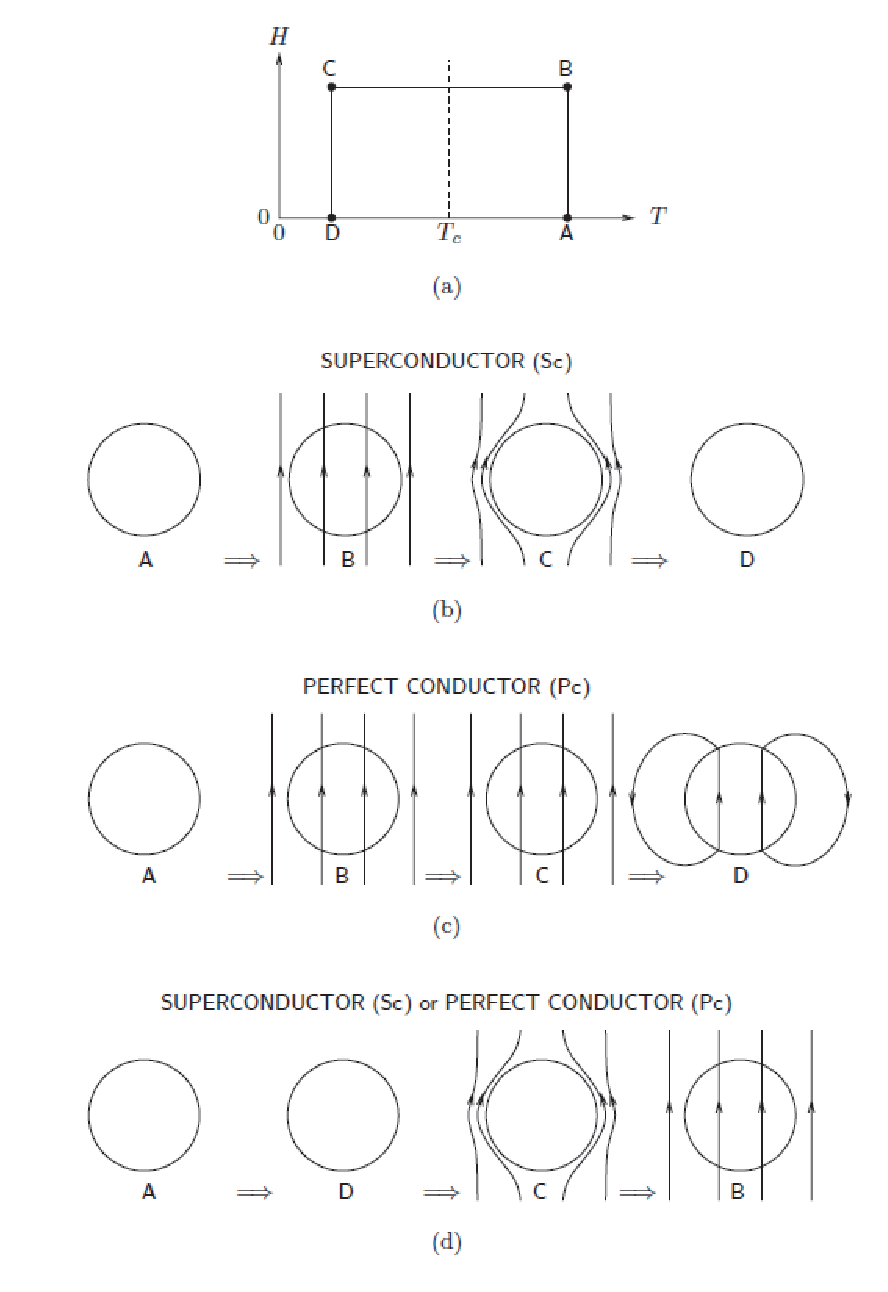
\includegraphics[scale=0.7]{chpt1/figs/fig1.1.eps}
  \caption{
(a): 两个球在$T <T_c$时的H-T相图,其中一个是超导体,另一个是理想导体。
(b): 超导球按$ A\rightarrow B\rightarrow C\rightarrow D$顺序施加H-T环境的磁场情况。
(c): 理想导体按相同的顺序施加H-T环境的磁场情况。
(d): 超导体或理想导体按$A\rightarrow D\rightarrow C\rightarrow B$顺序施加H-T环境的磁场情况。}
\end{figure}

\subsection{超导电性的London理论}
超导电性的唯象理论自1930年代开始发展(微观理论---BCS理论到1957年才完成)。其中,London电磁理论
(1935年)提出``穿透深度"概念来解释Meissner效应。简单的说,穿透深入为$\lambda$的表面超导电流
完全屏蔽了超导体外磁场。根据London理论,$\lambda$由下式给出:
\begin{equation}
\lambda=\sqrt{\frac{m}{\mu_0 e^2 n_{se}}}
\end{equation}
式中,$m$和$e$分别是电子质量($9.11\times 10^{-31}\ \mathrm{kg}$)和电荷量($1.60\times 10^{-19}\ \mathrm{C}$);$\mu_0$是自由空间磁导率($4\pi \times 10^{-7}\ \mathrm{H/m}$)。
这里,超导电子密度$n_{se}$与自由电子$n_{fe}$不同:在$T=0$时,所有电子都是超导电子;在$T=T_c$时,无超导电子。定量地,有:
\begin{equation}
n_{se}\approx n_{fe}=\frac{\rho N_A}{W_A}
\end{equation}
其中,$\rho$是导体的密度($\mathrm{g/cm^3}$),$N_A$是Avogadro常数($6.023\times 10^{23}/\mathrm{mole}$),$W_A$是
原子质量($\mathrm{g/mole}$)。超导电流密度$J_c=e n_{se} v\approx e n_{fe} v$,$v$是超导电子的漂移速度。

\subsection{第I类和第II类超导体}
1911年,Onnes在纯汞中发现了超导电性;随后,铅、锡等其他金属也被发现是超导体。
这些材料,被称为第I类超导体。第I类超导体$H_c$较小(0.1 T),并不适合做超导磁体的材料。
磁体级超导体属第II类,是由Haas和Voogd于1930年首先在铅铋合金中发现。

第II类超导体可以用第I类超导体和正常导体材料的混合态来建模。
1960年代初,有两种混合态物理模型:薄层模型(lamina)和岛模型(island)。
薄层模型是Goodman提出的,他认为第II类超导体的超导态层被正常态层分割开。
岛模型是Abrikosov提出的,不久得到了Essmann和Trauble的实验证实。
该理论认为在超导``海"中存在许多正常态的``岛"。对于第II类超导体,若要在0. 1T以上还能保持超导态,
正常态``岛"的半径必须小于$\lambda$。岛半径是空间参数---相干长度$\xi$,该参数是Pippard在1953年引入的。

$\xi$定义了超导/正常态转变发生的距离。根据用于解释第II类超导体磁场性质的GLAG理论,
如果某超导体的$\xi < \sqrt{2}\lambda$,则属于第II类;$\xi >\sqrt{2}\lambda$,则属于第I类。
合金中由于自由电子的平均自由程缩短,$\xi$减小。
$\xi$反比于材料正常态的电阻率。两种常用的磁体级超导体---$\mathrm{NbTi}$和$\mathrm{Nb_3Sn}$
---的室温正常态电阻率都比铜打出一个数量级。值得注意的是,所有HTS的$\xi$都远小于$\lambda$。

\begin{figure}[htbp]
	\centering
	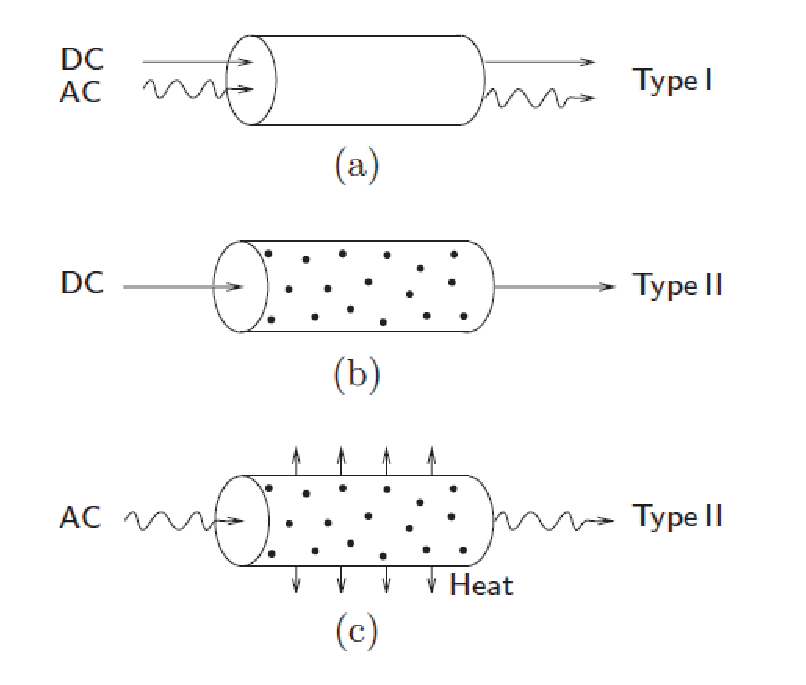
\includegraphics[scale=0.6]{chpt1/figs/fig1.2.eps}
	\caption{
		载流超导棒。 (a) 第I类超导体棒, DC或AC---无焦耳耗散产生;
		(b) 第II类超导体棒,DC无耗散;(c) 第II类超导体棒,AC有焦耳热耗散产生。}\label{acdccurrent}
\end{figure}

\subsubsection{DC和AC响应}
图~\ref{acdccurrent}给出了三根超导棒的示意图。
第I类棒(1.2a)和第II类棒(1.2b,1.2c)中的载流均小于其临界电流。
在第I类超导体中,无论通过AC抑或DC,电流都只在表面(London穿透深度)流过且无能量耗散。
第II类超导体中,DC在整个棒体内流过,尽管存在正常区,但不产生耗散。
我们可以想象为``超导电子"通过材料时``躲"开了正常态区域。
从电路的观点看,可以认为这些有电阻的``岛"被周围的超导``海"短路掉了。
当通以AC时,第II类超导体是有损耗的,即存在电阻---尽管其有效电阻仍然比正常高导电金属小几个数量级。
每一个正常态区域都包含磁通束,称为磁通量子(fluxoid)或旋涡(vortices)。
磁通束在时变磁场和/或电流下``流"动。此种耗散性磁通流动是第II类超导体交流损耗的主要来源。

\subsubsection{磁场性质}
第I类超导体在$H<H_c$下是完全抗磁的;超过$H_c$后就成为常规的无磁材料。
第II类超导体在$H_{c1}$下,磁场性质和第I类一样;在$H_{c1}$和$H_{c2}$之间时,第II类超导体是混合态。
图~\ref{mhcurve}给出了第I类/第II类超导体的磁化强度与磁场强度的关系。
注意,磁体级超导体的磁化曲线都是不可逆的,并非如图中一样。不可逆的结果之一就是存在磁滞。
第II类超导体的磁滞本性是其交流损耗的又一来源。

%%磁化曲线
\begin{figure}[htbp]
  \centering
 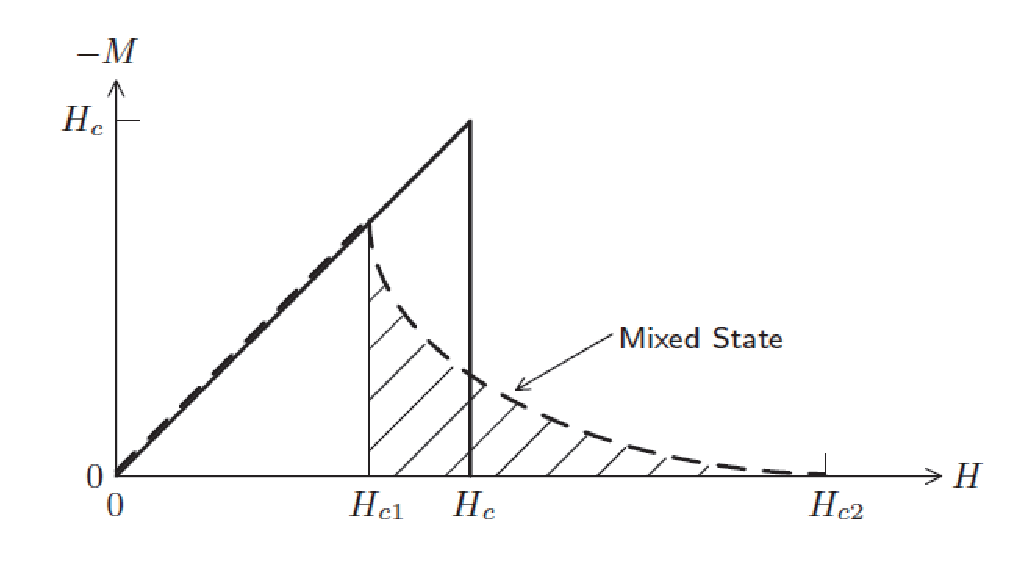
\includegraphics[scale=0.6]{chpt1/figs/fig1.3.eps}
  \caption{
超导体的M-H关系。实线是第I类,虚线是第II类。斜线填充区域表示第II类超导体的混合态。
}\label{mhcurve}
\end{figure}

\subsubsection{超导体举例}
表~\ref{criticalparameters}列出了一些超导体,并给出了其类型、零场临界温度$T_c$、临界磁感应强度
(第I类为$\mu_0H_c$;第II类为$\mu_0H_{c2}$)。所有的金属都是第I类超导体,临界场很小。
这就解释了为什么Onnes在1913年试图用铅线做超导磁体会失败:在很小磁场下,铅就失超了。
即使Onnes时代,磁场也要达到0.3 T才有使用价值。表\ref{criticalparameters}已经很清楚的表明,
超导磁体必须使用第II类超导体。
和第I类超导体不同,第II类超导体存在多种类型:合金、金属混合物甚至氧化物。
所有的高温超导体都是氧化物。$\mathrm{MgB_2}$非金属,也被归为高温超导体。
图~\ref{tcvsyear}给出了几种代表性的HTS或LTS的$T_c$及其发现年份。
图中还标出了重要制冷工质的沸点。
其中,实线把氧化物超导体连缀了起来,虚线把金属超导体连缀了起来。

\begin{table}[htbp]\small%%表1.2
  \centering
  \caption{几种代表性第I类和第II类超导体的临界温度和临界磁场} \label{criticalparameters}
\begin{threeparttable}
  \begin{tabular}{|l|c|c||l|c|c|}
    \hline
    % after \\: \hline or \cline{col1-col2} \cline{col3-col4} ...
    第I类 & $T_c$[K] & $\mu_o H_c$\tnote{*}\ [T] & 第II类 & $T_c$[K] & $\mu_o H_{c2}$\tnote{*}\ [T] \\ \hline 
    Ti & 0.39 & 0.0100 & Nb & 9.5 & 0.2\tnote{*} \\ \hline
    Zr & 0.55 & 0.0047 & NbTi & 9.8 & 10.5\tnote{$\dagger$} \\ \hline
    Zn & 0.85 & 0.0054 &NbN & 16.8 & 15.3\tnote{$\dagger$} \\ \hline
    Al & 1.18 & 0.0105&$\mathrm{MgB_2}$ & 39.0 & 35-60\tnote{$\ddagger$}\\ \hline
    In & 3.41 & 0.0281 & $\mathrm{Nb_3Sn}$ & 18.2 & 24.5\tnote{$\dagger$}  \\ \hline
    Sn & 3.72 & 0.0305  & $\mathrm{Nb_3Al}$ & 18.7 & 31\tnote{$\dagger$}\\ \hline
    Hg & 4.15 & 0.0411  & $\mathrm{Nb_Ge}$ & 23.2 & 35.0\tnote{$\dagger$}\\ \hline
    V & 5.38 & 0.1403& YBCO & 93 & 150\tnote{*}\\ \hline
    Pb & 7.19 & 0.0803 & $\mathrm{Bi_2Sr_2Ca_{n-1}Cu_{n}O_{2n+4}}$\tnote{$\star$} & 85-110 & >100\tnote{*} \\
    \hline
  \end{tabular}
 \begin{tablenotes}
        \footnotesize
        \item[*] 0 K, 估计值。 %此处加入注释*信息
        \item[$\dagger$] 4.2 K, 估计值。%此处加入注释**信息
        \item[$\ddagger$] 4.2 K, 估计值(35 T,平行场,60 T,垂直场)。%此处加入注释**信息
        \item[$\star$] $n=2$, Bi2212; $n=3$, Bi2223。%此处加入注释**信息
      \end{tablenotes}
    \end{threeparttable}
\end{table}


\begin{figure}%%图1.4
  \centering
 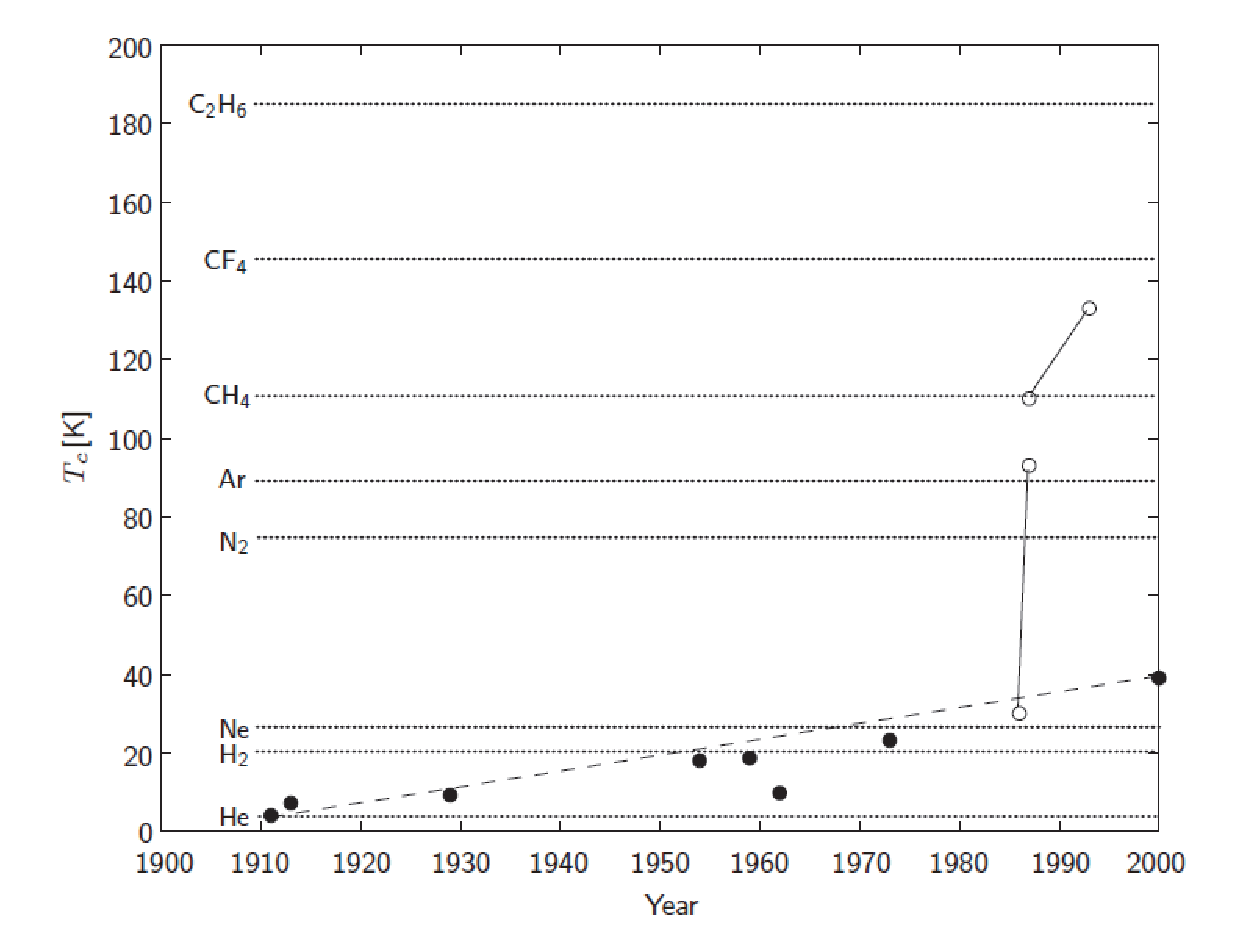
\includegraphics[scale=0.6]{chpt1/figs/fig1.4.eps}
  \caption{
几种代表性超导体$T_c$和发现年份。实线和空心圆圈:高温超导体,HTS;虚线和实心圆圈:低温超导体,LTS(2000年发现的$\mathrm{MgB_2}$除外,其$	T_c=39\ \mathrm{K}$,被认为是HTS)。
水平点线:若干制冷剂的沸点温度,自下而上分别为:$\mathrm{
He(4.22\ K);H_2(20.39\ K);Ne(77.36\ K);N_2(77.36\ K);Ar(87.28\ K);
CH_4(111.6\ K);CF_4(145.4\ K);C_2H_6(184.6\ K)}。$
}
\end{figure}


\subsection{第II类超导体的临界面}
图1.5给出了一种典型的第II类磁体级超导体的临界面。超导电性存在于由边界函数$f_1,f_2,f_3$所确定的临界面之下。对磁体工程师更有用的是通用的$f(H,T,J)$函数。
\begin{figure}
  \centering
 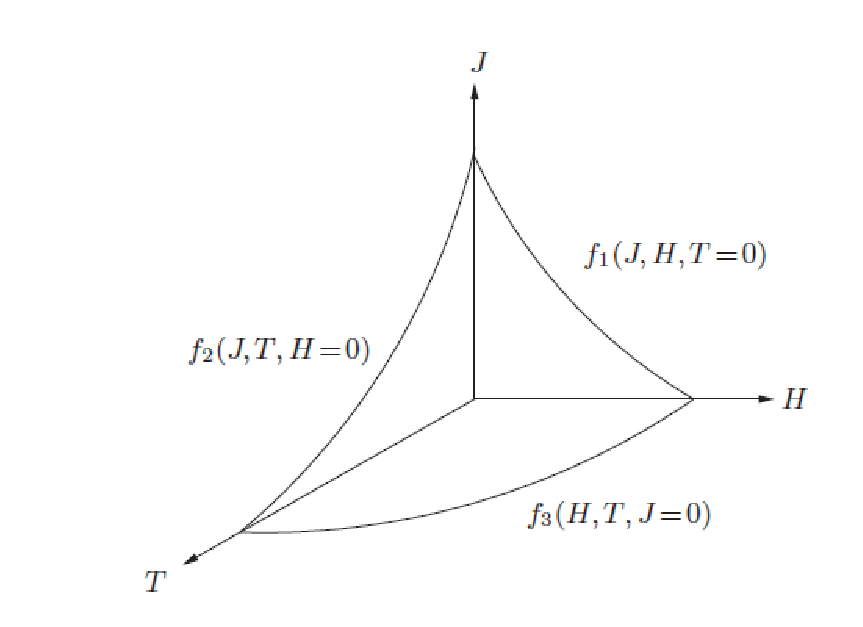
\includegraphics[scale=0.6]{chpt1/figs/fig1.5.eps}
  \caption{
典型第II类超导体的临界面
}\label{ciriticalsurface}
\end{figure}

\subsubsection{临界电流密度,$J_c$}
第II类超导体的$J_c$可以通过金相处理的方式大大提高。这种增强的$J_c$性能通常归因于产生的``钉扎中心"钉住了旋涡,
从而可以抵抗施于其上的Lorentz力($\vec{J}_c\times \vec{B}$)。
钉扎中心可通过材料掺杂、金相处理(如冷处理产生错位,热处理产生前位体和晶界)等手段产生。Kim等给出:
\begin{equation}
  J_c\approx \frac{\alpha_c}{H+H_0}\
\end{equation}
式中,$\alpha_c, H_0$是常数。$\alpha_c$是$H\gg H_0$时与Lorentz力密度平衡的渐近力密度。

\section{磁体级超导体}
磁体级超导体是指那些满足严格的磁体参数要求且可商业化获取的超导体。
以下是对磁体级超导体和超导材料的简明讨论简短评论:现今每一种成功的磁体级超导体,
都经历了长期和复杂的发展过程才从实验室走出。

\begin{table}[htbp]\small
  \centering
  \caption{超导材料 vs. 磁体级超导体} \label{scmaterialvsconductor}
\begin{tabular}{|l|c|l|c|}
  \hline
  标准 & 数量 & 标准 & 数量 \\ \hline
  1. 能超导? & ~10000 & 3. $J_c>1\ \mathrm{GA/m^2}$? & ~10 \\ \hline
  2. $T_c> 4.2\ \mathrm{K}$且$\mu_0 H_{c2}>10\ \mathrm{T}$? &~100 & 磁体级? & <10 \\
  \hline
\end{tabular}
\end{table}

\subsection{超导材料 vs. 磁体级超导体}
表\ref{scmaterialvsconductor}给出了满足特定标准的材料数量。可见,随着标准推向磁体级,数量急剧减少。
实际上,当今发现的10000多种超导体中,仅有几种可用于超导磁体。它们包括低温超导体NbTi、$\mathrm{Nb_3Sn}$;
高温超导体Bi-2212、Bi-2223、YBCO以及$\mathrm{MgB_2}$。

\subsection{实验室级超导体 vs. 磁体级超导体}
超导材料从实验室级到磁体级要经过很长的一段历程。可分为六个阶段:
\begin{enumerate}
  \item 发现;
  \item 提高$J_c$性能
  \item 与基底金属的共处理;
  \item 多丝成形;
  \item $I_c>100\ \mathrm{A}$且长度$>1000\ \mathrm{m}$;
  \item 其他要求,如强度和应力容许值。
\end{enumerate}

表\ref{scstage}给出了$\mathrm{Nb_3Sn}$和Bi-2223的上述六个阶段开始的大致时间。
Bi-2223最开始是与常规金属银共处理的,其阶段2一直持续到今天。
对于涂层YBCO,目前大致处于阶段3晚期,即将进入阶段4。
目前已有使用YBCO制作的运行于77 K的小线圈。
2001年发现的$\mathrm{MgB_2}$已进入阶段5,目前已有``大"$\mathrm{MgB_2}$磁体建成投运。

1961年发现的$\mathrm{Nb_3Sn}$经过十多年紧张的R\&D后,到目前在多数磁体应用时,仍需由用户定制材料性质。
$\mathrm{Nb_3Sn}$的脆性及其承受应力不能超过$~0.3\%$的约束本质上决定了它是不易处理的,
需要十分小心谨慎;BSCCO与此情形很类似。

\begin{table}[htbp]\small
  \centering
  \caption{$\mathrm{Nb_3Sn}$和$\mathrm{Bi-2223}$从材料到导体的发展阶段} \label{scstage}
\begin{tabular}{|c|l|c|c|}
  \hline
  阶段&事件& $\mathrm{Nb_3Sn}$ &Bi-2223 \\ \hline
1 & 发现 & 1950年代早期& 1980年代晚期 \\ \hline
2 & 做成大$J_c$短样 & 1960年代早期 & 1990年代早期\\ \hline
3 &与基底金属共处理&1960年代晚期&1990年代早期\\ \hline
4 &多丝成形&1970年代早期&1990年代中期\\ \hline
5 &$I_c\ge 100\ \mathrm{A}$;长度$\ge 1000\ \mathrm{m}$ &1970年代中期&2000年代早期\\ \hline
6 &其他磁体需求&1970年代晚期&2000年代中期\\
  \hline
\end{tabular}
\end{table}


\section{磁体设计}
\subsection{要求和关键点}
磁体无论直接用于实验还是作为大系统的一个组件,都必须满足磁场的基本要求:规定的空间分布和规定时变特性。
磁场的特性常由以下重要参数给定:1. $H_0$,磁体中心($x=0, y=0, z=0$)场强;
2. $V_0$,规定磁场的空间区域;
3. $H(t)$,磁场的时变特性。其中,特征1和3,在第二章和第三章中有详细讨论。
除了满足以上基本要求,磁体设计还必须满足以下几个关键点:
\begin{description}
  \item[机械完整性] 磁体必须有足够的结构强度,承受正常运行和故障时的巨大磁场应力。
  \item[运行可靠性] 磁体必须能稳定、可靠的达到并持续工作于运行点。
  磁体的这种稳定性,一般简称为磁体稳定性。运行中磁体失去超导电性的过程叫\textbf{``失超"}。
  \item[保护] 一旦发生可能导致磁体变成正常态的事件,必须能保证其不被损坏并且能在事件解除后可再次励磁并
  工作于运行点。
  \item[导体] 对量产的磁体,超导磁体系统的费用很大程度上受超导体费用的影响,即导体费用决定磁体费用。
  本书定量处理少数几个有关多种方案经济性选择的导体费用问题,比如
NbTi@1.8 K,$\mathrm{Nb_3Sn}$@4.2 K,NbTi@4.2 K,$\mathrm{MgB_2}$@15 K。
  \item[制冷] 磁体运行需要能量来创造并维持低温环境,故制冷是超导磁体的一个重要问题。
  人们常过分强调制冷对于整个系统的重要性。故这里必须指出,哪怕在超导磁体是作为关键部件的很多应用中,
  磁体也不过是整个系统的一个组件,而制冷则又是磁体的一个组件。
  制冷系统的功耗通常仅占整个系统的一个很小分数。
\end{description}

磁体的终极发展目标是市场化。若想取得市场成功,还需要考虑两点:1. 价格;2. 易用性。

\subsection{运行温度的影响}
LTS磁体的基本温度通常是4.2 K;仅HTS磁体的运行温度可能高于4.2 K。
运行温度会影响到磁体的五个方面:机械完整性、稳定性、保护、导体和制冷。
图1.6给出了``难度或费用"与运行温度的定性关系。
%图1.6
\begin{figure}
  \centering
 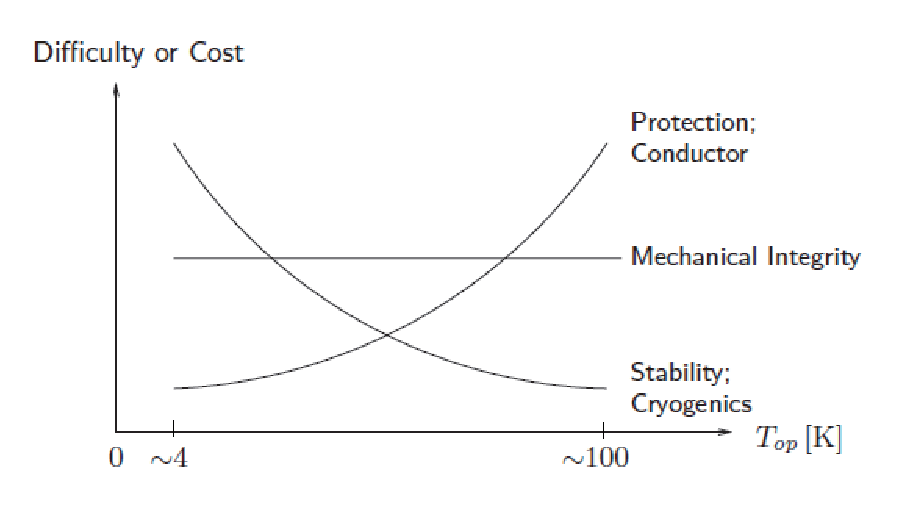
\includegraphics[scale=0.6]{chpt1/figs/fig1.6.eps}
  \caption{
温度对磁体的五个关键点的影响
}
\end{figure}

通常,LTS的运行温区是1.8-10 K,HTS是20-80 K。LTS/HTS混合系统,运行温度由LTS决定,一般<10 K。
图1.6中,保护与导体、稳定性与制冷用同一条曲线,仅表示趋势,并不代表实际上的重合。

图1.6表明,机械完整性的要求基本与运行温度无关。这个结论在运行温度到100 K之间都是适用的。
在这个温区内,磁体的不同材料的热膨胀都可忽略。
对给定磁场要求的磁体,安匝数与运行温度基本无关。因为已知的超导体的临界电流密度都是随温度上升而下降,
而导体费用总是随温度上升而提高:降低制冷费用的期望收益一定要与导体费用的增加值作比较。
运行稳定性和保护受运行温度影响较大。

\section{数值解}
本书开篇已指出,超导磁体技术是一门交叉学科,需要精湛的机械、电气、制冷和材料领域的专业知识。
其实这也意味着一个人是不可能完成满足每一个实际磁体设计和运行参数需求的可靠的数值解的。
通常,需要一个专业的团队来做成此事。
\subsection{粗算解}
制冷工程师或其他成员没必要对磁场专家的所有计算深信不疑,制冷专家也应当能够计算比较复杂条件下的大致磁场。
本书的一个目标就是让设计团队的每一个成员都具备在自己领域以及其他领域进行估算的能力。
实际上,每一个新磁体系统的研发都应以此开始:每一个成员都来对每一个重要的设计和运行参数粗算一遍;
而后,由组内领域专家完成磁体制造和运行的更精确的数值计算。

\subsection{程序解}
磁体系统的实际制造和运行的每一个设计和运行参数一般都必须采用程序辅助计算。
多数设计团队使用ANSYS、VectorFields、COMSOL,这几种软件都可用于磁场、应力应变以及热的分析。
GANDALF、THEA等专用程序专门用于处理CICC导体绕制的大型磁体(特别是聚变磁体)的失超产生和传播现象。
失超现象包含的热、流体、电暂态、电缆和工质等的变化很大,热、电物性的变动幅度常跨越1-2个数量级。
正是这个原因,失超暂态多(有时完全是)依赖于数值仿真。数值仿真能处理非线性的热能产生和传导以及工质因受热引起的可压缩黏性流动。
上述每一套程序都凝结了大量专家超过25年的大量工作。

GANDALF和THEA都是商业软件。GANDALF最初是用来分析ITER导体的热-流体暂态的。THEA的主要特征是将热、流体模型扩展到多平行通道。
%【此句不通】如多丝具有不同温度,平行流通道,包括非均一电流分布和暂态重分配。

\section{专题}
\subsection{问题1.1:第I类超导体的热力学性质}
第I类超导体的单位体积比热($\mathrm{J/m^2K}$)由下式给出:
\begin{subequations}\label{eqn:1.4ab}
	\begin{align}
\mbox{超导态:} C_s(T) &= aT^3 \\
\mbox{正常态:} C_n(T)&= bT^3+\gamma T	
	\end{align}
\end{subequations}
式中,$a,b,\gamma$都是常数。

a) 证明零场时的临界温度为:
\begin{equation}\label{eqn:1.5}
  T_c=\sqrt{\frac{3\gamma}{a-b}}
\end{equation}
提示:1) 熵的表达式$C(T)=T\frac{\partial S(T)}{\partial T}$;2) $H=0$时,有$S_n(T_c)-S_s(T_c)=0$。

b) 证明$H_{c0}$在$T$=0 K,$H_{c0}\equiv H_c(0)$时,可由下式给出:
\begin{equation}\label{eqn:1.6}
  H_{c0}=T_c \sqrt{\frac{\gamma}{2\mu_0}}
\end{equation}

证明临界磁场$H_c(T)$是$T$的二次函数:
\begin{equation}\label{eqn:1.7}
  H_c(T)=H_{c0}\left[1-\left(\frac{T}{T_c}\right)^2\right]
\end{equation}
提示:零场时单位体积的吉布斯自由能关系为:
\begin{equation}\label{eqn:1.8}
  G_n(T)-G_s(T)=\frac{1}{2}\mu_0 H_c^2(T)
\end{equation}
根据1.8式以及$S(T)=-\partial G(T)/\partial T$,可以推导出1.6式。

c) 证明内能密度差$U_n-U_s$在自场下于$T_{ux}$时取最大:
\begin{equation}
  T_{ux}=\frac{T_c}{\sqrt{3}}
\end{equation}
提示:在零场时有$U(T)=\int C(T)dT$。

d) 缓慢绝热地向超导磁体施加磁场(初始温度为$T_i$,$0<T_i<T_c$)至略大于其临界值,
此时超导体相变为正常态。降低导体温度到$T_j (<T_i)$,给出$T_i$和$T_j$的关系,并
画出本过程的热力学相图。

e) 同样对d)中的超导体,初始温度为$T_i$($0<T_i<T_c$),置于零场中,突然施加$H_e$。
如果$H_e$超过临界值$H_{ec}$,材料将被加热。证明
\begin{equation}
  H_{ec}(T_i)=H_c(T _i)\sqrt{\frac{1+3(T_i/T_c)^2}{1-(T_i/T_c)^2}}
\end{equation}

\subsubsection{问题1.1之解答}
a) 由于$C(T)=T\frac{\partial S(T)}{\partial T}$以及$S(T=0)=0$,我们有
\begin{align*}
S(T) =\int_{0}^{T}C(T)dT \tag{S1.1} 
\end{align*} 

将1.4式代入,有:
\begin{align*}
S_s(T) =\int_{0}^{T}\frac{C_s(T)}{T}dT=\frac{1}{3}aT^3 \tag{S1.2a}
\end{align*} 
\begin{align*}
S_n(T) =\int_{0}^{T}\frac{C_n(T)}{T}dT = \frac{1}{3}bT^3 + \gamma T \tag{S1.2b}
\end{align*} 

于是,
\begin{align*}
S_n(T) − S_s(T) =\gamma T − \frac{1}{3} (a − b)T^3\tag{S1.3}
\end{align*} 

上文已指出,在$H=0$时,有$S_n(T_c)−S_s(T_c)=0$,所以
\begin{align*}
\gamma= \frac{1}{3} (a − b)T^2 \tag{S1.4}
\end{align*}

解出$T_c$,有
\begin{align*}
T_c=\sqrt{\frac{3\gamma}{a-b}} \tag{1.5}
\end{align*}

b) 从式1.8以及$S(T)=−\partial G(T)/\partial T$,有
\begin{align*}
S_n(T) − S_s(T) = −\mu_0 H_c(T)\frac{\partial H_c(T)}{\partial T}\tag{S1.5}
\end{align*}

联立S1.3和S1.4,并利用$(a-b)/3=\gamma/T_c^2$,有
\begin{align*}
S_n(T) − S_s(T)=\gamma T\left[1-\left(\frac{T}{T_c}\right)^2\right]  \tag{S1.6}
\end{align*}

联立上面两式,对$T$积分,有
\begin{align*}
−\frac{1}{2}\mu_0 H_c^2(T) =\frac{1}{2}\gamma T_c^2-
\frac{1}{4}\gamma T_c^2 \left(\frac{T}{T_c}\right)^4+A \tag{S1.7}
\end{align*}
式中,$A$是常数。由于$H_c(T =0)\equiv H_{c_0}$,我们有$A=−\mu_0 H_{c_0}^2 / 2$。在
$T=T_c$时,由于$H_c(T_c)=0$,上式成为
\begin{align*}
0=\frac{1}{2}\gamma T_c^2-\frac{1}{4}\gamma T_c^2-\frac{1}{2}\mu_0 H_{c_0}^2\tag{S1.8}
\end{align*}

解出$H_{c_0}$,有
\begin{align*}
H_{c_0}=T_c\sqrt{\frac{\gamma}{2\mu_0}}\tag{1.6}
\end{align*}

从上式,可以得到
\begin{align*}
\gamma=\frac{2\mu_0 H_{c_0}^2}{T_c^2}\tag{S1.9}
\end{align*}

联立S1.7和上式,得到
\begin{align*}
-\frac{1}{2}\mu_0 H_c^2(T)=\mu_0 H_{c_0}^2 \left(\frac{T}{T_c}\right)^2-\frac{1}{2}\mu_0 H_{c_0}^2 \left(\frac{T}{T_c}\right)^4-\frac{1}{2}\mu_0 H_{c_0}^2\tag{S1.10}
\end{align*}

上式可以重写为:
\begin{align*}
H_c^2(T)=H_{c_0}^2\left[1-2\left(\frac{T}{T_c}\right)^2+\left(\frac{T}{T_c}\right)^4\right]=H_{c_0}^2\left[1-\left(\frac{T}{T_c}\right)^2\right]^2\tag{S1.11}
\end{align*}

从上式,可以得到:
\begin{align*}
H_c(T)=H_{c_0}\left[1-\left(\frac{T}{T_c}\right)^2 \right]\tag{1.7}
\end{align*}

我们可以根据第I类超导体实验测得的$\gamma$和$T_c$通过1.6式预测$H_{c_0}$。
表1.5给出了由公式计算的和实测的$\mu_0 H_{c_0}$数据;同时还给出了一些其他实测数据。
%表1.5
\begin{table}[htbp]\small
  \centering
  \caption{$H_{c_0}$:公式\ref{eqn:1.6}计算值和实测值} \label{tb:eqn1.6andexp}
\begin{tabular}{|c||c|c|c|c|c|c|}
  \hline
第I类超导体&$\rho [\mathrm{g/cm^3}]$&$M [\mathrm{g/mole}]$&$\gamma [\mathrm{J/m^3K^2}]$&$T_c [\mathrm{K}]$&$\mu_0 H_{c_0}$计算&$\mu_0 H_{c_0}$实测 \\ \hline \hline
Ti&4.53&47.88&316.8&0.39&5.6&10.0 \\ \hline
Zr&6.49&91.22&199.2&0.55&6.1&4.7\\ \hline
Zn&7.14&65.38&69.8&0.85&5.6&5.4\\ \hline
Al&2.70&26.98&135.1&1.18&10.9&10.5\\ \hline
In&7.31&114.8&107.6&3.41&28.0&28.1\\  \hline
Sn&7.31&118.7&109.6&3.72&30.9&30.5\\  \hline
Hg&13.55&200.6&120.9&4.15&36.2&41.1\\  \hline
V&6.11&50.94&1111&5.38&142.7&140.3\\  \hline
Pb&11.35&207.2&163.2&7.19&72.8&80.3 \\  \hline
\end{tabular}
\end{table}

c) 由零场时的$dU(T)=C(T)dT$,我们可以得到
\begin{equation*}
U(T) =\int_{0}^{T}C(T) dT  \tag{S1.12}
\end{equation*}

代入1.4式,得
\begin{equation*}
U_n(T) =\int_{0}^{T}(bT^3 +\gamma T)dT = \frac{1}{4}bT^4 +\frac{1}{2}\gamma T^2 \tag{S1.13a}
\end{equation*}
\begin{equation*}
U_s(T)=\frac{1}{4}aT^4 \tag{S1.13b}
\end{equation*}

两个自由能的差表示为:
\begin{equation*}
\begin{split}
U_n(T) − U_s(T) =&\frac{1}{4} (b − a)T^4 + \frac{1}{2}\gamma T^2\\
=&\left(\frac{a-b}{4}\right)\left[\frac{2\gamma}{a-b}T^2-T^4\right]
\end{split} \tag{S1.14}
\end{equation*}

对上式微分,并在$T=T_{ux}$处令其为零,有:
\begin{equation*}
\frac{d(U_n-U_s)}{dT}|_{T_{ux}}=\frac{a-b}{4} \left[\frac{4\gamma}{a-b}T_{ux}-4T_{ux}^3\right]=0 \tag{S1.15}
\end{equation*}

于是
\begin{equation*}
\frac{4\gamma}{a-b}T_{ux}-4T_{ux}^3=0 \tag{S1.16}
\end{equation*}

结合1.5式,解出$T_{ux}$,得
\begin{equation*}
T_{ux}=\sqrt{\frac{\gamma}{a-b}}=\frac{T_c}{\sqrt{3}} \tag{1.9}
\end{equation*}

d) 由于这个过程是绝热和可逆的,那么如果磁场是缓慢施加的,有$S_n(T)=S_s(T)$。从S1.2可以得到
\begin{equation*}
S_n(T_f ) − S_s(T_i) =\frac{1}{3}bT_f^3 +\gamma T_f −\frac{1}{3}aT_i^3 \tag{S1.17}
\end{equation*}

由$S_n(T_f )−S_s(T_i)=0$,我们得到关于$T_f$和$T_i$的表达式
\begin{equation*}
\frac{1}{3}bT_f^3 +\gamma T_f =\frac{1}{3}aT_i^3 \tag{S1.18}
\end{equation*}

由方程1.5,我们有:
\begin{equation*}
b = a − \frac{3\gamma}{T_c^2} \tag{S1.19}
\end{equation*}

联立上面两式,有
\begin{align*}
\frac{1}{3}a(T_f^3-T_i^3)=-\gamma T_f\left[ 1-\left(\frac{T_f}{T_c}\right)^2\right]\tag{S1.20}
\end{align*}

由于$T_f<T_c$,上式的右侧是负值,于是可知$T_f<T_i$。图1.7给出了超导态(实线)和正常态(虚线)
的T-S图。$T_i\rightarrow T_f$转变在图中用竖实线表示。

\begin{figure}
  \centering
 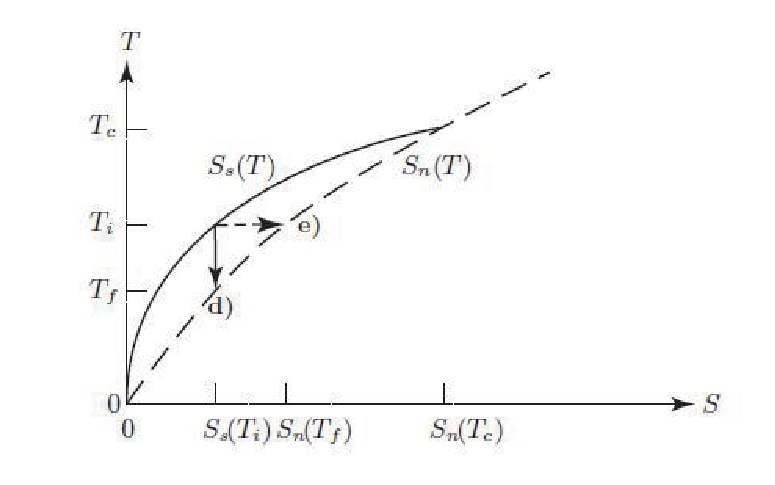
\includegraphics[scale=0.7]{chpt1/figs/fig1.7.eps}
  \caption{超导态(实线)和正常态(虚线)的T-S图}\label{fig:tsplot}
\end{figure}

e) 超导体被加热,首先必须先进入正常态。外场提供磁能$\mu_0 H_c^2(T_i)/2$;由于转变过程要吸热
$T_i[S_n(T_i)-S_s(T_i)]$,故还必须提供吸收能$H_{ec}$。图1.7中的横虚线就是转变过程。于是,
\begin{align*}
\frac{1}{2}\mu_0 H_{ec}^2(T_i)=\frac{1}{2}\mu_0 H_c^2(T_i)+T_i[S_n(T_i)-S_s(T_i)]\tag{S1.21}
\end{align*}

上式和S1.1联立,得到
\begin{align*}
\frac{1}{2}\mu_0 H_{ec}^2(T_i)=\frac{1}{2}\mu_0 H_c^2(T_i)+T_i\left[\frac{1}{3}(b-a)T_i^3+\gamma T_i\right] \tag{S1.22}
\end{align*}

把S1.9代入上式,并应用S1.19,得到
\begin{align*}
\frac{1}{2}\mu_0 H_{ec}^2(T_i)=\frac{1}{2}\mu_0 H_c^2(T_i)+2\mu_0 H_{c_0}^2\left(\frac{T_i}{T_c}\right)^2 \left[1-\left(\frac{T_i}{T_c}\right)^2 \right] \tag{S1.23}
\end{align*}

联立式1.7,得到
\begin{align*}
H_{ec}^2(T_i)=H_c^2(T_i)+4H_c^2(T_i)\frac{(T_i/T_c)^2}{1-(T_i/T_c)^2} \tag{S1.24}
\end{align*}

于是
\begin{align*}
H_{ec}(T_i)=H_c(T_i)\sqrt{\frac{1+3(T_i/T_c)^2}{1-(T_i/T_c)^2}}
\end{align*}

由于$H_c(T_c)=0$,可知$H_{ec}(T_c)=0$;另有$H_{ec}(T_i)\ge H_c(T_i)$。


\subsection{问题1.2:超导回路}
本问题表明,仅通过外接电源才能在闭合超导回路、线圈或盘中产生持续电流。
此处用电路模型证明,参数如图\ref{scloop}。
 
a) 写出两个回路的电路方程。

b) 解出$I_s(t)$,证明以一个初始态和末态都是0的$I(t)$($I(t=0)=I(t=\infty)=0$)不能建立起闭合回路的电流。
闭合超导回路可以是一个采用超导中间接头连接引线的超导磁体、超导盘片、超导盘片堆叠体、圆心有空的超导盘片或
圆心有孔的超导盘片堆叠体。

%图
\begin{figure}[htbp]
  \centering
 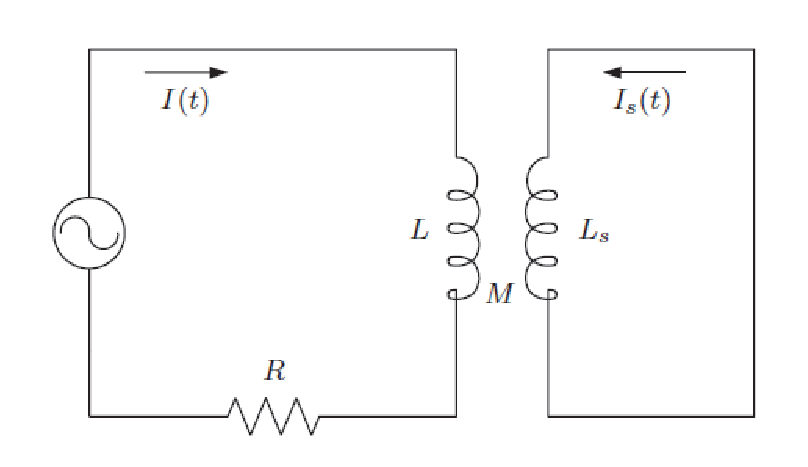
\includegraphics[scale=0.6]{chpt1/figs/fig1.8.eps}
  \caption{
超导线圈回路与一个带有电流源的回路通过电感耦合
}\label{scloop}
\end{figure}

\subsubsection{问题1.2之解答}
a) 两个电压方程为
\begin{align*}
L\frac{dI(t)}{dt}+M\frac{dI_s(t)}{dt}+ RI(t) = 0 \tag{S2.1a}
\end{align*}
\begin{align*}
M\frac{dI(t)}{dt}+ L_s\frac{dI_s(t)}{dt}= 0 \tag{S2.1b}
\end{align*}

b) 从S2.1b中可以解得
\begin{align*}
I_s(t) = −\frac{M}{L_s}I(t) + C\tag{S2.2}
\end{align*}

因为$I_s(t=0)=0$,所以,$C=0$。由于$I(t=0)=I(t=\infty)=0$,所以仅在$I(t)\neq 0$时有$I_s(t)\neq 0$。
也即,无外流源也无初始值的超导回路不能孤立的维持能量。

在一个超导回路中不能产生感应电流在某些应用中是有实际意义的。持续运行模式的磁体必须通过引线通入电流
充电(处于励磁模式)。此后,通过所谓的``超导开关"(persistent current switch,PCS)将引线短路后电源可以退出。


\subsection{问题1.3:磁共振成像(MRI)}
超导磁体最成功的商业应用之一便是医疗诊断装置,特别是MRI。以下是磁体工程师需要了解的一些基本问题:

a) MRI中,为什么$H^1$、$N^{14}$核可以被探测到,而$C^{12}$、$O^{16}$核探测不到?

b) 如果频率分辨率10 Hz,对于1 T全身MRI磁体的中心磁场均匀性最小要求多少?对室温孔直径80 cm的全身MRI磁体,
上述均匀场区域通常在25 cm DSU(直径半球体积)。

c) MRI单元中,脉冲梯度磁体的作用?

d) 对1 T磁体单元,脉冲磁体产生的典型$\frac{d\vec{B}}{dz}$是多少?

\subsubsection{问题1.3之解答}
a) 有奇数核子的原子核存在净角动量。处于磁场中,原子核按某种正比于磁场强度的特定频率(Larmor)进动。
比如氢的Larmor频率在1 T时是42.576 MHz。表1.6\footnote{加粗的数字表示可探测}给出了几种物质原子的数据。
%表1.6
\begin{table}[htbp]\small
  \centering
  \caption{几种元素的原子核数据} \label{tb:atomic}
\begin{tabular}{|c|c|c|c|c|c|}
  \hline
原子序数&元素&原子质量&质子数&中子数&可探测? \\ \hline \hline
1&氢&1&\textbf{1}&0&是 \\ \hline
6&碳&12&6&6&否 \\ \hline
6&碳&13&6&\textbf{7}&是 \\ \hline
7&氮&14&\textbf{7}&\textbf{7}&是 \\ \hline
8&氧&16&8&8&否 \\ \hline
11&钠&23&\textbf{11}&12&是 \\ \hline
15&磷&31&\textbf{15}&16&是 \\ \hline
\end{tabular}
\end{table}

b) 10 Hz相当于 $42.576×10^6$ Hz的$0.23×10^{−6}$,所以磁场必须是1 T的$0.23×10^{−6}$ ,
大约是 $0.002\ \mathrm{gauss}$。作为对比,地磁场约为$0.7 \ \mathrm{gauss}$。

c) 通过引入特定的空间磁场分布,我们可以限制在某个指定区域产生共振。
这让我们可以对某一个特定核素进行成像。

d) 梯度幅值直接和成像的空间解析度相关。更高的梯度相应产生更好的解析度。但存在一个磁体
和患者可以忍受的极限问题。医用MRI必须限制梯度强度---至少应限制梯度偏斜率---以避免产生对神经
和肌肉的刺激。医用MRI的最大梯度约为$3-4 \ \mathrm{gauss/cm}$,最大场偏斜率约为$12\ \mathrm{(gauss/cm)/ms}$或者
$120\ \mathrm{(T/m)/s}$。

\section*{参考文献}
[1.1] J.K. Hulm and B.T. Matthias, ``Overview of superconducting materials development,”
in Superconductor Materials Science—Metallurgy, Fabrication, and Applications,
Eds., S. Foner and B.B. Schwartz (Plenum Press, NewYork, 1981).

[1.2] A.A. Abrikosov, ``On the magnetic properties of superconductors of the second
type (English translation),” Zh. Eksp. Teor. Fiz. (Soviet Union) 5, 1174 (1957).

[1.3] U. Essmann and H. Tr¨auble, ``The direct observation of individual flux lines in
Type II superconductors,” Phys. Lett. 24A, 526 (1967).

[1.4] Y.B. Kim, C.F. Hempstead, and A.R. Strnad, ``Magnetization and critical supercurrents,” Phys. Rev. 129, 528 (1963).

[1.5] J.K. Hoffer, ``The Initiation and propagation of normal zones in a force-cooled
tubular superconductor,” IEEE Trans. Mag. 15, 331 (1979).

[1.6] C. Marinucci, M.A. Hilal, J. Zellweger, and G. Vecsey, ``Quench studies of the
Swiss LCT conductor,” Proc. 8th Symp. on Eng. Prob. Fus. Res., 1424 (1979).

[1.7] V.D. Arp, ``Stability and thermal quenches in force-cooled superconducting cables,”
Proc. of 1980 Superconducting MHD Magnet Design Conference, MIT, 142(1980).

[1.8] J. Benkowitsch and G. Kraft, ``Numerical analysis of heat-induced transients in
forced flow helium cooling systems,” Cryogenics 20, 209 (1980).

[1.9] E.A. Ibrahim, ``Thermohydraulic Analysis of Internally Cooled Superconductors,”
Adv. Cryo. Eng. 27, 235 (1982).

[1.10] C. Marinucci, ``A numerical model for the analysis of stability and quench characteristics of forced-flow cooled superconductors,” Cryogenics 23, 579 (1983).

[1.11] M.C.M. Cornellissen and C.J. Hoogendoorn, ``Propagation velocity for a force
cooled superconductor,” Cryogenics 25, 185 (1985).

[1.12] A.F. Volkov, L.B. Dinaburg, and V.V. Kalinin, ``Simulation of helium pressure
rise in hollow conductor in case of superconductivity loss,” Proc. 12th Int. Cryo.
Eng. Conf. (Southampton, UK), 922 (1988).

[1.13] R.L. Wong, ``Program CICC flow and heat transfer in cable-in-conduit conductors,”
Proc. 13th Symp. Fus. Tech. (Knoxville, TN), 1134 (1989).

[1.14] L. Bottura and O.C. Zienkiewicz, ``Quench analysis of large superconducting magnets. Part I: model description,” Cryogenics 32, 659 (1992).

[1.15] C.A. Luongo, C.-L. Chang, and K.D. Partain, ``A computational model applicable
to the SMES/CICC,” IEEE Trans. Mag. 30, 2569 (1994).

[1.16] A. Shajii and J.P. Freidberg, ``Quench in superconducting magnets. I. Model and
implementation,” J. Appl. Phys. 76, 3149 (1994); ``Quench in superconducting
magnets. II. Analytic Solution,” J. Appl. Phys. 76, 3159 (1994).

[1.17] R. Zanino, S. De Palo, and L. Bottura, ``A two-fluid code for the thermohydraulic
transient analysis of CICC superconducting magnets,” J. Fus. Energy 14,
25 (1995).

[1.18] L. Bottura, ``A numerical model for the simulation of quench in the ITER magnets,”
J. Comp. Phys. 125, 26 (1996).

[1.19] L Bottura, C. Rosso, and M. Breschi, ``A general model for thermal, hydraulic,
and electric analysis of superconducting cables,” Cryogenics 40, 617 (2000).

[1.20] Q. Wang, P. Weng, and M. Hec, ``Simulation of quench for the cable-in-conduitconductor in HT-7U superconducting Tokamak magnets using porous medium
model,” Cryogenics 44, 81 (2004).

[1.21] T. Inaguchi, M. Hasegawa, N. Koizumi, T. Isono, K. Hamada, M. Sugimoto, and
Y. Takahashi, ``Quench analysis of an ITER 13T-40kA Nb3Sn coil (CS insert),”
Cryogenics 44, 121 (2004).

[1.22] L. Bottura, ``Numerical aspects in the simulation of thermohydraulic transients
in CICC’s,” J. Fus. Energy 14, 13 (1995).

[1.23] L. Bottura and A. Shajii, ``Numerical quenchback in thermofluid simulations of
superconducting magnets,” Int. J. Num. Methods Eng. 43, 1275 (1998).

[1.24] L. Bottura, ``Modelling stability in superconducting cables,” Physica C 316 (1998).

[1.25] A.B. Pippard, The Elements of Classical Thermodynamics (Cambridge University
Press, Cambridge, 1966).

[1.26] C. Kittel, Introduction to Solid State Physics 3rd Ed. (John Wiley \& Sons, 1966).

\newpage
\chapter{电磁场}
\section{引言}
本章我们通过Maxwell方程组来回顾电磁理论。这个回顾是为了“唤起”读者对电磁理论的理解,以便本书的主题——超导磁体——可以
用量化的方式展开。之后,给出了几个在的大多数磁体应用中用得到,并可以用解析方法进行分析的特例,作为专题研究材料。
\section{Maxwell方程}
Maxwell方程组包括四个基本方程:1)Gauss定律;2)Ampere定律;3)Faraday定律;4)磁通连续定律。此外,我们还会常用到电荷守恒方程
和其他本构关系。以下简要的逐一讨论。

本书中如非指明,电磁量都采用SI单位(表\ref{emquantity})。磁体界常常将磁场强度$\vec{H}$和磁通密度(或磁感应强度)$\vec{B}$混用,尽管这个做法
无伤大雅,也基本不会导致混淆,但我们应该提起注意,比如从$\vec{M} vs. \vec{H}$图计算能量的时候。

自由空间的磁导率$\mu_0=4\pi \times 10^{-7} H/m$;自由空间磁导率$\epsilon_0=\frac{1}{\mu_0c^2}$,近似值为$8.85\times 10^{-12} F/m$。
附录IA给出了其他物理常数及部分常用非SI单位到SI单位的转换因子。

电流密度是超导磁体磁场$\vec{H}$的主要源。故相对较小的时变$\vec{D}$场对$\vec{H}$的贡献在本章的Maxwell方程中并未包括进来。

\begin{table}[htbp]\small
  \centering
  \caption{电磁量} \label{emquantity}
\begin{tabular}{|c||l|l|}
  \hline
  % after \\: \hline or \cline{col1-col2} \cline{col3-col4} ...
  符号 & 名称 & SI单位 \\ \hline \hline
  $E$&电场&[V/m] \\ \hline
  $H$&磁场&[A/m] \\ \hline
  $B$&磁感应强度&[T]\\ \hline
  $J$&电流密度&[$A/m^2$] \\ \hline
  $K$&面电流密度&[A/m]\\ \hline
  $\rho_c$&电荷密度&[$C/m^3$]\\ \hline
  $\sigma_c$&面电荷密度&[$C/m^2]$\\ \hline
  $\rho_e$&电阻&[$\Omega m$]\\
  \hline
\end{tabular}
\end{table}

\subsection{电场Gauss定律}
积分形式的自由空间的电场Gauss定律为:
\begin{equation}\label{eqn:gausslaw}
\oint_S \epsilon_o\vec{E}\cdot d\vec{A}=\int_V\rho_c dV
\end{equation}

$\epsilon_0\vec{E}$场的面积分等于表面S围成的体积V内的净电荷量。式\ref{eqn:gausslaw}中,$d\vec{A} =\vec{n}dS$,其中$\vec{n}$是表面元上指向外向
的单位法矢量。从\ref{eqn:gausslaw}得微分形式:
\begin{equation}\label{eqn:gausslaw diff}
  \epsilon_0 \nabla \cdot \vec{E}=\rho_c
\end{equation}

\textbf{边界条件}:在电荷密度为$\sigma_c[C/m^2]$的面上,从区域1到区域2的电场法向分量不连续:
\begin{equation}\label{eqn:gauss bc}
  \vec{n}_{12}\cdot (\vec{E}_2-\vec{E}_1)=\sigma_c/\epsilon_0
\end{equation}

式中,单位矢量$\vec{n_{12}}$从区域1指向区域2。

\subsection{Ampere定律}
积分形式的Ampere定律为:
\begin{equation}\label{eqn:amperelaw}
\oint_C \vec{H}\cdot d\vec{S}=\int_S \vec{J}_f d\vec{A}
\end{equation}

方程表明,$\vec{H}$场的线积分等于C围成的面S内的总的“自由”电流,即不含有磁化电流。微分形式:
\begin{equation}\label{eqn:amperelaw diff}
   \nabla \times \vec{H}=\vec{J}_f
\end{equation}

上述两个方程都没有计入$\vec{H}$的另一个可忽略的源:$\frac{\partial{\vec{E}}}{\partial{t}}$
\textbf{边界条件}:如果存在“自由”面电流密度$\vec{K}_f[A/m]$,则通过区域1到区域2的磁场在切向不连续,满足:
\begin{equation}\label{eqn:ampere bc}
  \vec{n}_{12}\times (\vec{H}_2-\vec{H}_1)=\vec{K}_f
\end{equation}

\subsection{Faraday定律}
积分形式的Faraday定律为:
\begin{equation}\label{eqn:faradaylaw}
\oint_C \vec{E}\cdot d\vec{S}=-\frac{d}{dt}\int_S \vec{B}\cdot d\vec{A}
\end{equation}

方程表明,$\vec{E}$场的线积分等于由C围成的面S内的总磁通对时间变化的负值。微分形式:
\begin{equation}\label{eqn:faradaylaw diff}
   \nabla \times \vec{E}=-\frac{\partial{\vec{B}}}{\partial{t}}
\end{equation}

\textbf{边界条件}:通过区域1到区域2的$\vec{E}$场的切向分量总是连续的:
\begin{equation}\label{eqn:faraday bc}
  \vec{n}_{12}\times (\vec{E}_2-\vec{E}_1)=0
\end{equation}

\subsection{磁通连续性}
积分形式磁通连续性方程为:
\begin{equation}\label{eqn:bcontinuelaw}
\oint_S \vec{B}\cdot d\vec{A}=0
\end{equation}

方程表明,$\vec{B}$场在表面S上的面积分为0,即$\vec{B}$场无点源。微分形式:
\begin{equation}\label{eqn:bcontinuelaw diff}
  \nabla \cdot \vec{B}=0
\end{equation}

\textbf{边界条件}:通过区域1到区域2的$\vec{B}$场的法向分量是连续的,即:
\begin{equation}\label{eqn:bcontinuelaw bc}
  \vec{n}_{12}\cdot (\vec{B}_2-\vec{B}_1)=0
\end{equation}

下文会谈到,在磁介质中,$\vec{B}$是磁场强度$\vec{H}$和磁化强度$\vec{M}$之叠加。这意味着不论两种介质的磁化是多么不同,
$\vec{B}$场在两种介质中的法向分量连续性都可以保持。

\subsection{电荷守恒}
“自由”电流密度$\vec{J}_f$与“自由”电荷密度$\rho_{cf}$的时变率有关。积分形式为:
\begin{equation}\label{eqn:chargelaw}
\oint_S \vec{J}_f\cdot d\vec{A}=-\frac{d}{dt}\int_V \rho_{cf}d\vec{V}
\end{equation}

微分形式为:
\begin{equation}\label{eqn:chargelaw diff}
   \nabla \cdot \vec{J}_f=-\frac{\partial{\rho_{cf}}}{\partial{t}}
\end{equation}

\subsection{本构关系}
磁感应强度$\vec{B}$,磁场强度$\vec{H}$和磁化强度$\vec{M}$的关系为:
\begin{equation}\label{eqn:bhm}
\vec{B}=\mu_0(\vec{H}+\vec{M})
\end{equation}

在同质、各向同性、线性介质(本书通常以此设定为前提)中,$\vec{B}=\mu \vec{H}=\mu_0(1+\chi)\vec{H}$。式中的磁导率$\mu$和磁化系数$\chi$
我们一般假定其与磁场无关。铁磁材料如“高$\mu$”屏蔽材料的$\chi$可高达$10^6$。典型的顺磁材料,例如氧,$\chi=10^{-6}$;抗磁材料如单原子气体、多数液体的
磁化系数是负值。第I类超导体具有完全抗磁性,有$\chi=-1, \mu=0$。

导体材料如金属中,电场$\vec{E}$会激发出电流密度$\vec{J}$,其关系为
\begin{equation}\label{eqn:ohmlaw}
  \vec{J}=\frac{\vec{E}}{\rho_e}
\end{equation}

式中,$\rho_e$是金属的电阻率$[\Omega m]$。

\section{准静态}
电场$\vec{E}$和磁场$\vec{B}$通过法拉第定律耦合在一起。自由空间里,必须解如下的完整方程组:
\begin{eqnarray}\label{eqn:maxwelleqns}
\nabla \cdot \epsilon_0\vec{E} &=&\rho_c \nonumber \\
\nabla \times \vec{E} &=&-\frac{\partial{B}}{\partial{t}} \nonumber \\
\nabla \times \vec{H} &=&\vec{J}_f+\epsilon_0 \frac{\partial{E}}{\partial{t}} \nonumber \\
\nabla \cdot \vec{B} &=&0 \nonumber \\
\nabla \cdot \vec{J}_f &=&-\frac{\partial{\rho_{cf}}}{\partial{t}}
\end{eqnarray}

如果电场$\vec{E}$和磁场$\vec{B}$能够解耦,将大大简化解方程组\ref{eqn:maxwelleqns}的难度。“准静态”分析可以满足很多重要的实际应用。
最简单的做法就是先解静态方程,即$0^{th}$阶近似:
\begin{subequations}\label{eqn:maxwelleqns 0th}
	\begin{align}
\nabla \cdot \epsilon_0\vec{E} &=\rho_c \\
\nabla \times \vec{E} &=0  \\
\nabla \times \vec{H} &=\vec{J}_f  \\
\nabla \cdot \vec{B} &=0  \\
\nabla \cdot \vec{J}_f &=0
	\end{align}
\end{subequations}

以$0^{th}$阶电场$\vec{E}$为例,可以独立于$\vec{H}$解出。稍复杂的,感生场相比于初始的时变场是可以忽略的。此时,可取准静态的$1^{st}$阶近似:
\begin{subequations}\label{eqn:maxwelleqns 1th}
	\begin{align}
\nabla \cdot \epsilon_0\vec{E} &=\rho_{c1} \\
\nabla \times \vec{E} &=-\frac{\partial{B_0}}{\partial{t}} \\
\nabla \times \vec{H} &=\vec{J}_{f1}+\epsilon_0 \frac{\partial{E_)}}{\partial{t}}  \\
\nabla \cdot \vec{B} &=0 \\
\nabla \cdot \vec{J}_f &=-\frac{\partial{\rho_{c0}}}{\partial{t}}
	\end{align}
\end{subequations}

注意到此时的$\vec{E_1}$仍是和$\vec{H_1}$无关的。一般而言,由电源给出的$\vec{J_f}$仅有$\vec{J_{f0}}$分量。在金属中,$\vec{J_{f1}}=\vec{E_1}/\rho_e$。

上述的近似过程可以无限的进行下去,但是对于低频情况,解出$0^{th}$阶和$1^{st}$阶就够了。

\section{Poynting矢量}
Poynting定理可用下式表示:
\begin{equation}\label{eqn:poynting}
-\nabla\cdot \vec{S}=p+\frac{dw}{dt}
\end{equation}

式中,$\vec{S}[W/m^2]$是Poynting矢量,定义为$\vec{P}=\vec{E}\times \vec{H}$,$p$是功率耗散密度,$w$是以电磁能存储的能量密度。

方程表明,S矢量的散度的负值等于$p$(能量耗散密度与产生密度之差)与$dw/dt$(能量存储敏度的变化率)之和。如果$\nabla \cdot \vec{S}=0$,表明
系统内能量处于平衡态,流入和流出相等;如果$\nabla \cdot \vec{S}<0$,表明有能量流入系统,在系统内要么被耗散,要么被存储。

\subsubsection{简谐情况}
处理简谐时变电场$\vec{E}$时,有$\vec{E}=\vec{E_0}e^{j\omega t}$以及$\vec{J}=(\vec{E}/\rho_e)e^{j\omega t}$。此时,时均功率耗散密度$<p>$写成:
\begin{equation}\label{eqn:poynting sincase}
  <p>=\frac{1}{2}\vec{E}\cdot \vec{J^*}=\frac{1}{2\rho_e}|E|^2=\frac{\rho_e}{2}|J|^2
\end{equation}

式中,$\vec{J^*}$是$\vec{J}$的共轭量。

简谐条件下,S矢量写成如下形式:
\begin{subequations}\label{eqn:poynting s-vector sin}
	\begin{align}
\vec{S}&=\frac{1}{2}(\vec{E}\times \vec{H}) \\
-\oint_S \vec{S}\cdot d\vec{A}&=<P>+j2\omega (<E_m>-<E_e>)
	\end{align}
\end{subequations}

式中,$<P>[W]$,$<E_m>[J]$,$<E_e>[J]$分别是总能耗、磁场能、电场能。每一个时均量都是通过体积分得到的:

\begin{subequations}\label{eqn:poynting power sin}
	\begin{align}
<P>&= \frac{1}{2\rho_e}\int_V|E|^2dV\\
<E_m>&= \frac{mu_0}{4}\int_V|H|^2dV \\
<E_e>&= \frac{\epsilon_0}{4}\int_V|E|^2dV
	\end{align}
\end{subequations}

复数形式的Poynting矢量$\vec{S}$拓展到$1^{st}$阶,表示为:
\begin{equation}\label{eqn:1st poynting}
\vec{S}=\frac{1}{2}(\vec{E}_0\times \vec{H}_0^*+\vec{E}_0\times \vec{H}_1^*\vec{E}_1\times \vec{H}_0^*)
\end{equation}

\section{场的标量势解法}
静电场因其旋度为零($\nabla \times \vec{E}=0$),是保守场。故存在一个标量势,满足:
\begin{equation}\label{eqn:scalar e field1}
  \vec{E}=-grad\phi = -\nabla \phi
\end{equation}

于是,$\nabla\cdot\vec{E}$可以写为:
\begin{equation}\label{eqn:scalar e field2}
  \nabla\cdot\vec{E}=-\nabla\cdot\nabla\phi=-\nabla^2\phi
\end{equation}

若无电荷密度存在,即$\rho_c=0$,方程\ref{eqn:gausslaw diff}可约化为:
\begin{equation}\label{eqn:scalar e field3}
  \nabla\cdot\vec{E}=0
\end{equation}

进而,可以得到:
\begin{equation}\label{eqn:scalar e field4}
\nabla^2\phi=0
\end{equation}

方程\ref{eqn:scalar e field4}即所谓的Laplace方程,给出了使用标量势求解矢量$\vec{E}$的方法。

类似的,在直流条件下,若无自由电流存在,则有$\nabla\times \vec{H}=0$,磁场$\vec{H}$也可以写成标量势Laplace方程,即$\vec{H}=-\nabla \phi$。
在电磁领域之外,Laplace方程也有广泛的应用。

下面将讨论二维圆柱坐标和三维球坐标下的Laplace方程。
\subsection{二维柱坐标}
二维柱坐标$(r,\theta)$下的电势满足:
\begin{equation}\label{eqn:laplace cyl 2d1}
  \nabla^2\phi = \frac{1}{r}\frac{\partial}{\partial r}(r\frac{\partial \phi}{\partial r})+\frac{1}{r^2}\frac{\partial^2\phi}{\partial\theta^2}=0
\end{equation}

解方程\ref{eqn:laplace cyl 2d1}的标准做法是将$\phi$表示为两个函数的乘积,每一个函数仅含一个坐标:
\begin{equation}\label{eqn:laplace cyl 2d2}
  \phi=R(r)\Theta(\theta)
\end{equation}

可解出方程\ref{eqn:laplace cyl 2d1}的通解:
\begin{subequations}\label{eqn:laplace cyl 2d3}
	\begin{align}
\mbox{对于n=0,}\phi_{0} &= (A_1 \ln r+A_2)(C_1 \theta+C_2) \\
\mbox{对于n>0,} \phi_{n} &= (A_1 r^n+A_2 r^{-n})(C_1 \sin n\theta +C_2 \cos n\theta)
	\end{align}
\end{subequations}

其中,$A_1, A_2, C_1, C_2$都是常数。

\subsubsection{特例}
\begin{description}
  \item[n=0] 最简单的情况。场量在空间上仅依赖于$1/r$。满足这个条件的示例包括线电荷($\lambda=2\pi \epsilon_0$)产生的电场以及
  线电流($I=2\pi$)产生的磁场。这样,由$[\phi_0]_E=\ln r$可以得到$\vec{E}=\frac{\vec{i}_r}{r} $;由$[\phi_0]_H=\theta$可以得到$\vec{E}=\frac{\vec{i}_{\theta}}{r} $。
  不难看出,场强在远离源时,以$1/r$衰减。
\item[n=1] 电势$\phi_1=\sin \frac{\phi}{r}$ 和$\phi_{1^\prime}=\cos \theta/r$与二维电/磁偶电场/磁场相联系。注意到两种形式在原点处(r=0)都有奇点,故它们通常用于表示
不含原点的偶极子场。究竟是选$\sin$还是$\cos$,取决于坐标系中场的取向。
此外,$\phi_1^\prime=r \sin \phi$和$\phi_{1^\prime}^\prime=r \cos \theta$与均匀矢量场有关。
 \item[n=2] 电势$\phi_2=\cos 2\theta/r^2$和$\phi_2^\prime= r^2 \cos 2\theta$与二维四极电场相联系。前者在原点有奇点,仅用于不含原点的空间;后者可用于
 有限远内的所有空间。第三章会研究理想四极磁体。
\end{description}

\subsection{球坐标}
球坐标$(r, \theta, \varphi)$下的势方程:
\begin{equation}\label{eqn:laplace sph1}
\begin{split}
  \nabla\cdot\nabla\phi=&\nabla^2\phi=\frac{1}{r^2}\frac{\partial}{\partial r}(r^2\frac{\partial \phi}{\partial r})
  +\frac{1}{r^2\sin \theta}\frac{\partial}{\partial \theta}(\sin +\theta\frac{\partial \phi}{\partial \theta})\\
  &+\frac{1}{r^2\sin^2 \theta}\frac{\partial^2 \phi}{\partial \varphi^2}
\end{split}
\end{equation}

类似的,$\phi$可以写成三个各仅含一个坐标的函数乘积的形式:
\begin{subequations}\label{eqn:laplace sph2}
	\begin{align}
  \phi&=R(r)\Theta(\theta)\Phi(\varphi)\\
  R(r)&=A_1 r^n+A_2 r^{-(n+1)} \\
  \Theta(\theta)&=C P_n^m(\cos \theta), (m \le n) \\
  \Phi(\varphi)&=D_1 \sin m\varphi +D_2 \cos m\varphi
  	\end{align}
\end{subequations}

其中,$A_1, A_2, C, D_1, D_2$都是常数。$P_n^0(\cos \theta)$,或者其简写$P_n(\cos\theta)$,就是所为的Legendre函数。
它在设计空间部分均匀的螺管磁体时很有用,设计阶段可以假定场关于z轴($\theta=0$)对称。$P_n^m(\cos\theta)$,被称为
伴随Legendre函数。它在最小化一个实际螺管磁体的设计“误差”时很有用。后面给出了一些有代表性的Legendre函数的表达式。

\subsubsection{特例}
\begin{description}
  \item[n=0, m=0] 最简单的情况,$\phi_0\propto 1/r$。一个熟知的例子是点电荷($4\pi\epsilon_0$)产生的电场$\vec{E}=1/r^2 \vec{i_r}$($r>0$)。
  \item[n=1, m=0] 有两个解,分别是$\phi_1 \propto \cos\theta /r^2$和$\phi_1^\prime\propto r\cos\theta$。前者表示球外的偶极场,该场由球面上的电荷产生;
  后者是球内的均匀场。磁矩的偶极场亦可由$\phi_1$导出。
\end{description}

\subsection{正交坐标系下的微分算符}
下面将给出四个矢量微分算符——grad($\nabla$)、div($\nabla\cdot$)、curl($\nabla\times$)、div grad($\nabla^2$)——在正交坐标系下的表达式。
\subsubsection{笛卡尔坐标}
三个正交坐标是:$x, y, z$
\begin{subequations}\label{eqn:field cart}
	\begin{align}
\nabla U=&\frac{\partial U}{\partial x}\vec{i_x} +\frac{\partial U}{\partial y}\vec{i_y}+\frac{\partial U}{\partial z}\vec{i_z}  \\
\nabla\cdot \vec{A}=& \frac{\partial{A_x}}{\partial x} +\frac{\partial{A_y}}{\partial y}+\frac{\partial{A_z}}{\partial z}\\
\nabla\times \vec{A}=& (\frac{\partial{A_z}}{\partial y} -\frac{\partial{A_y}}{\partial z})\vec{i_x} + (\frac{\partial{A_x}}{\partial z} -\frac{\partial{A_z}}{\partial x}) \vec{i_y}
+ (\frac{\partial{A_y}}{\partial x} -\frac{\partial{A_x}}{\partial y})\vec{i_z} \\
\nabla^2 U=&\frac{\partial^2 U}{\partial x^2}+\frac{\partial^2 U}{\partial y^2}+\frac{\partial^2 U}{\partial z^2}
  	\end{align}
\end{subequations}

\subsubsection{柱坐标}
三个正交坐标是:$r, \theta, z$
\begin{subequations}\label{eqn:field cyl}
	\begin{align}
\nabla U=&\frac{\partial U}{\partial r}\vec{i_r} +\frac{1}{r}\frac{\partial U}{\partial \theta}\vec{i_{\theta}}+\frac{\partial U}{\partial z}\vec{i_z} \\
\nabla\cdot \vec{A} =& \frac{1}{r}\frac{\partial{(r A_r)}}{\partial r} +\frac{1}{r}\frac{\partial{A_\theta}}{\partial \theta}+\frac{\partial{A_z}}{\partial z} \\
\nabla\times \vec{A}=& (\frac{1}{r}\frac{\partial{A_z}}{\partial \theta} -\frac{\partial{A_\theta}}{\partial z})\vec{i_r} + (\frac{\partial{A_r}}{\partial z} -\frac{\partial{A_z}}{\partial r}) \vec{i_\theta} \notag\\
&+ (\frac{1}{r}\frac{\partial{(r A_\theta)}}{\partial r} -\frac{1}{r}\frac{\partial{A_r}}{\partial \theta})\vec{i_z}\\
\nabla^2 U=&\frac{1}{r}\frac{\partial}{\partial r}(r\frac{\partial U}{\partial r})+\frac{1}{r^2}\frac{\partial^2 U}{\partial \theta^2}+\frac{\partial^2 U}{\partial z^2}
  	\end{align}
\end{subequations}

\subsubsection{球坐标}
三个正交坐标是:$r, \theta, \varphi$
\begin{subequations}\label{eqn:field sphl}
	\begin{align}
\nabla U=&\frac{\partial U}{\partial r}\vec{i_r} +\frac{1}{r}\frac{\partial U}{\partial \theta}\vec{i_{\theta}}+\frac{1}{r\sin\theta}\frac{\partial U}{\partial \varphi}\vec{i_\varphi}\\
\nabla\cdot \vec{A} =& \frac{1}{r^2}\frac{\partial{(r^2 A_r)}}{\partial r} +\frac{1}{r\sin\theta}\frac{\partial{(A_\theta \sin\theta)}}{\partial\theta}+\frac{1}{r\sin\theta}\frac{\partial{A_\varphi}}{\partial \varphi} \\
\nabla\times \vec{A}=& \left(\frac{1}{r\sin\theta}\frac{\partial{(A_\varphi \sin\theta)}}{\partial \theta} -\frac{1}{r\sin\theta}\frac{\partial{A_\theta}}{\partial \varphi}\right)\vec{i_r} \notag \\
& + \left(\frac{1}{r\sin\theta}\frac{\partial{A_r}}{\partial \varphi} -\frac{1}{r}\frac{\partial{(r A_\varphi)}}{\partial r}\right) \vec{i_\theta}
+ \left(\frac{1}{r}\frac{\partial{(r A_\theta)}}{\partial r} -\frac{1}{r}\frac{\partial{A_r}}{\partial \theta}\right)\vec{i_\varphi}  \\
\nabla^2 U=&\frac{1}{r^2}\frac{\partial}{\partial r}\left(r^2\frac{\partial U}{\partial r}\right)+
\frac{1}{r^2\sin\theta}\frac{\partial}{\partial\theta}\left(\sin\theta\frac{\partial U}{\partial \theta}\right)+\frac{1}{r^2\sin^2\theta}\frac{\partial^2 U}{\partial \varphi^2}
  	\end{align}
\end{subequations}

\subsection{Legendre函数}
方程2.33c中的$P_n^m(\cos\theta)$在$m=0$时被称为n阶Legendre函数,即$P_n^0(\cos\theta)\equiv P_n(\cos\theta)\equiv P_n(u)$(此处
令$u=\cos\theta$)。在$1\le m \le n$时,被称为伴随Legendre函数。$P_n^m(\cos\theta)\equiv P_n^m(u)$满足下面的微分方程:
\begin{equation}\label{eqn:legendre diff}
  \frac{d}{du}[(1-u^2)\frac{dv}{du}]+[n(n+1)-\frac{m^2}{1-u^2}]v=0
\end{equation}

如前所述,$P_n(u)$在解具有一定相对对称性的磁场(比如理想螺管)时特别有用。$P_n^m(u)$则在实际螺管(不完全、缺少旋转对称性)分析中十分有用。
\begin{subequations}\label{eqn:legendre function1}
	\begin{align}
P_n(u)=&\left(\frac{1}{2^n n!}\right)\frac{d^n(u^2-1)^n}{du^n} \\
P_n^m(u)=&(1-u^2)^{m/2}\frac{d^mP_n(u)}{du^m}\\
=&\left[\frac{(1-u^2)^{m/2}}{2^n n!}\right]\frac{d^{m+n}(u^2-1)^n}{du^{m+n}}
  	\end{align}
\end{subequations}

几个有用的Legendre函数以及伴随Legendre函数的递归形式如下:
\begin{subequations}\label{eqn:legendre function2}
	\begin{align}
(n+1)P_(n+1)(u)-(2n+1)uP_n(u)+nP_(n-1)(u)=&0  \\
(n+1-m)P^m_{n+1}(u)-(2n+1)uP^m_n(u)+(n+m)P^m_{n-1}(u)=&0  \\
P_n^{m+2}(u)-\frac{2(m+1)u}{\sqrt{(1-u^2)}}P_n^{m+1}+(n-m)(n+m-1)P_n^m(u)=&0
  	\end{align}
\end{subequations}
下面的几张表给出了常用的Legendre函数。
%%
%%表2.2, 2.3, 2.4

\textcolor[rgb]{1.00,0.00,0.00}{原书表2.2-2.4手工敲表很费劲,打算放到附录中。}

\section{专题}
\subsection{问题2.1:均匀场中的磁化球}
本题处理一个置于均匀外磁场中的磁性球问题。由于背景场是均匀的,故球的净受力为0。

如图2.1所示,磁性球的半径是R,磁导率是$\mu$,外磁场为
\begin{equation}\label{eqn:2.40}
  \vec{H}_\infty = H_0 (-\cos \theta\vec{i_r}+\sin\theta\vec{i_\theta})
\end{equation}

a) 证明磁性球内($B_2$)、外($B_1$)的磁感应强度分别为:
\begin{subequations}
	\begin{align}
  B_1 =& \mu_0 H_0 (-\cos\theta\vec{i_r}+\sin\theta\vec{i_\theta})\notag\\ 
          &+\mu_0 \left(\frac{\mu_0-\mu}{2\mu_0+\mu}\right)H_0 \left(\frac{R}{r}\right)^3 (2\cos\theta\vec{i_r}+\sin\theta\vec{i_\theta})\\ 
  B_2=& \frac{3\mu_0\mu H_0}{2\mu_0+\mu} (-\cos\theta_{\vec{i_r}}+\sin\theta_{\vec{i_\theta}})
  	\end{align}
\end{subequations}

考虑以下极限情况:$\mu/\mu_0=0, \mu/\mu_0=1,\mu/\mu_0=\infty$。确认结果表达式在球内是有物理意义的。

b)在头脑中画出$\mu=0.1\mu_0, \mu=100\mu_0$时$\vec{B}$的场分布,然后和图2.2对照。

\begin{figure}
  \centering
 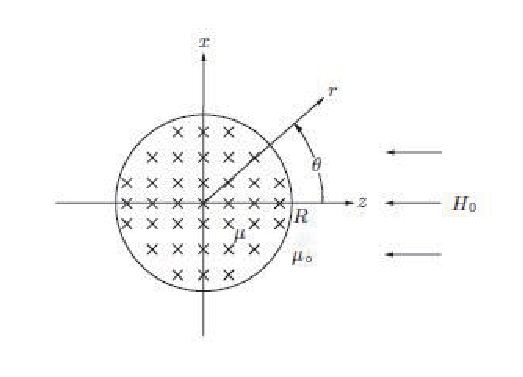
\includegraphics[scale=0.8]{chpt2/figs/fig2.1.eps}
  \caption{均匀场中的磁性球}
\end{figure}

\subsubsection*{问题2.1之解答}
a) 本题用标量势来解是最简单的。磁标量势表示为
$$\vec{H}=-\nabla \phi \eqno (S1.1)$$

对线性、各向同性介质,磁场和磁感应强度的关系为
$$\vec{B}=\mu \vec{H} \eqno (S1.2)$$

问题可以分为两个区域:区域1($r\ge R$)和区域2($r\le R$)。因为在$r=\infty$时,$H_\infty=H_0$,
在$r=0$时,$H\neq \pm \infty$,每个区域的标量势可选为:
	\begin{align}
\phi_1&=H_0 r\cos\theta+\frac{A}{r^2}\cos\theta \tag{S1.3a}\\
\phi_2&=C r \cos\theta \tag{S1.3b}
  	\end{align}

注意到,在$r\rightarrow \infty$时,$\phi_1\rightarrow H_0 r \cos\theta$;在$r=0$时,$\phi_2$是有限的。
应用$\nabla$算符,有:
	\begin{align}
\vec{H}_1&= H_0(−\cos\theta\vec{i_r} + \sin\theta\vec{i}_\theta) + \frac{A}{r^3}(2 \cos\theta\vec{i_r} + \sin\theta\vec{i_\theta})\tag{S1.4a}\\
\vec{H}_2&=C(-\cos\theta\vec{i_r} + \sin\theta\vec{i}_\theta) \tag{S1.4b}
  	\end{align}

\textbf{边界条件}

1)在$r=R$处,$\vec{H}$的切向分量连续,故无表面电流。这等价于在$r=R$时,有$\phi_1=\phi_2$:
$$H_0 + \frac{A}{R^3} = C \eqno (S1.5)$$

2)在$r=R$处,$\vec{B}$的法向连续:
$$\mu_0\left(-H_0 + 2\frac{A}{R^3} \right)= -\mu C \eqno (S1.6)$$

从S1.5和S1.6式,解出A和C两个常数:
$$C =\frac{3H_0\mu_0}{2\mu_0+\mu}\eqno (S1.7)$$
$$A=(C-H_0)R^3=H_0\left(\frac{\mu_0-\mu}{2\mu_0+\mu}\right)R^3 \eqno (S1.8)$$

于是,$\vec{B}_1$和$\vec{B}_2$可写为:
	\begin{align}
\vec{B}_1=& \mu_0 H_0(−\cos\theta\vec{i_r} + \sin\theta\vec{i_\theta}) \notag\\
&+\mu_0\left(\frac{\mu_0-\mu}{2\mu_0+\mu}\right)H_0\left(\frac{R}{r}\right)^3(2 \cos\theta\vec{i_r} + \sin\theta\vec{i_\theta})\tag{2.41a}\\
\vec{B}_2=&\frac{3\mu_0\mu H_0}{2\mu_0+\mu}(-\cos\theta\vec{i_r} + \sin\theta\vec{i_\theta}))\tag{2.41b}
  	\end{align}

下面,我们考虑三种$\mu/mu_0$的三种特例。

\textbf{特例1:$\mu/\mu_0=0$}

将$\mu=0$代入2.41式,可得

	\begin{align}
\vec{B}_1&= \mu_0 H_0(−\cos\theta\vec{i_r} + \sin\theta\vec{i_\theta}) +
\frac{\mu_0 H_0}{2}\left(\frac{R}{r}\right)^3 (2 \cos\theta\vec{i_r} + \sin\theta\vec{i_\theta})\tag{S1.9a}\\
\vec{B}_2&=0 \tag{S1.9b}
  	\end{align}

这个球像第I类超导体。球内不允许有磁通密度存在(Meissner效应)。问题2.2将会讨论到,$\vec{H}$在
$r=R$处的$\theta$分量不连续将要求存在表面电流(被限制在一个薄层内)。因为这个电流一旦建立起来,
会一直流下去,这就表明了球对电流是无电阻的。如第一章所言的,存在Meissner效应的材料必须同时是理想导体:
那这种材料其实就是超导体。

\textbf{特例2:$\mu/\mu_0=1$}

这时问题退化为平凡解,即等价于没有球的存在。代入方程2.41,两个方程将变成同一个。

\textbf{特例3:$\mu/\mu_0=\infty$}

这时表示的是一个理想铁磁材料。软铁的性质与此接近。磁场被“吸”如球内,代入2.41中,有
	\begin{align}
\vec{B}_1&= \mu_0 H_0(−\cos\theta\vec{i_r} + \sin\theta\vec{i_\theta}) -
\mu_0 H_0\left(\frac{R}{r}\right)^3 (2 \cos\theta\vec{i_r} + \sin\theta\vec{i_\theta})\tag{S1.10a}\\
\vec{B}_2&=3\mu_0 H_0(−\cos\theta\vec{i_r} + \sin\theta\vec{i_\theta})\tag{S1.10b}
  	\end{align}


可见,球内的磁感应强度是外施磁场的3倍。注意到,如果球存在磁化饱和,则$\mu$不再是$\infty$。所有磁性
材料都存在的磁场饱和效应将在问题4中讨论。

b) 图2.2给出了$\mu/\mu_0=0.1$和$\mu/\mu_0=100$两种情况下的磁场线。

\begin{figure}[htbp]
  \centering
 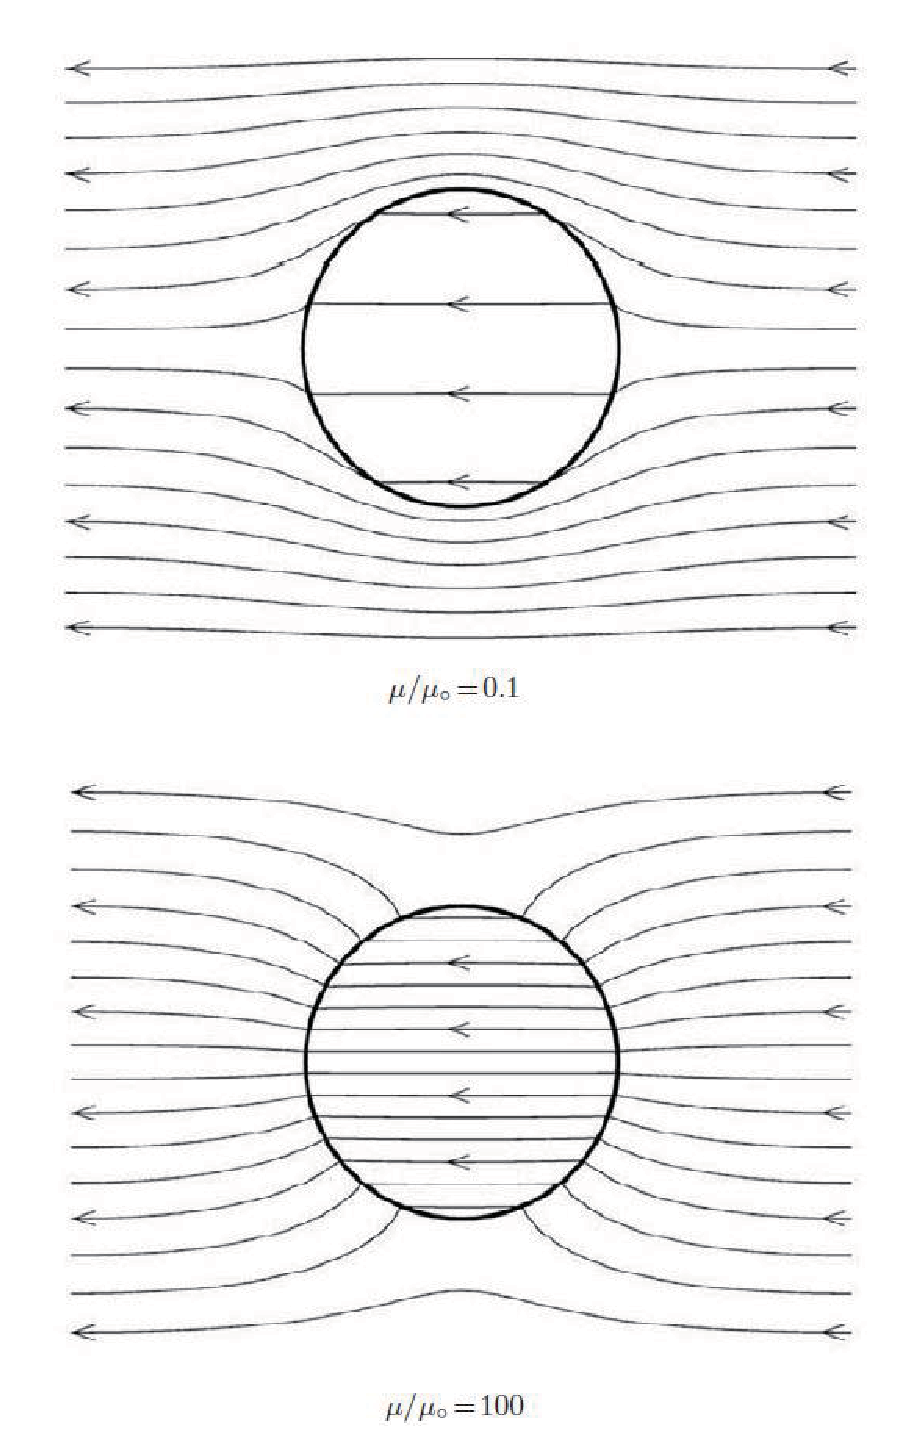
\includegraphics[scale=0.4]{chpt2/figs/fig2.2.eps}
  \caption{两种特例下球内和球附近的磁场线。上球在无穷远处的磁场线密度是球内的2.6倍;下球仅为1.7倍}
\end{figure}
\newpage


\subsection{问题2.2:均匀场中的第I类超导棒}
本题处理第I代超导体的Meissner效应,并用London超导理论对结果进行解释。
图2.3给出了无限长、圆截面(半径$R$)的Pb棒,置于垂直于轴向的均匀外磁场中。
\begin{equation*}\label{eqn:2.40}
  \vec{H}_\infty = H_0 (-\cos \theta\vec{i_r}+\sin\theta\vec{i_\theta}) \tag{2.40}
\end{equation*}

式中,$\mu_0H_0=0.08\ \mathrm{T}$。初始状态,棒处于正常态,于是磁场在棒的内外是处处相同的。棒逐步冷却至超导态。

a)证明在外磁场暂态效应消失后,棒外场的表达式为
\begin{equation}
  \vec{H}_1=H_0(-\cos\theta\vec{i_r}+\sin\theta\vec{i_\theta})+H_0\left(\frac{R}{r}\right)^2 (\cos\theta\vec{i_r}+\sin\theta\vec{i_\theta})
\end{equation}

b) 证明在穿透深度$\lambda\ll R$内的电流密度$K_f [\mathrm{A/m}]$的表达式为
\begin{equation}
  \vec{K}_f=2H_0 \sin\theta\vec{i_z}
\end{equation}

c)将表面电流密度幅值转换为(体)电流密度$J_f [\mathrm{A/m^2}]$。证明用London超导理论导出的电流密度值和这个值是一致的。

\begin{figure}[htbp]
	\centering
	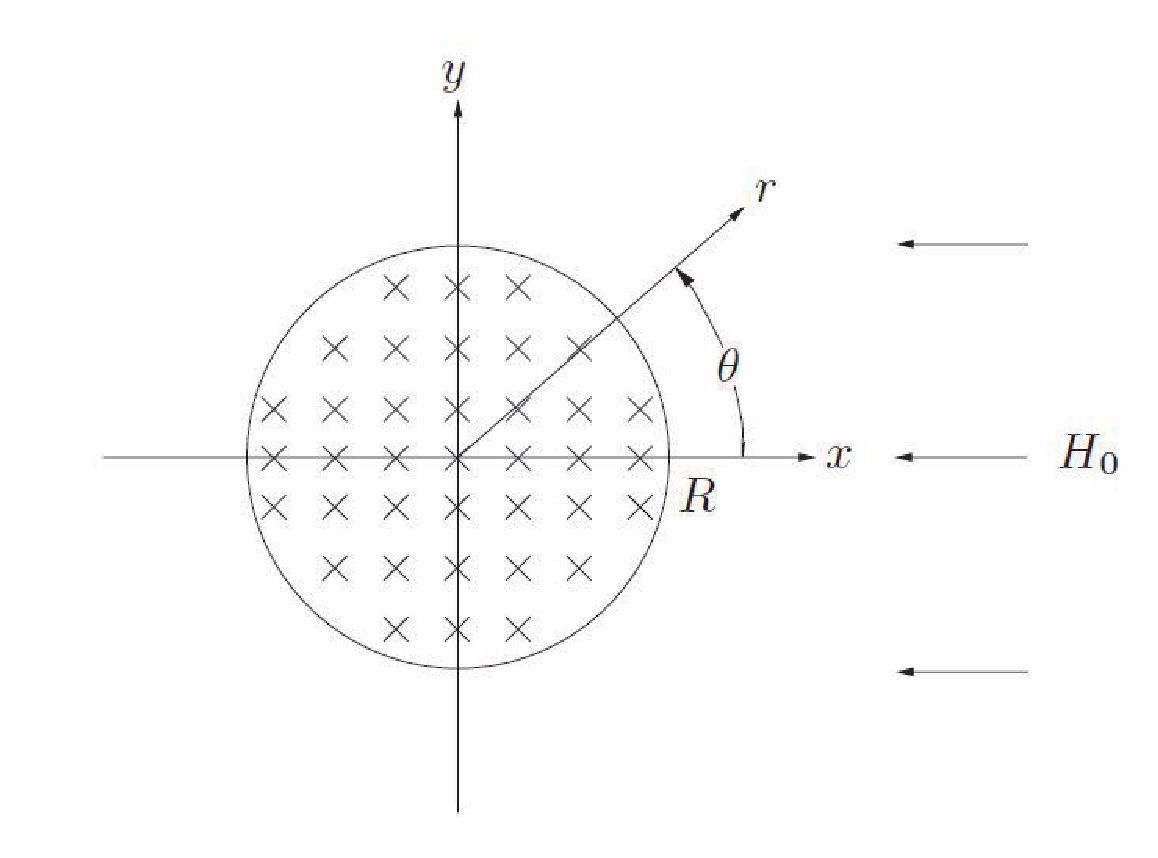
\includegraphics[scale=0.4]{chpt2/figs/fig2.3.eps}
	\caption{无限长、圆截面超导棒置于均匀磁场中。}
\end{figure}

\subsubsection*{问题2.2之解答}
a) 问题可以分为两个区域:区域1($r\ge R$)和区域2($r\le R$)。因为我们处理的是第I类超导体,也即圆棒超导时有$\vec{B}_2=0 (\phi_2=0)$。
区域1的场可由势函数导出:
$$  \phi_2=H_0 r \cos \theta +\frac{A}{r} \cos \theta \eqno(S2.1)$$
注意到,当$r\rightarrow \infty $时,$\phi_1\rightarrow H_0 r \cos\theta$。

在圆柱坐标系下使用$\nabla$算符,可以得到$\vec{H}$:
\begin{align}
\vec{H}_1=&-\frac{\partial}{\partial r}(H_0 r \cos\theta +\frac{A}{r}\cos\theta)\vec{i}_r-\frac{1}{r}\frac{\partial}{\partial \theta}(H_0 r \cos\theta +\frac{A}{r}\cos\theta)\vec{i}_\theta \tag{S2.2}\\
=&-(H_0 \cos\theta +\frac{A}{r^2}\cos\theta)\vec{i}_r-(-H_0 \sin\theta -\frac{A}{r^2}\sin\theta)\vec{i}_\theta \tag{S2.3}
\end{align}

整理S2.3式,可得
\begin{equation*}
\vec{H}_1=H_0(-\cos \theta \vec{i}_r+\sin \theta \vec{i}_\theta) +\frac{A}{r^2}(\cos\theta \vec{i}_r+\sin\theta \vec{i}_\theta )\tag{S2.4}
\end{equation*}

$B$法向分量的连续性要求S2.3中$\vec{i}_r$的系数在$r=R$处为零:
\begin{equation*}
-H_0+\frac{A}{R^2}=0  \tag{S2.5}
\end{equation*}

解出上式,得
\begin{equation*}
A=R^2 H_0 \tag{S2.6}
\end{equation*}

于是,超导圆棒外的场(区域1)可以写为:
\begin{equation*}
\vec{H}_1=H_0(-\cos \theta \vec{i}_r+\sin \theta \vec{i}_\theta) +H_0 \left(\frac{R}{r}\right)^2(\cos\theta \vec{i}_r+\sin\theta \vec{i}_\theta ) \tag{2.42}
\end{equation*}

注意到,在$r=R,\theta=90^\circ$时,$|\vec{H}_1|=2H_0$;也即此处的幅值是远场的两倍。物理上看,圆棒处于正常态时场本是在其内部的,进入超导态后,场被“推”出,挤压在$\theta=90^\circ$附近。


b) 因为$2H_0\sin \theta$中的$\vec{H}$在$r=R$处的切向分量不连续,所以肯定存在表面电流密度$\vec{K}_f$流过超导棒。我们有:

\begin{equation*}
  \vec{K}_f=\vec{i}_r \times 2H_0\sin\theta \vec{i}_\theta=2H_0\sin\theta\vec{i}_z\tag{2.43}
\end{equation*}

这个正弦电流分布式高能物理设施中被称为“核粒子加速器”内所用的大多数双极磁体的基础。


c) 根据超导电性的London理论,第I类超导体的超导电流密度$J_s$由$J_s=en_{se}v$给出。其中,$e$是电荷量($e=1.6\times 10^{-19}\ \mathrm{C}$),$n_{se}$是超导电子的密度,$v$是超导电子的漂移速度。
超导电子的密度\textbf{大致}上等于自由电子的密度:

\begin{equation*}
n_{se}\simeq n_{fe}=\frac{\rho N_A}{W_A} \tag{1.2}
\end{equation*}

对于铅,$\rho=11.4\ \mathrm{g/cm^3};N_A=6.023\times 10^{23};W_A=207.2\ \mathrm{g/mole}$,我们得到单位体积的电子数量:
\begin{equation*}
n_{se}=\frac{11.4\times 6.023\times 10^{23}}{207.2} \simeq 3.3\times 10^{28}\ \mathrm{electron/m^3} \tag{S2.7}
\end{equation*}

超导电子的漂移速度约为$200\ \mathrm{m/s}$,于是我们可以得到$J_s$的量级:
$$
J_s=e n_{se} v\sim 1.6\times 10^{-19} \times 3.3\times 10^{28} \times 200 \sim 1\times 10^{12}\ \mathrm{A/m^2} 
$$

在上述铅圆柱棒所要求的表面电流密度($K_f=J_f \lambda$)下,$J_f$应\textbf{大致}上与$J_s$相等,也即与上面所计算的$J_s$在同一个量级上。
London理论给出了供超导电流流过的超导体表面穿透深度$\lambda$的表达式:
\begin{equation*}
\lambda=\sqrt{\frac{m}{\mu_0 e^2 n_{se}}} \tag{1.1}
\end{equation*}

其中,$n_{se}$上面已经给出,$m=9.1\times 10^{-31}\ \mathrm{kg}$,则:
$$
\lambda=\sqrt{\frac{9.1\times 10^{-31}}{4\pi \times 10^{-7}\times 1.6\times 10^{-19}\times 3.3\times 10^{28}}}\simeq 3\times 10^{-8} m
$$

由于$K_f=J_f\lambda$,则
\begin{equation*}
J_f=\frac{2H_0}{\lambda}=\frac{2\mu_0 H_0}{\mu_0 \lambda}\simeq 4\times 10^{12} \ \mathrm{A/m^2}  \tag{S2.9}
\end{equation*}

也即,$J_f$与$J_s$\textbf{大致}上相等。
\newpage



\subsection{讨论2.1:均匀场中的理想导体球}
本题我们推导理想导体($\rho=0$)球置于磁场中的定量磁场表达。特别是针对图 1.1c中的$C\Rightarrow D$转变过程。
点C处,包括球内的整个空间处于均匀外场中(问题1,eq. 2.40)。外施场合问题1中的图 2.1相同。

当均匀外场降至$0$(图1.1c中的D点),由于球内的磁感应无法改变,其磁场$\vec{H_2}$必保持不变。远离球中心($r\rightarrow \infty$)处的外场$\vec{H_1}$为0。靠近球处的磁场可由标量势$\phi_1=(A/r^2)\cos\theta$导出。
在$\phi_1$上应用$\nabla$算符,可得到球坐标下的偶极场。
\begin{subequations}
	\begin{align}
\vec{H_2}=&H_0 (-\cos\theta \vec{i_r}+\sin\theta \vec{i_\theta})  \qquad(r\le R) \\
\vec{H_1}=&\frac{A}{r^3}(2\cos\theta \vec{i_r}+\sin\theta \vec{i_\theta})\qquad  (r\ge R)
	\end{align}
\end{subequations}

在$r=R$处,$B$的法向分量应连续。由于在$\theta=0$处球内外的磁场均仅有法向分量,故:
$$
-H_0=2\frac{A}{R^3}
$$

于是,$A=-H_0 R^3/2$,进而:
\begin{equation*}
\vec{H_1}=-H_0\left(\frac{R}{r}\right)^3 (\cos\theta \vec{i_r}+\frac{1}{2}\sin\theta \vec{i_\theta}) \tag{2.44c}
\end{equation*}


上式即磁场分布的定量表达。不同的是,图1.1c的外场是自下向上的,而图2.1的磁场是自右向左的。

在$r=R$处,磁场切向分量的不连续等于在$r=R$处球表面电流密度$\vec{K}_f$。联立方程2.6、2.44a和2.44c,有:
\begin{equation}
  \vec{K}_f=\vec{i_r}\times \left[H_0 \sin\theta \vec{i_\theta}-(-\frac{1}{2}H_0 \sin\theta \vec{i_\theta})\right]=\frac{3}{2}H_0\sin\theta\vec{i_\theta}
\end{equation}

值得一提的是,这个$\sin\theta$分布,可以用一个绕在球上的在$z$轴均匀匝密度的“薄”线圈来近似。
\newpage



\subsection{问题2.3:球壳的磁屏蔽}
本问题处理被动磁屏蔽。在MRI、磁悬浮等一些人和磁场敏感设备必须暴露于磁场外缘的高场系统中磁屏蔽是非常重要的课题。
美国食药局(FDA)规定,MRI中的最大外缘磁场为5高斯($0.5\ \mathrm{mT}$)。

在空间中的球星区域,屏蔽一个均匀磁场$\vec{H}_\infty$:
\begin{equation*}
\vec{H}_\infty=H_0 (-\cos\theta \vec{i_r}+\sin\theta \vec{i_\theta})\tag{2.40}
\end{equation*}

为了形成屏蔽,可以用一个外径为$2R$、壁厚$d/R\ll 1$、高磁导率材料($\mu/\mu_0 \gg 1$)的球壳,如图2.4所示。

a) 将本问题视为均匀外磁场中的磁性球壳。证明$H_{ss}/H_0$有如下表达式。其中,$H_{ss}$为球壳内($r\le R-d$)的磁场幅值
\begin{equation}
\frac{H_{ss}}{H_0}=\frac{9\mu_0 \mu}{9\mu_0 \mu+2(\mu-\mu_0)^2\left[1-\left(1-\frac{d}{R}\right)^3\right]}
\end{equation}

b)证明,在极限情况$\mu/\mu_0\gg 1$和$d/R\ll 1$下,$H_{ss}/H_0$可约化为
\begin{equation}
\frac{H_{ss}}{H_0}\simeq \frac{3}{2}(\frac{\mu_0}{\mu})(\frac{R}{d})
\end{equation}

c)用微扰法得到上式。首先,在$\mu=\infty$条件下解出壳上($R-d\le r\le R$)的磁场。接着,用微扰法在$\mu/\mu_0 \gg 1$条件下得到上式。

d)实践中,屏蔽材料中的磁通必须控制在材料的饱和磁通($\mu_0 M_{sa}$)之下。证明,可保持壳不饱和的$d/R$表达式为
\begin{equation}
\frac{d}{R} \ge \frac{3H_0}{2M_{sa}}
\end{equation}

e)画出$\mu/\mu_0 \gg 1$情况下的场线。

\begin{figure}[htbp]
  \centering
 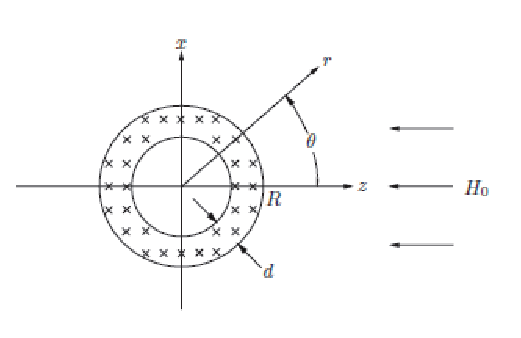
\includegraphics[scale=0.9]{chpt2/figs/fig2.4.eps}
  \caption{均匀磁场中的磁性球壳}
\end{figure}

\subsubsection*{问题2.3之解答}
a)问题可以分为三个区域:区域1($r\ge R$);区域2(球壳);区域3($r\le R-d$)。相应的势函数为:
\begin{align}
  \phi_1 =& H_0 r\cos\theta+\frac{A}{r^2}\cos\theta \tag{S3.1a} \\
  \phi_2 =& C r \cos\theta+\frac{D}{r^2}\cos\theta\tag{S3.1b} \\
  \phi_3 =& H_{ss} r\cos\theta  \tag{S3.1c}
\end{align}

注意到,在$r\rightarrow \infty$时,$\phi_1 \rightarrow H_0 r\cos\theta$以及在$r\rightarrow 0$时,$\phi_3$为有限值。应用球坐标下的$\nabla$算符,得到
\begin{align}
  \vec{H}_1 =& H_0 (-\cos\theta\vec{i_r}+\sin\theta\vec{i}_\theta)+\frac{A}{r^3} (2\cos\theta\vec{i_r}+\sin\theta\vec{i}_\theta) \tag{S3.2a}\\
  \vec{H}_2 =& C(-\cos\theta\vec{i_r}+\sin\theta\vec{i}_\theta)+\frac{D}{r^3} (2\cos\theta\vec{i_r}+\sin\theta\vec{i}_\theta)  \tag{S3.2b}\\
   \vec{H}_3 =& H_{ss}  (-\cos\theta\vec{i_r}+\sin\theta\vec{i}_\theta)  \tag{S3.2c}
\end{align}

\textbf{边界条件:}

\begin{enumerate}
  \item $r=R$处,$\vec{H}$的切向分量$H_\theta$连续:$\phi_1=\phi_2   $
  \item 类似的,在$r=R-d$处,$H_\theta$连续:$\phi_2=\phi_3  $
  \item 在$r=R$处,$\vec{B}$的法向分量$B_r$连续
  \item 类似的,在$r=R-d$处,$B_r$连续
\end{enumerate}

由上述边界条件,可导出下面的四个方程:
\begin{align}
  H_0+\frac{A}{R^3}=& C+\frac{D}{R^3} \nonumber \tag{S3.3a}\\
  C+\frac{D}{(R-d)^3}=& H_{ss} \nonumber \tag{S3.3b}\\
  \mu_0(-H_0+\frac{2A}{R^3})=& \mu\left(-C+\frac{2D}{R^3}\right)\nonumber \tag{S3.3c} \\
  \mu\left[-C+\frac{2D}{(R-d)^3}\right]=& -\mu_0 H_{ss} \nonumber\tag{S3.3d}
\end{align}

联立S3.3a和S3.3b,消去$C$:
\begin{equation*}
\frac{A}{R^3}+D\left[\frac{1}{(R-d)^3}-\frac{1}{R^3}\right]-H_{ss} =-H_0 \tag{S3.4}
\end{equation*}


联立S3.3b和S3.3d,解出$D$:
\begin{equation*}
D=\frac{\mu-\mu_0}{2\mu} (R-d)^3 H_{ss}  \tag{S3.5}
\end{equation*}

于是,可以$H_{ss}$表示$A/R^3$:
\begin{equation*}
\frac{A}{R^3}=H_{ss}\left\{1-\frac{\mu-\mu_0}{3\mu}\left[1-\left(1-\frac{d}{R}\right)^3\right]\right\}-H_0   \tag{S3.6}
\end{equation*}

联立S3.3c和S3.3d,得到:
\begin{equation*}
\frac{2A}{R^3}+2\frac{\mu}{\mu_0}D\left[\frac{1}{(R-d)^3}-\frac{1}{R^3}\right]+H_ss =H_0  \tag{S3.7}
\end{equation*}

联立S3.3-S3.7,用$H_0$表达$H_{ss}$,可以得到:
\begin{equation*}
\frac{H_{ss}}{H_0}=\frac{9\mu_0 \mu}{9\mu_0 \mu+2(\mu-\mu_0)^2\left[1-\left(1-\frac{d}{R}\right)^3\right]}  \tag{2.46}
\end{equation*}

b) 方程右侧的分子分母同除$\mu_0^2$,应用极限$\mu/\mu_0\gg 1$和$d/R\ll 1$:
\begin{align}
\frac{H_{ss}}{H_0}\simeq& \frac{9\mu/\mu_0}{9\frac{\mu}{\mu_0}+2(\frac{\mu}{\mu_0})^2\left[1-(1-3\frac{d}{R})\right]} \nonumber\tag{S3.8}\\
\simeq&\frac{3}{3+2(\frac{\mu}{\mu_0})(\frac{d}{R})}\nonumber \tag{S3.9}
\end{align}

在$\mu d/\mu_0 R \gg 1$的特殊情况下,S3.9可以简化为:
\begin{equation*}
\frac{H_{ss}}{H_0}\simeq \frac{2}{3}(\frac{\mu_0}{\mu})(\frac{R}{d})  \tag{2.47}
\end{equation*}

c)我们假设$\mu$为无限大。这要求B线在$r=R$处垂直于球壳。这是因为在$r=R$处,$\vec{H}_1$仅有径向分量。由于壳内$H=0$,故在$r=R$处$H_\theta$必须连续。
注意到,当$\mu=\infty$时,$C=D=0$。这样,$A=-R^3 H_0$,于是在$r=R$处
\begin{equation*}
\vec{H}_1=-3 H_0 \cos\theta \vec{i_r} \tag{S3.10}
\end{equation*}

\begin{figure}[htbp]
	\centering
	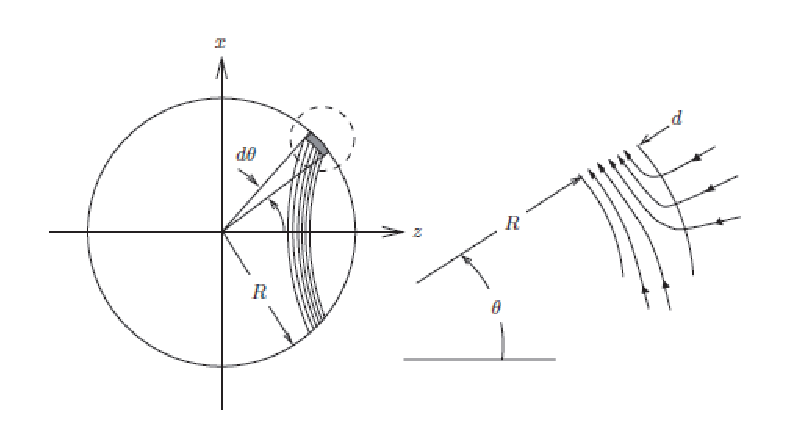
\includegraphics[scale=0.7]{chpt2/figs/fig2.5.eps}
	\caption{通过球壳$\pm \theta$边界内区域进入壳的磁通。}
\end{figure}

B线局限在壳内,不会“逸”至区域3。也即,壳内的B仅有$\vec{i}_\theta$分量。应用磁通连续性($\nabla \cdot \vec{B}=0$)并在$\mu=\infty$条件下解$B_2$。解出$B_2$
后,可以得到$\mu \neq \infty$但$\mu/\mu_0 \gg 1$时$\vec{H}_3$的近似表达式。

首先,计算通过表面区域$\pm \theta$边界内进入壳的总磁通(图2.5)。根据图中的微元积分
\begin{align}
\Phi=&\mu_0\int_{0}^{\theta} \vec{H}_1 \cdot d\vec{A}=\mu_0\int_{0}^{\theta} 3H_0\cos\theta 2\pi R^2 \sin\theta d\theta\nonumber\\
=&3\pi\mu_0 R^2 H_0 \sin^2 \theta\nonumber \tag{S3.11}
\end{align}


这个$\Phi$一定等于在球壳$\theta$处$\theta$方向的磁通量。
在$d\ll R$条件下,壳在$\theta$处的截面区域$A_2$可由下式给出
\begin{equation*}
A_2\simeq d\cdot 2\pi R\sin\theta \tag{S3.12}
\end{equation*}

我们有
\begin{align}
\Phi=&3\pi\mu_0 R^2 H_0 \sin^2 \theta\nonumber\\
\simeq& B_2 A_2=B_2 d 2 \pi R \sin\theta \tag{S3.13}
\end{align}

解出$B_2$,得
\begin{equation*}
\vec{B}_2\simeq \frac{3}{2}\mu_0 \left(\frac{R}{d}\right) H_0\sin\theta\vec{i}_\theta \tag{S3.14}
\end{equation*}

注意到上式的$\vec{B}_2$是在$\mu=\infty$条件下得到的。现在我们可以导出$\vec{H}_3$的近似表达。
由于$\vec{H}$的$\vec{i}_\theta$分量在$r=R-d$处必须连续,于是
\begin{equation*}
H_{\theta 3}\simeq \frac{B_{\theta 2}}{\mu}=\frac{3}{2}\left(\frac{\mu_0}{\mu}\right)\left(\frac{R}{d}\right)H_0\sin\theta \tag{S3.15}
\end{equation*}

得到了$H_{\theta 3}$,我们就可以给出$\vec{H}_3$的完整表达式了:
\begin{align}
\vec{H}_3\simeq \frac{B_{\theta 2}}{\mu}=&\frac{3}{2}\left(\frac{\mu_0}{\mu}\right)\left(\frac{R}{d}\right)H_0(-\cos\theta\vec{i_r}+\sin\theta\vec{i}_\theta) \nonumber\tag{S3.16a}\\
\left|\frac{\vec{H}_3}{H_0}\right|\simeq& \frac{3}{2}\left(\frac{\mu_0}{\mu}\right)\left(\frac{R}{d}\right) \nonumber\tag{S3.16b}
\end{align}

方程S3.16b给出的比值与方程2.47给出的$H_{ss}/H_0$是一致的。
注意:此处的微扰法需要$\mu=\infty$和$d\ll R$条件,但无需$\mu d/\mu_0 R \gg 1$条件。

d)应当明确,不能为了满足$d/R \ll 1$而将$d$选的特别小。事实上,下面的分析仅在下式条件满足时有效:
\begin{equation*}
\frac{\mu_0}{\mu} \ll \frac{d}{R} \ll 1 \tag{S3.17}
\end{equation*}

实际的$\mu$不可能无限大。屏蔽材料会随着外场的增大最终饱和。因此,壳内的最大磁通($\theta=90^\circ$时取得)必须小于屏蔽壳材料的饱和磁通$\mu_0 M_{sa}$。
于是
\begin{equation*}
\frac{3}{2}\left(\frac{R}{d}\right)\mu_0 H_0 \le \mu_0 M_{sa}  \tag{S3.18}
\end{equation*}

在S3.18中解出$d/R$,有
\begin{equation*}
\frac{d}{R}\gg \frac{3H_0}{2M_{sa}}  \tag{2.48}
\end{equation*}

表\ref{my-label} 给出了三种材料的微分$\mu/\mu_0$和$\mu_0M(H_0)$的近似值。其中,$(\mu/\mu_0)_{dif}\equiv \Delta M/ \Delta H_0 |_{\mu_0 H_0}$,$\mu_0 H_0$的范围为$0\sim 1000$高斯。
后面还给出了这三种材料的饱和磁通值。这几种材料常用来屏蔽$\sim 100$高斯下的磁场。

\begin{table}[]
\centering
\caption{几种材料的屏蔽特征值}
\label{my-label}
\begin{tabular}{|c|c|c|c|c|c|c|}
\hline
\multirow{2}{*}{$\mu_0 H_0$[gauss]} & \multicolumn{2}{c|}{annealed ingot iron} & \multicolumn{2}{c|}{As-Cast Steel} & \multicolumn{2}{c|}{Vanadium Permendur} \\ \cline{2-7}
                                  &$ (\mu/\mu_0)_{dif} $      & $\mu_0 $M[T]  & $(\mu/\mu_0)_{dif}   $ &$ \mu_0 M$[T]   &$ (\mu/\mu_0)_{dif}    $  & $\mu_0 M$[T]      \\ \hline
1                                 & 7710                   & 0.375           & na                  & na           & na                    & na              \\ \hline
3                                 & 3850                   & 0.91            & 1660                & 0.25         & 4845                  & 0.65            \\ \hline
5                                 & 500                    & 1.42            & 1155                & 0.51         & 1875                  & 1.25            \\ \hline
10                                & 115                    & 1.54            & 565                 & 0.93         & 545                   & 1.67            \\ \hline
20                                & 47                     & 1.60            & 180                 & 1.25         & 170                   & 1.96            \\ \hline
50                                & 23.5                   & 1.70            & 50                  & 1.52         & 17                    & 2.10            \\ \hline
100                               & 17.5                   & 1.81            & 25                  & 1.70         & 4.8                   & 2.15            \\ \hline
200                               & 8.25                   & 1.93            & 10                  & 1.85         & 1.3                   & 2.17            \\ \hline
500                               & 2.0                    & 2.05            & 1.0                 & 1.92         & 0.26                  & 2.18            \\ \hline
1000                              & 0.4                    & 2.11            & 0.45                & 2.01         & 0.07                  & 2.19            \\ \hline
$\mu_0 M_{sa} $                     & \multicolumn{2}{c|}{2.13[T]}             & \multicolumn{2}{c|}{2.03[T]}       & \multicolumn{2}{c|}{2.20[T]}            \\ \hline
\end{tabular}
\end{table}

e) $\mu/\mu_0=100$磁性球壳置于均匀场中的磁场分布如图2.6所示。

\begin{figure}
  \centering
 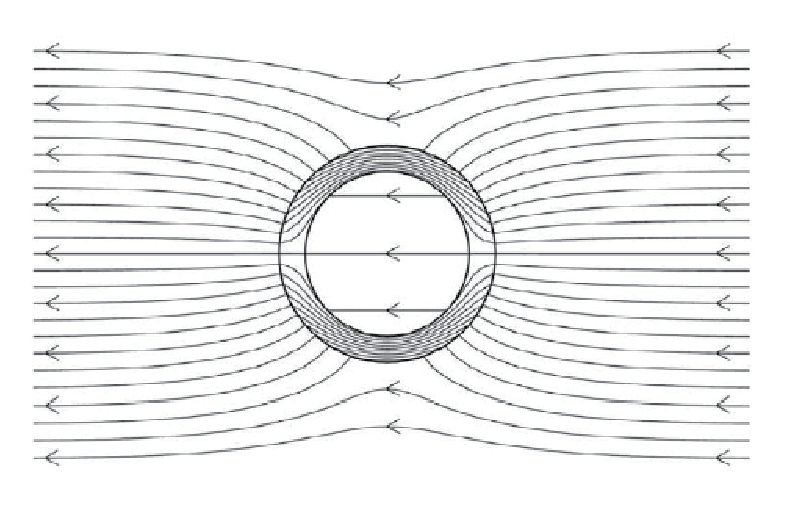
\includegraphics[scale=0.7]{chpt2/figs/fig2.6.eps}
  \caption{$\mu/\mu_0=100$磁性球壳置于均匀场中的磁场分布。注意到进出球壳的磁场线是近乎垂直于壳的。}
\end{figure}
\newpage


\subsection{讨论2.2:用圆柱壳屏蔽}
我们用类似于问题4中所用的微扰技术推导$H_{cs}/H_0$的表达式。式中,$H_{cs}$是置于均匀外场采用高磁导率($\mu/\mu_0 \gg 1$)材料的圆柱壳($d/R\ll 1$)内部($r\le R-d$)的磁场的幅值。
在二维柱坐标系下,外场有如下形式:
\begin{equation*}
\vec{H}_\infty =H_0 (-\cos\theta \vec{i_r}+\sin\theta\vec{i}_\theta) \tag{2.40}
\end{equation*}


我们假定圆柱材料的$\mu$是无限大的,这样B线在$r=R$处必须垂直于圆柱。于是,在$r=R$处,有
$$\vec{H}_1 =-2 H_0 \cos\theta \vec{i_r}$$

当然,壳内的B是$\theta$方向的。在$d/R\ll 1$条件下,磁通连续性要求B满足:
$$B_2 d=\int_{0}^{\theta}2\mu_0 H_0 R\cos\theta d\theta=2\mu_0 R H_0 \sin\theta$$

于是,
$$\vec{B}_2=2\mu_0 (\frac{R}{d})H_0 \sin\theta \vec{i}_\theta$$

已知$\mu=\infty$下的$\vec{B}_2$,我们可以得到$\mu/\mu_0 \gg 1$下的$\vec{H}_2$:
$$\vec{H}_2= \frac{\vec{B}_2}{\mu}\simeq 2(\frac{\mu_0}{\mu}) (\frac{R}{d})H_0 \sin\theta \vec{i}_\theta$$

因为在没有表面电流时$H_\theta$是连续的,区域2和区域3一定有$H_{\theta 2}=H_{\theta 3}$。于是,在$r=R-d$处:
$$H_{\theta 3}=H_{\theta 2}\simeq 2(\frac{\mu_0}{\mu}) (\frac{R}{d})H_0 \sin\theta$$

从上面的表达式,可以得出:
\begin{align}
\vec{H}_3 \simeq& 2(\frac{\mu_0}{\mu}) (\frac{R}{d})H_0 (-\cos\theta \vec{i_r}+\sin\theta\vec{i}_\theta)\nonumber\\
\left|\frac{\vec{H}_3}{H_0}\right|\equiv&\frac{H_{cs}}{H_0}\simeq 2(\frac{\mu_0}{\mu}) (\frac{R}{d})
\end{align}

如问题2.3中的球壳一样,圆柱壳的厚度也不能无线薄。它必须有保持足够的厚度以防止饱和:
$$\mu H_{cs}=2\mu_0 H_0 \frac{R}{d}\le \mu_0 M_{sa}$$

根据上面的推导,我们得到:
\begin{equation}
\frac{d}{R}\ge \frac{2H_0}{M_{sa}}
\end{equation}
\newpage


\subsection{问题2.4:四个偶极子簇的远场}
本题讨论如下图布置的四个理想偶极子簇的远场。各偶极子的方向如图箭头所示。两个相反偶极子的中心距为$2\delta_d$。各偶极子j均为零绕组厚度,直径均为$2r_d$,在y向的总长度为$l_d$,距离偶极子径向($r_j$)位置的远场($r_j \gg l_d$)可建模为球偶极子场$\vec{B}_j$:
\begin{equation}
\vec{B}_j=\frac{r_d^2 l_d B_0}{2r_j^3}(\cos\theta_j \vec{i}_{r_j}+\frac{1}{2} \sin\theta_j \vec{i}_{\theta_j})
\end{equation}

式中,$r_j$是分别到各偶极子中心的距离;$\theta_j$的定义确保$\theta_j=0^\circ$时,各偶极子的绕组内场指向$r_j$方向。图2.7给出了各偶极子内场的方向,还定义了对所有偶极子共同的$r-\theta$坐标系和$z-x$坐标系。注意到,$r\gg \delta_d$,我们有$\mathscr{\theta}_1=\theta+180^\circ,\theta_2=\theta-90^\circ,\theta_3=\theta,\theta_4=\theta + 90^\circ$。

证明,忽略各偶极子的末端效应,仅考虑$y=0$平面,本组合系统的远场($r/\delta_d \gg 1$)近似表达式为:
\begin{equation}
\vec{B}\simeq \frac{3r_d^2 l_d B_0 \delta_d}{r^4}(-\sin 2\theta \vec{i}_r+\frac{1}{2}\cos 2\theta \vec{i}_\theta)
\end{equation}

\begin{figure}[htbp]
  \centering
 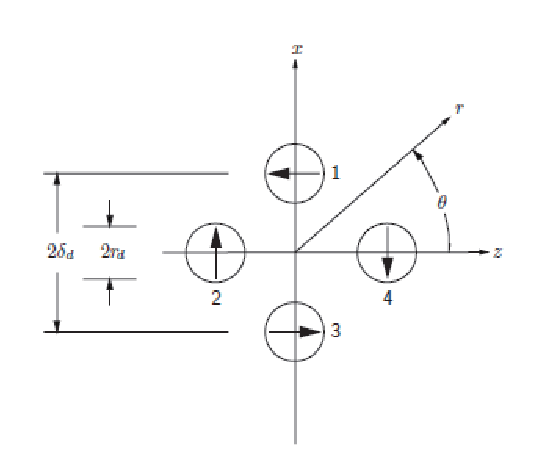
\includegraphics[scale=0.8]{chpt2/figs/fig2.7.eps}
  \caption{四个偶极子布置的横截面。每个偶极子的箭头指示线圈内场的方向。}
\end{figure}


\subsubsection*{问题2.4之解}
对于$r\gg \delta_d$,每个偶极子的$r_j$可以用$r$和$\theta$表示:
\begin{align}
r_1\simeq& r-\delta_d \sin\theta \nonumber\tag{S4.1a}\\
r_2\simeq& r+\delta_d \cos\theta\nonumber\tag{S4.1b}\\
r_3\simeq& r+\delta_d \sin\theta\nonumber\tag{S4.1c}\\
r_4\simeq& r-\delta_d \cos\theta\nonumber\tag{S4.1d}
\end{align}

由此,可以得到各偶极子采用$\theta$表示的场:
\begin{align}
\vec{B}_1 \simeq& \frac{r_d^2 l_d B_0}{2(r-\delta_d\sin\theta)^3}(-\cos\theta \vec{i}_r-\frac{1}{2}\sin\theta \vec{i}_\theta) \nonumber\tag{S4.2a}\\
\vec{B}_2 \simeq& \frac{r_d^2 l_d B_0}{2(r+\delta_d\cos\theta)^3}(\sin\theta \vec{i}_r-\frac{1}{2}\cos\theta \vec{i}_\theta)  \nonumber\tag{S4.2b}\\
\vec{B}_3 \simeq& \frac{r_d^2 l_d B_0}{2(r+\delta_d\sin\theta)^3}(\cos\theta \vec{i}_r+\frac{1}{2}\sin\theta \vec{i}_\theta) \nonumber\tag{S4.2c}\\
\vec{B}_4 \simeq& \frac{r_d^2 l_d B_0}{2(r-\delta_d\cos\theta)^3}(-\sin\theta \vec{i}_r+\frac{1}{2}\cos\theta \vec{i}_\theta)  \nonumber\tag{S4.2d}
\end{align}

对于$r\gg \delta_d$,各项的分母可对$\delta_d/r$作一阶展开,成为:
\begin{align}
\vec{B}_1 \simeq& \frac{r_d^2 l_d B_0}{2 r^3}\left[1+3(\frac{\delta_d}{r})\sin\theta \right](-\cos\theta \vec{i}_r-\frac{1}{2}\sin\theta \vec{i}_\theta)\nonumber\tag{S4.3a}\\
\vec{B}_2 \simeq& \frac{r_d^2 l_d B_0}{2 r^3}\left[1-3(\frac{\delta_d}{r})\cos\theta \right](\sin\theta \vec{i}_r-\frac{1}{2}\cos\theta \vec{i}_\theta)\nonumber\tag{S4.3b}\\
\vec{B}_3 \simeq& \frac{r_d^2 l_d B_0}{2 r^3}\left[1-3(\frac{\delta_d}{r})\sin\theta \right](\cos\theta \vec{i}_r+\frac{1}{2}\sin\theta \vec{i}_\theta)\nonumber\tag{S4.3c}\\
\vec{B}_4 \simeq& \frac{r_d^2 l_d B_0}{2 r^3}\left[1+3(\frac{\delta_d}{r})\sin\theta \right](-\sin\theta \vec{i}_r+\frac{1}{2}\cos\theta \vec{i}_\theta)\nonumber\tag{S4.3d}
\end{align}

组合上面几式,可以得到
\begin{equation*}
\vec{B}=\vec{B}_1+\vec{B}_2+\vec{B}_3+\vec{B}_4\simeq \frac{3r_d^2 l_d B_0 \delta_d}{r^4}(-\sin 2\theta \vec{i}_r+\frac{1}{2}\cos 2\theta \vec{i}_\theta) \tag{2.52}
\end{equation*}

注意到,四偶极子簇的$|B|$按$\propto 1/r^4$衰减而不是像单个偶极子一样的依照$\propto 1/r^3$衰减。
\newpage



\subsection{问题2.5:铁电磁体的磁极形状}
图2.8给出了铁制电磁铁的剖面。两个铁磁材料制成的圆柱形磁极相对放置,圆柱尖端倒角成锥形(图中的阴影部分)。
磁极上的线圈(图中未画出)通电后,两极间的间隙内将产生一个相对均匀的磁场。
中心场理论上没有上限,因为它是$\propto \ln(R_2/R_1)$增长的。其中,$R_1$和$R_2$分别是锥体顶部和基部的直径。
由于随着$R_2$增加,磁体的质量会变得很大,所以实践中的中心场上限$\sim 7\ \mathrm{T}$(巴黎Bellevue;瑞典Uppsala Uni.)。
由于尖端部分的磁矩产生的场对中心的z向场有一个负的贡献,所以,尖角能够加强中心场。

证明:若铁芯在与系统z轴平行方向励磁,$\theta_{tp}=54^\circ 44^\prime$是这种简单磁极几何的最优角度。
假定中心场是均匀分布于磁极件上的磁矩产生的场的叠加。$z$向励磁的磁矩$\vec{m}_A [\mathrm{A\cdot m^2}]$产生的偶极场为:
\begin{equation}
\vec{H}_{m_A}=\frac{\vec{m_A}}{r^3}(\cos\theta \vec{i}_r+\frac{1}{2}\sin\theta\vec{i}_\theta)
\end{equation}

$\vec{H}_{m_A}(r,\theta)$关于z轴对称,可以从标量势$\cos\theta/r^2$导出。

提示:解出位于磁极倒角基部边缘上(图示)的单个磁矩$m_A \uparrow$在z轴中心的场。

\subsubsection*{问题2.5的解}
$m_A$产生的在中心的场的z向分量$H_{m_A z}$为:
\begin{equation*}
H_{m_A z}=\frac{\vec{m_A}}{r^3}(\cos^2\theta-\frac{1}{2}\sin^2\theta) \tag{S5.1}
\end{equation*}

式中,$r_A$是$m_A$距中心的距离。在$\theta=\theta_{tp}$时,上述方程的右侧为0。于是
\begin{equation*}
\cos^2\theta_{tp}-\frac{1}{2}\sin^2\theta_{tp}=0 \tag{S5.2}
\end{equation*}

于是有$\cos\theta_{tp}=1/\sqrt{3}$或$\tan\theta_{tp}=\sqrt{2}$,也即$\theta_{tp}\simeq 54.736^\circ\simeq54^\circ 44^\prime$。

我们注意到,对阴影区中基线之上的磁矩均有$\theta_{tp}>54^\circ 44^\prime$。由于随$\theta$值的增加,$\cos\theta$递减而$\sin\theta$递增,
在$\theta_{tp}>54^\circ 44^\prime$时,$H_{m_A z}$为负。以$\theta_{tp}=54^\circ 44^\prime$倒角磁极可以消除这种负的贡献,最大化中心场。

值得一提的是,NMR质谱仪中的“神奇角”(magic angle)也是$54^\circ 44^\prime$。通常,NMR样品以这个“神奇角”与主轴场取向放置以减少各向异性的作用。

\begin{figure}[htbp]
  \centering
 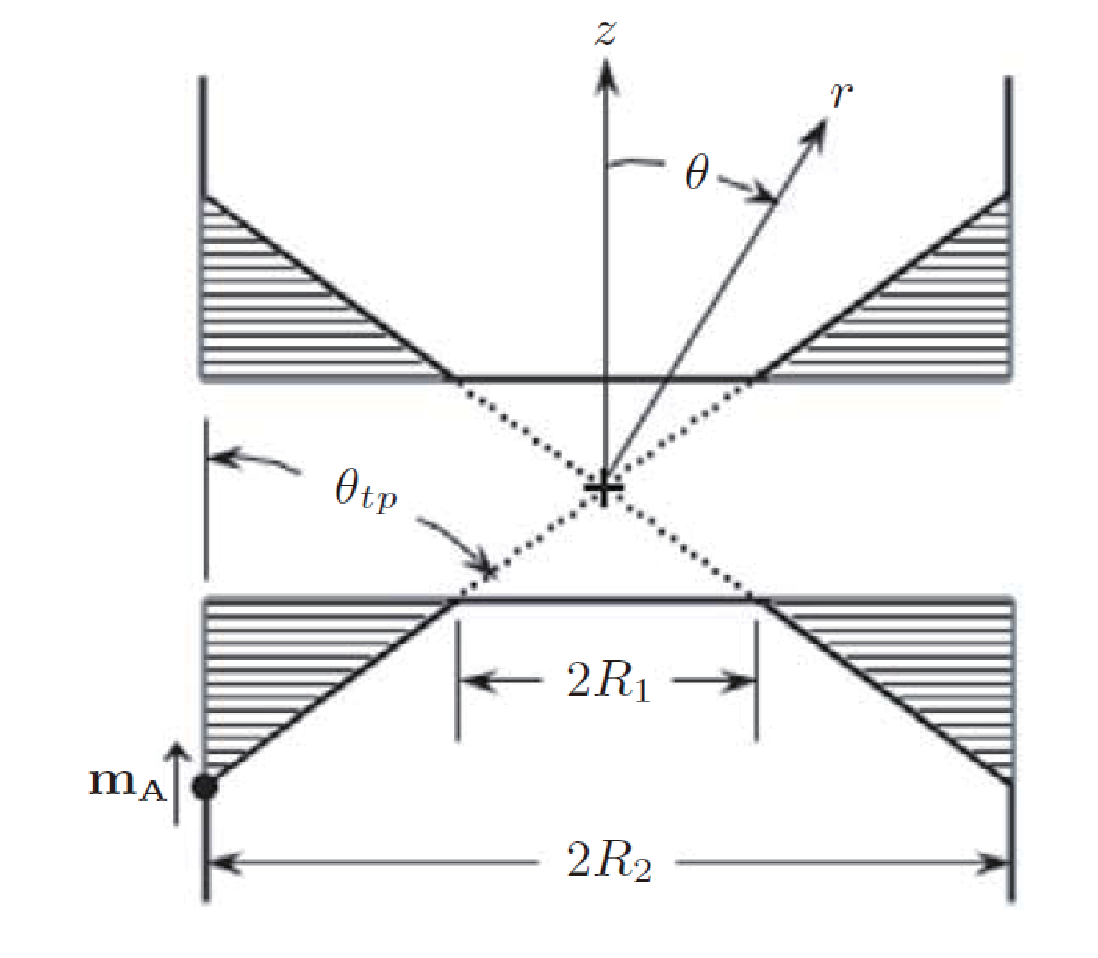
\includegraphics[scale=0.3]{chpt2/figs/fig2.8.eps}
  \caption{电极对,倒角为$\theta_{tp}$。图中$\bullet$指示了磁矩$\vec{m_A}\uparrow$的位置。}
\end{figure}
\newpage



\subsection{讨论2.3:永磁体}
永磁磁体是日常生活中大量设备如汽车、电视、电脑、手机、冰箱等的关键部件。实际上,如果没有永磁体,今日的现代生活将难以存续。
在低场($<1$)T的MRI中,永磁体是超导体的竞争对手。由于永磁磁体既无需制冷也很便宜,永磁MRI很受欢迎。

表2.6给出了90年(1910s-1990s)间永磁体和超导体的发展。永磁体性能以最大磁能$BH|_{mx}$表示,而超导体以最高临界温度$T_c|_{mx}$表示。
这期间,$BH|_{mx}$提高了约30倍,$T_c|_{mx}$提高了约20倍。

永磁体照这个步调发展下去,在不久的将来,永磁体MRI将能达到$\sim 1\ $T。
在这个磁场之上,还是超导的天下。

\begin{table}[htbp]
\centering
\caption{永磁体和超导体的发展历程}
\label{磁体和超导体的发展}
\begin{tabular}{|c|c|c|c|c|}
\hline
年代        & 永磁体 & $BH|_{mx}$[$\mathrm{kJ/m^3}$] & 超导体 & $T_c|_{mx}$[K]   \\ \hline
1910      &  特种钢   & 11       &  Pb   & 7.2 \\ \hline
1920-1940 &  Alnico 1-4   & 15       &   NbN  & 16  \\ \hline
1950      &   Alnico 5  & 35       &    $Nb_3 Sn$ & 18  \\ \hline
1960      &   Alnico 8,9  & 55       &   $Nb_{12}Al_3 Ge$  &   19  \\ \hline
1970      &   $SmCo_5 $  & 140      &  $Nb_3Ge$   & 23    \\ \hline
1980      &   $Sm(CoCuFeZr)  $& 240      &  $Bi_2 Sr_2 Ca_2 Cu_3 O_x$   & 118 \\ \hline
1990      &  $Nd_2Fe_{14}B$   & 350      & $(Hg, Pb) Sr_2 Ca_2 Cu_3 O_x$    & 133 \\ \hline
\end{tabular}
\end{table}
\newpage


\subsection{问题2.6:圆柱中的准静态场}
半径为R的长薄圆柱由理想导体($\rho=\infty$,非超导)薄板制成,侧面开有宽$\delta$的窄缝(如图)。
圆柱置于正弦时变磁场中:
\begin{equation}
\vec{H}_\infty(t)=Re[H_0 e^{j\omega t}] \vec{i}_z
\end{equation}

式中,$H_0$是复幅值。忽略端部效应。

a)忽略$\delta/R$阶项。证明:跨窄缝短边的一阶复电压幅值为:
\begin{equation}
V_{1|0}\equiv V_{1|\theta=0}=-j\omega \pi R^2 \mu_0 H_0
\end{equation}

b)一个电阻率为$\rho[\Omega\cdot m]$的正常金属板置于窄缝将圆柱开缝恰好连接起来。推导通过该板的一阶复电流密度(轴向单位长度)$J_1 [\mathrm{A/m}]$的表达式。
假定:驱动频率($\omega/2\pi$)足够小,磁场仍保持原准静态形式;电流在板截面上均匀流过。

c)在无金属板存在(或$\rho_s=\infty$)条件下,在圆柱腔内画出6条一阶复电场矢量($\vec{E}_1$)线,指明电场的重要特征。

d)在无金属板存在条件下,推导两点间的一阶电压的线积分$V_1 |_{\theta=-\pi/2}^{\theta=+\pi/2}$的表达式,即一点位于$\theta=+\pi/2$,另一点位于$\theta=-\pi/2$。

\begin{figure}[htbp]
  \centering
 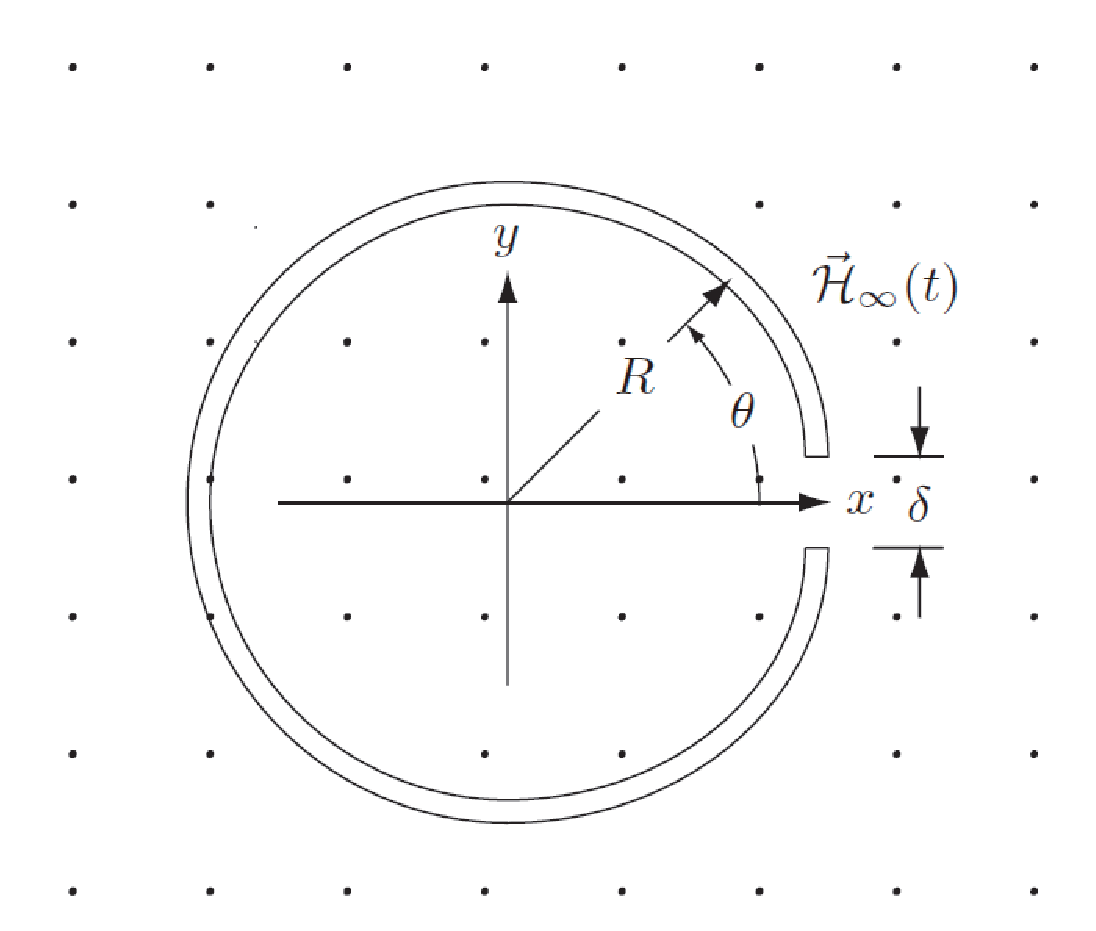
\includegraphics[scale=0.4]{chpt2/figs/fig2.9.eps}
  \caption{置于z向正弦时变磁场的在$\theta=0$处有窄缝的半径为R的理想导体长薄圆柱体的轴向视图。}
\end{figure}

\subsubsection*{问题2.6之解}
a)对一阶电场$\vec{E}_1(t)$应用积分形式的Faraday定律:
\begin{equation*}
\CMcal{V}_1(t) \equiv \int_{C} \vec{E}_1 (t) \cdot d\vec{s}=-\pi R^2 \mu_0 \frac{d\CMcal{H}_0(t)}{dt} \tag{S6.1}
\end{equation*}

线积分沿着圆柱逆时针进行(含窄缝)。上式右侧包括圆柱($\pi R^2$)所定义的整个区域。
因为圆柱是理想导体,故在材料内有$\vec{\mathcal{E}}_1(t)=0$。对线积分,仅有的非零贡献来自窄缝。以复幅值表示,有
\begin{equation*}
V_{1|0}=-j\omega \pi R^2 \mu_0 H_0 \tag{2.55}
\end{equation*}

b)应用Ohm定律,得到$J_1$(单位长度):
\begin{equation*}
J_1=\frac{V_{1|0}}{\rho_s} \tag{S6.2}
\end{equation*}

c)因为圆柱是理想导体。圆柱面上$\vec{E}_1$的切向分量必须为零。$\vec{E}_1$以直角离开或进入圆柱。
跨越圆柱的积分移动至窄缝左侧,积分区域减少,这令$|E_1|$变小。场线如图2.10所示。

d)这是c)的特例。从对称角度,可以准确计算出线积分。积分区域等于$\pi R^2/2$,即
\begin{equation*}
V_1 |_{\theta=-\pi/2}^{\theta=+\pi/2}=-\frac{1}{2}j\omega \pi R^2 \mu_0 H_0   \tag{S6.3}
\end{equation*}

上式和a)表明,在同一轴向距离点,跨过圆柱的电压与电压触头方位有关。记住这一点,这在存在时变磁场(外施磁场,如本例;系统中电流产生的)条件下测电压时非常重要。
超导体交流损耗的电测法就是一个非常好的例子。

\begin{figure}[htbp]
  \centering
 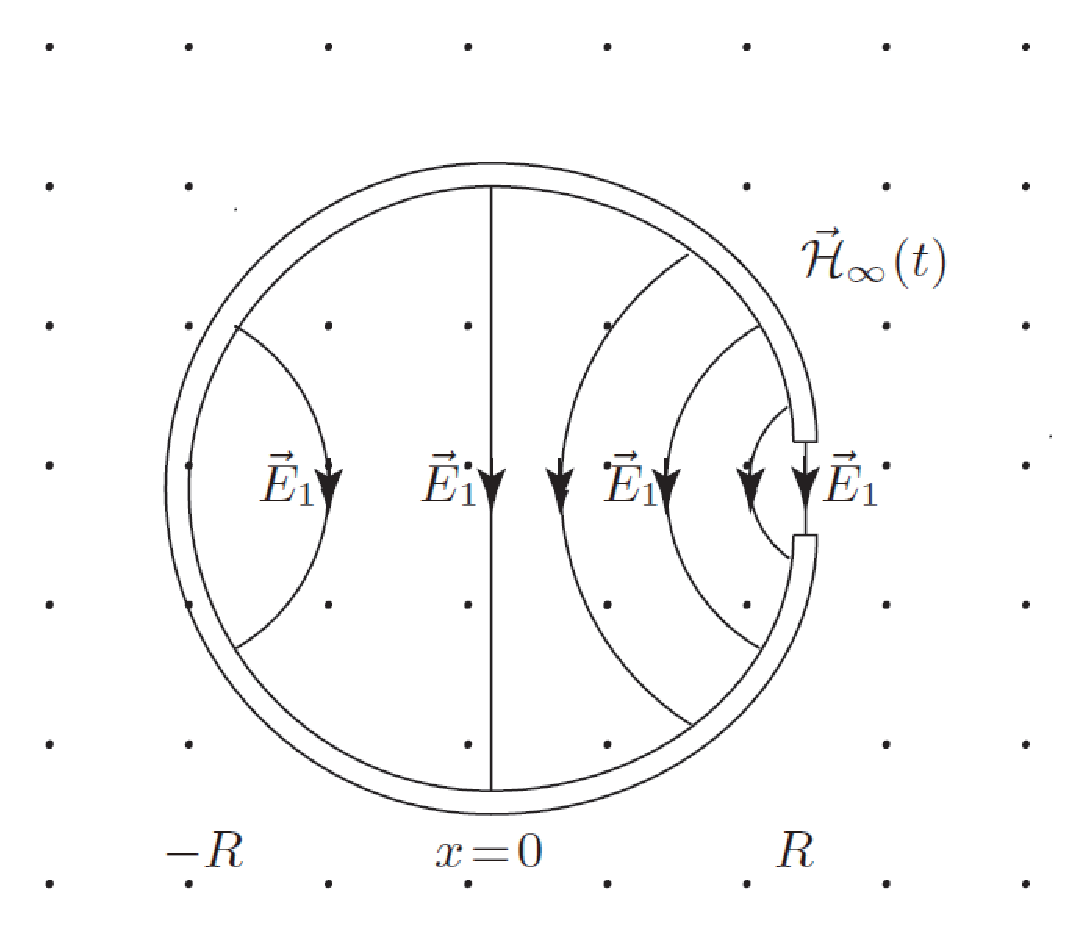
\includegraphics[scale=0.3]{chpt2/figs/fig2.10.eps}
  \caption{$\vec{E}_1$线垂直于理想导体圆柱。注意到,从$x=R$到$x=-R$,$|E_1|$是减小的。}
\end{figure}
\newpage



\subsection{问题2.7:圆柱壳的感应加热}
本问题处理金属(非超导)圆柱壳的感应加热。它是一个同时涉及时谐电磁场、能流(Poynting矢量)、能量耗散的好例子。
本体和下一题是交流损耗,特别是涡流损耗的实例,本课题将在第七章进一步讨论。
感应加热在电炉中广泛使用,用以在导体材料内获得高温。有时,也用来作为研究超导线圈热行为的研究工具。
在超导磁体技术研究中,感应加热最常以脉冲场形式在其他超导线圈中产生小的正常区域,模拟暂态扰动。

图2.11给出一个“长”金属圆柱壳,其电导率为$\rho_e$,外径为$2R$,厚度$d\ll R$,置于正弦时变磁场中。磁场的0阶分量在z向均匀。即
\begin{equation*}
\vec{\mathcal{H}}_\infty(t)=Re[H_0 e^{j\omega t}] \vec{i}_z \tag{2.54}
\end{equation*}

式中,$H_0$是复磁场幅值。

我们首先用两种方法解出相应的场量。接下来,用两种方法解出援助内的能量耗散。

\begin{figure}[htbp]
  \centering
 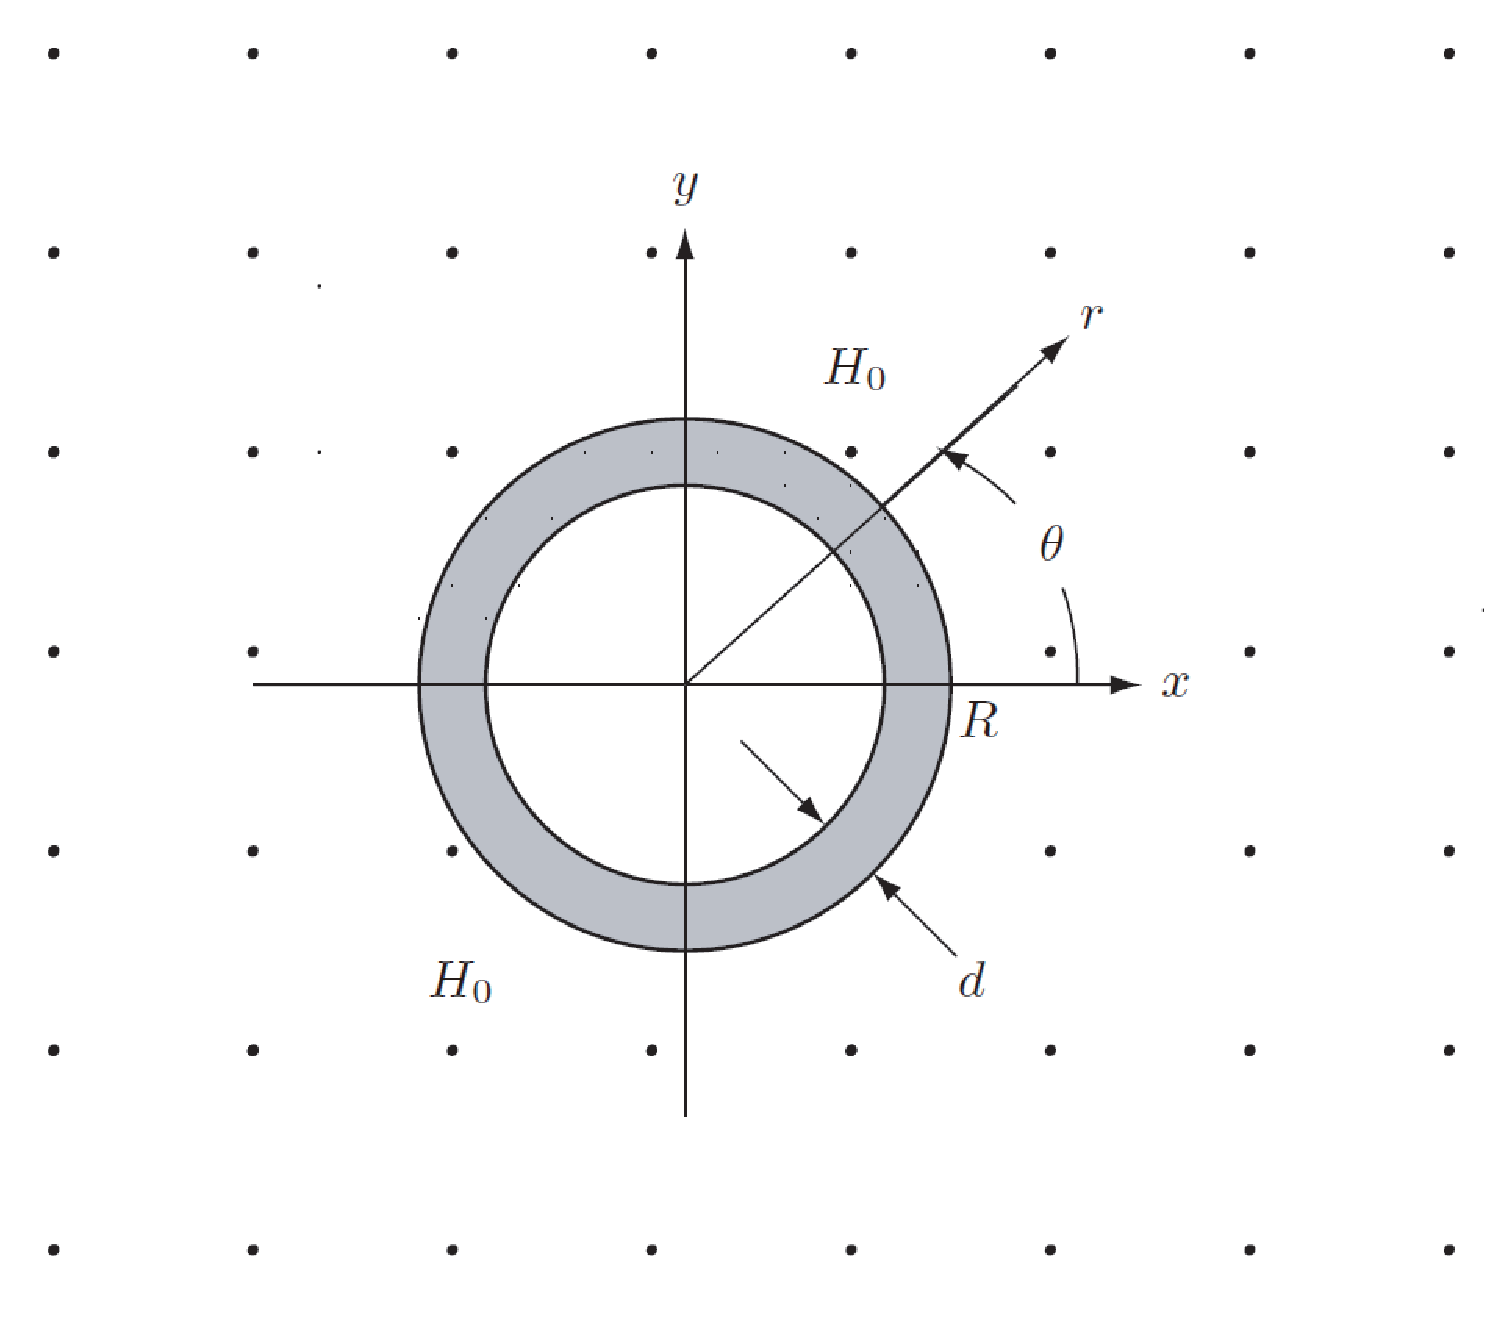
\includegraphics[scale=0.3]{chpt2/figs/fig2.11.eps}
  \caption{圆柱金属壳置于均匀正弦时变磁场之中。}
\end{figure}

\subsubsection*{第一部分:感应加热场的问题}
首先,用两种方法解出场量。

\textbf{方法一}

a)使用积分形式的Maxwell方程,忽略端部效应。证明在$r\le R$区域内给出一阶电场$\vec{E}_1$,在$r\simeq R$的壳内给出一阶电流密度$\vec{J}_1$的表达式为:
\begin{align}
\vec{E}_1=&-\frac{j\omega \mu_0 r H_0}{2} \vec{i}_\theta\\
\vec{J}_1=&-\frac{j\omega \mu_0 R H_0}{2\rho_e} \vec{i}_\theta
\end{align}

b)证明:在$r\le R-d$区域,一阶磁场$\vec{H}_1$可以表示为
\begin{equation}
\vec{H}_1=-\frac{j\omega \mu_0 R d H_0}{2\rho_e}\vec{i}_z
\end{equation} 

c)上面三式,在准静态近似条件下得出,仅在“低”频下成立,或者说仅在频率远小于“趋肤深度”频率$f_{sk}$下成立。证明:
\begin{equation}
f_{sk}=\frac{\rho_e}{\pi \mu_0 R d}
\end{equation}

\textbf{方法二}

方法一得到的$\vec{E}_1$、$\vec{J}_1$、$\vec{H}_1$均随着$\omega$增大,仅在频率小于$f_{sk}$时成立。下面,我们用一种新技术来推出在所有频率下均成立
的室温孔内场$\vec{H}_T=\vec{H}_0+\vec{H}_r$的完整表达式。式中,$\vec{H}_T$是总场,$\vec{H}_0$是原场,$\vec{H}_R$是室温孔内的系统反应场。

本方法中,首先将$\vec{H}_T=\vec{H}_0+\vec{H}_r$视为零阶场,解出作为一阶磁场响应的$\vec{H}_R$。

d)证明在$d\ll R$条件下壳内的$\vec{H}_R$、$\vec{H}_T$和$\vec{J}$为:
\begin{align}
\vec{H}_R=&-\frac{j\omega \mu_0 R d H_0}{2\rho_e+j\omega \mu_0 R d} \vec{i}_z\\
\vec{H}_T=&\frac{2\rho_e H_0}{2\rho_e+j\omega \mu_0 R d} \vec{i}_z\\
\vec{J}=&-\frac{j\omega \mu_0 R H_0}{2\rho_e+j\omega \mu_0 R d} \vec{i}_\theta
\end{align}

\subsubsection*{第一部分:感应加热场的问题之解}
根据$\theta$方向的对称性,$\vec{E}_1$和$\vec{J}_1$在$\theta$方向为常量,两个量均为$\theta$向,且仅依赖于r。这样,Faraday感应定律可在r的边线$\mathcal{C}$
上进行,围城的面积为$\mathcal{S}$:
\begin{align}
\oint_{\mathcal{C}} \vec{E}_1 \cdot d\vec{s}=-j\omega \mu_0 \int_{\mathcal{S}} \vec{H}_0 \cdot d\vec{\mathcal{A}}\nonumber\\
\int_{0}^{2\pi} r E_{1\theta} d\theta=-j\omega \mu_0 \int_{0}^{r} 2\pi r H_0 dr\nonumber\\
E_{1\theta}\int_{0}^{2\pi} r d\theta=-j\omega \mu_0 H_0\int_{0}^{r} 2\pi r dr\nonumber\tag{S7.1}
\end{align}

在$r\le R$时
\begin{equation*}
E_{1\theta} 2\pi r = -j\omega \mu_0 H_0 \pi r^2 \tag{S7.2}
\end{equation*}

上式两侧同除$2\pi r$,有
\begin{equation*}
E_{1\theta} = -\frac{j\omega \mu_0 r H_0}{2} \tag{S7.3}
\end{equation*}

于是
\begin{equation*}
\vec{E_{1}} = -\frac{j\omega \mu_0 r H_0}{2}\vec{i}_\theta \tag{2.56}
\end{equation*}

一阶电流仅在壳内($r\simeq R$)流动:
\begin{equation*}
\vec{J}_1=\frac{\vec{E_{1}}(r\simeq R)}{\rho_e} = -\frac{j\omega \mu_0 R H_0}{2\rho_e}\vec{i}_\theta \tag{2.57}
\end{equation*}

在$d\ll R$时,我们可以将电流处理为一阶表面电流$\vec{K}_1$:
\begin{equation*}
\vec{K}_1=\vec{J}_1 \cdot d= -\frac{j\omega \mu_0 R d H_0}{2\rho_e}\vec{i}_\theta \tag{S7.4}
\end{equation*}

b)对$r>R$,$\vec{H}_1=0$;我们可以将上述面电流等效为在$r=R$处$\vec{H}$的不连续:壳内壁$\vec{H}_0+\vec{H}_1$,壳外$\vec{H}_0$。于是
\begin{align}
\vec{K}_1=&\vec{i}_r \times [\vec{H}_0-(\vec{H}_0+\vec{H}_1)]=-\frac{j\omega \mu_0 R d H_0}{2\rho_e}\vec{i}_\theta\nonumber\\
=&\vec{i}_r\times-\vec{H}_1=-\frac{j\omega \mu_0 R d H_0}{2\rho_e}\vec{i}_\theta\nonumber\tag{S7.5}
\end{align}

在$d\ll R$条件下解出$\vec{H}_1(r\le R-d)$
\begin{equation*}
\vec{H}_1=-\frac{j\omega \mu_0 R d H_0}{2\rho_e}\vec{i}_z \tag{2.58}
\end{equation*}

c)前已表明,$\vec{J}_1$、$\vec{K}_1$和$\vec{H}_1$的幅值均随着频率单调增长。这意味着它不可能在所有$\omega$下成立。
事实上,那些解仅在准静态近似可以应用的低频下有效。特别的,仅在$|\vec{H}_1|\ll |\vec{H}_0|$时有效:
\begin{equation*}
|\vec{H}_1|=\frac{\omega \mu_0 R d |H_0|}{2\rho_e}\ll |\vec{H}_0|\tag{S7.6}
\end{equation*}

由上式,可以得到频率极限,即通常所谓的趋肤深度频率$f_{sk}$。在此频率下,准静态近似是有效的
\begin{equation*}
f_{sk}=\frac{\rho_e}{\pi \mu_0 R d} \tag{2.59}
\end{equation*}

注意,$f_{sk}$不仅与材料的电阻率有关,还与处于正弦时变磁场中的物体的尺寸有关。

d)在计算反应场时,设定$\vec{H}_1\equiv \vec{H}_R$。在$\vec{H}_1$的表达式中,用$\vec{H}_0+\vec{H}_R$代换$\vec{H}_0$
\begin{equation*}
\vec{H}_R=-\frac{j\omega \mu_0 R d (\vec{H}_0+\vec{H}_R)}{2\rho_e} \tag{S7.7}
\end{equation*}

解出$\vec{H}_R$,得到
\begin{equation*}
\vec{H}_R=-\frac{j\omega \mu_0 R d \vec{H}_0}{2\rho_e+j\omega \mu_0 R d}\vec{i}_z \tag{2.60}
\end{equation*}

联立方程2.60和$\vec{H}_T=\vec{H}_0+\vec{H}_R$,可以得到
\begin{align}
\vec{H}_T=\vec{H}_0+\vec{H}_R=H_0\left(1-\frac{j\omega\mu_0 R d}{2\rho_e+j\omega\mu_0 Rd}\right)\vec{i}_z\nonumber\\
=\frac{2\rho_e H_0}{2\rho_e+j\omega \mu_0 R d}\vec{i}_z\nonumber\tag{2.61}
\end{align}

$\vec{J}$和$\vec{H}_R$通过$\nabla\times \vec{H}=\vec{J}$相联系,又$\vec{K}=\vec{J}d$,于是
\begin{align}
\vec{J}=&\frac{1}{d}H_R \vec{i}_\theta \nonumber\tag{S7.8}\\
=&-\frac{j\omega \mu_0 R H_0)}{2\rho_e+j\omega \mu_0 R d}\vec{i}_\theta\nonumber\tag{2.62}
\end{align}

注意到,在低频下,$\vec{H}_R$退化为$\vec{H}_1$;高频下,$\vec{H}_R$退化为$-\vec{H}_0$而$\vec{H}_T$变为$0$。$\vec{J}$存在类似的行为。

\subsubsection*{第二部分:感应加热的能量耗散}
我们用两种方法解出圆柱内的能量耗散。

\textbf{方法一}

e)我们可以直接计算$<p>=\vec{E}\cdot \vec{J}^* /2=\rho_e |J|^2 /2$而得到圆柱壳的电阻功率损耗。式中的$\vec{J}$已在前文求出。
证明:在$d\ll R$条件下,壳内的时均总损耗(单位长度)的表达式为
\begin{equation}
<P>=2\pi R d<p>=\frac{\pi \rho_e \omega^2 \mu_0^2 R^3 d}{4\rho_e^2+\omega^2\mu_)^2 R^2 d^2} |H_0|^2
\end{equation}

\textbf{方法二}

相同的施于圆柱的复功率也可以视为从$r>R$处的源在$r=R$处进入圆柱内的Poynting能流。

f)证明:在$r=R$处,进入圆柱的一阶复Poynting矢量$\vec{S}_1$的面积分(单位长度)为:
\begin{equation}
-\oint_{\mathcal{S}}\vec{S}_1 \cdot d\mathcal{A}=\frac{1}{2}(2\pi P)E_{1\theta} H_)^*=\frac{j\pi\rho_e\omega\mu_0 R^2}{2\rho_e+j\omega\mu_0 R d}|H_0|^2
\end{equation}

提示:$E_{1\theta}=\rho_e J_\theta$,$J_\theta$已在上文求出。

g)证明:上式的等号右侧的实部与e)中给出的$<P>$是一致的。

h)画出$<P>$与$\rho_e$的关系。由于理想导体($\rho_e=0$)和理想绝缘体($\rho_e=\infty$)均不产生损耗,图像应从$<P>=0$开始,并在$\rho_e \rightarrow \infty$时趋于0。

i)从$<P>$与$\rho_e$的关系可以得到一个结论,即存在临界电阻率$\rho_{e_c}$,在该点$<P>$最大。证明
\begin{equation}
\rho_{e_c}=\frac{\omega \mu_0 R d}{2}
\end{equation}

从上式可知,对一个电阻率($\rho_e$)和样品尺寸($R,d$)组合,存在一个可以令加热最大化的最优频率。这个频率就是前面提到的趋肤深度频率$f_{sk}$。

j)计算一个半径$R=10\ \mathrm{mm}$,壁厚$d=0.5\ \mathrm{mm}$,电阻率$\rho_e=2\times 10^{-10}\ \mathrm{\Omega\cdot m} $(大致为液氦温度下铜的电阻率)的铜管的$f_{sk}$。

\subsubsection*{第二部分:感应加热的能量耗散之解}
e)正弦情况下,时均能耗(单位长度)功率可以表示为$<p>=\vec{E}\cdot \vec{J}^* /2=\rho_e |J|^2 /2$,也即
\begin{equation*}
<p>=\rho_e |J|^2 /2=\frac{\rho_e}{2}(\frac{\omega^2 \mu_0^2 R^2}{4\rho_e^2+\omega^2 \mu_0^2 R^2 d^2})|H_0|^2 \tag{S7.9}
\end{equation*}

于是,壳内总的能耗(单位长度)可以能耗功率乘以截面积得到
\begin{equation*}
<P>=2\pi R d<P>=\frac{\pi \rho_e \omega^2 \mu_0^2 R^3 d}{4\rho_e^2+\omega^2 \mu_0^2 R^2 d^2}|H_0|^2 \tag{2.63}
\end{equation*}

下面检查一下上式在$\rho_e$两个极限下的情况:
\begin{align}
&\rho_e \ll \omega \mu_0 R d\mbox{(良导体)时:}<P>\simeq \frac{\pi \rho_e R}{d}|H_0|^2\propto \rho_e\nonumber\tag{S7.10a}\\
&\rho_e \gg \omega \mu_0 R d\mbox{(不良导体)时:}<P>\simeq \frac{\pi \omega^2 \mu_0^2 R^3 d}{4\rho_e}|H_0|^2\propto \frac{1}{\rho_e}\nonumber\tag{S7.10b}
\end{align}

正如我们所期望的,在上面两种极限情况下,都有$<P>\rightarrow 0$。

f)复Poynting矢量$\vec{S}$的一阶展开为:
\begin{equation*}
\vec{S}_1=\frac{1}{2}(\vec{E}_0 \times \vec{H}_0^*+\vec{E}_0 \times \vec{H}_1^*+\vec{E}_1 \times \vec{H}_0^*) \tag{S7.11}
\end{equation*}

计算一阶Poynting矢量时,$E$和$H$场的下表均不大于1。在本例下,我们有$\vec{E}_0=0$,于是上式化简为:
\begin{equation*}
\vec{S}_1=\frac{1}{2}(\vec{E}_1 \times \vec{H}_0^*) \tag{S7.12}
\end{equation*}

对于$\vec{E}_1$我们有:
\begin{equation*}
\vec{E}_1=\rho_e \vec{J}=-\frac{j\rho_e \omega \mu_0 R H_0)}{2\rho_e+j\omega \mu_0 R d}\vec{i}_\theta \tag{S7.13}
\end{equation*}

于是,
\begin{equation*}
-\oint_{\mathcal{S}}\vec{S}_1 \cdot d\mathcal{A}=\frac{1}{2}(2\pi R)E_{1\theta} H_0^*=\frac{j\pi\rho_e \omega \mu_0 R^2}{2\rho_e+j\omega \mu_0 R d} |H_0|^2 \tag{2.64}
\end{equation*}

g)根据复数的基本运算法则,取f)最后结果的实部,易得。可以看到,这和方法一得到的结果是一致的。
\begin{equation*}
<P>=\frac{\pi \rho_e \omega^2 \mu_0^2 R^3 d}{4\rho_e^2+\omega^2 \mu_0^2 R^2 d^2}|H_0|^2 \tag{S7.14}
\end{equation*}

h)如图2.12所示。

i)将$<P>$对$\rho_e$求导,并令之为零,有:
\begin{equation*}
\frac{d<P>}{d\rho_e} |_{\rho_{e_c}}=[**]=0 \tag{S7.15}
\end{equation*}

解出上式,有
\begin{equation*}
\rho_{e_c}=\frac{\omega \mu_0 R d}{2} \tag{2.65}
\end{equation*}

上式在均匀正弦时变磁场施加于导体样品的感应加热应用中非常重要。样品被样品中感应的涡流加热。在趋肤深度频率$f_{sk}$下,感应加热最大。

j)将数值$R=1\ \mathrm{cm}, d=0.5\ \mathrm{mm},\rho_e=2\times 10^{-10}\ \mathrm{\Omega m}$(4K时铜的电阻率)代入公式,有
\begin{equation*}
f_{sk}=\frac{\rho_{e_c}}{\pi\mu_0 R d}\simeq 10Hz \tag{2.59}
\end{equation*}

\begin{figure}[htbp]
  \centering
 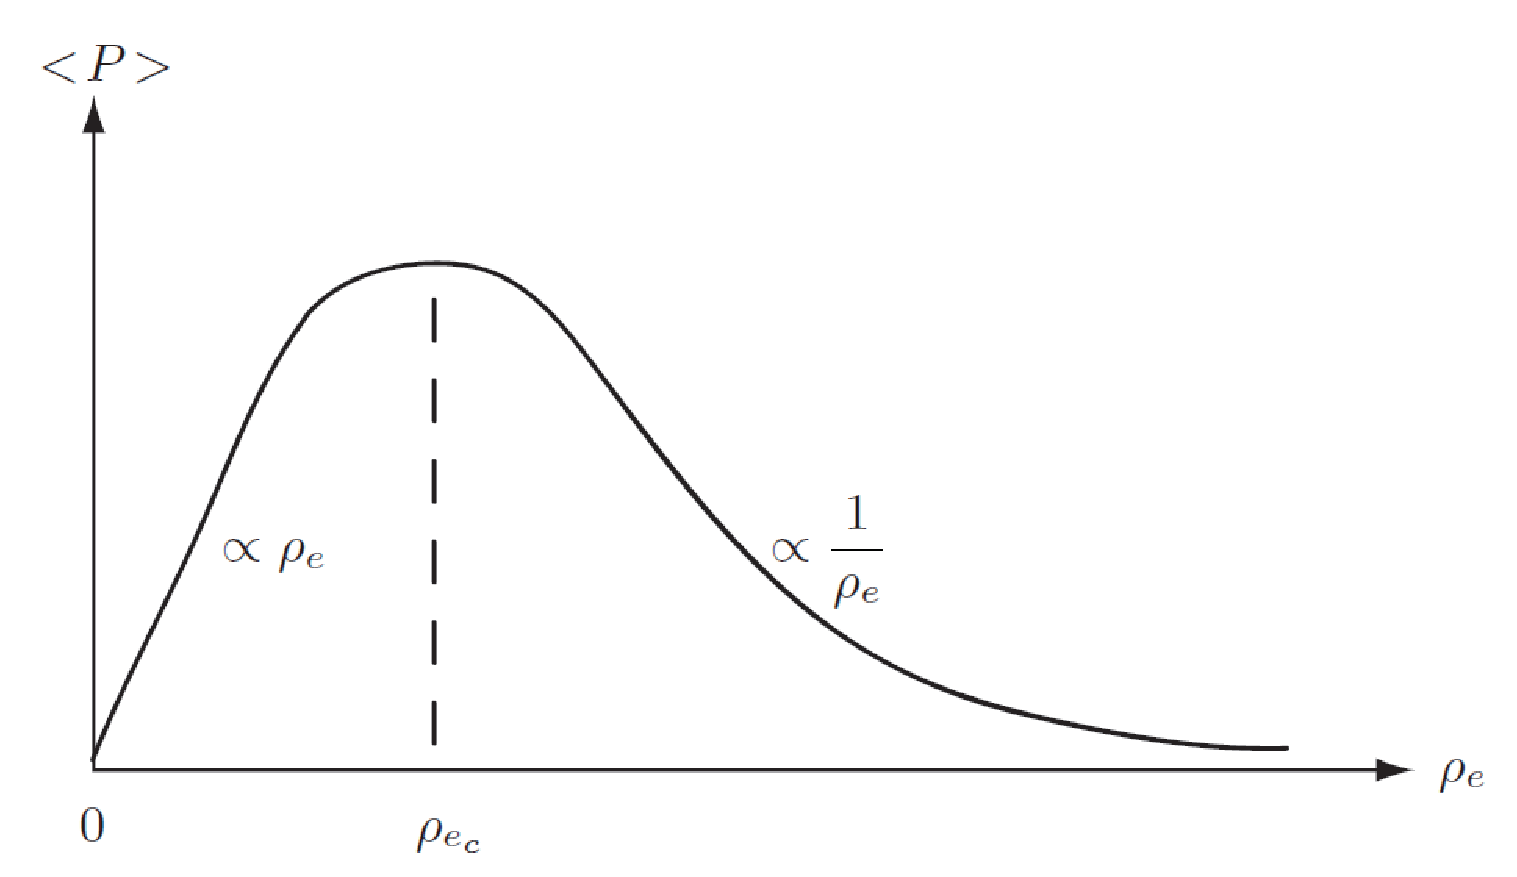
\includegraphics[scale=0.3]{chpt2/figs/fig2.12.eps}
  \caption{感应加热圆柱壳的功率耗散和电阻率的关系。}
\end{figure}
\newpage



\subsection{问题2.8:金属窄带中的涡流损耗}
本题推导置于时变磁场中的金属窄带的涡流损耗。这可以用于计算铜基超导带中涡流损耗的计算。(感应电流有用时叫感应加热,有害时就叫涡流损耗。)

图2.13给出了电导率为$\rho_e$、$y$向宽为$b$、厚度($z$向)为$a$的长($x$向)金属窄带。窄带置于时变外磁场中。外场满足$dB_0/dt=\dot{B_0}$,即零阶、均匀、$z$向。

a)证明一阶电场$\vec{E}_1$为
\begin{equation}
E_{1x}=y\dot{B_0}
\end{equation}

b)证明空间平均能耗密度$\tilde{p}$(单位体积)为:
\begin{equation}
\tilde{p}=\frac{(b\dot{B_0})^2}{12\rho_e}
\end{equation}

c)外场以角频率$\omega$正弦变化,即$B(t)=B_0 \sin\omega t$时,证明:时均能耗密度为:
\begin{equation}
<\tilde{p}>=\frac{(b\omega\dot{B_0})^2}{24\rho_e}
\end{equation}

\begin{figure}[htbp]
  \centering
 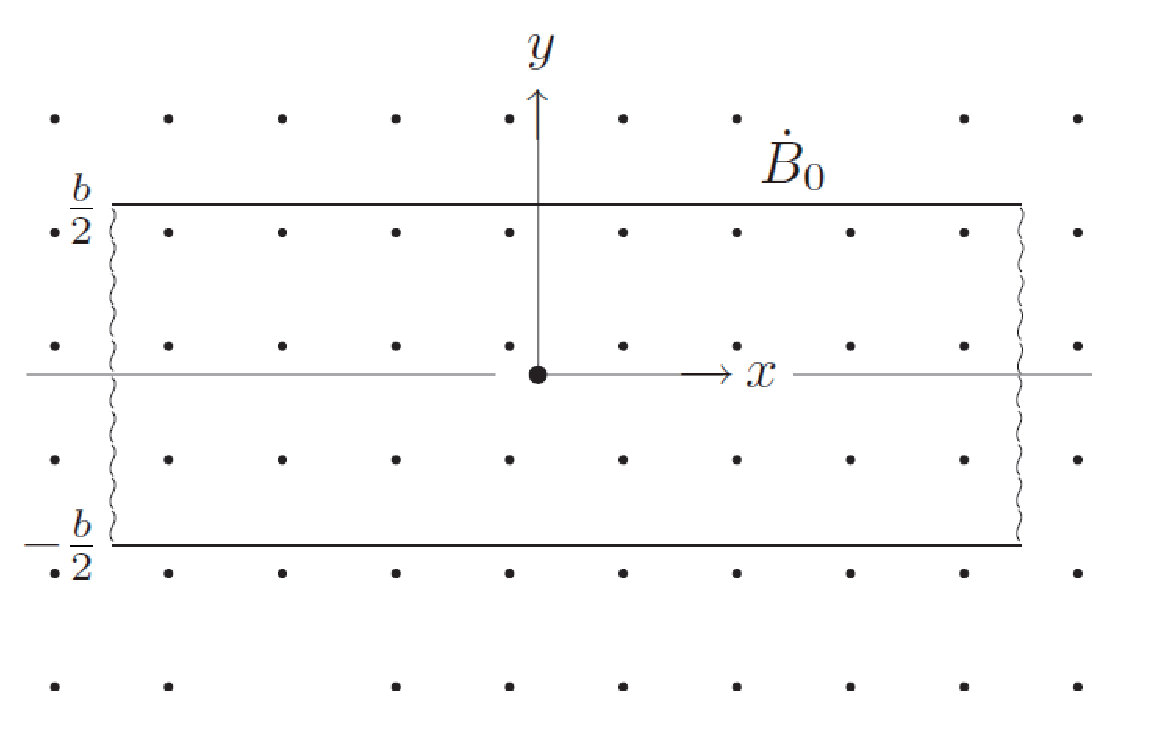
\includegraphics[scale=0.4]{chpt2/figs/fig2.13.eps}
  \caption{宽度为b的金属窄带置于时变磁场中。}
\end{figure}

\subsubsection{问题2.8之解}
a)由于$\vec{B}_0$时均匀分布的且系统不依赖于$x$,所以$\vec{E}_1$只能指向$x$方向并且仅依赖于$y$。于是$\nabla\times \vec{E}_1=\partial \vec{B}_0/\partial t$可以化简为
\begin{equation*}
-\frac{dE_{1x}}{dy}=-\frac{B_0}{dt}=-\dot{B}_0 \tag{S8.1}
\end{equation*}

根据对称性,$E_{1x}(y=0)=0$,于是,我们有
\begin{equation*}
E_{1x}=y\dot{B_0}  \tag{2.66}
\end{equation*}

b)窄带中的局部能量损耗密度$p(y)$由$\vec{E}_1\cdot\vec{J}_1$给出。总的损耗(单位长度)为
\begin{equation*}
P=a\int_{-b/2}^{b/2}p(y)dy=\frac{2a(\dot{B}_0)^2}{\rho_e}\int_{0}^{b/2}y^2dy=\frac{ab(b\dot{B_0})^2}{12\rho_e}  \tag{S8.2}
\end{equation*}

上式仅在$\vec{J}_1$感应出来的一阶感应磁场相比$\vec{B}_0$很小时才有效。

空间平均能耗密度$\tilde{p}$(单位体积)可以由$P$除以截面得到:
\begin{equation*}
\tilde{p}=\frac{P}{ab}\frac{(b\dot{B_0})^2}{12\rho_e}  \tag{2.67}
\end{equation*}

c)在外场正弦变化时,时均能耗密度为:
\begin{equation*}
<\tilde{p}>=\frac{1}{2}E_{1x} J_{1x}^*  \tag{S8.3}
\end{equation*}

由于$E_{1x}=j\omega y B_0$,$J_{1x}=E_{1x}/\rho_e$,于是可以得到
\begin{equation*}
<\tilde{p}>=\frac{2a(\omega B_0)^2}{2\rho_e (ab)}\int_{0}^{b/2} y^2 dy=\frac{(b\omega\dot{B_0})^2}{24\rho_e}  \tag{2.68}
\end{equation*}

我们注意到,$\tilde{p}$和$<\tilde{p}>$分别正比于$(b\dot{B_0})^2$和$(b\omega \dot{B_0})^2$。也就是说,两者对感应磁场和导体宽度均为平方依赖关系。
\newpage



\subsection{讨论2.4:分层以减少涡流损耗}
假设将薄板劈为两条,每一条宽度为$b/2$,由上面的分析可以知道,损耗将变为原来的$1/4$。因此,可以通过将窄带细分的方法降低涡流损耗。这种切分技术在电力变压器中广泛使用。类似的,我们将在第5章和第7章中看到,超导体也能从切分中获益。
\newpage


\subsection{问题9:Rogowski线圈}
Rogowski线圈是时变电流的安培计。它是一种环形拾磁线圈,其积分输出电压正比于被线圈包围的截面内通过的总电流。图2.14a给出了一个Rogowski线圈,待测电流$I(t)$置于其中央。如图所示,Rogowski线圈包括$N$个串联的小圆环(一匝)。每一个半径为$c$的圆环的中心位于电流中心的径向$R$处。
图2.14b定义了一匝的$xy$坐标。

a) 证明在$c\ll R$条件下,$N$匝的Rogowski线圈的总磁链$\Phi(t)=N\Phi_1(t)$为:
\begin{equation}
\Phi(t)\simeq\frac{\mu_0 N c^2}{2R}I(t)
\end{equation}

式中,$\Phi_1(t)$是与一匝交链的总磁通。

b) 证明$\Phi(t)$的准确表达式为:
\begin{equation}
\Phi(t)=\mu_0 N (R-\sqrt{R^2-c^2})I(t)
\end{equation}

将$N$匝中的一个放在$xy$坐标系的中心来计算$\Phi(t)$。

c) 证明在极限$(c/R)^4\ll 1$下,b)退化为a)。

d)证明b)中的公式在Rogowski线圈的轴线偏离电流的中心时也有效。

e)计算一个$N = 3600; c = 3\ \mathrm{mm}; R = 0.5\ \mathrm{m}$的Rogowski线圈在$\Delta I(t)=1\ \mathrm{MA}$时两端产生的伏秒。

\begin{figure}[htbp]
  \centering
 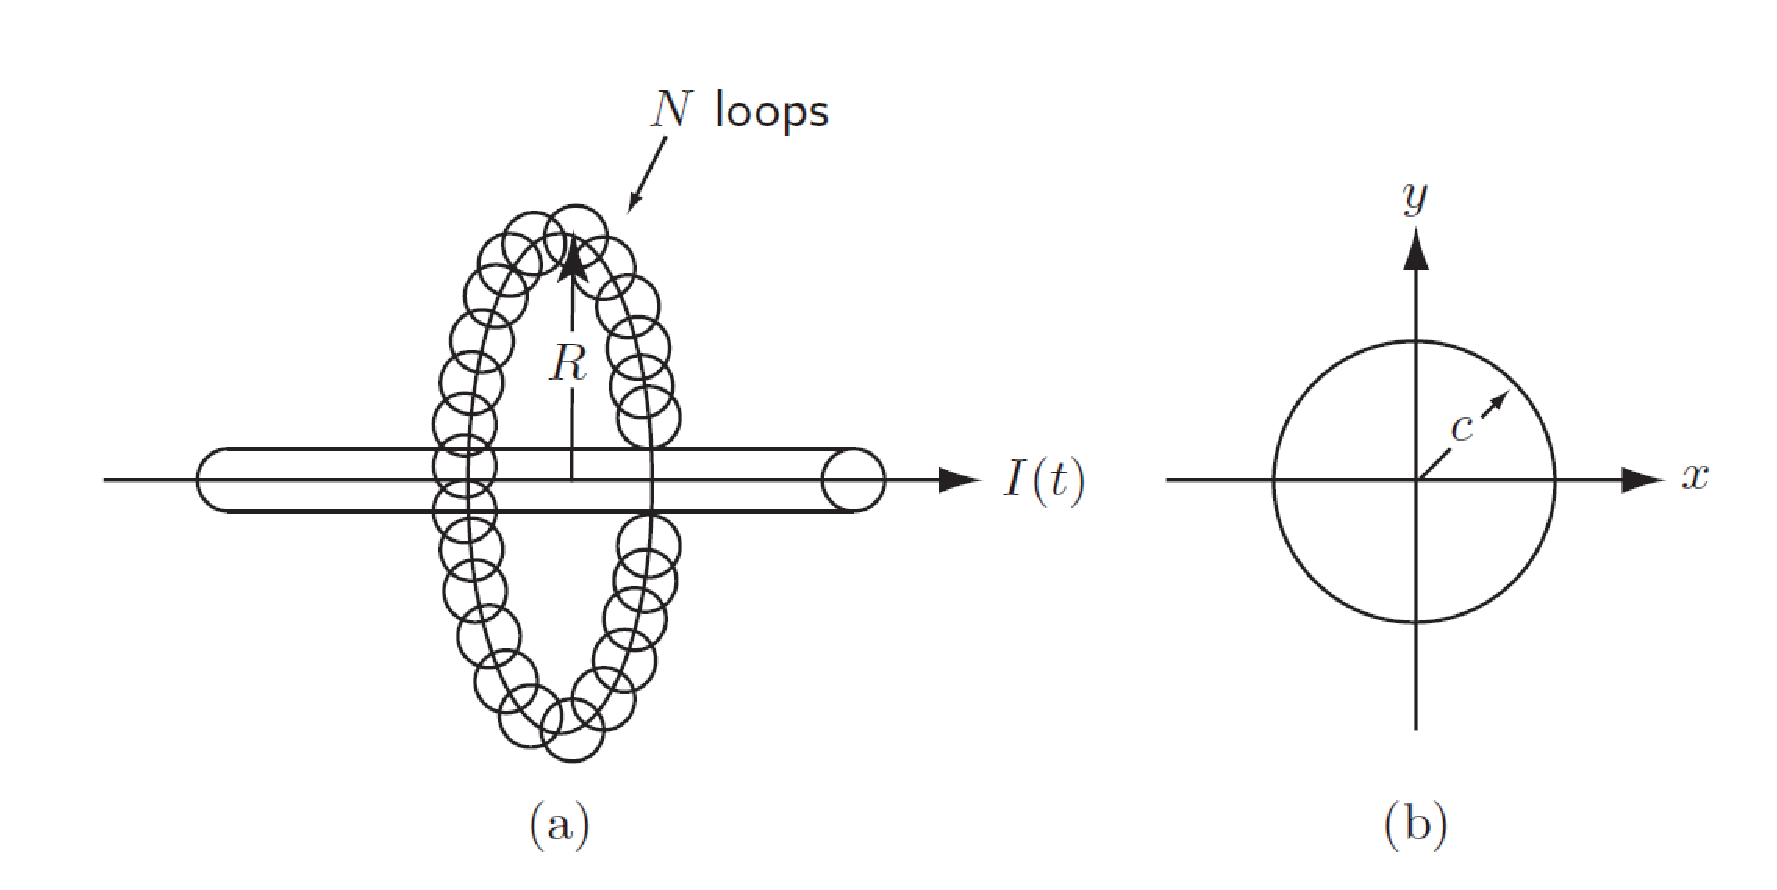
\includegraphics[scale=0.4]{chpt2/figs/fig2.14.eps}
  \caption{(a)$N$匝Rogowski线圈,每匝直径为$2c$,环绕在待测的时变电流$I(t)$外围。(b)一匝(半径为$r$)的截面视图。圆环距离电流中心的距离为$R$。}
\end{figure}

\subsubsection{问题13之解}
a)电流$I(t)$产生的磁场相对于电流方向是方位角向的。距电流中心距离$R$处的$H_\phi(t)$表示为:
\begin{equation*}
H_\phi (t)=\frac{I(t)}{2\pi R} \tag{S9.1}
\end{equation*}

对于$c\ll R$,上式给出的$H_\phi(t)$在每一匝的横截面$\pi c^2$上几乎都是成立的。由于Rogowski线圈有$N$个这样的回路,我们有:
\begin{equation*}
\Phi(t)\simeq \frac{\mu_0 N c^2}{2R}I(t)  \tag{2.69}
\end{equation*}

Rogowski线圈输出电压$V(t)$于是可以写为:
\begin{equation*}
V(t)=\frac{d\Phi(t0}{dt}=\frac{\mu_0 N c^2}{2R}\frac{dI(t)}{dt}  \tag{S9.2}
\end{equation*}

b)因为$H_\phi (t)$在每一个环上并非常数,每一匝包围的总磁通$\Phi_1(t)$应由沿回路围成的区域的积分得到。
注意到$x^2+y^2=c^2$,定回路中心坐标为$(0,0)$,$\Phi_1(t)$表示为:
\begin{align}
\Phi (t)=&\frac{\mu_0 I(t)}{2\pi}\int_{-c}^{c}\int_{-\sqrt{c^2-y^2}}^{\sqrt{c^2-y^2}}\frac{1}{R+y}dxdy\nonumber\\
=&\frac{\mu_0 I(t)}{\pi}\int_{-c}^{c}\frac{\sqrt{c^2-y^2}}{R+y}dy\nonumber\tag{S9.3}
\end{align}

上式可以使用新变量$\xi\equiv R+y$得到闭式解(注意:$d\xi=dy$)。于是,有:
\begin{align}
\Phi_1 (t)=&\frac{\mu_0 I(t)}{\pi} \int_{R-c}^{R+c}\frac{\sqrt{c^2-R^2+2R\xi-\xi^2}}{\xi}d\xi\nonumber\\
=&\mu_0(R-\sqrt{R^2-c^2})I(t)\nonumber\tag{S9.4}
\end{align}

$N$匝的Rogowski线圈交链的总磁通$\Phi(t)=N\Phi_1(t)$:
\begin{equation*}
\Phi (t)=\mu_0 N(R-\sqrt{R^2-c^2})I(t) \tag{2.70}
\end{equation*}

c)上式可以写为:
\begin{equation*}
\Phi (t)=\mu_0 NI(t)(R-R\sqrt{1-\frac{c^2}{R^2}}) \tag{S9.5}
\end{equation*}

由于对$x\ll 1$,$\sqrt{1-x}\simeq 1-(1/2)x+(1/8)x^2-...$,截取到二阶,所以
\begin{align}
\Phi(t)\simeq\mu_0 N\left[R-R\left(1-\frac{1}{2}\frac{c^2}{R^2}+\cdots\right)\right]\nonumber\tag{S9.6}\\
\Phi (t)\simeq \frac{\mu_0 Nc^2}{2R} I(t)\nonumber\tag{2.69}
\end{align}

\begin{figure}[htbp]
	\centering
	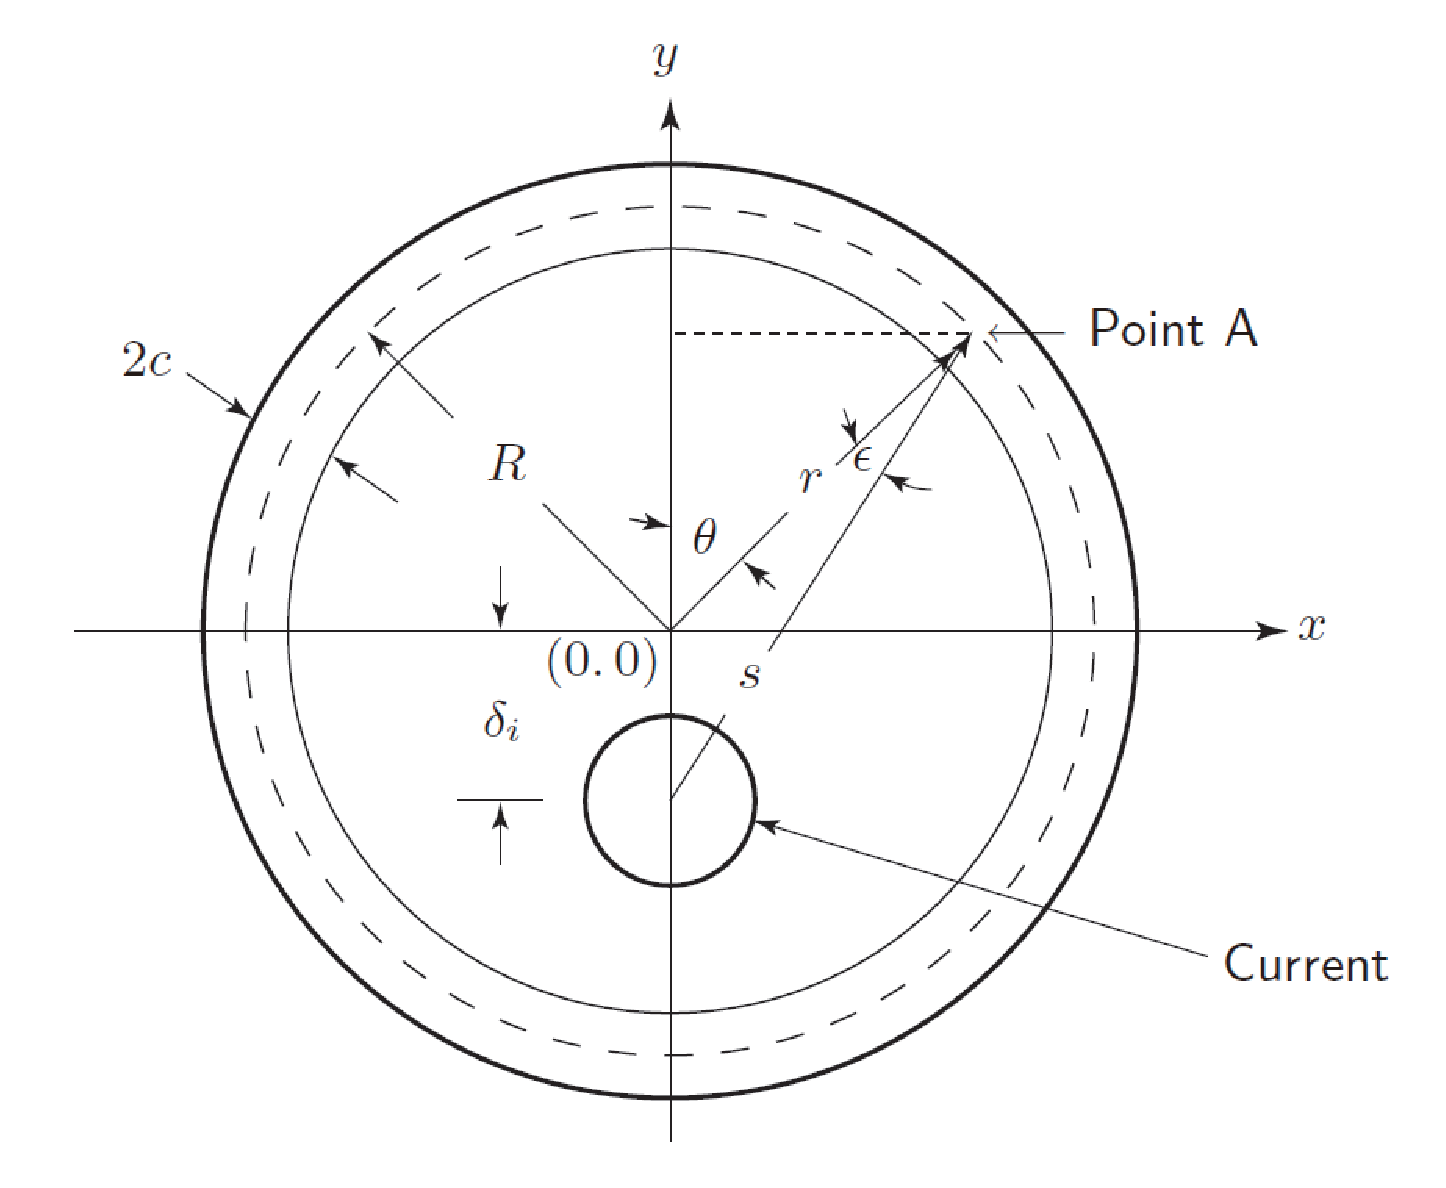
\includegraphics[scale=0.3]{chpt2/figs/fig2.15.eps}
	\caption{$(x,y)$面上的横截面视图。}
\end{figure}

d)图2.15给出正交于电流/Rogowski线圈组方向的横截面$(x,y)$,其中Rogowski中心位于$(0,0)$,电流中心在Rogowski线圈中心向下偏离$\delta_i$。关键参数如图中定义:$r$为Rogowski中心$(0,0)$到一匝线圈上的点$A$的径向距离;$\theta$是$y$轴和$r$之间的夹角;$s$是电流中心到点$A$的距离;$\epsilon$是$r$与$s$之间形成的角。$s^2$写为:
\begin{equation*}
s^2=(r\cos\theta+\delta_i)^2+r^2\sin^2\theta=r^2+\delta_i^2+2r\delta_i\cos\theta \tag{S9.7}
\end{equation*}

将$r$延长$\delta_i \cos\theta$形成一个直角,我们有:
\begin{equation*}
\cos\epsilon=\frac{r+\delta_i \cos\theta}{s} \tag{S9.8}
\end{equation*}

点$A$处的磁场由$H_A(t)=I(t)/2\pi s$给出;它在Rogowski线圈回路上点$A$处的法向分量为:
\begin{equation*}
H_{A\bot}=\frac{I(t)}{2\pi s}\cos\epsilon=\frac{I(t)}{2\pi s}(\frac{r+\delta_i \cos\theta}{s}) \tag{S9.9}
\end{equation*}

将上式与$s^2$的表达式联立,得到:
\begin{equation*}
H_{A\bot}=\frac{I(t)}{2\pi}\left(\frac{r+\delta_i \cos\theta}{r^2+\delta_i^2+2r\delta_i\cos\theta}\right) \tag{S9.10}
\end{equation*}

为了计算$\Phi(t)$,$S9.10$乘上$(N/2\pi)2\sqrt{c^2−(r−R)^2}$必须积分两次:第一次对$\theta$从$0$至$2\pi$积分,视径向距离$r$为常数,计及$N$匝;第二次对$R$从$R-c$到$R+c$积分。注意到$2\sqrt{c^2−(r−R)^2}$是每一匝直径为$c$的线圈在$r$处总的弦距离($z$向),它位于距离回路中心的$r-R$处。
\begin{align}
\Phi(t)&=\frac{N I(t)}{2\pi^2}\int_{R-c}^{R+c}\int_{0}^{1\pi}\left[ \frac{(r+\delta_i \cos\theta)\sqrt{c^2-(r-R)^2}}{r^2+\delta_i^2+2r\delta_i \cos\theta}\right]d\theta dr\nonumber\tag{S9.11a}\\
&=\frac{N I(t)}{\pi}\int_{R-c}^{R+c} \left[ 0+\frac{\sqrt{c^2-(r-R)^2}}{r}\right]dr\nonumber\tag{S9.11b}
\end{align}

注意到积分中完全没有$\delta_i$。下面,$S9.11b$沿着一匝的径向从$r=R-c$到$r=R+c$积分,有:
\begin{equation*}
\Phi(t)=\frac{N I(t)}{\pi}\left[ \pi(R-\sqrt{R^2-c^2})\right] \tag{S9.11c}
\end{equation*}

可见,Rogowski线圈可以精确的测量电流$I(t)$,不管它与其套入的电流是否同心。

e) 对于$N = 3600, c = 3\ \mathrm{mm}; R = 0.5\ \mathrm{m}; \Delta I = 1\ \mathrm{MA}$,公式2.69可以应用,因为$(c/R)^4 = 1.3×10^{−9}\ll 1$。这样,由$S9.2$得:
$$\int V(t)dt=\frac{\mu_0 N c^2 \Delta I}{2R}\simeq 41\ \mathrm{mVs}$$

在一个噪音环境中,比如典型的试验聚变机器中,测到$40\ \mathrm{mVs}$级别的信号水平并不简单,但也不是完全得不到。

\begin{quotation}
\kaishu 正如我们所知,有已知的已知,他们是我们知道我们知道的;我们也知道有些是已知的未知。这就是说我们知道有些事情我们是不知道的。但是还有未知的未知——这些事我们不知道我们不知道。——Donald Rumsfeld,2002
\end{quotation}
\newpage
\chapter{磁体、磁场和力}
\section{引言}
本章我们研究与磁体、磁场和力相关的关键主题。
涉及到的磁体包括:1)螺管磁体。单螺管磁体及多螺管磁体;
2)Helmhotz线圈和高均匀场磁体;
3)理想二极磁体;4)理想四极磁体;
5)跑道线圈;6)理想螺绕环磁体。
将会论及的还有用于产生高场的两种重要螺管磁体---Bitter磁体和混合磁体。
其他诸如负载线、最小体积磁体、叠加技术等问题将在专题中研究。

现今的磁场与力通常都交由程序计算。给定磁体的配置,程序就能得到任意位置的精确数值解。
程序也能计算组成磁体的各线圈的自感与及其之间的互感以及施于其上的Lorentz力[3.1]。
本章推导的解析解虽仅给出特定位置(如中心)的场值,但展现了磁场、力和磁体参数间的明确关系。

在简论部分,我们首先研究在无磁性材料存在时用于计算由电流产生的磁场的Biot-Savart定律。
接下来处理一些扩展性问题:1)磁场分析;2)``环形''和``薄壁''螺管的轴向力;
3)螺管内的应力应变;4)自感和互感。

\section{Biot-Savart定律}
位于$O$点的电流微元$Id\vec{s}$在距离其$r$远处的$P$点产生的磁场微元$d\vec{H}$为:
\begin{equation}\label{eqn:bs law}
  d\vec{H}=\frac{(Id\vec{s}\times \vec{r})}{4\pi r^3}
\end{equation}

式3.1称为Biot-Savart定律(又称Laplace第一定律)。
它表明,任意位置的$d\vec{H}$的幅值反比于该位置到电流元的距离平方:$|d\vec{H}|\propto 1/r^2$。
对于给定的半径,$|d\vec{H}|$随$\sin\theta$变化,其中$\theta$是矢量$\vec{s}$和$\vec{r}$的夹角。
应用式3.1,我们推导位于$z=0$处的载流为$I$的闭合线圈在轴向$(z)$上的磁场的表达式,如图3.1。
回路的对称轴定义为$z$轴;$\theta$从$z=0$平面算起,如图3.1所示;$\varphi$(图中未给出)是周向角。
\begin{figure}[htbp]
  \centering
 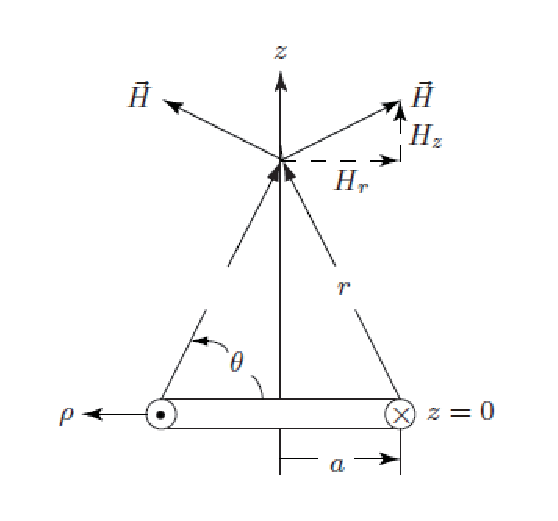
\includegraphics[scale=0.7]{chpt3/figs/fig3.1.eps}
  \caption{半径为a的闭合回路通过电流$I$。}
\end{figure}
如图3.1知,$\vec{H}$的$r$分量$H_r$在$z$轴上的任何位置都是抵消的,仅剩下$z$分量:
$dH_z=|d\vec{H}|\cos\theta$。在这个特定情况下,式3.1中的$(Id\vec{s}\times \vec{r})$可简化为
$(Id\vec{s}\times \vec{r})_z=Iar\cos\theta d\varphi$,于是
\begin{equation}\label{eqn:bs law z1}
  H_z=\int_{0}^{2\pi}\frac{Iar\cos\theta}{4\pi r^3}d\varphi=\frac{Ia\cos\theta}{2r^2}
\end{equation}
式中,$\cos\theta=a/r$,$r^2=a^2+z^2$,于是可写出$H_z(z,\rho)$在$z$轴上($\rho=0$)的场$H_z(z,0)$,
该场还可以用中心场$H_z(0,0)$表示。形式为:
\begin{subequations}\label{eqn:bs law z2}
	\begin{align}
H_z(z,0)&=\frac{a^2I}{2r^3}=\frac{a^2I}{2(a^2+z^2)^{3/2}} \\
H_z(z,0)&=\frac{H_z(0,0)}{(1+(z/a)^2)^{3/2}} 
\end{align}
\end{subequations}

式3.3a可用于推导与$\varphi$无关、任意电流分布、任意绕组截面的轴向场的表达式。
问题3.1和讨论3.1是两个很好的实例。
在试3.3b中,我们看到在$z\gg a$或远离中心时,``环''线圈的轴向场按$1/(z/a)^3$衰减---
这将在问题3.11中深入探究。

\section{Lorentz力和磁压}
在有磁感应强度$\vec{B}$存在时,以速度$\vec{v}$运动的电荷$q$会受到力$\vec{F}_L$,此力称为Lorentz力:
$\vec{F}_L=q\vec{v}\times \vec{B}$。
对于一个处于磁场$\vec{B}$中的电流密度为$\vec{J}$的导体,Lorentz力密度为:
\begin{equation}\label{eqn:lorentz force}
  \vec{f}_L=\vec{J}\times \vec{B}
\end{equation}

式3.4是磁体中磁场力和应力的基础表达式。
如第1章提到的,不管是以超导运行于1.8-80 K,还是以电阻态运行在室温,
产生相同磁场的磁体所应对的应力水平基本是一样的。
磁体的极限磁场受到结构部件(包括其载流导体)的强度的限制。
这样看,一个50 T的超导磁体---如果可能的话---和一个50 T电阻磁体都必须承受巨大的Lorentz应力。
下文将会指明,一个50 T磁体对应的磁压为$\sim 1$ GPa(10,000 atm)。

考虑一个无限长的``薄壁''(厚度$\delta$)螺管,平均半径为$2a$,通以均匀分布的电流(为了计算简便,
可等效为面电流密度$K_\theta [\mathrm{A/m}]$)。$(0,0)$处的磁感应强度$B$的$z$分量$B_z$可由式3.3a对$z$积分得到:
\begin{equation}\label{eqn:inf solenoid}
  B_z=\frac{\mu_0 a^2 K_\theta}{2}\int_{-\infty}^{\infty}\frac{dz}{(a^2+z^2)^{3/2}}=\mu_0 K_\theta\equiv B_0
\end{equation}

由于电流环的分布是从$z=-\infty$到$z=\infty$的,故积分包括整个$z$轴。
应用Ampere定律,可知对于该无限长螺管,在螺管外($r>a$),$\vec{B}$为零;
在螺管室温孔内,为$B_0$,且在$z$和$r$两个方向都均匀分布。
(从电流分布的对称性看,磁场也与$\theta$无关。同时应注意式3.3a仅在上述情况下成立。)
也就是说,无限长螺管的室温孔内的磁场是完全均匀的,且仅有$z$分量。
下面将更详细的讨论轴向磁场。

仅位于绕组内部的$B_z$就是$B_0$,位于外部的是$0$,而在管壁厚度$\delta$方向正比于$r$线性衰减。
所以,绕组中电流处于平均磁感应强度为$B_0/2$的$\~{B}_z$的磁场中。
因而,施于线圈上的$r$方向的平均Lorentz力密度为:
\begin{equation}\label{eqn:inf solenoid fl}
  f_{L_r}\vec{i}_r=\frac{K_\theta}{\delta}\~{B}_z \vec{i}_r=\frac{K_\theta B_0}{2\delta}\vec{i}_r
\end{equation}

\begin{figure}[htbp]
  \centering
 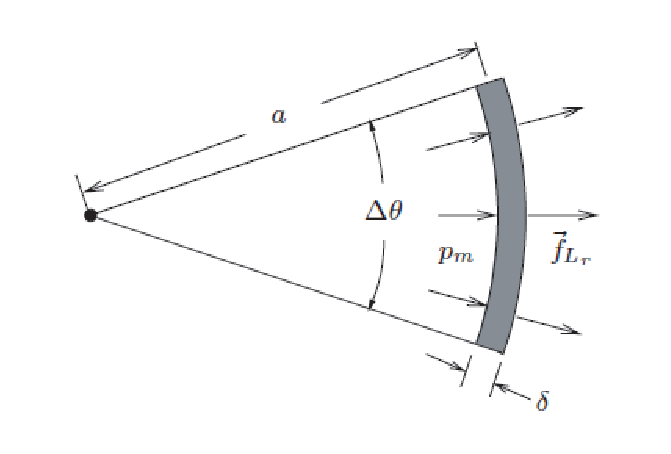
\includegraphics[scale=0.6]{chpt3/figs/fig3.2.eps}
  \caption{平均直径为$2a$的``薄壁''螺管(壁厚$\delta$)的微元的轴向视角。微元在$z$向的高度元为$\Delta z$(垂直纸面向外)。}
\end{figure}

如图3.2定义的作用于绕组体积元上的$r$向的Lorentz力$F_{L_r}\vec{i}_r$等价于作用于绕组表面元上的磁压$p_m\vec{i}_r$(定义同样如图3.2)。于是:
\begin{equation}\label{eqn:inf solenoid fl2}
  F_{L_r}\vec{i}_i =f_{L_r}[(a\Delta \theta)\delta \Delta z]\vec{i}_r=p_m[(a\Delta \theta)\Delta z]\vec{i}_r
\end{equation}

联立式3.5-3.7,解出$p_m$:
\begin{equation}\label{eqn:mag press}
  p_m=\frac{B_0^2}{2\mu_0}
\end{equation}

也即,磁压等于磁能密度。如果磁感应强度$B_0=1\ \mathrm{T}$,
根据式3.8可算得磁压为$3.98\times 10^5 \ \mathrm{Pa}$或$\sim 4\ \mathrm{atm}$。
若$B_0=50 \ \mathrm{T}$,磁压将达到$\sim 1\ \mathrm{GPa}$。

\section{螺管线圈的磁场分析}
本节,我们将推导出对分析高磁场空间均匀性的MRI和NMR磁体有用的闭式磁场
以及简单线圈(``长"和``薄壁")的磁场表达式。
在螺管线圈设计的开始阶段,可以通过这些表达式``感受''场的均匀性。

图3.3给出的是一个内径、外径和长度分别为$2a_1, 2a_2, 2b$的螺管线圈的剖面图。从磁力线可以看出,线圈产生的磁场在室温孔内主要是沿轴向的;除了线圈的对称轴上和轴中平面上,磁力线都是沿径向室温孔外发散的。
两个无量纲常数常用于螺管线圈磁场的分析:$\alpha\equiv 2a_2/2a_1=a_2/a_1$和$\beta\equiv 2b/2a_1=b/a_1$。
\begin{figure}[htbp]
	\centering
	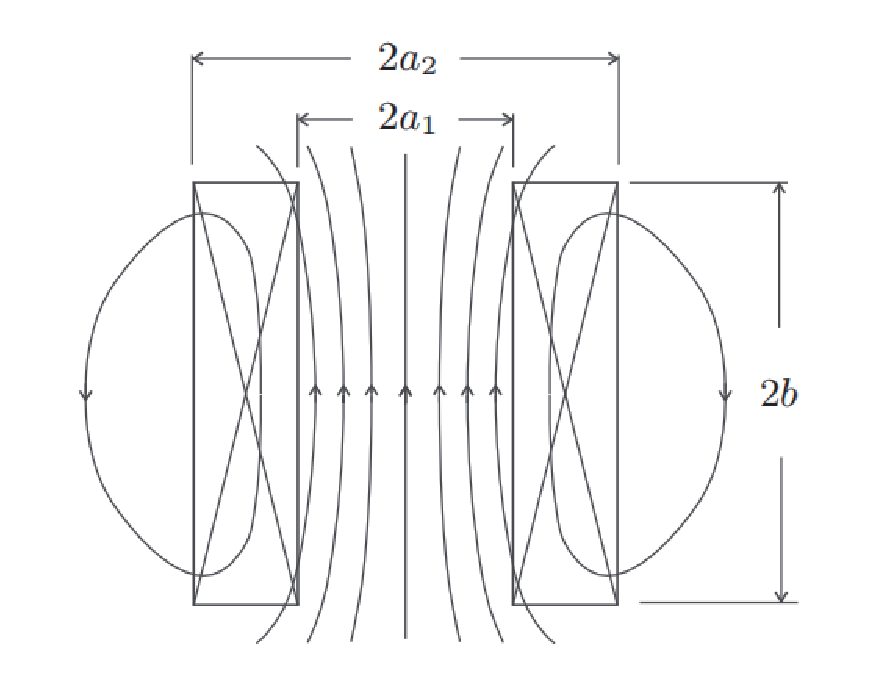
\includegraphics[scale=0.5]{chpt3/figs/fig3.3.eps}
	\caption{内径、外径和长度分别为$2a_1, 2a_2, 2b$的螺管线圈的剖面图。从磁力线可以看出,线圈产生的磁场在室温孔内主要是沿轴向的;除了线圈的对称轴上和轴中平面上,磁力线都是沿径向室温孔外发散的。}
\end{figure}

在如图3.4所示的球坐标系$(r,\theta,\varphi)$下,任何电流体系和/或磁性材料产生的$z$向磁场$H_z(r,\theta,\varphi)$在除源以外空间可以写为:
\begin{equation}\label{eqn:solenoid coil hz}
  H_z (r,\theta,\varphi)=\sum_{n=0}^\infty \sum_{m=0}^n r^n (n+m+1) P_n^m(u)(A_n^m\cos m\varphi+B_n^m\sin m\varphi)
\end{equation}
式中,$\theta$是极角,$\varphi$是周向角,磁场沿$z$向。如第2章所讨论的,$P_n^m(u)$是Legendre多项式($m=0$)和$u=\cos\theta$时的伴随Legendre函数($m>0$)。

$A_n^m$和$B_n^m$是常数。通常除了$A_0^0$和$B_0^0$都需要被最小化的,因为它们会导致磁场的不均匀性。
$A_n^m$和$B_n^m$可以通过调节磁体中各线圈的参数来实现最小化。
这些参数包括线圈内径$2a_1$、外径$2a_2$、长度$2b$、中平面相对于磁体中心的位置、总体电流密度等。
简单说,所有与磁场的空间分布有关的参数都仅仅是上面定义的无量纲参数$\alpha, \beta$的函数。
\begin{figure}[htbp]
	\centering
	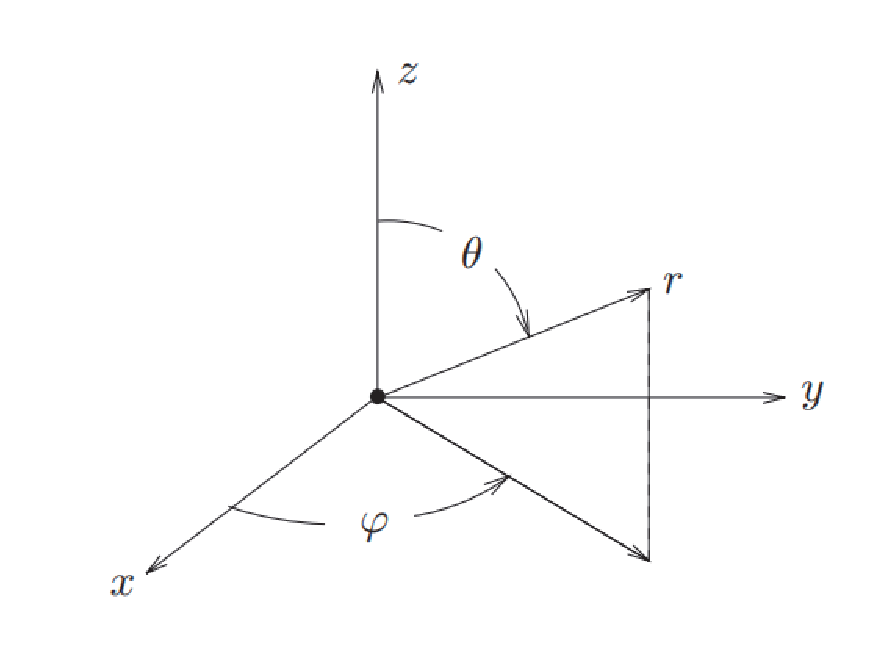
\includegraphics[scale=0.5]{chpt3/figs/fig3.4.eps}
	\caption{圆柱坐标系。}
\end{figure}

由于在螺管系统中所有的电流密度均不随$\varphi$改变,即轴对称,故仅$m=0$项保留。
在$z$轴($r=z,\theta=0$)上可将式3.9简化为:
\begin{subequations}\label{eqn:solenoid coil hz1}
\begin{align}
H_z(z)&=\sum_{n=0}^\infty z^n(n+1)A_n^0 \\
%\mbox{沿$x$(或$y$)轴($x,\theta=90^\circ$),在中平面上式3.9成为:}&\\\nonumber
H_z(x)&=\sum_{n=0}^\infty \sum_{m=0}^n x^n(n+m+1)P_n^m(0)A_n^m
\end{align}
\end{subequations}

式3.10a不含Legendre函数,因为$P_n^0(1)=P_n(1)=1$。
式3.10b中,注意到当$n$为偶数且$m$为奇数时有$ P_n^m(0)=0$。
第2章的表2.3给出了$m$为偶数直到$m=10$的$P_n^m(0)$的数值。
代入$n$和$m=0,2,4$的$P_n^m(0)$值,我们可以写出笛卡尔坐标系下的$H_z(z)$和$H_z(x)$:
\begin{subequations}\label{eqn:solenoid coil hz2}
	\begin{align}
H_z(z)&=A_0^0+3A_2^0z^2+5A_4^0z^4+\cdots\\
H_z(x)&=A_0^0-\left(\frac{3}{2}A_2^0-15A_2^2\right)x^2+\left(\frac{15}{8}A_4^0-\frac{105}{2}A_4^2+945A_4^4\right)x^4+\cdots
\end{align}
\end{subequations}
式中,$A_0^0$是磁体中心$(0,0,0)$的场:$A_0^0\equiv H_0$。
``理想''螺管线圈中,在$m>0$时,系数为0:$A_n^n=0$。
对于$n>0, m=0$时,系数$A_n^0$是线圈参数$\alpha, \beta$的函数。
引入$h_z(\zeta)\equiv H_z(z)/H_0$和$h_z(\xi)\equiv H_z(x)/H_0$,此处$\zeta \equiv z/a_1,\xi\equiv x/a_1$。我们得到:
\begin{subequations}\label{eqn:solenoid coil hz2}
	\begin{align}
h_z(\zeta)=&1+E_2(\alpha,\beta)\xi^2+E_4(\alpha,\beta)\zeta^4\notag\\
&+E_6(\alpha,\beta)\zeta^6++E_8(\alpha,\beta)\zeta^8+E_{10}(\alpha,\beta)\zeta^{10}+\cdots \\
h_z(\xi) =&1-\frac{1}{2}E_2(\alpha,\beta)\xi^2+\frac{3}{8}E_4(\alpha,\beta)\xi^4\notag\\
&-\frac{5}{16}E_6(\alpha,\beta)\xi^6+\frac{35}{128}E_8(\alpha,\beta)\xi^8-\frac{63}{256}E_{10}(\alpha,\beta)\xi^{10}+\cdots
	\end{align}
\end{subequations}

注意到$\xi^2$的系数仅为$\zeta^2$系数的一半(且异号),
$\xi^4$的系数为$\zeta^4$的$3/8$(同号)。
实际上,平面方向的任何系数在数值上都小于$z$向的,所以,$x$和$y$方向场的不均匀性要比$z$向小。

中心场$H_0(\equiv A_0^0)$由下式给出:
\begin{subequations}\label{eqn:h0}
	\begin{align}
  H_0=&\lambda J a_1 F(\alpha,\beta)=\lambda J a_1 \beta \ln \left[\frac{\alpha+\sqrt{\alpha^2+\beta^2}}{1+\sqrt{1+\beta^2}}\right] \\
%\mbox{由式3.13a我们注意到:}\\\notag
  F(\alpha,\beta)=&\beta \ln \left[\frac{\alpha+\sqrt{\alpha^2+\beta^2}}{1+\sqrt{1+\beta^2}}\right]
  	\end{align}
\end{subequations}
式中,$F(\alpha,\beta)$是均匀电流密度线圈的``磁场因子"[3.2]。
上式的衍生问题留到问题3.1中讨论。
式3.12中$E_n (\alpha,\beta)$在$n=2,4,6,8,10$时的表达式在下面以$F(\alpha,\beta)$和$E_n(\alpha,\beta)$的乘积的形式给出[3.3]。除了$2^{th}$阶外,高阶的表达式都使用积分上下限的简洁表达形式:
\begin{subequations}
\begin{align}
F(\alpha,\beta) E_2(\alpha,\beta)=& \frac{1}{2\beta}\left[\frac{1}{(1+\beta^2)^{1.5}}-\frac{\alpha^3}{(\alpha^2+\beta^2)^{1.5}}\right]\\
F(\alpha,\beta)E_4(\alpha,\beta)=&-\frac{r^3}{24\beta^3}\left[\frac{2r^4+7r^2\beta^2+20\beta^4}{(\alpha^2+\beta^2)^{3.5}}\right]\bigg|_{r=1}^{r=\alpha}\\
F(\alpha,\beta)E_6(\alpha,\beta)=&-\frac{r^3}{240\beta^5}\left[\frac{8r^8+44 r^6\beta^2+99 r^4\beta^4+28 r^2 \beta^6+280 \beta^8}{(r^2+\beta^2)^{5.5}}\right]\bigg|_{r=1}^{r=\alpha}\\
F(\alpha,\beta)E_8(\alpha,\beta)=&-\frac{r^3}{896\beta^7}\bigg[\bigg(16 r^{12}+120 r^{10}\beta^2+390r^8\beta^4+715r^6\beta^6\notag\\
&+1080r^4\beta^8-1008r^2\beta^{10}+1344\beta^{12}\bigg)/(r^2+\beta^2)^{7.5}\bigg]\bigg|_{r=1}^{r=\alpha}
\end{align}
\end{subequations}

$F(\alpha,\beta)E_{n}(\alpha,\beta)$是一个递归式;第$n$阶项可由下式导出:
\begin{subequations}
	\begin{align}
F(\alpha,\beta)E_{n}(\alpha,\beta)&=\frac{1}{n} \frac{\partial}{\partial \beta}\left[F(\alpha=1,\beta)E_{n-1}(\alpha=1,\beta)-F(\alpha,\beta)E_{n-1}(\alpha,\beta)\right]\\
F(\alpha,\beta) E_{n}(\alpha,\beta)&=\frac{1}{M_n \beta^{n-1}}\left[\frac{f_n(\alpha=1,\beta)}{(1+\beta^2)^{n-0.5}}-\frac{\alpha^3 f_n(\alpha,\beta)}{(\alpha^2+\beta^2)^{n-0.5}}\right]
\end{align}
\end{subequations}
式中,$M_n$是一个常数。例如,由式3.14a、3.14b和3.15b我们找到:$f_2(\alpha,\beta)=1,M_2=2$以及
$f_4(\alpha,\beta)=2\alpha^4+7\alpha^2\beta^2+20\beta^4,M_4=24$。
附录IB给出了$n=2,3,4,...20$时的$M_n$值和$f_n(\alpha,\beta)$表达式。
20之下的偶数$n$对应的$f_n$常用来求解磁场问题。

根据上面的讨论(式3.12a和式3.12b),磁场$H_z(z)$的均匀性要比$z$轴法平面上的磁场$H_z(x),H_z(y)$均匀性差(也不尽然,比如嵌套线圈磁体)。因而,我们仅考虑$z$轴向磁场。根据式3.12a,可写出对应形式以及一般形式:
\begin{subequations}
	\begin{align}
\frac{\partial^2 h_z(\zeta)}{\partial \zeta^2}=&[2 E_2(\alpha,\beta)+(4)(3)E_4(\alpha,\beta)\zeta^2+...]\nonumber\\
&=\sum_{n=1}^{\infty} (2n)(2n-1)E_{2n}(\alpha,\beta)\zeta^{2(n-1)}\\
 \frac{\partial^{2k} h_z(\zeta)}{\partial \zeta^{2k}}=&\sum_{n=k}^{\infty} (2n)(2n-1)(\cdots)(2n-2k+1)E_{2n}(\alpha,\beta)\zeta^{2(n-k)}
	\end{align}
\end{subequations}

在原点处,$\zeta=0$。式3.16a和3.16b由于仅第一项非零,可以化简为:
\begin{subequations}
	\begin{align}
\frac{\partial^2 h_z(\zeta)}{\partial \zeta^2}\bigg|_{0}&=2 E_{2}(\alpha,\beta)\\
\frac{\partial^{2k} h_z(\zeta)}{\partial \zeta^{2k}}\bigg|_{0}&=(2k)! E_{2k}(\alpha,\beta)
	\end{align}
\end{subequations}

\subsubsection{嵌套线圈磁体}
对一个由$\ell$个线圈嵌套(同心且同轴,各线圈参数均为$\lambda J, a_1, \alpha, \beta$)组成的磁体,
式3.12a仅给至$\zeta^2$项可一般地写为:
\begin{equation}
  h_z(\zeta)=1+\frac{\sum_{j=1}^{\ell} (\lambda J)_j a_{1_j}F(\alpha_j,\beta_j)E_2(\alpha_j,\beta_j)}{\sum_{j=1}^{\ell}(\lambda J)_j a_{1_j} F(\alpha_j,\beta_j)}\zeta^2+\cdots
\end{equation}

在3.4.2节讨论两线圈嵌套磁体误差前,我们首先考虑几个单螺管线圈的特例。

\subsection{简单线圈}
本节我们推导``简单"线圈的$E_n(\alpha,\beta)$和$h_z(\zeta)$在$10^{th}$阶以下的表达式。
各$h_z(\zeta)$表达式可以给设计者在不依赖磁场分析专家的情况下,
``感受''待设计线圈的尺寸(即$\alpha, \beta$)对线圈的磁场均匀性的影响。

\subsubsection{``短"线圈}
对于短线圈($\beta\rightarrow 0 $),如饼式线圈,$F(\alpha,\beta)$可简化为:
\begin{equation}
  F(\alpha,\beta\rightarrow 0)=\beta \ln\alpha
\end{equation}

虽然推导过程\textit{极端}枯燥,最终可从式3.14中得出$E_2(\alpha,0),\cdots,E_{10}(\alpha,0)$。
在$\beta\rightarrow 0$极限下,$f_n(\alpha,\beta)$各项的分母$(1+\beta^2)^{n-0.5}$可以展开
为$\beta^{2k}$的幂级数直到$\beta^n$项,其中整数$k$取遍$1$至$n/2$。
\begin{equation}
 \frac{1}{(1+\beta^2)^{n-0.5}}=1-(n-0.5)(n+0.5)\frac{\beta^4}{2!}-\cdots+(-1)^k (n-0.5)(n+0.5)\cdots(n+k-1.5)\frac{\beta^{2k}}{k!}
\end{equation}

在$\beta\rightarrow 0$极限下,式3.20等号右侧高于$\beta^n$的项为相比$\beta^n$的高阶小,可忽略。
同时,所有小于$\beta^n$的项都被约掉,仅剩下含$\beta^n$的项。

由式3.14和3.19导出的$E_n(\alpha,0)$可写为:
\begin{subequations}
	\begin{align}
  E_2(\alpha,0) &= -\frac{3(\alpha^2-1)}{4\alpha^2 \ln \alpha} \\ 
  E_4(\alpha,0) &= \frac{15(\alpha^4-1)}{32\alpha^4 \ln \alpha} \\ 
  E_6(\alpha,0) &= -\frac{35(\alpha^6-1)}{96\alpha^6\ln \alpha} \\ 
  E_8(\alpha,0) &= \frac{315(\alpha^8-1)}{1024\alpha^8 \ln \alpha} \\
    E_{10}(\alpha,0) &= -\frac{693(\alpha^{10}-1)}{2560\alpha^{10} \ln \alpha}
    \end{align}
\end{subequations}

式3.12a于是成为:
\begin{align}
  h_z(\zeta)=1&-\frac{3(\alpha^2-1)}{4\alpha^2 \ln \alpha}\zeta^2+\frac{15(\alpha^4-1)}{32\alpha^4 \ln \alpha}\zeta^4 -\frac{35(\alpha^6-1)}{96\alpha^6\ln \alpha}\zeta^6\\\notag
  &+\frac{315(\alpha^8-1)}{1024\alpha^8\ln \alpha}\zeta^8-\frac{693(\alpha^{10}-1)}{2350\alpha^{10}\ln \alpha}\zeta^{10}+\cdots
\end{align}

\subsubsection{``薄壁"线圈}
对于``薄壁"线圈($\alpha=1$),$F(\alpha,\beta)$成为:
\begin{subequations}
\begin{align}
  \lim_{\alpha\rightarrow 1} F(\alpha,\beta)&=\beta\frac{\epsilon}{\sqrt{1+\beta^2}}\\
  &=\frac{\beta(\alpha-1)}{\sqrt{1+\beta^2}}
\end{align}
\end{subequations}

联立式3.14和6.23,可得$E_n(1,\beta)$的表达式:
\begin{subequations}
\begin{align}
E_2(1,\beta) &=-\frac{3}{2(1+\beta^2)^2} \\ 
E_4(1,\beta) &= \frac{5(3-4\beta^2)}{2^3(1+\beta^2)^4} \\ 
E_6(1,\beta) &= -\frac{7(5-20\beta^2+8\beta^4)}{2^4 (1+\beta^2)^6} \\
E_8(1,\beta) &= \frac{9(35-280\beta^2+336\beta^4-64\beta^6)}{2^7(1+\beta^2)^8} \\ E_{10}(1,\beta) &= -\frac{11(63-840\beta^2+2016\beta^4-1152\beta^6+128\beta^8)}{2^8(1+\beta^2)^{10}}
\end{align}
\end{subequations}

于是,对于``薄壁"线圈,我们有:
\begin{equation}
  h_z(\zeta)=1-\frac{3}{2(1+\beta^2)^2}\zeta^2 +\frac{5(3-4\beta^2)}{8(1+\beta^2)^4}\zeta^4-\frac{7(5-20\beta^2+8\beta^4)}{16(1+\beta^2)^6}\zeta^6+\cdots
\end{equation}

\subsubsection{``薄壁且长"线圈}
对于``薄壁且长"线圈($\alpha=1,\beta\rightarrow \infty$),式3.25简化为:
\begin{equation}
  h_z(\zeta)=1-\frac{1.5}{\beta^4}\zeta^2-\frac{2.5}{\beta^6}\zeta^4-\frac{3.5}{\beta^8}\zeta^6-\cdots-\frac{n+1}{2\beta^{n+2}}\zeta^{n}
\end{equation}

从式3.26可知,在$\beta\rightarrow \infty$极限下,$E_n(1,\beta)=-(n+1)/2\beta^{(n+2)}$。
正如我们所预期的,随线圈长度增加,均匀度提高。

\subsubsection{``环"线圈}
对``环"线圈($\alpha=1,\beta=0$),$E_n(\alpha,\beta)$可由式3.21在极限$\alpha=1$导出,
或由式3.25在极限$\beta=0$下导出。在式3.21中,
\begin{equation}
  \lim_{\alpha\rightarrow 1}\frac{\alpha^n-1}{\alpha^n \ln\alpha}=n
\end{equation}

于是,我们可以通过联立式3.21和3.27,或者简单的在式3.24中令$\beta=0$,都可得同样结果:
\begin{subequations}
\begin{align}
E_2(1,0) =& -\frac{3}{2}=-1.5 \\ 
E_4(1,0) =& \frac{3\cdot 5}{2^3}=1.875 \\ 
E_6(1,0) =& -\frac{3\cdot 5 \cdot 7}{2\cdot 4\cdot 6}\simeq-2.188 \\ 
E_8(1,0) =&\frac{3\cdot 5 \cdot 7\cdot 9}{2\cdot 4\cdot 6\cdot 8}\simeq 2.461 \\ 
E_{10}(1,0) =-&\frac{3\cdot 5 \cdot 7\cdot 9\cdot 11}{2\cdot 4\cdot 6\cdot 8\cdot 10}\simeq -2.707
\end{align}
\end{subequations}

于是,``环"线圈的$h_z(\zeta)$为:
\begin{equation}
  h_z(\zeta)=1-1.5\zeta^2+1.875\zeta^4-2.188\zeta^6+2.461\zeta^8-2.707\zeta^{10}+\cdots
\end{equation}

问题3.4中,将通过式3.124诸式给出$E_{12}(1,0),E_{14}(1,0),E_{16}(1,0),E_{18}(1,0),E_{20}(1,0)$的值。

\subsection{谐波误差—嵌套双线圈磁体}
式3.12a和3.12b表明,$h_z(\zeta)$和$h_z(\xi)$(其中,$h_z(\zeta)\equiv H_z/H_0,\zeta\equiv z/a_1,\xi\equiv x/a_1$)都仅与$\zeta$或$\xi$的偶次幂有关。
也即,两式都表出了``理想"螺管或者此种螺管的``理想"嵌套组合的轴向场的空间变化。
在这里,``理想"一词指的是空间对称性、均匀性以及电流密度的不变性。

哪怕对单螺管,在现实中也是很不同的,例如线圈形状的不完美;导体的尺度和形状不一致;导体的移位。
这会引起磁场中不只存在偶次幂。
如果一个磁体是由嵌套线圈组成的,可能的不完美就更多了,会出现很多``不希望"的谐波项。
下面,我们将展给出嵌套双线圈磁体谐波误差的起源。

考虑一个双螺管线圈嵌套磁体:参数为$[2a_1]_1,\alpha_1,\beta_1,[\lambda J]_1$的螺管线圈1嵌入参数为$[2a_1]_2,\alpha_2,\beta_2,[\lambda J]_2$的螺管线圈2的室温孔内。
如果两个线圈在轴向和径向都对齐的话,有:
\begin{equation}
H_z(z)=[H_z(z)]_1+[H_z(z)]_2
\end{equation}
根据式3.11a,式中的$[H_z(z)]_1$和$[H_z(z)]_2$可写为:
\begin{subequations}
	\begin{align}
  [H_z(z)]_1 &= [A_0^0]_1 +3[A_2^0]_1 z^2+5[A_4^0]_1 z^4+... \\ 
  [H_z(z)]_2 &= [A_0^0]_2 +3[A_2^0]_2 z^2+5[A_4^0]_2 z^4+...
  \end{align}
\end{subequations}

注意到,中心的总轴向场有:$H_z(0)=[A_0^0]_1+[A_0^0]_2\equiv H_0$

\subsubsection{线圈轴向失配}
如果线圈1和线圈2在径向是对齐的(即同轴),但其中平面未对齐,分别在$z=0$和$z=\delta_z$位置。
这样,式3.31中的$H_z(z)$成为3.32a。若将3.32a按$z$合并同类项,有3.32b。
\begin{subequations}
	\begin{align}
  H_z(z)=&H_0+3\{ [A_2^0]_1 z^2+[A_2^0]_2(z-\delta_z)^2\}+5\{[A_4^0]_1 z^4+[A_4^0]_2(z-\delta)^4\}+\cdots\\
H_z(z)=&\{H_0+3[A_2^0]_2 \delta_z^2+5[A_4^0]_2\delta_z^4+\cdots\}-\{6[A_2^0]_2\delta_z+20[A_4^0]_2\delta_z^3+\cdots\}z\nonumber\\
&+\{3[A_2^0]_1+3[A_2^0]_2+30[A_4^0]_2\delta_z^2+\cdots\}z^2-\{20[A_4^0]_2\delta_z+\cdots\}z^3\notag\\
&+\{5[A_4^0]_1+5[A_4^0]_2+\cdots\}
\end{align}
\end{subequations}

从式3.32b可以看出,线圈1和线圈2在轴向失配$\delta_z$不仅影响了各$z$偶次项的系数,
更重要的是还增加了$z$的奇次幂项,这将导致$H_z(z)$在轴向不再对称。

在\textit{实际}的由许多线圈嵌套组成的NMR磁体中,轴向失配是不可避免的。
具体而言,$z$项要么扩大NMR谱线,要么引起谱线中各峰值的``下沉"。
$z^3$项同样扩大了谱线,主要是在偏离中心频率之处。

\subsubsection{轴向补偿线圈}
那些``不希望"的谐波项可以通过在超导磁体的校正线圈外再增加补偿线圈来消减;
甚至,补偿线圈还可以布置在探测器和低温容器室温孔之间的径向间隙中。

最小化$z$偶次幂项的补偿线圈主要是``Helmholtz"线圈,其基本特性我们将在问题3.3中研究;
最小化$z$奇次幂项的补偿线圈同样是Helmholtz型的,但其中一个线圈是反极性的,以产生轴向反对称场。

\subsubsection{线圈径向失配}
为了研究径向失配的嵌套双线圈磁体的磁场的空间变化,我们首先在笛卡尔坐标系中写出单螺管的$H_z(x,y,z)$。
根据式3.11和表2.4中$n=0,n=2,n=4$的Legendre函数,可得3.33a式。当线圈2与线圈1在径向失配,具体为在$x$方向失配$\delta_x$,在$y$方向失配$\delta_y$。我们将式3.33a中的$x$和$y$分别用$x-\delta_x$和$y-\delta_y$替换,有3.33b式。
\begin{subequations}
	\begin{align}
  H_z(x,y,z)=&A_0^0+3A_2^0[z^2-\frac{1}{2}(x^2+y^2)]+5A_4^0\left\{z^4-3(x^2+y^2)\left[z^2-\frac{1}{8}(x^2+y^2)\right]\right\}\\
H_z(x,y,z)=&H_0+3\left([A_2^0]_1\left[z^2-\frac{1}{2}(x^2+y^2)\right]+[A_2^0]_2\left\{ z^2-\frac{1}{2}\left[(x-\delta_x)^2+(y-\delta_y)^2\right]\right\}\right)\\\notag
&+5[A_4^0]_1\left(z^4-3(x^2+y^2)\left[z^2-\frac{1}{8}(x^2+y^2)\right]\right)\\\notag
&+[A_4^0]_2\left(z^4-3\left[(x-\delta)^2+(y-\delta_y)^2\right]\left\{ z^2-\frac{1}{8}\left[(x-\delta_x)^2+(y-\delta_y)^2\right]\right\}\right) 
\end{align}
\end{subequations}

式3.33b的展开式包含很多项,包括$x,x^2,x^3,x^4,y,y^2,y^3,y^4,xy,xy^2,z^2,z^2x,\cdots$等。

一个$x$向补偿线圈通常由一对薄的(一层或几层导体厚)成型为``鞍状"以适应磁体的外圆柱表面并且其轴向沿$\varphi=0(x)$方向布置的长方形线圈构成。
它产生一个随$x$增大的$z$向磁场,在$z$轴($x=0$)处为0。
类似的,$y$向补偿线圈和$xy$补偿线圈分别是沿着$\varphi=90^\circ$和$\varphi=45^\circ$轴成对布置。
每个线圈产生一个$z$向、随远离$z$轴而增大的磁场。

\subsubsection{线圈轴向和径向均失配}
当嵌套线圈在轴向和径向均失配的时候---实际NMR中不可避免---将产生$xz,yz,xyz$及其他更多的谐波误差。

\section{轴向力}
本节给出轴向对齐``环"线圈、``薄壁''螺管线圈等的轴向力$F_z$的解析表达式,
这些表达式都是从Garrett [3.5]最早给出的原始表达式推导得到的。
极限情况下(比如相距很远的线圈)的近似表达式可用于快速的数值检查;
另一些公式可作为写自编计算程序的基准。
所有案例均假定电流同向流动;任一电流反向,将导致力的反向。

\subsection{两个``环"线圈间的轴向力}
\begin{figure}[htbp]
	\centering
	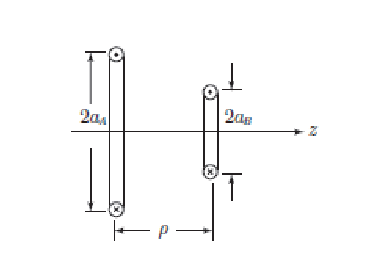
\includegraphics[scale=1]{chpt3/figs/fig3.5.eps}
	\caption{``环"线圈A和B同轴对齐,距离上相距$\rho$}
\end{figure}
图3.5给出了沿轴向($\vec{i}_z$)放置的两个距离为$\rho$的``环"线圈($\alpha=1,\beta=0$)。
线圈A和B的直径分别为$2a_A$和$2a_B$,总安匝数分别为$N_A I_A$和$N_B I_B$。
两线圈产生的轴向($\vec{i}_z$)场指向同一方向。
线圈B施加给线圈A的轴向力$F_{zA}(\rho)$为:
\begin{align}
  F_{zA}(\rho)=\frac{\mu_0}{2}(N_A I_A)(N_B I_B)\frac{\rho\sqrt{(a_A+a_B)^2+\rho^2}}{(a_A-a_B)^2+\rho^2}\times\left\{k^2 K(k)+(k^2-2)[K(k)-E(k)]\right\}
\end{align}

$F_{zA}(\rho)$的方向为$+z$,或指向线圈B的;也即,$F_{zA}(\rho)$是引力。
若两个电流的方向相反,则符号变为$-$,$F_{zA}(\rho)$成为斥力。
式3.34中,$K(k)$和$E(k)$分别是第一类和第二类完全椭圆积分,定义为:
\begin{subequations}
	\begin{align}
  K(k) &= \int_{0}^{\pi/2} \frac{d\theta}{\sqrt{1-k^2\sin^2\theta}} \\
  E(k)&= \int_{0}^{\pi/2}\sqrt{1-k^2 \sin^2\theta}d\theta
  \end{align}
\end{subequations}
本系统中椭圆积分的模量$k$由下式决定:
\begin{equation}
  k^2=\frac{4a_A a_B}{(a_A+a_B)^2+\rho^2}
\end{equation}

%%%%%%%%表格3.1
\begin{table}[htbp]\small
\centering
\caption{第一类和第二类完全椭圆积分参数:部分$k^2$和$k$下的$K(k)$和$E(k)$值}
\label{my-label}
\begin{tabular}{|c|c||c|c||c|c||c|c|}
\hline
$k^2$    & $k$  & $K(k)$ &$E(k)$  &$k^2$  & $k$ &$K(k)$  &$E(k)$  \\ \hline\hline
0   & 0 &$\pi/2$  & $\pi/2$ &0.7&0.8367  &2.0754  & 1.2417 \\ 
0.1 & 0.3162  & 1.6124 &1.5308  &0.8& 0.8944 & 2.2572 & 1.1785 \\ 
0.2 & 0.4472  & 1.6596 &1.4890  &0.9&0.9487  & 2.5781 & 1.1048 \\ 
0.3 & 0.5477  & 1.7139 & 1.4454 &0.95&0.9747  &2.9083  & 1.0605 \\
0.4 & 0.6325  & 1.7775 &1.3994  &0.98& 0.9899 & 3.3541 & 1.0286 \\ 
0.5 & 0.7071  & 1.8541 &1.3506  & 0.99& 0.9950 &3.6956  & 1.0160 \\ 
0.6 & 0.7746  & 1.9496 &1.2984  &1  &1  &$\infty$  &  1\\ \hline
\end{tabular}
\end{table}

表3.1给出了部分$k$和$k^2$值下的$K(k)$和$E(k)$。我们发现,$K(0)=E(0)=\pi/2$;以及$K(1)=\infty$以及$E(1)=1$,也即$K(k)$随$k$增加而增加,$E(k)$随k增加而减小。
例如,如果$k^2=0.5$,$K(k=0.7071)=1.8541$。

$K(k)$和$E(k)$可展开为$k^2$的幂级数:
\begin{subequations}
	\begin{align}
  K(k) =& \frac{\pi}{2}\left[1+\left(\frac{1}{2}\right)^2 k^2+\left(\frac{1\cdot 3}{2\cdot 4}\right)^2 k^4+\left(\frac{1\cdot 3\cdot 5}{2\cdot 4\cdot 6}\right)^2 k^6+\cdots\right] \\
  E(k) =& \frac{\pi}{2}\left[1-\left(\frac{1}{2}\right)^2 k^2-\left(\frac{1\cdot 3}{2\cdot 4}\right)^2 \frac{k^4}{3}-\left(\frac{1\cdot 3\cdot 5}{2\cdot 4\cdot 6}\right)^2 \frac{k^6}{5}-\cdots\right]
 	\end{align}
  \end{subequations}

在$k^2\ll 1$时,两个积分及其差值可近似为:
\begin{subequations}
	\begin{align}
  K(k) \simeq&  \frac{\pi}{2}\left(1+\frac{1}{4}k^2+\frac{9}{64}k^4+\frac{25}{256}k^6+\frac{1225}{16384}k^8\right)\\
  E(k) \simeq&  \frac{\pi}{2}\left(1-\frac{1}{4}k^2-\frac{3}{64}k^4-\frac{5}{256}k^6-\frac{175}{16384}k^8\right)\\ 
  K(k)-E(k) \simeq& \frac{\pi}{4}\left(k^2+\frac{3}{8}k^4+\frac{15}{64}k^6+\frac{175}{1024}k^8\right) 
  	\end{align}
\end{subequations}

\subsubsection{特例1:两个距离很远``环"线圈}
当两个线圈距离足够远,即$\rho^2 \gg (a_A+a_B)^2$时,有$k^2\ll 1$。
此时,可以用式3.38a和3.38c来简化式3.34。式3.34第一步可简化为:
\begin{equation}
  F_{zA}(\rho)\simeq \frac{\mu_0}{2}(N_A I_A)(N_B I_B)\left\{ k^2K(k)+(k^2-2)[K(k)-E(k)]\right\}
\end{equation}

接下来,用式3.38a和3.38c。尽管$k^2\ll 1$,但展开$K(k)-E(k)$时必须考虑$k^4$项,
因为与它相乘的,除了$k^2$还有$-2$:
\begin{align*}
F_{zA}(\rho)\simeq&\frac{\mu_0}{2}(N_AI_A)(N_BI_B)\times\left[k^2\left(\frac{\pi}{2}+\frac{\pi}{8}k^2\right)+(k^2-2)\left(\frac{\pi}{4}k^2+\frac{3\pi}{32}k^4\right)\right]\\
\simeq& \frac{\mu_0}{2}(N_A I_A)(N_B I_B)\left(\frac{3\pi}{16}k^4\right) \tag{3.39b}
\end{align*}

第二步近似时,忽略$k^6$项。
最终,我们得到在极限$\rho^2 \gg (a_A+a_B)^2$时,力的简单表达式:
\begin{equation*}
F_{zA}(\rho)= \frac{3\mu_0}{2\pi}\left(\frac{\pi a_A^2 N_A I_A}{\rho^2}\right)\left(\frac{\pi a_B^2 N_B I_B}{\rho^2}\right) \tag{3.39c}
\end{equation*}

式3.39c表明,轴向力正比于两线圈各自``磁矩''($\pi a_A^2 N_A I_A$和$\pi a_B^2 N_B I_B$)比距离$\rho^2$之乘积。讨论3.17中,我们将从互感表达式中再次导出3.39c式。

\subsubsection{特例2:两个距离很近且直径相同的``环"线圈}
如果两个环线圈的直径相同且距离很近,即$a_A=a_B=a$以及$\rho\ll 2a$。
于是,$k^2\rightarrow 1,K(k)\rightarrow\infty,E(k)\rightarrow 1$。
此时,式3.34可以有更简单的形式:
\begin{equation*}
F_{zA}(\rho)\simeq \mu_0(N_A I_A)(N_B I_B)\left(\frac{a}{\rho}\right) \tag{3.39d}
\end{equation*}

我们可以式3.39d表示为``环"线圈A直径($2\pi a$)、安匝($N_A I_A$)和轴向$\rho$处的``环"线圈B在``环"线圈A处产生的磁场的径向分量($B_r$)的乘积。
由于$\rho\ll a$,两线圈可视为两条距离为$\rho$的直线,于是磁场可近似为$\mu_0 N_B I_B/(2\pi\rho)$。于是:
\begin{align*}
F_{zA}(\rho)&\simeq (2\pi a)\times(N_A I_A)\times\left(\frac{\mu_0 N_B I_B}{2\pi\rho}\right)\\
&=\mu_0(N_A I_A)(N_B I_B)(\frac{a}{\rho}) \tag{3.39d}
\end{align*}


\subsection{``薄壁"螺管内的轴向力}
考虑一个直径为$2a$,长度为$2b$,中平面位于$z=0$,通以$NI/2b$均匀表面电流的``薄壁''($\alpha=1$)螺管线圈。
该螺线管中距中平面$z\ge 0$处的轴向力可以表示为:
\begin{align}
F_z(z)=-\frac{\mu_0}{2}\left(\frac{NI}{2b}\right)^2&\bigg\{(b-z)\sqrt{4a^2+(b-z)^2}\left[K(k_{b_-})-E(k_{b_-})\right]\\\notag
&+(b+z)\sqrt{4a^2+(b+z)^2}\left[K(k_{b_+})-E(k_{b_+})\right]\\\notag
&-2b\sqrt{4a^2+4b^2}\left[K(k_{2b})-E(k_{2b})\right]\bigg\}
\end{align}
式中的椭圆积分模量分别为:
$$k_{b_-}^2=\frac{4a^2}{4a^2+(b-z)^2} ; \quad k_{b_+}^2=\frac{4a^2}{4a^2+(b+z)^2} ;\quad k_{2b}^2=\frac{4a^2}{4a^2+4 b^2}$$

\subsubsection{特例3:端部力}
在$z=b$处,因为$k_{b_+}=k_{2b}$,根据式3.40,有$F_z(b)=0$。
即一个孤立螺线管端部的轴向力是零,这和我们的预期一致。

\subsubsection{特例4:中平面的力}
将$z=0$代入3.40式,可得中平面($z=0$)处的轴向力$F_z(0)$:
\begin{align}
  F_z(0)=-\frac{\mu_0}{2}\left(\frac{NI}{2b}\right)^2&\bigg\{2b\sqrt{4a^2+b^2}\left[K(k_{b})-E(k_{b})\right]\\\notag
  &-2b\sqrt{4a^2+4b^2}\left[K(k_{2b})-E(k_{2b})\right]\bigg\}
\end{align}
式中,模量$k_{2b}$同上;$k_{b}$由下式给出:
$$k_{b}^2=\frac{4a^2}{4a^2+b^2}$$

可见,孤立螺线管沿$z$的轴向\textit{压缩力}在$z=b$为$0$,向内逐渐增大,至中平面处取得最大。

\subsubsection{特例5:``长''薄壁螺管的中平面的力}
对于一个``长"($\beta\gg 1$或者$k^2\ll 1$)的薄壁螺线管,可利用式3.38c将式3.41化简:
\begin{equation*}
F_z(0)\simeq-\frac{\mu_0}{2}\left(\frac{NI}{2b}\right)\pi a^2 \tag{3.41b}
\end{equation*}

式3.41b表明,$F_z(0)$在给定的表面电流密度$NI/2b$下,与线圈长度\textit{无关}。
因为对长螺管的轴向中心场(问题3.1),有$NI/2b=H_z(0,0)$。由此可得:
\begin{equation*}
F_z(0)\simeq -\frac{1}{2}\mu_0 H_z^2(0,0)\times\pi a^2  \tag{3.41c}
\end{equation*}

于是,$F_z(0)$等于磁压乘上线圈室温孔的面积。
实际上,后面我们将看到,\textit{每一个}轴向力的表达式都含有一个磁压项($\mu_0(NI/2b)^2$)或其等价形式。

\subsection{``薄壁"螺管和``环"线圈间的轴向力}
图3.6的``薄壁"螺管($2a_s,2b_s,N_s I_s/2b_s$)与``环"线圈($2a_R,N_R I_R$)同轴。
螺管右端距离环线圈左侧距离为$\rho$。
两线圈产生的轴向场指向同一方向。
螺线管受到的轴向力为:
\begin{align}
F_{zS}(\rho)=&-\frac{\mu_0}{2}\left(N_R I_R\right)\left(\frac{N_S I_S}{2b_s}\right)\times\\\notag
&\bigg(\sqrt{(a_R+a_S)^2+(\rho+2b_s)^2}\{2[K(k_s)-E(k_s)]-k_s^2K(k_s)\}\\\notag
&-\sqrt{(a_R+a_s)^2+\rho^2}\left\{2[K(k_R)-E(k_R)-k_R^2K(k_R)]\right\}\bigg)
\end{align}
式中,模量$k_S$和$k_R$为:
$$k_{S}^2=\frac{4a_S a_R}{(a_S+a_R)^2+(2b_S+\rho)^2} ;\qquad k_{R}^2=\frac{4a_S a_R}{(a_S+a_R)^2+\rho^2} $$

式3.42等号右侧的第二项大于第三项,所以$F_{zS}(\rho)$是正值,即轴向力是引力。

\begin{figure}[htbp]
	\centering
	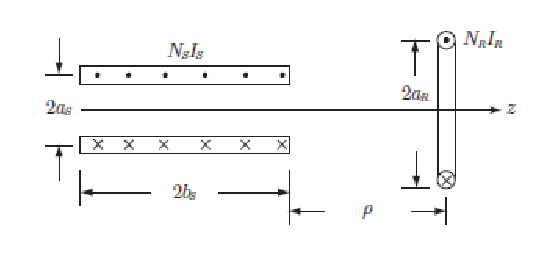
\includegraphics[scale=1]{chpt3/figs/fig3.6.eps}
	\caption{``薄壁"螺管($2a_S,2b_S,N_S I_S/2b_S$)与``环"线圈($2a_R,N_R I_R$)同轴,相距$\rho$。}
\end{figure}

\subsubsection{特例6:相距很远的``薄壁"螺管和``环"线圈}
当两个线圈相距很远可满足$k_s^2\ll 1$和$k_R^2\ll 1$时,可得:
\begin{equation}
F_{zS}(\rho)\simeq \frac{\mu_0}{2\pi}\left(\pi a_R^2N_R I_R\right)\left(\frac{\pi a_S^2 N_S I_S}{2 b_S}\right)\left[\frac{1}{\rho^3}-\frac{1}{(\rho+2b_S)^3}\right]
\end{equation}

和上面的例子类似,力是$+z$向(朝向``环''线圈),幅值正比于两个线圈``磁矩''的乘积。

\subsubsection{特例7:相距极远的``薄壁"螺管和``环"线圈}
当两个线圈的相距足够远可满足$\rho \gg 2b_S$时,对式3.43中的方括号中的做泰勒展开,可略去高次项。此时有:
\begin{equation*}
F_{zS}(\rho)\simeq\frac{\mu_0}{2\pi}(\pi a_R^2 N_R I_R)\left(\frac{\pi a_S^2 N_S I_S}{2 b_S}\right)\frac{6b_S}{\rho^4} \tag{3.43b}
\end{equation*}

不出所料,式3.43b等价于式3.39c。

\subsection{两个``薄壁"螺管间的轴向力}
\begin{figure}[htbp]
  \centering
 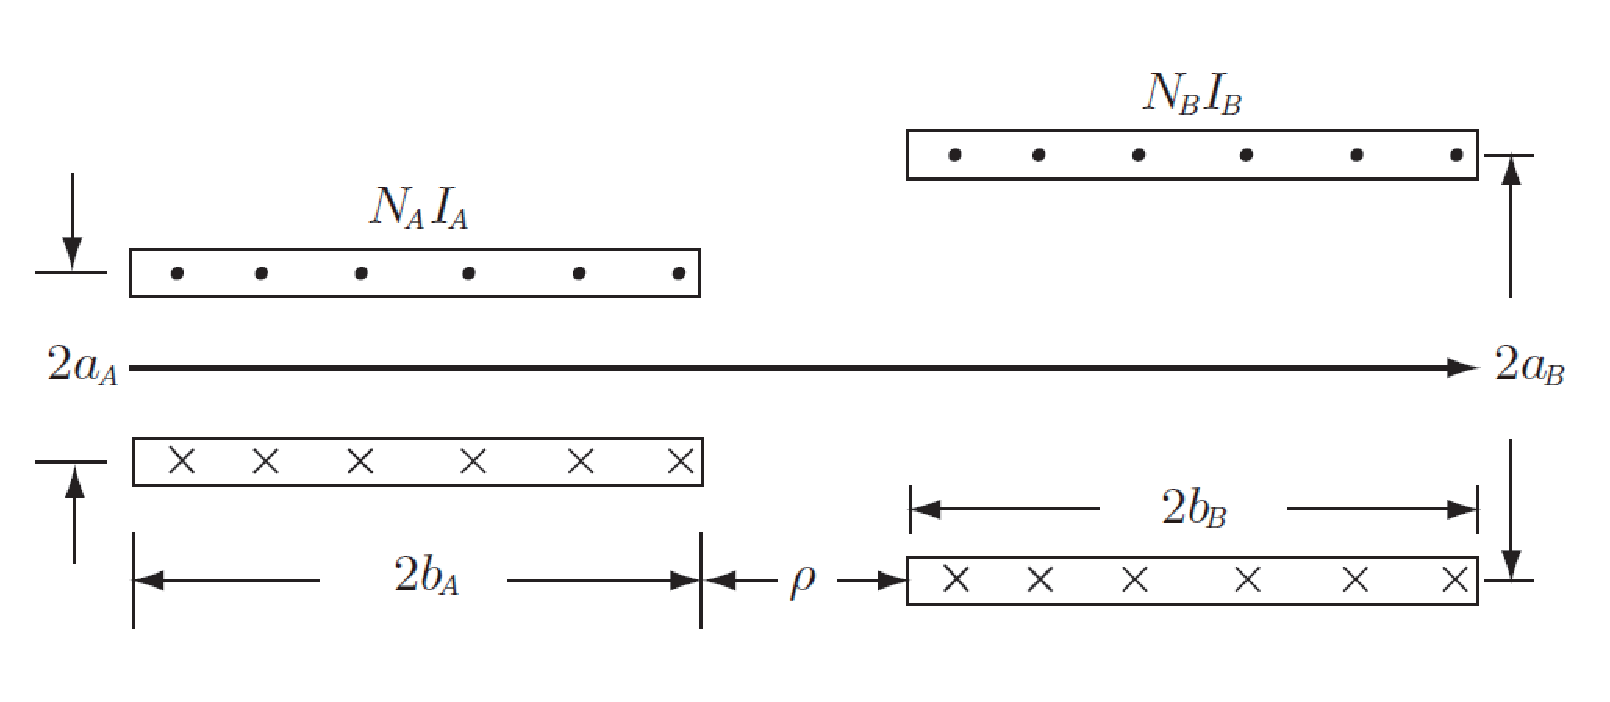
\includegraphics[scale=0.4]{chpt3/figs/fig3.7.eps}
  \caption{``薄壁"螺管A和B,两个最近端相距为$\rho$。}
\end{figure}

本节,我们推导两个``薄壁"螺管之间的轴向力;推导基于Garrett [3.5]方程,但比他走的更远。
这个式子是非``薄壁"的一般性螺管线圈轴向力的基础(3.5.5节)。

考虑两个同轴的``薄壁"螺管线圈A($2a_A; 2b_A; N_A I_A/2b_A$)和B($2a_B; 2b_B;
N_B I_B/2b_B$)。如图3.7所示,螺管A的右端距离螺管B的左端距离为$\rho$。
两螺管线圈产生的轴向场指向同一方向。

\subsubsection{螺管A受到螺管B的轴向力}
螺管B施加给螺管A的轴向力可以写为:
\begin{equation}
\begin{split}
F_{zAB}(\rho)=&\frac{\mu_0}{2}\left(\frac{N_A I_A}{2b_A}\right)\left(\frac{N_B I_B}{2b_B}\right)\times \\
&\bigg(\frac{2b_A+\rho}{\sqrt{a_T^2+(2B_a+\rho)^2}} \{[a_T^2+(2b_A+\rho)^2][K(k_{A})-E(k_{A})]-\Upsilon(c^2,k_A)\}\\
&+\frac{2b_B+\rho}{\sqrt{a_T^2+(2B_B+\rho)^2}} \{[a_T^2+(2b_B+\rho)^2][K(k_{B})-E(k_{B})]-\Upsilon(c^2,k_B) \}\\
&-\frac{2b_T+\rho}{\sqrt{a_T^2+(2B_T+\rho)^2}} \{[a_T^2+(2b_T+\rho)^2][K(k_{T})-E(k_{T})]-\Upsilon(c^2,k_T) \}\\
&-\frac{\rho}{\sqrt{a_T^2+\rho^2}}\{(a_T^2+\rho^2)[K(k_\rho)-E(k_\rho)]-\Upsilon(c^2,k_\rho)\}\bigg)
\end{split}
\end{equation}
式中,$a_T=a_A+a_B$,$b_T=b_A+b_B$。四个模量分别为:
$$k_{A}^2=\frac{4a_A a_B}{a_T^2+(2b_A+\rho)^2} ;\qquad k_{B}^2=\frac{4a_A a_B}{a_T^2+(2b_B+\rho)^2} $$
$$k_{T}^2=\frac{4a_A a_B}{a_T^2+(2b_T+\rho)^2} ;\qquad k_{\rho}^2=\frac{4a_A a_B}{a_T^2+\rho^2} $$

式3.44中,$\Upsilon(c^2,k)$定义为
\begin{equation}
  \Upsilon(c^2,k)\equiv(a_A-a_B)^2\left[\prod(c^2,k)-K(k)\right]
\end{equation}
其中,$\prod(c^2,k)$是第三类完全椭圆积分,定义为:
\begin{equation}
\prod(c^2,k)=\int_{0}^{\pi/2}\frac{d\theta}{(1-c^2\sin^2\theta)\sqrt{1-k^2\sin^2\theta}}
\end{equation}

从式3.46明显可以看到有两个模量:$c^2\le 1$和$k\le 1$。
本例中的模量$c^2$由下式给出:
\begin{equation}
c^2=\frac{4a_A a_B}{a_T^2}=\frac{4a_A a_B}{(a_A+a_B)^2}
\end{equation}

$\prod(0,k)=K(k)$,$\prod(1,k)=\infty$。$\prod(c^2,k)$可用$c^2$和$k^2$的级数表示:
\begin{equation}
\prod(c^2,k)=\frac{\pi}{2}\sum_{m=0}^{\infty} \sum_{j=0}^{m} \frac{(2m)!(2j)!k^{2j}c^{2(m-j)}}{4^m 4^j (m!)^2(j!)^2}
\end{equation}

低阶项为:
\begin{subequations}
	\begin{align}
\prod(c^2,k) &= \frac{\pi}{2}\left(1+\frac{1}{2}c^2+\frac{1}{4}k^2+\frac{3}{8}c^4+\frac{3}{16}c^2 k^2+\cdots \right) \\ 
\prod(c^2,0) &= \frac{\pi}{2}\left(1+\frac{1}{2}c^2+\frac{3}{2^3}c^4+\frac{5}{2^4}c^6+\frac{5\ 7}{2^7}c^8+\cdots \right) 
	\end{align}
\end{subequations}

当$c^2=0$时,式3.49a退化为3.38a,因为$\prod(0,k)=K(k)$。
不过,在我们要讨论的问题中,$c^2$通常都接近于1;由于快速收敛要求$c^2\ll 1$,此时式3.49的任一展开都不好使。
后面在讨论互感的时候,我们将会用到3.49b。
表3.2给出了一些$c^2$和$k^2$值对应的$\prod(c^2,k)$。
可用Mathcad等软件计算$K(k),E(k),\prod(c^2,k)$值。

\begin{table}[htbp]%表3.2
	  \centering
	\caption{一些$c^2$和$k$值下的第三类完全椭圆积分$\prod(c^2,k)$\ [$\prod(0,0)=\pi/2;\prod(1,k)=\infty;\prod(c^2,1)=\infty$]}
	\begin{tabular}{|c|c|c|c|c|c|c|c|c|c|c|c|}
		\hline
		$c^2$ & $k=0$    & 0.1    & 0.2    & 0.3    & 0.4    & 0.5    & 0.6    & 0.7    & 0.8    & 0.9    & 0.999  \\ \hline\hline
		0.1   & 1.6558 & 1.6600 & 1.6732 & 1.6961 & 1.7307 & 1.7803 & 1.8509 & 1.9541 & 2.1173 & 2.4295 & 4.8804 \\ 
		0.2   & 1.7562 & 1.7609 & 1.7752 & 1.8002 & 1.8380 & 1.8923 & 1.9696 & 2.0829 & 2.2625 & 2.6077 & 5.3514 \\ 
		0.4   & 2.0279 & 2.0336 & 2.0513 & 2.0822 & 2.1290 & 2.1963 & 2.2925 & 2.4343 & 2.6604 & 3.1001 & 6.7100 \\ 
		0.6   & 2.4836 & 2.4913 & 2.5148 & 2.5561 & 2.6187 & 2.7090 & 2.8389 & 3.0315 & 3.3418 & 3.9550 & 9.2511 \\ 
		0.8   & 3.5124 & 3.5246 & 3.5622 & 3.6283 & 3.7290 & 3.8751 & 4.0867 & 4.4042 & 4.9246 & 5.9821 & 16.070 \\ 
		0.9   & 4.9673 & 4.9863 & 5.0448 & 5.1480 & 5.3056 & 5.5355 & 5.8710 & 6.3796 & 7.2263 & 8.9943 & 27.895 \\ 
		0.92  & 5.5536 & 5.5754 & 5.6426 & 5.7610 & 5.9421 & 6.2069 & 6.5939 & 7.1824 & 8.1667 & 10.239 & 33.280 \\ 
		0.94  & 6.4127 & 6.4387 & 6.5186 & 6.6597 & 6.8758 & 7.1921 & 7.6557 & 8.3633 & 9.5535 & 12.086 & 41.737 \\ 
		0.95  & 7.0248 & 7.0537 & 7.1429 & 7.3002 & 7.5414 & 7.8948 & 8.4135 & 9.2071 & 10.547 & 13.414 & 48.138 \\ 
		0.96  & 7.8540 & 7.8869 & 7.9886 & 8.1681 & 8.4435 & 8.8475 & 9.4417 & 10.353 & 11.897 & 15.227 & 57.268 \\ 
		0.97  & 9.0690 & 9.1079 & 9.2280 & 9.4403 & 9.7662 & 10.245 & 10.951 & 12.036 & 13.886 & 17.905 & 71.507 \\ 
		0.98  & 11.107 & 11.156 & 11.308 & 11.575 & 11.986 & 12.592 & 13.486 & 14.867 & 17.233 & 22.440 & 97.397 \\ 
		0.99  & 15.708 & 15.780 & 16.002 & 16.395 & 17.001 & 17.894 & 19.219 & 21.277 & 24.832 & 32.789 & 163.12 \\ 
		0.991 & 16.558 & 16634  & 16.869 & 17.286 & 17.927 & 18.874 & 20.279 & 22.462 & 26.239 & 34.711 & 176.15 \\ 
		0.992 & 17.562 & 17.643 & 17.894 & 18.338 & 19.022 & 20.033 & 21.532 & 23.864 & 27.903 & 36.986 & 191.85 \\
		0.993 & 18.775 & 18.862 & 19.131 & 19.609 & 20.345 & 21.431 & 23.045 & 25.557 & 29.914 & 39.735 & 211.22 \\
		0.994 & 20.279 & 20.374 & 20.667 & 21.185 & 21.985 & 23.167 & 24.923 & 27.658 & 32.409 & 43.151 & 235.80 \\
		0.995 & 22.214 & 22.319 & 22.642 & 23.214 & 24.096 & 25.400 & 27.339 & 30.362 & 35.623 & 47.552 & 268.26 \\
		0.996 & 24.836 & 24.954 & 25.318 & 25.962 & 26.956 & 28.426 & 30.613 & 34.027 & 39.978 & 53.523 & 313.54 \\
		0.991 & 28.679 & 28.816 & 29.239 & 29.989 & 31.147 & 32.860 & 35.412 & 39.400 & 46.365 & 62.286 & 382.16 \\
		0.998 & 35.124 & 35.294 & 35.817 & 36.745 & 38.178 & 40.300 & 43.464 & 48.416 & 57.088 & 77.009 & 502.08 \\ 
		0.999 & 49.673 & 49.916 & 50.666 & 51.996 & 54.050 & 57.096 & 61.643 & 68.776 & 81.309 & 110.30 & 787.66 \\ \hline
	\end{tabular}
\end{table}

\subsubsection{特例8:线圈A中平面所受合力}
首先考虑这样的两个螺管线圈A和B:长度($2b$)相同、表面电流密度($NI/2b$)相同,但直径不同。
对式3.44做如下代换:$2b_A = 2b_B = 2b, N_A I_A/2b_A = N_B I_B/2b_B = N I/2b,\rho=0$(线圈相邻端间无间隙)。此时线圈A中平面所受合力如下式。该式对于我们探讨\textbf{非}``薄壁''螺管线圈十分有用。
\begin{equation}
\begin{split}
F_{zA}(0)=&\frac{\mu_0}{2}\left(\frac{NI}{2b}\right)^2\times\bigg(\frac{4b}{\sqrt{a_T^2+4b^2}} \big\{[a_T^2+4b^2][K(k_{2b})-E(k_{2b})]-\Upsilon(c^2,k_{2b})\big\}\\
&-\frac{4b}{\sqrt{a_T^2+16b^2}} \big\{[a_T^2+16b^2][K(k_{4b})-E(k_{4b})]-\Upsilon(c^2,k_{4b}) \big\}\bigg)
\end{split}
\end{equation}
式中,$a_T=a_A+a_B$。两个模量为:
$$k_{2b}^2=\frac{4a_A a_B}{a_T^2+4b^2} ; \qquad k_{4b}^2=\frac{4a_A a_B}{a_T^2+16b^2} $$

对我们感兴趣的大部分问题,尽管$c^2<1$总是成立的,但$c^2\simeq 1$,
故式3.50甚至都不能用于``长''螺管线圈($\beta\gg 1$)的估算。

\textbf{由式3.44导出式3.50}

如果我们令线圈A和B的直径和表面电流密度相同,但长度均减半。
当$\rho=0$时,这两个螺管线圈就变成了一个长度为$2b$的线圈。
接下来,对式3.44进行如下替换:
$2a_A=2a_B=2a, N_A I_A/2b_A = N_B I_B/2b_B = NI/2b,2b_A = 2b_B = b$,
代换后即成为式3.50。

\subsection{``厚壁"螺管线圈---中平面轴向力}
\begin{figure}[htbp]
  \centering
 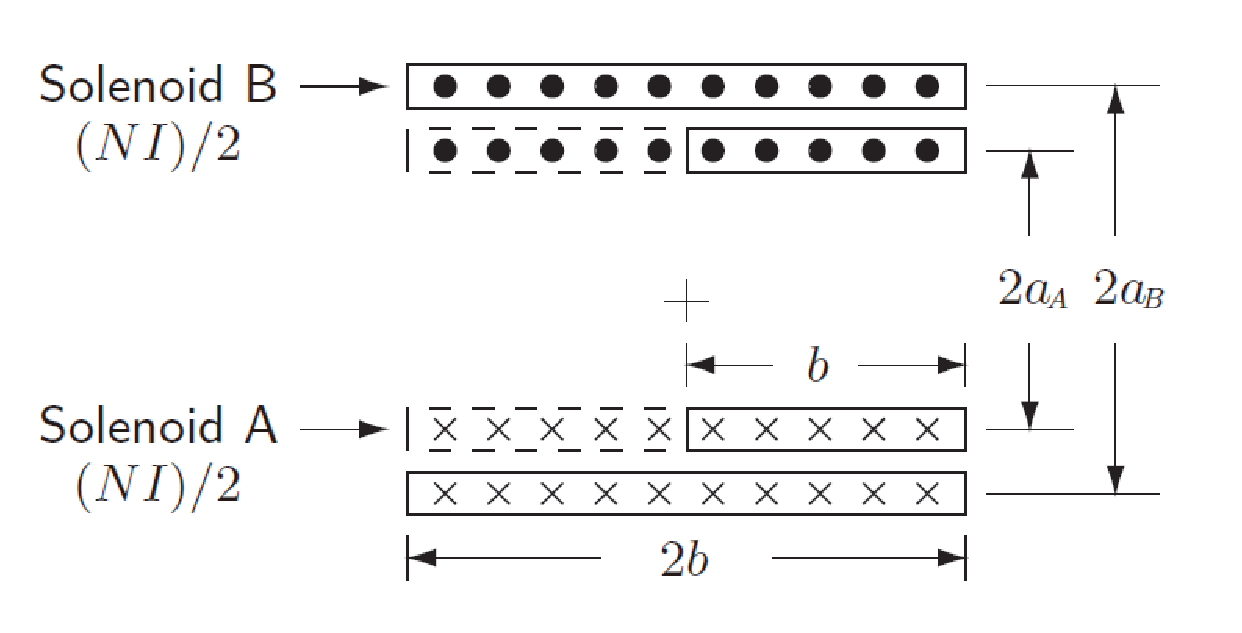
\includegraphics[scale=0.4]{chpt3/figs/fig3.8.eps}
  \caption{用以计算线圈A上的中心面轴向力的螺管线圈A和B的布局。}
\end{figure}

当一个螺管线圈不能被视为``薄壁''时,可以将之等效为径向上很多``薄壁''子线圈的组合。
这里,我们考虑对$\alpha>1$螺管线圈的最简单的处理方法:
将螺管分为两个``薄壁''子螺管A(内)和B(外),
两线圈长度均为$2b$,直径分别为$2a_A,2a_B$($2a_B >2a_A$),单位长度电流为$1/2(NI/2b)$。
一半子线圈A上的总轴向力$F_{zA}(0)$由两部分组成:
部分来自它自己的另一半,$F_{zAA}(0)$,可由3.41a给出;部分来自螺管线圈B,$F_{zAB}(0)$。
图3.8给出了两个子线圈的相对位置,基于这种结构我们推导螺管A的中平面上的轴向力。

比较图3.7和图3.8,我们发现式3.44经代换$2b_A = b; 2b_B = 2b; \rho = −2b$后可用于计算。
代入上述参数及式3.47给出的$c^2$,式3.44成为:
\begin{equation}
\begin{split}
F_{zAB}(0)=&-\frac{\mu_0}{2}(\frac{N_A I_A}{4b})\times \\
&\bigg(\frac{2b}{\sqrt{a_T^2+b^2}} \{[a_T^2+b^2][K(k_{b})-E(k_{b})]-\Upsilon(c^2,k_b)\}\\
&-\frac{2b}{\sqrt{a_T^2+4b^2}} \{[a_T^2+4b^2][K(k_{2b})-E(k_{2b})]-\Upsilon(c^2,k_{2b}) \}\bigg)
\end{split}
\end{equation}
式中,$a_T=a_A+a_B$。模量为:
$$k_{b}^2=\frac{4a_A a_B}{a_T^2+b^2} ;\qquad k_{2b}^2=\frac{4a_A a_B}{a_T^2+4b^2} $$

子螺管A施加在自身的中平面轴向力$F_{zAA}(0)$,可在式3.41a中用$NI/4b$代替$NI/2b$得到。
类似的,子螺管B受到的总中平面力$F_{zB}(0)$由$F_{zBB}(0)$和$F_{zBA}(0)$组成:
\begin{subequations}
	\begin{align}
F_{zA}(0) =& F_{zAA}(0)+F_{zAB}(0) \\
F_{zB}(0) =& F_{zBB}(0)+F_{zBA}(0)
	\end{align}
\end{subequations}

于是,
\begin{align}
F_{zA}(0)=&-\frac{\mu_0}{2}\left(\frac{N I}{4b}\right)\times \\\notag
&\bigg( \{2b\sqrt{4a_A^2+b^2}[K(k_{b_A})-E(k_{b_A})]-2b\sqrt{4a_A^2+4b^2}[K(k_{2b_A})-E(k_{2b_A})]\}\\\notag
&+\frac{2b}{\sqrt{a_T^2+b^2}} \{[a_T^2+b^2][K(k_{b})-E(k_{b})]-\Upsilon(c^2,k_b)\}\\\notag
&-\frac{2b}{\sqrt{a_T^2+4b^2}} \{[a_T^2+4b^2][K(k_{2b})-E(k_{2b})]-\Upsilon(c^2,k_{2b}) \}\bigg)
\end{align}

其中,$c^2$已在3.47给出。四个模量分别为:
$$k_{b_A}^2=\frac{4a_A^2}{4a_A^2+b^2} ;\quad k_{2b_A}^2=\frac{4a^2_A}{4a_A^2+4b^2};\quad
k_{b_B}^2=\frac{4a_B^2}{4a_B^2+b^2} ;\quad k_{2b_B}^2=\frac{4a^2_B}{4a_B^2+4b^2} $$

本例中,由于$2b_A=2b_B=2b$,$N_A I_A=N_B I_B$以及$F_{zAB}(0)=F_{zBA}(0)$。从而有:
\begin{equation*}
\begin{split}
F_{zB}(0)=&-\frac{\mu_0}{2}\left(\frac{N I}{4b}\right)\times \\
&\bigg( \{2b\sqrt{4a_B^2+b^2}[K(k_{b_B})-E(k_{b_B})]-2b\sqrt{4a_B^2+4b^2}[K(k_{2b_B})-E(k_{2b_B})]\}\\
&+\frac{2b}{\sqrt{a_T^2+b^2}} \{[a_T^2+b^2][K(k_{b})-E(k_{b})]-\Upsilon(c^2,k_b)\}\\
&-\frac{2b}{\sqrt{a_T^2+4b^2}} \{[a_T^2+4b^2][K(k_{2b})-E(k_{2b})]-\Upsilon(c^2,k_{2b}) \}\bigg)
\end{split}\tag{3.53b}
\end{equation*}

分为两个``薄壁''线圈的螺管受到的总中平面轴向力$F_{zT}(0)$为$F_{zA}(0)$和$F_{zB}(0)$之和。
于是得到:
\begin{equation}
\begin{split}
F_{zT}(0)=&-\frac{\mu_0}{2}\left(\frac{N I}{4b}\right)\times \\
&\bigg(2b\sqrt{4a_A^2+b^2}[K(k_{b_A})-E(k_{b_A})]-2b\sqrt{4a_A^2+4b^2}[K(k_{2b_A})-E(k_{2b_A})]\\
&+2b\sqrt{4a_B^2+b^2}[K(k_{b_B})-E(k_{b_B})]-2b\sqrt{4a_B^2+4b^2}[K(k_{2b_B})-E(k_{2b_B})]\\
&+\frac{4b}{\sqrt{a_T^2+b^2}} \{[a_T^2+b^2][K(k_{b})-E(k_{b})]-\Upsilon(c^2,k_b)\}\\
&-\frac{4b}{\sqrt{a_T^2+4b^2}} \{[a_T^2+4b^2][K(k_{2b})-E(k_{2b})]-\Upsilon(c^2,k_{2b}) \}\bigg)
\end{split}
\end{equation}

当一个螺管线圈被分为2个``薄壁''子螺管时,为获得$F_{zT}(0)$,要计算方程3.54中的4项;
当一个螺管线圈被分为$m>2$个``薄壁''子螺管时,则要计算$2(m!)/[(m−2)!]$项。
比如,$m=3$时,$F_{zT}(0)$的表达式中有12项,有18个模量,手算显然十分繁琐。

为了编写可用来精确计算``实际"螺管线圈(``厚壁")中平面轴向力的计算机程序,
我们必须按照$m$个``薄壁''线圈展开式3.54。
为了确保每一个子线圈是``薄壁''的,$m$可能是10或者更大。

多数情况下$c^2$是接近于1的,甚至对``长"螺管($\beta\gg 1$)也不可能近似$\Upsilon(c^2,k)$中的$\prod(c^2,k)$项。

\subsubsection{特例9:``长''的厚壁螺管的中平面力}
因为在大多数应用中有$c^2\simeq 1$,
式3.54中$\Upsilon(c^2,k)$项里的$\prod{(c^2,k)}$项不能由其级数展开的前几项近似。
不过,式3.54中的剩余项可以在$\beta \gg 1$时展开,正如特例5中所作的那样。于是:
\begin{align}
F_{zT}(0)\simeq& -\mu_0 \left(\frac{N I}{4b}\right)^2\left\{ \pi(a_A^2+a_B^2)-(a_A^2-a_B^2)^2\big[2\prod(c^2,k_b)-\prod(c^2,k_{2b})\big]\right\}  \\\notag
\simeq& -\mu_0 \left(\frac{N I}{4b}\right)^2 \pi(a_A^2+a_B^2) \left\{1-\frac{(a_A^2-a_B^2)^2}{\pi(a_A^2+a_B^2)}\big[2\prod(c^2,k_b)-\prod(c^2,k_{2b})\big]\right\}
\end{align}

当$a_A=a_B$时,式3.55约化为3.41b。
在式3.55的第二行中,大括号内的后一项可视为修正项。

\subsection{双线圈嵌套磁体的轴向力}
在一个由多个同轴对齐的嵌套螺管组成的磁体中,
有时计算各个螺管的中平面轴向压缩力非常重要;对大型的嵌套螺管磁体,如MRI磁体,则尤其重要。
这里我们考虑仅有两个薄壁螺管A和B组成的最简单的嵌套磁体,如图3.9。
螺线管A(内)的参数为$2a_A,2b_A,N_A I_A/2b_A$;
螺线管B(外)的参数为$2a_B, 2b_B, N_B I_B/2b_B$。

\begin{figure}[htbp]
  \centering
 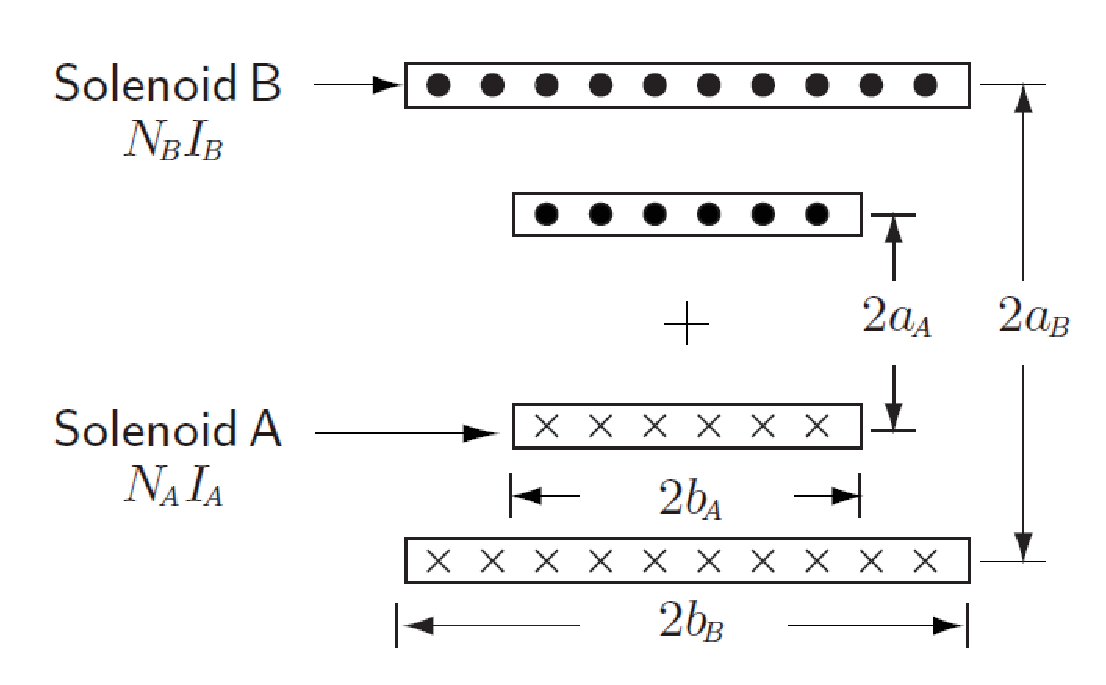
\includegraphics[scale=0.4]{chpt3/figs/fig3.9.eps}
  \caption{由螺管A和B组成的嵌套磁体}
\end{figure}

\subsubsection{螺管A所受中平面轴向力}

施于螺线管A右半部分的总中平面轴向力$F_{zA}(0)$是$F_{zAA}(0)$和$F_{zAB}(0)$之和。
其中,$F_{zAA}(0)$来自其自身左半部分,$F_{zAB}(0)$来自螺管B。
$F_{zAA}(0)$可在式3.41a中替换下标A给出。$F_{zAB}(0)$可由式3.44采取如下替代给出:
$b_A$替$2b_A$,$−(b_A+b_B)$替$\rho$,$2b_B$不变,$c^2$仍由式3.47给出。
\begin{align}
F_{zA}(0)=\frac{\mu_0}{2}\bigg[&\left(\frac{N_A I_A}{2b_A}\right)^2\times \{2b_A\sqrt{4a_A^2+b_A^2}[K(k_{bA})-E(k_{bA})]-2b_A\sqrt{4a_A^2+4b_A^2}[K(k_{2bA})-E(k_{2bA})]\}\\\notag
&+\left(\frac{N_AI_A}{2b_A}\right)\left(\frac{N_BI_B}{2b_B}\right)\bigg(\frac{2b_B}{\sqrt{a_T^2+b_B^2}}\{[a_T^2+b_B^2][K(k_B)-E(k_{B})]-\Upsilon(c^2,k_B)\}\\\notag
&-\frac{b_D}{\sqrt{a_T^2+b_D^2}}\{{[a_T^2+b_D^2][K(k_D)-E(k_D)]-\Upsilon(c^2,k_D)}\}\\\notag
&-\frac{b_T}{\sqrt{a_T^2+b_T^2}}\{[a_T^2+b_T^2][K(k_T)-E(k_T)]-\Upsilon(c^2,k_T^2)\}\bigg)\bigg]
\end{align}

其中,$a_T=a_A+a_B$,$b_D=b_B-b_A$以及$b_T=b_A+b_B$。模量$k_{b_A}, k_{2b_A}, k_A,k_B, k_{AB}$分别为:
$$ k_{bA}^2=\frac{4a_A^2}{4a_A^2+b_A^2}; k_{2bA}^2=\frac{4a_A^2}{4a_A^2+4b_A^2}; k_B^2=\frac{4a_Aa_B}{a_T^2+b_B^2};k_D^2=\frac{4a_Aa_B}{a_T^2+b_D^2}; k_T^2=\frac{4a_Aa_b}{a_T^2+b_T^2}$$


\subsubsection{特例10:螺管A所受中平面轴向力---``长''螺管}
当两个螺线管都是``长"($b_A^2\gg 4a_A^2;b_B^2\gg a_T^2$)的,但长度不一样,比如$b_D^2\gg a_T^2$。
式3.56可简化为:
\begin{align}
F_{zA}(0)\simeq -\frac{\mu_0}{2}\bigg\{&\left(\frac{N_AI_A}{2b_A}\right)^2\pi a_A^2+\left(\frac{N_AI_A}{2b_A}\right)\left(\frac{N_BI_B}{2b_{B}}\right)\times\\\notag
&(a_A-a_B)^2\big[\prod(c^2,k_D)+\prod(c^2,k_T)-2\prod(c^2,k_B)\big]\bigg\}
\end{align}

式3.57右侧的第二项代表$F_{zAB}$。
物理上,这是由螺管B的在螺管A的近螺管B端轴向位置上的磁场径向分量$B_r$引起的。
当$b_A\rightarrow \infty$和$b_B\rightarrow \infty$时,第二项趋于0。

\subsubsection{特例11:螺管A所受中平面轴向力---A和B均``长"但B比A更长}
当两个螺线管都如特例10中一样是``长"的但B远比A更长,
即$b_D\rightarrow b_B$以及$b_T\rightarrow b_B$。式3.57a可进一步化简为:
\begin{equation*}
F_{zA}(0)\simeq F_{zAA}(0)\simeq -\frac{\mu_0}{2}\left(\frac{N_AI_A}{2b_A}\right)^2\pi a_A^2 \tag{3.57b}
\end{equation*}

当$b_A/b_B\rightarrow 0$时有$F_{zAB}(0)\rightarrow 0$。这在物理上很容易理解,
因为螺管B比螺管A更长。式3.57右侧第二项给出的作为$F_{zAB}(0)$关键项的螺管B的$B_r$在其室温孔内是0,
而螺管A恰置于此处。

\subsubsection{螺管B所受中平面轴向力}
螺线管B的中平面轴向力表达式与螺管A非常相似。
我们可以通过变量替换的方式,直接由前几部分已给出的表达式得到。
螺管B所受总中平面轴向力$F_{zB}(0)$是$F_{zBB}(0)$与$F_{zBA}(0)$之和。
其中,$F_{zBB}(0)$来自其自身左半部分,$F_{zBA}(0)$来自螺管A。
\begin{align}
F_{zB}(0)=&-\frac{\mu_0}{2}\bigg[\left(\frac{N_BI_B}{2b_B}\right)^2\times\\\notag
&\left\{2b_B\sqrt{4a_B^2+b_B^2}[K(k_{bB})-E(k_{bB})]-2b_B\sqrt{4a_B^2+4b_B^2}[K(K_{2bB})-E(k_{2bB})]\right\}\\\notag
&+\left(\frac{N_BI_B}{2b_B}\right)\left(\frac{N_AI_A}{2b_A}\right)\bigg(\frac{2b_A}{\sqrt{a_T^2+b_A^2}}\{[a_T^2+b_A^2][K(k_A)-E(k_A)]-\Upsilon(c^2,k_A)\}\\\notag
&+\frac{b_D}{\sqrt{a_T^2+b_D^2}}\{[a_T^2+b_D^2][K(k_D)-E(k_D)]-\Upsilon(c^2,k_D)\}\\\notag
&-\frac{b_T}{\sqrt{a_T^2+b_T^2}}\{[a_T^2+b_T^2][K(k_T)-E(k_T)]-\Upsilon(c^2,k_T)\}\bigg)\bigg]
\end{align}

式中的$c^2$同样由式3.47给出。模量$k_{2b_B},k_A$如下式,其他模量与式3.56相同:
\begin{equation*}
k_{2bB}^2=\frac{a_B^2}{4a_B^2+4b_B^2};\quad \quad k_A^2=\frac{4a_Aa_B}{a_T^2+b_A^2}
\end{equation*}

\subsubsection{特例12:螺管B所受中平面轴向力---A和B均``长"但B比A更长}
条件参数与特例11所述相同,我们有:
\begin{align}
F_{zB}(0)\simeq -\frac{\mu_0}{2}\bigg\{&\left(\frac{N_BI_B}{2b_B}\right)^2\pi a_B^2+\left(\frac {N_BI_B}{2b_B}\right)\left(\frac{N_AI_A}{2b_A}\right)\bigg[\pi(a_A^2+a_B^2)\\\notag
&-(a_A-a_B)^2\big[2\prod(c^2,k_A)+\prod(c^2,k_D)-\prod(c^2,k_T)\big]\bigg]\bigg\}
\end{align}

与特例11类似,式3.59中第二项表示的$F_{zBA}$不可忽略,
因为螺管A的$B_r$在螺管B靠近螺管A两端的轴向位置上均不可忽略。

\subsubsection{特例13:螺管B所受中平面轴向力---A和B均``长"但B比A短很多}
当两个螺管都是``长"的($b_B^2\gg a_T^2;b_A^2\gg a_T^2$)但螺管B比螺管A短很多
($b_D^2\rightarrow b_A^2\gg a_T^2$)时,式3.58简化为:
\begin{equation*}
F_{zB}(0)\simeq-\frac{\mu_0}{2}\left(\frac{N_BI_B}{2b_B}\right)^2\pi a_B^2 \tag{3.59b}
\end{equation*}

式3.59可类比于特例11中的式3.57b;那里的物理解释也可以用在这里。


\subsection{轴向偏心螺管组的轴向恢复力}
当螺管A和螺管B的轴向场指向同一方向但中轴线失配距离为$\rho$时,
会产生一个轴向恢复力$F_{zR}(\rho)$,让两者中轴线对齐。$F_{zR}(\rho)$可写为:
\begin{align}
F_{zR}(\rho)=&-\frac{\mu_0}{2}\left(\frac{N_AI_A}{2b_A}\right)\left(\frac{N_BI_B}{2b_B}\right)\times\\\notag
&\bigg(\frac{b_T-\rho}{\sqrt{a_T^2+(b_T-\rho)^2}}\left\{[a_T^2+(b_T-\rho)^2][K(k_{T-})-E(k_{T-})]-\Upsilon(c^2,k_{T-})\right\}\\\notag
&+\frac{b_D+\rho}{\sqrt{a_T^2+(b_T+\rho)^2}}\left\{[a_T^2+(b_D+\rho)^2][K(k_{D+})-E(k_{D+})]-\Upsilon(c^2,k_{D+})\right\}\\\notag
&-\frac{b_T+\rho}{\sqrt{a_T^2+(b_T+\rho)^2}}\left\{[a_T^2+(b_T+\rho)^2][K(k_{T+})-E(k_{T+})]-\Upsilon(c^2,k_{T+})\right\}\\\notag
&-\frac{b_D-\rho}{\sqrt{a_T^2+(b_D-\rho)^2}}\left\{[a_T^2+(b_D-\rho)^2][K(k_{D-})-E(k_{D-})]-\Upsilon(c^2,k_{D-})\right\}\bigg)
\end{align}
式中,$a_T=a_A+a_B, b_T=b_A+b_B, b_D=b_A−b_B$。模量为:
$$
k_{T+}^2=\frac{4a_Aa_B}{a_T^2+(b_T+\rho)^2};\qquad k_{T-}^2=\frac{4a_Aa_B}{a_T^2+(b_T-\rho)^2};$$
$$k_{D+}^2=\frac{4a_Aa_B}{a_T^2+(b_D+\rho)^2}; \qquad k_{D-}^2=\frac{4a_Aa_B}{a_T^2+(b_D-\rho)^2}$$


\subsubsection{特例14:轴向对齐}
当$\rho=0, k_{T+}^2=k_{T-}^2, k_{D+}^2=k_{D-}^2$时,有$F_{zR}(\rho)=0$。这和物理上的预期一致。

\subsubsection{特例15:``小''的轴向失配}
对于很小的失配,规定为$\rho\ll \sqrt{a_T^2+b_D^2}$,$F_{zR}(\rho)$正比于$\rho$:
\begin{equation}
F_{zR}(\rho)\propto-\left(\frac{N_AI_A}{2b_A}\right)\left(\frac{N_BI_B}{2b_B}\right)\rho
\end{equation}

后文将使用式3.61推导小轴向失配($\rho\ll \sqrt{a_T^2+b_D^2}$)螺管A和B间的互感$M_{AB}(\rho)$。

\subsubsection{特例16:螺管之一是``长"的}
如果螺管A或螺管B之一是``长"的,那个更长的螺管的轴向场将成为均匀的,其$B_r$就很小了。
哪怕两个线圈之间存在较大的失配,长螺管对短螺管只有很小的轴向力。
在$b^2_T\gg a_T^2,b_D^2\gg a_T^2$时,式3.60中前两个$+$项和后两个$-$项抵消,结果有$F_{zR}(\rho)\rightarrow 0$。

\section{螺管在磁力下的应力应变}
本节我们研究螺管磁体中的超导体(主要是)在洛伦兹力下的应力和应变[3.6]。
这里推导出来的磁应力解析解和图像都是在``简单''场分布下的应用绕组材料的``简化''性质条件下得到的。

\subsection{应力应变方程}
轴向磁场$B_z(r,z)$对电流$\lambda J$作用而产生的磁场力在螺管绕组中引起的应力
(径向$\sigma_r(r,z)$,周向$\sigma_\theta(r,z)$,轴向$\sigma_z(r,z)$,剪切$\tau_{rz}(r,z)$)可通过解以下平衡方程得到:
\begin{subequations}
	\begin{align}
\frac{\partial\sigma_{r}}{\partial_r}+\frac{\sigma_{r}-\sigma_{\theta}}{r}+\frac{\partial \tau_{rz}}{\partial z}=&-\lambda JB_z(r,z)\\
\frac{\partial \tau_{rz}}{\partial r}-\frac{\tau_{rz}}{r}+\frac{\partial \sigma_z}{\partial z}=&-\lambda JB_r(r,z)
	\end{align}
\end{subequations}

相应的边界条件为:$\sigma_r(r=a_1,z)=0;\sigma_r(r=a_2,z)=0;\sigma_z(r,z=\pm b)=0;\tau_{rz}(r=a_1,z)=0;\tau_{rz}(r=a_2,z)=0;\tau_{rz}(r,z=\pm b)=0$。
可见,剪切力是耦合式3.62a和3.62b的唯一变量。大多数LTS和HTS复合超导体都可以视为正交各向异性,
即可用Hooke定律。正交各向异性材料的Young模量,Poisson比等机械性质在三个正交方向不同但关于正交方向对称。
应变$\epsilon_r,\epsilon_\theta,\epsilon_z$分别为$r,\theta,z$向,剪切应变$\gamma_{rz}$位于$r-z$平面,各自与相应应力关联:
\begin{subequations}
	\begin{align}
\epsilon_r=&\frac{1}{E_r}\sigma_r-\frac{\nu_{\theta r}}{E_{\theta}}\sigma_{\theta}-\frac{\nu_{zr}}{E_z}\sigma_z+\epsilon_{T_r}\\
\epsilon_\theta=&-\frac{\nu_{r\theta}}{E_r}\sigma_r+\frac{1}{E_{\theta}}\sigma_{\theta}-\frac{\nu_{z\theta}}{E_z}\sigma_z+\epsilon_{T_\theta}\\
\epsilon_z=&-\frac{\nu_{rz}}{E_r}\sigma_r-\frac{\nu_{\theta z}}{E_{\theta}}\sigma_{\theta}+\frac{1}{E_z}\sigma_z+\epsilon_{T_z}\\
\gamma_{rz}=&\frac{1}{G_{{rz}}}\tau_{rz}
	\end{align}
\end{subequations}
式中,$E_r, E_\theta, E_z$分别是$r,\theta,z$向的杨氏模量。
$\nu_{12}\equiv -\epsilon_2/\epsilon_1$是当材料应力加在1方向时($\sigma_1;\sigma_2=\sigma_3=0$)两个正交方向的横向应变的Poisson比。$G_{rz}$是剪切模量。 
$\epsilon_{T_r},\epsilon_{T_\theta},\epsilon_{T_z}$分别为从室温$300\ \mathrm{K}$到运行温度$T_{op}$的热膨胀积分系数。
\begin{equation*}
\epsilon_{T_r}=\int_{300\ \mathrm{K}}^{T_{op}}\alpha_{Tr}(T)dT;\quad
\epsilon_{T_\theta}=\int_{300\ \mathrm{K}}^{T_{op}}\alpha_{T_\theta}(T)dT;\quad
\epsilon_{T_z}=\int_{300\ \mathrm{K}}^{T_{op}}\alpha_{Tz}(T)dT \tag{3.63e}
\end{equation*}
式中,$\alpha_{T_r}(T),\alpha_{T_\theta}(T),\alpha_{T_z}(T)$分别为平行于主轴的依赖于温度的热膨胀系数。
因为这些系数为正且从$300\ \mathrm{K}$到度$T_{op}<300\ \mathrm{K}$积分,
可知式3.63a-3.63c中的热应变为负,即压缩。

同时应用下列$\nu$和$E$关系:
\begin{equation*}
\frac{\nu_{r\theta}}{E_\theta}=\frac{\nu_{\theta r}}{E_r};\quad \frac{\nu_{\theta z}}{E_z}=\frac{\nu_{z\theta}}{E_\theta};\quad \frac{\nu_{zr}}{E_r}=\frac{\nu_{rz}}{E_z} \tag{3.63f}
\end{equation*}

对于轴对称体,例如理想螺线管,在$r$和$z$方向的应变$u_r$和位移$u_z$关系为:
\begin{equation*}
\epsilon_r=\frac{\partial {u_r}}{\partial r};\quad \epsilon_\theta=\frac{u_r}{r};\quad \epsilon_z=\frac{\partial {u_z}}{\partial z};\quad \gamma_{rz}=\frac{\partial {u_r}}{\partial z}+\frac{\partial {u_z}}{\partial r} \tag{3.63g}
\end{equation*}

由于轴对称,式3.62中的所有变量都与$\theta$无关,且有$u_\theta=0$。
一般的,不同时存在$\sigma_r$(3.62a)和$\sigma_z$(3.62b)的闭式解。
对``长"螺管,例如多用于空间高均匀磁场NMR磁体中的螺管,
其$B_z(r,z)$在$z$方向至少是在以中平面为起点的很长范围内的变化都很小。
剪切应力$\tau_{rz}$是由$B_z(r,z)$在线圈上产生的径向载荷的变化导致的。
因此,在一个长螺管中,我们可假设所有变量都不依赖于$z$(包括$u_r$,即$\partial u_r/\partial z=0$),
以化简式3.62a。因为在高均匀磁场磁体中有$\partial B_r(r,z)/\partial z\simeq 0$,
故可以放心的假设在磁体轴向的大部分长度上有$\partial u_r/\partial z=0$成立。
加上$\partial u_z/\partial r=0$,结果有$\gamma_{rz}=\tau_{rz}=0$。
反过来,这个结果会解耦式3.62a和3.62b。

联立式3.62和3.63,假设$\tau_{rz}=0$,用$u_r$解出$\sigma_r$和$\sigma_{\theta}$,我们得到以下微分方程:
\begin{subequations}
	\begin{align}
&\frac{d^2u_r}{d_r^2}+\frac{1}{r}\frac{du_r}{dr}-\zeta^2\frac{u_r}{r^2}=-\frac{1-\nu_{r\theta}\nu_{\theta r}}{E_r}\lambda JB_z(r)+\frac{F}{r}\\
&\mbox{其中,\quad}\zeta=\sqrt{\frac{E_\theta}{E_r}};\quad F=
-(\zeta^2-\nu_{r \theta})\epsilon_{T_\theta}+(1-\nu_{\theta r}\zeta^2)\epsilon_{Tr}
	\end{align}
\end{subequations}

式3.64a的通解为:
\begin{equation}
u_r=C_1r^\zeta+\frac{C_2}{r^\zeta}+u_r^L+u_r^T
\end{equation}
式中,$C_1,C_2$是由$r = a_1, r = a_2$边界条件确定的常数。
$u^L_r$和$u^T_r$ (上标$L$和$T$分别代表Lorentz和Thermal)为依赖于式3.64a等式右侧``源''项的特解。
热学项$u^T_r$为:
\begin{equation}
u_r^T=\frac{Fr}{1-\zeta^2}
\end{equation}

对各向同性材料($E_\theta =E_r,\zeta =1$),$u_r^T$为:
\begin{equation}
u_r^T(\zeta=1)=\frac{1}{2}Fr \ln r
\end{equation}

一般的,$B_z(r)$可以用幂级数给出:
\begin{equation}
B_z(r)=\sum_{k=0}^{n}b_kr^k
\end{equation}

于是,Lorentz项可以表示为:
\begin{equation}
u_r^T=\frac{1-\nu_{r\theta}\nu_{\theta r}}{E_r}\lambda J\sum_{k=0}^{n}\frac{b_k r^{k+2}}{\zeta^2-(k+2)^2}
\end{equation}

\subsection{各向同性螺管的应力应变方程}
本节我们推导绕组电流密度为$\lambda J$的各向同性螺管的径向和周向的应力。
绕组中的轴向场随$r$线性变化,变化范围为$B_z(r = a_1)\equiv B_1$到$B_z(r = a_2)\equiv B_2$。
注意到在嵌套线圈磁体中,$B_1,B_2$中都可能含有由位于外部的``长"线圈产生的均匀背景场。
定义两个无量纲参数:$\kappa\equiv B_2/B_1,\rho = r/a_1$。
在高场NMR磁体中,最内部的线圈的$\kappa$会超过$0.9$;
对孤立线圈,$\kappa$大概是$-0.1$;对于无限长孤立线圈,有$\kappa=0$。
于是,式3.62a可以重写为:
\begin{equation}
\frac{d\sigma_{\rho}}{d\rho}+\frac{\sigma_\rho-\sigma_\theta}{\rho}=-\frac{\lambda JB_1a_1}{\alpha-1}[\alpha-\kappa-(1-\kappa)\rho]
\end{equation}

对于各向同性材料,考虑热应变$\epsilon_T$后的总应变为:
\begin{subequations}
	\begin{align}
\epsilon_\rho=&\frac{1}{E}(\sigma_\rho-\nu\sigma_\theta)+\epsilon_T\\
\epsilon_\theta=&\frac{1}{E}(\sigma_\theta-\nu\sigma_\rho)+\epsilon_T
	\end{align}
\end{subequations}

从上式中解出$\sigma_\rho,\sigma_{\theta}$:
\begin{subequations}
	\begin{align}
\sigma_\rho=&\frac{E}{1-\nu^2}[\epsilon_\rho+\nu\epsilon_\theta-(1+\nu)\epsilon_T]\\
\sigma_\theta=&\frac{E}{1-\nu^2}[\epsilon_\theta+\nu\epsilon_\rho-(1+\nu)\epsilon_T]
	\end{align}
\end{subequations}

应变和位移$u$有关(此处仅考虑$r$向):
\begin{equation*}
\epsilon_\rho=\frac{1}{a_1}\frac{du}{d\rho};\quad \epsilon_\theta=\frac{1}{a_1}\frac{u}{\rho} \tag{3.72c}
\end{equation*}

联立式3.72a-3.72c,得:
\begin{align*}
\sigma_\rho=&\frac{E}{(1-\nu^2)a_1}\left[\frac{du}{d\rho}+\nu\frac{u}{\rho}-a_1(1+\nu)\epsilon_T\right]\tag{3.72d}\\ 
\sigma_\theta=&\frac{E}{(1-\nu^2)a_1}\left[\frac{u}{\rho}+\nu\frac{du}{d\rho}-a_1(1+\nu)\epsilon_T\right] \tag{3.72e}
\end{align*}

联立式3.70和3.92d,3.72e,得到:
\begin{equation}
\frac{d^2u}{d\rho^2}+\frac{1}{\rho}\frac{du}{d\rho}-\frac{u}{\rho^2}=-\left(\frac{1-\nu^2}{E}\right)\left(\frac{\lambda JB_1a_1^2}{\alpha-1}\right)[\alpha-\kappa-(1-\kappa)\rho] %(3.73)
\end{equation}

方程3.73的通解为:
\begin{equation}
u=C_1\rho+\frac{C_2}{\rho}-\left(\frac{1-\nu^2}{E}\right)\left(\frac{\lambda JB_1a_1^2}{\alpha-1}\right)\left[\frac{(\alpha-\kappa)\rho^2}{3}-\frac{(1-\kappa)\rho^3}{8}\right]%\(3.74)
\end{equation}
式中,$C_1,C_2$是由$\rho=1$和$\rho=\alpha$处的边界条件确定的常数;最后一项是特解。联立式3.74,3.72d和3.72e,得:
\begin{subequations}
	\begin{align}
\sigma_\rho=&\frac{E}{(1-\nu^2)a_1}\left[(1+\nu)C_1-(1-\nu)\frac{C_2}{\rho^2}\right] \\ \nonumber
&-\left\{\frac{\lambda JB_1a_1}{\alpha-1}\left[\frac{2+\nu}{3}(\alpha-\kappa)\rho-\frac{3+\nu}{8}(1-\kappa)\rho^2\right]\right\}-\frac{E\epsilon_T}{1-\nu}\\
\sigma_\theta=&\frac{E}{(1-\nu^2)a_1}\left[(1+\nu)C_1+(1-\nu)\frac{C_2}{\rho^2}\right]\\ \nonumber
&-\left\{\frac{\lambda JB_1\alpha_1}{\alpha-1}\left[\frac{1+2\nu}{3}(\alpha-\kappa)\rho-\frac{1+3\nu}{8}(1-\kappa)\rho^2\right]\right\}-\frac{E\epsilon_T}{1-\nu}
	\end{align}
\end{subequations}

代入$\sigma_{\rho}(1)=0$和$\sigma_{\rho}(\alpha)=0$,我们得到$C_1,C_2$的表达式:
\begin{subequations}
	\begin{align}
{[(1+\nu)C_1-(1-\nu)C_2]}=&\frac{1-\nu^2}{E}\left(\frac{\lambda JB_1a_1^2}{\alpha-1}\right)
\times\left[\frac{2+\nu}{3}(\alpha-\kappa)-\frac{3+\nu}{8}(1-\kappa)\right]\notag\\
&+a_1(1+\nu)\epsilon_T\\
{[(1+\nu)C_1-(1-\nu)\frac{C_2}{\alpha^2}]}=&\frac{1-\nu^2}{E}\left(\frac{\lambda JB_1a_1^2}{\alpha-1}\right) \times\left[\frac{2+\nu}{3}(\alpha-\kappa)\alpha-\frac{3+\nu}{8}(1-\kappa)\alpha^2\right]\notag\\
& +a_1(1+\nu)\epsilon_T
	\end{align}
\end{subequations}

解出$C_1,C_2$:
\begin{align*}
C_1=&\frac{1-\nu}{E}\left(\frac{\lambda JB_1a_1^2}{\alpha^2-1}\right)
\times\left[\frac{2+\nu}{3}(\alpha-\kappa)(\alpha^2+\alpha+1)
-\frac{3+\nu}{8}(1-\kappa)(\alpha+1)(\alpha^2+1)\right] \notag\\
&+a_1\epsilon_T\tag{3.76c}\\
C_2=&\frac{1+\nu}{E}\left(\frac{\lambda JB_1a_1\alpha^2}{\alpha^2-1}\right)\times \left[\frac{2+\nu}{3}(\alpha-\kappa)-\frac{3+\nu}{8}(1-\kappa)(\alpha+1)\right]\tag{3.76d}
\end{align*}

将3.76c和3.76d代入3.75,可得:
\begin{subequations}
	\begin{align}
\sigma_\rho=\frac{\lambda JB_1a_1}{\alpha-1}&\bigg[\frac{2+\nu}{3}(\alpha-\kappa)\left(\frac{\alpha^2+\alpha+1-\frac{\alpha^2}{\rho^2}}{\alpha+1}-\rho\right) \\ \nonumber
&-\frac{3+\nu}{8}(1+\kappa)\left(\alpha^2+1-\frac{\alpha^2}{\rho^2}-\rho^2\right)\bigg]\\
\sigma_\theta=\frac{\lambda JB_1a_1}{\alpha-1}&\bigg\{(\alpha-\kappa)\big[\frac{2+\nu}{3}\left(\frac{\alpha^2+\alpha+1+{\frac{\alpha^2}{\rho^2}}}{\alpha+1}\right)-\frac{1+2\nu}{3}\rho\big] \\ \nonumber
&-(1-\kappa)\big[\frac{3+\nu}{8}\left(\alpha^2+1+\frac{\alpha^2}{\rho^2}\right)-\frac{1+3\nu}{8}\rho^2\big]\bigg\}
	\end{align}
\end{subequations}

\subsubsection{``薄壁''线圈}
图3.10a和3.10b分别画出了``薄壁''线圈(这里$\alpha=1.2$)的归一化周向应力$\varsigma_\theta$($\equiv \sigma_{\theta}/(\lambda J B_1 a_1)$)和径向应力$\varsigma_r$($\equiv \sigma_{\rho}/(\lambda J B_1 a_1)$)与归一化径向距离$\rho$($\equiv r/a_1$ )在几个特定的``磁场比"$\kappa$($equiv B_2/B_1$)下的关系。
应注意,$\kappa=-0.1$对应孤立螺管;$\kappa=0$对应无限长线圈;$\kappa>0$对应处于均匀背景场中的线圈。

对各个磁场比$\kappa$,$\varsigma_\theta$均为$\rho$的减函数。
而$\varsigma_r$不同,在$r=a_1$和$r=a_2$时为零,在绕组径向中间位置有极值(极大或极小)。

对于$\kappa>0.5$,绕组总体上有一个正的径向应力,倾向于将各匝分开。
这种情况一般是应当避免的。减小绕组应力$\varsigma_r$的正效应问题将在3.6.3中简要讨论。
\begin{figure}
  \centering
 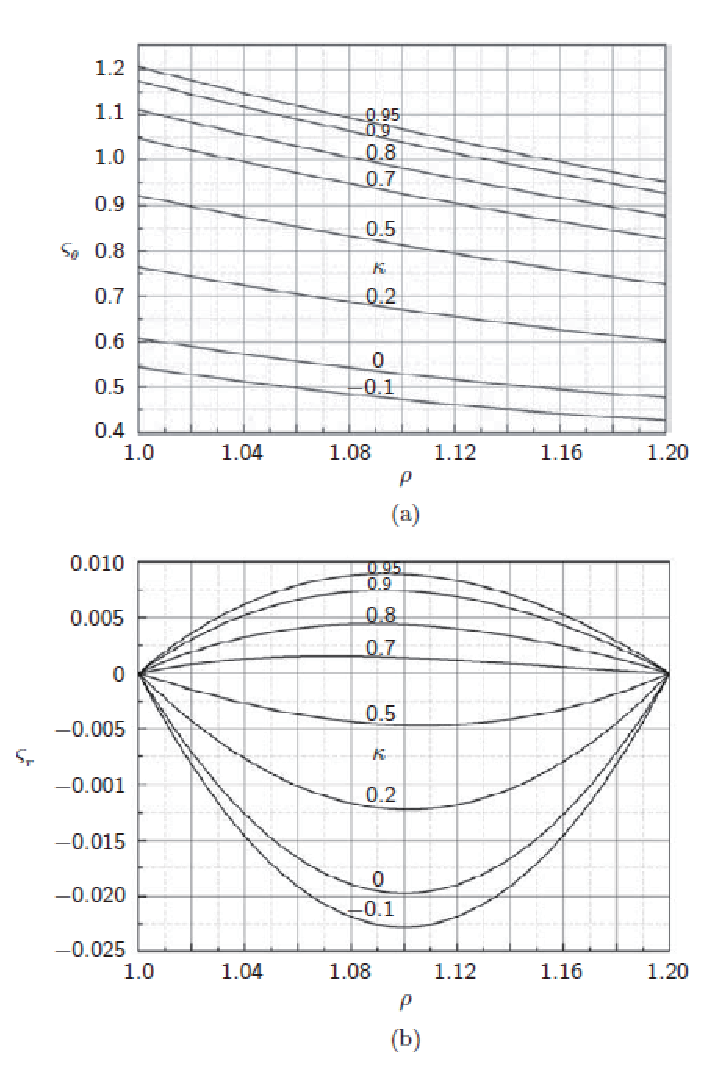
\includegraphics[scale=0.8]{chpt3/figs/fig3.10.eps}
  \caption{几个$\kappa\equiv B_2/B_1$值下的``薄壁''线圈($\alpha=1.2$)的特性图:a)归一化周向应力$\varsigma_\theta\equiv \sigma_\theta/(\lambda J B_1 a_1)$ vs. 归一化径向距离$\rho\equiv r/a_1$;
  b)归一化径向应力$\varsigma_r \equiv \sigma_\rho/(\lambda J B_1 a_1)$ vs. 归一化径向距离$\rho$。图中的$\kappa$的取值为$-0.1$(最下);$0$;$0.2$;$0.5$;$0.7$;$0.8$;$0.9$;$0.95$(最顶) }
\end{figure}

\subsubsection{``中等壁厚"线圈}
图3.11给出了``中等壁厚"线圈($\alpha=1.8$)的类似于图3.10的特性。
在这个``中等壁厚"线圈中,在$\kappa\simeq 0.2$时有$\varsigma>0$;
在$\kappa> 0.8$时$\varsigma$超过0.1。
也即,高背景场磁体室温孔中的``内插''线圈应当是``薄壁''的;不然,就要将之切分为多个``薄壁''的。

\begin{figure}
  \centering
 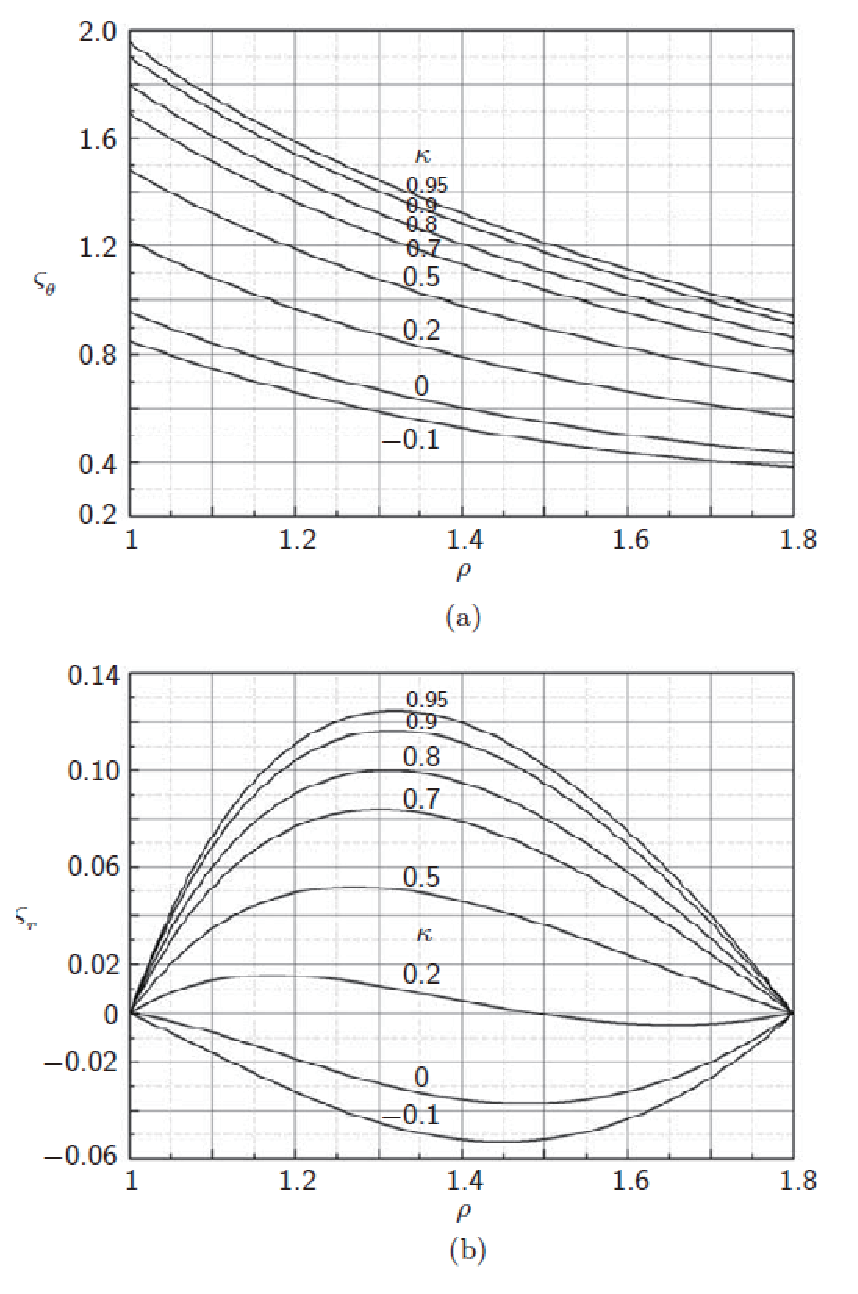
\includegraphics[scale=0.7]{chpt3/figs/fig3.11.eps}
  \caption{几个$\kappa\equiv B_2/B_1$值下的``中等壁厚"线圈($\alpha=1.8$)的特性图:(a)$\varsigma_\theta\equiv \sigma_\theta/(\lambda J B_1 a_1)$ vs.$\rho$;
  (b)$\varsigma_r \equiv \sigma_r/(\lambda J B_1 a_1)$ vs. $\rho$。各图中,$\kappa$的取值均为$-0.1$(最下);$0$;$0.2$;$0.5$;$0.7$;$0.8$;$0.9$;$0.95$(最顶) }
\end{figure}

\subsubsection{``厚壁''线圈}
图3.12给出了``厚壁''线圈($\alpha=3.6$)的特性图。
注意到此时$\varsigma_\theta$大致是``中等壁厚"线圈的2倍。
``厚壁线圈''最典型的特征是只在$\kappa$明显小于0时其归一化径向应力$\sigma_r$才大于零。

有两种实用方法可以令$\sigma_{r}$接近0或者成为负值:
1) 预应力绕制线圈;
2) 在最外层用具有高弹性模量的材料进行绑扎。
同时,将线圈分割为更薄的线圈不仅降低$\sigma_{r}$还降低$\sigma_{\theta}$。
\begin{figure}
  \centering
 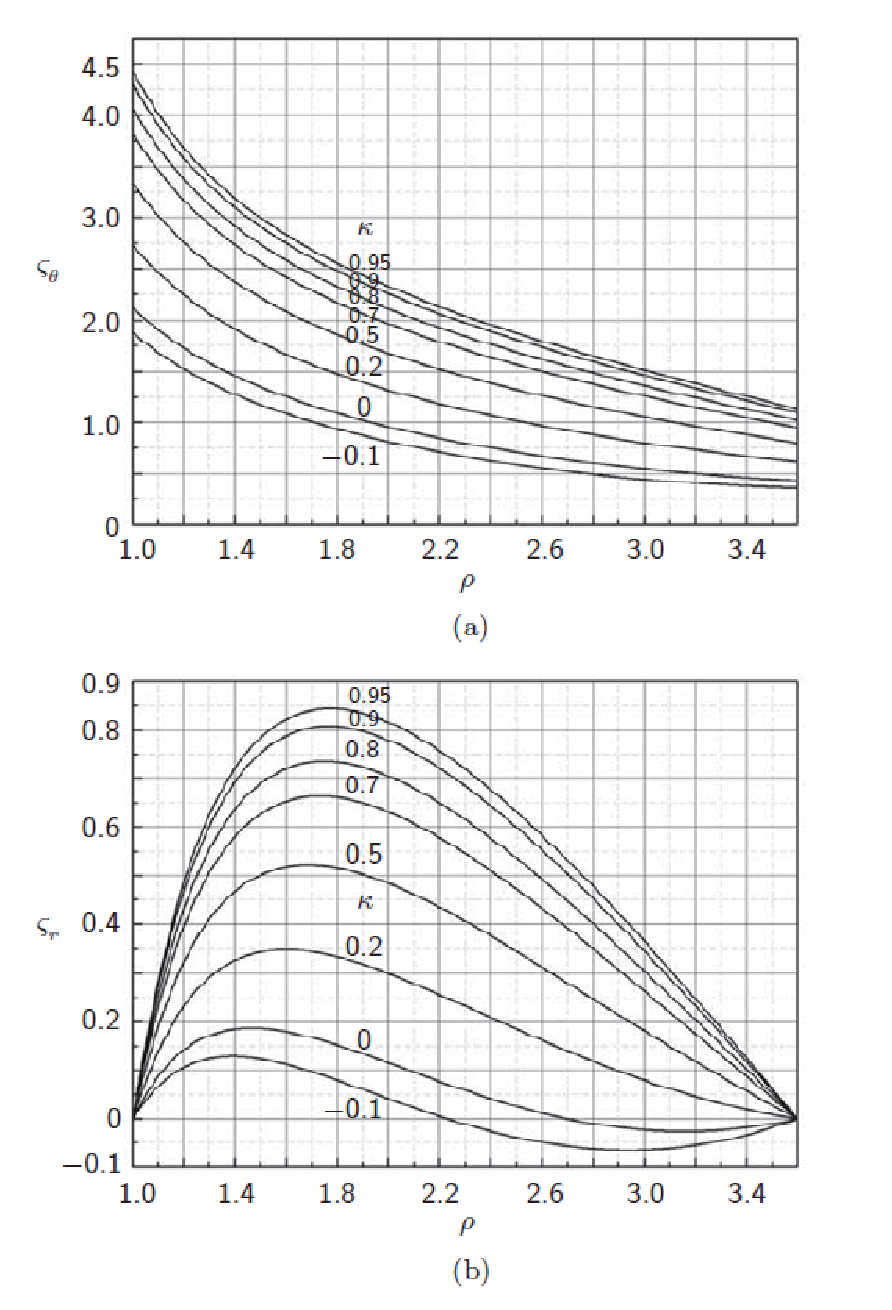
\includegraphics[scale=0.7]{chpt3/figs/fig3.12.eps}
  \caption{几个$\kappa\equiv B_2/B_1$值下的``厚壁''线圈($\alpha=3.6$)的特性图:
(a) $\varsigma_\theta\equiv \sigma_\theta/(\lambda J B_1 a_1)$ vs. $\rho$;
  (b) $\varsigma_r \equiv \sigma_r/(\lambda J B_1 a_1)$ vs. $\rho$。各图中,$\kappa$的取值均为$-0.1$(最下);$0$;$0.2$;$0.5$;$0.7$;$0.8$;$0.9$;$0.95$(最顶) }
\end{figure}

\subsection{张力绕制以减小径向应力}
这里用演示性的例子来说明张力绕制对减小径向应力$\sigma_{r}$的好处。
如前所述,$\sigma_{r}$在绕组中应为\textit{负}值以保证各层不会在径向崩析。
简单来说,当线圈是由预张力导体绕成时,张力产生向内的径向应力,从而减小了绕组内部的径向应力。
即使绕制过程张力维持恒定,张力效应在绕组中径向的分布也很难写为磁场体力的近似表达式。
由于绕组张力的存在,轴向和径向的应力只能通过数值分析计算得到。

考虑一个放置于高场背景磁体室温孔内的内插线圈。
内插线圈的参数为内径$2a_1=87\ \mathrm{mm}$,外径$2a_2=156.6\ \mathrm{mm}$,对应$\alpha = 1.8$:
这是一个``中等壁厚"磁体。分析中,假设线圈是``长"的。
其他参数包括:
$B_z(r=a_1)\equiv B_1 =28.1\ \mathrm{T}; B_z(r=a_2)\equiv B_2 =24.3\ \mathrm{T};\kappa\equiv B_2/B_1 = 0.865; \lambda J =8.26×10^7 \ \mathrm{A/m^2}$。
图3.11给出了$\alpha=1.8$时的$\varsigma_r(\rho)$曲线。
从图中,我们找到归一化径向应力$\varsigma_r\equiv \sigma_r/(\lambda J B_1 a_1)$的最大值为0.11,
在$\rho=r/a_1=1.3$时取得。于是,最大径向应力为:
\begin{align*}
  [\sigma_r]_{mx}=&0.11\lambda JB_1 a_1 \\
   =&0.11(8.26\times 10^7 \ \mathrm{A/m^2})(28.1\ \mathrm{T})(43.5\times 10^{-3}\ \mathrm{m})=11.1\ \mathrm{MPa}
\end{align*}

内插线圈难以承受大如$11.1\ \mathrm{MPa}$的径向应力。
图3.13给出了在从0到最大$200\ \mathrm{N}$($\simeq 20\ \mathrm{kg}$)范围内
几个绕制张力$\Gamma$下的$\sigma_{r}$和$r$的关系。
本图说明,绕制张力至少要$160\ \mathrm{N}$才能保证$\sigma_{r}$近似为0或为负值。
实践中,可能用到大至200 N的张力来绕线圈。
对于该内插线圈,绕制张力在$80\ \mathrm{N}$时,最大应力减小至大约$5\ \mathrm{MPa}$;
当线圈是用环氧浸渍时,正的径向$5\ \mathrm{MPa}$应力是可以承受的。
\begin{figure}[htbp]
  \centering
 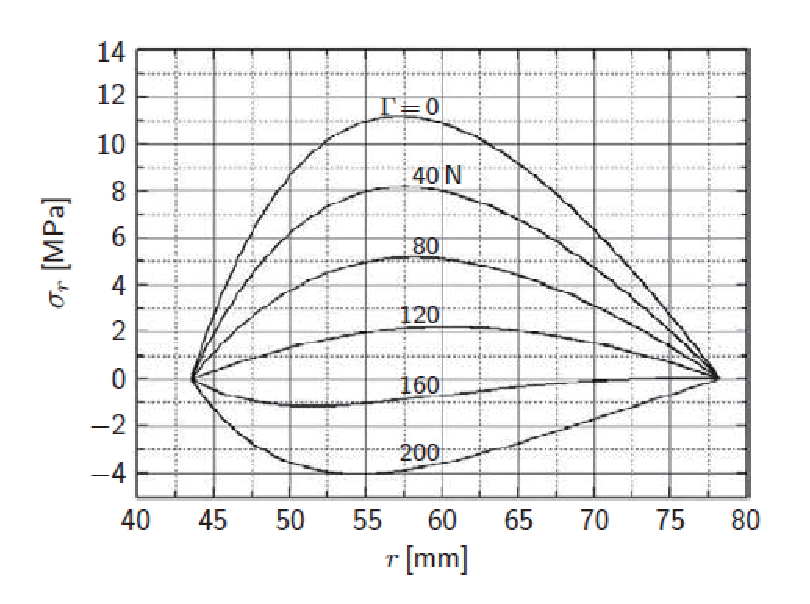
\includegraphics[scale=0.7]{chpt3/figs/fig3.13.eps}
  \caption{$\alpha=1.8$的螺管线圈在不同张力$\Gamma$下的$\sigma_r$ vs.$r$。$\Gamma=0$时,$\sigma$取得峰值,在$r\simeq 57.5\ \mathrm{mm}$处约为$11.1\ \mathrm{MPa}$。当张力大于$160\ \mathrm{N}$($\simeq 16\ \mathrm{kg}$)后,处处$\sigma_r\le 0 $。}
\end{figure}





\section{自感}
线圈的总磁链$\Phi$正比于通过线圈的电流$I$:
\begin{equation}
 \Phi=LI %page106
\end{equation}

比例系数$L$称为线圈自感。
我们注意到,$\Phi$是一个``场"概念量,而$I$是一个``路"概念量。
$L$将这两个概念连接起来。由于``场"概念必然涉及体积,故$L$是一个与几何有关的量。
此外,$L$还与线圈中存储的磁能$E_m$有关:
\begin{equation}
 E_m=\frac{1}{2}LI^2 %page106
\end{equation}

对于不含有磁性材料的系统,$E_m$可通过在整个空间积分$(1/2)\mu_0 H^2$得到。
可见,$E_m$也是一个``场"概念量;$L$通过式3.79将$E_m$和$I$联系在一起。

\subsection{圆形闭合回路的自感}
Maxwell推导了半径为$a$、磁导率为$\mu$的导线围成的半径为$R$的圆环的自感$L$的计算公式:
\begin{subequations}
	\begin{align}
L=&\mu_0R\left[\ln\left(\frac{8R}{a}\right)-2\right]+\frac{1}{4}\mu R \\
\simeq & \mu_0R\left[\ln\left(\frac{R}{a}\right)+0.079\right]+\frac{1}{4}\mu R%page106
	\end{align}
\end{subequations}

在上述表达式的等号右侧中,第一项是由圆环内部区域$(0\le r \le R-a)$的磁通交链贡献的自感;
第二项由是$2\pi R$长的导线内部贡献的自感(问题3.18进一步研究)。
因为导线外部的磁链与频率无关,故第一项在所有频率下都成立;而第二项与频率相关,即
$(1/4)\mu R$仅在``低''频下成立,在``高''频时趋向于零。
式3.80右侧第一项的推导非常复杂,涉及到椭圆积分等高等知识。

\subsection{螺管线圈的自感}
某螺管线圈不含铁磁材料,绕组内径为$a_1$,无量纲参数为$\alpha,\beta$,总匝数为$N$。
其自感$L$可写为:
\begin{equation}
L=\mu_0a_1N^2\mathcal{L}(\alpha,\beta)%page107
\end{equation}
式中,$\mathcal{L}(\alpha,\beta)$是一个无量纲电感参数,仅与由$\alpha,\beta$表示的线圈形状有关。

图3.14给出了$\alpha=1$至$\alpha=5$,$\beta=0.04$至$\beta=10$范围内的$\mathcal{L}(\alpha,\beta)$。
$\beta>1$包括了大部分螺管线圈,但``环"和``饼"是重要的例外。
如图所示,$\mathcal{L}(\alpha,\beta)$大致正比于$\alpha$。
事实上,如果$L$的粗略估计值够用,例如在``第一版设计''阶段,我们可以用:
\begin{subequations}
	\begin{align}
\mathcal{L}(\alpha,\beta)\sim&\frac{\pi\alpha}{2(\beta+0.5)} \qquad(\mbox{for } \beta\rightarrow 1\ \mbox{from}\ \beta>1)\\ 
\mathcal{L}(\alpha,\beta)\sim&\frac{\pi\alpha}{2\beta}\qquad\qquad (\mbox{for } \beta\rightarrow \infty)
	\end{align}
\end{subequations}

\begin{figure}[htbp]
  \centering
 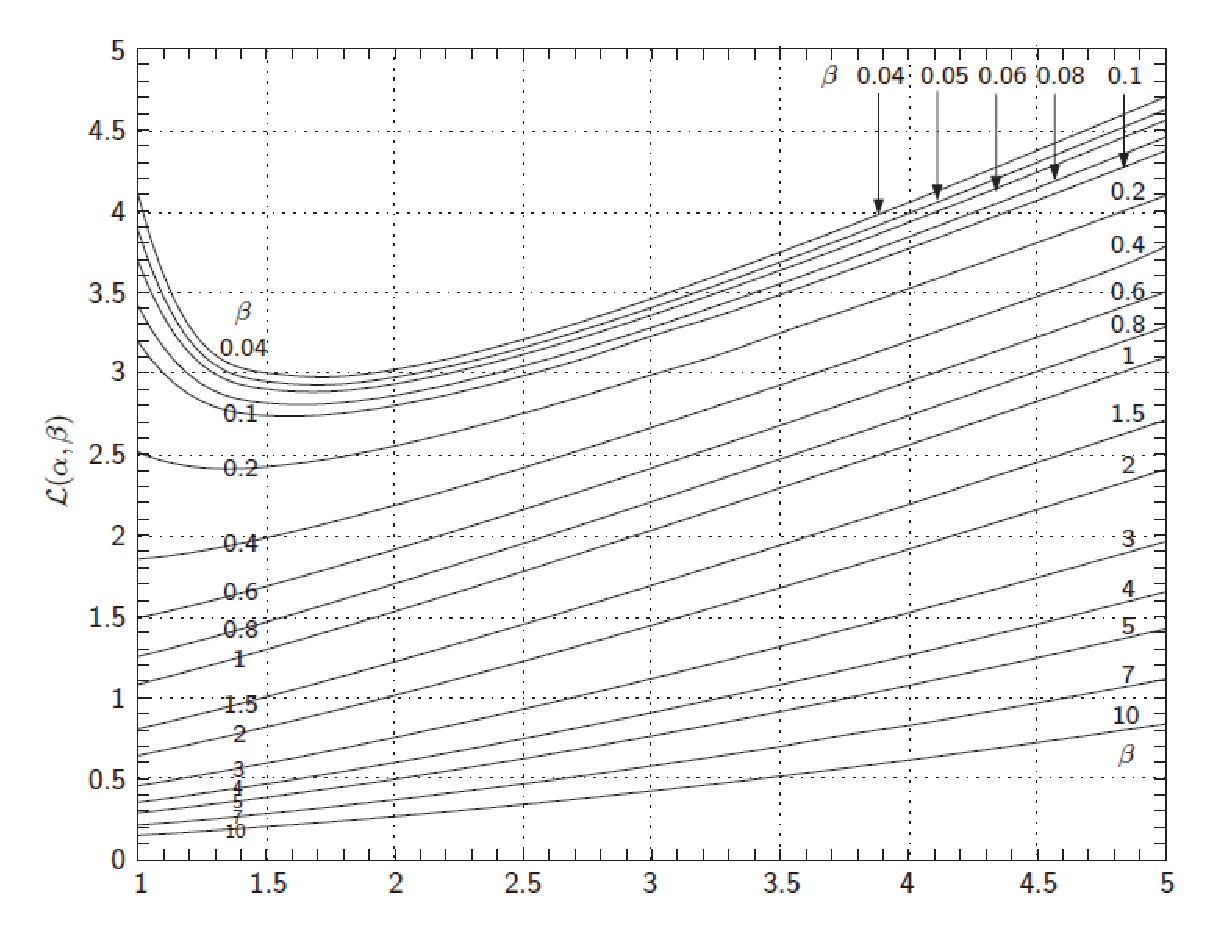
\includegraphics[scale=0.7]{chpt3/figs/fig3.14.eps}
  \caption{螺管线圈参数为$\alpha,\beta$时的$\mathcal{L}(\alpha,\beta)$}
\end{figure}

对于一个``薄壁"螺管,即$\alpha\simeq 1,\beta\rightarrow \infty$,3.82b简化为$\pi/2\beta$。
问题3.18将给出详细推导。

\subsection{实用电感公式}
本节给出无磁性材料($\mu=\mu_0$)线圈的实用电感公式。
一些公式的推导,在问题3.18中会再次涉及。

在有可方便实用的电感计算程序之前,人们推导了``厚壁"绕组电感的解析表达式,在工程手册中可以找到。
这些公式一般来说是很难用的。对大多数应用,图3.14或者式3.82对电感计算已足够,特别是早期设计阶段。

\textbf{导线}  
  
半径为$a$的导线,单位长度电感$L$[H/m]为:
  \begin{equation}
         L=\frac{\mu_0}{8\pi}%page108
  \end{equation}
  
\textbf{``长"线圈} 
  
  a. 一个``长"$(\beta>0.75)$、``薄壁"(内径$2a_1$)$N$匝线圈[3.7]:
\begin{equation}
  L=\mu_0a_1N^2\left[\frac{\pi(1+\alpha)^2}{8\beta}\right]\left[1-\frac{2}{3\pi\beta}+\frac{(1+\alpha)^2}{32\beta^2}...\right]%page108
\end{equation}

在$(\alpha−1)/(\alpha+1)\ll 1$时,式3.84成为:
\begin{equation*}
  L=\mu_0a_1N^2\left(\frac{\pi}{2\beta}\right)\left[1-\frac{2}{3\pi\beta}+\frac{1}{8\beta^2}...\right] \tag{3.84b}%page108
\end{equation*}

b.一个``很长"($\beta\gg 1$)且``薄壁"($\alpha \simeq 1$)的线圈,式3.84b成为:
\begin{equation*}
  L=\mu_0a_1N^2\left(\frac{\pi}{2\beta}\right) \tag{3.84c}%page108
\end{equation*}

可见,对一个非常长且薄壁的线圈,有$\mathcal{L}(\alpha,\beta)=\pi/2\beta$。

\textbf{``短"线圈}

 一个``短"$(\beta<0.75)$、``薄壁"(内径$2a_1,\alpha\simeq 1$) 的$N$匝线圈[3.7]:
\begin{equation}
L\simeq \mu_0a_1N^2\left(\frac{\alpha+1}{2}\right)\left(\ln\left\{\left[\frac{2(\alpha+1)}{\beta}\right]\left[1+\frac{\beta^2}{2(1+\alpha^2)}\right]\right\}-\frac{1}{2}\left[1+\frac{\beta^2}{4(1+\alpha^2)}\right]\right)
\end{equation}
  
  如果$\beta \ll 1$,则有:
  \begin{equation*}
L\simeq\mu_0a_1N^2\left(\frac{\alpha+1}{2}\right)\left\{\ln\left[\frac{2(\alpha+1)}{\beta}\right]-0.5\right\} \tag{3.85b}%page108
\end{equation*}

\textbf{``饼式''(扁平)线圈}

一个内径为$2a_1$的饼式(扁平)($\beta\ll 1$)$N$匝线圈[3.7]:
  \begin{equation}
  \begin{split}
L\simeq & \mu_0a_1N^2\left(\frac{\alpha+1}{2}\right)\bigg\{\ln\left[\frac{4(\alpha+1)}{\alpha-1}\right]\left[1+\frac{1}{24}\frac{(\alpha-1)^2}{(\alpha+1)^2}\right]\\
&-\frac{1}{2}\left[1-\frac{43}{144}\frac{(\alpha-1)^2}{(\alpha+1)^2}\right]\bigg\}%page10
  \end{split}
\end{equation}

当$(\alpha-1)/(\alpha+1)\ll 1$时,上式进一步简化为:
\begin{equation*}
L\simeq\mu_0a_1N^2\left(\frac{\alpha+1}{2}\right)\left\{\ln\left[\frac{4(\alpha+1)}{\alpha-1}\right]-0.5\right\} \tag{3.86b}%page109
\end{equation*}

注意到,对于``环"线圈($N=1$),有$a_1(\alpha+1)=2R$(环直径)和$2a_1\beta=2a$
或$a_1(\alpha-1)=2a$(导线直径),式3.85b和3.86b都将简化为:
\begin{equation*}
L\simeq\mu_0 R\left[\ln\left(\frac{4R}{a}\right)-0.5\right]=\mu_0 R\left[\ln\left(\frac{R}{a}\right)+0.886\right] \tag{3.86c}
\end{equation*}

具有\textit{长方形}截面的环线圈用式3.86c,\textit{圆形}截面的环用式3.80a。
对一个很平($\alpha\gg 1$)的饼式线圈,3.86可以进一步简化为:
\begin{equation*}
L  \simeq  0.5\mu_0a_1\alpha N^2\left\{\ln\left(\frac{25}{6}\right)-\frac{101}{288}\right\}=0.538\mu_0a_1\alpha N^2\approx 0.5\mu_0a_2N^2 \tag{3.86d}
\end{equation*}

注意,3.86d中出现的是$a_2$而\textit{不}是$a_1$。

\textbf{``理想''二极磁体}

有$N$匝绕组的``理想"二极磁体(问题3.8)---无限长、零绕组厚度---的\textit{单位长度电感}${L_\ell}$[H/m]为:
\begin{equation}
L_\ell=\frac{1}{8}\mu_0\pi N^2%page109
\end{equation}

\textbf{``理想''四极磁体}

有$N$匝绕组的``理想"四极磁体(问题3.9)---无限长、零绕组厚度---的\textit{单位长度电感}${L_\ell}$[H/m]为:
\begin{equation}
L_l=\frac{1}{16}\mu_0\pi N^2 %page109
\end{equation}

可见,理想二极磁体和理想四极磁体的电感均与绕组半径无关,但与长度成正比。

\textbf{``理想''圆截面的螺绕环}

有$N$匝绕组的``理想"圆截面螺绕环磁体(问题3.10)---零绕组厚度、主半径$R$,圆截面半径$a$---的电感:
  \begin{equation}
 L=\mu_0RN^2\left[1-\sqrt{1-\left(\frac{a}{R}\right)^2}\right]%page110
\end{equation}

在极限$a\ll R$下,$L$近似为:
\begin{equation*}
 L=\mu_0aN^2\left(\frac{a}{2R}\right)\left[1+\frac{1}{4}\left(\frac{a}{R}\right)^2+\frac{1}{8}\left(\frac{a}{R}\right)^4+\cdots\right]\simeq\mu_0aN^2\left(\frac{a}{2R}\right) \tag{3.89b}%page110
\end{equation*}

\textbf{``理想"矩形截面的螺绕环}

有$N$匝绕组的``理想"矩形截面螺绕环磁体---零绕组厚度,主半径$R$,矩形截面$r$轴宽$2a$、$z$轴高$2b$---的电感:
 \begin{equation}
L=\mu_0bN^2\left[\frac{1}{\pi}\ln\left(\frac{R+a}{R-a}\right)\right]%page110
\end{equation}

在极限$a\ll R$下,$L$近似为:
\begin{equation*}
L=\mu_0bN^2\left(\frac{2a}{\pi R}\right)\left[1+\frac{1}{3}\left(\frac{a}{R}\right)^2+\frac{1}{5}\left(\frac{a}{R}\right)^4+\cdots\right]\simeq\mu_0bN^2\left(\frac{2a}{\pi R}\right) \tag{3.90b}%page110
\end{equation*}



%%%%第3.8节
\section{互感}
当两个线圈1和2相互靠近时,他们之间通常会存在电感相互作用。
他们的耦合可以定量的用互感$M_{12}$或$M_{21}$描述,且有$M_{12}=M_{21}=M$。于是:
\begin{equation}
M_{12}\equiv N_1\frac{\Phi_{12}}{I_2}=M_{21}\equiv N_2\frac{\Phi_{21}}{I_1}%page111
\end{equation}
式中,$\Phi_{12}$是当线圈2通过电流$I_2$产生的磁通与线圈1的$N_1$匝的交链;
$\Phi_{21}$是当线圈1通过电流$I_1$产生的磁通与线圈2的$N_2$匝的交链。

两线圈耦合系统的总磁能$E_m$为:
\begin{equation}
\begin{split}
E_m&=\frac{1}{2}L_1I_1^2+\frac{1}{2}L_2I_2^2+\frac{1}{2}M_{12}I_1I_2+\frac{1}{2}M_{21}I_1I_2\\
&= \frac{1}{2}L_1I_1^2+\frac{1}{2}L_2I_2^2+M_{12}I_1I_2%page111
\end{split}
\end{equation}

和自感公式类似,一些特定的线圈可以写出互感表达式。
用来计算我们感兴趣的线圈系统(如耦合的同轴螺管线圈组)的线圈自感的程序,
通常能计算多线圈系统的电感矩阵。

\textbf{串联线圈} 
  
  两个自感为$L_1,L_2$互感为$M_{12}$的两线圈,串联后的有效自感$L_s$为:
  \begin{equation}
   L_s=L_1+L_2 \pm 2M_{12}%page111
  \end{equation}

如果两者的磁场是加强的,$M_{12}$取$+$号;反之,取$−$号。

\textbf{并联线圈} 

两个自感为$L_1,L_2$互感为$M_{12}$的两线圈,并联后的有效自感$L_s$为:
  \begin{equation}
L_p=\frac{L_1 L_2-M_{12}^2}{L_1+L_2 \mp 2M_{12}}%page111
\end{equation}

\textbf{互感系数} 

互感$M_{12}$与$L_1,L_2$有关:
\begin{subequations}
	\begin{align}
M_{12}=&k\sqrt{L_1L_2}\\%page111
k=&\frac{M_{12}}{\sqrt{L_1L_2}}%page111
	\end{align}
\end{subequations}
其中,$k$称为耦合系数;$k=0$表示线圈间无耦合,$k=1$表示全耦合。
对于一对紧密嵌套的螺管线圈,即一个线圈同轴、同心、中平面对齐的放置于位于另一个线圈的室温孔内,
$k$一般在$0.3-0.6$。当他们的$\alpha$和$\beta$相近时,趋向于0.6;否则,趋向于0.3。


\subsection{互感---几个解析表达式}
因为线圈之间的力和互感是紧密相连的,前面给出的线圈A和线圈B之间的轴向力解析表达式可以用于导出互感公式。
根据$\vec{F}=I_A I_B \nabla M$,显然M的表达式要比轴向力的表达式更复杂。因此,下面仅讨论几个简单的例子。

\textbf{两个``环"线圈间的互感} 

两个轴对齐的``环"线圈A($2a_A,N_A$)和线圈B($2a_B,N_B$)相距$\rho$,其互感$M_{AB}(\rho)$为:
  \begin{equation}
M_{AB}=\frac{\mu_0}{2}(N_AN_B)\sqrt{(a_A+a_B)^2+\rho^2}\left\{2[K(k)-E(k)]-k^2K(k)\right\}%page112
\end{equation}
本系统的模量$k^2$为:
\begin{equation*}
k^2=\frac{4a_Aa_B}{(a_A+a_B)^2+\rho^2}%page112
\end{equation*}

\textbf{特例1:相距很远的两个环形线圈} 

  当两个环线圈相距很远时,即$\rho^2\gg(a_A+a_B)^2$或$k^2\ll 1$时,可以用式3.38c和3.38a来简化3.96:
\begin{equation}
M_{AB}\simeq\frac{\mu_0}{2\pi}\left[\frac{(\pi a_A^2N_A)(\pi a_B^2N_B)}{\rho^3}\right]\\%page112
\end{equation}

上式表明,互感近似正比于两个线圈的总绕组面积---$\pi a_A^2 N_A$和$\pi a_B^2 N_B$---之积除以$\rho^3$。

\textbf{``薄壁''螺管线圈和环线圈间的互感} 

  此处,我们考虑一个``薄壁"螺管($2a_S$;均匀匝密度$N_S/2b_S$)和一个环线圈($2a_R,N_R$),
  两者在轴向对齐,环线圈位于螺管右端右侧$\rho$处,如图3.6所示。
  螺管线圈和环线圈间的互感$M_{RS}$为:
  \begin{equation}
  \begin{split}
M_{RS}(\rho)=&-\frac{\mu_0}{2}\left(\frac{N_RN_S}{2b_S}\right)\times\\
&\bigg(\frac{\rho}{\sqrt{(a_R^2+a_S^2)^2+\rho^2}}\{[(a_R+a_S)^2+\rho^2][K(k_R)-E(k_R)]-\gamma(c^2,k_R)\}\\
&-\frac{2b_S+\rho}{\sqrt{(a-R+a_S)^2+(2b_S+\rho)^2}}\times
\{[(a_R+a_S)^2+(2b_S+\rho)^2][K(k_S)-E(k_S)]-\gamma(c^2,k_S)\}\bigg)%page112
  \end{split}
\end{equation}
式中,
\begin{equation*}
k_R^2=\frac{4a_Ra_S}{(a_R+a_S)^2+\rho^2};\quad k_S^2=\frac{4a_Ra_S}{(a_R+a_S)^2+(2b_S+\rho)^2};\quad c^2=\frac{4a_Ra_S}{(a_R+a_S)^2}%page112
\end{equation*}

\textbf{特例2:相距很远的薄壁螺管和环线圈} 

当两个线圈很远,至于满足$k_R^2 \ll 1, k_S^2\ll 1,\rho > b_S$时,式3.98可简化为:
\begin{align}
M_{RS} = \frac{\mu_0}{2} \left(\frac{N_RN_S}{2b_S}\right) 
\left\{\frac{2\pi(a_R a_S)^2 b_S}{\rho^3}\left(1+\frac{b_S}{\rho}\right)
-(a_R-a_S)^2[\prod(c^2,k_S)-\prod(c^2,k_S)]\right\}
\end{align}
  
尽管$\rho$比$a_R$和$a_S$长不少,但仍能远大于$b_S$。于是,``修正''项$b_S/\rho$和$\prod(c^2, k)$在3.99中还必须予以保留。

\textbf{特例3:相距极远的薄壁螺管和环线圈} 

  当两个线圈足够远,至于$\rho \gg b_S$以及$k_R\rightarrow 0,k_S\rightarrow 0$都满足时,3.99可进一步简化为:
 \begin{equation}
\begin{split}
M_{RS}&=\frac{\mu_0}{2}\left(\frac{N_RN_S}{2b_S}\right)\frac{2\pi(a_Ra_S)^2b_S}{\rho^3}\\
&=\frac{\mu_o}{2\pi}(\pi a_R^2N_R)\left(\frac{\pi a_S^2N_S}{2b_S}\right)\frac{2b_S}{\rho^3}%page113
\end{split}
\end{equation}

\textbf{环线圈位于薄壁螺管的中部} 

\begin{figure}[htbp]
	\centering
	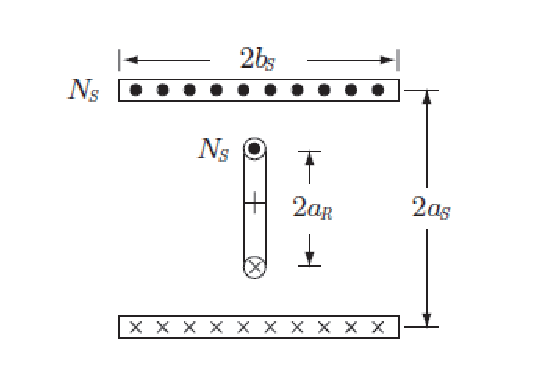
\includegraphics[scale=0.7]{chpt3/figs/fig3.15.eps}
	\caption{环形线圈置于薄壁螺管线圈的中平面处。}
\end{figure}

图3.15给出了两个线圈的位置示意。图中环线圈位于薄壁螺管线圈的中平面。
此时,$\rho=-b_S$。将$\rho=-b_S$代入式3.98,我们得到下面的简化表达式:
  \begin{equation}
  \begin{split}
M_{RS}(\rho=-b_S)\simeq & \frac{\mu_0}{2}\left(\frac{N_R N_S}{2b_S}\right)\times\frac{2b_S}{\sqrt{(a_R+a_S)^2+b_S^2}}\times\\
&\left\{[(a_R+a_S)^2+b_S^2][K(k)-E(k)]-\Upsilon(c^2,k)\right\}
\end{split}
\end{equation}
式中,$k$为:
  \begin{equation*}
k^2=\frac{4a_Ra_S}{(4a_R+a_S)^2+b_S^2}
\end{equation*}

\textbf{特例4:``长''薄壁螺管和环线圈} 

当薄壁螺管线圈是``长"的,特别是当$b_S\gg a_R$和$b_S\gg a_S$满足时,
环线圈和螺管线圈的相对位置不再重要。
对于满足$k^2\simeq 4a_R a_S/b_S^2$的长螺管,式3.101变为:
\begin{align}
M_{RS}&\simeq\frac{\mu_0}{2}\left(\frac{N_RN_S}{2b_S}\right)(2)\left\{b_S^2[K(k)-E(k)]-\Upsilon(c^2,k)\right\}\\\notag
&\simeq\frac{\mu_0}{2}\left(\frac{N_RN_S}{2b_S}\right)\pi(a_R^2+a_S^2)\left[1-\frac{2(a_R-a_s)^2}{\pi(a_R^2+a_S^2)}\prod(c^2,k)\right] 
\end{align}

式3.102的方括号内的第二项可以视为修正项,在极限$ a_R\gg a_S$或$a_R\ll a_S$时可以忽略。

\textbf{特例5:与螺管直径相差很大的环线圈} 

当环线圈的直径与螺管线圈直径相差很大时,条件$c^2\rightarrow 0$满足,
前已提及(式3.49b),$\prod(c^2,0)$可由依$c^2$展开的级数的前几项表示。
在极限$k^2\rightarrow 0(b_S\gg a_R,b_S\gg a_S)$时,3.102中的$\prod(c^2,k)\rightarrow \prod(c^2,0)$。
使用3.49b,有:
  \begin{align}
M_{RS}&\simeq\frac{\mu_0}{2}\left(\frac{N_RN_S}{2b_S}\right)\pi(a_R^2+a_S^2)\left[1-\frac{(a_R-a_S)^2}{(a_R^2+a_S^2)}(1+\frac{1}{2}c^2+\frac{3}{8}c^4+\frac{5}{16}c^6)\right]\\\notag
&\simeq\frac{\mu_0}{2}\left(\frac{N_RN_S}{2b_S}\right)\pi(a_R^2+a_S^2)\times \\\notag
&\left\{1-\frac{(a_R-a_S)^2}{(a_R^2+a_S^2)}\left[1+\frac{2a_Ra_S}{(a_R^2+a_S^2)^2}+\frac{6(a_Ra_S)^2}{(a_R^2+a_S^2)^4}+\frac{20(a_Ra_S)^3}{(a_R^2+a_S^2)^6}\right]\right\}%page114
\end{align}

\subsection{互感和相互作用力}

使用3.5.7节导出的轴向偏心线圈受到的轴向恢复力表达式,
我们可以导出两个线圈的互感表达式与轴向的关系。
两个螺管A、B间的净磁场力$\vec{F}_{AB}$与两个线圈中储存的总磁能有关:
\begin{equation}
\vec{F}_{AB}=\nabla E_{AB}%page114
\end{equation}

将式3.92中的下标替换为A和B,代入3.104a,并注意到$z$向的$F_{AB}$就是式3.60给出的$F_{ZR}(\rho)$,我们有:
\begin{equation}
F_{zR}(\rho)=\frac{\partial E_{AB}}{\partial \rho}=I_AI_B\frac{\partial M_{AB}(\rho)}{\partial \rho}%pagr114
\end{equation}

对于小距离$\rho$($\rho\ll \sqrt{a_T^2+b_D^2}$),我们可以对式3.61给出的$F_{ZR}(\rho)$积分:
\begin{equation}
M_{AB}(\rho)-M_{AB}(0)\propto-\rho^2%page114
\end{equation}

可见,对于小距离$\rho$,$M_{AB}(\rho)$随偏离中心距离的平方($\rho^2$)减小。 

\subsection*{磁场强度$H$和磁感应强度$B$}

除非特别指明,专题中的磁体都是空心的。此时,磁感应强度$B$和磁场强度$H$存在简单关系:$B=\mu_0 H$。
其中,$\mu_0$是空气磁导率,约等于真空磁导率$\mu_0=4\pi\times 10^{-7}$ H/m。
通常在SI单位制下,常用特斯拉[T]作磁感应强度$B$的单位,用安培每米[A/m]作磁场强度$H$的单位;工程师通常这么使用。在一些文献中常遇到用$B$代替$H$的,主要原因是:
1) 在cgs电磁单位制下,$B$[gauss]和$H$[oersted]在数值上相等;
2) gauss比oersted更常用。在第二版中,把第一版中使用$H$来表达的方程式都改用$B$给出了。

\newpage
\section{专题}
\subsection{讨论3.1:均匀电流密度螺管}

这里,我们首先讨论均匀电流密度螺管线圈的一些基本问题。
绕组内径i.d.为$2a_1$,外径o.d.为$2a_2$,总长度是$2b$。
图3.16定义了绕组截面---因为我们处理的是轴对称螺管,仅考虑$z$和$r$轴。
由位于$(r,z)$处的载流环微元$dA\mathrm{[A/m^2]}$在中心点处产生的磁场$dB_z(0, 0)$[T]可由式3.3a的等价形式给出:
\begin{equation}
dB_z(0,0)=\frac{\mu_0r^2\lambda JdA}{2(r^2+z^2)^\frac{3}{2}}%page115
\end{equation}
式中,$\lambda J\mathrm{[A/m^2]}$是微元内部的总电流密度。
无量纲数$\lambda$称为空间因子,它刻画了绕组截面并非完全由载流导体占据这一事实。
注意到在这个模型中,$\lambda J$在整个绕组截面上是均匀的,且有:
\begin{subequations}
\begin{align}
\lambda J&=\frac{NI}{2b(a_2-a_1)}\\
&=\frac{NI}{2a_1^2\beta(\alpha-1)}%page115
\end{align}
\end{subequations}
式中,$\alpha=a_2/a_1,\beta=b/a_1$。$N$是总匝数,$NI$称为总安匝数。
\begin{figure}[htbp]
  \centering
 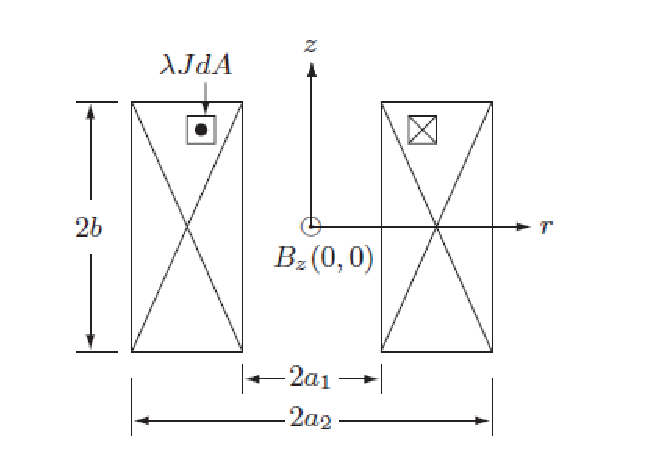
\includegraphics[scale=0.7]{chpt3/figs/fig3.16.eps}
  \caption{均匀电流密度螺管的截面。}
\end{figure}

对3.107式依次从$r=a_1$到$r=a_2$以及从$z=-b$到$z=b$积分,
我们得到螺管的$B_z(0,0)$的表达式,在3.4节中它是由3.13a的$H_z(0,0)$和
3.13b的磁场因子$F(\alpha,\beta)$给出的:
\begin{equation}
B_z(0,0)=\mu_0\lambda J_{a_1}F(\alpha,\beta)\\ %page116
\end{equation}
\begin{equation*}
F(\alpha,\beta)=\beta \ln\left(\frac{\alpha+\sqrt{\alpha^2+\beta^2}}{1+\sqrt{1+\beta^2}}\right) \tag{3.13b}
\end{equation*}

前已提及,$F(\alpha,\beta)$是均匀电流密度线圈的``场因子"。
和式3.81给出的电感参数$\mathcal{L}(\alpha,\beta)$类似,它也仅依赖于螺管线圈的截面形状。
图3.17给出了三组有关$F(\alpha,\beta)$的关系:3.17a是$\beta$为常数时,$F(\alpha,\beta)$与$\alpha$的关系;3.17b是$\alpha$为常数时,$F(\alpha,\beta)$与$\beta$的关系;3.17c是$F(\alpha,\beta)$为常数时,$\beta$与$\alpha$的关系[3.8]。

与$F(\alpha,\beta)$类似,螺管中的导体总体积$\mathcal{V}_{cd}=\lambda 2\pi a_1^3(\alpha^2-1)\beta$在给定的$\lambda$和$a_1$条件下仅依赖于$\alpha,\beta$:
每一幅图中的实线上的点都是给定$F(\alpha,\beta)$下的\textit{最小}导体体积。
$F(\alpha,\beta)$与某些\textit{特殊}线圈相关的显著特征将在问题3.1中论及。

\begin{figure}[htbp]
	\centering
	\subfigure[在$\beta$为常数时,$F(\alpha,\beta)$与$\alpha$的关系(虚线)。实线表示给定$F(\alpha,\beta)$下的最小导体体积。]
	{
		\label{fig:subfig:a} %% label for first subfigure
		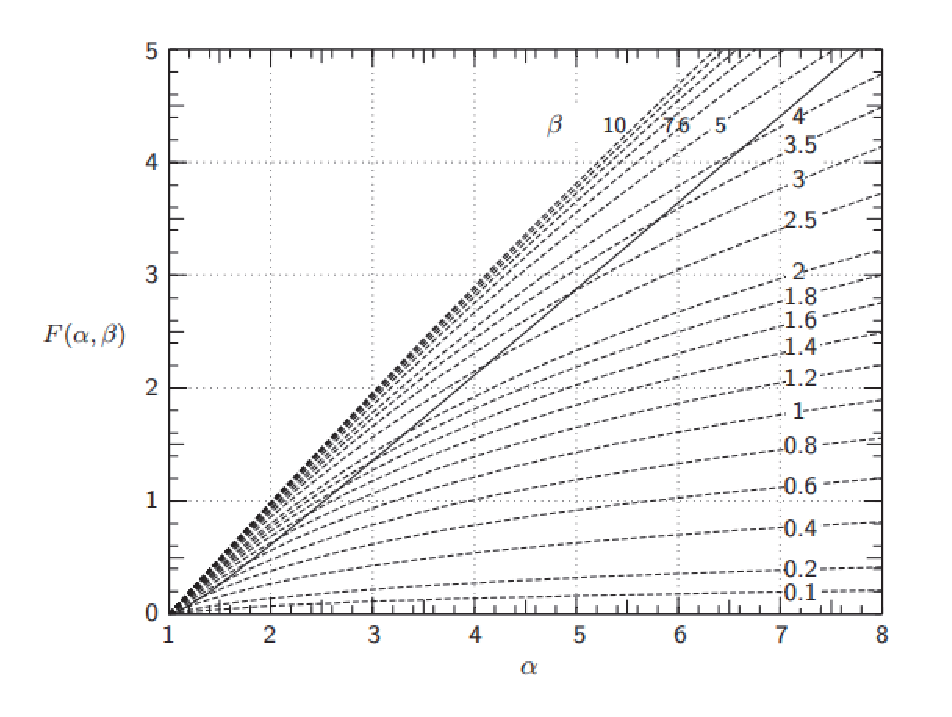
\includegraphics[scale=0.6]{chpt3/figs/fig3.17a.eps}}

	\subfigure[在$\alpha$为常数时,$F(\alpha,\beta)$与$\beta$的关系(虚线)。实线表示给定$F(\alpha,\beta)$下的最小导体体积。]
	{
		\label{fig:subfig:b} %% label for second subfigure
		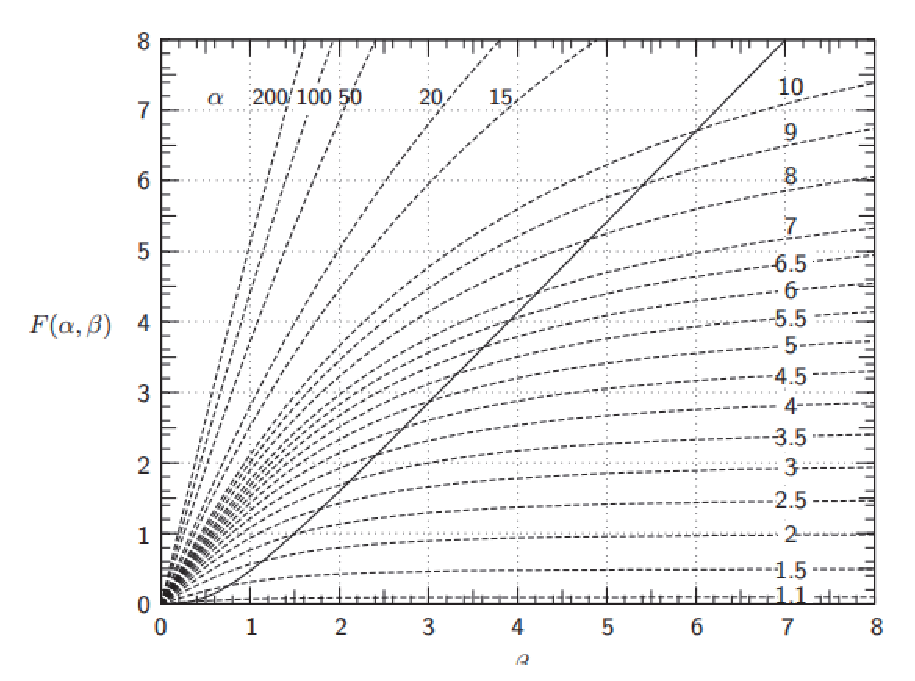
\includegraphics[scale=0.6]{chpt3/figs/fig3.17b.eps}}
	\subfigure[在$F(\alpha,\beta)$为常数时,$\beta$与$\alpha$的关系(虚线)。实线表示给定$F(\alpha,\beta)$下的最小导体体积。]
	{
		\label{fig:subfig:c} %% label for second subfigure
		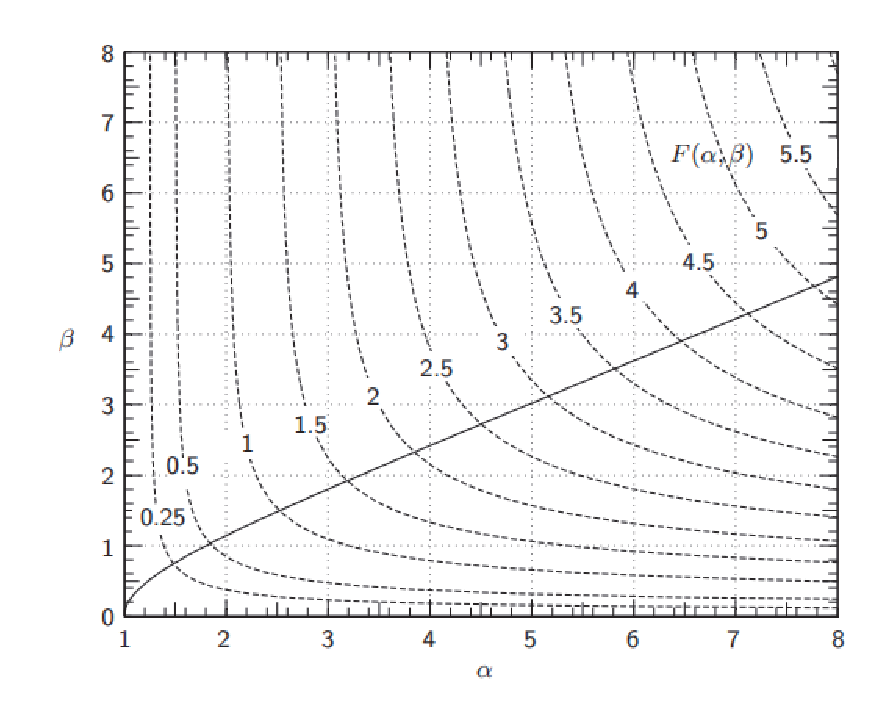
\includegraphics[scale=0.6]{chpt3/figs/fig3.17c.eps}}
	
	\caption{$F(\alpha,\beta)$、$\beta$、$\alpha$之关系}
	\label{fig:subfig} %% label for entire figure
\end{figure}

\subsection{问题3.1:``简单"螺管线圈}
a) 由式3.107推导出式3.109和3.13b。

b)通过联立3.108b和3.109,我们还可以将$B_z(0,0)$表示为:
\begin{equation}
B_z(0,0)=\frac{\mu_0NI}{2a_1(\alpha-1)}\ln\left(\frac{\alpha+\sqrt{\alpha^2+\beta^2}}{1+\sqrt{1+\beta^2}}\right)%page118
\end{equation}

\begin{description}
  \item[``环"线圈] 对半径为$a_1$、总载流为$NI$的``环''线圈($\alpha=1$),式3.110可化简为:
  \begin{equation}
    B_z(0,0)=\frac{\mu_0NI}{2a_1}%page118
  \end{equation}
 \item[``薄壁"螺管] 对``薄壁''螺管($\alpha \rightarrow 1$),式3.110可化简为:
 \begin{align*}
   B_z(0,0)=\frac{\mu_0NI}{2a_1}\left(\frac{1}{\sqrt{1+\beta^2}}\right)\tag{3.111b}\\ %page118
 \end{align*}
  同时证明:
 \begin{align*}
   B_z(0,0)=\mu_0 \lambda Ja_1(\alpha-1)\frac{\beta}{\sqrt{1+\beta^2}}\tag{3.111c}%page118
 \end{align*}
  \item[``长"螺管] 对于长度远大于外直径的螺管($\beta \gg \alpha$),式3.110可化简为:
\begin{equation*}
B_z(0,0)=\frac{\mu_0NI}{2b} \tag{3.111d}%page118
\end{equation*}

因为$NI/2b=K_\theta$,式3.111d等价于式3.5。同时,证明:
\begin{equation*}
B_z(0,0)=\mu_0\lambda Ja_1(\alpha-1) \tag{3.111e}%page118
\end{equation*}
  \item[``饼式"线圈] 对于长度比外直径小很多的饼式线圈,式3.110可化简为:
  \begin{equation*}
B_z(0,0)=\frac{\mu_0NI}{2a_1}\left(\frac{\ln\alpha}{\alpha-1}\right) \tag{3.111f}%page118
  \end{equation*}

式3.111f将在讨论3.6进一步研究。
\end{description}

c) \textbf{场和能量}:证明\textit{电阻性}螺管(比如铜螺管)的中心场$B_z(0,0)$与其所需功率$P$的关系为:
\begin{subequations}
	\begin{align}
B_z(0,0)=&\mu_0G(\alpha,\beta)\sqrt{\frac{\lambda P}{\rho_{cd}a_1}}\\ %page118
G(\alpha,\beta)=&\sqrt{\frac{\beta}{2\pi(\alpha^2-1)}}\ln\left(\frac{\alpha+\sqrt{\alpha^2+\beta^2}}{1+\sqrt{1+\beta^2}}\right)%page118
	\end{align}
\end{subequations}
式中,$\rho_{cd}$是导体的电导率。$G(\alpha,\beta)$称为均匀电流密度线圈的``G因子"[3.2]。

\subsubsection{问题3.1之解}

a) 对式3.107在$z$和$r$的合适区间积分,得:
\begin{equation*}
B_z(0,0)=\frac{\mu_0\lambda J}{2}\int_{a_1}^{a_2}\int_{-b}^{b}\frac{r^2dzdr}{(r^2+z^2)^{3/2}}=\mu_0\lambda J\int_{a_1}^{a_2}\int_{0}^{b}\frac{r^2dzdr}{(r^2+z^2)^{3/2}}%page119
\end{equation*}

查积分表,得:
\begin{equation*}
\int_{0}^{b}\frac{dz}{(r^2+z^2)^{3/2}}=\left[\frac{z}{r^2\sqrt{r^2+z^2}}\right]_{0}^{b}=\frac{b}{r^2\sqrt{r^2+b^2}}%page119
\end{equation*}

于是:
\begin{equation*}
\begin{split}
B_z(0,0)&=\mu_0\lambda J\int_{a_1}^{a_2}\frac{r^2bdr}{r^2\sqrt{r^2+b^2}}=\mu_0\lambda Jb\left[\ln({r+\sqrt{r^2+b^2}})\right]_{a_1}^{a_2}\\
&=\mu_0\lambda Jb\left[\ln(a_2+\sqrt{a_2^2+b^2})-\ln(a_1+\sqrt{a_1^2+b^2})\right]\\
&=\mu_0\lambda Ja_1\left(\frac{b}{a_1}\right)\ln\left[\frac{\frac{a_2}{a_1}+\sqrt{(\frac{a_2}{a_1})^2+(\frac{b}{a_1})^2}}{(\frac{a_1}{a_2})+\sqrt{(\frac{a_1}{a_1})^2+(\frac{b}{a_1})^2}}\right]\\%page119
\end{split} \tag{S1.1}
\end{equation*}

代入$a_2/a_1=\alpha$和$b/a_1=\beta$,式S1.1变为:
\begin{equation*}
B_z(0,0)=\mu_0\lambda J\alpha_1\beta\ln\left[\frac{\alpha+\sqrt{\alpha^2+\beta^2}}{1+\sqrt{1+\beta^2}}\right]\tag{S1.2}
\end{equation*}

于是:
\begin{align*}
B_z(0,0)=&\mu_0\lambda J {a_1} F(\alpha,\beta)\tag{3.109}\\ %page119
F(\alpha,\beta)=&\beta \ln\left(\frac{\alpha+\sqrt{\alpha^2+\beta^2}}{1+\sqrt{1+\beta^2}}\right)\tag{3.13b}%page119
\end{align*}

b) \textbf{``环"线圈}。对环线圈($\alpha\rightarrow 1; \beta\rightarrow 0$),
式3.110等号右侧的对数项成为:
\begin{equation*}
\lim_{\beta\rightarrow 0}\ln\frac{\alpha+\sqrt{\alpha^2+\beta^2}}{1+\sqrt{1+\beta^2}}=\ln\alpha%page119
\end{equation*}

因为当$|\epsilon|\ll 1$时,$\ln (1+\epsilon)\simeq \epsilon$。故有$\alpha\rightarrow 1$时,$\ln \alpha\rightarrow \alpha-1$。于是:
\begin{equation*}
B_z(0,0)=\frac{\mu_0NI}{2a_1(\alpha-1)}(\alpha-1)=\frac{\mu_0NI}{2a_1}\tag{3.111}%page119
\end{equation*}

注意式3.111a和3.3a的关系。式3.3a在$z=0$时用$a_1,NI$分别替换$a,I$,将得到3.111a(除$\mu_0$项)。

\textbf{``薄壁''螺管。}对薄壁螺管($\alpha\rightarrow 1$),联立3.13b和3.23b,可得:
\begin{equation*}
\lim_{\alpha\rightarrow 1}\ln\frac{\alpha+\sqrt{\alpha^2+\beta^2}}{1+\sqrt{1+\beta^2}}=\frac{\alpha-1}{\sqrt{1+\beta^2}} \tag{S1.3}%page120
\end{equation*}

联立3.110和S1.3,得3.111b;联立3.109,3.13b和S1.3,得3.111c:
\begin{align*}
B_z(0,0)&=\frac{\mu_0 NI}{2a_1}\left(\frac{1}{1+\beta^2}\right)\tag{3.111b}\\ %page120
B_z(0,0)&=\mu_0 \lambda Ja_1(\alpha-1)\frac{\beta}{\sqrt{1+\beta^2}}\tag{3.111c}%page120
\end{align*}

注意到,对于``长''`螺管($\beta\gg 1$),3.111c变成3.111e。

\textbf{``长''螺管。}在$\beta\gg \alpha$时,有:
\begin{equation*}
\lim_{\beta\gg\alpha}\ln\left(\frac{\alpha+\sqrt{\alpha^2+\beta^2}}{1+\sqrt{1+\beta^2}}\right)=\ln\left(\frac{\alpha+\beta}{1+\beta}\right)=\ln\left(\frac{\frac{\alpha}{\beta}+1}{\frac{1}{\beta}+1}\right)%page120
\end{equation*}

使用推导``环"线圈采用近似方法,得:
\begin{equation*}
\lim_{\beta\gg\alpha}\ln\left(\frac{\frac{\alpha}{\beta}+1}{\frac{1}{\beta}+1}\right)\simeq\frac{\alpha}{\beta}-\frac{1}{\beta}=\frac{\alpha-1}{\beta}%page120
\end{equation*}

在极限$\beta\gg\alpha$下,得:
\begin{equation*}
B_z(0,0)=\frac{\mu_0NI}{2b} \tag{3.111d}%page120
\end{equation*}

上文已提及,$NI/2b$可以视为表面电流密度。
根据式3.108,$NI/2b=\lambda J (a_2-a_1)$。于是式3.111d又可以写为:
\begin{equation*}
B_z(0,0)=\mu_0\lambda Ja_1(\alpha-1) \tag{3.111e}%page120
\end{equation*}

长螺管的中心场与其长度($\beta$)无关---
$B_z(0,0)$在大$\beta(>\sim 3)$和中等$\alpha(<\beta)$情况下的独立性从图3.17b清晰可见。
由图3.17a可见,在大$\beta$和中等$\alpha(<\beta)$情况下,
$B_z(0,0)$正比于线圈的$a_2-a_1$。这是因为该值越大,相应的单位长度总安匝数越大。

\textbf{``饼式''线圈。} 对饼式线圈,极限条件是$\beta\rightarrow 0$:
\begin{align*}
&\lim_{\beta\rightarrow 0}\ln\frac{\alpha+\sqrt{\alpha^2+\beta^2}}{1+\sqrt{1+\beta^2}}=\ln\left(\frac{2\alpha}{2}\right)=\ln\alpha\notag \\%page120
&B_z(0,0)=\frac{\mu_0NI}{2a_1}\left(\frac{\ln\alpha}{\alpha-1}\right) \tag{3.111f}%page120
\end{align*}

注意到,饼式线圈的中心场等于``环''线圈的中心场乘一个系数$\ln \alpha/(\alpha-1)$。
在$\alpha\rightarrow 1$时,式3.111f退化为3.111a。

c) 总导体体积等于$\lambda\times$<绕组体积(winding volume, wv)>:
\begin{equation*}
<\mathrm{wv}>=2b\pi(a_2^2-a_1^2)=a_1^32\pi\beta(\alpha^2-1)%page121
\end{equation*}

于是:
\begin{equation*}
P=\rho_{cd}J^2\lambda a_1^32\pi\beta(\alpha^2-1) \tag{3.112}%page121
\end{equation*}
式中,$J$是仅存在于导体中的电流密度。由式3.112,我们用$P$和其他参数解出$J$:
\begin{equation*}
J=\sqrt{\frac{P}{\rho_{cd}\lambda a_1}}\left[\frac{1}{a_1\sqrt{2\pi\beta(\alpha^2-1)}}\right]\tag{S1.4}%page121
\end{equation*}

联立S1.2和S1.4,得到:
\begin{equation*}
\begin{split}
B_z(0,0)&=\mu_0\lambda\sqrt{\frac{P}{\rho_{cd}\lambda a_1}}\left[\frac{1}{a_1\sqrt{2\pi\beta(\alpha^2-1)}}\right]a_1\beta\ln\left(\frac{\alpha+\sqrt{\alpha^2+\beta^2}}{1+\sqrt{1+\beta^2}}\right)\\
&=\mu_0\sqrt{\frac{\lambda P}{\rho_{cd}a_1}}\sqrt{\frac{\beta}{2\pi(\alpha^2-1)}}\ln\left(\frac{\alpha+\sqrt{\alpha^2+\beta^2}}{1+\sqrt{1+\beta^2}}\right)%page121
\end{split}
\end{equation*}

于是:
\begin{subequations}
\begin{align}
B_z(0,0)&=\mu_0G(\alpha,\beta)\sqrt{\frac{\lambda P}{\rho_{cd}a_1}}\\ %page121
G(\alpha,\beta)&=\sqrt{\frac{\beta}{2\pi(\alpha^2-1)}}\ln\left(\frac{\alpha+\sqrt{\alpha^2+\beta^2}}{1+\sqrt{1+\beta^2}}\right)%page121
\end{align}
\end{subequations}

式3.113a表明,对给定参数$\alpha$和$\beta$的电阻性螺管线圈,
所需功率$P$依其中心场\textit{平方}增加:
\begin{equation*}
P=\frac{\rho_{cu}a_1B_z^2(0,0)}{\mu_0^2\lambda G^2(\alpha,\beta)}\tag{3.113c}%page121
\end{equation*}

\subsection{讨论3.2:Bitter磁体}
尽管本书主要研究超导磁体,但这里我们还是准备讨论一下无铁芯水冷磁体。
我们称这种直流高场水冷磁体为``Bitter磁体",
以纪念于1930s最早提出该设计的MIT科学家Francis Bitter。
Bitter的工作奠定了现代磁体技术的基础。

Bitter的设计采用了堆叠的镂空圆盘板导体。每一个板有一个缝,除一个扇区外用薄绝缘片隔开。
缝允许裸露扇区在压力下与相邻板的裸露部分连接,从而电流可以在板间以类似螺旋的形式流动。
每一个``Bitter''`板都打了数百个冷却孔。
为了产生高场,需在其中通入几千安培的电流,共消耗几兆瓦的电能,
而这些能量大部分转换为金属板的热能。
迫流冷却水以高速($\sim 20\ \mathrm{m/s}$)流过冷却孔以带走热量。
1990s国家高场实验室开发的两个嵌套的``Florida-Bitter''板如图3.18所示[3.9]。
板上的径向缝清晰可见。同时也注意到,水孔并不是像Bitter板是圆;
这种在电流方向拉长的形状处理最早是由MIT的Weggel在1970s提出的。
这里的板组的外直径是$148\ \mathrm{mm}$;整体板直径尺寸已超过$400\ \mathrm{mm}$。
板上的16个大孔是用于轴向固定的。
Bitter磁体制造的关键特征是模块化,即由许多相似的板组成。
为了优化磁体性能,可通过定制轴向各板的厚度、机械性质和电气性质而实现。

由3.110式(问题3.1)可知,在给定安匝数$NI$下,绕组内径$a_1$越小,中心场$B_z(0,0)$越大。
又从3.113a式可知,在相同功耗下,减小$a_1$可以产生更高的中心场$B_z(0,0)$。
也即,为了在给定功率下最大化$B_z(0,0)$,最高效的方法是将安匝尽可能靠近磁体室温孔绕制。
Bitter的设计($J\propto 1/r$)是一个近似实现上述目标的实用方法。

\begin{figure}[htbp]
  \centering
 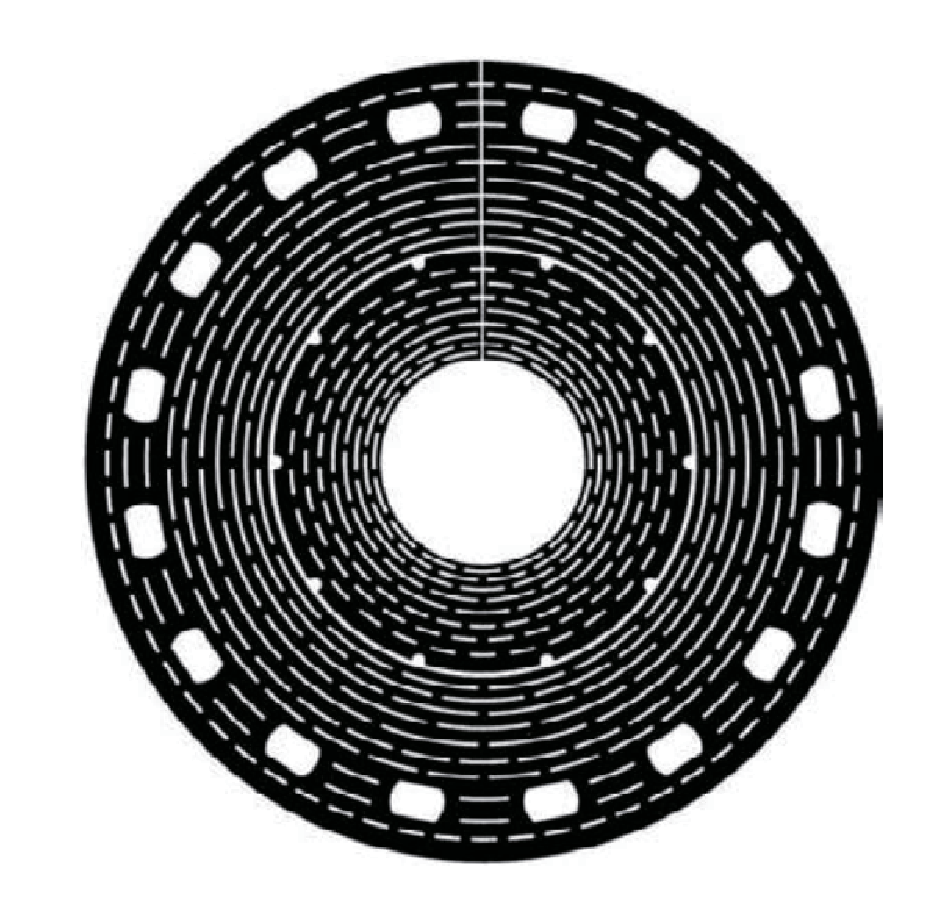
\includegraphics[scale=0.4]{chpt3/figs/fig3.18.eps}
  \caption{国家高场实验室水冷磁体中的两个嵌套``Florida-Bitter''板。外盘直径140\ mm。}
\end{figure}

\textbf{A. 电流密度、场、能量}

本节我们推导Bitter磁体的电流密度$[J_\theta (r)]_B$,中心场$[B_z(0,0)]_B$,场因子$[F(\alpha,\beta)]_B$和G因子$[G(\alpha,\beta)]_B$的表达式。

\textbf{电流密度分布}

考虑一个单盘,电流在$\theta$向流动。电场$E$给出的电压$V$正比于$\theta$。
因为$\vec{E}$仅有$\theta$分量,且在给定$r$处为常量,$E_\theta 2\pi r=V$。
即,$E_\theta$按照$1/r$变化。由于$\vec{J}=\vec{E}/\rho_{Cu}$,有:
\begin{equation}
{[J_\theta(r)]}_B=\frac{E_{\theta}}{\rho_{cu}}=\frac{V}{2\pi\rho_{cu}r}=J_0\frac{a_1}{r}%page123
\end{equation}
式中,$J_0=[J_\theta(a_1)]_B=V/(2\pi \rho_{Cu} a_1)$。
式3.114表明,Bitter磁体中的电流密度按照$1/r$减小,在$r=a_1$处取最大值。

\textbf{场}

我们用式3.114给出的$J_\theta$替换3.107式中的$\lambda J$,在合适的上下限下积分得:
\begin{equation*}
{[B_z(0,0)]}_B=\mu_0\lambda_B J_0a_1\int_{a_1}^{a_2}\int_{0}^{b}\frac{r dr dz}{{r^2+z^2}^{3/2}}
=\mu_0\lambda_B J_0 a_1\int_{1}^{\alpha}\int_{0}^{\beta}\frac{\eta d\eta d\zeta}{{\eta^2+\zeta^2}^{3/2}}%page123
\end{equation*}
式中,$r/a_1=\eta$,$z/a_1=\zeta$。查积分表,得到:
\begin{equation*}
\int_{0}^{\beta}\frac{d\zeta}{{\eta^2+\zeta^2}^{3/2}}=\left[\frac{\zeta}{\eta^2\sqrt{\eta^2+\zeta^2}}\right]_0^{\beta}=\frac{\beta}{\eta^2\sqrt{\eta^2+\beta^2}}%page123
\end{equation*}

联立上面两式,得:
\begin{equation*}
\begin{split}
{[B_z(0,0)]}_B&=\mu_0\lambda_B J_0a_1\beta\int_{1}^{\alpha}\frac{\eta d\eta}{\eta^2\sqrt{\eta^2+\beta^2}}\\
&=\mu_0\lambda_B J_0a_1\beta\left[-\frac{1}{\beta}\ln\left(\frac{\beta+\sqrt{\beta^2+\eta^2}}{\eta}\right)\right]_1^{\alpha}\\ %page123
&=\mu_0\lambda_B J_0a_1\ln\left(\alpha\frac{\beta+\sqrt{1+\beta^2}}{\beta+\sqrt{\alpha^2+\beta^2}}\right)%page123
\end{split}
\end{equation*}

上面的表达式还可写为:
\begin{subequations}
	\begin{align}
{[B_z(0,0)]}_B=&\mu_0\lambda_B J_0a_1[F(\alpha,\beta)]_B\\ %page123
{[F(\alpha,\beta)]}_B=&\ln\left(\alpha\frac{\beta+\sqrt{1+\beta^2}}{\beta+\sqrt{\alpha^2+\beta^2}}\right)%page123
	\end{align}
\end{subequations}

注意3.115b和3.15b两式的区别。

\textbf{场和能量}

我们通过在整个线圈区域内对功率密度$\rho_{Cu} [J_\theta]_B^2(r)$积分导出$[H_z(0,0)]_B$和Bitter磁体总功率$P_B$的关系式。这里继续采用无量纲参数,有:
\begin{equation*}
P_B=a_1^3\int_{1}^{\alpha}\int_{-\beta}^{\beta}\rho_{cu}\lambda_B\left(\frac{J_0}{\eta}\right)^2 2\pi\eta d\zeta d\eta=J_0^2\rho_{cu}\lambda_B a_1^3(4\pi\beta\ln\alpha)%page124
\end{equation*}

通过上式,我们将$J_0$和$P_B$联系起来:
\begin{equation*}
J_0=\frac{1}{a_1\sqrt{4\pi\beta\ln\alpha}}\sqrt{\frac{P_B}{\rho_{cu}\lambda_B a_1}}%page124
\end{equation*}

将上式和式3.115联立,将$[B_z(0,0)]_B$和$P_B$联系起来:
\begin{subequations}
	\begin{align}
{[B_z(0,0)]}_B&=\mu_0[G(\alpha,\beta)]_B\sqrt{\frac{\lambda_B P_B}{\rho_{cu}a_1}}\\%page124
{[G(\alpha,\beta)]}_B&=\frac{1}{\sqrt{4\pi\beta\ln\alpha}}[F(\alpha,\beta)]_B%page124
	\end{align}
\end{subequations}

在均匀电流密度螺管线圈中,$[B_z(0,0)]_B$按$P_B$的平方根增加;$P_B$是磁场的二次函数。
$[G(\alpha,\beta)]_B$在$\alpha\simeq 6.42$和$\beta\simeq 2.5$时取得最大值,此时$[G(6.4,2.15)]_B\simeq 0.166$。在$5\leq \alpha \leq 9$和$1.8\leq\beta\leq 2.6$范围内,$[G(\alpha,\beta)]_B$的值
至少是其峰值的99\%。也就是说,在这个$\alpha$和$\beta$范围内,在给定场下,$P_B$的变动最小值为2\%以内。
不过,给定$a_1$时,场的均匀性随$2b$或$\beta$增大而改善。故大多数Bitter磁体的$\beta>2.5$,
就如下面给出的这个磁体一样。

\textbf{实例}\quad 我们式3.116计算一个Bitter磁体的$P_B$。
磁体参数:$2a_1=6\ \mathrm{cm}, 2a_2=40\ \mathrm{cm}, 2b=22 \ \mathrm{cm},\lambda_B=0.8$以及$\rho_{Cu}=2\times 10^{-6}\ \Omega\mathrm{cm}$,
产生磁场$[B_z(0,0)]_B=20\ \mathrm{T}$。
代入参数$\alpha=a_2/a_1=40/6=6.67;\beta=b/a_1=22/6=3.67$,
\begin{equation*}
{[G(6.67,3.67)]}_B=\frac{1}{\sqrt{4\pi3.67\ln(6.67)}}\ln\left[6.67\frac{3.67+\sqrt{1+(3.67)^2}}{3.67+\sqrt{(6.67)^2+(3.67)^2}}\right]\simeq 0.159 %page124
\end{equation*}

类似式3.113c,可以将$P_B$写成$[B_z(0,0)]_B$和其他参数的表达式:
\begin{align*}
P_B&=\frac{\rho_{cu}a_1[B_z(0.0)]_B^2}{\mu_0^2\lambda_B[G(\alpha,\beta)]_B^2}=\frac{(2\times 10^{-8}\ \Omega\mathrm{m})(3\times 10^{-2}\ \mathrm{m})(20\ \mathrm{T})^2}{(4\pi\times 10^{-7}\ \mathrm{H/m})^2(0.8)(0.159)^2}\\
&\simeq 7.5\ \mathrm{MW}%page124
\end{align*}

这个功率是运行于Francis Bitter国家磁体实验室的$20\ \mathrm{T}$Bitter磁体的典型值。

\textbf{B. 非``Bitter"型电流密度分布}

水冷磁体的一个重要参数是磁场效率,定义为:$[B_z(0,0)]_B^2/\mu_0^2 P_B$。
作为均匀电流密度磁体,Bitter磁体的磁场效率正比于$\lambda_B$和$[G(\alpha,\beta)]_B^2$,
反比于$a_1$和导体电阻率$\rho_{Cu}$。

我们目前考虑了两种电流分布:1) 均匀型,即$J(r,z)=J_0$;2) Bitter型,即$J\propto 1/r$。
均匀分布意味着$J$与$r$和$z$无关。
由``分级''超导材料绕的超导磁体的$J(r)$随$r$离散阶梯变化。
由多个嵌套线圈组成的磁体,若各线圈由不同的超导材料绕制,其$J(r)$同样随$r$阶梯变化。
这里我们介绍另外三种用于水冷磁体的电流分布。

\textbf{Kelvin线圈}

具有最高磁场效率的电流密度分布被称为Kelvin分布:
\begin{equation*}
J_K(r,z)\propto\frac{r}{(r^2+z^2)^\frac{3}{2}}%page125
\end{equation*}

Kelvin线圈的独有性质是每个部分的单位功率都产生相同的磁场。
作为对比,总功率相同的均匀电流密度线圈产生的磁场是磁体中心场的66\%;
而Bitter线圈的这个比值是77\%。
不过,制成具有Kelvin电流分布的线圈并不具可行性。

\textbf{Gaume}

Gaume分布同样给出很好的磁场效率:
\begin{equation*}
J_G(r,z)\propto\frac{1}{r}\left(\frac{1}{\sqrt{a_1^2+z^2}}-\frac{1}{\sqrt{a_2^2+z^2}}\right)%page125
\end{equation*}

Gaume线圈的每一匝在单位功率下产生相同的磁场。
Gaume线圈产生的磁场是Kelvin线圈的85\%。
Bitter线圈的电流分布在某种程度上是近似于Gaume线圈的。
这可以通过使用轴向远离磁体中心平面的更厚的Bitter板实现:
$J_b(r,z)\propto 1/r\delta(z)$,此处$\delta(z)$是依赖于$z$的板厚度。

\textbf{多螺旋}

多螺旋线圈由多个嵌套的单层线圈组成,
每一层的电流密度经调整,具有最大化磁场效率并/或匹配每一层导体应力的能力:
\begin{equation*}
J_P(r,z)\propto f(r)%page125
\end{equation*}

最高效率的多螺旋线圈,其$J_P(r,z)\propto 1/r^2$,可以产生92\%的Kelvin磁场。
实践中,多螺旋线圈由于两端需要很多电极,而被认为比Bitter线圈更难于制造。


\subsection{问题3.2:螺管中的最大场}
磁体中心轴向场是用户通常明确的重要参数,
对磁体设计者来说同等重要的另一个参数是磁体的最大场。
在单螺管磁体中,如时3.12b给出的,中平面轴向场$H_z(r,\theta)$在室温孔内沿径向增加。
实际上,轴向的最大场出现在中平面上最内层绕组的半径点:$H_m=H_z(a_1,0)$。
在由多个嵌套线圈组成的多线圈磁体中,最大场却肯定不在最内层线圈上,而是偏离$(a_1,0)$点的。
这是由于其余线圈产生的场通常并非轴向。

再次说明,对本主题只是为了增进读者对简单螺管线圈场分布的理解。
在实际的多线圈磁体中,只能根据程序来计算各线圈的最大场及其出现位置。

a) 使用3.4节中的表达式,证明对``薄壁"线圈($\alpha=1$),有关系式$H_z(r,0)/H_z(0,0)=h_z(\xi)$,其中$\xi=r/a_1$:
\begin{align}
h_z(\xi)=1&+\frac{3}{4(1+\beta^2)^2}\xi^2+\frac{15(3-4\beta^2)}{64(1+\beta^2)^4}\xi^4+\frac{35(5-20\beta^2+8\beta^4)}{256(1+\beta^2)^6}\xi^6\\\notag
&+\frac{315(35-280\beta^2+336\beta^4-64\beta^6)}{16384(1+\beta^2)^8}\xi^8\\\notag
&+\frac{693(63-840\beta^2+2016\beta^4-1152\beta^6+128\beta^8)}{65536(1+\beta^2)^{10}}\xi^{10}%page126
\end{align}

b) 证明:对``短"线圈($\beta=0$),$h_z(\xi)$的表达式为:
\begin{align*}
h_z(\xi)=1&+\frac{3(\alpha^2-1)}{8\alpha^2\ln\alpha^2}\xi^2+\frac{45(\alpha^4-1)}{256\alpha^4\ln\alpha}\xi^4+\frac{175(\alpha^6-1)}{1536\alpha^6\ln\alpha}\xi^6\\\notag
&+\frac{11025(\alpha^8-1)}{131027\alpha^8\ln\alpha}\xi^8+\frac{43659(\alpha^{10}-1)}{655360\alpha\ln\alpha}\xi^{10}\cdots \tag{3.117b}
\end{align*}

c) 类似的,证明:对``薄壁且长"线圈,$h_z(\xi)$为:
\begin{equation*}
h_z(\xi)\simeq 1+\frac{3}{4\beta^4}\xi^2-\frac{15}{16\beta^6}\xi^4+\frac{35}{32\beta^8}\xi^6-\frac{315}{256\beta^{10}}\xi^8+\frac{693}{512\beta^{12}}\xi^{10}-\cdots\tag{3.117c}%page126
\end{equation*}

d) 对``薄壁"线圈($\alpha=1$)和相对短线圈($\beta=0.4$)计算$H_m/H_z(0, 0)\equiv h_m$的\textit{近似}值。

e) 计算饼式线圈($\alpha=2,\beta\simeq 0$)的$h_m$。

f) 确定``薄壁"且``长"线圈($\alpha=1,\beta=2$)的$h_m$。 

注对任意$\alpha,\beta$组合的单螺管线圈,$H_m/H_z(0,0)$可由式3.12b和3.14中的$h_z(\xi)$给出。

\subsubsection{问题3.2之解}
a) 考虑到$H_z(r,0)$在中平面上与$H_z(x, 0)$或$H_z(y, 0)$等价,我们使用式3.12b,其中$\xi = x/a_1$,$\xi = y/a_1$或$\xi = r/a_1$。对于``薄壁"螺管,我们可以通过联立3.12b和3.25得到3.117a。

b) 类似的,3.117b可以通过联立3.12b和3.21得到。

c) 通过联立3.12b和3.26得到3.117c。
和3.117b中的高阶项的符号都是正的不同,3.117c中的项是正负交替的。 

d) 将$\beta=0.4,\xi=1$代入3.117a,得:
$$h_m=1 + 0.5574 + 0.3055 + 0.1125 − 0.0086 − 0.0585 = 1.9082$$
在Montgomery给出的$\beta$和$F(\alpha,\beta)$为定值时的$H_m/H_z(0,0)$ vs. $\alpha$图中[3.2],
给出的值为1.87。

e) 将$\alpha=2,\xi=1$代入3.117b,得:
$$ h_m\simeq 1 + 0.4058 + 0.2378 + 0.1618 + 0.1209 + 0.0960 = 2.0222$$

f) 将$\beta=2,\xi=1$代入3.117a,得:
$$ h_m\simeq 1 + 0.03 − 0.0049 + 0.0005 + 0.0000 − 0.0000 = 1.0256 $$

一个更快但稍不精确的解可由3.117c得到,该式事实上只在$\beta\gg 1$时成立:
$$h_m \simeq 1 + 0.0469 − 0.0146 + 0.0043 − 0.0012 + 0.0003 = 1.0356$$



\subsection{讨论3.3:负荷线}
\textbf{A. 用``各向同性"超导体绕成的螺管线圈磁体}

图3.19给出了``各向同性''超导体在给定温度$T_0$下临界电流$I_c$与$B$的关系$I_c(B,T_0)$
以及超导螺管磁体的两组``负荷线"。
这里,$I_c(B,T_0)$曲线是各向同性的,即与场方向无关。通常圆截面超导体的特性能满足这个条件。

从对应``自场"的$B_z(0,0)$开始的实线和虚线负荷线分别为表示轴向场$B_z(0,0)$和绕组内的最大场$B_{mx}$
---对简单螺管磁体,$B_{mx}$出现在绕组内半径($r=a_1$)和轴向中平面($z=0$)处,$B_{mx}=B_z(a_1,0)$。
$I_c(B,T_0)线$和虚线负载线交点是磁体可以保持全超导态的允许最大运行电流,$I_{op}(B_{mx},T_0)$。

当磁体置于另一个磁体的室温孔中,``背景场''磁体产生的场必须附加加到内磁体的负载线上,
即所谓的``内插"---在一个组合磁体系统中,两个磁体一般是同轴且中平面重合的。
在$B$轴上以$B_{bo}$为起点的实线表示组合系统的中心场,虚线表示对应最大内插场
---注意到虚线起点略高于$B_{bo}$,因为那里的背景场更大;
$I_c(B,T_0)$线和虚线的交点给出了这个组合磁体的最大运行电流$I_{op}(B_{mxb},T_0)$。

出于各种原因,后面各章节讨论的一些不论是孤立的还是组合的超导磁体,
通常其设计运行电流为其允许最大电流的50–70\%。

\begin{figure}[htbp]
	\centering
	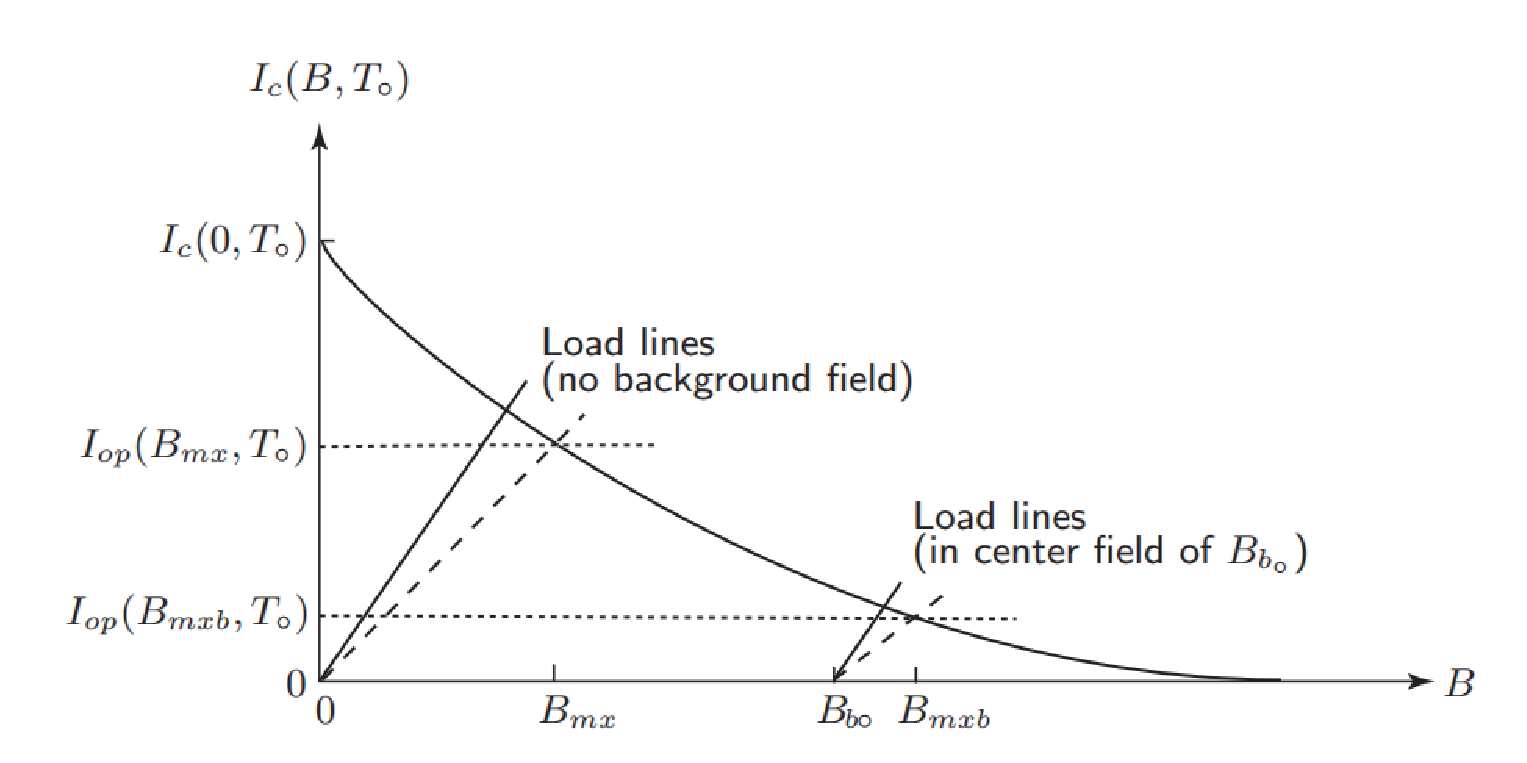
\includegraphics[scale=0.5]{chpt3/figs/fig3.19.eps}
	\caption{``各向同性''超导体在给定温度$T_0$下临界电流$I_c$与$B$的关系曲线;螺管磁体的两组``负荷线"---自场以及置于一个产生背景中心场为$B_{b0}$的螺管磁体室温孔中两种情况。}
\end{figure}

\textbf{B. 用``各向异性''超导体绕制的螺管线圈磁体}

对于非圆截面超导体,$I_c(B,T_0)$通常是``各向异性"的,即$I_c(B,T_0)$依赖于磁场相对于截面的方向。
非圆截面超导体的典型例子就是高温超导体Bi2223和YBCO,他们仅能做成``带"的形式。

附录V中给出了Bi2223和YBCO的$I_c(B, T)/I_c(sf,77\ \mathrm{K})$图---$I_c(B, T)$数据归一化为$I_c(sf,77\ \mathrm{K})$数据。其中的sf表示``自场"(self field),即传导电流自身产生的磁场。
每一种超导体都给出了两组数据,一组是外施磁场平行于超导体的``宽"面($B_{\parallel}$),
一组是外施磁场垂直于超导体``宽"面($B_{\perp}$)。 
Bi2223和YBCO的$I_c(B,T_0)$都是在$B_{\perp}$中下降更快。
另一个值得注意的是,两种超导体的临界电流$I_c(B)$在两种方向的磁场下都是磁场越大下降越快。

从图3.3所示的螺管磁体的场线可以推断出,
磁场径向分量$B_r$在螺管轴向中平面($z=0$)上严格为零,
在$\pm b$和$r$方向随坐标增加,在$z=\pm b,a_1 < r < a_2$存在最大径向场$[B_r(\alpha,\beta)]_{pk}$。
尽管并不存在$[B_r(\alpha,\beta)]_{pk}$的闭式解析解。
不过,对于多数单螺管线圈($1\le \alpha \le 3.6 , 0.1\le \beta \le 10$),
在基于带材的磁体初设阶段,例如``双饼''线圈堆叠磁体(讨论3.6),
下面3.118给出的$[B_{r}(\alpha,\beta)]_{pk}$与程序计算结果相差$\pm 30\%$:
\begin{equation}
 \frac{[B_{r}(\alpha,\beta)]_{pk}}{B_{z}(0,0)}\simeq\frac{0.3}{\alpha^{2}\beta}+\frac{0.6}{\alpha}\\%(3.118)
\end{equation}

注意到,对一个``薄壁"或``中等壁厚" ($\alpha \le 1.8$) 且``短" ($\beta < 1$) 的螺管线圈,
$[B_r(\alpha,\beta)]_{pk}$ 可能\textit{超过}$B_z(0, 0)$,例如$[B_r(\alpha=1.1,\beta=0.1)]_{pk}\approx 3B_z(0,0)$!

所以,带材绕制的磁体的负荷线交点对应最大垂直场$B_{\perp}$,即$[B_r(\alpha,\beta)]_{pk}$。
限制带材运行电流的是带材的$I_c(B_{\perp},T_0)$曲线而不是对应$I_c(B_\parallel, T_0)$的最大$B_\parallel(=B_z)$负荷线。
同时,由于$B_{\perp}$随绕组中带材的高度(带材宽度)变化,
这个变化在计算最大运行电流时也必须予以考虑。
Voccio最近给出了确定Bi2223和YBCO带材绕制的``饼式线圈"最大运行电流的解析方法[3.10]。



\subsection{讨论3.4:叠加技术}
用于求解磁场问题的Biot-Savart定律从根本上阐明了螺管上某点的磁场是螺管上所有电流元在该处
产生的磁场的矢量和(叠加)。
本节我们在整个螺管上应用叠加技术以计算螺管轴线上任一点的磁场。
叠加技术虽仅限于轴线上的磁场,但亦能增进读者对螺管磁场的一般理解。

\textbf{A. 末端场}

轴对称螺管的轴线末端处的磁场是一个结构\textit{等同}但长度加倍的螺管的\textit{中心场}的一半。
我们可以形象的理解:考虑一个由两个完全相同部分组成的轴对称螺管,每个螺管长$2b$(图3.20)。
新螺管的轴向中心场是由两个部分螺管产生的磁场之和:
\begin{equation}
H(b)=H(\alpha,\beta)|_{z=b}=\frac{1}{2}H(\alpha,2\beta)|_{z=0}=\frac{1}{2}\lambda Ja_{1}[F(\alpha,2\beta)]\\%(3.119)
\end{equation}

由于$F(\alpha, 2\beta)>F(\alpha,\beta)$ (图3.17b),自然有$H(z=b)>0.5H(0)$。
也即,单螺管的轴线末端场总是略大于中心场的一半。
在极限$\beta\rightarrow\infty$下,有$H(z=b)\rightarrow 0.5H(0)$。

\textbf{B. 非中点轴向场}

叠加技术还可以用于计算螺管轴线上任一点的轴向场。
这里考虑两个非中点轴向场的实例:1) $0<z<b$,即位于螺管室温孔内;2) $z > b$,即位于螺管室温孔外。
图3.21给出了各实例应用叠加技术的过程。
于是,我们有:
\begin{subequations}
	\begin{align}
&(\mbox{情况1:}z<b)\quad H(z)=\frac{1}{2}\lambda J\alpha_{1}\left[F\left(\alpha,\beta=\frac{b+z}{a_{1}}\right)+F\left(\alpha,\beta=\frac{b-z}{a_{1}}\right)\right]\\%(3.120a)
&(\mbox{情况2:}:z>b)\quad H(z)=\frac{1}{2}\lambda Ja_{1}\left[F\left(\alpha,\beta=\frac{b+z}{a_{1}}\right)-F\left(\alpha,\beta=\frac{z-b}{a_{1}}\right)\right]%(3.120b)
	\end{align}
\end{subequations}

\begin{figure}[htbp]
	\centering
	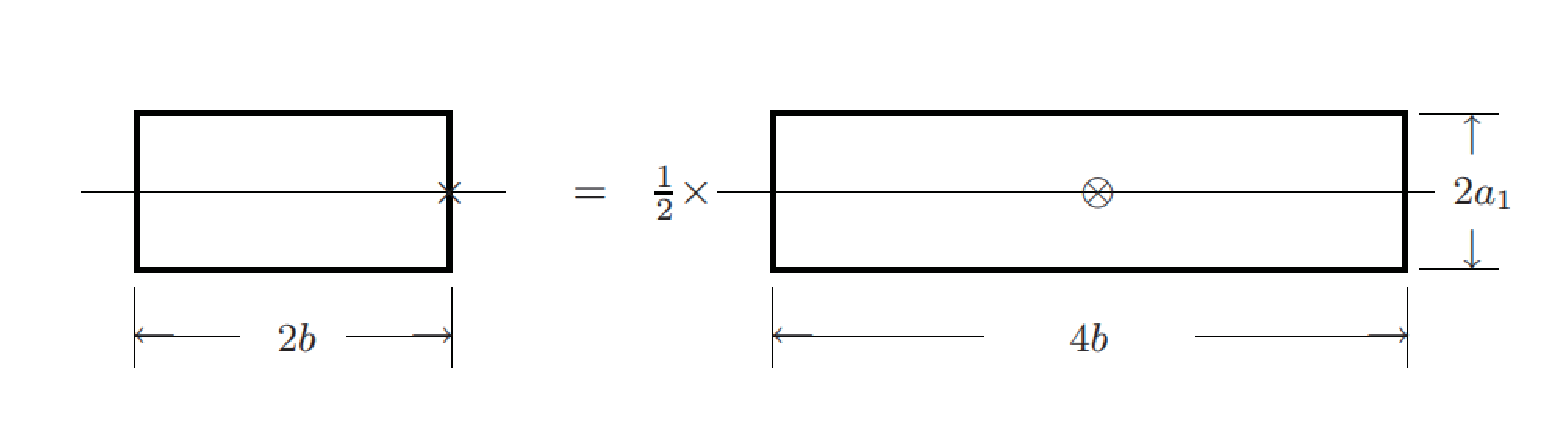
\includegraphics[scale=0.5]{chpt3/figs/fig3.20.eps}
	\caption{采用叠加技术,一个长度为$2b$的轴对称螺管末端磁场可以按照同样结构但长度为$4b$的螺管的中心场的一半计算。}
\end{figure}

\begin{figure}[htbp]
	\centering
	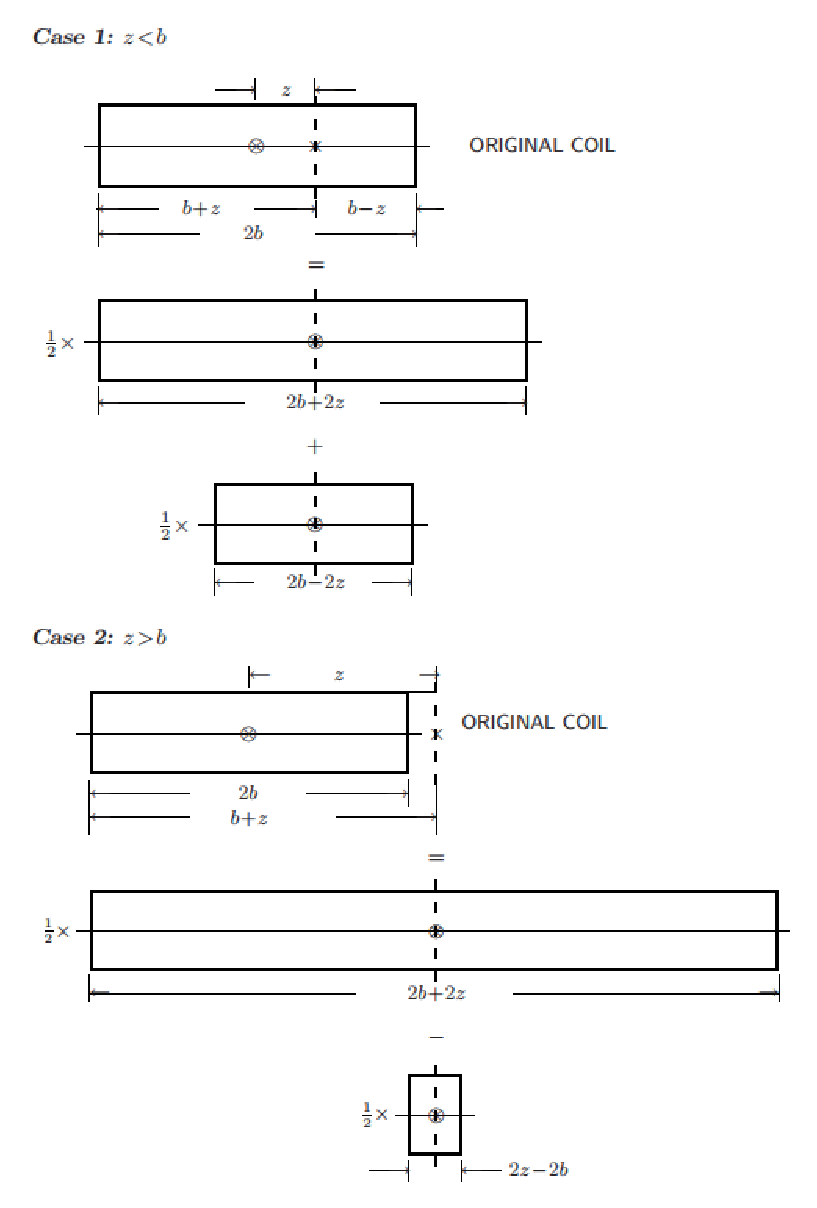
\includegraphics[scale=0.9]{chpt3/figs/fig3.21.eps}
	\caption{计算轴向场任意点磁场的叠加技术。情况1:$z<b$;情况2:$z>b$。}
\end{figure}



\subsection{讨论3.5:混合磁体}
``混合''磁体包括两个轴向对齐且居中但不同种类的电磁体:一个是大功率水冷磁体,一个是超导磁体。
水冷磁体安装在超导磁体室温孔内。
1960年代中期,国家磁体实验室(NML)的Montgomery等人证实,
混合磁体是获得高于$\sim 25\ \mathrm{T}$直流磁场的一种方法[3.11]。
该磁场是当时电源($9\ \mathrm{MW}$)所能支持Bitter磁体实现的最高直流场。
此后30年,磁体实验室设计、制造和运行了多台混合磁体,发展了混合磁体技术[3.12–3.18]。

\textbf{A. 有代表性的混合磁体}

现在有很多个混合磁体在运行。下面以其投入运行的时间为序,对几个有代表性的混合磁体作简要介绍。

\textbf{\kaishu Radboud大学高场磁体实验室}

位于Nijmegen的高场磁体实验室(High Field Magnet Laboratory,HFML)自1977年起,
先后运行了25.4 T[3.12]和32 T[3.14, 3.15]的混合磁体,由6 MW电源供电[3.19]。
他们最近安装了20 MW电源[3.20]并升级了水冷磁体[3.21]。
预计2012年,45 T混合磁体将投入运行。

\textbf{\kaishu Tohoku大学高场实验室}

高场实验室(High Field Laboratory)使用7.5 MW电源,自1983年开始运行23 T混合磁体;
将``湿"混合磁体替换为``干"式后,产生了30 T的磁场[3.23]。

实用化混合磁体应可以经受多次磁场系列过程,其理想的超导磁体应当是\textit{干式}的和\textit{高温超导}的:
干式低温容器可在系列过程中避免其水冷磁体中的液态制冷剂损耗;
高温超导磁体相比低温超导磁体,可以承受由交流损耗引起的更大的温升。
第4章将讨论混合磁体实用化运行条件下,两种甚至可令\textit{干式}高温超导磁体都能可靠运行的设计/运行方式:
1) 超导磁体腔内放置大量固体制冷工质;
2) 采用低温循环器(cryocirculator, 见讨论4.7)而不是制冷机作为超导磁体的初级冷源。

\textbf{\kaishu Grenoble高场实验室}

Grenoble磁体实验室在1987年开始运行混合磁体[3.24]。
他们最近的24 MW电源[3.25]为40 T混合磁体运行提供了条件[3.26]。

\textbf{\kaishu 国家材料科学研究院磁体实验室}

位于Tsukuba的国家材料科学研究院的磁体实验室(Magnet Laboratory at the National Institute of Materials Science)自1995年开始运行混合磁体。他们有一台17 MW电源,用于运行30-35 T混合磁体[3.27]。

\textbf{\kaishu 国家高场实验室(NHMFL)}

Florida州立大学的国家强磁场实验室的45 T混合磁体[3.28, 3.29]产生了世界上最大的直流磁场。
其中,水冷磁体产生磁场34 T,超导磁体产生磁场11 T [3.30]。该超导磁体下文会详细讨论。

\textbf{B. NHMFL 45 T混合磁体}
\begin{figure}[htbp]
	\centering
	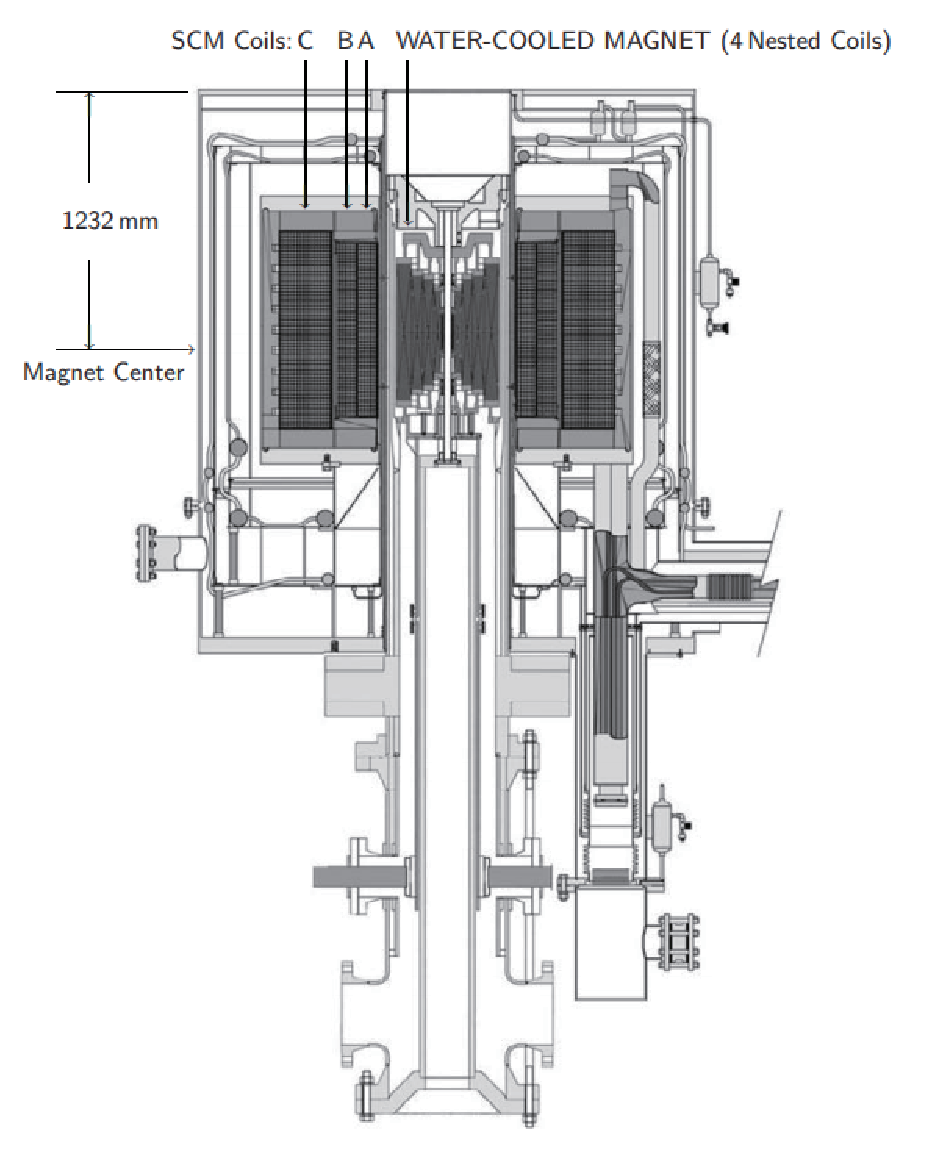
\includegraphics[scale=0.8]{chpt3/figs/fig3.22.eps}
	\caption{NHMFL的45 T混合磁体剖面图。}
\end{figure}

图3.22给出了NHMFL的45 T混合磁体的水冷磁体、超导磁体和一些附件的剖面图[3.31。
水冷磁体有四个嵌套线圈组成,在24 MW功率下产生31 T的中心场。
超导磁体由A、B、C三个线圈组成,运行于1.8 K,最初产生14 T磁场,但现在可产生11 T[3.30];
水冷磁体经重新设计,可以在30 MW功率下产生34 T的磁场。
磁体系统包括超流液氦补给低温容器,超导磁体低温容器通过管道与之相连,见图的中部右侧。

\begin{table}[htbp]\small
\centering
\caption{NHMFL的45 T混合磁体的14 T超导磁体参数[3.31]}
\begin{threeparttable}
\begin{tabular}{|l|c|c|c|}
\hline
线圈(均以CIC导体绕成) & 线圈A & 线圈B & 线圈C \\ \hline
超导材料 & \multicolumn{2}{c|}{$\mathrm{Nb_3Sn}$} & NbTi \\ \hline
绕组类型 & \multicolumn{2}{c|}{层绕} & 饼式 \\ \hline
层数/双饼数 & 6 & 7 & 29 \\ \hline
总匝数 & 306 & 378 & 1015 \\ \hline
绕组内径i.d.,2$a_1$ {[}mm{]} & 710 & 908 & 1150 \\ 
绕组外径o.d.,2$a_2$ {[}mm{]} & 888 & 1115 & 1680 \\
绕组长度, 2b {[}mm{]} & 869 & 868 & 992 \\ \hline
运行电流,$I_{op}$ {[}kA{]} & \multicolumn{3}{c|}{$10^*$} \\ \hline
$\lambda J@I_{op} [\mathrm{MA/m^2}]$ & $39.6^*$ & $44.3^*$ & $38.6^*$ \\ \hline
贡献中心场 @$I_{op}$ {[}T{]} & $3.3^*$ & $3.6^*$ & $7.4^*$ \\ \hline
水冷磁体空载时$B_{peak}$ @$I_{op}${[}T{]} & $15.7^*$ & $11.7^*$ & $8.5^*$ \\ \hline
组合电感{[}H{]} & \multicolumn{3}{c|}{1.96} \\ \hline
储能量 @$I_{op}$ {[}MJ{]} & \multicolumn{3}{l|}{$98^*$} \\ \hline
	\end{tabular}
\begin{tablenotes}
        \footnotesize
        \item[*] 对应运行电流10 kA;现在实际运行于8 kA[3.30]。 %此处加入注释*信息
      \end{tablenotes}
\end{threeparttable}
\end{table}

\textbf{\kaishu 45 T 混合超导磁体参数}

表3.3给出了45T混合超导磁体的关键参数[3.31]。
该超导磁体最突出的特征是它的三个线圈,
每一个都是由CIC(cable-in-conduit)导体绕成的,CIC的更多细节将在第6章讨论。
两个内侧线圈A和B是层绕的,外侧的线圈C是由29个双饼线圈堆叠的。

\textbf{C. 混合磁体的工程挑战}

混合磁体很少,仅在大概五六个重点国家实验室有运行。
混合磁体不是一类采用常规方法制造的,也不是一种可以由一群工程师或物理学家在几个月就能造出的。
因为这种稀缺性,仅有很少的工程师实际参与到设计、制造和运行混合磁体中去。
此外,混合磁体将一个运行于常温一个运行于液氦的两类磁体在空间上紧密结合起来,
两者在电磁和机械上存在强耦合。
于是,混合磁体不仅有针对具体磁体的特定工程问题,还存在特有且重大的设计和运行挑战:处理
低温的超导磁体对室温的磁体机械结构的巨大作用力并最小化传入超导磁体低温容器的热负荷。
尽管本书读者的大部分根本不会碰到混合磁体,
但它为磁体和低温工程师提供了有指导意义的设计和运行要点。

关于混合磁体的一般话题在本节后面和第4、6、7、8章都会涉及,
这些话题都是基于MIT一致运行到1995年的35 T混合磁体的[3.16–3.18]。

\textbf{D. 配置和独有特征}

混合磁体中,超导磁体\textit{总}是置于水冷磁体(``内插'')的外侧。
在这种配置下,每一组件的特性如下进行优化。

\textbf{水冷磁体}
\begin{itemize}
	\item 在讨论3.2中已经证明,Bitter磁体的功率需求$P_B$正比于$a_1$和$[B_z(0, 0)]^2_B$ (3.116a),
	其中,$P_B$典型值为$6\sim 30\ \mathrm{MW}$。Bitter磁体相当耗电,故最好对其进行总体优化:
	作为混合磁体的内插单元。
	然而,磁场越强,磁场对导体的磁应力越大,导体材料强度就该越强,而这一般意味着更大电阻。
	于是,$B_z(0, 0)\propto\sqrt{P}$ (3.113a)和$[B_z(0, 0)]_B\propto\sqrt{P_B}$ (3.116a)在高场时
	都不再有效。
	\item 常规金属(比如铜)没有``固有"的磁场极限,即不存在高于某个场就不能用它制造磁体的问题。
	但是,如上所述,由于高强度的材料需要更大功率,同时需要更多的冷量以匹配增加的焦耳热。
	$30-40\ \mathrm{T}$一般被认为是可实现磁体的极限。
\end{itemize}

\textbf{超导磁体}
\begin{itemize}
	\item 超导体都有明确的可以保持超导态的上临界场。于是,最好将超导磁体放在混合磁体
	的低场部分:置于水冷磁体外侧。
	
	\item 总的存储磁能随磁体大小增加而增加,但对功率的需求---主要来自制冷---并不显著。
	$100\ \mathrm{MJ}$的磁体并不需要$100\ \mathrm{MW}$的电源;通常$10-100\ \mathrm{kW}$就够了。
\end{itemize}

统筹考虑这些特征,我们就很自然的理解为什么混合磁体的水冷磁体放在内部,超导磁体包在外部了。

\textbf{作用力}

混合磁体的一个独特特征和需求源自内插磁体和超导磁体间相互作用力。
如果两个磁体轴向和径向都是对齐的,它们之间无作用力。
但是,他们场中心的相对错位会导致很大的作用力。
轴向错位产生轴向恢复力---回到到磁体中心轴。
场中心的径向错位将导致错位程度进一步增加,即失稳。
一般的,力大小是适中的;小心的设计和建造可以比较容易的应对此事。
不过,高性能水冷内插磁体的失效是必须认为是不可避免的。
若失效,比如当内插绕组短路时,产生的磁场减小,将会因磁场未对齐突然产生很大的力。

为了控制故障力,结构上的需求是最重要。由于两个磁体的磁耦合(互感),磁体的监控保护变得很复杂。
很明显,每个磁体及其电源系统都必须有自己的某种电保护以防止在哪里出错的时候损伤或损毁,
另外两个磁体间还存在很强的电气耦合。
第8章的问题8.3和问题8.4将讨论磁体线圈的监测的一般问题和针对混合磁体的特定问题。


\subsection{讨论3.6:``双饼'' vs. ``层绕''}
磁体的两种绕制技术一种通常被称为``双饼"或简单的称为``饼",另一种称为``层绕"。
双饼线圈的绕制通常使用扁平导体(如带材),有时也采用``大''的正方或长方形截面的导体(如CIC)。
不管怎么绕,都要使用一根连续的导体。
双饼线圈如图3.23所示,绕制的起点是导体的中点(图中的C附近);
而层绕的话,起点在导体的一端(图中的A或B)。
因为每个双饼线圈的绕组高度$(2b)$大约是导体高度(带材宽度)的2倍,
所以实际磁体需由多个双饼线圈组成,相邻线圈在径向最外侧$(2a_2)$之外连接。
而层绕线圈是从一端到另一端连续绕制,从最里层到最外层一层一层绕成。
两种技术的优缺点下文将加以讨论。

\begin{figure}[htbp]
	\centering
	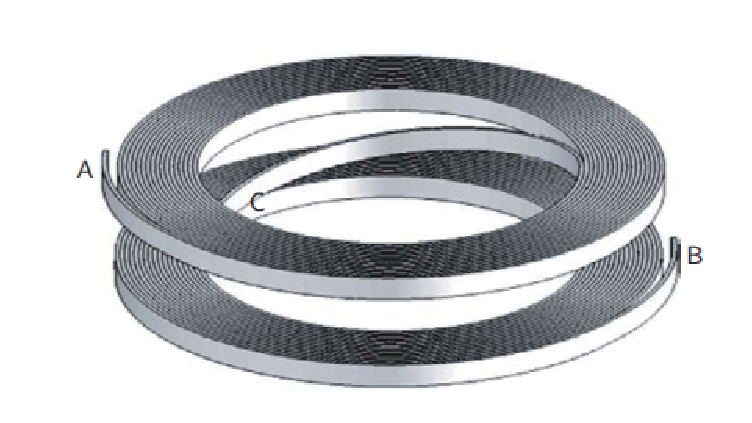
\includegraphics[scale=0.7]{chpt3/figs/fig3.23.eps}
	\caption{双饼线圈图示。为了清晰,上下饼分开了。图中这种双饼是由超导带材绕制的,点A和点B是连续导体的端头,而点C大约是带材的中点。}
\end{figure}

\textbf{优势和劣势}
\begin{enumerate}
	\item 对双饼线圈,对导体长度的要求低于不分段的层绕线圈。导体无接头长度$\sim 50\ \mathrm{m}$
	就够绕一个小线圈了。对大型磁体,$\sim 1-2\ \mathrm{km}$也够了。
	另一方面,对层绕线圈,单个线圈所需的无接头导体长度动不动就会超过$10\ \mathrm{km}$。
	由于长导体更难制造,所以在导体长度要求意义上,饼式线圈优于层绕线圈。

	\item 饼式线圈磁体一般要求很多双饼线圈,理想状态下每个双饼应该是完全一致的模块。
	这种\textit{模块化}制造磁体的方法,结合上面提及的对导体长度要求,
	使饼式线圈磁体的制造更加简单(或许也更便宜)。
	此外,层绕线圈可能出现在绕制过程中一个问题就导致整个线圈的导体都不能用的情况;
	在饼式线圈这里仅影响到一个双饼的导体量。
	由于每个双饼的电磁性能和尺寸会存在微小差异,所以饼式线圈的另一个技术的优点就是
	它可以让各饼沿磁体轴线安装在最适合的位置。

	\item 饼式线圈的一个明显劣势是它不可避免的要进行相邻双饼连接。
	连接为磁体制造增加了一个环节。由于连接必须随依绕组的形状,实施起来要比单一导体焊接困难。
	或许对于运行更重要的是这些接头产生的焦耳热---除非接头也是超导的。
	NMR和MRI磁体一般要求超导接头。做超导接头本身就是很有挑战性的;
	确保各个接头能超导也不是一项容易的任务。
\end{enumerate}



\subsection{问题3.3:Helmholtz线圈}
很多应用都希望有高均匀性的磁场。
一种被称为``Helmholtz coil"的简单布局可以在一个有限的区域内实现高均匀磁场。
它使用两个一样的线圈,在磁场轴线($z$向)分开一定距离同轴放置(图3.24a);
两线圈分别位于$z = d/2$和$z = −d/2$。通过调整间隔$d$,使得磁体中心处于($r=0,z=0$):
%3.121
\begin{equation}% 3.121
\frac{d^2H_z(0,z)}{dz^2}\mid_{z=0}=0
\end{equation}

a) 将两个线圈看成半径为$a$的理想``环"线圈。证明:当$d=a$时,在磁体中心处有$dH^2_z(0, z)/dz^2 = 0$。
图3.24b中的实线给出了一个不满足式3.121的$d$下的某线圈的$H_z(0, z)$。

b) 证明:两个线圈如果反极性,磁体中心会产生一个梯度场
计算$dH_z/dz$在$z=0$的值。(注意,当$d=a$时,$d^3H_z(0,z)/dz^3 \neq 0$;$d^3H_z(0,z)/dz^3=0$要求$d=\sqrt{3}a$) 。
此种通过反向电流的配置称为Maxwell线圈。图3.24b中的虚线给出了梯度线圈的$H_z(z)$。

\begin{figure}[htbp]
	\centering
	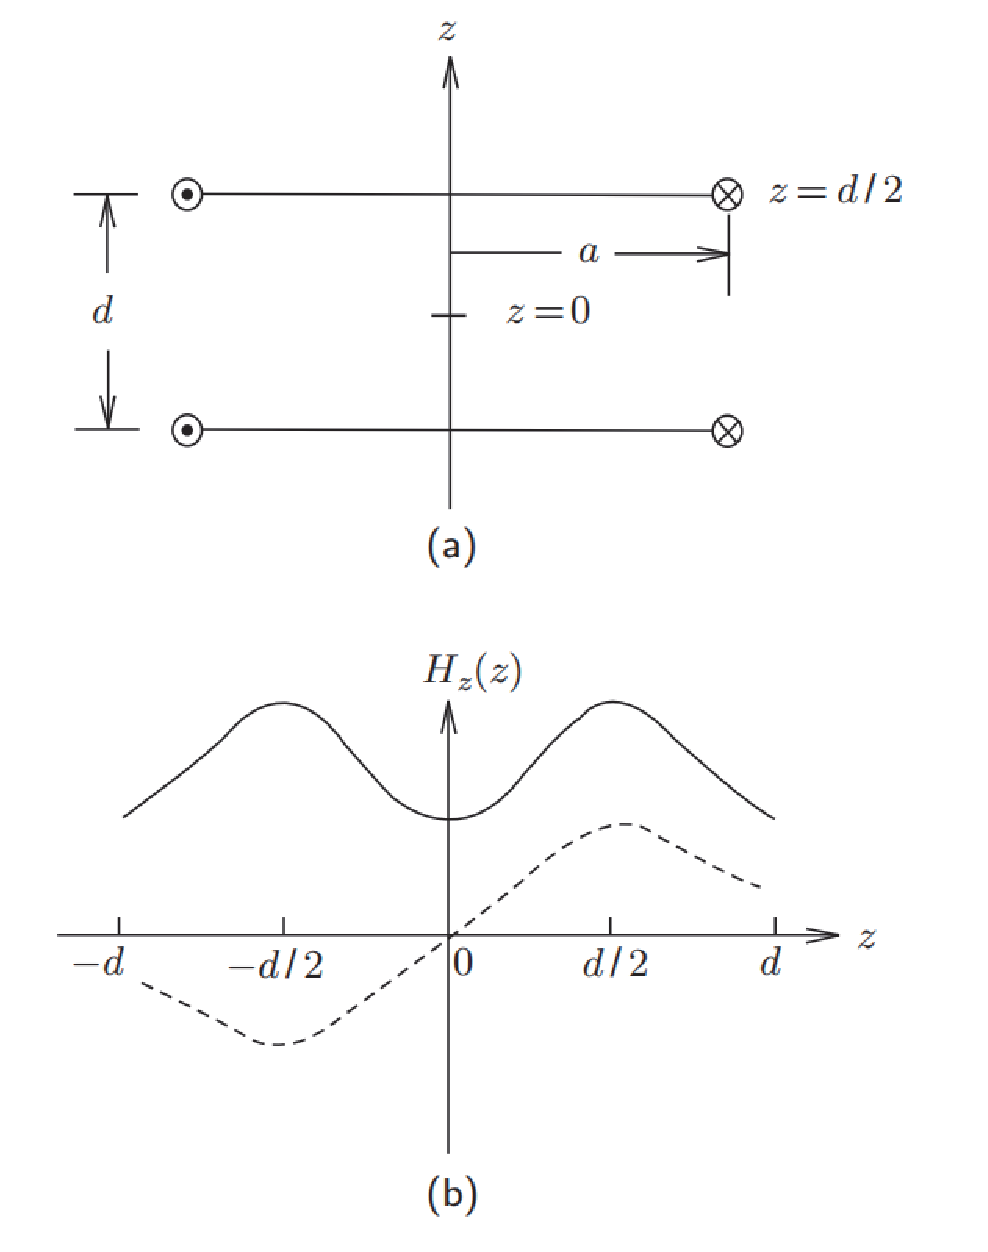
\includegraphics[scale=0.4]{chpt3/figs/fig3.24.eps}
	\caption{(a)理想Helmholtz线圈布局;(b)``均匀''场下的$H_z(0,z)$(实线)和``梯度''场下的$H_z(0,z)$(虚线)。}
\end{figure}

\subsubsection{问题3.3之解}
a) 位于下方$z=−d/2$处的环线圈产生的轴向($r =0$)磁场的$z$分量可由式3.3a给出:
% 方程
\begin{equation*}% page139
H_z(0,z)=\frac{a^2I}{2[a^2+(z+\frac{d}{2})^2]^\frac{3}{2}}
\end{equation*}

加上位于上面$z=d/2$处的环线圈的磁场,有:
%S3.1
\begin{equation*}% S3.1
H_z(0,z)=\frac{a^2I}{2}\left\{\frac{1}{[a^2+(z+\frac{d}{2})^2]^\frac{3}{2}}+\frac{1}{[a^2+(z-\frac{d}{2})^2]^\frac{3}{2}}\right\} \tag{S3.1}
\end{equation*}

将S3.1给出的方程$H_z(z)$对$z$微分,有:
% 方程
\begin{equation*}
\frac{dH_z(0,z)}{dz}=\frac{3a^2I}{2}\left\{{-\frac{(z+\frac{d}{2})}{[a^2+(z+\frac{d}{2})^2]^\frac{5}{2}}-\frac{(z-\frac{d}{2})}{[a^2+(z-\frac{d}{2})^2]^\frac{5}{2}}}\right\}
\end{equation*}

由于对称性,$dH_z(0,z)/dz=0$在$z=0$处对任意$a$成立。

式S3.1的二阶导数为:
% 方程
\begin{equation*}
\frac{d^2H_z(0,z)}{dz^2}=\frac{3a^2I}{2}\left\{{-\frac{a^2-4(z+\frac{d}{2})^2}{[a^2+(z+\frac{d}{2})^2]^\frac{7}{2}}}
-\frac{a^2-4(z-\frac{d}{2})^2}{[a^2+(z-\frac{d}{2})^2]^\frac{7}{2}}\right\}
\end{equation*}

若在$z = 0$处二阶导数为零,应有$d = a$。
这种同轴放置两个一样的线圈且其距离等于线圈半径的技术产生了一个均匀场区域。
这里的二次谐波分析,是MRI和其他要求高空间均匀性磁场磁体设计的重要准则之一。

b) 对该系统,将下方环线圈的电流极性反转,有:
% s3.2
\begin{equation*}% S3.2
H_z(0,z)=\frac{a^2I}{2}\left\{{-\frac{1}{[a^2+(z+\frac{d}{2})^2]^\frac{3}{2}}+\frac{1}{[a^2+(z-\frac{d}{2})^2]^\frac{3}{2}}}\right\} \tag{S3.2}
\end{equation*}

根据对称性,$H_z(z=0)=0$。对S3.2依$z$求导,有:
%s3.3
\begin{equation*}% S3.3
\frac{dH_z(0,z)}{dz}=\frac{3a^2I}{2}\left\{{\frac{(z+\frac{d}{2})}{[a^2+(z+\frac{d}{2})^2]^\frac{5}{2}}-\frac{(z-\frac{d}{2})}{[a^2+(z-\frac{d}{2})^2]^\frac{5}{2}}}\right\} \tag{S3.3}
\end{equation*}

在$z=0$处计算S3.3,有:
%方程
\begin{equation*}
\frac{dH_z(0,z)}{dz}\bigg|_0=\frac{3a^2Id}{2[a^2+(\frac{d}{2})^2]^\frac{5}{2}}
\end{equation*}

这种同轴放置两个一样但电流方向相反的线圈以产生梯度场的方法是对中平面梯度场有要求的磁体的
设计中使用的基本法则。MRI系统中使用脉冲磁体产生梯度场(提取空间信息以成像)就是一个例子。


\subsection{问题3.4:Helmholtz线圈的分析---另一种方法}
这一节,我们使用式3.16a和3.22来分析问题3.3中的Helmholtz线圈。

证明,两个半径为$a$、分别位于$\xi(\equiv z/a)=+0.5$ 和$\xi=−0.5$的``环"线圈1和2组成的Helmholtz对,
轴向场在其中心($\xi=0$)的二阶导数$d^2 h_z(0)/d\xi^2|_{1/2}$可以表示为$\xi^{2n}$的级数且随着
项数增加而收敛于0。由于并未计算各线圈自己在$\xi=0$的值,所以3.17b的简化表达式不能用在这里。

使用至第20阶项计算$d^2 h_z(0)/d\xi^2|_{1/2}$。注意到$E_2(1, 0)\cdots E_{10}(1, 0)$已由3.28给出。
推导$E_2(1, 0)\cdots E_{10}(1, 0)$的技术同样也可用于从3.15b推导出$E_{12}(\alpha, 0)\cdots E_{20}(\alpha, 0)$。$f_{12}(\alpha,\beta)\cdots f_{20}(\alpha,\beta)$在附录IB中有。
在极限$\beta\rightarrow 0$下,将$1/(1+\beta^2)^{19.5}$展开至$\beta^{20}$项,有:
%3.122
\begin{equation}% 3.122
\begin{split}
\frac{1}{(1+\beta)^{19.5}}=1&-\frac{39}{2}\beta^2+\frac{39}{2}\cdot\frac{41}{2}\frac{\beta^4}{2!}-\frac{39}{2}\cdot\frac{41}{2}\cdot\frac{43}{2}\frac{\beta^6}{3!}+\cdots\\
&+\frac{39}{2}\cdot\frac{41}{2}\cdot\frac{43}{2}\cdot\frac{45}{2}\cdot\frac{47}{2}\cdot\frac{49}{2}\cdot\frac{51}{2}\cdot\frac{53}{2}
\cdot\frac{53}{2}\cdot\frac{57}{2}\frac{\beta^{20}}{10!}
\end{split}
\end{equation}

$E_{12}(\alpha, 0)\cdots E_{20}(\alpha, 0)$类似于式3.21中的$E_{2}(\alpha, 0)\cdots E_{10}(\alpha, 0)$,有:
%3.123
\begin{subequations}% 3.123a
	\begin{align}
E_{12}(\alpha,0)&=\frac{7\cdot11\cdot13}{2^{12}}\cdot\frac{(\alpha^{12}-1)}{\alpha^{12}\ln\alpha}=\frac{1001(\alpha^{12}-1)}{4096\alpha^{12}\ln\alpha}\\
E_{14}(\alpha,0)&=-\frac{5\cdot9\cdot11\cdot13}{2^{12}\cdot7}\cdot\frac{(\alpha^{14}-1)}{\alpha^{14}\ln\alpha}=-\frac{6435(\alpha^{14}-1)}{28672\alpha^{14}\ln\alpha}\\
E_{16}(\alpha,0)&=\frac{5\cdot9\cdot11\cdot13\cdot17}{2^{19}}\cdot\frac{(\alpha^{16}-1)}{\alpha^{16}\ln\alpha}=\frac{109395(\alpha^{16}-1)}{524288\alpha^{16}\ln\alpha}\\
E_{18}(\alpha,0)&=-\frac{5\cdot11\cdot13\cdot17\cdot19}{2^{17}\cdot3^2}\cdot\frac{(\alpha^{18}-1)}{\alpha^{18}\ln\alpha}=-\frac{230945(\alpha^{18}-1)}{1179648\alpha^{18}\ln\alpha}\\
E_{20}(\alpha,0)&=\frac{3\cdot7\cdot11\cdot13\cdot17\cdot19}{2^{20}\cdot5}\cdot\frac{(\alpha^{20}-1)}{\alpha^{20}\ln\alpha}=\frac{969969(\alpha^{20}-1)}{5242880\alpha^{20}\ln\alpha}
\end{align}
\end{subequations}

在极限$\alpha\rightarrow 1$时,式3.123a-3.123e成为:
%3.124
\begin{subequations}
	\begin{align}
&E_{12}(1,0)=\frac{3003}{1024}=\frac{3\cdot7\cdot11\cdot13}{2^{10}}=\frac{3\cdot5\cdot7\cdot9\cdot11\cdot13}{2\cdot4\cdot6\cdot8\cdot10\cdot12}\simeq 2.933\\
&E_{14}(1,0)=-\frac{6435}{2048}=-\frac{5\cdot9\cdot11\cdot13}{2^{11}}=-\frac{3\cdot5\cdot7\cdot9\cdot11\cdot13\cdot15}{2\cdot4\cdot6\cdot8\cdot10\cdot12\cdot14}\simeq-3.142\\
&E_{16}(1,0)=\frac{109395}{32768}=\frac{5\cdot9\cdot11\cdot13\cdot17}{10^{15}}=\frac{3\cdot5\cdot7\cdot9\cdot11\cdot13\cdot15\cdot17} {2\cdot4\cdot6\cdot8\cdot10\cdot12\cdot14\cdot16}\simeq 3.338\\
&E_{18}(1,0)=-\frac{230945}{65536}=\frac{5\cdot11\cdot13\cdot17\cdot19}{10^{16}}=-\frac{3\cdot5\cdot7\cdot9\cdot11\cdot13\cdot15\cdot17\cdot19} {2\cdot4\cdot6\cdot8\cdot10\cdot12\cdot14\cdot16\cdot18}\simeq-3.524\\
&E_{20}(1,0)=\frac{969969}{262144}=\frac{3\cdot7\cdot11\cdot13\cdot17\cdot19}{10^{18}}=\frac{3\cdot5\cdot7\cdot9\cdot11\cdot13\cdot15\cdot17\cdot19\cdot21} {2\cdot4\cdot6\cdot8\cdot10\cdot12\cdot14\cdot16\cdot18\cdot20}\simeq 3.700
\end{align}
\end{subequations}

\subsubsection{问题3.4之解}
位于$\xi=+0.5$的线圈1贡献的$d^2h_z(\xi)/d\xi^2$在$\xi=0$时为$d^2h_z(0)/d\xi^2|_{1/2}$,
可由式3.16a给出:
%s4.1
\begin{equation*}% S4.1
\begin{split}
\frac{d^2h_z(0)}{d\zeta^2}\big|_{\frac{1}{2}}=&2E_2(1,0)+12E_4(1,0)\times(0.5)^2+30E_6(1,0)\times(0.5)^4\\
&+56E_8(1,0)\times(0.5)^6+90E_{10}(1,0)\times(0.5)^8\\
&+132E_{12}(1,0)\times(0.5)^{10}+182E_{14}(1,0)\times(0.5)^{12}\\
&+240E_{16}(1,0)\times(0.5)^{14}+306E_{18}(1,0)\times(0.5)^{16}\\
&+380E_{20}(1,0)\times(0.5)^{18}+\cdots
\end{split}\tag{S4.1}
\end{equation*}

由于线圈2(位于$\xi=−0.5$)和位于$\xi=0.5$的线圈1在$\xi=0.5$处给出数值上相同的$d^2\xi_z/d\xi^2$,有:
%s4.2
\begin{equation*}
\begin{split}
\frac{d^2h_z(0)}{d\zeta^2}\mid_{\frac{1}{2}}=&4\left(-\frac{3}{2}\right)+24\left(\frac{15}{8}\right)(0.5)^2+60\left(-\frac{35}{16}\right)(0.5)^4\\
&+112\left(\frac{315}{128})(0.5\right)^6+180\left(-\frac{693}{256}\right)(0.5)^8\\
&+264\left(\frac{3003}{1024}\right)(0.5)^{10}+264\left(-\frac{6435}{2048}\right)(0.5)^{12}\\
&+480\left(\frac{109395}{32768}\right)(0.5)^{14}+612\left(-\frac{230945}{65536}\right)(0.5)^{16}\\
&+760\left(\frac{969969}{262144}\right)(0.5)^{18}+\cdots
\end{split}\tag{S4.2}
\end{equation*}

我们计算方程S4.2随项数增加的变化情况:
%方程
\begin{align*}
\frac{d^2h_z(0)}{d\zeta^2}\mid_{\frac{1}{2}}&=-6\qquad (\mbox{仅} E_2)\\
&=5.25  \qquad (\mbox{到}\ E_4)\\
&\simeq -2.9531\quad   (\mbox{到}\ E_6)\\
&\simeq 1.3535\qquad (\mbox{到}\ E_8)\\
&\simeq -0.5499\quad   (\mbox{到}\ E_{10})\\
&\simeq 0.2062 \qquad (\mbox{到}\ E_{12})\\
&\simeq -0.0730\quad   (\mbox{到}\ E_{14})\\
&\simeq 0.0248 \qquad  (\mbox{到}\ E_{16})\\
&\simeq-0.0081\quad  (\mbox{到}\ E_{18})\\
&\simeq 0.0026 \qquad (\mbox{到}\ E_{20})
\end{align*}


由上可知,随着更高次项的加入, $d^2h_z(0)/d\xi^2|_{1/2}\rightarrow 0$。
注意到,对置于$\xi=0$的一个单环线圈有$d^2h_z(0)/d\xi^2=−3$。



\subsection{问题3.5:空间均匀磁体分析}
\begin{figure}[htbp]
	\centering
	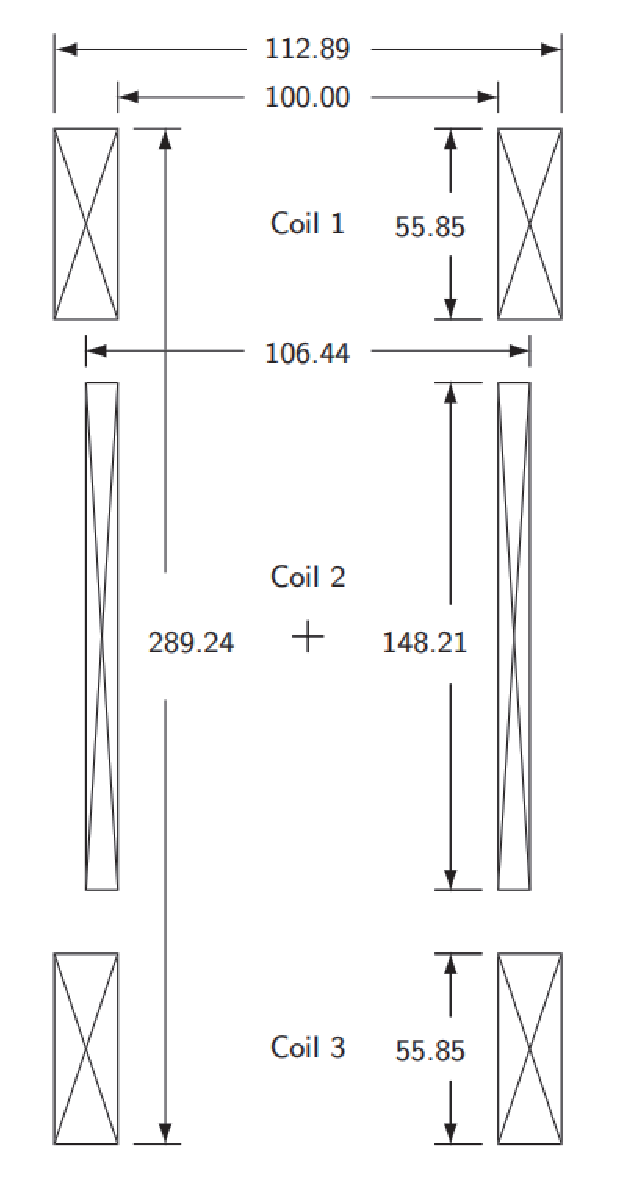
\includegraphics[scale=0.55]{chpt3/figs/fig3.25.eps}
	\caption{三个线圈组成的磁体,以mm为单位}
\end{figure}
图3.25给出了一个由三个线圈组成的空间均匀高场磁体的结构剖面。
线圈1和线圈3是完全一样的,分别位于中间线圈2的上方和下方,
用以提高中心$(0,0)$的场均匀性。
关键尺寸(mm为单位)已在图中标注。
每个线圈的$2a_1$都是$100\ \mathrm{mm}$,每个线圈的总电流密度均为
$\lambda J =2.5147×10^8\ \mathrm{A/m^2} $。
表3.4给出了使用Bobrov的程序计算得到的该磁体的场参数[3.32]。
\begin{table}[htbp]\small
\centering
\caption{场参数}
\begin{tabular}{|l|l|}
	\hline
		参数                 & 值                    \\ \hline
	中心场,$B_0$  [T] & 1.000                    \\ 
	$d^2B/dz^2\mid_0$  \qquad   [$\mathrm{T/cm^2}$]      & 0.4658$\times10^{-6} $\\ 
	$d^4B/dz^4\mid_0  $\qquad   [$\mathrm{T/cm^4}$] & 4.8450$\times10^{-5} $\\ 
	$d^6B/dz^6\mid_0 $ \qquad   [$\mathrm{T/cm^6}$]   & 1.0893$\times10^{-4} $\\
	$d^8B/dz^8\mid_0$ \qquad    [$\mathrm{T/cm^8}$]    & 1.0789$\times10^{-4}$ \\ \hline
	\end{tabular}
\end{table}

\begin{figure}[htbp]
	\centering
	\includegraphics[scale=0.6]{chpt3/figs/fig3.26.eps}
	\caption{将图3.25中的三个线圈表示为A、B、C,每个线圈的中心都位于磁体中心。线圈C的负号表示
		它的载流是与A和B反向的。尺寸以mm为单位。}
\end{figure}

图3.26给出的是用A、B和C表示的同一磁体,各线圈的中心都在$(0,0)$。
线圈A从线圈1延伸至线圈3,并包括中间的两个间隙。线圈B与线圈2一致。
因为这个新的表示法中线圈2被线圈A和线圈B表示了2次,
所以使用与线圈A和B电流相反的线圈C,以减掉1个线圈2以及那两个间隙。

a) 证明:图3.26的线圈配置和原线圈配置给出相同的中心场。线圈A、B和C的总电流密度都是$\lambda J$。
\begin{equation} %3.125
B_0 = 1.000\ \mathrm{T}=\mu_0\lambda J a_1[F_A(\alpha,\beta)+F_B(\alpha,\beta)-F_C(\alpha,\beta)]
\end{equation}

b) 应用式3.14和3.17,并用手持科学计算器计算本磁体的$d^2B/dz^2|_0$和$d^4B/dz^4|_0$。
计算值应该与表3.4使用程序计算的结果吻合。

\subsubsection{问题3.5之解}
表3.5列出了线圈A、B和C的$\alpha$和$\beta$的对应值。采用这些值,得:
%计算的F
\begin{align*}% page144
F_A(\alpha,\beta)&=0.12094421\\
F_B(\alpha,\beta)&=0.05287933\\
F_C(\alpha,\beta)&=0.11053327
\end{align*}
%表格3.5
\begin{table}[htbp]\small
\centering
\caption{场参数}
	\begin{tabular}{|c|c|c|}
		\hline
		线圈 &$ \alpha$  & $\beta $  \\ \hline
		A     & 1.12888 & 2.89244 \\ \hline
		B     & 1.06444 & 1.48212 \\ \hline
		C     & 1.12888 & 1.77548 \\ \hline
	\end{tabular}
\end{table}

a) 由式3.125,我们有:
%%
\begin{equation*}% page144
\begin{split}
B_0=&(4\pi\times 10^{-7}\ \mathrm{H/m})(2.5147\times 10^8\ \mathrm{ A/m^2})(5\times 10^{-2}\ \mathrm{m})\\
&\times(0.12094421+0.05287933-0.11053327)=1.000\ \mathrm{T}
\end{split}
\end{equation*}

b)将$\alpha$和$\beta$代入3.14a和3.14b1,我们有:
%%
 \begin{align*}% page144
F(\alpha,\beta)E_2(\alpha,\beta)_A=-0.002277367;\qquad F(\alpha,\beta)E_4(\alpha,\beta)_A=-0.000315757\\
F(\alpha,\beta)E_2(\alpha,\beta)_B=-0.007938543;\qquad F(\alpha,\beta)E_4(\alpha,\beta)_B=-0.001737981\\
F(\alpha,\beta)E_2(\alpha,\beta)_C=-0.010216278;\qquad F(\alpha,\beta)E_4(\alpha,\beta)_C=-0.002133593
\end{align*}

当所有线圈都有相同的$a_1$和$\lambda J a_1$时,3.18成为:
\begin{equation*}% S5.1
h_\zeta(\zeta)=1+\frac{\sum^{k}_{j=1}F(\alpha_j,\beta_j)E_2(\alpha_j,\beta_j)}{\sum^{k}_{j=1}F(\alpha_j,\beta_j)}\zeta^2+\cdots \tag{S5.1}
\end{equation*}

\begin{align*}
E_2(\alpha,\beta)&=\frac{F(\alpha,\beta)E_2(\alpha,\beta)_A+F(\alpha,\beta)E_2(\alpha,\beta)_B-F(\alpha,\beta)E_2(\alpha,\beta)_C}{F(\alpha,\beta)_A+F(\alpha,\beta)_B-F(\alpha,\beta)_C}\\
&=\frac{-0.002277367-0.007938543+0.010216278}{0.120924421+0.05287933-0.11053327}=0.000005822\\
E_4(\alpha,\beta)&=\frac{-0.000315757-0.001737981+0.002132363}{0.6329027}=0.001261725
\end{align*}

于是我们有:
\begin{align*}% page144
\frac{d^2B}{dz^2}\bigg|_0=2E_2\left(\frac{B_0}{a_{1}^{2}}\right)=0.4658\times 10^{-6}\ \mathrm{T/cm^2}\\
\frac{d^4B}{dz^4}\bigg|_0=24E_4\left(\frac{B_0}{a_{1}^{4}}\right)=4.8453\times 10^{-5}\ \mathrm{T/cm^4}
\end{align*}

这些数值与表3.4给出的数据完全是一致的,如果我们能勤奋的计算至第九位小数的话。

值得注意的是,在\textit{给定}磁体设计时,这里给出的分析对磁场梯度项的计算很有用,尽管乏味。
这里给出的分析形式对设计空间高均匀性磁体并不实用;
不过,它可作为开发个人设计程序的基础。

\subsection{问题3.6:直角坐标下的磁场展开}
在由图3.4定义的球坐标$(r, \theta,\phi)$下,
由嵌套线圈组成磁体产生的在无源空间的$z$向磁场$H_z$可由式3.9表示。

证明,笛卡尔坐标系下$H_z(r, \theta,\phi)$的表达式$H_z(x, y, z)$在$n=0, 1, 2$时分别为:
%%3.126
\begin{subequations}
	\begin{align}
n=0\qquad H_z(x,y,z)=&A_{0}^{0}\\
n=1\qquad H_z(x,y,z)=&A_{0}^{0}+2zA_{1}^{0}+3(A_{1}^{1}x+B_{1}^{1}y)\\
n=2\qquad H_z(x,y,z)=&A_{0}^{0}+2zA_{1}^{0}+3(A_{1}^{1}x+B_{1}^{1}y)\notag\\
&+\frac{3}{2}A_{2}^{0}(2z^2-x^2-y^2)+12z(A_{2}^{1}x+B_{2}^{1}y)\notag\\
&+15[A_{2}^{2}(x^2-y^2)+2B_{2}^{2}xy]
	\end{align}
\end{subequations}


\subsubsection{问题3.6之解}
球坐标参数$r, u = \cos\theta, s = \sin\theta, \sin\varphi,\cos\varphi$用$x,y,z$表示为:
%%S6.1
 \begin{align*}% S6.1a
&r=\sqrt{x^2+y^2+z^2}\tag{S6.1a}\\
&u=\cos\theta=\frac{z}{\sqrt{x^2+y^2+z^2}}\tag{S6.1b}\\
&s=\sin\theta=\frac{\sqrt{x^2+y^2}}{\sqrt{x^2+y^2+z^2}}\tag{S6.1c}\\
&\sin\varphi=\frac{y}{\sqrt{x^2+y^2}}\tag{S6.1d}\\
&\cos\varphi=\frac{x}{\sqrt{x^2+y^2}}\tag{S6.1e}
\end{align*}

式3.9与S6.1a-S6.1e分别对$n=0,1,2$联立,有:


$n=0$:
\begin{equation*}% S6.2a
\begin{split}
H_z(x,y,z)=&\sum^{0}_{m=0}r^0(1+0)P_{0}^{0}(u)(A_{0}^{0}\cos0 +B_{0}^{0}\sin 0)\\
=&(1)(1)(1)(A_{0}^{0})
\end{split}\tag{S6.2}
\end{equation*}

即对$n=0$,有:
 \begin{equation*}% 3.126a
H_z(x,y,z)=A_{0}^{0} \tag{3.126a}
\end{equation*}
其中,$A_0^0$表示磁体中心场$H_z(0, 0, 0)$。

$n=1$:
\begin{equation*}% s6.3a
\begin{split}
H_z(x,y,z)=&\sum^{1}_{m=0}r^1(2+m)P_{1}^{m}(A_{1}^{m}\cos m\varphi+B_{1}^{m}\sin m\varphi)\\
=&r^1(2+0)P_{1}^{0}(A_{1}^{0})+r^1(2+1)
P_{1}^{1}(A_{1}^{1}\cos\varphi+B_{1}^{1}\sin\varphi)\\
=&2ruA_{1}^{0}+3rs(A_{1}^{1}\cos\varphi+B_{1}^{1}\sin\varphi)\\
=&2\sqrt{x^2+y^2+z^2}\frac{z}{\sqrt{x^2+y^2+z^2}}A_{1}^{0}\\
&+3\sqrt{x^2+y^2+z^2}\frac{\sqrt{x^2+y^2}}{\sqrt{x^2+y^2+z^2}}\left(\frac{A_{1}^{1}x+B_{1}^{1}y}{\sqrt{x^2+y^2}}\right)\\
=&2zA_{1}^{0}+3(A_{1}^{1}x+B_{1}^{1}y)
\end{split}\tag{S6.3}
\end{equation*}

于是,在$n$不大于1时,有:
%%3.126b
\begin{equation*}% 3.126b
H_z(x,y,z)=A_{0}^{0}+2zA_{1}^{0}+3(A_{1}^{1}x+B_{1}^{1}y) \tag{3.126b}
\end{equation*}

注意,$H_z(x, y, z)$含有仅随着$z,x,y$变化的项。

$n=2$:%%S6.4
 \begin{equation*}% S6.4
 \begin{split}
H_z(x,y,z)=&\sum^{2}_{m=0}r^2(3+m)P_{2}^{m}(A_{2}^{m}\cos m\varphi+B_{2}^{m}\sin m\varphi)\\
=&r^2(3+0)P_{2}^{0}(A_{2}^{0})+r^2(3+1)P_{2}^{1}
(A_{2}^{1}\cos\varphi+B_{2}^{1}\sin\varphi)\\
&+r^2(3+2)P_{2}^{2}(A_{2}^{2}\cos 2\varphi+B_{2}^{2}\sin 2\varphi)
 \end{split} \tag{S6.4}
\end{equation*}

\begin{equation*}% S6.4b
\begin{split}
H_z(x,y,z)=&3(x^2+y^2+z^2)\frac{1}{2}\left(\frac{2z^2-x^2-y^2}{x^2+y^2+z^2}\right)A_{2}^{0}\\
&+4(x^2+y^2+z^2)\frac{3z\sqrt{x^2+y^2}}{x^2+y^2+z^2}
\left(A_{2}^{1}\frac{x}{\sqrt{x^2+y^2}}+B_{2}^{1}\frac{y}{\sqrt{x^2+y^2}}\right)\\
&+5(x^2+y^2+z^2)\frac{3(x^2+y^2)}{x^2+y^2+z^2}\left[A_{2}^{2}\left(\frac{2x^2}{x^2+y^2}-1\right)+B_{2}^{2}\frac{2xy}{x^2+y^2}\right]\\
=&\frac{3}{2}A_{2}^{0}(2z^2-x^2-y^2)+12z(A_{2}^{1}x+B_{2}^{1}y)+15[A_{2}^{2}(x^2-y^2)+2B_{2}^{2}xy]
\end{split}\tag{S6.4b}
\end{equation*}

累加S6.2b, S6.3b和S6.4b,我们得到$n$值不大于2的情况:
\begin{equation*}% 3.126c
\begin{split}
H_z(x,y,z)=&A_{0}^{0}+2zA_{1}^{0}+3(A_{1}^{1}x+B_{1}^{1}y)\\
&+\frac{3}{2}A_{2}^{0}(2z^2-x^2-y^2)+12z(A_{2}^{1}x+B_{2}^{1}y)\\
&+15[A_{2}^{2}(x^2-y^2)+2B_{2}^{2}xy]
\end{split}\tag{3.126c}
\end{equation*}

注意到,当在$n=0,1$和$2$下计算$H_z(x, y, z)$时,它包含随$x, y, z, z^2, x^2, y^2, zx, zy$和$xy$变化的项。


\subsection{问题3.7:Notched螺管}
Helmholtz线圈的准则---在关于螺管中心对称的位置放置载流元以在中心区域产生空间均匀场
---是notched螺管线圈设计的基础。
很多MRI和NMR磁体都是notched螺管设计的变种。

对一个绕组内半径$a_1$,外半径$a_2$,总长度$2b$,总电流密度$\lambda J$的简单螺管,
回想到前面3.13a和3.13b给出的中心轴向场$H_0\equiv H_z(0, 0)$:
%%3.13a/b
 \begin{equation*}% 3.13a
H_0=\lambda Ja_1F(\alpha,\beta) \tag{3.13a}
\end{equation*}
\begin{equation*}% 3.13b
F(\alpha,\beta)=\beta\ln\left(\frac{\alpha+\sqrt{\alpha^2+\beta^2}}{1+\sqrt{1+\beta^2}}\right)\tag{3.13b}
\end{equation*}

考虑到对称性以及前面讨论3.4给出的叠加技术,证明
如图3.27所示的具有均匀电流密度$\lambda J$的notched螺管的$H_z(0, z_1)$的表达式为:
%%3.127
\begin{equation}% 3.127
\begin{split}
H_z(0,z_1)=&\frac{1}{2}\lambda J a_1\left[F(\alpha_1,\beta_1+\gamma_1)+F(\alpha_1,\beta_1-\gamma_1)\right]\\
&-\frac{1}{2}\lambda Ja_3
\left[F(\alpha_2,\beta_2+\gamma_2)+F(\alpha_2,\beta_2-\gamma_2)\right]
\end{split}
\end{equation}
式中,$\alpha_1=a_2/a_1,\beta_1=b_1/a_1,\gamma_1=z_1/a_1,\alpha_2=a_2/a_3,\beta_2=b_2/a_3,\gamma_2=z_1/a_3$。螺管参数$a_1, a_2, a_3, b_1, b_2$如图3.27的定义。

一个简单的notched线圈除了几个空间均匀度系数,仅有少数几个自由度可迫零,但那些2阶和4阶量可以很好的破零。

\begin{figure}[htbp]
	\centering
	\includegraphics[scale=0.4]{chpt3/figs/fig3.27.eps}
	\caption{一个notched螺管的几何形状。}
\end{figure}


\subsubsection{问题3.7之解}
为了解出$H_z(0,z_1)$,我们可以把螺管分成四个单螺管,其截面参数按角点设计如下:

\textbf{螺管1}:ABDC,有$\alpha_1=a_2/a_1=\alpha,\beta_1=(b_1+z_1)/a_1=\beta+\gamma$,其中
$\beta=b_1/a_1,\gamma=z_1/a_1$;

\textbf{螺管2}:BEFD,有$\alpha_2=a_2/a_1=\alpha,\beta_2=(b_1-z_1)/a_1=\beta-\gamma$;

\textbf{螺管3}:IGDL,有$\alpha_3=a_2/a_3=\alpha^\prime,\beta_3=(b_2+z_1)/a_3=\beta^\prime+\gamma^\prime$,其中$\beta^\prime=b_2/a_3,\gamma^\prime=z_1/a_3$;

\textbf{螺管4}:GKHD,有$\alpha_4=a_2/a_3=\alpha^\prime,\beta_4=(b_2-z_1)/a_3=\beta^\prime-\gamma^\prime$.

我们注意到,所有螺管中$J$都有相同的幅值,但螺管3和4与螺管1和2有相反的符号。
同时,所有的螺管都不再有凹槽。

\textbf{螺管1的磁场}:长$2b=b_1+z_1$的螺管1产生的$H_z(0, z_1)$是具有相同参数$a_1, a_2,\lambda J$而长度
为$2b = 2(b_1+z_1)$的螺管产生的中心场的一半。
这从一个长为$2b$的非notched螺管的中心场$H_z(0, 0)$是两部分螺管产生的场(一部分来自$z=−b$到$0$,另一部分
来自$0$到$z=b$)之和这一点看的更清楚。
也即,螺管的每一半各贡献总场$H_z(0, 0)$的50\%。 于是:
\begin{equation*}
H_{z}(0,z_{1})|_{1}=\frac{1}{2}\lambda Ja_{1}F(\alpha,\beta+\gamma)\tag{S7.1}
\end{equation*}

\textbf{螺管2的磁场}:在$(0, z_1)$,$H_z$中来自长度$2b = b_1−z_1$的螺管2的部分是具有相同$a_1, a_2,\lambda J$而长度为
$2b = 2(b_1−z_1)$的螺管的中心场的一半。
\begin{equation}
H_{z}(0,z_{1})|_{2}=\frac{1}{2}\lambda Ja_{1}F(\alpha,\beta-\gamma)\tag{S7.2}
\end{equation}

\textbf{螺管3的磁场}:在$(0, z_1)$,$H_z$中来自长$2b=b_2+z_1$的螺管3的部分是
具有相同$a_3, a_2,\lambda J$而长度为$2b=2(b_2+z_1)$的螺管的中心场的一半。
因为$J$是反向的,我们有:
\begin{equation}
H_{Z}(0,z_{1})|_{3}=-\frac{1}{2}\lambda Ja_{3}F(\alpha',\beta'+\gamma')\tag{S7.3}
\end{equation}

\textbf{螺管4的磁场}:在$(0, z_1)$,$H_z$来自长$2b = b_2−z_1$的螺管4的部分是
其他参数相同而长为$2b = 2(b_2−z_1)$的螺管的中心场的一半。
\begin{equation}
H_{z}(0,z_{1})|_{4}=-\frac{1}{2}\lambda Ja_{3}F(\alpha',\beta'-\gamma')\tag{S7.4}
\end{equation}

\textbf{Notched螺管的磁场}

原notched螺管产生的$H_z(0,z_1)$于是可以由上四式S7.1-S7.4之和给出:
\begin{equation*}%3.127
\begin{split}
 H_{z}(0,z_{1}) =&H_{z}(0,z_{1})|_{1}+H_{z}(0,z_{1})|_{2}+H_{z}(0,z_{1})|_{3}+H_{z}(0,z_{1})|_{4} \\
=&\frac{1}{2}\lambda J a_{1}[F(\alpha,\beta+\gamma)+F(\alpha,\beta-\gamma)] \\%page115
&-\frac{1}{2}\lambda J a_{3}[F(\lambda',\beta'+\gamma')+F(\alpha',\beta'-\gamma')]
\end{split} \tag{3.127}
\end{equation*}



\subsection{讨论3.7:饼式线圈磁体的磁场分析}
本节应用讨论3.4中的叠加技术,推导可用于计算一个由$2N$个饼式线圈($N$个双饼)组成的螺管磁体
的磁场误差系数的轴向场表达式。
由于Bi2223和YBCO高温超导带都是带状的,
由之绕制饼式线圈组成磁体是实现空间高均匀度磁体(例如NMR和MRI磁体)的一个可行途径[3.33, 3.34]。
饼式线圈是``薄''的长方形截面导体的理想形式。

在这个分析中,各饼尺度一致---$2a_1;2a_2;2b=w$(带材宽度),饼线圈绕组中的$\lambda J$也相同。
相邻线圈间距为$\delta$。图3.28给出了一个由$2N$个单饼组成的磁体的剖面示意图。

在推导磁场方程时认为所有的饼都对磁体原点居中。我们采用下面的简化记法,将$F(\alpha,\beta)/{\beta}$简记为:
\begin{equation}
\frac{F(\alpha,\beta)}{\beta}\equiv \ln(\alpha,\beta)=\ln\left[\frac{\alpha+\sqrt{\alpha^2+\beta^2}}{1+\sqrt{1+\beta^2}}\right]\\%(3.128)
\end{equation}

我们定义一个无量纲轴向磁场参数$\eta(\zeta)\equiv H(z)/(\lambda J a_1)$,其中$\zeta\equiv z/a_1$:
\begin{equation*}
\eta(\xi)\equiv \frac{H(Z)}{\lambda Ja_{1}}=\beta \ln(\alpha,\beta)\left[1+\sum_{j=1}^{n} E_{2j}(\alpha,\beta)\xi^{2j}\right]\tag{3.128b}
\end{equation*}

因为使用了$\ln(\alpha,\beta)$,式3.128b是一个与3.13a形式略有不同的无量纲场表达式。
\begin{figure}[htbp]
	\centering
	\includegraphics[scale=0.4]{chpt3/figs/fig3.28.eps}
	\caption{由$2N$个单饼(或$N$个双饼)组成的磁体,各饼尺寸一致---$2a_1;2a_2;2b=w$(带材宽度),且有相同的$\lambda J$。}
\end{figure}

\begin{figure}[htbp]
	\centering
	\includegraphics[scale=0.5]{chpt3/figs/fig3.29.eps}
	\caption{将双饼磁体视为$2b=2w+\delta$的线圈2减去$2b^\prime=\delta$的线圈$2^\prime$。}
\end{figure}

\textbf{第一步:二饼磁体---饼1和饼2}

首先考虑最简单的情况:一个由两个饼$P1$和$P2$组成的磁体。
采用讨论3.4中的叠加技术,具有间隙$\delta$(图3.29最左侧)的原始磁体与两个无间隙螺管等价:
高为$2b_2 = w +\delta$的线圈2(中部)减去高为$2b_2^\prime = \delta^\prime$的线圈$2^\prime$。
下标2为了标明考虑的磁体包括两个饼式线圈。
图3.29中的每个线圈仅给出了高度($2b$)是因为高度是唯一的有关参数:
即对线圈2,有$\beta_2=(2w+\delta)/2a_1$;对线圈$2^\prime$,有$\beta_2=\delta/2a_1$。

与两个线圈有关的无量纲轴向场$\eta_2(\zeta)$为:
\begin{equation}
\eta_{2}(\zeta)=[\eta(\zeta)]_{2}-[\eta'(\zeta)]_{2}\\%(3.129)
\end{equation}

根据3.128b式,我们有:
\begin{subequations}
	\begin{align}
{[\eta(\zeta)_{2}]}&=\beta_{2}\ln(\alpha,\beta_{2})\left[1+\sum_{j=1}^{n}E_{2j}(\alpha,\beta_{2})\zeta_{2j}\right]\\
{[\eta'(\zeta)]}_{2}&=\beta'_{2}\ln(\alpha,\beta'_{2})\left[1+\sum_{j=1}^{n}E_{2j}(\alpha,\beta'_{2})\zeta^{2j}\right]%3.130b
	\end{align}
\end{subequations}

联立3.129和3.130,有:
\begin{equation}
\begin{split}
\eta_{2}(\zeta)=&[\beta_{2}\ln(\alpha,\beta_{2})-\beta'_{2}\ln(\alpha,\beta'_{2})]\\
&+\sum_{j=1}^{n}[\beta_{2}\ln(\alpha,\beta_{2})E_{2j}(\alpha,\beta_{2})-\beta'_{2}\ln(\alpha,\beta'_{2})]E_{2j}(\alpha,\beta^\prime_{2})\zeta^{2j}%(3.131)
\end{split}
\end{equation}

\textbf{第二步:四饼磁体---再加上饼3和饼4}

接下来,我们考虑一个由四个饼组成的磁体。
如图3.30所示,新磁体是第一步中的二饼磁体上下各加一个饼组成的。
如图3.30所给出的,这两个新的饼可以建模为$2b=4w+3\delta$的线圈4减去
$2b=2w+3\delta$的线圈$4^\prime$。于是,对线圈4,有$\beta_4=(4w+3\delta)/2a_1$;
对线圈$4^\prime$,有$\beta_4^\prime=(2w+3\delta)/2a_1$。
\begin{figure}[htbp]
	\centering
	\includegraphics[scale=0.5]{chpt3/figs/fig3.30.eps}
	\caption{将四饼磁体视为如图3.29所示的二饼磁体加上$2b=4w+3\delta$的线圈4减去
$2b=2w+3\delta$的线圈$4^\prime$得到的磁体。}
\end{figure}

来自所有四个线圈的总的无量纲轴向磁场$\eta_4(z)$为:
\begin{equation}
\eta_{4}(z)=[\eta(\zeta)]_{2}-[\eta'(\zeta)]_{2}+[\eta(\zeta)]_{4}-[\eta'(z)]_{4}\\%(3.132)
\end{equation}
其中,
\begin{subequations}
	\begin{align}
{[\eta(\zeta)]}_{4}=&\beta_{4}\ln(\alpha,\beta_{4})\left[1+\sum_{j=1}^{n}E_{2j}(\alpha,\beta_{4})\zeta^{2j}\right]\\
{[\eta'(\zeta)]}_{4}=&\beta'_{4}\ln(\alpha,\beta'_{4})\left[1+\sum_{j=1}^{n}E_{2j}(\alpha,\beta'_{4})\zeta^{2j}\right]
	\end{align}
\end{subequations}

联立3.130和3.133,我们得到:
\begin{equation}
\begin{split}
\eta_{4}(\zeta)=&[\beta_{2}\ln(\alpha,\beta_{2})+\beta_{4}\ln(\alpha,\beta_{4})]-[\beta'_{2}\ln(\alpha,\beta'_{2})+\beta'_{4}\ln(\alpha,\beta'_{4})]\\
&+\sum_{j=1}^{n}\bigg\{[\beta_{2}\ln(\alpha,\beta_{2})E_{2j}(\alpha,\beta_{2})+\beta_{4}\ln(\alpha,\beta_{4})E_{2j}(\alpha,\beta_{4})]\\
&-[\beta'_{2}\ln(\alpha,\beta'_{2})E_{2j}(\alpha,\beta'_{2})+\beta'_{4}\ln(\alpha,\beta'_{4})E_{2j}(\alpha,\beta'_{4})]\bigg\}\zeta^{2j}%(3.134)
\end{split}
\end{equation}

\textbf{第三步:$2N$饼磁体---加上最后两个饼}

图3.31给出了$2N$饼磁体加入最后两个饼$(2N−1)$和$2N$的模型。
线圈$2N$有$2b_N =2Nw+(2N−1)\delta$,由此$\beta_{2N}=[2Nw+(2N−1)\delta]/2a_1$;
线圈$2N^\prime$有$2b_N^\prime=2(N-1)w+(2N−1)\delta$,由此$\beta_{2N}^\prime=[2(N-1)w+(2N−1)\delta]/2a_1$。

由$N$个双饼组成的$2N$饼磁体的轴向磁场表达式:
\begin{equation}
\eta_{2N}(\zeta)=\sum_{k=1}^{N}\{[\eta(\zeta)]_{2k}-[\eta'(\zeta)]_{2k}\}\\%(3.135)
\end{equation}

本分析中,我们假设双饼的两个饼间距离和相邻双饼之间的距离是相等的。
\begin{figure}[htbp]
	\centering
	\includegraphics[scale=0.4]{chpt3/figs/fig3.31.eps}
	\caption{将$2N$饼磁体视为$2(N-1)$饼磁体加上线圈$2N$再减去线圈$2N^\prime$所得的磁体。}
\end{figure}

我们可以类似3.134的形式表示3.135:
\begin{equation}
\begin{split}
\eta_{2N}(\zeta)=&\sum_{k=1}^{N}\bigg\{\left[\beta_{2k}\ln(\alpha,\beta_{2k})-\beta'_{2k}\ln(\alpha,\beta'_{2k})\right]\\
&+\sum_{j=1}^{n}[\beta_{2k}\ln(\alpha,\beta_{2k})E_{2j}(\alpha,\beta_{2k})-\beta'_{2k}\ln(\alpha,\beta'_{2k})E_{2j}(\alpha,\beta'_{2k})]\bigg\}\zeta^{2j}%(3.136)
\end{split}
\end{equation}
式中,
\begin{equation*}
\beta_{2k}=\frac{2kw+(sk-1)\delta}{2a_1};\qquad \beta'_{2k}=\frac{2(k-1)w+(2k-1)\delta}{2a_{1}}
\end{equation*}

式3.136也可以写作:
\begin{equation}
\frac{\eta_{2N}(\zeta)}{\eta_{2N}(0)}=\{1+[E_{2}]_{2N}\zeta^2+\cdots+[E_{2n}]_{2N}\zeta^{2n}\}\\%(3.137)
\end{equation}
式中,$\eta_{2N}(0)$是无量纲中心场。$[E_{2n}]_{2N}$是第$n$阶总体误差系数。
$\eta_{2N}(\zeta=0)$和$[E_{2n}]_{2N}$为:
\begin{subequations}
	\begin{align}
\eta_{2N}(0)&=\sum_{k=1}^{N}[\beta_{2k}\ln(\alpha,\beta_{2k})-\beta'_{2k}\ln(\alpha,\beta'_{2k})]\\%3.138a)
{[E_{2n}]}_{2N}&=\frac{\sum_{k=1}^{N}[\beta_{2k}\ln(\alpha,\beta_{2k})E_{2n}(\alpha,\beta_{2k})-\beta'_{2k}\ln(\alpha,\beta'{2k})E_{2n}(\alpha,\beta'_{2k})]}{\sum_{k=1}^{N}[\beta_{2k}\ln(\alpha,\beta_{2k})-\beta'_{2k}\ln(\alpha,\beta'_{2k})]}%(3.138b)
	\end{align}
\end{subequations}

于是,3.138b给出了一个计算由$2N$个一致饼式线圈(各饼有相同的$2a_1,2b=w,\alpha,\beta$,相邻间距$\delta$)组成的磁体的第$n$阶误差系数的表达式。


\subsection{问题3.8:理想二极磁体}
本问题研究理想二极磁体。此磁体无限长(从而无边缘效应)、绕组厚度为零、磁场由纵向表面电流产生、
磁场方向与二极磁体的轴垂直。
实际二极磁体的磁场和力的计算远比理想二极磁体复杂;
不过,除了在端部的复杂情况,理想二极磁体给出了二极磁体的多数关键特征。
二极磁体用于需要与磁体轴向垂直方向均匀磁场的系统,例如高能粒子加速器[3.35–3.40]和发电机[3.41–3.43]。

一个半径为$R$、``零''绕组厚度的长(二维)二极磁体由二极壳($r=R$)上的$z$向表面电流励磁。
室温孔内($r<R$)的磁场$\vec{H}_{d1}$以及壳外的磁场$\vec{H}_{d2}$为:
\begin{subequations}
	\begin{align}
\vec{H}_{d1}&=H_{0}(\sin\theta\vec{\imath}_{r}+\cos\theta\vec{\imath}_{\theta})\\%3.139a)
\vec{H}_{d2}&=H_{0}\left(\frac{R}{r}\right)^2(\sin\theta\vec{\imath}_{r}-\cos\theta\vec{\imath}_{\theta})%(3.139b)
	\end{align}
\end{subequations}

二维坐标的定义如图3.32。$+z$方向指向纸面外。在解答下面的问题时,忽略边缘效应。

a) 画出二极磁体在$r<R$和$r>R$两个区域的场线。

b) 证明$r=R$处的表面电流的表达式为:
\begin{equation}
\vec{K}_{f}=-2H_{0}\cos\theta\vec{\imath}_{z}\\%(3.140)
\end{equation}

标出电流方向,$\vec{K}_f$如果是$+z$方向,画圈(o);反之,画叉(×)。

c) 证明作用在壳载流单元上的单位长度的Lorentz力密度$\vec{f}_L$[$\mathrm{N/m^2}$]为:
\begin{equation}
\vec{f}_{L}=-\mu_{0}H_{0}^{2}\sin 2\theta\vec{\imath}_{\theta}\\%(3.141)
\end{equation}

\begin{figure}[htbp]
	\centering
	\includegraphics[scale=0.5]{chpt3/figs/fig3.32.eps}
	\caption{圆柱坐标系;$+z$朝向纸面外。}
\end{figure}

d) 证明施于右半部分($−90^\circ<\theta<90^\circ$)的$x$向单位二极长度净
Lorentz力$\vec{F}_{Lx}[\mathrm{N/m}]$为:
\begin{equation}
F_{Lx}=\frac{4R\mu_{0}H_{0}^{2}}{3}%(3.142)
\end{equation}

e) 证明单位二极长度储存的总磁能表达式$E_m[\mathrm{J/m}]$为:
\begin{equation}
E_{m}=\frac{\pi R^{2}B_{0}^{2}}{\mu_{0}}\\%(3.143)
\end{equation}

在$B_0=5\ \mathrm{T},R=20\ \mathrm{mm}$时计算$E_m$。
同时,由$E_m$计算一个长为$10\ \mathrm{m}$、载流$I_{op}=5000\ \mathrm{A}$的二极磁体的电感$L$。

为了减少二极磁体外部的磁场,在极外安装一个厚为$d$的铁扼($\mu=\infty$),如图3.33所示。

f) 证明,新条件下在二极内部产生\textit{同样}的磁场$\vec{H}$,需要的$\vec{K}_{f1}$恰为3.140的一半。
解释为什么电流减小了。

g) 实际中,铁扼不可能在无限的$H_0$下保持高$\mu$值。证明,为了铁扼不饱和,
最小的$d_m$为:
\begin{equation}
d_{m}=R\left(\frac{H_{0}}{M_{sa}}\right)%(3.144)
\end{equation}
式中,$M_{sa}$是铁扼材料的饱和磁化强度。在以下条件下计算$d_m$:$\mu_0 H_0=5\ \mathrm{T};\mu_0 M_{sa}=1.2\ \mathrm{T}; R=20\ \mathrm{mm}$。
\begin{figure}[htbp]
	\centering
	\includegraphics[scale=0.5]{chpt3/figs/fig3.33.eps}
	\caption{理想二极磁体外安装厚度为$d$的铁扼。}
\end{figure}

\subsubsection{问题3.8之解}
a) 场线如图3.34a示意。磁场的法向($r$向)分量在边界处($r=R$)处是连续的。

b) 磁场的切向方向($\theta$向)在$r=R$处不连续,差值为该处的表面电流密度$\vec{K}_f$,
根据2.6,有:
\begin{equation*}
\vec{K}_{f}=\vec{\imath}_{r}\times(\vec{H}_{d2}-\vec{H}_{d1})=\vec{\imath}_{r}\times-2H_{0}\cos\theta\vec{\imath}_{\theta}\\
=-2H_{0}\cos\theta\vec{\imath}_{z}\tag{3.140}
\end{equation*}

如图3.34b,$\vec{K}_f$在$-90^\circ<\theta<90^\circ$部分指向$-z$向,在
$90^\circ<\theta<270^\circ$部分指向$+z$向。
\begin{figure}[htbp]
	\centering
	\includegraphics[scale=0.6]{chpt3/figs/fig3.34.eps}
	\caption{理想二极磁体。a) 内外场;b)表面电流密度矢量;c)力矢量。}
\end{figure}

c) $\vec{f}_L$由$\vec{K}_f\times\mu_0 \vec{H}_d$给出,其中$\mu_0 \vec{H}_d=\mu_0(\vec{H}_{d1}+\vec{H}_{d2})/2$:
\begin{align*}
\vec{f}_{L}=&\vec{K}_{f}\times\mu_{0}H_{0}\sin\theta\vec{\imath}_{r}\tag{S8.1}\\
=&-2\mu_{0}H_{0}^{2}\cos\theta \sin\theta\vec{\imath}_{\theta}\\
=&-\mu_{0}H_{0}^{2}\sin 2\theta\vec{\imath}_{\theta}\tag{3.141}
\end{align*}

可见,$\vec{f_L}$无$r$分量,仅有$\theta$分量(图3.34c)。
同时,力密度在$\theta=\pi/4+n\pi/2$处最大,而在$\theta=0+n\pi/2$时为零,式中$n=0, 1, 2, 3$。
合力$\propto\int f_L(\theta)d\theta$,在$\theta=0$和$180^\circ$时取最大值。

d) 从图3.34c明显可见,施于右半部分的单位长度Lorentz力是$+x$方向的:
\begin{align*}
F_{Ldx}&=\int\vec{f}_{L}\cdot\vec{\imath}_{x}dx=-R\int_{\frac{-\pi}{2}}^{\frac{\pi}{2}}f_{L\theta}\sin\theta d\theta\tag{S8.2a}\\
&=-2R\int_{0}^{\frac{\pi}{2}}f_{L\theta}\sin\theta d\theta=4R\mu_{0}H_{0}^{2}\int_{0}^{\frac{\pi}{2}}\cos\theta \sin^{2}\theta d\theta\tag{S8.2b}
\end{align*}

由S8.2b,我们得:
\begin{equation*}
F_{Lx}=\frac{4R\mu_{0}H_{0}^{2}}{3}\tag{3.142}
\end{equation*}

施于左半部分的净Lorentz力和施于右半部分的Lorentz力的幅值相同但指向$-x$向。
也就是说,存在一个很大的力试图将双极磁体的两部分拉开。
实际上,用于承受这个力的支撑结构的设计是双极磁体设计的关键点之一。

e) $E_m [\ \mathrm{J/m}]$可以通过对磁能密度$\mu_0|H(r,\theta)|^2/2$在垂直于二极轴的整个表面
(从$r=0$到$r=\infty$;从$\theta=0$到$\theta=2\pi$)积分获得。
\begin{align*}
E_{m}=&\frac{\mu_{0}}{2}\int_{0}^{R}|H_{d1}|^{2}2\pi rdr+\frac{\mu_{0}}{2}\int_{R}^{\infty}|H_{d2}|^{2}2\pi rdr\tag{S8.3a}\\%(S8.3a)
=&\frac{\mu_{0}}{2}H_{0}^{2}\pi R^{2}+\frac{\mu_{0}}{2}H_{0}^{2}\pi R^{2}\tag{S8.3b}\\%(S8.3b)
=&\mu_{0}\pi R^{2}H_{0}^{2}=\frac{\pi R^{2}B_{0}^{2}}{\mu_{0}}\tag{3.143}%(3.143)
\end{align*}

从S8.3b可知,存储的总磁能可以均分为二极壳内外两部分。
我们可以想象,二极内流动电流的一半用来产生$H_{d1}$而另一半用来产生$H_{d2}$。
代入$\mu_0 H_0=B_0=5\ \mathrm{T},R=20\ \mathrm{mm}$,有:
\begin{equation*}
E_{m}=\frac{\pi(2\times 10^{-2}\ \mathrm{m})^{2}(5\ \mathrm{T})^{2}}{4\pi\times10^{-7}\ \mathrm{H/m}}=25\ \mathrm{kJ/m}
\end{equation*}

对于一个5 T二极磁体,如果长10 m,则总存储磁能变为250 kJ。总磁能即二极磁体的总电感储能。
\begin{equation*}
\frac{1}{2}LI_{op}^{2}=250\ \mathrm{kJ}\tag{S8.4}%(S8.4)
\end{equation*}

代入$I_{op}=5000\ \mathrm{A}$解出$L$,有:
\begin{equation*}
L=\frac{2(250\times10^{3}\ \mathrm{J})}{(5000\ \mathrm{A})^{2}}=20\ \mathrm{mH}
\end{equation*}

在3.7.3节已给出理想二极磁体单位长度的自感: 
\begin{equation*}
L_{\ell}=\frac{1}{8}\mu_{0}\pi N^{2}\tag{3.87}%(3.87)
\end{equation*}

代入$L_{\ell}(=2\ \mathrm{mH/m})$以及$20\ \mathrm{mH}$,解出$N$,
我们得到在$I_{op} = 5000\ \mathrm{A}$时$N\simeq 64$。
如果二极磁体的运行电流是$1000$ A,那么磁体的电感必须是$0.5$ H;
它的绕组匝数将是$20\ \mathrm{mH}$二极磁体匝数的5倍:$N\simeq 318$。

f) 因为$\mu=\infty$,以及在$R< r< R+d$时$\vec{H}_{d2}=0$,如果屏蔽足够厚而不会饱和,
那么对$r>R+d$也有$\vec{H}_{d2}=0$。$\vec{H}_{d1}$仍为前面的形式。明显:
\begin{equation*}
\vec{K}_{f1}=-H_{0}\cos\theta\vec{\imath}_{\theta}\tag{S8.5}%(S8.5)
\end{equation*}
这恰好是3.140中给出$\vec{K}_f$的一半。
考虑两种情况下要求的表面电流,我们可以作如下解释:全部用于产生室温孔场$-2H_0\cos\theta$的
表面电流中,有一半来自铁芯磁化的``表面电流"、

g) 进入径向厚度为$d$的铁扼位于$0$至$\theta=90^\circ$部分的全部单位长度磁通$[\ \mathrm{Wb/m}]$
须不大于$\mu_0 M_{sa}d$,即:
\begin{equation*}
R\mu_{0}H_{0}\int_{0}^{\frac{\pi}{2}}\sin\theta d\theta=R\mu_{0}H_{0}\leq\mu_{0}M_{sa}d\tag{S8.6}%(S8.6)
\end{equation*}

于是,铁扼的最小厚度为:
\begin{equation*}
d_{m}=R\left(\frac{H_{0}}{M_{sa}}\right)\tag{3.144}%(3.144)
\end{equation*}

代入$R=20\ \mathrm{mm}, \mu_0 H_0=5\ \mathrm{T}, \mu_0 M_{sa}=1.2\ \mathrm{T}$,我们有:
\begin{equation*}
d_{m}=83\ \mathrm{mm} 
\end{equation*}

从表2.5可知,在$\mu_0 M=1.25\ \mathrm{T}$时,as-cast钢的磁导率为$180\mu_0$。尽管不是无限大,
但对于满足我们的$\mu=\infty$假设是足够用了。

\subsection{问题3.9:理想四极磁体}
本问题研究一个理想四极磁体,该磁体无限长(无边缘效应)、零绕组厚度、纵向表面电流产生的磁场垂直于磁场轴线。
类似于二极磁体,四极磁体主要用于粒子加速器[3.35, 3.39, 3.44–3.46]。
如下文f)所论及的,四极磁体用于聚焦带电粒子束。

一个半径为$R$、零绕组厚度的``长"四极磁体由四极磁体壳体上($r=R$)沿$z$向流动的表面电流励磁。
室温孔内($r<R$)的磁场$\vec{H}_{q1}$和壳外($r>R$)的磁场$\vec{H}_{q2}$分别为:
\begin{subequations}
	\begin{align}
\vec{H}_{q1}&=H_{0}\left(\frac{r}{R}\right)(\sin 2\theta\vec{\imath}+\cos 2\theta\vec{\imath}_{\theta})\\%(3.145a)
\vec{H}_{q2}&=H_{0}\left(\frac{R}{r}\right)^{3}(\sin 2\theta\vec{\imath}_{r}-\cos 2\theta\vec{\imath}_{\theta})%(3.145b)
	\end{align}
\end{subequations}

在解答下列问题时,忽略边缘效应。

a) 大致画出四极磁体内外区域的场线。 

b) 证明$r=R$处的表面电流$\vec{K}_f$为:
\begin{equation}
\vec{K}_{f}=-2H_{0}\cos 2\theta\vec{\imath}_{z}%(3.146)
\end{equation}

大致画出电流的方向,在$\vec{K}_f$是$+z$向(指向纸面外)时画圈(o);反之,画叉(×)。

c) 证明施加于壳体载流元上的单位长度Lorentz力密度的表达式为:
\begin{equation}
\vec{f}_{L}=-\mu_{0}H_{0}^{2}\sin 4\theta\vec{\imath}_{\theta}%(3.147)
\end{equation}

d) 证明质子沿磁体中心以近乎光速$c$在$+z$向运动时,$x$向``磁弹簧系数"$k_{Lx}$的表达式为:
\begin{equation}
k_{Lx}\simeq\frac{qc\mu_{0}H_{0}}{R}%(3.148)
\end{equation}

e) 类似的,证明质子沿磁体中心以近乎光速$c$在$+z$向运动时,$y$向``磁弹簧系数"$k_{Ly}$的表达式为:
\begin{equation}
k_{Ly}\simeq-\frac{qc\mu_{0}H_{0}}{R}%(3.149)\\
\end{equation}

f) 通过阐明$k_{Lx}$和$k_{Ly}$是不稳定还是可恢复的,描述四极磁体在带电粒子加速器中的作用。

\subsubsection{问题3.9之解}
a)场线如图3.35a所示。对于理想情况,$r$分量在$r=R$处室连续的。

b)磁场的$\theta$分量在边界上的不连续等价于$r=R$处的表面电流密度,即:
\begin{equation*}
\begin{split}
\vec{K}_{f}&=\vec{\imath}_{r}\times(\vec{H}_{q2}-\vec{H}_{q1})=\vec{\imath}_{r}\times-2H_{0}\cos 2\theta\vec{\imath}_{\theta}\\
&=-2H_{0}\cos 2\theta\vec{\imath}_{z}%(3.146)
\end{split} \tag{3.146}
\end{equation*}

$\vec{K}_f$矢量在磁壳体上改变四次方向(图3.35b)。
\begin{figure}[htbp]
	\centering
	\includegraphics[scale=0.7]{chpt3/figs/fig3.35.eps}
	\caption{a) 四极磁体的内外磁场; b)磁体内的表面电流密度矢量; c) 磁体中力的方向。}
\end{figure}

c) $\vec{f}_L$由$r=R$处$\vec{K}_f$与$\mu_0 \vec{H}$的叉积给出。
在$r=R$处,平均场$(\vec{H}_{q1}+\vec{H}_{q2})/2$就是$\vec{H}=H_0 \sin 2\theta\vec{\imath}_r$,因为
$\vec{H}_{q1}$与$\vec{H}_{q2}$的$r$分量相抵消。注意到$\vec{K}_f=-2H_0 \cos 2\theta\vec{\imath}_z$,我们有:
\begin{equation*}
\vec{f}_{L}=-2\mu_{0}H_{0}^{2}\sin 2\theta \cos 2\theta\vec{\imath}_{\theta}
=-\mu_{0}H_{0}^{2}\sin 4\theta\vec{\imath}_{\theta}\tag{3.147}%(3.147)
\end{equation*}

$\vec{f}_L$的分布情况见图3.35c。

d)我们可以将$x$方向的磁弹簧系数定义为: 
\begin{equation*}
k_{Lx}=-\frac{\partial F_{Lx}}{\partial x}\tag{S9.1}%(S9.1)
\end{equation*}

电荷为$q$的质子以近乎光速$c$在$z$向运动时,受到的$x$向Lorentz力密度$F_{Lx}$为:
\begin{equation}
F_{Lx}\simeq[q(c\vec{\imath}_{z})\times\mu_{0}H_{q1}\vec{\imath}_{\theta}]_{\theta=0}
\simeq-qc\mu_{0}H_{0}\left(\frac{r}{R}\right)\vec{\imath}_{x}\tag{S9.2}%(S9.2)
\end{equation}

于是$k_{Lx}$为:
\begin{equation}
k_{Lx}=-\frac{\partial F_{Lx}}{\partial x}=-\frac{\partial F_{Lx}}{\partial r}
\simeq \frac{qc\mu_{0}H_{0}}{R}\tag{3.148}%(3.148)
\end{equation}

e) 在$y$向($r$向在$\theta=90^\circ$时),$F_{Ly}$为:
\begin{equation}
F_{Ly}\simeq[q(c\vec{\imath}_{z})\times\mu_{0}H_{q1}\vec{\imath}_{\theta}]_{\theta=\frac{\pi}{2}}
\simeq qc\mu_{0}H_{0}\left(\frac{r}{R}\right)\vec{\imath}_{y}\tag{S9.3}%(S9.3)
\end{equation}

于是$k_{Ly}$为:
\begin{equation}
k_{Ly}=-\frac{\partial F_{Ly}}{\partial y}=-\frac{\partial F_{Ly}}{\partial r}
\simeq-\frac{qc \mu_{0}H_{0}}{R}\tag{3.149}%(3.149)
\end{equation}

f) $F_{Lx}$是恢复性的;但$F_{Ly}$是不稳定的,会令粒子束在$y$向发散。
在因此加速环中四极磁体成对使用,一个用于在$x$向聚焦,紧跟另一个在$y$向聚焦,净效果是在两个方向都聚焦了。




\subsection{讨论3.8:双跑道线圈磁体}
这里我们讨论一个由在磁体轴向正交平面方向相距$2c$的平行的两个长\textit{理想}``跑道"线圈组成的磁体。
``跑道线圈''得名自导体末端绕过$180^\circ$回到起点,就像跑道一样。
和二极磁体不同,它的绕组位于同一平面,即``平"的。
平的绕组让它相比于二极磁体更容易绕制,故而更适合用于发电机和电动机[3.47–3.50]。
跑道线圈同样也适用于磁悬浮[3.51–3.53]。

图3.36给出了由两个理想跑道线圈组成的磁体的绕组配置剖面图。
彼此平行的一组两个非常长的跑道线圈在某些情况下可以替代二极磁体,
相较于二极磁体,所需的绕制设备更为简单。
例如,如果一条长超导带必须在一个与其主轴垂直的均匀场下测试,就可以使用这种磁体配置。
如图3.36,每一个跑道线圈的绕组外宽为$2a_2$,内宽为$2a_1$,有$N$匝。

各跑道右手侧部分的电流为$+z$向(指向纸外),左侧为$-z$向。
下面我们推导这种磁体的关键参数表达式。
\begin{figure}[htbp]
	\centering
	\includegraphics[scale=0.7]{chpt3/figs/fig3.36.eps}
	\caption{由两个理想跑道线圈组成的磁体剖面。}
\end{figure}

\textbf{A. 磁体中心场}

对跑道线圈1的右手侧$\xi$处的表面电流微元$Kd\xi$应用Biot-Savart定律 (3.1式),
我们会得到$(x,y)$处的磁场微元:
\begin{equation}
d\vec{H}_{1+}=\frac{K d\xi}{2\pi r_{1}}\vec{\imath}%(3.150)
\end{equation}
式中,磁场方向见图,$K=NI/(a_2-a_1)$。整个$+z$表面电流(从$\xi=a_1$到$\xi=a_2$)贡献的磁场的$y$分量$H_{y1+}$
可由3.151从$\xi=a_1$到$\xi=a_2$积分得到:
\begin{equation}
H_{y1+}=-\frac{K}{2\pi}\int_{a_{1}}^{a_{2}}\frac{\cos\theta_{1}d\xi}{r_{1}}%(3.151)
\end{equation}

将$r_1=\sqrt{(\xi−x)^2+(c−y)^2}$和$\cos\theta_1=(\xi−x)/r_1$代入3.151,得:
\begin{equation}
H_{y1+}=-\frac{K}{2\pi}\int_{a_{1}}^{a_{2}}\frac{(\xi-x)d\xi}{(\xi-x)^2+(c-y)^2}=
-\frac{K}{4\pi}\ln\left[\frac{(a_2-x)^2+(c-y)^2}{(a_1-x)^2+(c-y)^2}\right]%(3.152)
\end{equation}

类似的,其他电流的贡献:
\begin{align*}
H_{y1-}&=-\frac{K}{2\pi}\int_{a_{1}}^{a_{2}}\frac{(\xi+x)d\xi}{(\xi+x)^{2}+(c-y)^{2}}=-\frac{K}{4\pi}\ln\left[\frac{(a_{2}+x)^{2}+(c-y)^{2}}{(a_{1}+x)^{2}+(c-y)^{2}}\right]\tag{3.152b}\\%(3.152b)
H_{y2+}&=-\frac{K}{2\pi}\int_{a_{1}}^{a_{2}}\frac{(\xi-x)d\xi}{(\xi-x)^{2}+(c+y)^{2}}=-\frac{K}{4\pi}\ln\left[\frac{(a_{2}-x)^{2}+(c+y)^{2}}{(a_{1}-x)^{2}+(c+y)^{2}}\right]\tag{3.152c}\\%(3.152c)
H_{y2-}&=-\frac{K}{2\pi}\int_{a_{1}}^{a_{2}}\frac{(\xi+x)d\xi}{(\xi+x)^{2}+(c+y)^{2}}=-\frac{K}{4\pi}\ln\left[\frac{(a_{2}+x)^{2}+(c+y)^{2}}{(a_{1}+x)^{2}+(c+y)^{2}}\right]\tag{3.152d}%(3.152d)
\end{align*}

\begin{figure}[htbp]
	\centering
	\includegraphics[scale=0.5]{chpt3/figs/fig3.37.eps}
	\caption{电流微元产生的磁场。}
\end{figure}

叠加上述四个磁场,并将$x=0$和$y=0$代入,有:
\begin{subequations}
	\begin{align}
H_{y}(x,y)=&-\frac{K}{\pi}\bigg\{\ln\left[\frac{(a_{2}-x)^{2}+(c-y)^{2}}{(a_{1}-x)+(c-y)^{2}}\right]+\ln\left[\frac{(a_{2}+x)^{2}+(c-y)^{2}}{(a_{1}+x)^{2}+(c-y)^{2}}\right]\notag\\
&+\ln\left[\frac{(a_{2}-x)^{2}+(c+y)^{2}}{(a_{1}-x)^{2}+(c+y)^{2}}\right]+\ln\left[\frac{(a_{2}+x)^{2}+(c+y)^{2}}{(a_{1}+x)^{2}+(c+y)^{2}}\right]\bigg\}\\
H_{y}(0,0)=&-\frac{K}{\pi}\ln\left(\frac{a_{2}^{2}+c^{2}}{a_{1}^{2}+c^{2}}\right)%3.153b)
\end{align}
\end{subequations}

\textbf{B. 中心附近的磁场}

我们可以通过将$H_y(0,0)$与上面的导出的包含$H_{y1+}$的项相加来导出$H_y(x,y)$的表达式(式3.153a)。
3.152a可以写为:
\begin{align}
H_{y1+}=&-\frac{K}{4\pi}\ln\left[\frac{(a_{2}-x)^{2}+(c-y)^{2}}{(a_{1}-x)^{2}+(c-y)^{2}}\right]\\
=&-\frac{K}{4\pi}\left\{\ln[(a_{2}-x)^{2}+(c-y)^{2}]-\ln[(a_{1}-x)^{2}+(c-y)^{2}]\right\}\notag
\end{align}

$\ln[(a2−x)^2+(c−y)^2]$可由下式给出:
\begin{align*}
\ln[(a_{2}-x)^{2}+(c-y)^{2}]=&\ln\left[(a_{2}^{2}+c^{2})\left(1+\frac{x^{2}+y^{2}-2a_{2}x-2cy}{a_{2}^{2}+c^{2}}\right)\right]\\
=&\ln(a_{2}^{2}+c^{2})+\ln\left(1+\frac{x^{2}+y^{2}-2a_{2}x-2cy}{a_{2}^{2}+c^{2}}\right)
\end{align*}

在$|x|\ll 1$时,使用$\ln(1+x)\simeq x-x^2 /2$近似:
\begin{align*}
\ln[(a_{2}-x)^{2}+(c-y)^{2}]\simeq\ln(a_{2}^{2}+c^{2})+\frac{(c^{2}-a_{2}^{2})(x^{2}-y^{2})-2(a_{2}^{2}+c^{2})(a_{2}x+cy)-4a_{2}cxy}{(a_{2}^{2}+c^{2})^{2}}
\end{align*}

\begin{align*}
\ln[(a_{1}-x)^{2}+(c-y)^{2}]\simeq\ln(a_{1}^{2}+c^{2})+\frac{(c^{2}-a_{1}^{2})(x^{2}-y^{2})-2(a_{1}^{2}+c^{2})(a_{1}x+cy)-4a_{1}cxy}{(a_{1}^{2}+c^{2})^{2}}
\end{align*}

于是,3.154以及类似的,$H_{y1−}, H_{y2+}, H_{y2−}$可以写成:
\begin{subequations}
	\begin{align}
H_{y1+}(x,y)\simeq-\frac{K}{4\pi}\bigg[&\ln\left(\frac{a_{2}^{2}+c^{2}}{a_{1}^{2}+c^{2}}\right)+\frac{(c^{2}-a_{2}^{2})(x^{2}-y^{2})-2(a_{2}^{2}+c^{2})(a_{2}x+cy)-4a_{2}cxy}{(a_{2}^{2}+c^{2})^{2}}\notag\\
&-\frac{(c^{2}-a_{1}^{2})(x^{2}-y^{2})-2(a_{1}^{2}+c^{2})(a_{1}x+cy)-4a_{1}cxy}{(a_{1}^{2}+c^{2})^{2}}\bigg]\\
H_{y2+}(x,y)\simeq-\frac{K}{4\pi}\bigg[&\ln\left(\frac{a_{2}^{2}+c^{2}}{a_{1}^{2}+c^{2}}\right)+\frac{(c^{2}-a_{2}^{2})(x^{2}-y^{2})+2(a_{2}^{2}+c^{2})(a_{2}x+cy)-4a_{2}cxy}{(a_{2}^{2}+c^{2})^{2}}\notag\\
&-\frac{(c^{2}-a_{1}^{2})(x^{2}-y^{2})+2(a_{1}^{2}+c^{2})(a_{1}x-cy)+4a_{1}cxy}{(a_{1}^{2}+c^{2})^{2}}\bigg]\\
H_{y2+}(x,y)\simeq-\frac{K}{4\pi}\bigg[&\ln\left(\frac{a_{2}^{2}+c^{2}}{a_{1}^{2}+c^{2}}\right)+\frac{(c^{2}-a_{2}^{2})(x^{2}-y^{2})-2(a_{2}^{2}+c^{2})(a_{2}x-cy)+4a_{2}cxy}{(a_{2}^{2}+c^{2})^{2}}\notag\\
&-\frac{(c^{2}-a_{1}^{2})(x^{2}-y^{2})-2(a_{1}^{2}+c^{2})(a_{1}x-cy)+4a_{1}cxy}{(a_{1}^{2}+c6{2})^{2}}\bigg]\\
H_{y2-}(x,y)\simeq-\frac{K}{4\pi}\bigg[&\ln\left(\frac{a_{2}^{2}+c^{2}}{a_{1}^{2}+c^{2}}\right)+\frac{(c^{2}-a_{2}^{2})(x^{2}-y^{2})+2(a_{2}^{2}+c^{2})(a_{2}x+cy)-4a_{2}cxy}{(a_{2}^{2}+c^{2})^{2}}\notag\\
&-\frac{(c^{2}-a_{1}^{2})(x^{2}-y^{2})+2(a_{1}^{2}+c^{2})(a_{1}x-cy)-4a_{1}cxy}{(a_{1}^{2}+c^{2})^{2}}\bigg]%3.155d)
\end{align}
\end{subequations}

联立各项,在$(0,0)$附近,我们有:
\begin{align}
H_{y}(x,y)\simeq&-\frac{K}{\pi}\left[\ln(\frac{a_{2}^{2}+c^{2}}{a_{1}^{2}+c^{2}})-\frac{(a_{2}^{2}-a_{1}^{2})[3c^{4}+(a_{2}^{2}+a_{1}^{2})c^{2}-a_{2}^{2}a_{1}^{2}]}{(a_{2}^{2}+c^{2})^{2}(a_{1}^{2}+c^{2})^{2}}(x^{2}-y^{2})\right]\\ \notag
\simeq& H_{y}(0,0)+K\left[\frac{a_{2}^{2}-c^{2}}{(a_{2}^{2}+c^{2})^{2}}-\frac{a_{1}^{2}-c^{2}}{(a_{1}^{2}+c^{2})^{2}}\right](x^{2}-y^{2})
\end{align}

注意到,当$c^2$满足下式时,2阶不均匀项成为零:
\begin{align*}
c^{2}=&\frac{1}{6}[\sqrt{(a_{2}^{2}+a_{1}^{2})^{2}+12a_{2}^{2}a_{1}^{2}}-(a_{2}^{2}+a_{1}^{2})]\\\notag
=&\frac{1}{6}[\sqrt{a_{2}^{4}+14a_{2}^{2}a_{1}^{2}+a_{1}^{4}}-(a_{2}^{2}+a_{1}^{2})]
\tag{3.156b}
\end{align*}

\textbf{C. 四个电流元产生的中心场}

如图3.38,我们通过将四个电流面近似视为载流为$NI$的载流元,可以进一步简化跑道线圈中心附近磁场的表达式。
点表示$+z$向,叉表示$-z$方向。

在这个案例中,我们令$a_1=a,a_2=a+\epsilon$以及$K\epsilon=K(a_2-a)=NI$。将这些参数代入3.153b中去,
并注意到在$|x|\ll 1$时,有$\ln(1+x)=x$。于是:
\begin{align}
H_{y}(0,0)=&-\frac{K}{\pi}\ln\left(\frac{a_{2}^{2}+c^{2}}{a_{1}^{2}+c^{2}}\right)\simeq-\frac{K}{\pi}\ln\left(\frac{a^{2}+c^{2}+2a\epsilon}{a^{2}+c^{2}}\right)\\
\simeq&-\frac{K2a\epsilon}{\pi(a^{2}+c^{2})}\simeq-\frac{2aNI}{\pi(a^{2}+c^{2})}\notag
\end{align}

\begin{figure}[htbp]
	\centering
	\includegraphics[scale=0.5]{chpt3/figs/fig3.38.eps}
	\caption{力计算用到的电流分布模型。}
\end{figure}

式3.156a的等号右侧的第二项$K(a_2^2−a^2_1)=K(a_2+a_1)(a_2−a_1)$成为$2aNI$,于是:
\begin{align*}
\frac{K(a_{2}^{2}-a_{1}^{2})[3c^{4}+(a_{2}^{2}+a_{1}^{2})c^{2}-a_{2}^{2}a_{1}^{2}]}{\pi(a_{2}^{2}+c^{2})^{2}(a_{1}^{2}+c^{2})^{2}}(x^{2}-y^{2})\simeq&\frac{2aNI[3c^{4}+2a^{2}c^{2}-a_{4}]}{\pi(a^{2}+c^{2})^{4}}(x^{2}-y^{2})\\
=&-H_{y}(0,0)\left[\frac{3c^{4}+2a^{2}c^{2}-a^{4}}{(a^{2}+c^{2})^{3}}(x^{2}-y^{2})\right]
\end{align*}

联立上式和3.156,得到:
\begin{align*}
H_{y}(x,y)\simeq H_{y}(0,0)\left[1+\frac{3c^{4}+2a^{2}c^{2}-a^{4}}{(a^{2}+c^{2})^{3}}(x^{2}-y^{2})\right]\tag{3.157b}%(3.157b)
\end{align*}

\textbf{D. 电流元上的力}

这四个相同的电流元模型可以用来计算施加于电流元1上的轴向单位长度的
Lorentz力$\vec{F_1}$。这个力是电流元2/3/4分别作用于电流元1上的Lorentz力之和:
\begin{equation}
\vec{F}_{1}=\vec{F}_{1}|_{2}+\vec{F}_{1}|_{3}+\vec{F}_{1}|_{4}%(3.158)
\end{equation}
式中,$\vec{F_1}|_2, \vec{F_1}|_3, \vec{F_1}|_4$分别是元素2/3/4作用在元素1上的力。

载流为$I_2=NI$的微元2作用在载流为$I_1=NI$微元上的力$\vec{F_1}|_2$的方向为$+x$,为:
\begin{align}
\vec{F}_{1}|_{2}=\frac{\mu_{0}I_{1}I_{2}}{4\pi a}\vec{\imath}_{x}=\frac{\mu_{0}N^{2}I^{2}}{4\pi a}\vec{\imath}_{x}%(3.159a)\\
\end{align}

类似的,微元3在微元1上的力$\vec{F_1}|_3$是$-y$向的,为:
\begin{align*}
\vec{F}_{1}|_{3}=-\frac{\mu_{0}I_{1}I_{3}}{4\pi c}\vec{\imath_{y}}=-\frac{\mu_{0}N^{2}I^{2}}{4\pi c}\vec{\imath}_{y}\tag{3.159b}%(3.159b)
\end{align*}

微元4对微元1的力$\vec{F_1}|_4$,既有$x$向,也有$y$向:
\begin{align*}
\vec{F}_{1}|_{4}=&\frac{\mu_{0}I_{1}I_{4}}{4\pi\sqrt{a^{2}+c^{2}}}\left(\frac{a}{\sqrt{a^{2}+c^{2}}}\vec{\imath}_{x}+\frac{c}{\sqrt{a^{2}+c^{2}}}\vec{\imath}_{y}\right)\\
=&\frac{\mu_{0}N^{2}I^{2}}{4\pi}\left(\frac{a}{a^{2}+c^{2}}\vec{\imath}_{x}+\frac{c}{a^{2}+c^{2}}\vec{\imath}_{y}\right)\tag{3.159c}
\end{align*}

其他三个微元对微元1的电磁力的$x$分量和$y$分量$F_{1x}$和$F_{1y}$分别为:
\begin{subequations}
	\begin{align}
F_{1x}=&\frac{\mu_{0}N^{2}I^{2}}{4\pi}\left(\frac{1}{a}+\frac{a}{a^{2}+c^{2}}\right)=\frac{\mu_{0}N^{2}I^{2}}{4\pi a}\left(1+\frac{a^{2}}{a^{2}+c^{2}}\right)\\%(3.160a)
F_{1y}=&\frac{\mu_{0}N^{2}I^{2}}{4\pi}\left(-\frac{1}{c}+\frac{c}{a^{2}+c^{2}}\right)=-\frac{\mu_{0}N^{2}I^{2}}{4\pi c}\left(1-\frac{c^{2}}{a^{2}+c^{2}}\right)%(3.160b)
\end{align}
\end{subequations}

\textbf{E.跑道线圈自身内部以及两线圈之间的作用力}

因为$c^2 < a^2+c^2$,$F_{1y}$指向$-y$向。
跑道线圈1内部的微元1和微元2之间的净力是斥力,这是因为它们的电流极性相反。
类似的,跑道线圈2内部的微元3和4之间的净力也是斥力。
也即,如无外部约束,各跑道线圈都有扩展成圆形的趋势。

微元1和微元3之间的净力是引力,因为它们的电流极性是相同的。
类似的,微元2和微元4之间的净力也是引力。
如图3.160b所示,两个跑道线圈之间的净力是引力。



\subsection{问题3.10:理想螺绕环磁体}
本问题处理一个零绕组厚度的理想螺绕环磁体,给出螺绕环磁体的关键参数。

一个理想的圆截面螺绕环磁体,主半径为$R$、小半径为$a$,由等效总安匝数$NI$的表面电流励磁
(图3.39)。假定表面电流方向与$\varphi$向垂直,围绕环流动。

a) 证明螺绕环磁体的内部磁场$B_\varphi$为:
\begin{align}
B_{\varphi}(r)=\frac{\mu_{0}NI}{2\pi r}%(3.161)
\end{align}

同时证明,环外的磁场$B_\varphi$是零。

b)假设环磁体已用有$N$个环,每个环载流均为$I$。证明,作用于单个环上的净径向洛伦兹力$F_{L+}$为:
\begin{align}
F_{L+}=\frac{\mu_{0}NI^{2}}{2}\left(1-\frac{R}{\sqrt{R^{2}-a^{2}}}\right)%(3.162)
\end{align}
\begin{figure}[htbp]
	\centering
	\includegraphics[scale=0.5]{chpt3/figs/fig3.39.eps}
	\caption{理想环形磁体,由$N$匝环组成,每个环载流均为$I$。}
\end{figure}

\subsubsection{问题3.10之解}
a) 根据对称性,我们看到$H_\varphi$与$\varphi$无关。在螺绕环磁体内应用Ampere积分定律: 
\begin{equation*}
\int_{0}^{2\pi}H_{\varphi}(r)rd\varphi=2\pi rH_{\varphi}(r)=NI\tag{S10.1}%(S10.1)
\end{equation*}

因为$B_\varphi(r)=\mu_0 H_\varphi(r)$,我们有:
\begin{equation*}
B_{\varphi}(r)=\frac{\mu_{0}NI}{2\pi r}\tag{3.161}%(3.161)
\end{equation*}

当上述积分在螺绕环外的闭合曲线上进行时,由于螺绕环磁体外部无净电流,故$H_\varphi(r)=0$
以及$\ B_\varphi(r)=0$。

b) 图3.40给出了一个单环,一个力微元$d\vec{F_L}$作用在它上面的一个线微元$d\vec{s}$上,力微元在$r$方向的分量为$dF_{Lr}$。$d\vec{F_L}$可以写为:
\begin{equation*}
d\vec{F}_{L}=-Ids\vec{\imath}_{\theta}\times\tilde{B}_{\varphi}(r)\vec{\imath}_{\varphi}\tag{S10.2}%(S10.2)
\end{equation*}
式中,$\tilde{B}_{\varphi}(r)$是作用在表面电流上的平均场。
这个场是方程3.161给出的场的一半。
\begin{equation*}
d\vec{F}_{L}=-Ids\vec{\imath}_{\theta}\times\tilde{B}_{\varphi}(r)\vec{\imath}_{\varphi}=\frac{\mu_{0}NI^{2}ds}{4\pi r}\vec{\imath}_{\xi}\tag{S10.3}%(S10.3)
\end{equation*}
式中,$\vec{i}_\xi$矢量与$\vec{F_L}$同向(Fig. 3.40)。该力微元的$r$分量写为:
\begin{equation*}
dF_{Lr}=\frac{\mu_{0}NI^{2}\cos\theta ds}{4\pi r}\tag{S10.4}%(10.4)
\end{equation*}

\begin{figure}[htbp]
	\centering
	\includegraphics[scale=0.5]{chpt3/figs/fig3.40.eps}
	\caption{作用于单个环上的力微元。}
\end{figure}

因为$d s=a d\theta,r=R + a \cos\theta$,我们根据S10.4写出$dF_{Lr}$:
\begin{equation*}
dF_{Lr}=\frac{\mu_{0}NI^{2}a\cos\theta d\theta}{4\pi(R+a\cos\theta)}\tag{S10.5}%(S10.5)
\end{equation*}

在整个小环上对S10.5积分,有:
\begin{equation*}
F_{Lr}=\frac{\mu_{0}NI^{2}a}{4\pi}\int_{0}^{2\pi}\frac{\cos\theta d\theta}{R+a\cos\theta}=\frac{\mu_{0}NI^{2}a}{2\pi}\int_{0}^{\pi}\frac{\cos\theta d\theta}{R+a\cos\theta}\tag{S10.6}%(S10.6)
\end{equation*}

查积分表,有:
\begin{equation*}
\begin{split}
F_{Lx}=&\frac{\mu_{0}NI^{2}a}{2\pi}\left(\frac{\theta}{a}\bigg|_{0}^{\pi}-\frac{R}{a}\int_{0}^{\pi}\frac{d\theta}{R+a\cos\theta}\right)\\
=&\frac{\mu_{0}NI^{2}a}{2\pi}\left\{\frac{\pi}{a}-\frac{2R}{a\sqrt{R^{2}-a^{2}}}\tan^{-1}\left[\sqrt{\frac{R-a}{R+a}}\tan\frac{\theta}{2}\right]\bigg|_{0}^{\pi}\right\}%(S10.7a)
\end{split}\tag{S10.7a}
\end{equation*}
\begin{equation*}
F_{Lr}=\frac{\mu_{0}NI^{2}}{2}\left(1-\frac{R}{\sqrt{R^{2}-a^{2}}}\right)\tag{3.162}%(3.162)
\end{equation*}

当$R\rightarrow \infty$时,螺绕环磁体成为直径为$2a$的直螺线管。如我们所料,此时有$F_{Lr}\rightarrow 0$。


\subsection{讨论3.9:核聚变与磁约束}
如果轻元素核被约束并被加热到很高的温度($\sim 100\ \mathrm{MK}$),它们将发生聚变。
因为聚变产物的总质量$M_f$比原始核的总质量$M_n$要轻,故聚变会释放出净能量$E_n =(M_n−M_f)c^2$
。其中,$c$是光速。太阳即通过该过程产生能量。
一个可控的热核反应堆是一个小型的人造太阳。
太阳通过引力约束不稳定的热等离子。
引力也可以用磁力替代。使用磁场令热离子稳定的技术称为磁约束。

聚变发电反应堆最可能使用的磁约束装置是螺绕环型式的所谓Tokamak。
Tokamak是1950年代由Kurchatov原子能研究所(位于莫斯科)的L.A. Artsimovich和A.D. Sakharov提出的。
国际热核实验反应堆(International Thermonuclear Experimental Reactor, ITER)项目
是一个联合欧盟、日本、俄罗斯、美国、韩国、中国和印度的合作项目。
ITER的目标是使用超导磁体制造一个现实可行的Tokamak。
ITER的螺绕环磁体并不是上面研究的圆截面,而是D形截面的,其主半径$R\sim 8\ \mathrm{m}$,高约12 m;
绕环磁场$B_\varphi\sim 6\ \mathrm{T}$,导体上的最大磁场为$\sim$13 T。
ITER将在法国Aix-en-Provence北部$\sim$40 km的Cadarache建造。



\subsection{问题3.11:边缘场}
本问题处理边缘磁场---磁体系统的外部不希望存在的磁场。
因为边缘磁场可能在磁体系统附近形成安全风险点,还会干扰磁场敏感设备或引起其失真,研究边缘磁场十分重要。
为了计算距磁体较\textit{远}的边缘位置的磁场$\vec{H_f}$,
我们可以将磁体建模为一个有效半径为$R_e$的球形偶极子:
\begin{align}
\vec{H}_{f}=H_{0}\left(\frac{R_{e}}{r}\right)^{3}\left(\cos\theta\vec{\imath}_{r}+\frac{1}{2}\sin\theta\vec{\imath}_{\theta}\right)
\end{align}
式中,$\mu_0 H_0$是中心场。我们令3.163中给出的$z$轴($r$向,在$\theta=0$时)偶极远场($r\gg R$)等于
由3.3a给出的半径为$a$、载流为$I$的电流环($z\gg a$)的场。于是:
\begin{align}
H_{0}R_{e}^{3}=\frac{1}{2}a^{2}I
\end{align}

a)对一个安匝数为$NI$、内径$2a_1$、外径$2a_2$的螺管线圈,证明:采用加权平均$\tilde{a}^2$,
3.164可写为:
\begin{align}
H_{0}R_{e}^{3}=\frac{1}{2}\tilde{a}^{2}NI=\frac{1}{6}(a_{1}^{2}+a_{2}^{2}+a_{1}a_{2})NI
\end{align}

当3.164用于$n_{\ell}$组成的绕组的\textit{每一层}时,
每层都有\textit{相同}的单位层总匝数$n_{t/\ell}$。
我们此处不加推导的给出一个表达式,请读者自行推导:
\begin{align}
H_{0}R_{e}^{3}=\frac{1}{2}a_{1}^{2}NI\left[1+(\alpha-1)\frac{(n_{\ell}+1)}{n_{\ell}}+(\alpha-a)^{2}\frac{(n_{\ell}+1)(2n_{\ell}+1)}{6n_{\ell}^{2}}\right]
\end{align}

注意到,$N=n_{t/\ell} n_{\ell}$。对于$n_{\ell}\gg1$,3.166可以由3.165近似。
因为$R_e$正比于各方程等号右侧的\textit{立方根},多数情况下3.165都是3.166的很好近似。
需牢记,这些式子仅在$r\gg R_e$时有效。所以,使用3.165计算的$R_e$是与磁体长度$2b$和安匝数$NI$无关的。
对于由$k$个线圈嵌套组成的磁体,3.165可以推广为:
\begin{align}
H_{0}R_{e}^{3}=\frac{1}{6}I\sum_{j=1}^{k}(a_{1j}^{2}+a_{2j}^{2}+a_{1j}a_{2j})N_{j}
\end{align}

b) 使用3.167和表3.3给出的参数,证明:对45 T超导磁体有$R_e=0.67 \ \mathrm{m} $。 (因为
水冷磁体的体积比超导磁体的体积小很多,尽管水冷磁体中心场为31 T,但对仅贡献了一点点边缘场,可忽略不计。)

c) 出于安全性考虑,与磁体的运行和实验有关的人员和设备必须位于磁体的100 gauss等磁场强度线外。
确定$z=2.75\ \mathrm{m}$时相应的径向距离$r_m$,令其在此处的边缘场$|\mu_0 \vec{H_f}|$恰为100 gauss。

\subsubsection{问题3.11之解}
a)参数为$2a_1,2a_2$的螺管的加权平均$\tilde{a}^2$可以写为:
\begin{equation*}
\tilde{a}^{2}=\frac{1}{(a_{2}-a_{1})}\int_{a_{1}}^{a_{2}}r^{2}dr=\frac{(a_{2}^{3}-a_{1}^{3})}{3(a_{2}-a_{1})}=\frac{1}{3}(a_{1}^{2}+a_{2}^{2}+a_{1}a_{2})\tag{S11.1}%(S11.1)
\end{equation*}

于是:
\begin{equation*}
H_{0}R_{e}^{3}=\frac{1}{2}\tilde{a}^{2}NI=\frac{1}{6}(a_{1}^{2}+a_{2}^{2}+a_{1}a_{2})NI\tag{3.165}%(3.165)
\end{equation*}

b) 对45 T超导磁体(表3.3) 应用3.167,代入$H_0=14\ \mathrm{T}/\mu_0$ ,有:
%% 一个计算式
\begin{align*}
\frac{14\ \mathrm{T}}{4\pi\times 10^{-7}\ \mathrm{H/m}} R_e^3&= 3.300\times 10^6\ \mathrm{Am^2}\\
R_e=&0.667\ \mathrm{m}
\end{align*}

c)在$I_{op}=10\ \mathrm{kA}$时,代入$\mu_0 \vec{H}_f=0.01\ \mathrm{T}(100\ \mathrm{gauss})$,我们有:
\begin{align*}
(0.01\ \mathrm{T})&=(14\ \mathrm{T})\left(\frac{0.67\ \mathrm{m}}{R\ \mathrm{m}}\right)^3(\cos\theta\vec{\imath}_{r}+\frac{1}{2}\sin\theta\vec{\imath}_{\theta})\tag{S11.2a}\\
(R\ \mathrm{m})&=\sqrt{(x\ \mathrm{m})^{2}+0+(2.7\ \mathrm{m})^{2}}\tag{S11.2b}\\%(S11.2b)
\theta&=\tan^{-1}\left(\frac{x\ \mathrm{m}}{2.7\ \mathrm{m}}\right)\tag{S11.2c}%(S11.2c)
\end{align*}

根据S11.2a, S11.2b和S11.2c,解出$x$,得:$x=6.52\ \mathrm{m}$。
在$x=6.52\ \mathrm{m}$时,我们从S11.2b得到$R\simeq 7.05\ \mathrm{m}, \theta\simeq 67.5^\circ$。

值得注意的是,根据FDA的认可的规则,实验人员在100 gauss磁场中暴露一天半天和在5 gauss中长期暴露是不同的。



\subsection{讨论3.10:螺管磁体的缩放}
在磁体设计的早期阶段,设计新磁体参数的一个方便快捷方法对一个已设计好的磁体的参数进行比例缩放。
缩放的一般要求是保持中心场$H_z(0,0)$或者功耗不变。
下面的所有缩放法则尽管是针对螺管磁体提出的,但对任何形状的磁体都可以应用。

于是,将原始绕组尺寸$a_{1o}\equiv a_o;a_{2o}\equiv\alpha_o a_o;b_o\equiv \beta_o a_o$分别放大$\chi>1$(或$\chi<1$缩小,$\chi$是常数)将得到新的绕组尺寸$a_{1\chi}=\chi a_o;a_{2\chi}=\chi\alpha_o a_o; b_\chi=\chi \beta_o a_o$。
后文讨论中,$o$下标参数表示原始磁体,$\chi$下标表示缩放后的新磁体。

我们感兴趣的参数包括:中心场$H_z(0, 0)\equiv H$;空间因子$\lambda$;总电流密度$J$;
运行电流$I$;导体截面积$A$;磁能$E$;导体总长度$\ell$;绕组体积$\mathcal{V}$。
下面的讨论中,我们假设两个磁体有相同的空间因子:$\lambda_\chi=\lambda_o=\lambda$。 

\textbf{A.空间均匀性}

如讨论3.4所述,螺管磁体的磁场的空间均匀性完全由$\alpha,\beta$确定。
因此,只要$\alpha,\beta$保持不变,缩放后的磁体(在缩放区域上)将和原始磁体(在原始区域上)具有相同的均匀性。

\textbf{B.中心场 vs. 电流密度}

根据3.13a(第3.4节以及问题3.1),对相同的$\lambda,\alpha,\beta$,中心场正比于$a_1 J$。
由于$a_{1\chi}=\chi a_o$,$J_\chi$必须按$1/\chi$缩放:$J_\chi=J_o/\chi$。
因为磁压正比于$H_z^2(0, 0)$,所以新磁体的磁压与原磁体一致;
此外,磁压还正比于磁体径向尺寸与运行电流密度的乘积(即$a_1 J$),而该量在缩放后不变。
从3.54可以看出,新磁体的中平面总轴向力是原磁体的$\chi^2$倍---在3.54中,$(NI/4b)^2$保持不变,
而它是``面积''项,按$\chi^2$增长。

\textbf{C.导体尺寸 \& 运行电流}

如果$I_\chi$缩放$\chi$,则缩放后的磁体的导体截面积$A_\chi\simeq I_\chi/J_\chi$将缩放$\chi^2$:$A_\chi=\chi^2 A_o$。
另一方面,如果运行电流不变($I_\chi=I_o$),那有$A_\chi=\chi A_o$。

\textbf{D. 总匝数}

缩放后磁体的总匝数,$N_\chi$,可以由下式给出:
\begin{align}
N_{\chi}=\frac{\lambda J_{\chi}(2\beta a_{\chi})a_{\chi}(\alpha-1)}{I_{\chi}}%(3.168a)
\end{align}

因为$H_z(0,0)$必须保持不变,代入$A_\chi,J_\chi =J_o/\chi$,$N_\chi$可保持不变或者按$\chi$缩放:
\begin{align*}
(\mbox{对}\ I_{\chi}=\chi I_{o})\quad N_{\chi}&=\frac{\lambda\left(\frac{J_{o}}{\chi}\right)(2\beta\chi a_{o})\chi a_{o}(a-1)}{\chi I_{o}}=N_{o}\tag{3.168b}\\
(\mbox{对}\ I_{\chi}=I_{o})\quad  N_{\chi}&=\frac{\lambda\left(\frac{J_{o}}{\chi}\right)(2\beta\chi a_{o})\chi a_{o}(a-1)}{I_{o}}=\chi N_{o}\tag{3.168c}%(3.168c)
\end{align*}

\textbf{E. 导体总长度、运行电流 \& 安·米}

磁体所需的导体总长度,$\ell_\chi$,有两种选项:
\begin{subequations}
	\begin{align}
(\mbox{对}\ I_{\chi}=\chi I_{o})\quad \ell_{\chi}&=N_{\chi} \pi (\alpha a_\chi+a_\chi)=N_{o}\chi \pi a_o(\alpha+1)=\chi \ell_{o}\\%(3.169a)
(\mbox{对}\ I_{\chi}=I_o)\quad \ell_{\chi}&=\chi N_o \chi \pi a_o (\alpha+1)=\chi^2 \ell_{o}%(3.169b)
	\end{align}
\end{subequations}

总安·米数$I_\chi \ell_\chi$是导体费用的一个好指标,在两种情况下都是按$\chi^2$缩放:
\begin{equation}
I_\chi \ell_\chi=\chi^2 I_o \ell_o %3.170
\end{equation}

\textbf{F. 总磁能}

磁体的总磁能是磁能密度在磁场所在的全部空间的积分,而磁能密度不变,所以:
\begin{align*}
E_{m\chi}=\chi^3E_{mo}
\end{align*}

\textbf{示例}

我们有一个如下参数的模型磁体:$H_z(0, 0) = 1.53\ \mathrm{T}; 2a_1 =
80\ \mathrm{mm}; 2a_2 = 130\ \mathrm{mm}; 2b = 220\ \mathrm{mm}$;总匝数$N_o = 2976$。
磁体自感$0.301\ \mathrm{H}$,在运行电流为$100\ \mathrm{A}$时产生的中心场为$1.53\ \mathrm{T}$。
下面我们考虑一个\textit{全尺寸}磁体,尺寸扩大10倍,空间因数$\lambda$保持不变。
我们计算几个全尺寸新磁体的参数。

\textbf{自感}\ 因为$L_\chi=\mu_o a_\chi N_\chi^2\mathcal{L}(\alpha,\beta)$,
1) $L_\chi=\chi L_o$(若$I_\chi=\chi I$);或2) $L_\chi=\chi^3L_o$(若$I_\chi=I_o$)。
于是:1) 如果$I_chi=1000$ A,$L_\chi\simeq 3.01\ \mathrm{H}$;
2)如果$I_\chi=100\ \mathrm{A}$,有$L_\chi\simeq 301\ \mathrm{H}$。

首先计算$\ell_o$:
\begin{align*}
\ell_{o}=&N_{o}\frac{a_{o}(\alpha+1)}{2}\\
=&(2976)\frac{(0.04)(1.625+1)}{2}\simeq 156\ \mathrm{m}
\end{align*}

于是:1)如果$I_\chi=1000\ \mathrm{A}$,$\ell_{\chi}\simeq 1.56\ \mathrm{km}$;2)如果$I_\chi=100\ \mathrm{A}$,$\ell_{\chi}\simeq 15.6\ \mathrm{km}$。 



\subsection{讨论3.11:粒子加速器}
电场($\vec{E}$)加速带电粒子的简单原理是粒子加速器的基础。
早期Cockroft-Walton (1928)和Van de Graaff (1930)设计的机器是线性的,
即沿一条电势线($\int\vec{E}\cdot\vec{s}$)加速粒子。
为了产生高能粒子,线性加速器需要很大的势能。
因此,线性加速器要求高电场$\vec{E}$或长距离,或两者兼有。
斯坦福直线加速器($\sim 20\ \mathrm{GeV} $)的距离为2英里(3.2 km)。

1930年代,E. O. Lawrence开发了一种圆形的回旋加速器。
现代圆形加速器就是从Lawrence回旋加速器发展而来的。
在圆形加速器中,带电粒子每次回旋时都以不很大的电势加速;
通过多次回旋,可以将粒子加速到远远超过线性加速器可实现的能量水平。
圆形加速器的重要组成部分是一组用于产生磁场(通常为垂直方向)以使粒子沿圆周轨道运动的磁体;
现代加速器使用二极磁体,而Lawrence的首台$1.2\ \mathrm{MeV}$回旋加速器使用的是磁极片,
以类似夹三明治的方式让粒子束在其中运动。

问题3.12的研究会表明,圆形加速器中的粒子能量$E_p$正比于回旋半径$R_a$、粒子束速度和垂直磁场$B_z$。
CERN最新的强子对撞机(LHC)为产生$7\ \mathrm{TeV}$能量的粒子,其机器半径将近$3\ \mathrm{km}$!
作为对比,Lawrence的首台回旋加速器半径是$\sim 0.1\ \mathrm{m}$。
如果LHC使用和Lawrence首台加速器一样的$\sim 1\ \mathrm{T}$的磁场$B_z$,
半径扩大$\sim 3\times 10^4$仅能令$E_p$达到$\sim 0.8\ \mathrm{TeV}$。
在LHC中,通过增加磁场强度,扩大$\sim 8$倍半径,就实现了$7\ \mathrm{TeV}$。
如此大的磁场,仅超导二极磁体可以实现。


\subsection{问题3.12:旋转加速器加速质子}
世界最大的对撞机LHC有$\sim 1250$个二极磁体。各磁体长$\sim 14 \ \mathrm{m}$,
在直径$56\ \mathrm{mm}$的空间区域内产生$8.3\ \mathrm{T}$的磁场。
LHC有两个相对运动的质子环束,每一部分都被加速到$7\ \mathrm{TeV}$。

a) 椭圆形主环由两个半径为$R_a=2.8 \ \mathrm{km}$的半圆与连接两者的近4.5 km的直线部分组成。
二极磁体占满了两个半圆部分。
证明,二极磁场8.3 T产生的Lorentz力$\vec{F_L}$可与$7\ \mathrm{TeV}$质子在半圆部分的
向心力$\vec{F_{cp}}$平衡。假设质子速度等于光速。
提示:$1\ \mathrm{eV}= 1.6\times 10^{−19}\ \mathrm{J}$。

b) 证明$7\ \mathrm{TeV}$质子的速度接近光速。

\subsubsection{问题3.12之解}
a) 旋转质子的向心力 $\vec{F_{cp}}$与Lorentz力$\vec{F_L}$平衡。
因为$F_{cp}$总是沿径向朝外的,所以选择$B_z$向磁场以保证$F_L$沿径向朝内。
两个力分别为:
\begin{align*}
\vec{F}_{cp}&=\frac{M_{p}v^{2}}{R_{a}}\vec{\imath}_{r}\simeq\frac{M_{p}c^{2}}{Ra}\vec{\imath}_{r}=\frac{E_{p}}{R_{a}}\vec{\imath}_{r}\tag{S12.1a}\\%(S12.1a)
\vec{F}_{L}&=-qcB_{z}\vec{\imath}_{r}\tag{S12.1b}%(S12.1b)
\end{align*}

从$\vec{F}_{L}+\vec{F}_{cp}=0$中解出$R_a$,得:
\begin{equation*}
R_a=\frac{E_p}{q c B_z}\tag{S12.2} %S12.2
\end{equation*}

根据上式,有:
\begin{equation*}
R_{a}=\frac{(1.6\times 10^{-19}\ \mathrm{J/eV})(7\times 10^{12}\ \mathrm{eV})}{(1.6\times 10^{-19}\ \mathrm{C})(3\times 10^{8}\ \mathrm{m/s})(8.3\ \mathrm{T})}\\
\simeq 2.81\times 10^{3}\ \mathrm{m}\simeq 2.8\ \mathrm{km}
\end{equation*}

这比LHC的实际半径(略超过4 km)要小。
注意到上面的计算假定了整个环都被二极磁体占满,而实际上,二极磁体的填充率是$\sim 60\%$
---其余部分空间被四极磁体、探测磁体占据。
于是,沿着LHC环的平均二极场是$\sim 5\ \mathrm{T}$。这时,计算得到半径就是$\sim 4\ \mathrm{km}$了。
当然,若二极场$B_z=15\ \mathrm{T}$,环半径将减半;
而$10-16\ \mathrm{T}$的超导二极磁体是很容易造出的[3.54–3.56]。

b) 质子质量$M_p$,速度$v$与其静止质量有关($M_{p0}=1.67\times 10^{27}$ kg):
\begin{equation*}
M_{p}=\frac{M_{p0}}{\sqrt{1-\left(\frac{v}{c}\right)^{2}}}=\frac{E_{p}}{c^{2}}\tag{S12.3}%(S12.3)
\end{equation*}

在上式中解出$v/c$,有:
\begin{equation*}
\frac{v}{c}=\sqrt{1-\frac{M_{p0}^{2}c^{4}}{E_{p}^{2}}}\tag{S12.4}
\end{equation*}

因为$v/c$非常接近1,S12.4可近似为:
%%% 一个计算式
\begin{equation*}
\frac{v}{c}\simeq 1-\frac{M_{p0}^2 c^4}{2E_p^2}\simeq 1-9\times 10^{-9}
\end{equation*}

可见,质子速度相当接近光速了。



\subsection{问题3.13:两线圈磁体}
图3.41给出了一个由两个轴对齐、尺寸一致、励磁极性相同的线圈A和B组成的磁体的剖面。
轴向场$B_z$沿水平方向。如问题3.3(Helmholtz线圈)指出的,
反对称系统(Maxwell线圈)在中点($z=0$)附近产生``线性''轴向场$B_z$。
对称系统的线圈间的轴向力是引力;反对称系统是大小相同的斥力。

两个线圈的绕组参数均为:$2a_1 = 1.5\ \mathrm{m}; 2a_2 = 2.1\ \mathrm{m}; 2b = 0.1\ \mathrm{m};
N =8900$和$I =65\ \mathrm{A}$。
左侧线圈轴中心位于$z=0.5\ \mathrm{m}$,右侧线圈位于$z = 0.5 \ \mathrm{m}$---两线圈的中心距为$1\ \mathrm{m}$ (3.5节中的$\rho$)。
水平的黑色条代表两个线圈之间的室温结构件,用以支持两线圈间的作用力。

图3.42a和3.42b分别给出了一个线圈在$I =65\ \mathrm{A}$时的$B_z(r, z)$和$B_r(r, z)$图。
这里的$z=0$恰好与线圈轴向中点重合。
\begin{figure}[htbp]
	\centering
	\includegraphics[scale=0.5]{chpt3/figs/fig3.41.eps}
	\caption{两个相同线圈A和B在同极性励磁下组成的磁体的剖面。尺寸以m为单位。}
\end{figure}

\begin{figure}[htbp]
	\centering
	\includegraphics[scale=0.9]{chpt3/figs/fig3.42.eps}
	\caption{一个线圈不励磁,另一个线圈在$I =65\ \mathrm{A}$时,在励磁线圈轴向($z$)位置上的(a)$B_z(r, z)$和(b) $B_r(r, z)$。}
\end{figure}

a) 计算$I =65\ \mathrm{A}$时,线圈A的总电流密度。

b) 计算线圈A绕组的导体总长度。

c) 使用恰当的解析表达,证明线圈A在$I =65\ \mathrm{A}$、线圈B不励磁时的轴向中点处的$B_z$近似为0.4 T,
如图3.42a所示。

d) 使用图3.14中给出的螺管的$\mathcal{L}(\alpha,\beta)$和3.81,计算线圈A的自感。
某程序给出的数值是216.8 H。

f) 定量的证明,3.5.1节中研究过的线圈A上的轴向力$F_{zA}(\rho)$
在线圈B以$65\ \mathrm{A}$励磁时是$+z$向的,即线圈A和B之间的轴向力是引力。

g) 使用图3.42a和3.42b中合适的场数据,计算上述引力的幅值:两个线圈均以$65A$励磁。
结果应该在$2\times 10^5\ \mathrm{N}$的±20\%以内。(某程序计算值为−193 kN,负号表示引力。)

h) 将两线圈近似为``环" 线圈(图3.5),使用3.34计算线圈B施于线圈A上的轴向力$F_{zA}(\rho)$
使用$k=0.874157$对应的$K(k) =2.10000,E(k)=1.2000$。
这里$a_A=a_B=0.9 \ \mathrm{m},\rho=1.0\ \mathrm{m}$。

i) 在$\rho=5\ \mathrm{m}$时计算$F_{zA}(\rho)$。

表3.6给出了该两线圈系统的互感 vs. 中心距数据$M_{AB}(\rho)$计算值数据。

j) 证明,系统存储的总能量$E_m$在运行电流$65\ \mathrm{A}$、$\rho=1.0\ \mathrm{m}$时,近似为$1\ \mathrm{MJ}$。
使用$L=216.8\ \mathrm{H}$。

k) 在系统上应用方程3.105b,由$M_{AB}(\rho)$数据计算$F_{zA}(\rho)$。

\begin{table}[htbp]\small
\centering
\caption{$M_{AB}$ vs. $\rho$数据}
	\begin{tabular}{|c|c|c|c|}
		\hline
		$\rho${[}m{]} & $M_{AB}${[}H{]} & $\rho${[}m{]} & $M_{AB}${[}H{]} \\ \hline
		0.4     & 85.230     & 0.9     & 34.873     \\ \hline
		0.5     & 69.890     & 1.0     & 29.826     \\ \hline
		0.6     & 57.997     & 1.1     & 25.650     \\ \hline
		0.7     & 48.585     & 1.2     & 22.173     \\ \hline
		0.8     & 41.028     & 1.3     & 13.258     \\ \hline
	\end{tabular}
\end{table}


\subsubsection{问题3.13之解}
a)根据3.108a,有:
\begin{equation*}
\lambda J=\frac{NI}{2b(a_{2}-a_{1})}\\%(3.108a)
=19.3\times 10^6\ \mathrm{A/m^2}\tag{3.108a}
\end{equation*}

b) 线圈导体总长度$\ell$为:$\ell=N\pi(a_2+a_1)\simeq 50.3\ \mathrm{km}$。
于是,该两线圈系统的导体总长度为$\sim 100\ \mathrm{km}$。

c) 我们可以将其中的一个线圈(线圈A或B)近似为$\alpha=1.4$的``饼式''线圈。
应用3.111f,我们得到线圈A的轴向中心场$B_{zA}$:
\begin{equation*}
B_{zA}\simeq B_{z}(0,0)=\frac{\mu_{o}NI}{2a_{1}}\left(\frac{\ln\alpha}{\alpha-1}\right)=0.4\ \mathrm{T} \tag{3.111f}
\end{equation*}

d) 从图3.14,我们得到$\mathcal{L}(\alpha=1.4, \beta=0.067)\simeq 2.8$。根据3.81,有:
\begin{equation*}
L=\mu_{o}a_{1}N^{2}\mathcal{L}(\alpha,\beta)=209\ \mathrm{H} \tag{3.81}
\end{equation*}

f)图3.42b中的$B_r(r, z)$在$z\ge 0$时成立,表明$B_r(r, z)$是正的,沿径向朝外。
不过,当线圈B产生的$B_r(r, z)$作用于线圈A时,因为线圈A相对于线圈B的轴向中点处于$z<0$,
线圈B作用于线圈A的$B_r(r, z)$是沿径向朝内的。
如果对图3.41中的线圈A的顶部绕组截面应用$I\vec{i_\theta}\times-B_r(r,z)\vec{i_r}$,
可知线圈B作用于线圈A的轴向力是$+z$向的,即这个力是引力。

g) $F_{zA}(\rho)$是Lorentz力,可由下式计算: 
\begin{align*}
F_{zA}(\rho)&\simeq (\mbox{平均绕组周长})\times(NI)\times(\mbox{绕组截面中心的}B_r)\\
&=\pi(1.8)(8900\times 65)(0.06)=196\ \mathrm{kN}
\end{align*}

h)线圈B作用于线圈A的力$F_{zA}(\rho)$为:
\begin{align*}
F_{zA}(\rho)=&\frac{\mu_{o}}{2}(N_{A}I_{A})(N_{B}I_{B})\frac{\rho\sqrt{(a_{A}+a_{B})^{2}+\rho^{2}}}{(a_{A}-a_{B})^{2}+\rho^{2}}\times\left\{k^{2}K(k)+(k^{2}-2)[K(k)-E(k)]\right\}\tag{3.34}
\end{align*}
式中,$K(k)$和$E(k)$分别是第一类和第二类完全椭圆积分。
\begin{equation*}
k^{2}=\frac{4a_{A}a_{B}}{(a_{A}+a_{B})^{2}+\rho^{2}}\tag{3.36}%(3.36)
\end{equation*}

这里,我们有$N_A=N_B=N =8900; a_A=a_B=(a_1+a_2)/2=0.9\ \mathrm{m}; \rho=1\ \mathrm{m}$:
%%公式
\begin{equation*}
k^2=\frac{4(0.9)(0.9)}{(0.9+0.9)^2+(1.0)^2}=0.764151\ \Rightarrow\ k=0.874157 
\end{equation*}

我们有$K(k)=2.100000$和$E(k)=1.200000$,于是:
\begin{equation*}
F_{zA}(1\ \mathrm{m})\simeq -213.2\ \mathrm{kN}
\end{equation*}


i)在极限$\rho^2\gg(a_A+a_B)^2$下,式3.34简化为:
\begin{equation*}
F_{zA}(\rho)=\frac{3\mu_{o}}{2\pi}\left(\frac{\pi a_{A}^{2}N_{A}I_{A}}{\rho^{2}}\right)\left(\frac{\pi a_{B}^{2}N_{B}I_{B}}{\rho^{2}}\right)\tag{3.39c}%(3.39c)
\end{equation*}

代入$\rho^2=25.0\ \mathrm{m^2}$及$(a_A+a_B)^2=3.24 \ \mathrm{m^2}$,
可知$\rho^2\gg(a_A+a_B)^2$满足。
因为$N_A=N_B=N =8900, I_A=I_B=65\ \mathrm{A}, a_A=b_B=0.9\ \mathrm{m}$,3.39c成为:
\begin{equation*}
F_{zA}(\rho)=\frac{3(4\pi\times 10^{-7}\ \mathrm{H/m})}{2\pi}\left[\frac{\pi(0.9)^2(8900)(65)}{(5)^2}\right]^2=2.08\ \mathrm{kN}
\end{equation*}

一个2 kN ($\sim 200$ kg)的力仅大约相当于单个线圈重量的13\%。

j)系统存储的总磁能$E_m$可以由3.92给出:
\begin{equation*}
E_{m}=\frac{1}{2}L_{1}I_{1}^{2}+\frac{1}{2}L_{2}I_{2}^{2}+M_{12}I_{1}I_{2}\tag{3.92}%(3.92)
\end{equation*}

已知$L_1 = L_A = L_2 = L_B\equiv  L = 216.8\ \mathrm{H}, I_1 = I_A = I_2 = I_B\equiv I = 65\ \mathrm{A}$,查表知$M_{AB}\simeq 29.8 \ \mathrm{H}$,有:
%%公式
\begin{equation*}
	E_m=LI^2+M_{AB}I^2=(L+M_{AB})I^2=1.04\ \mathrm{MJ}
\end{equation*}

k)式3.105b由下式给出:
\begin{equation*}
F_{zR}(\rho)=\frac{\partial E_{AB}}{\partial \rho}=I_{A}I_{B}\frac{\partial M_{AB}(\rho)}{\partial\rho}\tag{3.105b}%(3.105b)
\end{equation*}

从表中可知,$M_{AB}(\rho=0.9\ \mathrm{m})=34.873 \ \mathrm{H}$以及$M_{AB}(\rho=1.1\ \mathrm{m})=25.650\ \mathrm{H}$。于是:
\begin{equation*}
\frac{\partial M_{AB}(\rho)}{\partial\rho}\simeq\frac{(25.650 \ \mathrm{H}-34.87 5\ \mathrm{H})}{(1.1\ \mathrm{m}-0.9\ \mathrm{m})}=-46.115\ \mathrm{H/m}\tag{S17.1}%(S17.1)
\end{equation*}

将S17.1代入3.105b,并取$I_A=I_B=I =65\ \mathrm{A}$,有:
%%公式
\begin{equation*}
F_{zR}(\rho)\simeq (65)^2(-46.115)=-194.8\ \mathrm{kN}
\end{equation*}

毫不奇怪,这个数值和程序计算的−193 kN很接近。



\subsection{问题3.14:螺管线圈中平面上的轴向力}
本题我们使用3.5部分对$2a_1 = 10\ \mathrm{cm}; 2a_2 = 14\ \mathrm{cm}; 2b = 25\ \mathrm{cm}; NI = 1.5×10^6\ \mathrm{A}$的螺管线圈(见图3.43a)推导出来的表达式。

a) 用3.111d计算$B_z(0, 0)$---尽管这个螺管 ($\alpha = 1.4,\beta = 2.5$)实际上是既不``薄壁"也不``长"。

b) 将这个螺管视为``薄壁"的,应用3.41a计算轴向中平面力$F_z(0)$,计算时取$2a=10\ \mathrm{cm}$。
某程序的计算结果是$−187.8$ kN。

c) 使用对``长"螺管有效的式3.41b计算$F_z(0)$。
取螺管平均直径:1) $2a =10\ \mathrm{cm}$; 2) $2a=12\ \mathrm{cm}$。

d) 现在,如图3.43b所示,将螺管分为两个子螺管A和B。
子线圈具有相同的壁厚1 cm,同时$2a_A=10\ \mathrm{cm}, 2a_B=12\ \mathrm{cm},
NI =0.75\times10^6$ A。计算$B_z(0, 0)$。

e) 应用3.54计算$F_{zT}(0)$,并与某程序的计算值$−187.8\ \mathrm{kN}$对比。

f) 应用对``长"螺管成立的3.55计算$F_{zT}(0)$。

g) 取``薄壁"且``长"的($2a,2b$)、有均匀表面电流密度$NI/2b$的螺管的一半,
在其整个表面应用$\nabla\cdot B=0$导出3.41b。
需要考虑的表面是线圈的$xy$平面上的$z=0$(中平面)和$z=b$之间的区域(分别为$\pi a^2$)
以及在$r=a$时,从$z=0$到$z=b$的圆柱表面区域($2\pi ab$)。

h) 对长螺管($\beta\gg 1$)线圈,解释为什么在它长度方向从中平面到近末端的大部分区域的轴向力
为常量,并等于中平面的值。试计算长螺管的一半结构上$B_z$开始从$B_z(0,0)$显著下降的位置$z$。

表3.7给出了部分完全椭圆积分的值。
\begin{figure}[htbp]
	\centering
	\includegraphics[scale=0.6]{chpt3/figs/fig3.43.eps}
	\caption{(a)参数为$2a_1=10\ \mathrm{cm}; 2a_2=14\ \mathrm{cm}; 2b=25\ \mathrm{cm}$的螺管。
		(b)螺管分为两个子螺管A和B,参数为$2a_A=10\ \mathrm{cm}; 2a_B=12\ \mathrm{cm}; 2b=25\ \mathrm{cm}$。}
\end{figure}


\begin{table}[htbp]\small
\centering
\caption{b)和e)所需的相关完全椭圆积分值}
	\begin{tabular}{|c|c|c||c|c|c|}
		\hline
	$	k^2   $   & $K(k)$     &$ E(k) $   &$ K^2  $   &$ K(k) $    &$ E(k) $   \\ \hline
		0.137931 & 1.62961  & 1.51514 & 0.390244 & 1.77081  & 1.40400 \\ \hline
		0.160858 & 1.64041  & 1.50558 & 0.432822 & 1.80099  & 1.38373 \\ \hline
		0.187256 & 1.65325  & 1.49445 & 0.479600 & 1.83717  & 1.36084 \\ \hline\hline
		$c^2 $     &$ k  $     & $\prod(c^2,k) $& $c^2  $    & $k  $     &$ \prod(c^2,k)$       \\ \hline
		0.991736 & 0.401071 & 18.7227 & 0.991736 & 0.657892 & 22.3701 \\ \hline
	\end{tabular}
\end{table}

\subsubsection{问题3.14之解}
a)应用3.111d,我们有:
\begin{align*}
B_{z}(0,0)&=\frac{\mu_{o}NI}{2b}\\%(3.111d)
&=\frac{(4\pi\times 10^{-7}\ \mathrm{H/m})(1.5\times 10^{6}\ \mathrm{A})}{(0.25\ \mathrm{m})}=7.5\ \mathrm{T}\tag{3.111d}
\end{align*}

式3.109对这个$\alpha=1.4,\ \beta=2.5$的螺管给出的值是$B_z(0,0) = 6.8\ \mathrm{T}$。
可知式3.111d的误差大约是10\%。考虑到它的简单性,这个结果不算太坏。

b)再次给出3.41a式:
\begin{align*}
F_{z}(0)=&-\frac{\mu_{o}}{2}\left(\frac{NI}{2b}\right)^{2}\left\{2b\sqrt{4a^{2}+b^{2}}[K(k_{b})-E(k_{b})]
-2b\sqrt{4a^{2}+4b^{2}}[K(k_{2b})-E(k_{2b})]\right\}\tag{3.41a}%(3.41a)
\end{align*}
式中的模为:
\begin{align*}
k_b^2&=\frac{4a^2}{4a^2+b^2}=\frac{4(5)^2}{4(5)^2+(12.5)^2}\simeq 0.390244\\
k_{2b}^2&=\frac{4a^2}{4a^2+(2b)^2}=\frac{4(5)^2}{4(5)^2+(25)^2}\simeq 0.137931
\end{align*}

代入表3.7中给出的$K(k)$和$E(k)$值:
\begin{align*}
F_z(0)\simeq -157.8\ \mathrm{kN}
\end{align*}

上面这个值是某程序给出的值-187.8 kN的84\%。

c)式3.41b如下给出:
\begin{align*}
F_{z}(0)\simeq-\frac{\mu_{o}}{2}\left(\frac{NI}{2b}\right)^{2}\pi a^{2}\tag{3.41b}%(3.41b)
\end{align*}

将$a=5\ \mathrm{cm}$和$a=6\ \mathrm{cm}$代入,有:
%%缺公式
\begin{align*}
1)\qquad F_z(0)\simeq  &-177.7\ \mathrm{kN}\\
2)\qquad F_z(0)\simeq  & -255.8\ \mathrm{kN}
\end{align*}

方程3.41b在$a=5\ \mathrm{cm}$时相比于程序值低估了大约5\%;在$a=6 \ \mathrm{cm}$时高估了大约36\%。
结果表明,令螺管内直径等于$2a$似乎更好。不过,在其他$\alpha$值下也不一定合适。

d) 对每个子螺管应用式2.111d,我们发现$B_z(0,0)$不变。
$$B_z(0,0) = B_{zA}(0,0) + B_{zB}(0,0)=7.5\ \mathrm{T}$$

e)再次给出式3.54:
\begin{align*}
F_{zT}(0)=&-\frac{\mu_{o}}{2}\left(\frac{NI}{4b}\right)^{2}\times\\
&\bigg(2b\sqrt{4a_{A}^{2}+b^{2}}[K(k_{bA})-E(k_{bA})]-2b\sqrt{4a_{A}^{2}+4b^{2}}[K(k_{2bA})-E(k_{2bA})]\\
&+2b\sqrt{4a_{B}^{2}+b^{2}}[K(k_{bB})-E(k_{bB})]-2b\sqrt{4a_{B}^{2}+4b^{2}}[K(k_{2bB})-E(k_{2bB})]\\
&-\frac{4b}{\sqrt{a_{T}^{2}+b^{2}}}\{(a_{T}^{2}+b^{2})[K(k_{b})-E(k_{b})]-\Upsilon(c^{2},k_{b})\}\\
&+\frac{4b}{\sqrt{a_{T}^{2}+4b^{2}}}\{(a_{T}^{2}+4b^{2})[K(k_{2b})-E(k_{2b})]-\Upsilon(c^{2},k_{2b})\}\bigg)\tag{3.54}
\end{align*}
式中,$c^2$和其他模量分别为:
\begin{align*}
c^2=&\frac{4a_A a_B}{(a_A+a_B)^2}\simeq 0.991736\\
k_{b_A}^2=&\frac{4a_A^2}{4a_A^2+b^2}\simeq 0.390244\\
k_{2b_A}^2=&\frac{4a_A^2}{4a_A^2+(2b)^2}\simeq 0.137931\\
k_{b_B}^2=&\frac{4a_B^2}{4a_B^2+b^2}\simeq 0.479600\\
k_{2b_B}^2=&\frac{4a_B^2}{4a_B^2+(2b)^2}\simeq 0.187256\\
k_{b}^2=&\frac{4a_A a_B}{(a_A+a_B)^2+b^2}\simeq 0.432822\Rightarrow k_b\simeq 0.657892\\
k_{2b}^2=&\frac{4a_A a_B}{(a_A+a_B)^2+(4b)^2}\simeq 0.160858\Rightarrow k_{2b}\simeq 0.401071 
\end{align*}

将这些值和其他必要的值代入3.54,有:
\begin{align*}
F_z(0)\simeq -168.9\ \mathrm{kN}
\end{align*}

计算值相比程序值(−187.8 kN)仍然有所低估,但现在是90\%。
尽管3.54给出的值相比3.41a要准确,但它极度繁琐,并不推荐用来快速估算作用力。
很明显,将螺管分为个子线圈并应用式3.54已经是口袋计算器手算所能实现的极限了。

值得注意的是,式3.41b在$a=5\ \mathrm{cm}$时给出的良好结果更像是巧合,而不是一般规律。

f)在$a_A=5\ \mathrm{cm}$和$a_B=6\ \mathrm{cm}$时应用3.55,有:
\begin{equation*}
F_z(0)\simeq -187.3\ \mathrm{kN}
\end{equation*}

式3.55相比于3.54在计算上更为简单,同样给出了至少对这个特殊的例子而言比3.54更好的结果。

g) $z\ge 0$部分一个完整匝上的载流为$dI$微元所受的力为:
\begin{equation*}
dF_z(z\ge 0)=-2\pi a B_r(z)d I
\end{equation*}

负号表示这个力是指向中平面的。做替换$dI = (NI/2b) dz$并在螺管的一半区域(从$z=0$到$z=b$)积分: 
\begin{equation*}
F_{z}(0)=-\int_{0}^{b}2\pi aB_{r}(r)\frac{NI}{2b}dz=-\frac{NI}{2b}\int_{0}^{b}2\pi aB_{r}(z)dz\tag{S14.1}%(S14.1)
\end{equation*}

积分$\int_0^b 2\pi a B_r(z)dz$是``流出''这半个螺管的总径向磁通。
根据$\nabla\cdot \vec{B}=0$,这等于从中平面($z=0$)圆形区域``流入''这一半螺管的
总轴向磁通与在$z=b$处圆形区域``流出''的磁通之差,即:
\begin{equation*}
\int_{0}^{b}2\pi aB_{r}(z)dz=\pi a^{2}[B_{z}(0)-B_{z}(b)]\tag{S14.2}%(S14.2)
\end{equation*}

式3.41b的有效性是在假定螺管是``长"($k^2\ll 1$或$\beta\gg 1$)情况下得到的。
$B_z(0, 0),B_z(0, b)$可以假定在圆形区域$\pi a^2$上保持不变。
对于长螺管,同时还有$B_z(0, b)\simeq 0.5 B_z(0,0)$(见讨论3.4),于是S14.2可如下给出:
\begin{equation*}
\int_{0}^{b}2\pi aB_{r}(z)dz\simeq\frac{\pi a^{2}}{2}B_{z}(0)\tag{S14.3}%(S14.3)
\end{equation*}

对长螺管,$B_z(0, 0)=\mu_0 NI/2b$ (式3.111),于是:
\begin{equation*}
\int_{0}^{b}2\pi aB_{r}(z)dz\simeq\frac{\pi a^{2}}{2}\times\frac{\mu_{o}NI}{2b}\tag{S14.4}%%(S14.4)
\end{equation*}

联立S14.1和S14.4,有:
\begin{equation*}
F_{z}(0)\simeq-\frac{NI}{2b}\times\frac{\pi a^{2}}{2}\times\frac{\mu_{o}NI}{2b}\simeq-\frac{\mu_{o}}{2}\left(\frac{NI}{2b}\right)^{2}\pi a^{2}\tag{3.41b}%(3.41b)
\end{equation*}

h) 对``长"螺管,$B_z(z)$不随$z$变化,而$\nabla\cdot \vec{B}=0$要求径向分量$B_r(z)$总是零。
因为$F_z(z)$是由$B_r(z)$产生的(S14.1),故$dF_z(z)=0$在线圈长度的大部分成立,
所以$F_z(z)$在$z=b$范围内为常数,$z =b$之外磁通线开始偏离磁场中轴线,
有了$B_r(z)$分量,从而产生$F_z(z)$。
在$4b^2\gg 4a^2$和$(b+z)^2\gg 4a^2$时,可以证明3.40中括号内的2阶和3阶项抵消,仅剩第一项,如下:
\begin{equation*}
F_{z}(z\simeq b)\simeq-\frac{\mu_{o}}{2}(\frac{NI}{2b}^{2}\left\{(b-z)\sqrt{4a^{2}+(b-z)^{2}}[K(k_{b-})-E(k_{b-})]\right\}\tag{S14.5}%(S14.5)
\end{equation*}

因为$z$接近$b$时,$k_{b−}^2 = 4a^2/[4a^2+(b−z)^2]$不满足$\ll 1$。
于是,$K(k_{b−})−E(k_{b−})$不能由$k_{b-}^2$近似。
我们简单猜测$z$应当在$b$附近,此处的$F_z(z\sim b)$与3.41b给出的值应相近。
如果我们猜$z=b-2a$,然后有:
\begin{equation*}
F_{z}(z=b-2a)\simeq-\frac{\mu_{o}}{2}\left(\frac{NI}{2b}\right)^{2}\left\{2a\sqrt{4a^{2}+4a_{2}}[K(k_{b-})-E(k_{b-})]\right\}\tag{S14.6}%(S14.6)
\end{equation*}
式中,$k^2_{b-}=4a^2/8a^2 =0.5$。差表3.1,$K(k_{b−} =0.7071)=1.8541,E(k_{b−})=1.3506$。
将其代入S14.6,有:
\begin{align*}
F_{z}(z=b-2a)\simeq-\frac{\mu_{o}}{2}\left(\frac{NI}{2b}\right)^{2}4a^{2}\sqrt{2}(0.5035)
=-\frac{\mu_{o}}{2}\left(\frac{NI}{2b}\right)^{2}2.85a^{2}\tag{S14.7}%(S14.7)
\end{align*}

因为2.85大约是$\pi$的90\%,$F_z(z)$实际上是长螺管两端向内大约$2a$处的中平面力。
在长螺管轴向$F_z(z)$在螺管内大范围的(几乎)不变性也暗示了$B_z(z)$在轴向同样长度区间内($2b-4a$)几乎不变($\simeq B_z(0,0)$)。



\subsection{问题3.15:嵌套两线圈磁体的中平面轴向力}
本问题中,我们计算由两个螺管A和螺管B嵌套组成的磁体中的轴向压缩力,如图3.44;
两个螺管的轴向场均为$z$向。
线圈参数如下:$2a_A=10\ \mathrm{cm};2b_A = 50\ \mathrm{cm}; N_A I_A = 3\times 10^6\ \mathrm{A};
2a_B = 14\ \mathrm{cm}; 2b_B = 100\ \mathrm{cm}; N_B I_B = 8\times10^6\ \mathrm{A}$。
两线圈的径向绕组厚度均为$1\ \mathrm{cm}$。

a) 视两螺管为``薄壁"($\alpha = 1$)且``长"($\beta\gg 1$)的,计算各螺管产生的中心场
$B_{zA}(0, 0)$和$B_{zB}(0, 0)$。
证明:该嵌套线圈磁体的中心场$\sim 17.5\ \mathrm{T}$
(准确值:$17.31\ \mathrm{T}$)。

b) 使用3.57b,计算螺管A承受的总中平面轴向力$F_{zA}(0)$。
某程序给出$F_{zA}(0)=-200.9\ \mathrm{kN}$。

c) 使用3.57a,再次计算$F_{zA}(0)$。
计算结果值应该比b)得到的更接近$-200.9$。

d) 使用3.59a,计算螺管B承受的总中平面轴向力$F_{zB}(0)$。
某程序给出$F_{zB}(0)=-1207.5\ \mathrm{kN}$。

e) 解释为什么螺管A绕组内的最大场$B_{TA}=\sqrt{B_{zA}^2 + B_{rA}^2}$最可能
	出现在$r=a_A$(绕组最内侧半径)和$z=0$。
	
f) 解释为什么螺管B绕组内的最大场$B_{TB}=\sqrt{B_{zB}^2 + B_{rB}^2}$
不会出现在$z=0$,甚至都不靠近该点。它可能出现在什么位置呢?

表3.8给出了部分$\prod(c^2,k)$值。

\begin{figure}[htbp]
	\centering
	\includegraphics[scale=0.5]{chpt3/figs/fig3.44.eps}
	\caption{由两个``薄壁"($\alpha = 1$)线圈嵌套而成的两线圈磁体示意图。
		螺管A(内)有$2a_A=10\ \mathrm{cm};2b_A = 50\ \mathrm{cm}$。
		螺管B(外)有$2a_B = 14\ \mathrm{cm}; 2b_B = 100\ \mathrm{cm}$。}
\end{figure}


\subsubsection{问题3.15之解}
a) 根据$B_z(0,0)=\mu_0H_z(0, 0)$以及3.111d,我们有:
\begin{align*}
B_{zA}(0,0)&\simeq 7.5\ \mathrm{T}\\
B_{zb}(0,0)&\simeq 10.0\ \mathrm{T}\\
B_{z}(0,0)&\simeq 17.5\ \mathrm{T}
\end{align*}

题干部分指出,准确的中心场值为17.32 T;我们的计算值不算差。

b) 式3.57b由下式给出:
\begin{equation*}
F_{zA}(0)\simeq F_{zAA}(0)\simeq-\frac{\mu_{0}}{2}\left(\frac{N_{A}I_{A}}{2b_{A}}\right)^{2}\pi a_{A}^{2}\tag{3.57b}%(3.57b)
\end{equation*}

代入合适的值,有:
\begin{equation*}
F_{zA}\simeq -177.7\ \mathrm{kN}
\end{equation*}

可见,式3.57b的结果是程序计算值的88\%;两者存在差异的部分原因是3.57b没有考虑$F_{zAB}(0)$的贡献。 \begin{table}[htbp]\small
\centering
\caption{c)和d)所用的$\prod(c^2=0.992222,k)$值}
	\begin{tabular}{|c|c|c|c|c|c|}
		\hline
		$k$  &$\prod(c^2,k)$      &$k$       & $\prod(c^2,k) $    &$k$       &$ \prod(c^2,k) $      \\ \hline\hline
		0.155782 & 9.5245 & 0.230109 & 9.6468 & 0.426679 & 10.2692 \\ \hline
	\end{tabular}
\end{table}

c)式3.57a由下式给出:
\begin{align*}
F_{zA}(0)\simeq -\frac{\mu_{o}}{2}&\bigg\{\left(\frac{N_{A}I_{A}}{2b_{A}}\right)^{2}\pi a_{A}^{2}+\left(\frac{N_{B}I_{B}}{2b_{B}}\right)\left(\frac{N_{A}I_{A}}{2b_{A}}\right)\times\\\notag
&(a_{A}-a_{B})^{2}[\prod(c^{2},k_{D})+\prod(c^{2},k_{T})-2\prod(c^{2},k_{B})]\bigg\}\tag{3.57a}
\end{align*}
式中,
\begin{align*}
c^2&= \frac{4a_A a_B}{(a_A+a_B)^2}=0.972222\\
k_B^2&=\frac{4a_A a_B}{a_T^2+b_B^2}=0.052950\Rightarrow k_B\simeq 0.230109\\
k_D^2&=\frac{4a_A a_B}{a_T^2+b_D^2}=0.182055\Rightarrow k_D\simeq 0.426679\\
k_T^2&=\frac{4a_A a_B}{a_T^2+b_T^2}=0.024268\Rightarrow k_T\simeq 0.155781
\end{align*}

向3.57a中代入必要的值,得:
\begin{equation*}
F_{zA}\simeq -183.7\ \mathrm{kN}
\end{equation*}

这个值是 −200.9 kN的91\%;如我们所料,准确度相对于b)有所提升---尽管复杂性也增加了不少。 

d)式3.59a为:
\begin{align*}
F_{zA}(0)\simeq&-\frac{\mu_{o}}{2}\bigg\{\left(\frac{N_{B}I_{B}}{2b_{B}}\right)^{2}\pi a_{B}^{2}+\left(\frac{N_{B}I_{B}}{2b_{B}}\right)\left(\frac{N_{A}I_{A}}{2b_{A}}\right)\bigg[\pi(a_{A}^{2}+a_{B}^{2})\\
&-(a_{A}-a_{B})^{2}\left[2\prod(c^{2},k_{A})+\prod(c^{2},k_{D})-\prod(c^{2},k_{T})\right]\bigg]\bigg\}\tag{3.59a}
\end{align*}
式中,$c^2, k_D^2,k_T^2$已在上文给出;本例中,因为$b_A=b_D, k_A^2=k_D^2$,有:
\begin{equation*}
F_{zB}\simeq -1063.4\ \mathrm{kN}
\end{equation*}

这是程序值的88\%。

e) 因为$(2b_B)^2\gg (2b_A)^2$,在螺管A的室温孔内,螺管B产生的磁场和螺管A产生的磁场都是均匀的且仅有轴向。
所以,螺管A内部的最大场(约17.5 T)出现在$z=0$处的最内侧半径上。
根据同一个程序的计算结果,最大场17.32 T出现在($r=5\ \mathrm{cm},z=0$)。

f) 再次,因为$(2b_B)^2\gg (2b_A)^2$,螺管A径向场分量影响螺管B的中心点外的地方,
在那里螺管B的轴向场仍基本与在中平面处相同。
因此,螺管B的最大场很可能超过螺管B中平面的磁场10.0 T(程序给出为9.94 T),
最大值点出现在轴向距离中心$\sim \pm b_A$的地方。
程序给出的螺管B中的最大场是9.96 T ($B_r = \pm 1.70\ \mathrm{T};B_z =9.81\ \mathrm{T}$),出现在($r=7\ \mathrm{cm}, z=\pm 25\ \mathrm{cm}$)。
我们注意到,$b_A=25\ \mathrm{cm}$。


\subsection{问题3.16:环氧浸渍螺管的应力}
本问题将简单且近似的计算处理环氧浸渍磁体的应力。
我们使用一台FBNML制造于1970年代的500 MHz (12 T)NMR超导磁体作为实例[3.57]。
该磁体包括一个高场内插磁体,一个主磁体和多个矫正补偿线圈。
主磁体绕组的内半径$a_1$为72.6 mm,绕组的外半径($a_2$)为102 mm,绕组长度($2b$)是488 mm。
主线圈由NbTi多丝复合导体绕成,该导体铜和NbTi的体积比是2.1。
这种复合导线裸线直径是0.63 mm ($D_{cd}$),含绝缘直径为0.71 mm($D_{ov}$)。
绕组采用紧凑六边形配置。导线间隙填充环氧树脂。图3.45给出了该紧凑六边形配置下的三条相邻导线。

当所有线圈都励磁后,磁场$B_z$的轴向($z$)分量在主线圈绕组厚度范围内随径向距离$r$线性减小。
在主线圈的中平面($z = 0$)上,当$r = a_1$时$B_z=8.22\ \mathrm{T} $,
当$r = a_2$时$B_z=-0.21\ \mathrm{T} $。
在$z=0$时,$B_z$的严格线性减小。
主线圈的总运行电流密度$\lambda J$为$248\ \mathrm{MA/m^2} $。

我们用各向异性圆柱在体力负荷作用下的解析解来计算主线圈中平面的应力。
计算得到的内半径和外半径上的周向应力分别为105 MPa和65 MPa;
周向应力大致上是从内半径到外半径线性减小。

a) 考虑简单的力平衡,证明这些应力值匹配负荷条件。

b) 假定绕组模式是紧凑(线挨线)六边形配置,计算NbTi、铜、有机材料(环氧+绝缘)三种材料的面积比。

c) 基于上述面积比和三种材料在4.2 K时的近似杨氏模量($E_{sc} = 85\ \mathrm{GPa}  ; E_{cu} = 100\ \mathrm{GPa}; E_{in} = 30 \ \mathrm{GPa}$),
计算绕组最内层的NbTi和铜的周向应力。
\begin{figure}[htbp]
	\centering
	\includegraphics[scale=0.6]{chpt3/figs/fig3.45.eps}
	\caption{紧凑六边形配置下的三根相邻导线。}
\end{figure}


\subsubsection{问题3.16之解}
a)绕组中的平均周向应力为:
\begin{equation*}
\tilde{\sigma}=\frac{\sigma_{i}+\sigma_{o}}{2}=\frac{105\ \mathrm{MPa}+65\ \mathrm{MPa}}{2}%(S16.1)
=85\ \mathrm{MPa}\tag{S16.1}
\end{equation*}

平均绕组半径$\tilde{R}= (a_1 + a_2)/2=87.3\ \mathrm{mm}$;
平均磁场$\tilde{B}_z = (B_i + B_o)/2=4.0$ T。
于是,绕组中的平均周向应力为:
\begin{equation*}
\tilde{\sigma}=\tilde{R}(\lambda J)\tilde{B}_{z}=(87.3\times 10^{-3}\ \mathrm{m})(248\times 10^{6}\ \mathrm{A/m^{2}})(4.0\ \mathrm{T})%(S16.2)
=86.6\ \mathrm{MPa} \tag{S16.2}
\end{equation*}

这和上文(S16.1)计算的$\tilde{\sigma}$($\sigma_i和\sigma_o$的平均值)几乎一致。

b) 观察图3.45中的紧凑六边形配置。
由虚线连成的三角形区域$A_{tr}$可由导体总直径$D_{ov}$确定:$A_{tr} =\sqrt{3} D_{ov}^2/4$。
三角形内的导体面积$A_{cd}= \pi D_{cd}^2/8$,其中$2.1/3.1$是铜的面积$A_{cu}$,$1/3.1$
是NbTi的面积$A_{sc}$。环氧和绝缘的面积$A_{in}= A_{tr} − A_{cd}$。于是:
\begin{align*}
f_{cu}&=\frac{A_{cu}}{A_{ir}}=\frac{\frac{2.1}{3.1}\frac{\pi D_{cd}^{2}}{8}}{\frac{\sqrt{3}}{4}D_{ov}^{2}}=\frac{(2.1)(\pi)(4)(0.63\ \mathrm{mm})^{2}}{(3.1)(\sqrt{3})(8)(0.71\ \mathrm{mm})^{2}}=0.484\tag{S16.3a}\\
f_{sc}&=\frac{A_{sc}}{A_{tr}}=\frac{1}{2.1}\frac{A_{cu}}{A_{tr}}=0.230 \tag{S16.3b}\\
f_{in}&=\frac{A_{in}}{A_{tr}}=1-\frac{A_{cu}+A_{sc}}{A_{tr}}=1-0.484-0.230=0.286 \tag{S16.3c}
\end{align*}

c)复合材料的杨氏模量$\tilde{E}$可用并联混合法则给出:
\begin{equation*}
\begin{split}
\tilde{E}=&f_{cu}E_{cu}+f_{sc}E_{sc}+f_{in}E_{in}\\
=&(0.48)(100\ \mathrm{GPa})+(0.23)(85\ \mathrm{GPa})+(0.29)(30 \ \mathrm{GPa})
\simeq 76\ \mathrm{GPa}
\end{split}\tag{S16.4}
\end{equation*}

我们可以计算各组分在绕组最内侧半径处的应力:
\begin{align*}
\sigma_{cu}&=\sigma_{i}\frac{E_{cu}}{\tilde{E}}=(105\ \mathrm{MPa})\frac{100\ \mathrm{GPa}}{76\ \mathrm{GPa}}\simeq 137\ \mathrm{MPa} \tag{S16.5a}\\%(S16.5a)
\sigma_{sc}&=\sigma_{i}\frac{E_{sc}}{\tilde{E}}=(105\ \mathrm{MPa})\frac{85\ \mathrm{GPa}}{76\ \mathrm{GPa}}\simeq 117\ \mathrm{MPa}\tag{S16.5b}\\%(S16.5b)
\sigma_{in}&=\sigma_{i}\frac{E_{sc}}{\tilde{E}}=(105\ \mathrm{MPa})\frac{30\ \mathrm{GPa}}{76\ \mathrm{GPa}}\simeq 41\ \mathrm{MPa}\tag{S16.5c} %(S16.5b)
\end{align*}

这些值都忽略了残余应力,而实际上这个力可能很大。


\subsection{问题3.17:HTS磁体中的应力和轴向力}
这里我们对1.75 T (75 MHz)高温超导内插螺管磁体的应力进行分析[3.58]。
该磁体由48个双饼线圈堆叠组成,各双饼由高强度HTS带材绕成。
该HTS内插磁体运行电流为86.7 A,与一个14.1 T (600 MHz)低温超导背景NMR磁体共同构成了
675 MHz LTS/HTS NMR磁体
---后续内插磁体会将运行电流提高到115.95 A以实现16.26 T(692.2 MHz)的复合磁场[3.59]。
表3.9给出了内插磁体和HTS带材(由Bi2223/Ag和两层不锈钢层组成的复合材料)的关键参数。 
本例使用基于银和不锈钢的机械性能的混合法则。
表中给出的是双饼线圈的轴向场在中平面外侧的数值$B_z$和$B_r$,这里有最大的应力和应变。

\textbf{应力应变方程}

螺管绕组的径向应力$\sigma_r(r, z)$;周向应力$\sigma_\theta(r, z)$;轴向应力$\sigma_z(r, z)$;
剪切应力$\tau_{rz}$满足的平衡方程已由3.62给出:
\begin{align*}
\frac{\partial\sigma_{r}}{\partial r}+\frac{\sigma_{r}-\sigma_{\theta}}{r}+\frac{\partial\tau_{rz}}{\partial z}&=-\lambda JB_{z}(r,z)\tag{3.62a}\\%(3.62a)
\frac{\partial\tau_{rz}}{\partial r}-\frac{\tau_{rz}}{r}+\frac{\partial\sigma_{z}}{\partial z}&=-\lambda JB_{r}(r,z)\tag{3.62b}%(3.62b)
\end{align*}
边界条件为:$\sigma_r(r = a_1, z) = 0; \sigma_r(a_2, z) = 0; \sigma_z(r, z = \pm b) = 0;
\tau_{rz}(r, \pm b)=0; \tau_{rz}(a_2,\pm b)=0$。
HTS复合材料可视为正交各向异性,若不考虑热应变,Hook定律为:
\begin{subequations}
	\begin{align}
\epsilon_{r}&=\frac{1}{E_{r}}\sigma_{r}-\frac{v_{rh}}{E_{h}}\sigma_{\theta}-\frac{v_{rz}}{E_{z}}\sigma_{z}\\%(3.171a)
\epsilon_{\theta}&=-\frac{v_{hr}}{E_{r}}\sigma_{r}+\frac{1}{E_{h}}\sigma_{\theta}-\frac{v_{hz}}{E_{z}}\sigma_{z}\\%(3.171b)
\epsilon_{z}&=-\frac{v_{zr}}{E_{r}}\sigma_{r}-\frac{v_{zh}}{E_{h}}\sigma_{\theta}+\frac{1}{E_{z}}\sigma_{z}
	\end{align}
\end{subequations}
式中,$\nu_{\xi\eta}$是Poisson比,给出$\sigma_\eta$下的$\epsilon_\xi$。
$\eta$和$\xi$分别是$\theta-,r-$或$z$向。

\begin{table}[htbp]\small
\centering
\caption{48双饼螺管线圈参数[3.32,58]}
\begin{tabular}{|l||c|}
\hline
绕组i.d.($2a_1$); o.d.($2a_2$); 长($2b$) [mm] & 78.2; 126.6; 406.6 \\ 
匝间绝缘厚度/双饼间隙[mm] & 0.038/0.178 \\ 
总匝数 & 6816 \\ 
运行电流 ($I_{op}$); $\lambda J_{op}$ [A; $\mathrm{A/mm^2}$] & 86.7; 66.31 \\ 
$B_z(r=a_1);B_z(r=a_2)$@86.7A [T] & 15.86; 13.97 \\ \hline
带宽度;厚度 [mm] & 4.10; 0.30 \\ 
厚度:不锈钢(ss)带;焊层[$\mu$m] & 40($\times$2); 10($\times$2) \\ 
体积分数(不含不锈钢带):Ag/非Ag {[}mm{]} & 1.5 \\ 
等效Young模量(混合规则):$E_r; E_d; E_z$ {[}GPa{]} & 62.8; 81.3; 70.6 \\ 
等效Poisson比(混合规则):$\nu_{rh}; \nu_{hr}; \nu_{zr}$ & 0.31; 0.29; 0.26 \\ \hline
\end{tabular}
\end{table}

\begin{table}[htbp]\small
\centering
\caption{HTS内插中平面饼式线圈的应力$\sigma$和应变$\epsilon$[3.32](运行于86.7 K,背景场14.1 T)}
\begin{threeparttable}
\begin{tabular}{|l|l|l|l|l|l|l|l|}
\hline
$r${[}mm{]} & $\sigma_r$ & 平均$\bar{\sigma_\theta}$[MPa] & 银$\sigma_\theta$[MPa] & 钢$\sigma_\theta$[MPa] & 银$\sigma_z$[MPa] &银$\sigma_{T}^{*}$[MPa] & 带$\epsilon_\theta$[MPa] [\%] \\ \hline
39.10 & 0 & 62.3 & 54.3 & 152.9 & -2.1 & 56.4 & 0.030 \\ \hline
51.19 & 2.6 & 44.9 & 39.2 & 110.3 & -2.1 & 41.3 & 0.028 \\ \hline
63.29 & 0 & 33.6 & 29.3 & 82.4 & -2.1& 31.4 & 0.026 \\ \hline
\end{tabular}
\begin{tablenotes}
        \footnotesize
        \item[*] Tresca应力:$\sigma_T=\sigma_\theta-\sigma_z$。 %此处加入注释*信息
\end{tablenotes}
\end{threeparttable}
\end{table}

表3.10给出了一个中平面饼式线圈上最内、中点、最外三个点处的应力和周向应变值[3.32]。
中平面轴向力是$−16$ kN。
注意到,最大应力出现在绕组最内侧($a_1 =39.10\ \mathrm{mm}$)。
银的最大组合应力,即Tresca应力 ($\sigma_T= \sigma_{\theta} −\sigma_z$)是56.4 MPa,
这比允许应力($\sigma_{allow}=2\sigma/3(0.2\%)$)要小,所以银在77 K时的允许应力为$\sigma_{allow}\simeq 120\ \mathrm{MPa}$。

通过解3.62和3.171可以得到应力和应变。
但是,第3.5节推导的公式可以用来估算中平面轴向力。
如上面讨论3.5指出的,HTS磁体在它的中平面上的轴向力计算数值为−16.2 kN (即压缩力),
该力来自HTS磁体自身磁场以及HTS磁体和LTS磁体的相互作用。
此处,我们近似计算HTS磁体的仅由\textit{自身}磁场对中平面力的共享。
上面的分析给出的数值是$−8.6$ kN [3.32]。

a) 将HTS磁体视为``薄壁"的,使用3.41a计算$F_z(0)$。选择$a=39.1 \ \mathrm{mm}, b=203.3\ \mathrm{mm}, NI =5.91\times 10^6\ \mathrm{A}$。

b) 使用3.41b计算$F_z(0)$。分两种情况:1) $a=39.1\ \mathrm{mm}$(HTS磁体的$a_1$);
2)$a=51.2\ \mathrm{mm}$(HTS磁体绕组的平均半径)。

c) 将HTS磁体视为两个``薄壁"且``长"的子螺管A和B,两者具有相同的绕组厚度。使用3.55
计算$F_{zT}(0)$。取$a_A=39.1\ \mathrm{mm} , a_B=51.2\ \mathrm{mm}$。

d) 内插的HTS磁体外是14.1 T的LTS嵌套磁体。
将该LTS磁体建模为薄壁螺管,参数为:$a_B = 191.3\ \mathrm{mm};
b_B= 337.5\ \mathrm{mm}; N_BI_B = 7.535\ \mathrm{MA}$;
将HTS内插磁体也建模为薄壁螺管,参数为:$a_A = 51.2\ \mathrm{mm}; b_A = 203.3\ \mathrm{mm};
 N_A I_A = 0.591\ \mathrm{MA}$。
 使用3.57a计算HTS内插磁体受到的总中平面轴向力$F_{zA}(0)$。
 这个值是$−16.2$ kN。解释为什么3.57a\textit{没有}给出正确的值。

e) 两个磁体采用如上相同的模型,用3.60计算当HTS内插磁体偏心5 mm(式3.60中$\rho$=5 mm)时
其上所受的轴向恢复力。某程序给出的数值是$−2.1$ kN。

表3.11-3.14给出了需要的椭圆积分值。

\subsubsection{问题3.17之解}
\begin{table}[htbp]\small
\centering
\caption{a)所需的$K(k)$和$E(k)$值}
	\begin{tabular}{|c|c|c|}
		\hline
		$k^2$      & $K(k)$     &$ E(k)$     \\ \hline
		0.128888 & 1.625445 & 1.518888 \\ \hline
		0.035670 & 1.585092 & 1.556694 \\ \hline
	\end{tabular}
\end{table}

a)我们有式3.41a:
\begin{align*}
F_{z}(0)=-\frac{\mu_{o}}{2}\left(\frac{NI}{2b}\right)^{2}\left\{2b\sqrt{4a^{2}+b^{2}}[K(k_{b})-E(k_{b})]-2b\sqrt{4a^{2}+4b^{2}}[K(k_{2b})-E(k_{2b})]\right\}\tag{3.41a}
\end{align*}
式中,$k_b,k_{2b}$是由$a$和$b$确定的模量。
此处,$a=39.1 \ \mathrm{mm},b=203.3\ \mathrm{mm}$,有:
\begin{align*}
k_b^2&=\frac{4a^2}{4a^2+b^2}=0.128888\\
k_{2b}^2&=\frac{4a^2}{4a^2+(2b)^2}=0.035670
\end{align*}

所需的完全椭圆积分参数见表3.11。应用3.38c到$k^6$项,我们可以计算$k^2\ll 1$条件下的$K(k)−E(k)$:
\begin{align*}
K(k_{2b})-E(k_{2b})\simeq 0.106515
\end{align*}
这和根据表3.11中给出的$K(k)$和$E(k)$计算确定的值$K(k)−E(k)=0.106557$是基本一致的(误差$0.04\%$)。

代入$NI =0.591\times 10^6 A$和其他值到3.41a,有:
\begin{align*}
F_z(0)=-6.2\ \mathrm{kN}
\end{align*}

该计算值相比程序值低估了28\%。

\begin{table}[htbp]\small
\centering
\caption{c)所用的$\prod(c^2,k)$值}
	\begin{tabular}{|c|c|c|}
		\hline
		$c^2$      &$ k$        &$ \prod(c^2,k)$        \\ \hline
		0.982045 & 0.402269 & 12.66889 \\ \hline
		0.982045 & 0.214848 & 11.96934 \\ \hline
	\end{tabular}
\end{table}

b) 由式3.41b得到:
\begin{align*}
F_{z}(0)&\simeq-\frac{\mu_{o}}{2}\left(\frac{NI}{2b}\right)^{2}\pi a^{2}\\%(3.41b)
&\simeq-\frac{(4\pi\times 10^{-7})}{2}\left[\frac{(5.91\times 10^{5})}{0.4066}\right]^{2}\pi(0.0391)^{2}\\
&=-6.4 \ \mathrm{kN}\tag{3.41b}
\end{align*}

该值是程序值的74\%。用平均半径51.2 mm替代39.1 mm得到的力为10.9 kN,比程序值大 27\%。 

c) 如果磁体建模为两个``薄壁"且``长"的螺管,则应用3.55:
\begin{align*}
F_{zT}(0)\simeq-\mu_{o}\left(\frac{NI}{4b}\right)^{2}\pi(a_{A}^{2}+a_{B}^{2})\left\{1-\frac{(a_{A}-a_{B})^{2}}{\pi(a_{A}^{2}+a_{B}^{2})}\left[2\prod(c^{2},k_{b})-\prod(c^{2},k_{2b})\right]\right\}\tag{3.55}%(3.55)
\end{align*}
将$a_T = a_A+a_B, a_A = 39.1\ \mathrm{mm}, a_B = 51.2\ \mathrm{mm}, b =203.3\ \mathrm{mm}, a_T=90.3\ \mathrm{mm}$代入模量$k_b, k_{2b},c^2$,有:
\begin{align*}
&c^2=\frac{4a_A a_B}{a_T^2}=0.982045\\
&k_b^2=\frac{4a_A a_B}{a_T^2+b^2}=0.161820\ \Rightarrow k_b=0.402269\\
&k_{2b}^2=\frac{4a_A a_B}{a_T^2+4b^2}=0.046160\ \Rightarrow k_{2b}=0.214848
\end{align*}

于是:
$$F_z(0)=-7.4\ \mathrm{kN}$$

相比于程序值,低估了15\%。

\begin{table}[htbp]\small
\centering
\caption{d)所用的$\prod(c^2,k)$值}
	\begin{tabular}{|c|c|c|}
		\hline
		$c^2$      &$k$  & $\prod(c^2,k)$        \\ \hline
		0.666226 & 0.333965 & 2.822156 \\ \hline
		0.666226 & 0.476278 & 2.046996 \\ \hline
		0.666226 & 0.714162 & 3.382637 \\ \hline
	\end{tabular}
\end{table}

d)式3.57a为:
\begin{align*}
F_{zA}(0)\simeq-\frac{\mu_{o}}{2}&\bigg\{\left(\frac{N_{A}I_{A}}{2b_{A}}\right)^{2}\pi a_{A}^{2}+\left(\frac{N_{B}I_{B}}{2b_{B}}\right)\left(\frac{N_{A}I_{A}}{2b_{A}}\right)\times\\
&(a_{A}-a_{B})^{2}\left[\prod(c^{2},k_{D})+\prod(c^{2},k_{T})-2\prod(c^{2},k_{B})\right]\bigg\}\tag{3.57a}
\end{align*}

和d)不同的参数为:$a_T=a_A+a_B=242.5 \ \mathrm{mm};b_T=b_A+b_B=540.8 \ \mathrm{mm}; b_D=b_A−b_B=−134.2 \ \mathrm{mm}$;以及:
\begin{align*}
c^2&=\frac{4a_A a_B}{a_T^2}=0.666266\\
k_D^2&=\frac{4a_A a_B}{a_T^2+b_D^2}=0.510028\ \Rightarrow k_D=0.0.714162\\
k_{T}^2&=\frac{4a_A a_B}{a_T^2+b_T^2}=0.111533\ \Rightarrow k_{T}=0.333965\\
k_B^2&=\frac{4a_A a_B}{a_T^2+b_B^2}=0.226841\ \Rightarrow k_{B}=0.476278
\end{align*}

将这些值代入3.57a,有:
\begin{equation*}
F_{zA}(0)\simeq -43.3\ \mathrm{kN}
\end{equation*}

这是程序值16.2 kN的2.7倍。主要误差来自3.57a的近似涉及到了相互作用力$F_{zAB}$。
为了让3.57a可用,正如在推导时指出的,条件$b_A^2\gg  4a_A^2,b^2_B\gg  a_T^2, b_D^2\gg a_T^2$必须要满足。
在这个特殊的粒子中,我们有$b_A^2/4a_T^2=0.176;b^2_B/a_T^2 = 1.94; b_D^2/a_T^2 = 0.306$,也就是说,
没有一个条件满足。

\begin{table}[htbp]\small
\centering
\caption{e)所用的$K(k),E(k),\prod(c^2,k)$值}
	\begin{tabular}{|c|c|c|c|c|c|}
		\hline
		$k^2$ & $K(k)$&$E(k)$    & $k^2$       &$K(k)$     & $E(k)$     \\ \hline
		0.109834 &1.616815 & 1.526733 &0.113269 &1.618355&1.525324\\ \hline
	0.501110 &{1.855016} &{1.350085} &{0.518925} &{1.870449} & {1.341054} \\ \hline \hline
		${c^2}$        & ${k}$        & ${\prod(c^2,k)}$        &${c^2}$        & ${k} $       &${\prod(c^2,k)}$        \\ \hline
		{0.666226} & {0.331412} & {2.820467} & {0.666226} &{0.336555} & {2.823887} \\ \hline
		{0.666226} & {0.707891} & {3.364664} &{0.666226} &{0.720364} &{3.400959} \\ \hline
	\end{tabular}
\end{table}


e)式3.60为:
\begin{align*}
F_{zR}(\rho)=&-\frac{\mu_{o}}{2}\left(\frac{N_{A}I_{A}}{2b_{A}}\right)\left(\frac{N_{B}I_{B}}{2b_{B}}\right)\times\\
&\bigg(\frac{b_{T}-\rho}{\sqrt{a_{T}^{2}+(b_{T}-\rho)^{2}}}\left\{[a_{T}^{2}+(b_{T}-\rho)^{2}][K(k_{T-})-E(k_{T-})]-\Upsilon(C^{2},K_{T-})\right\}\\
&+\frac{b_{D}+\rho}{\sqrt{a_{T}^{2}+(b_{D}+\rho)^{2}}}\left\{[a_{T}^{2}+(b_{D}+\rho)^{2}][K(k_{D+})-E(k_{D+})]-\Upsilon(c^{2},k_{D+})\right\}\\
&-\frac{b_{T}+\rho}{\sqrt{a_{T}^{2}+(b_{T}+\rho)^{2}}}\left\{[a_{T}^{2}+(b_{T}+\rho)^{2}][K(k_{T+})-E(k_{T+})]-\Upsilon(c^{2},k_{T+})\right\}\\
&-\frac{b_{D}+\rho}{\sqrt{a_{T}^{2}+(b_{D}-\rho)^{2}}}\left\{[a_{T}^{2}+(b_{D}-\rho)^{2}][K(k_{D-})-E(k_{D-})]-\Upsilon(c^{2},k_{D-})\right\}\bigg)\tag{3.60}
\end{align*}

和e)不同的参数为:$a_T=a_A+a_B=242.5 \ \mathrm{mm};b_T=b_A+b_B=540.8 \ \mathrm{mm}; b_D=b_A−b_B=−134.2 \ \mathrm{mm}$;以及:
\begin{align*}
&c^2=\frac{4a_A a_B}{a_T^2}=0.666266\\
&k_{T+}^2=\frac{4a_A a_B}{a_T^2+(b_T+\rho)^2}=0.109834\ \Rightarrow k_{T+}=0.331412\\
&k_{T-}^2=\frac{4a_A a_B}{a_T^2+(b_T-\rho)^2}=0.0.113269\ \Rightarrow k_{T-}=0.336554\\
&k_{D+}^2=\frac{4a_A a_B}{a_T^2+(b_D+\rho)^2}=0.0.518925\ \Rightarrow k_{D+}=0.720364\\
&k_{D-}^2=\frac{4a_A a_B}{a_T^2+(b_D-\rho)^2}=0.501110\ \Rightarrow k_{D-}=0.707891
\end{align*}

\begin{table}[htbp]\small
\centering
\caption{e)所用到的3.60式各项的值}
	\begin{tabular}{|l|l|l|}
		\hline
		$\frac{b_T-\rho}{\sqrt{a_{T}^{2}+(b_t-\rho)^2}}$ & $\frac{(0.5358\ \mathrm{m})}{\sqrt{(0.2425\ \mathrm{m})^2+(0.5358\ \mathrm{m})^2}}$ & 0.911035  \\  \hline	
		$a_{T}^{2}+(b_T-\rho)^2$                         & $(0.2425\ \mathrm{m})^2+(0.5358\ \mathrm{m})^2$ & $0.345888\ \mathrm{m^2}$  \\  \hline
		$K(k_{T-})-E(k_{T-})$           & 1.618355-1.525324 & 0.093031  \\  \hline
		$(a_A-a_B)^2$   & $(0.0512\ \mathrm{m}-0.1913\ \mathrm{m})^2$ & $0.019628\ \mathrm{m^2}$  \\ \hline
		$(a_A-a_B)^2[\prod(c^2,K_{T-})-K(k_{T-})]$   & $(0.019628\ \mathrm{m^2})(2.823887-1.618355)$ & $0.023662\ \mathrm{m^2}$  \\ \hline\hline
		$\frac{b_D+\rho}{\sqrt{a_{T}^{2}+(b_D+\rho)^2}}$   & $\frac{(-0.1292\ \mathrm{m})}{\sqrt{(0.2425\ \mathrm{m})^2+(-0.1292\ \mathrm{m})^2}}$ & -0.470210  \\ \hline
		$a_{T}^{2}+(b_D\rho)^2$   & $(0.2425\ \mathrm{m})^2+(-0.1292\ \mathrm{m})^2$ & $0.075499\ \mathrm{m^2}$  \\ \hline
		$K(k_{D+})-E(k_{D+})$   & 1.870449-1.341054 & 0.529395  \\ \hline
		$(a_A-a_B)^2[\prod(c^2,K_{D+})-K(k_{D+})]$   & $(0.019628\ \mathrm{m^2})(3.400959-1.870449)$ & $0.030041\ \mathrm{m^2}$  \\ \hline	\hline
		$\frac{b_T-\rho}{\sqrt{a_{T}^{2}+(b_t+\rho)^2}}$   & $\frac{(0.5458\ \mathrm{m})}{\sqrt{(0.2425\ \mathrm{m})^2+(0.5458\ \mathrm{m})^2}}$ & 0.913860  \\ \hline
		$a_{T}^{2}+(b_T+\rho)^2$   & $(0.2425\ \mathrm{m})^2+(0.5458\ \mathrm{m})^2$ & $0.356704\ \mathrm{m^2}$  \\ \hline
		$K(k_{T+})-E(k_{T+})$   & 1.616815-1.526733 & 0.090082  \\ \hline
		$(a_A-a_B)^2[\prod(c^2,K_{T+})-K(k_{T+})]$   & $(0.019628\ \mathrm{m^2})(2.820467-1.616815)$ & $0.023625\ \mathrm{m^2}$  \\ \hline\hline
		$\frac{b_D-\rho}{\sqrt{a_{T}^{2}+(b_D-\rho)^2}}$   & $\frac{(-0.1392\ \mathrm{m})}{\sqrt{(0.2425\ \mathrm{m})^2+(-0.1392\ \mathrm{m})^2}}$ & -0.497833  \\ \hline	
		$a_{T}^{2}+(b_D-\rho)^2$ & $(0.2425\ \mathrm{m})^2+(-0.1392\ \mathrm{m})^2$ & $0.0.078183\ \mathrm{m^2}$ \\ \hline	
		$K(k_{D-})-E(k_{D-})$   & 1.855016-1.350085 & 0.504931  \\ \hline	
		$(a_A-a_B)^2[\prod(c^2,K_{D-})-K(k_{D-})]$   &  $(0.019628\ \mathrm{m^2})(3.364664-1.855016)$ & $0.029632\ \mathrm{m^2}$  \\ \hline
	\end{tabular}
\end{table}

将表3.15中的数值代入3.60,有:
\begin{align*}
F_{zR}(\rho)=-2.2\ \mathrm{kN}
\end{align*}

相比程序值(2.1 kN),这个计算值高估了大约4\%;负号表示这个力是恢复力。
磁体间的``弹簧系数"大约$400\ \mathrm{kN/m}$。

补注:紧绕六边形绕组线圈的半径公式:
\begin{align}
a_{2}-a_{1}=\left[1+\frac{\sqrt{3}}{2}(N_{\ell}-1)\right]D_{ov}
\end{align}


\subsection{讨论3.12:铁球上的磁力}
出于安全考虑,将铁磁物体远离大型磁体放置非常重要。
以45 T混合磁体为例,我们推导``远离"磁体的铁球(图3.46)受到的磁力。
螺管线圈的边缘场(\textit{远}场)已在问题3.11中论及,可由二极场给出:
\begin{align*}%(3.163)
\vec{H}_{f}=H_{0}\left(\frac{R_{e}}{r}\right)^{3}(\cos\theta\vec{\imath}_{r}+\frac{1}{2}\sin\theta\vec{\imath}_{\theta}) \tag{3.163}
\end{align*}

当铁球等磁性物体处于空间变化的磁场中时,它将受到磁场力$\vec{f}_m$:
\begin{align}
\vec{f}_{m}(r,\theta)=\nabla e_{m}%(3.173)
\end{align}
式中,$\nabla$是球坐标下的算符,$e_m$是铁球因磁化而存储的磁能密度。
对$\mu/\mu_0\gg 1$的铁球,球内的磁场$\vec{B}_{sp}$是外加``均匀"磁场的
三倍:$\vec{B}_{sp}\simeq 3\mu_0 \vec{H}_f= 3\vec{B}_f$ (问题2.1)。
对于一个直径远小于其到磁体中心的距离的球,可认为在球上各处$\vec{B}_f$一致。于是:
\begin{equation}
e_{m}=\frac{\vec{B}_{sp}\cdot\vec{B}_{f}}{2\mu_{o}}=\frac{3|\vec{B}_{f}|^{2}}{2\mu_{o}}%(3.174)
\end{equation}

当铁球在磁化$M_{sa}$下饱和时,它的磁场近似为$\vec{B}_{sa} (= \mu_{0} M_{sa})$,该值是一个常数且与
$\vec{B}_f$同向。磁能密度于是可以写为:
\begin{align}
e_{ms}\simeq\frac{\vec{B}_{sa}\cdot\vec{B}_{f}}{2\mu_{o}}%(3.17)
\end{align}

在式3.174和3.175中,我们假定在计算能量密度时边缘场是``均匀''的,但是在计算力密度时是不均匀的。
\begin{figure}[htbp]
	\centering
	\includegraphics[scale=0.6]{chpt3/figs/fig3.46.eps}
	\caption{处于45T混合磁体平台中的铁球。}
\end{figure}

\textbf{A.不饱和球上的力}

为了推导不饱和铁球上的力$\vec{f}_{m}(r,\theta)$表达式,我们首先根据3.163计算$|\vec{B}_f|^2$。
\begin{align*}
|\vec{B}_f|^2=\mu_0^2 H_0^2\left(\frac{R_e}{r}\right)^6(\cos^2\theta+\frac{1}{4}\sin^2\theta)
\end{align*}

联立上式和3.174,对3.173使用球坐标中的梯度算符,我们得到:
\begin{align*}
\vec{f}_{m}(r,\theta)=&\frac{3\mu_0 H_0^2}{2}\bigg[(\cos^2\theta+\frac{1}{4}\sin^2\theta\frac{\partial}{\partial r}\left(\frac{R_e}{r}\right)^6)\vec{\imath}_r\\
&+\frac{1}{r}\left(\frac{R_e}{r}\right)^6\frac{\partial}{\partial \theta}\left(\cos^2\theta+\frac{1}{4}\sin^2\theta\right)\vec{\imath}_\theta\bigg]\\
=&\frac{3\mu_0 H_0^2}{2R_e}\left(\frac{R_e}{r}\right)^7\left[-6(\cos^2\theta+\frac{1}{4}\sin^2\theta)\vec{\imath}_i-\frac{3}{2}\sin\theta\cos\theta\vec{\imath}_\theta\right]
\end{align*}
上式可化简为:
\begin{align}
\vec{f}_{m}(r,\theta)=-\frac{9\mu_{o}H_{0}^{2}}{4R_{e}}\left(\frac{R_{e}}{r}\right)^{2}\left[(1+3\cos^{2}\theta)\vec{\imath}_{r}+\sin\theta\cos\theta\vec{\imath}_{\theta}\right]%(3.176a)
\end{align}

可见,$\vec{f}_{m}(r,\theta)$依$1/r^7$变化。
如我们所预期的,对于任何铁磁物体,$\vec{f}_{m}(r,\theta)$的$r$分量指\textit{向}磁体中心。

\textbf{B.饱和球上的力}

式3.175给出的磁能密度为:
\begin{align*}
e_{ms}=\mu_0 M_{sa}H_0\left(\frac{R_e}{r}\right)^3\sqrt{\cos^2\theta+\frac{1}{4}\sin^2\theta}
\end{align*}

类似的,对$e_m$求梯度,得:
\begin{align*}
\vec{f}_{ms}(r\theta)=-\frac{3\mu_{o}M_{sa}H_{0}}{2R_{e}}\left(\frac{R_{e}}{r}\right)^{4}
\times\left(\sqrt{1+3\cos^{2}\theta\vec{\imath}_{r}+\frac{\sin\theta\cos\theta}{\sqrt{1+3\cos^{2}\theta}}\vec{\theta}}\right)\tag{3.176b}
\end{align*}

可见,当铁球饱和时,磁力随$1/r^4$变化。
因为它和不饱和球中一样是$-r$向的,故铁球将被磁体中心吸引。

\textbf{示例}\qquad 就45 T混合磁体(仅考虑超导磁体的磁场)而言,其$B_0 = 14\ \mathrm{T},R_e = 0.67\ \mathrm{m}$ (问题3.11),我们可以计算$y_{0.1g}$。
该点位于磁体平台中心($z=2.75\ \mathrm{m}$)为起点的$y$轴上,
该处密度为$\rho$的非饱和铁球所受磁力密度上的$y$分量$f_{my}=0.1\rho g$(0.1倍重力加速度)。
$f_{my}$为:
\begin{align}
f_{my}=f_{mr}\sin\theta+f_{m\theta}\cos\theta%(3.177)
\end{align}
式中,$f_{mr}$和$f_{m\theta}$分别是磁力的$r$分量和$\theta$分量。
联立3.176a和3.177,得:
\begin{align}
f_{my}&=\frac{9\mu_{o}H_{0}^{2}}{4R_{e}}\left(\frac{R_{e}}{r}\right)^{7}[-(1+3\cos^{2}\theta)\sin\theta-\sin\theta\cos^{2}\theta]\\
&=-\frac{9\mu_{o}H_{0}^{2}}{4R_{e}}\left(\frac{R_{e}}{r}\right)^{7}(1+4\cos^{2}\theta)\sin\theta\notag
\end{align}

式3.178中的负号表示$f_{my}$实际上指向图3.46中所示方向的反向。
在$x=0$时的$r,\sin\theta,\cos\theta$分别为:
\begin{align*}
r=\sqrt{y_{0.1g}^2+z^2};\qquad \sin\theta=\frac{y_{0.1g}}{\sqrt{y_{0.1g}^2+z^2}};\qquad \cos\theta=\frac{z}{\sqrt{y_{0.1g}^2+z^2}}
\end{align*}

联立上面的表达式和3.178,代入$f_{my}=0.1\rho g$,得到:
\begin{align*}
0.1\rho g=\frac{9(\mu_0 H_0)^2R_e^6}{4\mu_0}\left(\frac{1}{y_{0.1g}^2+z^2}\right)^{3.5}\left(1+\frac{4z^2}{y_{0.1g}^2+z^2}\right)\frac{y_{0.1g}}{y_{0.1g}^2+z^2}
\end{align*}

代入$z=2.75\ \mathrm{m}$及其他数值,得:
\begin{align*}
0.1(8000)(9.81)=\frac{9(14)^2(0.67)^6}{4(4\pi\times 10^{-7})}\left[\frac{1}{y_{0.1g}^2+2.75^2}\right]^{3.5}\times\left[1+\frac{4(2.75)}{y_{0.1g}^2+2.75^2}\right]\frac{y_{0.1g}}{\sqrt{y^2_{0.1g}+2.75^2}}
\end{align*}

解得,$y_{0.1g}\simeq 2.42\ \mathrm{m}$

我们可以算出球上的总磁场,然后检查球是否如计算时假设的那样非饱和。
已知$r_{0.1g} =\sqrt{(2.42 \ \mathrm{m})^2+(2.75\ \mathrm{m})^2}\simeq 3.66 \ \mathrm{m}$以及$\theta = \tan^{−1}(2.42\ \mathrm{m}/2.75\ \mathrm{m}) = 41.3^\circ$,
代入3.163,有:
\begin{align*}
|\mu_0 \vec{H}_f|&=(14.0)\left(\frac{0.67}{3.66}\right)\sqrt{\cos^2 41.3^\circ+\frac{1}{4}\sin^2 41.3^\circ}\\
&=(14.0)(6.1\times 10^{-3})(0.82)=0.070\ \mathrm{T}\qquad(\vec{M}=3\mu_0\vec{H}_f=0.21\ \mathrm{T})
\end{align*}


\subsection{讨论3.13:两线圈磁体的径向力}
图3.47给出了两线圈磁体的一种布局,其中线圈1(内)的轴垂直于$z$轴,
但相对于线圈2(外)的轴偏移$\Delta x$。
两个线圈的轴向场都指向$+z$方向,中平面都位于$z=0$。

当线圈1和线圈2同轴,也即$\Delta x=0,\Delta y=0$时,单位绕组体积上的作用力$J_\theta \times B_z$
是$r$向的。根据对称性,它们互相抵消,即净轴向力为零。
如果线圈1如图所示偏移$+\Delta x$,那么绕组体积的一半($xy$平面上$+x$侧的$180^\circ$弧度)上的$B_{z2}$
平均起来要大于另一半上的$B_{z2}$。最终的净力$F_{x1}$可以近似为:
\begin{align}%(3.179)
F_{x1}\simeq 4\pi\triangle x\int_{0}^{b}\int_{a_{1}}^{a_{2}}J_{\theta1}\frac{\partial B_{z2}(r,z)}{\partial r}rdrdz
\end{align}
式中,$B_{z2}$是由线圈2产生的轴向力。
如3.12b以及3.117a–3.117c(问题3.2)所指出的,
$B_{z2}$随着在$xy$平面上的偏移量增加而增大,也即$\partial B_{z2}/\partial r>0$。
于是,$F_{x1}$是正的且在$x$方向增大;进而线圈1的偏移量将继续扩大:系统不稳定。

另一种考察本问题的方法是认识到:励磁的线圈1总是被吸引到最高场区域。
因此,如果线圈1径向偏移,则它继续沿径向朝线圈2移动。
原因如上所述:$B_{z2}$随距$xy$平面的距离增加而变大,在线圈2的绕组最内侧半径处取得最大。
相同的理由可用于解释为什么$z$方向上的位移是稳定的:如果线圈1轴向偏移$\Delta z$,
因为每个线圈的轴向场在中平面($z = 0$)处最大,故线圈1试图将其最大场区域与线圈2的最大场区域对齐,
从而在$z$方向的偏移是稳定的。
\begin{figure}[htbp]
	\centering
	\includegraphics[scale=0.6]{chpt3/figs/fig3.47.eps}
	\caption{两个嵌套螺管线圈,两者中轴线存在相对偏移。}
\end{figure}


\subsection{讨论3.14:45 T混合磁体的结构支撑}
45 T混合磁体的设计具有升级至50 T的潜力,只要将24 MW内插电阻磁体升级至35 MW。
设计中的一个要点是插入磁体和超导磁体之间传递故障力的结构,
特别关键的是在低温恒温器内部提供热间隙的结构部件。
在45 T混合磁体中,该部件是单条柱形钢,与超导磁体同轴,
跨越$\sim$80 K和$\sim$20 K温区。
为了计算在插入磁体失效时支撑结构上的预期故障负荷上限,我们对升级50 T进行了下面的分析。
\begin{enumerate}
	\item 分析在以下基础上进行:获取45 T电阻内插磁体的尺寸,每个子线圈在峰值时具有均匀电流密度,
	调节每个子线圈中的电流水平至获得50 T。
	该分析给出了一种比$1 / r$电流分布的线圈有更高的固有磁能和更高的固有失配力的插入磁体。
	
	\item 基于这种配置,假设最坏情况的故障,即每个子线圈的中平面突然短路,导致电流加倍(恒定电压假设)和每个子线圈的磁中心的轴向移位$b_i$(第$i$个线圈的半高)。对于假设的子线圈几何结构,
	这个假设的故障引起线圈A,B和C中所受的力分别为$\sim 1.7\ \mathrm{MN} ,\sim 1.8\ \mathrm{MN}$和$\sim 2.5\ \mathrm{MN}$,即超导磁体所受总力约$6\ \mathrm{MN}$ 。
	精心选择支撑柱截面以确保故障期间的平均应力不超过其$2/3$屈服强度。
	按照$1.8-20\ \mathrm{K};20-80\ \mathrm{K}$和$80-300 \ \mathrm{K}$对截面进行分段处理
	以匹配奥氏体钢屈服应力的温度依赖性。由此产生的传导热输入是系统总热负荷的很小一部分。
	由此得出的支撑柱设计还有其他优点,即对轴向和横向载荷来说,都非常坚硬。
	因此,对典型的偏移失配力,插入磁体和插入磁体之间的相对偏移非常小。
\end{enumerate}



\subsection{讨论3.15:Nb3Sn导体上的应力}
这里我们讨论$\mathrm{Nb_3Sn}$复合导体的应力问题,
主要考虑这种复合导体的三种主要材料青铜、紫铜和$\mathrm{Nb_3Sn}$的应力关系[3.60]。
因为超导体的临界电流密度会因应变而退降---在拉伸时尤甚,故超导体的最大应变水平是磁体设计的关键参数。
NbTi和$\mathrm{Nb_3Sn}$复合超导体的应变效应已有全面研究[3.61, 3.62];
高温超导体的数据也积累了很多[3.63, 3.64]。

当$\mathrm{Nb_3Sn}$被冷却到$4.2\ \mathrm{K}$,各组分都经历了一个从
$\sim 1000\ \mathrm{K}$的反应温度到$4.2\ \mathrm{K}$的运行温度的$\sim 1000\ \mathrm{K}$的温度下降。
因为各组分的热缩系数不同,将出现残余应力。

图3.48示意了我们关心的三个状态下的应变:a) 复合物在反应温度$\sim 1000\ \mathrm{K}$时;
b)三种组分可以独立收缩时在$4.2\ \mathrm{K}$状态;c) 复合物在$4.2\ \mathrm{K}$时。
示意图为了指出了三种组分各自热缩系数从反应温度到运行温度的相对大小,有所夸张。
从反应温度冷却到4.2 K后的应变分别记为$\epsilon_{br_0},\epsilon_{cu_0}, \epsilon_{s_0}$。
复合物在$4.2\ \mathrm{K}$对应的残余应变为$\epsilon_{br_r},\epsilon_{cu_r}, \epsilon_{s_r}$
,也在图中给出。可以看出,青铜和紫铜都将为拉伸状态,而$\mathrm{Nb_3Sn}$为压缩状态。
图中的$E$和$A$分别代表杨氏模量和截面,下标指示了组分。
另外,这里的各应变是按\textit{标量}处理的。
\begin{figure}[htbp]
	\centering
	\includegraphics[scale=0.6]{chpt3/figs/fig3.48.eps}
	\caption{$\mathrm{Nb_3Sn}$复合材料冷却后的应力应变。}
\end{figure}

\textbf{A. 平衡方程}

处于4.2 K的复合材料的应力应变平衡方程为:
\begin{subequations}% 3.180a,b,c,d
	\begin{align}
\epsilon_{br_r}A_{br}E_{br}+\epsilon_{cu_r}A_{cu}E_{cu}&-\epsilon_{s_r}A_sE_s=0\\
+\epsilon_{br_r}+\epsilon_{s_r}=&\epsilon_{br_0}-\epsilon_{s_0}\\
-\epsilon_{cu_r}+\epsilon_{s_r}=&\epsilon_{cu_0}-\epsilon_{s_0}\\
-\epsilon_{cu_r}+\epsilon_{br_r}=&\epsilon_{cu_0}-\epsilon_{br_0}
	\end{align}
\end{subequations}

式3.180a表明净内力为零。3.180b –3.180d给出了青铜/$\mathrm{Nb_3Sn}$、紫铜/$\mathrm{Nb_3Sn}$、青铜/紫铜的应变相容性。
注意3.180隐含假定了各组分都处于塑性范围,而事实并不总是这样。

\textbf{B. 残余应变}

根据3.180b和3.180c,我们可以得到$\epsilon_{s_r}$和$\epsilon_{cu_r}$的表达式:
\begin{align*}% page206
\epsilon_{s_r}&=\epsilon_{cu_0}-\epsilon_{s_0}-\epsilon_{cu_r}\\
\epsilon_{cu_r}&=\epsilon_{br_r}-\epsilon_{br_0}+\epsilon_{cu_0}
\end{align*}

将上面的式子与3.180联立,有:
\begin{align*}
\epsilon_{br_r}A_{br}E_{br}+(\epsilon_{br_r}-\epsilon_{br_0}+\epsilon_{cu_0})A_{cu}E_{cu}+(\epsilon_{br_r}-\epsilon_{br_0}+\epsilon_{s_0})A_sE_s=0
\end{align*}

从上式解出$\epsilon_{br_r}$,有:
 \begin{align}% 3.181a
\epsilon_{br_r}=\frac{(\epsilon_{br_0}-\epsilon_{cu_0})A_{cu}E_{cu}+(\epsilon_{br_0}-\epsilon_{s_0})A_sE_s}{A_{cu}E_{cu}+A_{br}E_{br}+A_{s}E_{s}}
\end{align}

类似的,根据3.180b–3.180d,我们可以得到$\epsilon_{s_r}$和$\epsilon_{br_r}$:
\begin{align*}
\epsilon_{s_r}&=\epsilon_{cu_0}-\epsilon_{s_0}-\epsilon_{cu_r}\\
\epsilon_{br_r}&=\epsilon_{br_0}-\epsilon_{cu_0}+\epsilon_{cu_r}
\end{align*}

于是:
\begin{equation*}
(\epsilon_{br_0}-\epsilon_{cu_0}+\epsilon_{cu_r})A_{br}E_{br}+\epsilon_{cu_r}A_{cu}E_{cu}+(\epsilon_{cu_r}-\epsilon_{cu_0}+\epsilon_{s_0})A_sE_s=0
\end{equation*}

解出$\epsilon_{cu_r}$:
\begin{align*}% 3.181b
\epsilon_{cu_r}=\frac{(\epsilon_{cu_0}-\epsilon_{br_0})A_{br}E_{br}+(\epsilon_{cu_0}-\epsilon_{s_0})A_sE_s}{A_{cu}E_{cu}+A_{br}E_{br}+A_{s}E_{s}}\tag{3.181b}
\end{align*}

同时,
\begin{align*}
\epsilon_{br_r}&=\epsilon_{br_0}-\epsilon_{s_0}-\epsilon_{s_r}\\
\epsilon_{cu_r}&=\epsilon_{cu_0}-\epsilon_{s_0}-\epsilon_{s_r}
\end{align*}

于是:
\begin{align*}
(\epsilon_{br_0}-\epsilon_{s_0}-\epsilon_{s_r})A_{br}E_{br}+(\epsilon_{cu_0}-\epsilon_{s_0}-\epsilon_{s_r})A_{cu}E_{cu}-\epsilon_{s_r}A_sE_s=0
\end{align*}

解出$\epsilon_{sr}$,有:
\begin{align*}% 3.181c
\epsilon_{s_r}=\frac{(\epsilon_{cu_0}-\epsilon_{s_0})A_{cu}E_{cu}+(\epsilon_{br_0}-\epsilon_{s_0})A_{br}E_{br}}{A_{cu}E_{cu}+A_{br}E_{br}+A_{s}E_{s}}\tag{3.181c}
\end{align*}

\textbf{数值解}\qquad 使用3.181a — 3.181c,以及表3.16给出的各组分数据,可计算
$\epsilon_{br_r},\epsilon_{cu_r}, \epsilon_{s_r}$:
\begin{align*}% page207
\epsilon_{br_r}&=\frac{(1.66-1.62)(0.62)(100\ \mathrm{GPa})+(1.66-0.72)(0.14)(165\ \mathrm{GPa})}{(0.24)(100\ \mathrm{GPa})+(0.62)(100\ \mathrm{GPa})+(0.14)(165\ \mathrm{GPa})}\\
&=(\frac{22.19\ \mathrm{GPa}}{109.1\ \mathrm{GPa}})\% \simeq0.22\%\qquad(\mbox{拉伸}) \\
\epsilon_{cu_r}&=\frac{(1.62-1.66)(0.24)(100\ \mathrm{GPa})+(1.62-0.72)(0.14)(165\ \mathrm{GPa})}{62.9\ \mathrm{GPa}}\\
&=(\frac{19.83\ \mathrm{GPa}}{109.1\ \mathrm{GPa}}\%)\simeq0.18\% \qquad(\mbox{拉伸})\\
\epsilon_{s_r}&=\frac{(1.62-0.72)(0.62)(100\ \mathrm{GPa})+(1.66-0.72)(0.24)(100\ \mathrm{GPa})}{62.9\ \mathrm{GPa}}\\
&=(\frac{78.36\ \mathrm{GPa}}{109.1\ \mathrm{GPa}}\%)\simeq0.72\% \qquad(\mbox{压缩})
\end{align*}

注意到两种基底材料都处于拉伸状态,而$\mathrm{Nb_3Sn}$处于压缩状态。
0.72\%的$\epsilon_{s_r}$还是太大了,几乎肯定会破坏导体。
不过,当磁体励磁后,导体差不多总是处于拉伸张力状态,这会令$\epsilon_{s_r}$有零应变的倾向;
通常,励磁后,Lorentz应力足以让$\mathrm{Nb_3Sn}$处于拉伸应变状态。

\textbf{C.青铜和紫铜中的应力}

从上文计算的$\epsilon_{br_r},\epsilon_{cu_r}$,我们可以计算相应的应力:
 \begin{align*}
\sigma_{br_r}&=\epsilon_{br_r}E_{br}\simeq(2.2\times10^{-3})(100\times10^9)\simeq220\ \mathrm{MPa}\\
\sigma_{cr_r}&=\epsilon_{cr_r}E_{cr}\simeq(1.8\times10^{-3})(100\times10^9)\simeq180\ \mathrm{MPa}
\end{align*}

退火青铜的屈服应力$\sigma_{br_y}$和退火紫铜的屈服应力$\sigma_{cu_y}$仅
$\sim 100\ \mathrm{MPa}$,可见,青铜和紫铜在冷却过程中都是塑性屈服的。

\begin{table}[htbp]\small
\centering
\caption{青铜、紫铜和$\mathrm{Nb_3Sn}$在4.2 K下的性质(近似值)}
\begin{threeparttable}
	\begin{tabular}{|c|c|c|c|}
		\hline
		组分& $\epsilon_{0}[\%]\tnote{*}$    & E{[}GPa{]} & $A\tnote{$\dagger$}$    \\ \hline\hline
		青铜     & 1.66 & 100        & 0.24 \\ \hline
		紫铜       & 1.62 & 100        & 0.62 \\ \hline
		$\mathrm{Nb_3Sn}$& 0.72 & 165        & 0.14 \\ \hline
	\end{tabular}
\begin{tablenotes}
        \footnotesize
        \item[*] 从$\sim$1000到4.2 K的热收缩应变。
        \item[$\dagger$] 占复合导体总截面的比份。
      \end{tablenotes}
\end{threeparttable}
\end{table}


\subsection{问题3.18:自感举例}
推导3.7.3节给出的``低频"自感公式。

a) 式3.83,半径为$a$的导线内部的单位长度电感为:
 \begin{equation*}% 3.83
L=\frac{\mu_0}{8\pi} \tag{3.83}
\end{equation*}

b) 式3.84c,$N$匝``特别长"($\beta\gg \alpha$)的薄线圈的自感:
 \begin{equation*}% 3.84c
L=\mu_0 a_1N^2\left(\frac{\pi}{2\beta}\right) \tag{3.84c}
\end{equation*}

c) 式3.87,由$N$匝绕成的``理想"二极磁体单位长度自感:
 \begin{equation*}% 3.87
L=\frac{1}{8}\mu_0\pi N^2 \tag{3.87}
\end{equation*}

使用两种表达式:1) $L= 2E_m/I^2$;和2)$ L=N\Phi$推导上式。

d) 式3.88,由$N$匝绕成的``理想"四极磁体单位长度自感:

\begin{equation*}% 3.88
L=\frac{1}{16}\mu_0\pi N^2 \tag{3.88}
\end{equation*}

使用两种表达式:1) $L= 2E_m/I^2$;和2)$ L=N\Phi$推导上式。

e) 式3.89a,主半径为$R$,圆形截面半径$a$,共$N$匝的``理想"螺绕环线圈的自感:
 \begin{equation*}%3.89a
L=\mu_0 R N^2\left[1-\sqrt{1-\left(\frac{a}{R}\right)}\right] \tag{3.89a}
\end{equation*}

f) 式3.89b,在极限$a\ll R$下,e)中理想螺绕环线圈的自感:
 \begin{equation*}% 3.89b
L=\mu_0aN^2\left(\frac{a}{2R}\right)\left[1+\frac{1}{4}(\frac{a}{R})^2+\frac{1}{8}(\frac{a}{R})^4\cdots\right] \tag{3.89b}
\end{equation*}

g) 式3.90a,主半径为$R$,矩形截面宽$2a$($r$轴)、高$2b$($z$轴),共$N$匝的``理想"螺绕环线圈的自感:
 \begin{equation*}% 3.90a
L=\mu_0 b N^2\left[\frac{1}{\pi}\ln\left(\frac{R+a}{R-a}\right)\right] \tag{3.90a}
\end{equation*}

h) 式3.90b,在极限$a\ll R$下,g)中理想螺绕环线圈的自感:
 \begin{equation*}% 3.90b
L=\mu_0bN^2\left(\frac{2a}{\pi R}\right)\left[1+\frac{1}{3}(\frac{a}{R})^2+\frac{1}{5}(\frac{a}{R})^4\cdots\right] \tag{3.90b}
\end{equation*}

\subsubsection{问题3.18之解}
a) 一条半径为$a$的导线,通过均匀分布于其截面的电流$I$,内部的磁场为:
 \begin{equation*}% S18.1
H_\theta(r)=\frac{I}{2\pi a^2}r \tag{S18.1}
\end{equation*}

导体内部单位长度储存的磁场能$e_m$为:
 \begin{equation*}%S18.2
e_m=\frac{1}{2}\mu_0\int_{0}^{a}2\pi H_{\theta}^{2}(r)rdr \tag{S18.2}
\end{equation*}

联立S18.1和S18.2,我们有:
 \begin{equation*}%S 18.3
e_m=\frac{\mu_0}{16\pi}I^2 \tag{S18.3}
\end{equation*}

联立3.79 ($E_m =LI^2/2$;单位长度$e_m =LI^2/2$)和S18.3,
解出导线内部的自感$L$:
 \begin{equation*}% 3.83
L=\frac{\mu_0}{8\pi} \tag{3.83}
\end{equation*}

b) 根据3.111d,长螺管($\beta\gg\alpha$)的中心场$B_z(0, 0)$为$\mu_0 NI/2b$。
从3.117c可以得出,``薄壁"和``长"螺管的磁场在轴向和径向都是均匀分布的,并且等于中心场。
于是,螺管的$N$匝交链的总磁链为:
 \begin{equation*}% S18.4
\Phi=\int_{0}^{a_1}2\pi rH_z(0,0)dr=N\left(\frac{\pi a_{1}^{2}\mu_0NI}{2b}\right) \tag{S18.4}
\end{equation*}

联立3.78 ($\Phi=LI$)和S18.4,我们得到:
 \begin{equation*}% 3.84c
L=\mu_0a_1N^2\left(\frac{\pi}{2\beta}\right) \tag{3.84c}
\end{equation*}

c)\textbf{方法一:能量} \qquad 如问题3.8所给出的,理想二极磁体的总安匝($NI$):
\begin{equation*}% S18.5
NI=\int_{-\frac{\pi}{2}}^{\frac{\pi}{2}}K_f Rd\theta \tag{S18.5}
\end{equation*}
式中,$R$是二极半径。联立3.140 ($\vec{K}_f$)和S18.5,有:
\begin{equation*}% S18.6
NI=\int_{-\frac{\pi}{2}}^{\frac{\pi}{2}}2H_0R\cos\theta d\theta=4H_0R \tag{S18.6}
\end{equation*}

二极磁体的单位长度总磁能$E_m$由3.143给出:
 \begin{equation*}% 3.143
E_m=\frac{\pi R^2B_{0}^{2}}{\mu_0} \tag{3.143}
\end{equation*}

下面我们由S18.6计算$H_0R=NI/4$。联立3.143和3.79,解出$L_\ell$ (单位长度的$L$),有:
 \begin{equation*}% 3.87
L_\ell=\frac{1}{8}\mu_0\pi N^2 \tag{3.87}
\end{equation*}

\textbf{方法二:磁链}\qquad 首先,表面电流密度$\vec{K}_f$在二极绕组上不均匀。
式3.140指出,$\vec{K}_f=-2H_0\cos\theta\vec{i_z}$。
如果$I$在绕组中``均匀''分布,则``匝密度"$n(\theta)$必须如下随$\theta$变化:
\begin{equation*}% S18.7
n(\theta)=\frac{1}{2}N\cos\theta \tag{S18.7}
\end{equation*}

因为二极磁体有均匀分布的磁场$H_0$,二极的$N$匝总交链为:
\begin{align*}% S18.8
N\Phi&=\int_{-\frac{\pi}{2}}^{\frac{\pi}{2}}n(\theta)\mu_0H_0(2R\cos\theta)d\theta=
\mu_0NH_0R\int_{-\frac{\pi}{2}}^{\frac{\pi}{2}}\cos\theta^2d\theta \\
&=\frac{1}{2}\mu_0\pi H_0 R=\frac{1}{8}\mu_0\pi N^2I \tag{S18.8}
\end{align*}

联立S18.8和3.78,我们有:
 \begin{equation*}% 3.87
L_\ell=\frac{1}{8}\mu_0\pi N^2 \tag{3.78}
\end{equation*}

d) \textbf{方法一:能量}\ 理想四极磁体(问题3.9)的总安匝$NI$为:
\begin{equation*}% S18.9
NI=2\times\int_{-\frac{\pi}{4}}^{\frac{\pi}{4}}K_fRd\theta \tag{S18.9}
\end{equation*}
式中,$R$是四极磁体的半径。积分前面的乘数2的原因可由图3.35(b)看出,
即电流分布被分为两个区域,我们只考虑了一极。
联立3.146 ($\vec{K}_f$)和S18.9,我们有:
 \begin{equation*}% S18.10
NI=2\times\int_{-\frac{\pi}{4}}^{\frac{\pi}{4}}2H_0R\cos 2\theta d\theta=4H_0R \tag{S18.10}
\end{equation*}

四极磁体单位长度的总磁能可在整个表面对$\mu_0|H(r,\theta)|^2/2$积分获得。因为$\sin^2 2\theta+\cos^2 2\theta=1$,式3.145给出的$|H(r,\theta)|^2$与$\theta$无关:
\begin{align*}% S18.11
E_m&=\frac{1}{2}\mu_0(\frac{H_0}{R})^2\int_{0}^{R}2\pi r^3dr+\frac{1}{2}\mu_0H_{0}^{2}R^6\int_{R}^{\infty}\frac{2\pi dr}{r^5}\\
&=\frac{1}{2}\mu_0\pi H_{0}^{2}R^2\tag{S18.11}
\end{align*}

联立3.79、S18.10和S18.11,我们得到:
 \begin{equation*}% 3.88
L_\ell=\frac{1}{16}\mu_0\pi N^2 \tag{3.88}
\end{equation*}

理想四极磁体的$E_m$是理想二极磁体的$1/2$。
这很容易理解:四极磁场在室温孔内是从$0$到$H_0$变化的,而不是像二极磁场是均匀的;
同时,四极磁体在外部按$1/r^3$衰减,而不是像二极磁体按$1/r^2$衰减。

\textbf{方法二:磁链}\qquad 类似于上面处理的二极磁体的``匝密度",
四极磁体的匝密度也必须随$\theta$按下式变化:
 \begin{equation*}% S18.12
n(\theta)=\frac{1}{2}N\cos 2\theta \tag{S18.12}
\end{equation*}

注意到,对上式在$1/4$区域内积分,比如从$-45^\circ$到$45^\circ$,它将给出也必须给出该部分的总匝数$N/2$。
对理想四极磁体,总磁链$\Phi$由下式给出:
\begin{equation*}% S18.13b
N\Phi=2\times\int_{-\frac{\pi}{4}}^{\frac{\pi}{4}}n(\theta)\phi(R,\theta)d\theta \tag{S18.13b}
\end{equation*}

因为$H_{1r} = H_0(r/R) \sin 2\theta$ (3.145a),我们有:
 \begin{equation*}% 18.13b
\phi(R,\theta)d\theta=2\mu_0H_0R\int_{0}^{\theta}\sin 2\omega d\omega=\mu_0H_0R\cos 2\theta\tag{18.13b}
\end{equation*}

于是:
\begin{equation*}% S18.4
N\Phi=\mu_0NH_0R\int_{-\frac{\pi}{4}}^{\frac{\pi}{4}}(\cos)^22\theta d\theta
=\frac{1}{4}\mu_0\pi NH_0R=\frac{1}{16}\mu_0\pi N^2I \tag{S18.4}
\end{equation*}

联立3.78和S18.14,我们有:
 \begin{equation*}% 3.88
L_\ell=\frac{1}{16}\mu_0\pi N^2 \tag{3.88}
\end{equation*}

e) 正如在问题3.10中讨论的,理想圆截面环线圈内部的场$H(r)$是周向$(\varphi)$的。根据3.161:
 \begin{equation*}% S18.15
H_\varphi(r)=\frac{NI}{2\pi r} \tag{S18.15}
\end{equation*}

螺绕环线圈的总磁链$\Phi$为:
\begin{equation*}% S18.16
\Phi=\mu_0N\int_{R-a}^{R+a}\int_{z=-a}^{z=+a}H(r)dzdr \tag{S18.16}
\end{equation*}

定义圆截面的方程为:
 \begin{equation*}% 18.17
z^2+(R-r)^2=a^2 \tag{S18.17}
\end{equation*}

在式S18.16的积分中用$r$和常数从S18.17中解出$z$,并与S18.15联立,有:
\begin{align*}% S18.18
\Phi&=\frac{\mu_0N^2}{2\pi}\int_{R-a}^{R+a}\int_{-\sqrt{a^2-(R-r)^2}}^{\sqrt{a^2-(R-r)^2}}\frac{dzdr}{r}\\
&=\frac{\mu_0N^2I}{\pi}\int_{R-a}^{R+a}\frac{\sqrt{a^2-R^2+2Rr-r^2}}{r}dr\tag{S18.18}
\end{align*}

\begin{align*}% S18.19
\Phi&=\frac{\mu_0N^2I}{\pi}\left| R \sin^{-1}\left(\frac{2r-2R}{2a}\right)+\frac{(a^2-R^2)}{\sqrt{R^2-a^2}}\sin^{-1}\left(\frac{2Rr+2a^2-2R^2}{2ra}\right)\right|_{R-a}^{R+a} \\
&=\frac{\mu_0N^2I}{\pi}\left(R\pi+\pi\frac{a^2-R^2}{\sqrt{R^2-a^2}}\right)=\mu_0N^2RI\left[1-\sqrt{1-\left(\frac{a}{R}\right)^2}\right]\tag{S18.19}
\end{align*}

联立3.78和S18.19,我们得到:
 \begin{equation*}% 3.89a
L=\mu_0RN^2\left[1-\sqrt{1-\left(\frac{a}{R}\right)^2}\right] \tag{3.89a}
\end{equation*}

f) 对$a\ll R$,我们有:
\begin{equation*}% S18.20
\sqrt{1-\left(\frac{a}{R}\right)^2}=1-\frac{1}{2}\left(\frac{a}{R}\right)^2-\frac{1}{8}\left(\frac{a}{R}\right)^4-\frac{1}{16}\left(\frac{a}{R}\right)^6\cdots \tag{S18.20}
\end{equation*}

由3.89a和S18.20,得:
\begin{equation*}
L=\mu_0RN^2\left[\frac{1}{2}\left(\frac{a}{R}\right)^2+\frac{1}{8}\left(\frac{a}{R}\right)^4+\frac{1}{16}\left(\frac{a}{R}\right)^6\cdots\right]
\end{equation*}

于是:
 \begin{equation*}% 3.89b
L=\frac{\mu_0a^2N^2}{2R}\left[1+\frac{1}{4}\left(\frac{a}{R}\right)^2+\frac{1}{8}\left(\frac{a}{R}\right)^4\cdots\right] \tag{3.89b}
\end{equation*}

g) 本理想矩形截面螺绕环线圈内部的磁场与上面研究过的圆截面螺绕环线圈是一样的,即:
 \begin{equation*}% S18.21
N\Phi=\frac{\mu_0N^2I}{2\pi}\int_{R-a}^{R+a}\int_{z=-b}^{z=+b}\frac{1}{r}dzdr
=\frac{\mu_0N^2bI}{\pi}\ln\left(\frac{R+a}{R-a}\right) \tag{S18.21}
\end{equation*}

联立3.78和S18.21,我们有:
 \begin{equation*}% 3.90a
L=\frac{\mu_0bN^2}{\pi}\ln\left(\frac{R+a}{R-a}\right) \tag{3.90a}
\end{equation*}

h) 对$a\ll R$,我们可以展开$\ln(1\pm a/R)$:
 \begin{equation*}% S18.22
\ln\left(1\pm\frac{a}{R}\right)=\pm\frac{a}{R}-\frac{1}{2}\left(\frac{a}{R}\right)^2\pm\frac{1}{3}\left(\frac{a}{R}\right)^3-\frac{1}{4}\left(\frac{a}{R}\right)^4\pm\frac{1}{5}\left(\frac{a}{R}\right)^5\cdots \tag{S18.22}
\end{equation*}

联立3.90a和S18.22,我们得到:
 \begin{align*}% 3.90b
L&=\frac{\mu_0bN^2}{\pi}\left[2\left(\frac{a}{R}\right)+\frac{2}{3}\left(\frac{a}{R}\right)^3+\frac{2}{5}\left(\frac{a}{R}\right)^5\cdots\right]\notag\\
L&=\frac{2\mu_0abN^2}{\pi R}\left[1+\frac{1}{3}\left(\frac{a}{R}\right)^2+\frac{1}{5}\left(\frac{a}{R}\right)^4\cdots\right]\tag{3.90b}
\end{align*}




\subsection{讨论3.16:Rogowski线圈的互感}
问题2.11中研究过的Rogowski线圈的总磁链的表达式为:
 \begin{align*}% 2.69
\Phi(t)\simeq\frac{\mu_0Nc^2}{2R}I(t) \tag{2.69}
\end{align*}
式中,$R$是Rogowski线圈半径,$c$是每一匝的半径。
式2.69的成立条件是$(c/R)^4\ll 1$,多数Rogowski线圈通常都能满足。
于是,电流元和Rogowski线圈之间的互感$M_{ri}$可由下式给出:
\begin{align}% 3.182
M_{ri}\equiv\frac{\Phi}{I}\simeq\frac{\mu_0Nc^2}{2R}
\end{align}



\subsection{讨论3.17:力 vs. 互感}
根据讨论3.12给出$\vec{f_m}(r,\theta)=\nabla e_m$(式3.173),我们可以由两个``环"线圈
的互感$M_{AB}$导出其轴向力的表达式,反之亦然。
这里,我们研究一个简单情况:两个``环"线圈距离``很远",$F_{zA}(\rho)$由3.39c给出,
$M_{AB}$由3.97给出。即:
 \begin{align*}% 3.39c
F_{zA}(\rho)=\frac{3\mu_0}{2\pi}\left(\frac{\pi a_{A}^{2}N_AI_A}{\rho^2}\right)\left(\frac{\pi a_{B}^{2}N_BI_B}{\rho^2}\right) \tag{3.39c}
\end{align*}

以及
\begin{align*}% 3.97
M_{AB}\simeq\frac{\mu_0}{2\pi}\left[\frac{(\pi a_{A}^{2}N_A)(\pi a_{B}^{2}N_B)}{\rho^3}\right] \tag{3.97}
\end{align*}

对该系统,有:
\begin{align}% 3.183
e_m=I_AI_BM_{AB}
\end{align}

在$\rho$方向应用3.173,并与3.97和3.182联立,得:
\begin{subequations}% 3.184a 3.184b 3.184c
	\begin{align}
F_{zB}(\rho)=&I_A I_B\frac{dM_{AB}}{d\rho}\\
=&I_A I_B\frac{d}{d\rho}\left\{\frac{\mu_0}{2\pi}\left[\frac{(\pi a_{A}^{2}N_A)(\pi a_{B}^{2}N_B)}{\rho^3}\right]\right\}\\
=&-\frac{3\mu_0}{2\pi}\left(\frac{\pi a_{A}^{2}N_A I_A}{\rho^2}\right)\left(\frac{\pi a_{A}^{2}N_B I_B}{\rho^2}\right)
	\end{align}
\end{subequations}

式3.184a中的$d/d\rho$的意义是线圈B(图3.5中右侧的线圈)移动距离$\partial\rho$。
于是,$F_{zB}(\rho)$指向$\rho$相反的方向。也即:
\begin{align*}% 3.39c
F_{zA}(\rho)=-F_{zB}(\rho)
=\frac{3\mu_0}{2\pi}\left(\frac{\pi a_{A}^{2}N_A I_A}{\rho^2}\right)\left(\frac{\pi a_{A}^{2}N_B I_B}{\rho^2}\right)\tag{3.39c}
\end{align*}

很明显,上述过程反过来就可以用于在已知$F_{zA}(\rho)$时求$M_{AB}$。再次提醒:一定要注意符号。
\begin{align*}% 3.185
M_{AB}=&-\frac{1}{I_AI_B}\int_{0}^{\rho}F_{zA}(y)dy\tag{3.185}\\
=&\frac{\mu_0}{2\pi}\left[\frac{(\pi a_{A}^{2}N_A)(\pi a_{B}^{2}N_B)}{\rho^3}\right]\tag{3.97}
\end{align*}

\section*{参考文献}
\noindent [3.1] Many codes are available, created by individuals and institutions, e.g., SOLDESIGN (M.I.T.), and by commercial outfits, e.g., COMSOL, ANSYS, ANSOFT.

\noindent [3.2] D. Bruce Montgomery, \textit{Solenoid Magnet Design} (Robert Krieger Publishing, New
York, 1980).

\noindent [3.3] R.J. Weggel (personal communication, 1999).

\noindent [3.4] Francis Bitter, \textit{Magnets: The Education of a Physicist} (Doubleday, New York,
1959).

\noindent [3.5] Milan Wayne Garrett, ``Calculation of fields, forces, and mutual inductances of
current systems by elliptical integrals,” J. Appl. Phys. 34, 2567 (1963).

\noindent [3.6] Based on a reformulation with new materials by Emanuel Bobrov (FBML) in
2005, with additional contribution by Seung-Yong Hahn (FBML), of a paper by
E.S. Bobrov and J.E. Williams, ``Stresses in superconducting solenoid” Mechanics
of Superconducting Structures, F.C. Moon, Ed. (ASME, New York, 1980), 13–41.

\noindent [3.7] \textit{Standard Handbook for Electrical Engineers}, Ed. Archer E. Knowlton (McGraw-
Hill Book, 1949).

\noindent [3.8] Benjamin J. Haid (personal communication, 2003).

\noindent [3.9] Hans-J. Schneider-Muntau and Mark Bird (personal communication, 2004).

\noindent [3.10] John Peter Voccio,``Qualification of Bi-2223 high-temperature superconducting
(HTS) coils for generator applications” (Ph.D. Thesis, Department of System Design
Engineering, Keio University, 2007).

\noindent [3.11] D.B. Montgomery, J.E.C. Williams, N.T. Pierce, R. Weggel, and M.J. Leupold,
``A high field magnet combining superconductors with water-cooled conductors,”
Adv. Cryogenic Eng. 14, 88 (1969).

\noindent [3.12] M.J. Leupold, R.J. Weggel and Y. Iwasa, ``Design and operation of 25.4 and 30.1 tesla hybrid magnet systems,” Proc. 6th Int. Conf. Magnet Tech. (MT-6) (ALFA,
Bratislava), 400 (1978).

\noindent [3.13] M.J. Leupold, J.R. Hale, Y. Iwasa, L.G. Rubin, and R.J. Weggel, ``30 tesla hybrid
magnet facility at the Francis Bitter National Magnet Laboratory,” IEEE Trans.
Magn. MAG-17, 1779 (1981).

\noindent [3.14] M.J. Leupold, Y. Iwasa and R.J. Weggel, ``32 tesla hybrid magnet system,” Proc.
8th Int. Conf. Magnet Tech. (MT-8) (J. Physique Colloque C1, suppl′ement to 45),
C1-41 (1984).

\noindent [3.15] M.J. Leupold, Y. Iwasa, J.R. Hale, R.J. Weggel, and K. van Hulst, ``Testing a
1.8 K hybrid magnet system,” Proc. 9th Int. Conf. Magnet Tech. (MT-9) (Swiss
Institute for Nuclear Research, Villigen), 215 (1986).

\noindent [3.16] M.J. Leupold, Y. Iwasa, and R.J.Weggel, ``Hybrid III system,” IEEE Trans. Magn. MAG-24, 1070 (1988).

\noindent [3.17] Y. Iwasa, M.J. Leupold, R.J. Weggel, J.E.C. Williams, and Susumu Itoh, ``Hybrid III: the system, test results, the next step,” IEEE Trans. Appl. Superconduc. 3, 58 (1993).

\noindent [3.18] Y. Iwasa, M.G. Baker, J.B. Coffin, S.T. Hannahs, M.J. Leupold, E.J. McNiff, and
R.J. Weggel, ``Operation of Hybrid III as a facility magnet,” IEEE Trans. Magn.
30, 2162 (1994).

\noindent [3.19] K. van Hulst and J.A.A.J. Perenboom, ``Status and development at the High Field Magnet Laboratory of the University of Nijmegen,” IEEE Trans. Magn. 24, 1397
(1988).

\noindent [3.20] Jos A.A.J. Perenboom, Stef A.J. Wiegers, Jan-Kees Maan, Paul H. Frings, ``First
operation of the 20 MW Nijmegen High Field Magnet Laboratory,” IEEE Trans.
Appl. Superconduc. 14, 1276 (2004).

\noindent [3.21] S.A.J. Wiegers, J. Rook, J.A.A.J. Perenboom, and J.C. Maan, ``Design of a 50 mm bore 31+ T resistive magnet using a novel cooling hole shape,” IEEE Trans. Appl.
Superconduc. 16, 988 (2006).

\noindent [3.22] Y. Nakagawa, K. Noto, A. Hoshi, S. Miura, K. Watanabe and Y. Muto, ``Hybrid
magnet project at Tohoku University,” Proc. 8th Int. Conf. Magnet Tech. (MT-8)
(Supplement au Journal de Physique, FASC. 1), C1-23 (1984).

\noindent [3.23] K. Watanabe, G. Nishijima, S. Awaji, K. Takahashi, K. Koyama, N. Kobayashi,
M. Ishizuka, T. Itou, T. Tsurudome, and J. Sakuraba, ``Performance of a cryogenfree
30 T-class hybrid magnet,” IEEE Trans. Appl. Superconduc. 16, 934 (2006).

\noindent [3.24] H.-J. Schneider-Muntau and J.C. Vallier, ``The Grenoble hybrid magnet,” IEEE
Trans. Magn. MAG-24, 1067 (1988).

\noindent [3.25] G. Aubert, F. Debray, J. Dumas, K. Egorov, H. Jongbloets, W. Joss, G. Martinez,
E. Mossang, P. Petmezakis, Ph. Sala, C. Trophime, and N. Vidal, ``Hybrid and
giga-NMR projects at the Grenoble High Magnetic Field,” IEEE Trans. Appl.
Superconduc. 14, 1280 (2004).

\noindent [3.26] A. Bonito Oliva, M.N. Biltcliffe, M. Cox, A. Day, S. Fanshawe, G. Harding, G. Howells, W. Joss, L. Ronayette, and R. Wotherspoon, ``Preliminary results of final test
of the GHMFL 40 T hybrid magnet,” IEEE Trans. Appl. Superconduc. 15, 1311
(2005).

\noindent [3.27] K. Inoue, T. Takeuchi, T. Kiyoshi, K. Itoh, H. Wada, H. Maeda, T. Fujioka,
S. Murase, Y. Wachi, S. Hanai, T. Sasaki, ``Development of 40 tesla class hybrid
magnet system,” IEEE Trans. Magn. 28, 493 (1992).

\noindent [3.28] John R. Miller, ``The NHMFL 45-T hybrid magnet system: past, present, and
future,” IEEE Trans. Appl. Superconduc. 13, 1385 (2003).

\noindent [3.29] M. Bird, S. Bole, I. Dixon, Y. Eyssa, B. Gao, and H. Schneider-Muntau, ``The 45T hybrid insert: recent achievement,” Phys. B, 639 (2001).

\noindent [3.30] J.R. Miller, Y.M. Eyssa, S.D. Sayre and C.A. Luongo, ``Analysis of observations
during operation of the NHMFL 45-T hybrid magnet systems,” Cryogenics 43, 141
(2003).

\noindent [3.31] J.R. Miller (Personal communication, 2003).

\noindent [3.32] E.S. Bobrov (Personal communication, 2003).

\noindent [3.33] Juan Bascunan, Emanuel Bobrov, Haigun Lee, and Yukikazu Iwasa, ``A low- and high-temperature superconducting (LTS/HTS) NMR magnet: design and performance results,” IEEE Trans. Appl. Superconduc. 13, 1550 (2003).

\noindent [3.34] Haigun Lee, Juan Bascu˜n´an, and Yukikazu Iwasa, ``A high-temperature superconducting (HTS) insert comprised of double pancakes for an NMR magnet,” IEEE Trans. Appl. Superconduc. 13, 1546 (2003).

\noindent [3.35] J. Allinger, G. Danby, and J. Jackson, ``High field superconducting magnets for
accelerators and particle beams,” IEEE Trans. Magn. MAG-11, 463 (1975).

\noindent [3.36] A.D. McInturff, W.B. Sampson, K.E. Robins, P.F. Dahl, R. Damm, D. Kassner,
J. Kaugerts, and C. Lasky, ``ISABELLE ring magnets,” IEEE Trans. Magn.MAG-
13, 275 (1977).

\noindent [3.37] W.B. Fowler, P.V. Livdahl, A.V. Tollestrup, B.F. Strauss, R.E. Peters, M. Kuchnir,
R.H. Flora, P. Limon, C. Rode, H. Hinterberger, G. Biallas, K. Koepke, W. Hanson,
and R. Borcker, ``The technology of producing reliable superconducting dipoles at Fermilab,” IEEE Trans. Magn. MAG-13, 275 (1977).

\noindent [3.38] G. Ambrosio, N. Andreev, E. Barzi, P. Bauer, D.R. Chichili, K. Ewald, S. Feher,
L. Imbasciati, V.V. Kashikhin, P.J. Limon, L. Litvinenko, I. Novitski, J.M. Rey,
R.M. Scanlan, S. Yadav, R. Yamada, and A.V. Zlobin, ``R\&D for a single-layer
Nb3Sn common coil dipole using the react-and-wind fabrication technique,” IEEE
Trans. Appl. Superconduc. 12, 39 (2002).

\noindent [3.39] L. Rossi, ``The LHC main dipoles and quadrupoles towards series production,”
IEEE Trans. Appl. Superconduc. 13, 1221 (2003).

\noindent [3.40] L. Bottura, D. Leroy, M. Modena, M. Pojer, P. Pugnat, L. Rossi, S. Sanfilippo,
A. Siemko, J. Vlogaert, L. Walckiers, and C. Wyss, ``Performance of the first LHC
pre-series superconducting dipoles,” IEEE Trans. Appl. Superconduc. 13, 1235
(2003).

\noindent [3.41] T Doi, H. Kimura, S. Sato, K. Kuroda, H. Ogata, M. Kudo, and U. Kawabe,
``Superconducting saddle shaped magnets,” Cryogenics 8, 290 (1968).

\noindent [3.42] J.L. Smith, Jr., J.L. Kirtley, Jr., P. Thullen, ``Superconducting rotating machines,”
IEEE Trans. Magn. MAG-11, 128 (1975).

\noindent [3.43] T. Ohara, H. Fukuda, T. Ogawa, K. Shimizu, R. Shobara, M. Ohi, A. Ueda,
K. Itoh, and H. Taniguchi, ``Development of 70MW class superconducting generators,”
IEEE Trans. Magn. 27, 2232 (1991).

\noindent [3.44] J. Kerby, A.V. Zlobin, R. Bossert, J. Brandt, J. Carson, D. Chichili, J. Dimarco,
S. Feher, M.J. Lamm, P.J. Limon, A. Makarov, F. Nobrega, I. Novitski, D. Orris,
J.P. Ozelis, B. Robotham, G. Sabbi, P. Schlabach, J.B. Strait, M. Tartaglia,
J.C. Tompkins, S. Caspi, A.D. McInturff, and R. Scanlan, ``Design, development
and test of 2m quadrupole model magnets for the LHC inner triplet,” IEEE Trans.
Appl. Superconduc. 9, 689 (1999).

\noindent [3.45] T. Nakamoto, T. Orikasa, Y. Ajima, E.E. Burkhardt, T. Fujii, E. Hagashi, H. Hirano, T. Kanahara, N. Kimura, S. Murai, W. Odajima, T. Ogitsu, N. Ohuchi,
O. Oosaki, T. Shintomi, K. Sugita, K. Tanaka, A. Terashima, K. Tsuchiya, and
A. Yamamoto, ``Fabrication and mechanical behavior of a prototype for the LHC
low-beta quadrupole magnets,” IEEE Trans. Appl. Superconduc. 12, 174 (2002).

\noindent [3.46] R. Burgmer, D. Krischel, U. Klein, K. Knitsch, P. Schmidt, T. Trtschanoff, K.
Schirm, M. Durante, J.M. Rifflet, and F. Simon, ``Industrialization of LHC main
quadrupole cold masses up to series production,” IEEE Trans. Appl. Superconduc.
14, 169 (2004).

\noindent [3.47] S.H. Minnich, T.A. Keim, M.V.K. Chari, B.B. Gamble, M.J. Jefferies, D.W. Jones, E.T. Laskaris, P.A. Rios, ``Design studies of superconducting generators,”\textit{ IEEE Trans. Magn.} MAG-15, 703 (1979).

\noindent [3.48] A.S. Ying, P.W. Eckels, D.C. Litz, W.G. Moore, ``Mechanical and thermal design
of the EPRI/Westinghouse 300MVA superconducting generator,” \textit{IEEE Trans.
Magn.} MAG-17, 894 (1981).

\noindent [3.49] W. Nick, G. Nerowski, H.-W. Neum¨uller, M. Frank, P. van Hasselt, J. Frauenhofer, and F. Steinmeyer, ``380 kW synchronous machine with HTS rotor windings---development at Siemens and first test results,” \textit{Physica C: Superconductivity }372–
376, 1470 (2002).

\noindent [3.50] Greg Snitchler, Bruce Gamble, and Swarn S. Kalsi, ``The performance of a 5 MW high temperature superconductor ship propulsion motor,” \textit{IEEE Trans. Appl. Superconduc. }15, 2206 (2005).

\noindent [3.51] H. Ichikawa and H. Ogiwara, ``Design considerations of superconducting magnets as a Maglev pad,” \textit{IEEE Trans. Magn. }MAG-10, 1099 (1974).

\noindent [3.52] Bruce Gamble, David Cope, and Eddie Leung, ``Design of a superconducting magnet system for Maglev applications,” \textit{IEEE Trans. Appl. Superconduc.} 3, 434
(1993).

\noindent [3.53] Kenji Tasaki, Kotaro Marukawa, Satoshi Hanai, Taizo Tosaka, Toru Kuriyama,
Tomohisa Yamashita, Yasuto Yanase, Mutuhiko Yamaji, Hiroyuki Nako, Motohiro
Igarashi, Shigehisa Kusada, Kaoru Nemoto, Satoshi Hirano, Katsuyuki Kuwano,
Takeshi Okutomi, and Motoaki Terai, ``HTS magnet for Maglev applications (1)---coil characteristics,” \textit{IEEE Trans. Appl. Superconduc. }16, 2206 (2006).

\noindent [3.54] A. den Ouden, W.A.J. Wessel, G.A. Kirby, T. Taylor, N. Siegel, and H.H.J. ten
Kate, ``Progress in the development of an 88-mm bore 10 T Nb3Sn dipole magnet,”
\textit{IEEE Trans. Appl. Superconduc.} 11, 2268 (2001).

\noindent [3.55] G. Ambrosio, N. Andreev, S. Caspi, K. Chow, V.V. Kashikhin, I. Terechkine,
M. Wake, S. Yadav, R. Yamada, A.V. Zlobin, ``Magnet design of the Fermilab 11
T Nb3Sn short dipole model,” \textit{IEEE Trans. Appl. Superconduc.} 10, 322 (2000).

\noindent [3.56] A.R. Hafalia, S.E. Bartlett, S. Caspi, L. Chiesa, D.R. Dietderich, P. Ferracin,
M. Goli, S.A. Gourlay, C.R. Hannaford, H. Higley, A.F. Lietzke, N. Liggins, S.
Mattafirri, A.D. McInturff, M. Nyman, G.L. Sabbi, R.M. Scanlan, and J. Swanson,
``HD 1: design and fabrication of a 16 tesla Nb3Sn dipole magnet” \textit{IEEE Trans.
Appl. Superconduc.} 14, 283 (2004).

\noindent [3.57] J.E.C. Williams, L.J. Neuringer, E.S. Bobrov, R. Weggel, and W.G. Harrison,
``Magnet system of the 500 MHz spectrometer at the FBNML: 1. Design and
development of the magnet,” \textit{Rev. Sci. Instrum.} 52, 649 (1981).

\noindent [3.58] Haigun Lee, Emanuel S. Bobrov, Juan Bascunan, Seung-yong Hahn and Yukikazu Iwasa, ``An HTS insert for Phase 2 of a 3-phase 1-GHz LTS/HTS NMR magnet,” \textit{IEEE Trans. Appl. Superconduc.} 15. 1299 (2005).

\noindent [3.59] Juan Bascunan, Wooseok Kim, Seungyong Hahn, Emanuel S. Bobrov, Haigun Lee, and Yukikazu Iwasa, ``An LTS/HTS NMR magnet operated in the range 600–
700 MHz,” \textit{IEEE Tran. Appl. Superconduc. }17, 1446 (2007).

\noindent [3.60] D.S. Easton, D.M. Kroeger, W. Specking, and C.C. Koch, ``A prediction of the
stress state in Nb3Sn superconducting composites,” \textit{J. Appl. Phys.} 51, 2748 (1980).

\noindent [3.61] J.W. Ekin, ``Strain scaling law for flux pinning in practical superconductors. Part 1: Basic relationship and application to Nb3Sn conductors,” \textit{Cryogenics }20, 611
(1980).

\noindent [3.62] J.W. Ekin, ``Four-dimensional J-B-T- critical surface for superconductors,”\textit{ J. Appl. Phys. }54, 303 (1983).

\noindent [3.63] S.L. Bray, J.W. Ekin, and C.C. Clickner, ``Transverse compressive stress effects
on the critical current of Bi-2223/Ag tapes reinforced with pure Ag and oxidedispersion-strengthened Ag, \textit{J. Appl. Phys.} 88, 1178 (2000).

\noindent [3.64] J.W. Ekin, S.L. Bray, N. Cheggour, C.C. Clickner, S.R. Foltyn, P.N. Arendt,
A.A. Polyanskii, D.C. Larbalestier and C.N. McCowan, ``Transverse stress and
fatigue effects in Y-Ba-Cu-O coated IBAD tapes,” \textit{IEEE Trans. Appl. Superconduc.}
11, 3389 (2001).

\noindent [3.65] F. Bitter, ``The design of powerful electromagnets Part IV. The new magnet laboratory at M.I.T.,” \textit{Rev. Sci. Inst.} 10, 373 (1939).

\noindent [3.66] George R. Harrison and Francis Bitter, ``Zeeman effects in complex spectra at fields up to 100,000 gauss,” \textit{Phys. Rev.} 57, 15 (1940).


\newpage
\chapter{制冷}
\section{引言}
制冷对超导非常重要。对制冷的依赖性是超导广泛应用(如电力应用)的主要因素。然而,我们不以因为其重要性而过分强调它的作用。
单从制冷角度看,显然将超导磁体运行于最高的许可温度下是更高效的。但是,如果超导磁体是某系统的一部分,就必须评估运行温度对整个系统的影响。
“超导磁体的最佳运行温度”这个问题就成了现实且极端重要的设计/运行问题,对高温超导磁体尤其如此。比如,对运行于77K的超导磁体,如果产生
相同的磁场,无疑需要比运行于20K更多的超导体;制冷上的节省可能并不能补偿超导体费用的增加。

另一个不可忽略的是每一个超导系统的绝热要求:最好的绝热是真空。温度低于20K(氢的冰点)时,热学“有效”的真空在低温容器内是相对容易实现的。
已抽真空的低温容器表面逸出的氢气是容器内最主要的传热介质。于是,整个高温超导磁体系统若运行于20K之下(而不是之上)可能经济性更好。
如果我们选择一个更高的运行温度——比如很多人希望的~70K——系统中可能不再需要真空绝热,这时“干扰”又少了一点。

本部分,将简要讨论以下超导磁体的制冷设计、运行问题:1)两种超导体的冷却方式,“干式”和“湿式”;2)冷源、热源和制冷测量;
3)湿式磁体的制冷剂;4)可能对干式磁体有用的固体制冷剂。上述论题的更多细节将在“专题”部分有更深入的涉及和研究。

\section{“湿式”磁体和“干式”磁体}
在1990s前,所有的超导磁体都是“湿式”的,即靠液氦冷却。1990s早期开的,随着高温超导的发现以及制冷机技术的进步,由制冷机冷却的干式(无制冷剂)
LTS和HTS磁体都得以发展。一方面,干式低温系统在运行、维护上更轻便;另一方面,干式低温系统更易实现“少干扰”。这使得干式磁体在多数应用中是更优的
选项——如果磁体自身在正常运行条件下完全无耗散(如交流损耗)的话。

\subsection*{超导磁体的冷却方式}
如表4.1可见,超导磁体可以使用五种冷却方式(四种湿式和一种湿式)的任一种。尽管本节使用的“制冷??”、“绝热”、“准稳定性”等术语
在第六章会有更详细的讨论,但为了读者的可理解性,此处给出这些术语的简要定性解释。
\begin{description}
  \item[浸泡冷却cryostable?] 1980s以前建造的磁体基本都是浸泡式冷却的。这些磁体的一个关键制冷特征是为了便于制冷剂渗入的绕组的“通孔”设计。
  通孔让绕组的几乎所有部分都暴露于制冷工质。此时,下文定性讨论的对流传热是重要的。第六章会给出一些数据。
  \item[浸泡冷却绝热] 为了实现高性能,浸泡冷却的“绝热”磁体在1980s早期开始发展。此处,绕组是实心的,完全没有制冷剂的浸入。
  这样,绕组中的总体电流密度显著高于浸泡制冷??。绕组仅在其外表面被冷却。
  \item[迫冷cryostable] 为了保持制冷剂为单相(一般对浸泡式制冷磁体并不容易),以及为了加强绕组导体本身的强度,在1970s早期发展了所谓的“cable-in-conduit,CIC,特别是大型磁体”。此处,冷却和绕组高度耦合。重要的传热数据是哪些强迫对流参数。典型的传热数据在第六章给出。
  \item[迫冷准稳定性] 为了保持绕组鲁棒性,绕组上没有通孔。为实现比浸泡冷却绝热磁体更好的稳定性,制冷剂被强迫进入绕组。不是经由导体,而是
  仅在导体的临近边缘。和绝热绕组一样,导体是传导冷却的。
  \item[制冷机冷却] 磁体和制冷机相连;绕组内的冷却主要通过传导。如第六章将会更详细讨论的,LTS磁体运行于准稳定态,而HTS磁体运行于稳定态。
  “制冷循环器(cryocirculator)”对作为干式磁体冷源的制冷机是非常需要的,特别是对LTS磁体。
\end{description}
%%%表4.1
\begin{table}[htbp]\small
  \centering
  \caption{湿式和干式超导磁体的冷却方式} \label{coolingmethod}
\begin{tabular}{|c|c|c|}
  \hline
  % after \\: \hline or \cline{col1-col2} \cline{col3-col4} ...
\textbf{冷却方式}&\textbf{冷却-导体耦合性}&\textbf{传热方式} \\ \hline \hline
浸泡冷却,cryostable & 好;全部导体& 对流\\ \hline
浸泡冷却,绝热 & 基本不存在 &(磁体绕组表面的)传导 \\ \hline
迫冷,cryostable &好;全部导体&对流\\ \hline
迫冷,准稳定 &临近表面处,间接&传导\\ \hline\hline
制冷机,准稳定&间接 &传导 \\ \hline
\end{tabular}
\end{table}

\section{制冷问题:冷却、热、测量}
三个基本制冷问题是与超导磁体技术相关的:1)冷源;2)热源;3)测量。这些问题将在本部分简要讨论。专题部分以及后续章节将对某些特定问题
做更详细的讨论。
\subsection{冷源}
如表4.1总结的,超导磁体靠制冷工质或制冷机冷却并维持在其运行温度。下面将简明的讨论制冷剂。制冷机仅给出基本的热力学关系和性能数据。
\subsection{热源}
一般的,在超导磁体的低温容器内的冷环境中,主要有五个热源:1)低温容器壁间的辐射;2)低温容器壁间“真空”空间的热对流;3)磁体支撑和
低温容器结构单元的热传导;4)电流引线的传导和焦耳热耗散;5)磁体内的耗散。专题部分将会涉及到辐射、对流和电流引线。磁体的耗散将在第七章讨论。
\subsection{测量}
超导磁体运行中,通常测量的低温参数包括:1)温度;2)压力(低温容器真空度、工质压力);3)工质流速(迫冷湿式磁体);4)蒸发率(湿式磁体的电流引线)。本书中,专题部分仅涉及温度的测量简要讨论。

\section{液体工质:湿式磁体}
1990s前,仅液氦适用于磁体运行。某些液氦低温容器使用液氮来隔断热量。由于磁体要从室温冷却到4.2K,液氮也用于预冷液氦冷却磁体,以减少液氦的消耗。

大气压下饱和(沸腾)温度低于100K的6种工质是:氧(90.18K)、氩(87.28K)、氮(77.36K)、氖(27.09K)、氢(20.39K)、氦(4.22K)。
对于湿式高温超导磁体和设备,工质的备选顺序为氮、氖、氢。对于湿式低温超导或低温/高温混合磁体,如高场NMR磁体,仍然主要使用氦。五种
液体的沸腾热传递参数在表4.2列出。作为对比,还列出了水的参数。

%%表4.2
\begin{table}[htbp]\small
  \centering
  \caption{沸腾传热参数} \label{boilingpara}
\begin{tabular}{|c||c|c|c|c|c|}
  \hline
  % after \\: \hline or \cline{col1-col2} \cline{col3-col4} ...
\textbf{液体}&$T_a[K]$&$h_l[J/cm^3]$&$q_{pk}[W/cm^2]$&$\Delta T_{pk}[K]$&$q_{fm}[W/cm^2]$ \\ \hline \hline
氦&4.22&2.6&$\sim 1$&$\sim 1$&$\sim 0.3$\\ \hline
氢&20.39&31.3&$\sim 10$&$\sim 5$&$\sim 0.5$ \\ \hline
氖&27.09&104&$\sim 15$&$\sim 10$&$\sim 1$\\ \hline
氮&77.36&161&$\sim 25$&$\sim 15$&$\sim 2$\\ \hline
水&373.15&2255&$\sim 100$&$\sim 30$&$\sim 10$ \\ \hline
\end{tabular}
\end{table}

\subsection*{沸腾传热参数}
在湿式超导磁体中,特别是浸泡冷却cryostable磁体,冷却依靠核态沸腾传热。由于核态沸腾传热中,冷却是靠液体蒸发实现的,故液体的体积蒸发热$h_l$
是一个关键参数。这也意味着沸腾热流密度和温度的关系图像(两坐标轴均为对数坐标,如图\ref{boilingflux})对大多数液体都是看上去类似的。这里的x轴温度是浸入
液体的物体的避免温度和液体饱和温度之差,即$\Delta T=T-T_s$。图中的其他参数为:$q_{pk}$,最大核态沸腾热流密度;$\Delta T_{pk}$,是$q_{pk}$出现时的$\Delta T$;$q_{fm}$,最小膜态沸腾热流密度。

从表\ref{boilingpara}中我们可以得到,唯一适合LTS磁体的制冷剂液氦,蒸发时吸收的能量密度最小,是效果最差的。尽管HTS磁体最好是干式运行,但如果它湿式运行,
氢、氖、氮能够覆盖大多数HTS磁体的温度范围。燃料电池在电动汽车领域应用中发展出的一个重要成果就是液氢技术,包括安全性方面的技术。这可能会为
液氢冷却HTS磁体提供与有益促进。

%%%图4.1
\begin{figure}
  \centering
 \includegraphics[scale=0.8]{chpt4/figs/fig4.1.eps}
  \caption{典型流体的沸腾热流密度 vs. 温度}\label{boilingflux}
\end{figure}

\section{固体工质:干式磁体}
正如前文所讲,干式低温磁体,特别是运行电流小于1kA的,很可能会逐渐替代湿式小电流LTS磁体。如果当前的高温超导体(BSCCO、YBCO和$MgB_2$)中
的一种、两种甚至三种发展为完全的“磁体级导体”,那在不久的将来,干式HTS磁体不仅会取代干式LTS磁体,还将找到仅适用于HTS磁体的其他应用。
\subsection{湿LTS磁体 vs. 干HTS磁体——热容}
湿式LTS磁体经常被忽略的一个优势是其巨大的热容,这是由作为湿式LTS磁体的一部分的大量液氦提供的。液氦的焓密度在4.2K时“高”达$2.6 J/cm^3$——
此处所谓高,是和铜相比的。铜在4.2-4.5K的焓密度仅为$\sim 0.0003J/cm^3$——是铜的1000倍。于是,在大多数情况下,液氦将牢牢将磁体的温度“铆”住。

干式磁体同样需要提供一个大的热容以便“铆”住温度。固态制冷剂是这种功能的很好选项。图\ref{fig:heatcap}给出了多种固体制冷剂(固氖、固氮、固氩)以及
部分金属(铅、银、铜)的热容和温度的关系。铅在低温设备中常用为热容增强部件;铜是LTS中广为使用的基底金属;银是BSCCO的基底金属。
%%%图4.2
\begin{figure}
  \centering
 \includegraphics[scale=0.7]{chpt4/figs/fig4.2.eps}
  \caption{几种物质的热容$C_p$ vs. 温度T特性}\label{fig:heatcap}
\end{figure}

\subsection{固体工质——氖、氮、氩}
下面将简要讨论三种可能用于干式HTS磁体的固体工质:氖、氮、氩。附录中给出了他们的一些热力学性质。

尽管是高热容使得固体工质成为优秀的浸渍材料。此外,还有两个其他的性质让固体工质在一些应用中优于环氧:1)热导率;2)机械强度。在10-15K温度区间,
在HTS绕组上的温度均匀性上,固氮比环氧的效果更好。同时,固氮也使得绕组比环氧浸渍更具鲁棒性。

\begin{description}
  \item[固氮,$SN_2$] 因为它能在高达64.2K仍保持固态且不贵、重量很轻(铅的密度的1/10)、具有电绝缘性,固氮是运行于64K温度下温区的干式HTS磁体的
  有效热容增强剂。例如,BSCCO和YBCO磁体在20-60K温区肯定能运行;$MgB_2$磁体则是在10-15K甚至20-30K。从图4.2中看出,固氮在35.61K存在一个
  固-固态的相变,额外吸收能量$8.2J/cm^3$。由于在转变点古今的热容是约$1.5J/cm^3 K$,额外的$8.2J/cm^3$能量吸收等价于5K多的温升。对于运行于
  这个温区的HTS磁体,这是一个极佳的“温度池”。
  \item[固氖] 图4.2中的热容数据表明,固氖体积费用比固氮贵200倍,它将是4-10K温区的最佳热容增强剂。不过,10K左右时,固氮对于大多数情况就足够用了。
  尽管也有其他物质,比如$Er_3 Ni$,在4-24K温区能提供更好的热容增强效果。但是对磁体,固氖可能更合适。除了价格之外的最大缺点(相比于固氮),是
  固氖相对低的熔点,仅24.6K。这限制了固氖系统运行的温区。
  \item[固氩] 作为大气中含量最高的惰性气体,氩在价格上比氖至少便宜 一个数量级,不过比氮还是贵不少。固氩仅适用于运行于64.2K(固氮熔点)
  -83.8K(固氩熔点)温区的干式磁体。
\end{description}

\section{专题}
\subsection{问题4.1:Carnot制冷机}
因为超导电性发生在很低温度,所以需要制冷机来实现并维持低温环境。
使用图4.3所示的Carnot制冷机,我们来研究用于制冷的最高效率的热力学过程。
Carnot制冷机由两个可逆绝热过程和两个可逆等温过程组成,工质流体在两个热源之间运行,
从而最高效率的做功。尽管Carnot效率实际中是不能实现的,但它给出了可能的上限。

a) 在$T$ vs. $S$图上画出Carnot循环。使用图4.3中标出的记号。$T_{op}$:冷源温度,一般等于磁体运行温度;
$S_{cl}$:离开冷源的工质的熵;$T_{wm}$:高温热源的温度;$S_{wm}$:进入高温热源的工质的熵。冷源和热源的温度$T_{op}$和$T_{wm}$都是常数。

b)证明,对于理想Carnot制冷机,为了从热源$T_{op}$中提取热量$Q$并将其释放到$T_{wm}$中,需要的输入功$W_{ca}$为:
\begin{equation}% 4.1
W_{ca}=Q(\frac{T_{wm}}{T_{op}}-1)
\end{equation}

c)证明,高温热源为$T_{wm}=300\ \mathrm{K}$的Carnot制冷机,在$T_{op}=4.2\ \mathrm{K}$时,$W_{ca}/Q\simeq 70$;
在$T_{op}=77\ \mathrm{K}$时,$W_{ca}/Q\simeq 3$。
\begin{figure}[htbp]
	\centering
	\includegraphics[scale=0.5]{chpt4/figs/fig4.3.eps}
	\caption{工作于两个热源之间的Carnot制冷机。}
\end{figure}

\subsubsection{问题4.1之解}
a) Carnot制冷机工作于两个热源之间,从低温热源$T_{op}$中提取热量$Q$,然后向高温热源$T_{wm}$释放热量$Q_{wm}$。
如图4.3所示,制冷机的运行需要功$W_{ca}$。

Carnot制冷循环由工质的四个可逆过程组成,如图4.4的$T$ vs. $S$图所示:
\begin{itemize}
	\item 工质的等熵压缩,开始于状态1($S_{wm},T_{op}$);
	\item 等温压缩,开始于状态2($S_{wm},T_{wm}$);
	\item 等熵膨胀,开始于状态3($S_{cl},T_{wm}$);
	\item 等温膨胀,开始于状态4($S_{cl},T_{op}$),结束于状态1。
\end{itemize}

b)热力学第一定律:
\begin{equation*}% S1.1
Q_{wm}=Q+W_{ca}=0 \tag{S1.1}
\end{equation*}

式中,$W_{ca}$是制冷机的输入功,等于$T$ vs. $S$图上的闭合面积(当图4.3中的$W_{ca}; Q; Q_{wm}$方向相反时,
Carnot循环代表理想做功机,$T$ vs. $S$图上的闭合面积表示输出功)。
因为每个过程都是可逆的,有$Q=T_{op}(S_{wm}-S_{cl})$和$Q_{wm}=T_{wm}(S_{wm}-S_{cl})$。有:
\begin{align*}% S1.2a
S_{wm}-S_{cl}&=\frac{Q}{T_{op}}\tag{S1.2a}\\
S_{wm}-S_{cl}&=\frac{Q_{wm}}{T_{wm}}\tag{S1.2b}
\end{align*}

令上面两个式子相等,有:
\begin{equation}% S1.3
\frac{Q}{T_{op}}=\frac{Q_{wm}}{T_{wm}} \tag{S1.3}
\end{equation}

联立S1.1和S1.3,有:
\begin{equation*}% S1.4
\frac{Q}{T_{op}}=\frac{Q+W_{ca}}{T_{wm}} \tag{S1.4}
\end{equation*}

解出S1.4中的$W_{ca}$,得到:
\begin{equation*}% 4.1
W_{ca}=Q(\frac{T_{wm}}{T_{op}}-1) \tag{4.1}
\end{equation*}

\begin{figure}[htbp]
	\centering
	\includegraphics[scale=0.4]{chpt4/figs/fig4.4.eps}
	\caption{Carnot制冷机的$T$ vs. $S$图。}
\end{figure}

c)\textbf{$4.2–300\ \mathrm{K}$温区}:在$T_{op} = 4.2\ \mathrm{K}, T_{wm} = 300\ \mathrm{K}$
时,从方程4.1可得$W_{ca}/Q\simeq 70$;也就是说,4.2 K的1 W制冷量,需要制冷机70 W的输入功。
实际制冷机中,性能比定义为$W_{ca}/Q$($W_{cp}$是压缩功)随着$Q$增大而提高。
小单元($Q=1\ \mathrm{W}$)大概$\sim 10,000$,大单元($Q\sim 100\ \mathrm{kW}$)在$\sim 300$。

\textbf{$7.7–300\ \mathrm{K}$温区}:将$T_{op} = 77\ \mathrm{K}, T_{wm} = 300\ \mathrm{K}$
代入方程4.1,可得$W_{ca}/Q\simeq 3$;实际制冷机性能比在$\sim 50$(小单元,$1\ \mathrm{W}$)到$\sim 10$(大单元,$\sim 100\ \mathrm{kW}$)之间。

\subsection{讨论4.1:制冷机性能}
这里,我们简要从两个不同的角度看一下制冷机的性能:
1) 单一额定功率下的制冷机在不同运行温度下($Q/T_{op}$);
2) 组合额定功率下和运行温度,但运行在不同温度下。

\textbf{A. 特定温度下的特定制冷功率}

图4.5给出的是特定制冷功率$Q$($\mathrm{W}$)下的$W_{cp}/Q$vs. $T_{op}$关系曲线[4.19]。
图中的$\otimes$符号表示Carnot循环。
\begin{figure}[htbp]
	\centering
	\includegraphics[scale=0.4]{chpt4/figs/fig4.5.eps}
	\caption{特定制冷功率$Q$($\mathrm{W}$)下的$W_{cp}/Q$vs. $T_{op}$关系曲线。$\otimes$符号表示选定温度下的Carnot循环,计算时取$T_{wm}=300\ \mathrm{K}$。}
\end{figure}

这样,对一个设计运行温度$T_{op}=4.2\ \mathrm{K}$的1 W制冷机(实心圈)的$W_{cp}/Q$是7500;
对运行温度$T_{op}=20\ \mathrm{K}$的1 W制冷机,$W_{cp}/Q$是600。
下面将论及,在特定温度4.2 K和20 K下优化的制冷机在不同温度区间$T_{op}$下的$W_{cp}/Q$是不同的。

\textbf{B.在非设计温度下的运行}

\begin{figure}[htbp]
	\centering
	\includegraphics[scale=0.5]{chpt4/figs/fig4.6.eps}
	\caption{二级制冷机的性能数据。}
\end{figure}

图4.6给出了一台二级制冷机(住友重工Model RDK-408D2)的性能(一、二级制冷功率)数据,
性能是作为第一级和第二级运行温度的函数给出的。
它的标称最低二级运行温度是4.2 K,此时的制冷功率$Q=1\ \mathrm{W}$需要压缩功率$W_{cp}=7.5\ \mathrm{kW}$,
也即$W_{cp}/Q = 7500$。数据给出了制冷机在同样的压缩功率下的二级功率/温度比:从3 K时的0W,即$W_{cp}/Q = \infty$,到
20 K时的15 W,即$W_{cp}/Q = 500$。 (图4.5表明,一个15 W/20 K单元在20 K优化后的$W_{cp}/Q$大约是350。)
那些在给定二级温度为大约20 K时近乎水平的二级制冷线表明,在一级温度处于$\sim 25-\sim 60\ \mathrm{K}$区间时二级制冷功率几乎与之无关。

因为制冷机的压缩功率7.5 kW与一二级负荷无关,为了维持二级温度在一个理想水平,
总的热负荷,至少是二级的热负荷,必须匹配其制冷功率。
这样,如果二级运行温度希望是20 K——一级运行条件为 40 W/42 K——如果二级的实际热负荷是5 W,
那必须给二级提供额外的10 W的热负荷。因为如图4.6所示,二级在20 K提供15 W的制冷功率。
这个额外的10 W热负荷一般由附属于二级冷头的加热器产生,这会导致系统效率的降低。


\subsection{讨论4.2:湿磁体的冷却模式}
因为从体积上讲,LH2不仅在价格上比LN2至少贵一个数量级,而且其汽化潜热也仅是LN2的$\sim 1/60$。
LHe冷却的磁体通常经过两个步骤冷却:1)用LN2将磁体冷到77 K;2)从低温容器中吹除LN2,然后立即使用LHe继续冷却磁体。
对一个大型磁体 (>1吨),步骤2中的LN2将被减压至0.14 atm以改变其温度,此时的磁体会达到64 K。

\textbf{“理想”模式}

理想冷却模式下,磁体在一系列无限小的与冷氦气的理想能量交换中冷却。在第$n^{th}$步中,$T_n$的磁体被冷却至$T_n-\Delta T$,
$\Delta M_{he}$的液氦汽化,被加热到$T_n$。氦气在温度$T_n$和室温之间的可用焓并未用于冷却磁体。
如果$M_{he}$是将一个重为$M_{mg}$的磁体从$T_i$冷却至4.2 K所需的液氦质量,那么有:
\begin{equation}% 4.2
\frac{M_{he}}{M_{mg}}=\int_{4.2K}^{T_i}\frac{c_{cu}(T)dT}{h_{he}(T)-h_{he}(4.2K,liq.)}
\end{equation}

式中,$c_{cu}(T)$是铜的比热(表示绕组中的所有材料),$h_{he}(T)$是氦的比焓。

这个冷却模式实际不可能实现,但通过向磁体下面的低温容器空间非常缓慢的引入液氦的方法可以逼近理想模式。
不过,冷却速率不能任意的慢,因为那会耗费太长的时间,消耗大量的液氦去抵消低温容器的热泄露。

\textbf{“浸泡”模式}

冷却的一个极端模式是浸泡初始温度为$T_i$的整个磁体到温度为液氦沸腾温度4.2 K的容器中。在浸泡模式下,
从$T_i$冷却磁体至4.2 K,有$[M_{he}/M_{mg}]_{dk}$:
\begin{equation}% 4.3
\left[\frac{M_{be}}{M_{mg}}\right]_{dk}=\frac{[h_{cu}(T_i)-h_{cu}(4.2K)]}{h_L}
\end{equation}

式中,$h_L[\mathrm{kJ/kg}]$是LHe在4.2 K的汽化比热。$h_{cu}(T_i)$和$h_{cu}(4.2\ \mathrm{K})$分别是铜
在两个温度下的比焓。

\textbf{辅以LNe或LN2的冷却}

对于运行温度$T_{op}\ge 10\ \mathrm{K}$的制冷机冷却的HTS磁体,有时候要求以比单独用制冷机更快的速度将磁体从室温冷却到
$T_{op}$。我们用两步来满足这个需求:1) 如果$T_{op}<27\ \mathrm{K}$,使用液氖(LNe)达到27 K;如果$27\ \mathrm{K}<T_{op}<77\ \mathrm{K}$,就用液氮;2)用制冷机冷却到$T_{op}$。
上述两种制冷模式下需要的LNe或LN2量,可以由方程4.2或者4.3来计算,只是代入Ne或N2的焓值即可。

表4.3给出了液体制冷工质(LHe, LNe, LN2)在“理想”模式和“浸泡”模式下将1000 kg铜块从$T_i$冷却至4.2 K(LH2)、27 K(LNe)、77 K(LN2)分别所需的体积(以“升”计)。同时还给出了铜的比焓$h_{p_{cu}}$数据。
从表4.3,我们可以清晰的看到,对一个LH2冷却的磁体,采用LN2预冷极大的节省了LH2。
很明显,几种制冷工质的体积汽化潜热的巨大差异——LHe的2.6[$\mathrm{J/cm^3}$],LNe的104[$\mathrm{J/cm^3}$],LN2的161[$\mathrm{J/cm^3}$]——决定了所需的体积量。

\colorbox{red}{表4.3}



\subsection{讨论4.3:“制冷机冷却”HTS磁体}
本节我们研究一个干式HTS磁体,它由制冷机将其从初始温度$T_i$经过一个总的冷却时间$\tau_{cu}$冷却至运行温度$T_{op}$。
这个制冷机的二级冷却功率$Q_r(T)$与其温度$T$的关系见图4.7。
我们看到,这台制冷剂的制冷功率额定值是10 W@10 K(它的一级用来冷却磁体周围的辐射屏)。

为了简化讨论,我们考虑一个仅由磁体和制冷机组成的绝热控制体,系统冷却期间无额外热输入。
同时,我们假定磁体由铜块$M_{cu}$代表。
铜的热容$C_{cu}[\mathrm{kJ/m^3}]$图见附录III,该图基于铜密度为常数,即$\rho_{cu}=8960\ \mathrm{kg/m^3}$。
进一步我们假定冷却速率足够缓慢,在整个冷却期间,铜(磁体)的温度$T_{cu}$在整个绕组总是均匀的,并且总是等于制冷机的温度$T$,即$T_{cu}=T$。

在这个包含制冷机和质量为$M_{cu}$的铜(磁体)的控制体上应用热力学第一定律,并注意到$T_{cu}=T$,有:
\begin{equation}% 4.4
-Q_r(T)=\left(\frac{M_{cu}}{\varrho_{cu}}\right)C_{cu}(T)\frac{dT}{dt}
\end{equation}

方程4.4中$Q_r(T)$的符号表示制冷机提供的是制冷:磁体(铜块)正在冷却,即$dT/dt<0$。

\begin{figure}[htbp]
	\centering
	\includegraphics[scale=0.5]{chpt4/figs/fig4.7.eps}
	\caption{磁体制冷机的$Q_r(T)$曲线。}
\end{figure}
	
\colorbox{red}{表4.4}

表4.4列出了$Q_r(T)$,$C_{cu}(T)$和$\kappa(T)\equiv C_{cu}(T)/Q_{r}(T)$在给定温度下的值。
我们可以通过积分方程4.4,在特定的$T_i,T_{op},Q_r(T),M_{cu}$组合下解出$\tau_{cu}$:	
\begin{subequations}% 4.5
\begin{align}
\tau_{cn}&=\frac{M_{cu}}{\varrho_{cu}}\int_{T_{op}}^{T_i}\frac{C_{cu}(T)}{Q_r(T)}dT=\frac{M_{cu}}{\varrho_{cu}}\int_{T_{op}}^{T_i}\kappa(T)dT\\
M_{cu}&=\frac{\varrho_{cu}\tau_{cn}}{\int_{T_{op}}^{T_i}\kappa(T)dT}
\end{align}
\end{subequations}

在一些应用中,$\tau_{cu}$是主要的设计要求。可以看出,方程4.5b限制了在$\tau_{cu}$内可以冷却下来的铜的质量$\~{M}_{cu}$(这里代表磁体质量)。
对于给定的$T_i$和$T_o$组合,$\~{M}_{cu}$正比于$\tau_{cu}$。
表4.5给出了以图4.7中给出的$Q_r(T)$为基准的$T_i$,$T_o$和$\tau_{cu}$组合下的$\~{M}_{cu}$。
这样,如果磁体经4个小时从300 K冷却至30 K,受限的冷却质量是11.6 kg。

表4.5给出的结果清晰的指出了对于给定的$\tau_{cu}$,如果我们首先将磁体冷却至77 K,将可以极大的增加$\~{M}_{cu}$。
表4.3可以用于估计实现这个过程的所需LN2量。

\colorbox{red}{表4.5}


\subsection{讨论4.4:超流}
图4.8是常规氦($He^4$)的相图,其中给出了两种流体形式He I和He II[4.20]。
因为He II有独特的超高热导($k$)和超低黏性($\nu$)的独特性质,它被称为超流氦。
我们从相图中可以看出,沸点为4.22 K的常规氦 (He I)通过简单的加压即可变为He II。
当达到饱和压力5 kPa (37.8 torr)后,液体在2.18 K称为超流。
2.18 K被称为$\lambda$点,记为$T_\lambda$。
根据二流体模型,超流的比分在$T_\lambda$时为零,而随温度降低单调增加。
通过对比He II和常见物质的物性,我们可以看到超流氦的热导和黏性的独特性(表4.6)。

\textbf{传输性质}

因为超流氦的超高热导率,它常被用作超导磁体的制冷工质,通常运行于$\sim 1.8\ \mathrm{K}(<T_\lambda)$。
(尽管我们这里使用热导率的经典定义,即热导$\propto$温差。
在He II中,温差越小,等效热导率越大。等效热导率同样依赖于热通量。)
He II的搞热导率不允许液体中存在足以引起汽化的温度梯度。
这样,不像运行于4.2 K的He I冷却的磁体绕组,1.8 K的He II冷却的“无气泡”绕组不需要通道。
不过,这并不意味着He II可以在窄通道内无限制的传输热流。
类比于超导体中的临界电流,He II有一个临界热流密度。

\begin{figure}[htbp]
	\centering
	\includegraphics[scale=0.5]{chpt4/figs/fig4.8.eps}
	\caption{常规氦($He^4$)的相图。}
\end{figure}

\colorbox{red}{表4.6}

Bon Mardion、Claudet和Seyfert研究了He II通过窄通道的热流密度[4.21]。
图4.9以参数$X(T)$的形式给出了他们的结果:
\begin{equation}% 4.6a
X(T_{cl})-X(T_{wm})=q^{3.4}L
\end{equation}

式中,$T_{cl}$[K]是冷端温度,$T_{wm}$[K]是热端温度。$q[\mathrm{W/cm^2}]$是通过跨上述冷热两端
通道L [cm]的热流密度。方程4.6可用于通道自身不存在向液氮的额外热量输入的情况。
正常运行时,$T_{cl} = T_b$,其中$T_{b}$是容器温度;$T_{wm}$是绕组内部紧邻发热区域的液体问题,
不允许超过$T_\lambda$。当$T_{wm}=T_\lambda$时,从图4.9可以看出,$X(T_{wm})=0$,我们可将4.6简化为:
\begin{equation*}% 4.6b
X(T_b)=q_{c}^{3.4}L \tag{4.6b}
\end{equation*}

\begin{figure}[htbp]
	\centering
	\includegraphics[scale=0.5]{chpt4/figs/fig4.9.eps}
	\caption{Bon Mardion、Claudet和Seyfert的研究结果。}
\end{figure}

对于$T_{wm} > T_\lambda$,从发热区域表面流出的热流被$q_{pk}$限定。
如图4.2所示,He I对应的值$\sim 1 \mathrm{W/cm^2}$。
方程4.6b指出,如果$T_b<2\ \mathrm{K}$,在磁体的尺度小于1 m时,极限将超过$1 \mathrm{W/cm^2}$。
在设计通道配置和尺度时,我们必须确保运行热流密度$q_{op}$不能超过方程4.6b给出的$q_c$。

\textbf{受热的通道}

当热量在通道的整个长度L上是均匀的而不是像上文讨论的仅在热端的时候,方程4.6b改为:
\begin{equation*}% 4.6c
X(T_b)=\frac{q_{c}^{3.4}}{4.4}L \tag{4.6c}
\end{equation*}

\textbf{B. 热传递——Kapitza热阻}

金属或其他热导材料与He II之间的热传递收到Kapitza热阻的限制。表面温度为$T_{cd}$[K]和处于温度为$T_b$[K]
之间的热传递通量$q_k[\mathrm{W/cm^2}]$为:
\begin{equation}% 4.7
q_k=a_k(T_{cd}^{nk}-T_{b}^{nk})
\end{equation}

表4.7给出了$a_k$和$n_k$的典型值。

\textcolor{red}{表4.7}



\subsection{讨论4.5:1.8 K过冷低温容器}
这里我们讨论一个浸泡于1 atm和1.8 K过冷潮流氦的超导磁体的低温容器。
随着运行温度从4.2 K降到1.8 K,磁体的性能显著提高,特别是浸泡冷却的NbTi磁体[4.25],因为
它在以下方面都有了显著提高:1)临界电流密度;2)导体和制冷剂之间的传热。

图4.10给出了用于混合III磁体系统的过冷1.8 K低温容器的示意图[4.26]。
位于容器外部的泵驱动液氦以质量流量$\.{m}_h$流动,这是由位于磁体腔内的1.8 K蒸发器决定的。
1.8 K/1 atm磁体腔通过管路连接至4.2 K/1 atm热源,热源位于窄通道上,一方面维持磁体腔在1 atm(过冷),
另一个方面降低从热源到磁体腔的液氦传导热输入。
电流引线穿过4.2 K热源,进入磁体腔,为两个液体腔提供电流连接。诸如支撑件等非直接与制冷循环有关的组件未在图中画出。
\begin{figure}[htbp]
	\centering
	\includegraphics[scale=0.5]{chpt4/figs/fig4.10.eps}
	\caption{1.8 K过冷低温容器结构示意。}
\end{figure}

热源外部的点1透入的4.2 K/1 atm(760 torr)液氦是由J-T热交换器冷却后流过J-T阀的。
该阀将液氦等焓的从760 rorr减压至12.3 torr——J-T过程的更多问题,将在讨论4.6涉及——形成1.8 K/12.3 torr的气液混合物。
1.8 K液体进入汽化器,将磁体腔内的1 atm液体冷却,就像瓶子里的水被冰块冷却一样。
在它的回路上,1.8 K气体离开蒸发器,冷却J-T热交换器中流过来的4.2 K液体。

离开泵的时候,氦气得以纯化,而后存储在压力容器中。
从4.2 K热源排出的氦气通过气冷电流引线,也被存储于容器中。
来自容器的氦被液化然后转移至500 L存储杜瓦,在这里再不断的传输至4.2 K冷源以维持冷源的液位。
所以,该1.8 K低温容器是一个封闭系统。

在正常运行条件下,汽化器内的1.8 K/12.3 torr超流氦保持近乎不变的液位。
磁体腔的总的热负荷$Q_{1.8}$因此由汽化器产生的制冷量匹配。
$Q_{1.8}$从腔体通过汽化器壁面进入汽化器。

\textbf{1.8 K的制冷功率}

由汽化器提供的1.8 K的制冷功率,$Q_{1.8}$,可从应用于包围汽化器的控制体(c.v.)的热力学第一定律导出,如图4.11所示。
图中,$\.{m}_h$是进出控制体的质量流量。在稳态条件下,总的热输入$Q_{in}$和总的热输出$Q_{out}$之差即为
$Q_{1.8}$:
\begin{equation}% 4.8
Q_{out}-Q_{in}=Q_{1.8}
\end{equation}

\begin{figure}[htbp]
	\centering
	\includegraphics[scale=0.5]{chpt4/figs/fig4.11.eps}
	\caption{汽化器的热平衡。点2和点3在低温容器的位置见图4.10。}
\end{figure}

注意到,$Q_{1.8}$还等于汽化器的制冷负荷。$Q_{1.8}$主要由以下组成:
\begin{itemize}
	\item 磁体内的耗散——接头损耗和磁场变化时的交流损耗;这些损耗将在第七章讨论。
	\item 向磁体腔的热输入——传导:通过支撑结构和工作于4.2 K热源和1.8 K腔体之间的电流引线;
	超流通过压力变换通道热传导;腔体表面的热辐射和残余气体对流。
\end{itemize}

控制体的热输出,$Q_{out}$,可由$Q_{out}=\.{m}_h h_3$给出,式中,$h_3$是氦(气)在点3的焓。
类似的,$Q_{in}=\.{m}_h h_2$,式中$h_2$是氦(液)在点2的焓。解方程4.8,有:
\begin{equation}% 4.9
Q_{1.8}=\dot{m}_h(h_3-h_2)
\end{equation}

点1处于4.2 K,点3处于1.8 K。为了在给定流量下最大化$Q_{1.8}$,方程4.9中的$(h_3-h_2)$必须最大化:
点2的氦温度必须尽量接近1.8 K。
J-T热交换器将流入的4.2 K/760 torr液氦冷却为1.8 K/12.3 torr气氦。

\textbf{实例}\qquad 用下列参数确定$\.{m}_h$[g/s]以令$Q_{1.8}=20\ \mathrm{W}$:$P_2$ = 1 atm; $T_2$ = 3.0 K; $P_3$ = 12.3 torr,$T_3$ = 1.8 K。查附录II,我们有$h_3$(1.8 K, 12.3 torr; vapor)=24.02 J/g,$h_2$(3.0 K, 1 atm; liquid)=5.64 J/g,于是: 
\begin{equation*}% 4.9
Q_{1.8}=\dot{m}_h(24.02J/g-5.64J/g)=20W
\end{equation*}

解出上面的方程,我们得$\.{m}_h$=1.09 g/s,这相当于液氦的供应流量为31 L/s(4.2 K, 1 atm)。
除了这31 L/s的液氮供应,将液氦供应到热源以移除电流引线和其他热负荷也是必要的。

\textbf{B. 制冷泵功率需求}

假设泵过程是等焓、氦气是理想气体,我们可以计算足以将氦以$\.{m}_h$=1 g/s的流量从点4(12.3 torr/300 K)泵到点5(760 torr)的最小输入功。
对一个等焓泵,需要的泵功率为:
\begin{equation}% 4.10
P_s=Q_{1.8}=\dot{m}_h(\frac{\gamma}{\gamma-1})(P_4\nu_4)[(\frac{P_5}{P_4})^{\frac{\gamma-1}{\gamma}}-1]
\end{equation}

式中,理想气体的$\gamma=C_p/C_v$是5/3;$v_4$是点4的比体积,对300 K/12.3 torr的氦,该值为371$\mathrm{m^3/kg}$。带入$P_4=12.3\ \mathrm{torr}=1.64\times 10^3\ \mathrm{Pa}, P_5/P_4=61.8,\.{m}_h=0.001\ \mathrm{kg/s}$,我们得到$P_s=6400\ \mathrm{W}$。
注意到这是按理想气体得到的;实际的泵功率大约是20 kW。

\textbf{管线压降}\qquad 将点3(运行压力点)和点4之间的压降保持在12.3 torr以下是很重要的。
$P_4$越低——小于12.3 torr以保持$P_3=12.3$ torr——对$P_s$的要求越高。
就混合磁体III系统而言低温容器外的泵系统包一条内径15 cm,长13 m,有5个$90^\circ$弯,1个开闭阀的管路。它最大流速可达$\sim 2\ \mathrm{g/s}$,对应总压降小于1 torr。

同时,需要注意不要将污染物引入到汽化器。污染杂物可能会在最狭窄的区域——比如J-T阀——冻结,堵住管路。
在混合磁体III中,每一个J-T阀都有一个加热器以融化冻结的污物。

\textbf{C. 液压交换通道的漏热}

对混合磁体III的低温容器,用以保持磁体腔内压1 atm的液压交换通道有效截面为2.6 $mm^2$。
它的连接热源的氦和磁体腔的有效长度L是10 cm。使用图4.9中给出的Bon
Mardion-Claudet-Seyfert图,假设氦在热源下部的温度为$T_\lambda$,在磁体腔的温度为1.8 K。我们可以计算这个通道内的超流氦从4.2 K热源传入1.8 K磁体腔的热输入。

正如4.4A论及的,对于一个充满1 atm超流氦的狭窄通道,我们可以使用方程4.6。其中涉及通道长度$L[\mathrm{cm}]$和对应两个末端温度的$X(T)$——热端$T_{wm}$和冷端$T_{cl}$,相应的传导热$q\ \mathrm{W/cm^2}$。
现有$T_{wm}=T_\lambda, T_{cl}=1.8,L=10$,以及从图4.9读出的$X(T_\lambda)=0,X(1.8)=360$。
将上述值带入4.6,我们有$q=2.87\ \mathrm{W/cm^2}$。通道的截面积是2.6 $mm^2$,那么通过液压通道进入到1.8 K磁体腔的总传导热输入为$\sim 75\ \mathrm{mW}$。

热源的底部区域放置碳电阻以测量该区域的液体温度。尽管测量表明这个特定热源底部的液体温度是$\sim 3\ \mathrm{K}$(此类1.8 K低温容器的典型值),但热源底部的液体应该非常接近$T_\lambda$。
因为$2.6\ \mathrm{mm^2}$在磁体失超时对限制1.8 K磁体腔的过压不够,低温容器还设置一个$40\ \mathrm{mm^2}$的提升阀。正常运行时,提升阀由弹簧控制常闭;磁体腔内压力过高时,阀打开。

\textbf{D. 4.2 K液体补液}

混合磁体III的冷却模式的最后步骤之一是将磁体腔内的液氦从4.2 K冷至1.8 K。
冷量由汽化器提供,汽化器内源源不断的充入液氦,液氦从最初热源中的4.2 K经J-T换热器冷却后进入汽化器,而后泵走。
对一个250 L的磁体腔的需液量,我们可以估算出液氦从4.2 K冷至1.8 K磁体腔所需的补液量。

液体密度在1 atm、4.2 K和1.8 K时分别为$125\ \mathrm{kg/m^3}$和$147\ \mathrm{kg/m^3}$。
这样,对混合III,250L的腔体开始需要大约31 kg的4.2 K液氦,最终需要大约37 kg的1.8 K液氦。
也就是说,必须向腔体补充大约6 kg的液氦。以4.2 K的体积计。相当于大约50 L。 

尽管交换通道$2.6\ \mathrm{mm^2}$的截面足以提供在2小时冷却时间传输上述额外质量液体,
总流体截面$40\ \mathrm{mm^2}$的提升阀在此过程保持开启,直到腔内液体温度达到$T_\lambda$。

\textbf{E. 4.2 K热源和1.8 K腔体之间的电流引线}

电流引线必须从热源底部连接到1.8 K腔体内磁体的端部。
习惯上常采用复合超导体做电流引线。
在这个应用中,常规金属(铜)的截面占比必须足够小,以减小金属从热源到腔体的热传导;同时又要足够大以稳定复合超导体。
“干式”引线标准(讨论4.15)于此应,因为引线两端在混合III低温容器内本质上是隔离的,
分隔热源和1.8 K腔的垂直间隙处于真空中。

我们可以证明,载流为$I_t$的正常态引线稳态温度峰值出现在引线的热源端。
通过选择引线复合超导体的电流分布温度($T_{cs}$)远大于热源底部液氦温度$T_\lambda$,
我们可以确保电流引线的稳定运行(第六章讨论 $T_{cs}$)。

正常态引线的稳态温度特性的表达式可以从方程4.52得到(讨论4.15):
\begin{equation}% 4.11
T(z)=-\frac{\tilde{\rho}I_{t}^{2}}{2A^2\tilde{k}}z^2+[\frac{(T_\ell-T_0)}{\ell}+\frac{\tilde{p}I_{t}^2\ell}{2A^2\tilde{k}}]z+T_0
\end{equation}

方程4.11中,复合超导体的$z=0$处于1.8 K腔内,$z=\ell$在热源内。
$\tilde{\rho}$和$\title{k}$分别是复合常规金属的电阻率和热导率。
$A$和$\ell$分别是引线的截面积和冷端$T_0$(1.8 K)、热端$T_\lambda$($\simeq T_\lambda$)间的长度。
根据讨论4.15,额定载流$I_t=I_0$的干式引线满足以下关系:
\begin{equation}% 4.12
(\frac{I_0\ell}{A})_{dr}=\sqrt{\frac{2\tilde{k}(T_\ell-T_0)}{\dot{\rho}}}
\end{equation}

联立上面两个方程,定义一个新的变量$\xi\equiv z/\ell$,有:
\begin{equation}% 4.13
T(\xi)=-(T_\ell-T_0)\xi^2+2(T_\ell-T_0)\xi+T_0
\end{equation}

$\xi=1$时,$dT/d\xi=0$,对应最高温度。
因为这个位置是在$\xi=1$处,也即最高温度是$T_\ell\simeq T_\lambda$。
换句话说,即使引线在超导态滑入正常态,如果引线满足方程4.12给出的标准,那么传导冷却仍足以限制最高温度到$T_\lambda$,不会超过引线的热端温度。


\subsection{讨论4.6:J-T过程}
焦耳-汤姆森(J-T)过程,是指气体通过受限通道,即J-T阀,而降低压力并改变温度的过程,该过程是不做功的绝热膨胀(等焓)。这个过程是正、负或是零,取决于气体性质、起始温度和始末压力。对于初始压力为10 atm,终了压力为1 atm的氦,如果初始温度小于$\sim 7.5\ \mathrm{K}$,就能被液化。因为过程不可逆,J-T过程液化的结果总是比等熵膨胀产生的液化量要少。例如,初始温度为6 K,压力为10 atm——液化器的典型值——下面的等焓关系可以用来计算4.2 K和1 atm下可液化的氦量。
\begin{equation}% 4.14
h_g(6\ \mathrm{K},10\ \mathrm{atm})=x_\ell h_\ell(4.2\ \mathrm{K},1\ \mathrm{atm})+(1-x_\ell)h_g(4.2\ \mathrm{K},1\ \mathrm{atm})
\end{equation}

从4.14,我们得到$x_\ell=0.47$。如果同样的气体等熵膨胀,类似于方程4.14焓关系的熵关系给出的数值是$x_\ell=0.85$。尽管液体产生效率低,但J-T膨胀以其结构的简单性,被用于很多氦液化器的最后阶段。


\subsection{问题4.2:基于制冷机的小型氦液化器}
如本章开始提到的,随着制冷机的大规模使用,多数的直流超导磁体,无论是LTS还是HTS,都将
可能采用由制冷机冷却的“干式”(无制冷剂)运行方式。
多数的制冷剂冷却的磁体,其制冷机/磁体组合体是安装于同一低温容器内的。而对于一些应用,
磁体和制冷机分别装在不同的低温容器中。
图4.12给出了一个这样的系统的示意图,它是慢“神奇角自旋(MAS)”NMR磁体。
在这样一个磁体中,主磁场与磁体角度为54.73$\circ$(问题2.5),磁体绕轴旋转。
如图4.12可见,磁体的主要冷源可以由安装在距离磁体大约1 m的静态制冷机提供。 
系统中的标示数字的组件,在图注中都给出了名称。

简单来说,Stated briefly, the system permits the magnet/cryostat assembly (component 2
in Fig. 4.12) to be spun as a flow of liquid helium is continuously transferred to
the magnet cryostat, through the spinning shaft, at a mass flow rate of m˙ he from
a “mini” helium liquefier, whose primary source of refrigeration is a cryocooler
housed in the second cryostat (14). The thermodynamics of this cryocooler-based
mini liquefier is the focus of this problem.


\begin{figure}[htbp]
	\centering
	\includegraphics[scale=0.5]{chpt4/figs/fig4.12.eps}
	\caption{配合一个基于制冷机的小型氦液化器的超导磁体系统示意图。}
\end{figure}


\subsubsection{问题4.2之解}

\begin{equation*}% S2.1
h_{he}(7K,10atm)=x_\ell h_\ell(4.22K,1atm)+(1-x_\ell)h_v(4.22K,1atm)
\end{equation*}

\begin{equation*}% s2.2
x_\ell=\frac{h_{he}(7K,10atm)-h_v(4.22K,1atm)}{h_\ell(4.22K,1atm)-h_v(4.22K,1atm)}
=\frac{(26.00J/g-30.13J/g)}{(9.71J/g-30.13J/g)}=0.202
\end{equation*}

\begin{equation*}% S2.3
\dot{m}_{he}h_{he}(8K,10atm)=Q_2+\dot{e}_{he}h_{he}(7K,10atm)
\end{equation*}

\begin{equation*}% s2.3
Q_2=\dot{m}_{he}[h_{he}(8K,10atm)-h_{he}(7K,10atm)]
=(1g/s)(33.44J/g-26.00J/g)=7.44W
\end{equation*}

\begin{equation*}% 2.4
\dot{m}_{he}h_{he}(46K,10atm=Q_1+\dot{m}_{he}h_{he}(30K,10atm)
\end{equation*}

\begin{equation*}% S2.4
Q_1=\dot{m}[h_{he}(46K,10atm)-h_{he}(30K,10atm)]
=(1g/s)(252J/g-168J/g)\simeq84W
\end{equation*}

\begin{equation*}% S2.5
\dot{m}[h_{he}(30K,10atm)-h_{he}(8K,10atm)]
=(\dot{m}_v+\dot{m}_{\ell r})h_v(30K,1atm)-[\dot{m}_vh_v(4.22K,1atm)+\dot{m}_{\ell r}h_l(4.22K,1atm)]
\end{equation*}

\begin{equation*}% page 246
\dot{m}_{\ell r}=\frac{\{\dot{m}_{he}[h_{he}(30K,10atm)-h_{he}(8K,10atm)]-\dot{m}_v[h_v(30K,1atm)-h_{v}(4.22K,1atm)]\}}{h_v(30K,1atm)-h_{l}(4.22K,1atm)}
=\frac{(1g/s)(168.4J/g-33.44J/g)-(0.798g/s)(170.2J/g-30.13J/g)}{(170.2J/g-9.71J/g)}\simeq0.144g/s
\end{equation*}
\begin{equation*}% S2.6
\dot{m}_{\ell r}[h_{he}(295K,10atm)-h_{he}(46K,10atm)]
=(\dot{m}_v+\dot{m}_{\ell r})[h_v(295K,1atm)-h_{v}(30K,1atm)]
\end{equation*}
\begin{equation*}% S2.7a
\dot{m}_{he}[h_{he}(295K,10atm)-h_{he}(46K,10atm)]=(1g/s)(1550.0J/g-253.9J/g)
\simeq1296W
\end{equation*}
\begin{equation*}% 2.7b
(\dot{m}_v+\dot{m}_{\ell r})[h_{he}(295K,1atm)-h_{he}(30K,1atm)]
\simeq(0.798g/s+0.144g/s)(1547.0J/g-170.2J/g)
\simeq1297W/s
\end{equation*}
\begin{equation*}% s2.8
P_s=\dot{m}_h(\frac{\gamma}{\gamma-1})(P_jv_j)[(\frac{P_a}{P_j})^{\frac{\gamma-1}{\gamma}}-1]
\end{equation*}


\subsection{讨论4.7:制冷机 vs. 制冷回环器}


\subsection{讨论4.8:辐射传热}
\begin{equation}% 4.15
q_r=\epsilon_r\sigma T^4
\end{equation}
\begin{equation}% 4.16
\epsilon_r=\frac{\epsilon_{cl}\epsilon_{wm}}{\epsilon_{cl}+\epsilon_{wm}-\epsilon_{cl}\epsilon_{wm}}
\end{equation}
\begin{equation}% 4.17
q_r=\epsilon_r\sigma(T_{wm}^4-T_{cl}^4)
\end{equation}
\begin{equation}% 4.18
q_r=\frac{\epsilon_r}{N_i+1}\sigma(T_{wm}^4-T_{cl}^4)
\end{equation}



\subsection{讨论4.9:残余气体的对流传热}

\begin{equation}% 4.19
q_g=\eta_gP_g(T_{wm}-T_{cl})
\end{equation}



\subsection{讨论4.10:真空泵系统}



\subsection{讨论4.11:固态制冷工质/磁体}
\begin{equation}% 4.20
D_{th}=\frac{k}{\varrho c_p}
\end{equation}
\begin{equation}% 4.21
T_{sd}=\frac{1}{D_{th}}(\frac{\delta_{sd}}{\pi})^2
\end{equation}


\subsection{问题4.3:固态制冷剂冷却的磁体}

\begin{equation*}% page260
h(15K)-h(10K)\simeq\frac{C_p(10K)+C_p(15K)}{2}(15K-10K)
\simeq\frac{(0.175J/cm^3K+0.475J/cm^3K)}{2}(5K)
\simeq1.625J/cm^3
\end{equation*}
\begin{equation*}% page260
[\Delta(10K \rightarrow15K)]_{15liter}^{0.25W}=\frac{(15000cm^3)(1.625J/cm^3)}{(0.25W)(3600s/h)}\simeq27.1h~30h
\end{equation*}


\begin{equation*}% S3.1
\nu_{N2}=\pi D\ell\Delta r_{N2}
\Delta r_{N2}=\frac{\mu_{N2}}{\pi D\ell}=\frac{(15000cm^3)}{\pi(90cm)(30cm)}=1.8cm
\end{equation*}
\begin{equation}% 4.21
\tau_{sd}=\frac{1}{D_{th}}(\frac{\delta_{sd}}{\pi})^2
=\frac{1}{(55\times10^{-2}cm^2/s)}(\frac{1.8cm}{\pi})^2~0.6s
\end{equation}
\begin{equation*}% page260
h(15K)-h(10K)\simeq\frac{C_p(10K)+C_p(15K)}{2}(15K-10K)
\simeq\frac{(0.400J/cm^3K+0.875J/cm^3K)}{2}(5K)
\simeq3.2J/cm^3
\end{equation*}
\begin{equation*}% page261
V_{Ne}(10K \rightarrow 15K)=\frac{(27.1h)(3600s/h)(2.5W)}{(3.2J/cm^3)(1000cm^3/liter)}
\simeq7.6liter~\frac{1}{2}\times15liter
\end{equation*}
\begin{equation*}% page261
V_{Ne}(10K \rightarrow 15K)=\frac{(0.486h)}{0.89h}(15liter)\simeq8.2liter\simeq\frac{1}{2}\times(15liter)
\end{equation*}
\begin{equation*}% page261
[\Delta t(15K \rightarrow 60K)]_{15liter}^{3.3W}=(\frac{15liter}{1liter})(\frac{1W}{3.3W})[\Delta t(15K\rightarrow60K)]_{1liter}^{1W}
\simeq(15)(0.303)(17.15h)
=78h~80h
\end{equation*}
\begin{equation*}% S3.2
\int_{20K}^{T_i}[C_p(T)]_{cu}dT=5J/cm^3
\end{equation*}
\begin{equation*}% page261
h(35K)-h(30K)\simeq\frac{C_p(30K)+C_p(35K)}{2}(35K-30K)
\simeq\frac{(1.24J/cm^3K+1.55J/cm^3K)}{2}(5K)
\simeq7.0J/cm^3
\end{equation*}
\begin{equation*}% page262
[\Delta t(30K \rightarrow 35K)]_{15liter}^{10W}=\frac{(15000cm^3)(7.0J/cm^3)}{(10W)(3,600s/h)}
\simeq2.9h~3h
\end{equation*}
\begin{equation*}% page262
h(40K)-h(35K)\simeq\frac{C_p(35K)+C_p(35.61K)}{2}(35.61K-35K)
+\Delta h(35.61K)+\frac{C_p(35.61K)+C_p(40K)}{2}(40K-35.61K)
\simeq\frac{(1.60J/cm^3K+1.62J/cm^3K)}{2}(0.6K)
+8.2J/cm^3+\frac{(1.29J/cm^3K+1.33J/cm^3K)}{2}(4.39K)
\simeq0.98J/cm^3+8.2J/cm^3+5.75J/cm^3\simeq14.9J/cm^3
[\Delta t(30K \rightarrow 35K)]_{15liter}^{10W}=\frac{(15,000 cm^3)(14.9J/cm^3)}{(10W)(3,600s/h)}
\simeq6.2h~6h
\end{equation*}
\begin{equation}% 4.21
\tau_{sd}=\frac{1}{D_{th}}(\frac{\delta_{sd}}{\pi})^2
\end{equation}
\begin{equation*}% page 262
p_{sd}=[h(35K)-h(30K)]\frac{\delta_{sd}}{\tau_{sd}}
=(7.0J/cm^3)\frac{(0.04 cm)}{(0.067s)}=4.2W/cm^2
\end{equation*}



\subsection{讨论4.12:温升和场均匀性}
\begin{equation}% 4.22
\alpha(T)=\frac{1}{L_o}(\frac{\partial L}{\partial T})_P
\end{equation}
\begin{equation}% 4.23
\alpha(T)=aT+bT^3
\end{equation}
\begin{equation}% 4.24
(\frac{\Delta L}{L_o}_{cu})=\int_{10K}^{15K}(5\times10^{-9}T+3\times10^{-11}T^3)dT=0.62\times10^{-6}
\end{equation}



\subsection{讨论4.13:低温热测}




\subsection{讨论4.14:气冷铜电流引线}
\begin{equation}% 4.25
Q_{in}=[Ak(T)\frac{dT}{dz}]_{z+\Delta z}+\dot{m}_Ic_p(T)T+\frac{\rho(T)I_{o}^{2}}{A}\Delta z
\end{equation}
\begin{equation}% 4.26
Q_{out}=[Ak(T)\frac{dT}{dz}]_z+\dot{m}_Ic_p(T)(T+\Delta T)
\end{equation}
\begin{equation}% 4.27
[Ak(T)\frac{dT}{dz}]_{z+\Delta z}-[Ak(T)\frac{dT}{dz}]_z-\dot{m}_Ic_p(T)\Delta T+\frac{\rho(T)I_{o}^{2}}{A}\Delta z=0
\end{equation}
\begin{equation}% 4.28
\frac{d[Ak(T)\frac{dT}{dz}]}{dz}-\dot{m}_Ic_p(T)\frac{dT}{dz}+\frac{\rho(T)I_{o}^{2}}{A}=0
\end{equation}
\begin{equation}% 4.29a
-\dot{m}_Ic_{p0}\frac{dT}{dz}\mid_{z=0}+\frac{\rho(T)I_{o}^{2}}{A}\simeq0
\end{equation}
\begin{equation}% 4.29b
\frac{dT}{dz}\mid_{z=0}\simeq\frac{\rho_0I_{o}^{2}}{A\dot{m}_Ic_{p0}}
\end{equation}
\begin{equation}% 4.30
Q_{I_o}=Ak(T_0)\frac{dT}{dz}\mid_{z=0}=\frac{k_0\rho_0I_{0}^{2}}{\dot{m}_Ic_{p0}}
\end{equation}
\begin{equation}% 4.31a
\dot{m}_I=\frac{Q_{I_o}}{h_L}
\end{equation}
\begin{equation}% 4.31b
\dot{m}_I=I_o\sqrt{\frac{k_0\rho_0}{c_{p0}h_L}}
\end{equation}
\begin{equation}% 4.32a
\frac{Q_{I_o}}{I_o}=\sqrt{\frac{h_Lk_0\rho_0}{c_{p0}}}
\end{equation}
\begin{equation}% 4.32b
\frac{Q_{I_o}}{I_o}\simeq\sqrt{\frac{(20.7\times10^3J/kg)(600W/mK)(2.5\times10^{-10}\Omega m)}{5.26\times10^3J/kgK}}
=7.7\times10^{-4}W/A=0.77mW/A~1mW/A
\end{equation}
\begin{equation}% 4.33
\dot{m}_Ic_p(T)\frac{dT}{dz}+\frac{\rho(T)I_{o}^{2}}{A}=0
\end{equation}
\begin{equation}% 4.34a
\int_{T_o}^{T_i}\frac{dT}{\rho(T)}=\int_{0}^{\ell}\frac{I_{o}^{2}dz}{A\dot{m}_I\tilde{c}_p}=\frac{I_{o}^{2}\ell}{A\dot{m}_I\tilde{c}_p}
\end{equation}
\begin{equation}% 4.34b
\int_{T_o}^{T_i}\frac{dT}{\rho(T)}\simeq1.2\times10^{11}K\Omega m
\end{equation}
\begin{equation}% 4.34c
\int_{T_o}^{T_i}\frac{dT}{\rho(T)}\simeq(\frac{I_{o}^{2}\ell}{Ac_{p0}})\frac{1}{I_0}\sqrt{\frac{c_{p0}h_L}{k_0\rho_0}}
\end{equation}
\begin{equation}% 4.35a
(\frac{I_o\ell}{A})_{ot} \equiv \zeta_o\simeq[\int_{T_0}^{T_i}\frac{dT}{\rho_(T)}]\sqrt{\frac{c_{p0}k_0 \rho_0}{h_L}}
\end{equation}


\begin{equation}% 4.35b
(\frac{I_o\ell}{A}_{ot})\simeq2.3\times10^7\ \mathrm{A/m}
\end{equation}
\begin{equation}% 4.36
A\tilde{k}\frac{d^2T}{dz^2}-\dot{m}_0\tilde{c}_p\frac{dT}{dz}=0
\end{equation}
\begin{equation}% 4.37
\tilde{k}=\frac{1}{T_\ell-T_0}\int_{T_0}^{T_\ell}k(T)dT
\end{equation}
\begin{equation}% 4.38a
T(z)=T_0+\frac{h_L}{\tilde{c}_p}[\exp(\frac{\dot{m}_0\tilde{c}_pz}{A\tilde{k}})-1]
\end{equation}
\begin{equation}% 4.38b
T(\ell)\equiv T_\ell=T_0+\frac{h_L}{\tilde{c}_p}[\exp(\frac{\dot{m}_0\tilde{c}_p\ell}{A\tilde{k}})-1]
\end{equation}
\begin{equation}% 4.39a
\frac{\dot{m}_0\tilde{c}_p\ell}{A\tilde{k}}=\ln[\frac{\tilde{c}_p(T_\ell-T_0)}{h_L}+1]
\end{equation}
\begin{equation}% 4.39b
\dot{m}_0=\frac{\tilde{k}}{\tilde{c}_p}(\frac{A}{\ell})\ln[\frac{\tilde{c}_p(T_\ell-T_0)}{h_L}+1]
\end{equation}
\begin{equation}% 4.40a
Q_0=\frac{\tilde{k}h_L}{\tilde{c}_p}(\frac{A}{\ell})\ln[\frac{\tilde{c}_p(T_\ell-T_0)}{h_L}+1]
\end{equation}
\begin{equation}% 4.40b
Q_0=\frac{\tilde{k}h_L}{\tilde{c}_p}(\frac{I_o}{\zeta_o})\ln[\frac{\tilde{c}_p(T_\ell-T_0)}{h_L}+1]
\end{equation}
\begin{equation}% 4.41
\frac{Q_0}{Q_{I_o}}\frac{\tilde{k}}{\tilde{c}_p\zeta_o}\sqrt{\frac{h_Lc_{p0}}{k_0p_0}}\ln[\frac{\tilde{c}_p(T_\ell-T_0)}{h_L}+1]
\end{equation}
\begin{equation}% 4.42
\frac{Q_0}{Q_{I_o}}\simeq0.69
\end{equation}
\begin{equation}% 4.43a
V_o=\frac{I_o}{A}\int_{0}^{\ell}\rho_{cu}dz
\end{equation}
\begin{equation}% 4.43b
V_o=\tilde{\rho}_{cu}(\frac{I_o\ell}{A})_{ot}=\tilde{\rho}_{cu}\zeta_o
\end{equation}
\begin{equation}% 4.44
\tilde{\rho}_{cu}=\frac{1}{\ell}\int_{0}^{\ell}\rho_{cu}dz\simeq\frac{1}{T_\ell-T_0}\int_{T_0}^{T_\ell}\rho_{cu}(T)dT
\end{equation}
\begin{equation}% 4.45
V_o\simeq2.3\times10^7\tilde{\rho}_{cu}\ \mathrm{V}
\end{equation}
\begin{equation}% 4.46
AC_{cu}(T)\frac{dT}{dt}=\frac{d}{dz}[Ak(T)\frac{dT}{dz}]-\dot{m}_Ic_p(T)\frac{dT}{dz}+\frac{\rho_{cu}(T)}{A}I_{o}^{2}
\end{equation}
\begin{equation}% 4.47
AC_{cu}(T)\frac{dT}{dt}=\frac{\rho_{cu}(T)}{A}I_{o}^{2}
\end{equation}
\begin{equation}% 4.48
C_{cu}(T)\frac{dT}{dt}\frac{\rho_{cu}(T)\zeta_{o}^{2}}{\ell^2}
\end{equation}
\begin{equation}% 4.49
\frac{dT}{dt}=\frac{\rho_o\zeta_{o}^{2}}{C_o\ell^2}+\frac{\gamma_{cu}\zeta_{o}^{2}}{C_o\ell^2}T=\frac{\rho_o}{\gamma_{cu}\tau_\ell}+\frac{T}{\tau_\ell}
\end{equation}
\begin{equation}% 4.50
\tau_\ell=\frac{C_o\ell^2}{\gamma_{cu}\zeta_{o}^{2}}
\end{equation}
\begin{equation}% 4.51
T(t)=Ke^{t/\tau_\ell}-\frac{\rho_o}{\gamma_{cu}}
\end{equation}
\begin{equation}
\tau_\ell=\frac{(3.5\times10^6\ \mathrm{J/m^3K})(1\ \mathrm{m})^2}{(68\times10^{-12}\ \mathrm{\Omega m/K})(2.5\times10^7\ \mathrm{A/m})^2}\sim90\ \mathrm{s}
\end{equation}
\begin{equation}% 4.52
A\tilde{k}\frac{d^2T}{dz^2}+\frac{\tilde{\rho}I_{o}^{2}}{A}=0
\end{equation}
\begin{equation}% 4.53
Q_{I_o}=A\tilde{k}\frac{dT}{dz}\mid_{z=0}=\tilde{k}(T_\ell-T_0)(\frac{A}{\ell})+\frac{\tilde{\rho}I_{o}^{2}}{2}(\frac{\ell}{A})
\end{equation}
\begin{equation}% 4.12
(\frac{I_o\ell}{A})_{dr}=\sqrt{\frac{2\tilde{k}(T_\ell-T_0)}{\tilde{\rho}}}
\end{equation}
\begin{equation}% 4.54
[Q_{I_o}]_{dr}=I_o\sqrt{2\tilde{k}\tilde{\rho}(T_\ell-T_0)}
\end{equation}
\begin{equation}% 4.55
[Q_{I_hts}]_{dr}=k_{hts}A_{hts}\frac{(T_{\omega_{hts}}-T_0)}{\ell_{hts}}
\end{equation}
\begin{equation}% 4.56
\frac{d}{dz}\left[[A_m]_{fs}k_m(T)\frac{dT}{dz}\right]-[\dot{m}_h]_{fs}c_p(T)\frac{dT}{dz}=0
\end{equation}
\begin{equation}% 4.57
[A_m]_{fs}\tilde{k}\frac{d^2T}{dz^2}-[\tilde{m}_h]_{fs}\tilde{c}_p\frac{dT}{dz}=0
\end{equation}
\begin{equation}% 4.58
T(z)=T_0+(\frac{T_\ell-T_0}{e^{[\alpha]_{fs}}-1})[e^{[\alpha]_{fs}(z/\ell)}-1]
\end{equation}
\begin{equation}% 4.59
[\alpha]_{fs}=\frac{[\dot{m}_h]_{fs}\tilde{c}_p\ell}{\tilde{k}[A_m]_{fs}}
\end{equation}
\begin{equation}% 4.60
[Q_{in}]_{fs}=\frac{\tilde{k}[A_m]_{fs}h_L}{\tilde{c}_p\ell}\ln\left[\frac{\tilde{c}_p(T_\ell-T_0)}{h_L}+1\right]
\end{equation}
\begin{equation}% 4.61
[Q_\ell]_{fs}-[Q_{in}]_{fs}=[\dot{m}_h]_{fs}\tilde{c}_p(T_\ell-T_0)
\end{equation}
\begin{equation}
[Q_{in}]_{fs}=\tilde{k}[A_m]_{fs}\frac{dT}{dz}\mid_0=[\dot{m}_h]_{fs}h_L
\end{equation}
\begin{equation}
\tilde{k}[A_m]_{fs}\frac{dT}{dz}\mid_0=\tilde{k}[A_m]_{fs}(\frac{T_\ell-T_0}{e^{[\alpha]_{fs}-1}})\frac{[\alpha]_{fs}}{\ell}
=(\frac{T_\ell-T_0}{e^{[\alpha]_{fs}}-1})[\dot{m}_h]_{fs}\tilde{c}_p=[\dot{m}_h]_{fs}h_L
\end{equation}
\begin{equation}
e^{[\alpha]_{fs}}=\frac{\tilde{c}_p(T_\ell-T_0)}{h_L}+1
\end{equation}
\begin{equation}
[\alpha]_{fs}=\ln\left[\frac{\tilde{c}_p(T_\ell-T_0)}{h_L}+1\right]
\end{equation}
\begin{equation}
[\dot{m}_h]_{fs}=\frac{\tilde{k}[A_m]_{fs}}{\tilde{c}_p\ell}\ln\left[\frac{\tilde{c}_p(T_\ell-T_0)}{h_L}+1\right]
\end{equation}
\begin{equation}% 4.60
[Q_{in}]_{fs}=\frac{\tilde{k}[A_m]_{fs}h_L}{\tilde{c}_p\ell}\ln\left[\frac{\tilde{c}_p(T_\ell-T_0)}{h_L}+1\right]
\end{equation}
\begin{equation}
[Q_\ell]_{fs}=\tilde{k}[A_m]_{fs}\frac{dT}{dz}\mid_\ell=[\dot{m}_h]_{fs}\tilde{c}_p(\frac{T_\ell-T_0}{e^{[\alpha]_{fs}-1}})e^{[\alpha]_{fs}}
=[\dot{m}_h]_{fs}h_L\left[\frac{\tilde{c}_p(T_\ell-T_0)}{h_L}+1\right]
=[\dot{m}_h]_{fs}\tilde{c}_p(T_\ell-T_0)+[\dot{m}_h]_{fs}h_L
\end{equation}
\begin{equation}% 4.61
[Q_\ell]_{fs}-[Q_{in}]_{fs}=[\dot{m}_h]_{fs}\tilde{c}_p(T_\ell-T_0v)
\end{equation}
\begin{equation}% 4.62
T(\xi)=(\frac{T_{cs}-T_0}{e^{[\alpha_\ell]_{cs}\xi_{cs}}-1})(e^{[\alpha_\ell]_{cs}\xi}+\frac{e^{[\alpha_\ell]_{cs}\xi_{cs}T_0-T_{cs}}}{T_{cs}-T_0})
\end{equation}
\begin{equation}% 4.63
[\alpha_\ell]_{cs}\equiv\frac{[\dot{m}_h]_{cs}\tilde{c}_p\ell}{\tilde{k}[A_m]_{cs}}
\end{equation}
\begin{equation}% 4.64
[Q_{in}]_{cs}=\frac{\tilde{k}[A_m]_{cs}h_L}{\tilde{c}_p\ell_{cs}}\ln\left[\frac{\tilde{c}_p(T_{cs}-T_0)}{h_L}+1\right]
\end{equation}
\begin{equation}% 4.65a
e^{[\alpha_\ell]_{cs}\xi_{cs}}=\frac{\tilde{c}_p(T_{cs}-T_0)}{h_L}+1
\end{equation}
\begin{equation}% 4.65b
[\alpha_\ell]_{cs}=\frac{1}{\xi_{cs}}\ln\left[\frac{\tilde{c}_p(T_{cs}-T_0)}{h_L}+1\right]
\end{equation}
\begin{equation}% 4.66
\tilde{k}[A_m]_{cs}\frac{d^2T}{dz^2}-[\dot{m}_h]_{cs}\tilde{c}_p\frac{dT}{dz}+\frac{\tilde{\rho}_xI_o(I_o-I_{c\ell})}{[A_m]_{cs}(T_\ell-T_{cs})}(T-T_{cs})=0
\end{equation}
\begin{equation}% 4.67
T(\xi)=T_{cs}+\frac{(T_\ell-T_{cs})}{e^{\frac{[\alpha_\ell]_{cs}}{2}}\sin\beta_{cs}(1-\xi_{cs})}
\end{equation}
\begin{equation}% 4.68a
\beta_{cs}=\sqrt{\frac{\tilde{\rho}_xI_o(I_o-I_{c\ell})\ell^2}{\tilde{k}[A_m]_{cs}^{2}(T_\ell-T_{cs})}-\frac{1}{4}(\frac{[\dot{m}_h]_{cs}\tilde{c}_p\ell}{\tilde{k}[A_m]_{cs}})^2}
\end{equation}
\begin{equation}% 4.68b
\beta_{cs}=\sqrt{\frac{\tilde{\rho}_xI_o(I_o-I_{c\ell})\ell^2}{\tilde{k}[A_m]_{cs}^{2}(T_\ell-T_{cs})}-\frac{1}{4}[\alpha_\ell]_{cs}^{2}}
\end{equation}
\begin{equation}% 4.68c
\beta_{cs}=\sqrt{\frac{\tilde{\rho}_xI_o(I_o-I_{c\ell})\ell^2}{\tilde{k}[A_m]_{cs}^{2}(T_\ell-T_{cs})}-\frac{1}{4}\{\frac{1}{\xi_{cs}}\ln\left[\frac{\tilde{c}_p(T_{cs}-T_0)}{h_L}+1\right]\}^2}
\end{equation}
\begin{equation}% 4.69
[\alpha_\ell]_{cs}e^{\frac{[\alpha_\ell]_{cs}(1+\xi_{cs})}{2}}=\frac{\beta_{cs}}{\sin\beta_{cs}(1-\xi_{cs})}\left[\frac{\tilde{c}_p(T_\ell-T_{cs})}{h_L}\right]
\end{equation}
\begin{equation}% 4.70a
e^{\frac{[\alpha_\ell]_{cs}}{2}}=\left[\frac{\tilde{c}_p(T_{cs}-T_0)}{h_L}+1\right]^{1/(2\xi_{cs})}
\end{equation}
\begin{equation}% 4.70b
e^{\frac{[\alpha_\ell]_{cs}\xi_{cs}}{2}}=\left[\frac{\tilde{c}_p(T_{cs}-T_0)}{h_L}+1\right]^{1/2)}
\end{equation}
\begin{equation}% 4.71
\frac{1}{\xi_{cs}}\left[\frac{h_L}{\tilde{c}_p(T_\ell-T_{cs})}\right]\ln\left[\frac{\tilde{c}_p(T_{cs}-T_0)}{h_L}+1\right]\left[\frac{\tilde{c}_p(T_{cs}-T_0)}{h_L}+1\right]right]
\end{equation}



\newpage
\chapter{励磁}
\section{引言}
本章我们使用Bean于1962年提出的唯象磁化理论来讨论第II类超导体的磁化问题。如第一章指出的,对多数超导磁体应用所关注的磁场范围($>\sim 0.5T$),第II类超导体
处于混合态,即在超导态的“海”中还存在正常态的“岛”。当第II类超导体处于时变磁场或时变传输电流中时,这些岛中将产生耗散,体现为磁通跳跃(一种暂态现象)或交流损耗。
所谓的Bean临界态模型,以闭式表达式阐明了消除磁通跳跃和最小化交流损耗的必要条件。

如今,已经有了可以完全消除磁通跳跃的生产LTS线/缆的成熟方法。我们在本章将学习到,磁通跳跃在HTS中并不像在LTS中是那么重要。如果仅在消除磁通跳跃方面磁化是重要的,
那在HTS应用中可将其视为次要考虑问题。然而,由于磁化在LTS和HTS的交流损耗中也起到重要作用,所以我们用一章来研究它。交流损耗将在第七章有更详细的讨论。

\section{第II类超导体的Bean理论}
\subsection{无传输电流}
和很多成功的理论一样,Bean模型通过一些假设,可用简单的数学推导出闭式表达式,与实验结果取得了很好的一致性。在Bean模型中,超导体有最简单的几何结构——
$x$方向宽度为$2a$,$y$和$z$向无限长。磁场($H, B, M$)指向y向,而电流($I, J$)在z向流动。在Bean模型中,$J=J_c$(临界电流密度),并假定其不依赖于磁场和温度。

于是,磁场本构关系可以简化为下式:
\begin{equation}
  M=\frac{B}{\mu_0} -H
\end{equation}

根据Bean模型,磁感应强度B在硬超导体内的次表面内不为0,而是等于超导体的体平均$\mu_0 H_s$,$H_s$是超导体内的磁场。

%%图5.1
\begin{figure}[htbp]
  \centering
 \includegraphics[scale=0.8]{chpt5/figs/fig5.1.eps}
  \caption{置于外磁场中的第II类超导体板}\label{fig:slabinfield}
\end{figure}
图\ref{fig:slabinfield}展示了第无限高($y$向)、无限深($z$向)、$2a$宽($x$向)第II类超导体板的。板此前未处于磁场中,外磁场$H_e$平行于板施加,将在板内产生$H_s(x)$。
根据安培定律$\nabla \times H = J=J_c$,我们可以得到超导体内的磁场$H_s(x)$:
%\begin{equation}
%  H_s(x)=
%  \begin{cases}
%           0, & \mbox{x*\le x \le x+ }  \\
%           H_e - J_c x, & \mbox{0\le x \le x* } \\
%           H_e + J_c (x-2a), & \mbox{x+ \le x \le 2a}
%   \end{cases}
%\end{equation}
注意到,$H_s(x)$的斜率等于$J_c$,当$J_c$大于0时(z向,朝向纸面外)大于0,$J_c$小于0时小于0。$x*$和$2a-x^+$给出磁场的穿透程度,表示为
\begin{equation}
  x*=\frac{H_e}{J_c}
\end{equation}

在$H_e=H_p\equiv J_c a$时,$x^*=x^+=a$,整个板处于临界态。$H_p$是所谓的穿透磁场,定义为
\begin{equation}
  H_p\equiv J_c a
\end{equation}

板内的平均磁感应强度由下式给出:
\begin{equation}
\begin{split}
\~{B}_s&=\frac{\mu_0}{2a}\int_{0}^{2a} H_s(x)dx \\
&=\frac{\mu_0}{2a}\times <\mbox{图5.1中的阴影面积}> \\
&=2\times \frac{\mu_0}{2a}\times \frac{H_e x^*}{2}=\frac{\mu_0 H_e^2}{2aJ_c}\\
&=\frac{\mu_0 H_e^2}{2H_p}
\end{split}
\end{equation}

根据定义$M=~{B}_s / \mu_0-H_e$,可得
\begin{equation}
  -M=H_e-\frac{H_e^2}{2H_p},(0\le H_e \le H_p)
\end{equation}

超导体是抗磁性的,-M是它的磁化强度。

随着外磁场的进一步增加,磁场将最终穿透整个板($H_e\ge H_p$),根据$~{B}_s=H_e-H_p/2$,有
\begin{equation}
  -M=\frac{1}{2}H_p=\frac{1}{2}J_c a, (H_e\ge H_p)
\end{equation}

图中的虚线磁化线对应$H_e=H_p$情况。
%5.2
\begin{figure}[htbp]
  \centering
 \includegraphics[scale=0.8]{chpt5/figs/fig5.2.eps}
  \caption{退场过程中的$H_s(x)$:$H_e\downarrow=H_m\rightarrow 0$}\label{fig:hreturn}
\end{figure}

图\ref{fig:hreturn}中的点线表示的是$H_s(x)$在$H_e=H_m>2H_p$时的情况。其中,$H_m$是外施磁场序列的最大值。

当$H_e$从$H_m$减至0的过程中,$H_s(x)$如图\ref{fig:hreturn}中的实线所示。当$H_e=H_m-2H_p$时,$-M$成为$-H_p /2$。
可以看到,外场从$H_m$到$H_e\downarrow=0$的退场过程中,$-M(H_e)$由下式给出
\begin{eqnarray}
% \nonumber % Remove numbering (before each equation)
  -M(H_e) =&\frac{1}{2}H_p-(H_m-H_e)+\frac{(H_m-H_e)^2}{4H_p}\\ \nonumber
                 & ,(H_e\downarrow=H_m\rightarrow H_m-2H_p) \\ \nonumber
  -M(H_e) =&-\frac{1}{2}H_p,\quad (H_e\downarrow=H_m-2H_p\rightarrow 0)
\end{eqnarray}

当外场施于“纯”板时,$-M$是$H_e$的二次函数。而在$H_e$退回0时,$-M(H_e)=-H_p /2$。“剩余”磁化如图\ref{fig:hreturn}中的虚划线所示。可知当置于外场中,
第II类超导体将会被磁化。剩余磁场不能通过外施磁场的方法去除。一种去除它的方法是加热超导体至临界温度$T_c$以上。
%5.3
\begin{figure}[htbp]
  \centering
 \includegraphics[scale=0.8]{chpt5/figs/fig5.3.eps}
  \caption{某硬超导体在外磁场($0\rightarrow H_{c2}\rightarrow 0$)下的磁化和磁场的关系。
  其中,实线表示$J_c=const$;虚线定性表示了电流随磁场下降的事实。}\label{fig:magvsh}
\end{figure}
图\ref{fig:magvsh}给出了完整的磁场从0增至$H_m=H_{c2}$又退回0的完整图像。其中,$H_{c2}$是超导体的上临界场。实线是基于由Bean的关于$J_c$不依赖磁场的假设
而导出的5.5-5.7式确定的。虚划线是对更接近实际情况的定性修正,反映了$J_c$随磁场衰减的事实,在$H_{c2}$时为0。注意到,磁化是有回滞的,在
$H_p<H_e<H_m-2H_p,\quad \Delta M=-M(H_e\uparrow)+M(H_e\downarrow)$范围内,磁场的幅值为$H_p=J_c a$。
于是,有时通过获得$J_e(H_e)$数据来做磁化的测量。
%5.4
\begin{figure}[htbp]
  \centering
 \includegraphics[scale=0.8]{chpt5/figs/fig5.4.eps}
  \caption{在图5.1给出的磁场$H_s(x)$下的$J(x)$}\label{fig:jtoh}
\end{figure}
图\ref{fig:jtoh}给出了在施加图\ref{fig:slabinfield}分布磁场下的板内电流分布。注意到$J_c=H_p /2a$。$y$向的单位长度净电流沿板的$z$向流动,由下式给出
\begin{equation}
  I=\int_{0}^{2a} J(x)dx=0
\end{equation}

\subsection{传输电流对励磁的效应}
当有传输电流$I_t$($y$向单位长度)在板中沿$+z$方向(流出纸面)时,我们看到在$x=2a$处磁场有一个$I_t/2$的增长,在$x=0$处有一个$I_t/2$的减少。

因为板内屏蔽电流是从每一个表面逐渐进入内部的,板内的场分布$H_s(x)$如图\ref{fig:hwithi}所示。图中的$x^*$和$x^+$由下式给出:
\begin{eqnarray}
% \nonumber % Remove numbering (before each equation)
  -\frac{1}{2}I_t + J_c x^* = 0 \\ \nonumber
  J_c(x^*-2a)+\frac{1}{2}I_t = 0 \\ \nonumber
  x^*=\frac{I_t}{2J_c}\quad \& \quad x^+ = 2a-\frac{I_t}{2J_c}
\end{eqnarray}

%%%%图5.5
\begin{figure}[htbp]
  \centering
 \includegraphics[scale=0.8]{chpt5/figs/fig5.5.eps}
  \caption{板内存在传输电流$I_t$时的磁场$H_s(x)$}\label{fig:hwithi}
\end{figure}

图5.6给出了板内的电流分布$J(x)$。沿着板宽度方向积分,我们可以得到板内的净电流就是$I_t$:
\begin{equation}
  I=\int_{0}^{2a}J(x)dx=J_c x^*+J_c(2a-x^+)=1/2 I_t +1/2 I_t=I_t
\end{equation}

\begin{figure}[htbp]
  \centering
 \includegraphics[bb=0 0 800 600]{chpt5/figs/fig5.6.eps}
  \caption{在图5.5给出的磁场$H_s(x)$下的$J(x)$}\label{fig:jtoh5.5}
\end{figure}

也即,板内的净电流就是外施电流。注意到,若外磁场$H_e\vec{i_y}$在$I_t$通入后施加,基本不会改变电流的分布(图5.5和5.6);但若外磁场
先于电流施加,则会出现不同的$H_s(x)$和$J(x)$。

\section{测量技术}
这里我们描述最经常使用的测量磁化的技术。图5.7指示了本项技术的关键组件:1)初级查找线圈;2)次级查找线圈;3)平衡分圧计。
图中未画出但也同等重要的是积分器,它将桥路输出电压$V_bg$转换为直接正比于$M(H_e)$的电压信号。测试样品置于初级查找线圈内,。
当初级查找线圈和次级查找线圈置于在两个线圈所占的空间内基本均匀的时变外磁场$H_e(t)$中,各查找线圈的端子上将出现感应
电压$V_{pc}(t)$和$V_{sc}(t)$:
\begin{eqnarray}
% \nonumber % Remove numbering (before each equation)
  V_{pt}(t) &=& \mu_0 N_{pc} A_{pc}\left[ \frac{dM}{dt}+(\frac{d\~{H}_e}{dt})_{pc}\right] \\ \nonumber
  V_{sc}(t) &=& \mu_0 N_{sc} A_{sc}\left( \frac{d\~{H}_e}{dt}\right)_{sc}
\end{eqnarray}

下标pc和sc分别表示初级线圈(primary coil)和次级线圈(second coil)。N是各线圈的匝数。A是耦合$H_e(t)$的每一匝线圈的有限面积。
$\~{H}_e$是磁场在各线圈内的空间平均值。

桥输出电压$V_bg$由下式给出:
\begin{equation}
  V_{bg}(t)=(k-1)V_{pt}(t)+kV_{sc}(t)
\end{equation}

其中,k是一个介于0-1的常数,表示分压计在初级线圈侧的分压系数(图5.7)。联立上两式,可得
\begin{equation}
  V_{bg}(t)=(k-1)\mu_0 N_{pc}A_{pc}\frac{dM}{dt}+(k-1)\mu_0 N_{pc}A_{pc}(\frac{d\~{H}_e}{dt})_{pc}+k\mu_0 N_{sc}A_{sc}(\frac{d\~{H}_e}{dt})_{sc}
\end{equation}

%%图5.7
\begin{figure}[htbp]
  \centering
 \includegraphics[scale=0.8]{chpt5/figs/fig5.7.eps}
  \caption{磁化测量原理图}\label{fig:magmeasure}
\end{figure}

通过调节分压系数k可以满足以下条件,令$V_{bg}(t)$正比于$dM/dt$:
\begin{eqnarray}
% \nonumber % Remove numbering (before each equation)
  &(k-1)\mu_0 N_{pc}A_{pc}(\frac{d\~{H}_e}{dt})_{pc}+k\mu_0 N_{sc}A_{sc}(\frac{d\~{H}_e}{dt})_{sc}=0 \\ \nonumber
  &V_{bg}(t)=(k-1)\mu_0 N_{pc}A_{pc}\frac{dM}{dt}
\end{eqnarray}

尽管实际上上式第一式所给的归零条件在很大范围内不是总能满足,但是第二式对多数情况都是很好的近似。
一般,$k$接近0.5。$V_bg{t}$馈入一个积分器,其输出正比于$M$。特别的,如果样品是“纯”的($M=0$),磁场
$H_e(t)$从0($t=0$)增($\uparrow$)至$H_e$($t=t_1$)时,我们有
\begin{equation}
  V_{mz}(H_e\uparrow)=\frac{1}{\tau_{it}}\int_{0}^{t_1}V_bg(t)dt=\frac{(k-1)\mu_0 N_{pc}A_{pc}}{\tau_{it}}M(H_e)
\end{equation}

式中,$\tau_{it}$是有效积分常数。如果$H_e>H_p$,此时有$M(H_e)=-H_p / 2=-J_c a / 2$,则上式简化为
\begin{equation}
    V_{mz}(H_e\uparrow>H_p)=-f_m \frac{(k-1)\mu_0 N_{pc}A_{pc}}{\tau_{it}}(\frac{J_c a}{2})
\end{equation}

因数$f_m$是磁性材料体积与样品总体积之比。之所以需要这个因数是因为待磁化测试的样品一般不全是由磁性材料组成。
比如多丝(层)导体,样品除了超导丝(层)外,还存在基底金属和其他非磁性材料。如果外场按$0\rightarrow H_m>H_p\rightarrow H_e\downarrow <H_m-2H_p$顺序,
我们有
\begin{equation}
    V_{mz}(H_e\downarrow<H_m-2H_p)=-f_m \frac{(k-1)\mu_0 N_{pc}A_{pc}}{\tau_{it}}(\frac{J_c a}{2})
\end{equation}

于是,$\Delta V_{mz}=V_{mz}(H_e>H_p)-V_{mz}(H_e\downarrow<H_m-2H_p)$正比于在$H_e$处磁化曲线的“宽度”:
\begin{equation}
    \Delta V_{mz}=-f_m \frac{(k-1)\mu_0 N_{pc}A_{pc}}{\tau_{it}} J_c a
\end{equation}

上式我们看出,$\Delta V_{mz}$是直接正比于$J_c$和$a$的。
%%图5.8
\begin{figure}[htbp]
  \centering
 \includegraphics[scale=0.7]{chpt5/figs/fig5.8.eps}
  \caption{$MgB_2$在$10K,20K,30K$三种温度下的磁化和磁场关系}\label{fig:magvfield}
\end{figure}
图5.8给出的是$MgB_2$在10K,20K,30K时,磁场按$0\rightarrow 1.7T\rightarrow 0 \rightarrow -1.7T\rightarrow 0$完整施加时的磁化与磁场的关系。注意到,
和图5.3不同,本图中还有$+M(H_e)$。因为凸显在$x$轴上(磁场)并不偏斜,我们可以认为本测试中初次、二次线圈已得到很好的平衡。

磁化的回滞表明,$MgB_2$是第II类超导体,它的抗磁性在每一个图线的第一部分(磁场从0增至1.7T时)明显可见。

从Bean模型可知,$H_p=J_c a$,即磁化直接正比于$J_c$。然而,实际上$J_c$不仅是磁场还是温度的减函数。图5.8中明显可见对$J_c$和$T$的依赖。
图中的$M$的单位是$emu/cm^3$,不是SI单位。

\section{专题}
\subsection{讨论5.1:传导电流磁化}
正如本书最初所述,在传输电流存在条件下的励磁依赖于外场和传输电流施加的顺序。
这里我们考虑三种情况:A) 先加磁场后加传输电流; B) 先通电流后加磁场;C) 磁场和电流交替改变。

\textbf{A.  先加磁场后加传输电流}

\begin{equation}% page321 第1个
H_{s2_{1}}(x)=2H_{p}+J_{c}x=2J_{c}a+J_{c}x\qquad(0\leq x\leq x*)
\end{equation}
\begin{equation}% page321 第2个
H_{s2_{2}}(x)=2.5H_{p}-J_{c}x=2.5J_{c}a-J_{c}x\quad(x*\leq x\leq x+)
\end{equation}
\begin{equation}% page321 第3个
H_{s2_{3}}(s)=H_{p}+J_{c}x=J_{c}a+J_{C}x\qquad(x+\leq x\leq 2a)
\end{equation}
\begin{equation}% page322 第1个
H_{s2_{1}}(X)=(H_{e}-\frac{1}{2}I_{t})+J_{c}x\qquad(0\leq x\leq x*)
\end{equation}
\begin{equation}% page322 第2个
H_{s2_{2}}(x)=H_{e}-J_{c}x\qquad(x*\leq x\leq x+)
\end{equation}
\begin{equation}% page322 第3个
H_{s2_{s}}(x)=(H_{e}+\frac{1}{2}I_{t})+J_{c}(x-2a)\qquad(x+\leq x\leq2a)
\end{equation}
\begin{equation}% page322 第4个
H_{{s}2_{1}}(x*)=H_{s2_{2}}(x*)
\end{equation}
\begin{equation}% page322 第5个
H_{e}-H_{p}i+J_{c}x*=H_{e}J_{c}x*\Rightarrow x*=\frac{H_{p}}{2J_{c}}i=\frac{1}{2}ai
\end{equation}
\begin{equation}% page322 第6个
H_{s2_{2}}(x*)=H_{e}-\frac{1}{2}aJ_{c}i=H_{e}-\frac{1}{2}H_{p}i
\end{equation}
\begin{equation}% page322 第7个
H_{s2_{2}}(x+)=H_{s2_{3}}(x+)
\end{equation}
\begin{equation}% page322 第8个
H_{e}-J_{c}x+=H_{e}+H_{p}i+J_{c}(x^{+}-2a)\Rightarrow x^{+}=a(1-\frac{1}{2}i)
\end{equation}
\begin{equation}% page322 第9个
H_{s2_{2}(x+)}=H_{e}-H_{p}+\frac{1}{2}H_{p}i
\end{equation}
\begin{equation}% page323 第1个
A_{1}=\frac{1}{2}x*[H_{s1}(0)+H_{s2}(x*)]=\frac{1}{4}ai[(H_{e}-H_{p}i)+(H_{e}-\frac{1}{2}H_{p}i)]\\
=\frac{1}{4}ai(2H_{e}-\frac{3}{2}H_{p}i)  
=a(\frac{1}{2}H_{e}i-\frac{3}{8}H_{P}i^{2})
\end{equation}
\begin{equation}% page323 第2个
A_{2}=\frac{1}{2}(x^{+}-x*)[H_{s2}(x*)+H_{s2}(x^{+})]\\
=\frac{1}{2}(a-ai)(H_{e}-\frac{1}{2}H_{p}i+H_{e}-H_{p}+\frac{1}{2}H_{p}i)\\
=\frac{1}{2}a(-i)(2H_{e}-H_{p})\\
=a(H_{e}-H_{e}i-\frac{1}{2}H_{p}+\frac{1}{2}H_{p}i)
\end{equation}
\begin{equation}% page323 第3个
A_{3}=\frac{1}{2}(2a-x+)[H_{s2}(x+)+H_{s3}(2a)]\\
=\frac{1}{2}(a+\frac{1}{2}ai)(H_{e}-H_{p}+\frac{1}{2}H_{p}i+H_{e}+H_{P}i)\\
=a(1+\frac{1}{2}i)(H_{e}-\frac{1}{2}H_{p}+\frac{3}{4}H_{p}i)\\
=a(H_{e}+\frac{1}{2}H_{e}i-\frac{1}{2}H_{p}-\frac{1}{4}H_{p}i+\frac{3}{4}H_{p}i+\frac{3}{8}H_{p}i^{2})
\end{equation}
\begin{equation}% page323 第4个
Shaded\quad area=A_{1}+A_{2}+A_{3}\\
=a(\frac{1}{2}H_{e}i-\frac{3}{8}H_{p}i^{2}+H_{e}-H_{e}i-\frac{1}{2}H_{p}+\frac{1}{2}H_{p}i\\
+H_{e}+\frac{1}{2}H_{e}i-\frac{1}{2}H_{p}-\frac{1}{4}H_{P}i+\frac{3}{4}H_{P}i+\frac{3}{8}H_{p}i^{2})\\
=a(2H_{e}-H_{p}+H_{p}i)
\end{equation}
\begin{equation}% page323 第4个
-M(i)=H_{e}-\frac{1}{2a}\times(Shaded\quad area)\\
=H_{e}-H_{e}+\frac{1}{2}H_{p}-\frac{1}{2}H_{p}i\\
=\frac{1}{2}H_{p}(1-i)\qquad(5.17a)\\
=-M(0)f_{1}(i)\qquad(5.17b)
\end{equation}

C) 磁场和电流交替改变。

\textbf{B. 先通电流后加磁场}

\begin{equation}% page324 第1个
I_{t}=\int_{0}^{2a}J(x)dx=J_{c}(0.5)+J_{c}(2a-1.5a)=J_{c}a
\end{equation}
\begin{equation}% page324 第2个
I_{t}=\int_{0}^{2a}J(x)dx=-J_{c}(0.5a)+J_{c}(2a-0.5a)=J_{c}a
\end{equation}
\begin{equation}% page324 第3个
H_{s1}(x)=(H_{e}-H_{p}i)-J_{c}x\qquad(0\leq \leq x*)
\end{equation}
\begin{equation}% page324 第4个
H_{s2}(x)=(H_{e}+H_{p}i)+J_{c}(x-2a)\quad(x*\leq x leq  2a)
\end{equation}
\begin{equation}% page324 第5个
x*=a-ai=a(1-i)
\end{equation}
\begin{equation}% page325 第1个
H_{s1}(x*)=H_{e}-H_{p}i-J_{c}a(1-i)=J_{e}-H_{p}
\end{equation}
\begin{equation}% page325 第2个
A_{1}=\frac{1}{2}a(1-i)(H_{e}-H_{p}i+H_{e}-H_{p}\\
=a(1-i)(H_{e}\frac{1}{2}H_{p}-\frac{1}{2}H_{p}i)\\
=a(H_{e}-H_{e}i\frac{1}{2}H_{p}+\frac{1}{2}H_{p}i^{2})
\end{equation}
\begin{equation}% page325 第3个
A_{2}=\frac{1}{2}(2a-a+ai)(H_{e}+H_{p}i+H_{e}-H_{P})\\
=a(1+i)(H_E-\frac{1}{2}H_{p}+\frac{1}{2}H_{p}i)\\
=a(H_{e}+H_{e}-\frac{1}{2}H_{p}+\frac{1}{2}H_{p}i^{2})
\end{equation}
\begin{equation}% page325 第4个
Shaded\quad area=A_{1}+A_{2}\\
=a(2H_{e}-H_{p}+H_{p}i^{2})
\end{equation}
\begin{equation}% page325 第5个
-M(i)=H_{e}-\frac{1}{2}(2H_{e}-H_{p}+H_{P}i^{2}\\
=\frac{1}{2}H_{p}(1-i^{2})\qquad(5.18a)\\
=-M(0)f_{2}(i)\qquad(5.18b)
\end{equation}


\textbf{C. 磁场和电流交替改变}

\begin{equation}% page326 第1个
H_{s2}(x)=H_{e}+H_{p}i-J_{c}x\qquad(x*\leq x\leq a)\\
\end{equation}

\begin{equation}% page326 第2个
H_{s3}(x)=H_{e}+H_{p}i+J_{c}(x-2a)\quad(a\leq x\leq a^{+})\\
\end{equation}

\begin{equation}% page326 第3个
H_{s2}(x*)=H_{e}\Rightarrow H_{e}+H_{p}i-J_{c}x*\\
\end{equation}

\begin{equation}% page326 第3个
x*=\frac{H_{p}i}{J_{c}}=ai\\
\end{equation}

\begin{equation}% page326 第4个
H_{s3}(x+)=H_{e}\Rightarrow H_{e}+H_{P}i+J_{c}(x^{+}-2a)\\
\end{equation}

\begin{equation}% page326 第3个
x^{+}=2a-\frac{H_{p}}{J_{c}}i=2a-ai\\
\end{equation}


\begin{equation}% page326 第3个
\sum_{j=1}^{4}A_{j}=2aH_{e}-crossed\quad area
\end{equation}
\begin{equation}% page326 第4个
crossed\quad area=\frac{1}{2}(bses)\times(height)
\end{equation}
\begin{equation}% page326 第5个
\sum_{j=1}^{4}A_{j}=2aH_{e}-\frac{1}{2}2a(1-i)H_{p}(1-i)
\end{equation}
\begin{equation}% page327 第1个
base=x+-x*=(2a-ai)-ai=(a(1-i)\\
\end{equation}
\begin{equation}% page327 第2个
height=H_{e}-H_{s2}(a)=H_{e}-(H_{e}+H_{p}i-J_{c}a)\\
=J_{c}a-J_{p}i=H_{p}(1-i)
\end{equation}
\begin{equation}% page327 第3个
\sum_{j=1}^{4}A_{j}=2aH_{e}-crossed\quad are
\end{equation}
\begin{equation}% page327 第4个
crossed\quad area=\frac{1}{2}(base)\times(height)
\end{equation}
\begin{equation}% page327 第5个
\sum_{j=1}^{4}A_{j}=2aH_{e}-\frac{1}{2}2a(1-i)H_{p}(1-i)\\
=2aH_{e}-aH_{p}(1-i)^{2}
\end{equation}
\begin{equation}% page327 第6个
-M(i)=H_{e}-\frac{1}{2a}[2aH_{e}-a \grave{}H_{p}(1-i)^{2}]\\
=\frac{1}{2}H_{p}(1-i)^{2}
\end{equation}
\begin{equation}% page327 第7个
-M(i)=-M(0)(1-i)^{2}\qquad(5.19a)
=-M(0)f_{3}(i)\qquad(5.19b)
\end{equation}



\subsection{讨论5.2:SQUID用于磁化测量}




\subsection{讨论5.3:“Bean细丝”中的磁化}

\begin{equation}% page329 第1个
\frac{dH_{z}}{dr}\vec{\imath}_{\theta}=-J_{c}\vec{\imath}_{\theta}\qquad(5.20)
\end{equation}
\begin{equation}% page329 第2个
H_{s}(r)=H_{e}\frac{r-r*}{\frac{d_{f}}{2}-r*}\quad(5.21)
\end{equation}
\begin{equation}% page329 第3个
H_{p}=\frac{1}{2}J_{c}d_{f}\qquad(5.22)
\end{equation}
\begin{equation}% page329 第4个
\tilde{B_{s}}=\frac{4\mu_{o}}{\pi d_{f}^{2}}\int_{r*}^{\frac{d_{f}}{2}}H_{e}\frac{r-r*}{\frac{d_{f}}{2}-r*}(2\pi r)dr\\
=\frac{8\mu_{o}H_{e}}{d_{f}^{2}(\frac{d_{f}}{2}-r*)}(\frac{1}{24}d_{f}^{3}-\frac{1}{8}d_{f}^{2}r*+\frac{1}{6}r*^{3})\quad(5.23)
\end{equation}
\begin{equation}%page329 第5个
\frac{\tilde{B}_{s}}{\mu_{o}}=\frac{2H^{2}_{e}}{d_{f}J_{c}}-\frac{4H^{3}_{e}}{3(d_{f}J_{c})^{2}}=\\frac{H^{2}_{e}}{H_{P}}-\frac{H_{e}^{3}}{3H^{2}_{p}}\qquad(5.24)
\end{equation}
\begin{equation}%page329 第6个
-M=H_{e}-\frac{H^{2}_{e}}{H_{P}}+\frac{H^{3}_{e}}{3H^{2}_{p}}\quad(0\leq H_{e}\leq H_{P})\qquad(5.25)
\end{equation}
\begin{equation}%page329 第7个
-M=\frac{1}{3}H_{p}=\frac{1}{3}(\frac{J_{c}d_{f}}{2})\quad(H_{e}\geq H_{p})\qquad(5.26)
\end{equation}
\begin{equation}%page330 第1个
m_{A}=\int_{0}^{a}2xJ_{c}(x)dx=J_{c}a^{2}\qquad(5.27a)
\end{equation}
\begin{equation}%page330 第2个
M=\frac{m_{A}}{2a}=\frac{1}{2}J_{c}a\qquad(5.27b)
\end{equation}
\begin{equation}%page330 第3个
m_{A}=\int_{-\frac{d_{f}}{2}}^{\frac{d_{f}}{2}}2xJ_{c}(x,y)dxdy=\frac{1}{6}J_{c}d_{f}^{2}\quad(5.28)
\end{equation}
\begin{equation}%page330 第4个
M=\frac{\mathbf{4m_{A}}}{\pi d_{f}^{2}}=(\frac{4}{3\pi})J_{c}(\frac{d_{f}}{2})\simeq0.424J_{c}(\frac{d_{f}}{2})\sim0.5J_{c}a\quad(5.29a)
\end{equation}
\begin{equation}%page330 第5个
H_{p}=(\frac{8}{3\pi})J_{c}(\frac{d_{f}}{2})\qquad(5.29b)
\end{equation}


\subsection{讨论5.4:磁化中的$J_c$}
\begin{equation}%page331 第5个
J_{c}(0\ \mathrm{T};10\ \mathrm{K})=\frac{6\ \mathrm{M}(0\ \mathrm{T};10\ \mathrm{k})}{d_{f}}\\
=\frac{6(240\times10^{3}\ \mathrm{A/m})}{(0.531\times10^{-3}\ \mathrm{m})}\\
=2.7\times10^{9}\ \mathrm{A/m^{2}}
\end{equation}


\subsection{问题5.1:磁化测量}

\begin{equation}%page333 第1个
B_{e}(z)\simeq B_{e}(0)[1-c(\frac{z}{z_{o}})^{2}]\qquad(5.30)
\end{equation}

\subsubsection{问题5.1之解}

\begin{equation}%page334 第1个
V_{bg}(t)=(k-1)\mu_{o}N_{pc}A_{pc}\frac{dM}{dt}\qquad(5.14b)
\end{equation}
\begin{equation}%page334 第2个
\Delta V_{mz}=-f_{m}\frac{(k-1)\mu_{o}N_{pc}A_{pc}}{\tau_{it}}J_{c}a\qquad(5.16c)
\end{equation}
\begin{equation}%page334 第3个
2.0\times10^{9}A/m^{2}=\frac{J_{0}B_{0}}{5T+0.3T}\Rightarrow J_{0}B_{0}=10.6\times10^{9}A\quad\ \mathrm{T/m^{2}}
\end{equation}

\subsection{讨论5.5:磁扩散和热扩散}


\subsection{问题5.2:磁通跳跃判据}


\subsection{问题5.3:磁通跳跃}


\subsection{问题5.4:导线换位}


\subsection{问题5.5:导体磁化}


\subsection{讨论5.6:换位}


\subsection{讨论5.7:HTS中的磁通跳跃?}
\newpage
\chapter{稳定性}
\section{引言}
可靠性是所有器件设备都必须满足的一个主要指标,超导磁体当然不例外。历史上看,可靠性曾是超导磁体中最困难,因而也是最具挑战性的一个方面。
如图1.5所示,超导电性存在于由三个参数(电流密度$J$,磁场$H$和温度$T$)为边界的相体积内部。

这三个参数中的电流密度和磁场,至少在正常运行条件下,设计者是可以很好的定义并控制它们的。甚至在复杂的故障模式条件下,比如含有多个螺管的混合磁体或嵌套多线圈磁体,
电流密度和磁场也是可控的。可以说:磁体设计者能够牢牢掌控这两个参数。
到了温度参数,就不如此了。温度这三个参数中最难控的。相对运行点的温度偏移,在时间上难以预测,在空间上(即在线圈内部)就更难控制了。
储存在磁体内的磁场能和机械能,很容易转化为热能,引起线圈内部某些位置的导体温度上升到超过其临界值。
实际上,最终超导磁体的所有“稳定性问题”都可以归为磁体设计者不能控制线圈温度保持在运行点。

本章我们考虑 1)超导线圈内控制温度的基本物理问题;2)线圈内不可预测温升发生可能性的稳定性评估方法。
第7和第8章同样讨论不同条件下线圈内温升:第7章讨论温升的原因或源;第8章讨论控制磁体不可预测温升的保护方法。
首先,LTS和HTS磁体的稳定性问题就截然不同。

\textbf{LTS vs. HTS}

如图1.6给出的,稳定性的实现难度和费用随运行温度提高而降低。在下面的讨论中,我们将比较HTS和LTS的“稳定裕度”,并证明HTS磁体实际上
是非常稳定的。换句话说,任何HTS磁体都会达到其运行电流,且不会存在“提前失超(premature quench)”。
这种偶然事件仍经常影响“高性能”(即绝热和高电流密度)LTS磁体。
这意味着稳定性对于HTS磁体来说,不像在LTS磁体一样,是设计和运行中很严重的问题。
不过,稳定性仍然是HTS磁体的关键问题[6.1–6.8]。

\section{稳定性理论和标准}
我们从含温度$T$的单位超导体体积的功率密度方程出发,讨论载有额定电流$I_{op}$的磁体的热稳定性:
\begin{equation}
C_{cd}(T)\frac{\partial T}{\partial t}=\nabla ·[k_{cd}(T)\nabla T]+\rho_{cd}(T)J_{cd_o}^2(t)+g_d(t)-(\frac{f_p\ \mathrm{P_D}}{A_{cd}})g_q(T)
\end{equation}
式中,等式左侧导体热能密度的时间变化率,其中$C_{cd}(T)$是导体单位体积的热容。
这个公式是Stekly针对复合超导体,即由超导体和正常金属基底组成的超导体,提出的。
对于纯稳态稳定性,左侧项必须总为零;实际上,对大多数线圈,甚至对绝热线圈,
一个在运行温度$T_{op}$附近很小的温度漂移$\Delta T_{op}$都是允许的。
如前所述,因为HTS磁体允许的$\Delta T_{op}$通常远大于LTS磁体,稳定性对HTS磁体来说,
几乎不成问题。这一点下面将更详细的阐述。

等号右侧的各项均为单位体积值。第一项是通过热传导进入复合导体的热量,式中$k_{cd}(T)$是复合导体的热导率。
第二项是焦耳热,式中$\rho_{cd}(T)$是复合导体的电阻率(在超导态为零),$J_{cd_o}(t)$是运行电流$I_{op}(t)$
下的依赖于时间的电流密度。$g_d(t)$给出的是主要由磁和机械效应产生的非焦耳热。最后一项表示冷却,其中$f_p$
是复合导体与制冷机接触的湿润周长$\mathcal{P}_D$分数,$A_{cd}$是复合导体截面积,$g_d(T)$是与制冷剂
之间的对流热流。

稳定性(以及第8章将要讨论的保护)理论和概念的发展史就是对方程6.1简化求解的历史。
表6.1列出了由方程6.1在特定工况下导出的概念。
表中,标为0的参数表示它在方程中可以忽略或者不予考虑。$\surd$表示要予以考虑。
在讨论方程6.1的每一项之前,我们先简要讨论表6.1中列出的概念。

表格6.1

\subsection{公式6.1涉及的概念}
下面将简要讨论方程6.1所涉及的以及表6.1列出的概念。
\begin{description}
  \item[磁通跳跃] 第五章已经考察得到了避免通常会影响LTS的多数磁通跳跃的准则。
  \item[低温稳定性] 低温稳定性的基本概念是在1960年代中期作为实现磁体可靠运行的工程方案而提出的[6.9]。
  在一个低温稳定的复合导体中,超导体与高导电基底金属同步处理[6.10],导体的大部分表面与制冷工质接触以
  保证“局域”冷却。如表6.1所给出的,除了焦耳热项和冷却项,其他项可以忽略。1970年代很多成功的磁体都是
  低温稳定的[6.11, 6.12];当前,它仅用于``大型``LTS磁体。稍后我们将看到,它并不用于HTS磁体。
  低温稳定的概念将在本章的专题中进一步研究。
  \item[动态稳定性] 第五章研究过第II类超导体中当磁扩散远大于热扩散时,若导体的尺度(如带材)不足以抑制它,
  将发生磁通跳跃。通过将超导体和高热导率材料,比如铜,复合,我们可以平衡这两种扩散效应,实现无磁通跳跃
  的稳定运行。LTS带材如今已很少使用;磁通跳跃也和HTS带材不一样(讨论5.7)。所以,后文将不再讨论这个准则。
  \item[等效面积] ``等效面积``准则是低温稳定性的特例,即包含了方程6.1中的热传导项$\Delta\cdot[k_{cd}(T)\Delta T]$。
  这样,可以提高低温稳定磁体的总体电流密度。本准则将在专题中进一步讨论。
  \item[MPZ] 最小传播区域(minimum propagating zone, MPZ)的概念考虑在绕组中施加局域扰动$g_d(t)$对
  线圈性能的影响[6.13]。MPZ概念表明,即使在绕组中存在少量的正常态区域,磁体仍可能保持超导态,当然前提是
  正常态区域体积小于MPZ理论定义的临界尺度。它在绝热磁体中的重要性首先被Wilson在1970年代末期注意到[1.27],
  此后,它成为分析绝热磁体稳定性不可或缺的概念。MPZ概念将在专题中进一步研究。  
  \item[不稳定情况] 表6.1中最后两种情况涉及非稳定态的绕组热行为。第8章将讨论。
\end{description}

\subsection{热能}
长期稳定性要求$\partial T/\partial t\simeq 0$;对于给定的热输入,它反比于$C_{cd}(T)$,在超导磁体
可能运行温区2--90 K内有数量级的变化。
表6.2给出了由第四章讨论过的冷却方式冷却的超导磁体的绕组材料
NbTi、$\mathrm{MgB_2}$、YBCO以及附属材料在相应温区内的近似热容。

表中,NbTi、$\mathrm{MgB_2}$和YBCO的运行温区分别设定为2--10 K、2--30 K、2--90 K。
对稳定性而言,影响最大的材料是铜(它用以代表正常电导的基底金属;其他还包括铝和银)和超导体本身。
因为铜在10--20 K区间($\mathrm{MgB_2}$的区间类似)的$C_p(T)$比在2--4 K区间大好几个数量级,
在50--90 K区间(YBCO)又会高出几个数量级,所以这就很明确的告诉我们:就稳定性而言,最好的是YBCO,
其次是$\mathrm{MgB_2}$,对磁体工程师的挑战是最小的。
我们的结论是,只有对于LTS,稳定性才真正算作问题。

表格6.2

\subsection{热传导}
在低温稳定性中,热传导项被略掉。而在“绝热”LTS磁体中,它对决定MPZ大小有重要的作用;MPZ大小反过来
决定了绝热绕组可以允许的“局部”扰动的程度。
本章的专题中,我们将会研究发现,这一项还决定了制冷机冷却的绝热磁体的绕组可承受的以限制最大温升的
稳态耗散能量密度(即交流损耗)水平。
表6.3与表6.2类似,给出了热导率$k(T)$的近似值。

表格6.3

和热容不同,表中每一种材料的热导率随温度变化的幅度并不剧烈。
铜有最好的热导率,比其他材料好很多。这让它成为LTS和HTS绕组稳定(本章)和保护(第8章)不可或缺的首选材料。
第七章将会讨论,由于铜绕组在时变电磁场下的涡流焦耳耗散,使用铜可能造成运行上的困难,所以复合超导体一般通过
复杂的配置尽量避免或减少铜的影响。

\subsection{焦耳热}
在正常运行条件下,超导磁体的焦耳热项是0。因为第II类超导体(除了Ni)基本都是元素合金或化合物,
第II类超导体的正常态的电阻率一般远大于铜等基底金属的电阻率。
这一点已在讨论5.5中(磁场和热扩散)研究了。
Stekly的稳定性理论的一个要点是:当超导体不超导后,用高导电性的正常金属旁路掉高电阻的超导通路。
(另一个是提供足够的冷量移除此焦耳热)
表6.3同时列出了铜和不锈钢的电阻率$\rho(T)$,它可用于近似正常态的超导体。但如随后的专题所将讨论的,
当临界电流附近的磁通流效应必须考虑的时候,上述近似不可用。

\subsection{扰动谱}
方程6.1中的$g_d(t)$项代表的是绕组内部可引起温升的除了焦耳热的所谓扰动或热流密度。
扰动可以同时从时间和空间的角度来刻画,时间上可以是短时的(由能量给出的扰动)也可以是连续的(有功率给出);
空间上可以是局域的(能量或功率)也可以是全局的(能量密度或功率密度)。
突然的导体滑移---导线运动---是一个很好的短时、局域扰动的例子,可以很好的用滑移向绕组内释放的总能量来定量
刻画。或许最好的连续、全局的扰动例子是交流损耗,它是持续将能量释放到交流设备绕组中的。
置于连续和全局热流密度中的绝热绕组的一个设计事项将在专题中研究。

图6.1给出了LTS磁体多年来总结汇集的六种主要扰动源的扰动谱[6.14]。
这些源中,磁通跳跃、导线运动和交流损耗是“内秉的”,因为他们产生于绕组之内;
漏热与绕组和外部的耦合有关;粒子洒落和原子核热与特定的器件有关,在多数磁体中可以忽略。

如第五章讨论的,磁通跳跃对LTS,特别是对HTS现在可以视为有利的。
导线运动和其他机械事件会影响绝热LTS磁体。
然而,甚至绝热HTS磁体通常也都不会受到这些扰动的影响。
因为第II类超导体在时变电磁场下有耗散,这令HTS和LTS在交流损耗下同样脆弱。
对交流损耗最小化的程度毫无疑问将促成或阻止HTS在电力上的广泛应用。

\begin{figure}[htbp]
	\centering
	\includegraphics[scale=0.7]{chpt6/figs/fig6.1.eps}
	\caption{汇集的$g_d(t)$谱。}
\end{figure}

\subsection{稳定裕度 vs 扰动能}
所谓的“稳定裕度”或简单的“能量裕度”对绝热超导磁体是尤其有用的设计参数。
它就是载有运行电流$I_{op}(I_t)$的冷却或绝热的复合超导体所能吸收而又能维持全超导的
最大能量密度$\Delta e_h$。除非冷量可以平衡这个$\Delta e_h$,否则复合超导体将被加热,
其温度降上升至运行温度$T_{op}$之上;当它继续加热超导与$I_{op}$有关的“分享电流”温度$T_{cs}(I_{op})$
后,失去全超导。图6.2给出了第II类超导体临界电流与温度的关系$I_c(T)$,其中定义了$T_{cs}(I_{op})$。
$I_c(T)$近似是一条直线,连接了$T_{op}$下的临界电流$T_c(T_{op})\equiv I_{c_o}$以及$I_c(T_c)=0$。
实心原点定义$T_{cs}(I_{op})$为$I_c(T)$线和$I_{op}$对应的虚线的交点。
注意到$T_{cs}(I_{op})$是载有$I_{op}$的复合导体甚至在绝热条件下可以保持全超导的最高温度。
超过$T_{cs}(I_{op})$,基底常导金属开始“分享”电流,产生焦耳热耗散。
在绝热线圈中,从$T_{cs}(I_{op})$到临界温度$T_c$的转变差不多是瞬时的,在$T_c$及以上问题下,
基底材料载有差不多全部电流。
在图中还定义了$[\Delta T_{op}(I_{op})]_{st}=T_{cs}(I_{op})-T_{op}$,即复合导体从$T_{op}$
往上还能保持全超导所能承受的最大温度漂移极限。
有时候使用$[\Delta T_{op}(I_{op})]_{st}$而不是$\Delta e_h$来定量表示稳定性的程度。
在绝热条件下,$\Delta e_h$表示为: 
\begin{equation}% page357 第1个
\Delta e_h=\int_{T_{op}}^{T_{cs}(I_{op})}{C_{cd}(T)d(T)}=\int_{T_{op}}^{T_{op}+[\Delta T_{op}(I_{op})]_{st}}{C_{cd}(T)d(T)}
\end{equation}
注意到,$\Delta e_h$不仅依赖于$C_{cd}(T),T_{op}$和$T_{cs}(I_{op})$或$[\Delta T_{op}(I_{op})]_{st}$,
还依赖于与$I_{c_o}$有关的$I_{op}$($i_{op}\equiv I_{op}/I_{c_o}$)。
特别的,对于如图6.2这样的对$I_c(T)$的简单直线近似,$[\Delta T_{op}(I_{op})]_{st}$可由下式给出:
\begin{equation}% page357 第2个
[\Delta T_{op}(I_{op})]_{st}=(T_c-T_{op})(1-i_{op})
\end{equation}
\begin{figure}[htbp]
	\centering
	\includegraphics[scale=0.7]{chpt6/figs/fig6.2.eps}
	\caption{某第II类超导体的$I_c(T)$直线近似。}
\end{figure}
从方程6.3,我们可以得出,对一个绝热磁体,它的电流分享温度必须大于其运行温度($T_{cs}>T_{op}$),也即
它的$I_{op}(I_t)$应当在绕组中低于导体的最小$I_{c_o}$。因为$I_{c_o}$与磁场有关,而磁场在绕组中是变化的。
表6.4列出了几个对LTS和HTS磁体比较典型的$T_{op}$和$\Delta T_{op}$及其对应的$\Delta e_h$。

表6.4.。。。。。

\begin{description}
	\item[LTS] 对比表6.4中给出的能量裕度与图6.1中给出的扰动能量密度,可以明确看到,LTS磁体非常容易因扰动
	而失超,失超对应的能量密度由方程6.1中的$g_d(t)$表示。为了应对这个情况,多年来人们一直进行技术开发以
	抑制这些扰动,如导线运动、磁通跳跃。对多数“直流”LTS绝热磁体,要最小化交流损耗以使其在大部分时间稳定运行。
	最小化或消除机械扰动(如导线运动)的技术仅对LTS磁体比较重要,第七章简要讨论。
	\item[HTS] 除了交流损耗,HTS磁体的扰动能量谱如图6.1所示。根据表6.4中的$\Delta e_h$,我们可以得出,HTS
	磁体至少在DC条件下,是绝对稳定的:于是,每一个DC HTS磁体都应被设计为绝热运行的。
\end{description}

\subsection{冷却}
尽管每一个超导磁体的运行都需要冷却,但如第四章论及,仅浸泡式低温稳定磁体需要\emph{在绕组间}用制冷剂冷却。
这样,方程6.1中的$-g_q(T)$项仅用于表示绕组内的冷却;绕组外的冷却,是每一个超导体都要求的,一般而言是外沿的;
它不出现于方程6.1中。
如上文讨论,HTS磁体能够,实际上也总是,绝热运行。此外,除了因耦合LTS磁体而运行于液氦温区的,多数HTS磁体都是
在$\sim$20 K以上运行。所以,液氦的传热数据对浸泡低温稳定HTS磁体设计不再是非常重要的;甚至液氮的传热数据
对HTS磁体也不是非常重要的,这是因为绝热运行时,绕组中根本没有液氮。

Bottura总结了氦在不同冷却区间的传热系数$h_q$与$\Delta T$的关系,如图6.3[6.14];这里的$\Delta T$一般是指
加热表面和4.2 K氦之间的温差。图中包括:1)核态沸腾和膜态沸腾,包括核态沸腾峰值点$h_{pk}=1.23\ \mathrm{W/cm^2 K}$;
2)暂态核沸腾;3)1.8 K(超流)和4.2 K下的Kapitza;4)3.5 atm和4.5 K下$10^4$和$10^5$两个雷诺数下的迫流。
这些图线中,包含峰值点的核态沸腾图是由浸泡式低温稳定磁体得出的;1.8 K的Kapitza图针对的是超流氦冷却的低温稳定磁体;
迫流图是针对的CICC绕成的低温稳定磁体。
\begin{figure}[htbp]
	\centering
	\includegraphics[scale=0.7]{chpt6/figs/fig6.3.eps}
	\caption{传热系数$h_q$与$\Delta T$的关系。}
\end{figure}

\section{电流密度}
磁体产生的磁场的计算中,一个关键参数是总电流密度$\lambda J$(方程3.108),它是由总安匝数$NI$除以磁体绕组截面积,
截面不仅包括载流导体,同时也包括绕组中的非载流部分。图6.4(a)给出了复合导体的截面积组成部分,图6.4(b)定义了整个
绕组的组成部分。两个图给出的是各部件代表性的常用组分。
\begin{figure}[htbp]
	\centering
	\includegraphics[scale=0.6]{chpt6/figs/fig6.4.eps}
	\caption{截面积的示意图:(a)复合导体;(b)全绕组。}
\end{figure}
\subsection{截面积}
如图6.4所示,超导体中至少有7个不同的截面积用于定义不同的电流密度:
图6.4a中对复合导体有$A_{sc},A_m$和$A_{\bar{m}}$;图6.4b中对全绕组有$A_{cd},A_s,A_{in}$和$A_q$。
$A_{\bar{m}}$,是非基底金属,在NbTi等合金中是0,但在$\mathrm{Nb_3 Sn}$和YBCO等化合物导体中不可忽略。
注意到,其他材料如绝缘体等占据的截面并未包括到总的超导体截面中来。
$A_S$通常是金属加强材料占据的截面,$A_{in}$包括绝缘体和有机填充材料如环氧等占据的截面。
除了下面将讨论的CICC导体,$A_S$和$A_{in}$通常可以统一归为结构部件。
复合导体和全绕组的总的截面积为:
\begin{subequations}
	\begin{align}
	A_{cd}&=A_{cs}+A_m+A_{\bar{m}}\\
	A_{wd}&=A_{cd}+A_S+A_{in}+A_q
	\end{align}
\end{subequations}

\subsection{复合超导体}
下面将定义并描述复合超导体的三个常用电流密度。

\textbf{超导体临界电流密度}

超导体临界电流密度$J_c$是由超导体在一定温度和磁场下的临界电流$I_c$除以截面$A_{sc}$(对NbTi和YBCO这种$A_{sc}$
可以明确量化的材料)或者$A_{sc}+A_{\bar(m)}$(对$\mathrm{Nb_3 sN}$这样非基底金属是一个联合部分的材料)得到的:
\begin{subequations}
	\begin{align}
	J_c&\equiv\frac{I_c}{A_{sc}}\\
	J_c&\equiv\frac{I_c}{A_{sc}+A_{\bar{m}}}
	\end{align}
\end{subequations}
在材料发展阶段中(表1.4中的阶段1),定义为$J_c\equiv I_c/A{sc}$的$J_c$以及$H_{c2}$和$T_c$是描绘超导体性能
的最合适、最有用的参数。

\textbf{工程(或导体)临界\& 运行电流密度}

工程(或导体)临界\& 运行电流密度$J_e (J_{cd})$考虑了工艺和磁体需求。$A_{\bar{m}}$和$A_m$都是磁体级别超导体
的关键参数:
\begin{equation}% page360 第5个
J_e=J_{cd}\equiv\frac{I_c}{A_{cd}}=\frac{I_c}{A_{sc}+A_m+A_{\bar{m}}}
\end{equation}
在CICC导体(讨论6.6)中,结构组分$A_S$和制冷工质组分$A_q$的截面也是导体的组成部分,所以他们也常被包含到$A_{cd}$
中去。当导体运行于电流$I_{op}$时,我们还可以定义工程(或导体)运行电流密度:$J_{e_o}=J_{cd_o}\equiv I_{op}/A_{cd}$。
$J_{cd_o}(t)$隐含了$I_{op}(t)$可随时间变化。

\textbf{基底电流密度}

基底电流密度$J_m$对由复合导体绕成的磁体的稳定性和保护是一个非常重要的参数。$J_m$定义为通过基底的电流除以其截面积。
\begin{equation}% page361 第1个
J_{m}\equiv\frac{I_m}{A_m}    \ \mbox{or}\    J_m(t)\equiv\frac{I_m(t)}{A_m}
\end{equation}
其中,$I_m$是运行(传输)电流$I_{op}(I_t)$的一部分或全部,而$I_{op}(I_t)$取决于超导体是否超导。
\begin{align*}% page361 第2个
I_{op}=I_t=I_m+I_s  \ \mbox{or}\ I_{op}(t)=I_{t}(t)=I_m(t)+I_s(t) \tag{6.7b}
\end{align*}
式中,$I_s$是通过超导体的电流。因为最相关的基底电流就是正常运行电流$I_{op}$,所以当$I_s=0$时,
常用另一个基于$I_{op}$的基底电流密度:
\begin{align*}% page361 第3个
J_{m_o}\equiv I_{op}   \ \mbox{or}\  J_{m_o}(t)\equiv\frac{I_{op}(t)}{A_m} \tag{6.7c}
\end{align*}

\subsection{绕组中的电流密度}
由第三章的研究以及上面简要的概述,我们知道磁体产生的磁场直接正比于磁体绕组的全电流密度。
我们可以使用两个电流定义这个电流,一个是表示任意电流的$I$,另一个是表示磁体运行电流的$I_{op}$:
\begin{subequations}
	\begin{align}
	\lambda J&\equiv\frac{I}{A_{wd}}\\
	\lambda J_{op}\equiv\frac{I_op}{A_{wd}}&  \ \mbox{or}\  \lambda J_{op}(t)\equiv\frac{I_{op}(t)}{A_{wd}}
	\end{align}
\end{subequations}
因为在这里讨论的所有电流密度中,是$\lambda J_{op}$决定了磁体产生的场,所以它对磁体费用的影响最为直接。
因此,对一个在市场中有竞争力的磁体而言,$\lambda J_{op}$必须尽可能的大,当然也需要考虑具体的磁体的设计、运行需要。
(第三章中,为了简单起见,$\lambda J_{op}$由$\lambda J$取代了。)

\textbf{CICC导体的电流密度}

CICC导体,用于大型和高场磁体(将在讨论6.6详细描述)。
因为在CICC中,导体和绕组是耦合的,我们需要特别定义一个导体电流密度$J_{cic_o}$,描述运行电流下的CICC导体:
\begin{subequations}
	\begin{align}
	J_{cic_o}\equiv\frac{I_{op}}{A_{cic}}\ \mbox{or}\ J_{cic_o}\equiv\frac{I_{op}(t)}{A_{cic}}\\
	A_{cic}\equiv A_{cd}+A_S+A_q
	\end{align}
\end{subequations}


\section{专题}
\subsection{讨论6.1:低温稳定性——电路模型}
此处我们讨论低温稳定性的理论。我们采用电路模型来研究由超导体嵌入铜基底而组成的复合导体的行为。

图6.5a给出了超导体的理想$R_s$和$I$关系图,其中,$R_s$是超导体的电阻---这个图可用于多数LTS,
而对多数HTS不适用。此处所谓的理想,是指在$I_s<I_c$时,$R_s=0$,其中$I_c$是超导体的临界电流。
在$I_s>I_c$时,$R_s=R_n$,其中,$R_n$是超导体在正常态的电阻;在$I_s=I_c$时,$0\le R_s\le 	R_n$,
也即它满足电路条件。图6.5b给出了在温度$T$下载有传输电流$I_t$的复合超导体的电路模型。
$I_s$是通过超导体的电流,$R_m$是基底金属的电阻;一般有$R_m\ll R_n$。

\textbf{$I_t\le I_c$区}\quad 此时,超导体载有全部传输电流,$I_s=I_t\le I_c$。由图6.5a有$R_s=0$,
由图6.5b有$V_{cd}=0$,其中$V_{cd}$是复合导体上的电压。总焦耳热耗散$G_j$为零。

\textbf{$I_t>I_c$区}\quad 当$I_t>I_c$,由于$R_m\ll R_n$,超过$I_c$的电流几乎都将流过铜基底。
也即。$I_m\simeq I_t-I_c$以及$I_s\simeq I_c$。其中,$I_m$是通过基底的电流。于是:
\begin{subequations}
	\begin{align}
	V_{cd}&=R_mI_m\simeq R_m{(I_t-Ic)}\\
	G_{j}&=V_{cd}I_t
	\end{align}
\end{subequations}
联立上面两个方程,有:
\begin{equation}% page362 第3个 6.11
{(G_j)}\simeq R_{m}I_{t}{(I_t-I_c)}
\end{equation}
注意,$G_j$与温度无关,和$R_m,I_c$一样。因为基底金属(如铜)的电阻在4-30 K范围内几乎与温度无关,
$R_m$在LTS的稳定性分析时,总是假定为常数。
\begin{figure}[htbp]
	\centering
	\includegraphics[scale=0.7]{chpt6/figs/fig6.5.eps}
	\caption{(a)超导细丝$R_s$和$I$关系图;(b)复合超导体的电路模型。}
\end{figure}

\subsection{问题6.1:低温稳定性——温度依赖}
下面我们考察复合导体单位长度总焦耳热耗散$G_j$对温度的依赖关系(讨论6.1中的方程6.11)。
图6.6(与图6.2相同)给出了$I_c$与$T$的关系,该关系常用于近似超导体在恒定磁场下的$I_c(T)$
(方程5.38给出了临界电流密度的相同的线性近似)。
注意到$I_c(T_{op})=I_{c_o},\ I_c(T_c)=0$。当温度变化时,通过复合导体的净传输电流$I_t$仍保持不变。
电流分享温度$T_{cs}$如图,有$I_t=I_c(T_{cs})$给出。

a) 超导体的$I_c(T)$由下式近似:
\begin{equation}% page363 第1个 6.12
I_c(T)=I_{c_o}(\frac{T_c-T}{T_c-T_{o_p}}) (T_{o_p}\leq T \leq T_c)
\end{equation}
证明,$G_j$有如下的温度依赖关系:
\begin{subequations}
	\begin{align}
	G_j(T)&=0 &(T_{o_p}\leq T \leq T_{cs})\\
	G_j(T)&=R_mI_t^2(\frac{T-T_{cs}}{T_c-T_{cs}})&(T_{cs}\leq T\leq T_c)\\
	G_j(T)&=R_mI_t^2 &(T\ge T_c)
	\end{align}
\end{subequations}
假定$R_m$与温度无关。

b) 画出从$T_{op}$到$T>T_c$温度范围的方程6.13的关系图。

c) 给出方程6.13b给出的$G_j$的物理解释。

d) 定性的讨论方程6.13b如何在30 K以上修正。30 K之上,$R_m$将依赖于温度,成为$R_m(T)$,这是复合HTS的情况。

\begin{figure}[htbp]
	\centering
	\includegraphics[scale=0.7]{chpt6/figs/fig6.6.eps}
	\caption{超导体的$I_c(T)$线性近似。}
\end{figure}

\subsubsection{问题6.1之解}
a) 因为$T_{op}\le T\le T_{cs}$时,有$I_c(T)>I_t$(图6.6),我们有:
\begin{align*}
G_j(T)=0 \quad (T_{o_p}\leq T \leq T_{cs}) \tag{6.13a}
\end{align*}
将6.12给出的$I_c(T)$代入6.11给出的$G_j$中,有
\begin{align*}
G_j(T)&=R_m I_t[I_t-I_{c_o} \left(\frac{T_c-T}{T_c-T_{op}}\right)]\quad (T_{cs}\leq T\leq T_c) \tag{S1.1}
\end{align*}
令$I_t=I_c(T_{cs})$,并将之代入6.12,有:
\begin{align*}% page364 第3个 S1.2
I_{c_o}=I_t\left(\frac{T_c-T_{op} }{T_c-T_{cs}}\right) \tag{S1.2}
\end{align*}
式中,$I_{c_o}\equiv I_c(T_{op})$。联立S1.1和S1.2,有:

\begin{align*}
	G_j(T)=R_mI_t^2(\frac{T-T_{cs}}{T_c-T_{cs}}) (T_{cs}\leq T\leq T_c) \tag{6.13b}
\end{align*}
\begin{align*}
    G_j(T)=R_mI_t^2 (T\ge T_c) \tag{6.13c}
\end{align*}


b) 如图6.7。
\begin{figure}[htbp]
	\centering
	\includegraphics[scale=0.7]{chpt6/figs/fig6.7.eps}
	\caption{复合导体的$G_j(T)$图,其中$R_m$为常数。}
\end{figure}

c) 明显,只要$I_t<I_c(T)$,所有的传输电流都只通过超导体,$V_{cd}=0$,故$G_j(T)=0$。
在电流分享温度$T_{cs}$下,当$I_t=I_c$时,超导体载有其为超导态下的最大可能电流;在$T_{cs}$之上,
电流开始向铜基底分流,在复合导体内产生焦耳热。
随着$T$升高,这个分流持续增加,直到达到$T_c$,在这个点几乎全部传输电流都被转移至基底中,
当然其假设是$R_m\ll R_n$,而它通常是合理的。因为$R_m$是常数,所以$G_j$在温度$T_{cs}$和$T_c$
之间随$T$的变化时线性的。$R_m$是常数这个假设对多数基底金属(如铜)在$T_{op}$小于30 K时都是有效的。

d) 如果$T_{op}>\sim 30$ K,$R_m$的常数假设就不合理的。也即,对多数HTS,应将其做温度依赖看待。
方程6.13b和6.13c相应的修正为:
\begin{subequations}
	\begin{align}
	T_{cs}\leq T\leq T_c:\quad G_j(T)&=R_m(T)I_t^2(\frac{T-T_{cs}}{T_c-T_{cs}})\\
	T\ge T_c:\quad G_j(T)&=R_m(T)I_t^2
	\end{align}
\end{subequations}


\subsection{讨论6.2:Stekly低温稳定性判据}
在6.2.1节,我们看到所谓的Stekly低温稳定性判据通过浸泡到绕组中去的制冷剂平衡了复合超导体产生的焦耳热。
这样,方程6.1可以化简为:
\begin{equation}% page365 第1个 6.15
C_{cd}(T)\frac {\partial T}{\partial t}=\nabla\cdot[k_{cd}(T)\nabla T]+\rho _{cd}(T)J_{cd}^2(t)+g_d(t)-(\frac{f_p\ \mathrm{P}_D}{A_{cd}})g_q(T)
\end{equation}
式中,等号左侧、等号右侧第一项、第三项可以忽略。
式中,$P_D$是从的导体周长;常数$f_D$是置于制冷剂中的$P_D$分数。
Stekly首先通过选择$I_t=I_{c_o}$(令$I_t$等于超导体在$T_{op}$下的临界电流)发展了他的理论。
注意到,$I_t$还表示运行电流$I_{op}$,那么选择$I_t=I_{op}=I_{c_o}$使得$T_{cs}=T_{op}$,
以及6.13b成为:
\begin{subequations}
	\begin{align}
	G_j(T)&=R_mI_{c_o}^2(\frac{T-T_{op}}{T_c-T_{op}}) &(T_{o_p}\leq T \leq T_c)\\
	\rho_{cd}J^2_{cd}(t)&=\frac{\rho_{m}I_{co}^2}{A_{cd}A_m}
	(\frac{T-T_{op}}{T_c-T_{op}}) &(T_{o_p}\leq T \leq T_c)
	\end{align}
\end{subequations}
历史上,Stekly选择$I_t=I_{c_o}$发展他的判据不是为了超导磁体的稳定性,而是为了解释
在V-I测试时超导体测试样品在其电流超过$I_{c_o}$后的分流。
现在,每一个LTS超导磁体的运行电流都选在小于$I_{c_o}$。对于HTS磁体,稳定性不是重要的设计问题;
但是类似LTS测试样品,HTS测试样品也存在稳定性问题。
V-I特性相关的稳定性问题将在问题6.5中研究。

Stekly的冷却选择是温度线性的:
\begin{equation}% page365 第3个 6.17
g_q(T)=h_q(T-T_b)\simeq h_q(T-T_{op})
\end{equation}
式中,$T$是导体的表面问题。$T_b$是冷池(制冷剂)的问题,假定其等于$T_{op}:T_b\simeq T_{op}$。

根据6.15,Stekly低温稳定性判据要求$(f_p P_D/A_{cd})g_q(T)\ge \rho_{cd}(T)J_{cd}^2(t)$。
根据6.16b和6.17,我们有:
\begin{equation*}% page365 第4个 6.18
\frac{f_pP_Dh_q(T-T_{op}}{A_cd}\geq \frac{\rho_m I_{co}^2}{A_{cd}A_m}(\frac{T-T_{op}}{T_c-T_{op}})
\end{equation*}
\begin{equation}% page365 第4个 6.18
\frac{\rho_m I_{co}^2}{f_pP_DA_mh_q(T_c-T_{op})}\leq 1
\end{equation}
Stekly稳定性参数$\alpha_{sk}$由6.18给出:
\begin{equation}% page365 第5个 6.19
\alpha_{sk}=\frac{\rho_m I_{co}^2}{f_pP_DA_mh_q(T_c-T_{op})}
\end{equation}
注意到,无量纲参数$\alpha_{sk}$表示的是焦耳耗散密度和冷却功率的比值。于是,当$\alpha_{sk}\le 1$
时(冷量足够),运行时稳定的;当$\alpha_{sk}> 1$时(冷量不够)不稳定。

根据Stekly稳定性判据,1960年代和1970年代建造和可靠运行的多数大型磁体都是低温稳定的。
方程6.19表明$\alpha_{sk}\propto 1/A_m$,即对给定的冷却条件,稳定性或可靠性与$A_m$有直接关系。反过来:
\begin{equation}% page366 第1个 6.20
A_m=\frac {\rho_mI_{co}^2}{\alpha_{sk}f_pP_Dh_q(T_c-T_{op})}
\end{equation}
为了在给定冷却条件下实现更大程度的稳定性,在浸泡冷却的低温稳定磁体中,增加$A_m$十分必要。
复合超导体在运行电流下的电流密度$J_{op}$为:
\begin{align*}% page366 第2个 6.6
J_{op}=\frac{I_{op}}{A_{sc}+A_ {\bar{m}}+A_m}\tag{6.6}
\end{align*}
\begin{equation}% page366 第2个 6.21a
=(\frac{\gamma_{m/s}}{\gamma_{m/s}+1})J_{m_0}
\end{equation}
式中的面积比$\gamma_{m/s}$定义为:
\begin{align*}% page366 第3个 6.21b
\gamma_{m/s}\equiv \frac{A_m}{A_{sc}+A_m}
\end{align*}
在NbTi中,$\gamma_{m/s}$被称为基底-超导体比率,在$\mathrm{Nb_3Sn}$中称为基底-非基底比率。
显然,当$\gamma_{m/s}\gg 1$时,有$J_{op}\simeq J_m$。

很明显,在这些早期的大型磁体中,稳定性无疑是优先于效率考虑的。这种哲学一直持续到今天,
特别大型磁体。而大型磁体中,还有另一个可能比稳定性更重要的问题需要考虑:电磁力。
大型低温稳定LTS磁体要求的加强组件$A_S$在限制绕组的总电流密度上,比基底金属$A_m$更重要。

表6.5列出了两个低温稳定LTS磁体(一个是1960年代末期的NbTi磁体,一个是近期的CIC $\mathrm{Nb_3Sn}$磁体)的电流参数---$I_c,I_{op},\gamma_{m/s},J_c(=I_c/A_{sc}),J_e(=I_c/A_{cd}),
J_{m_o}(=I_{op}/A_m),\lambda J_{op}(=I_{op}/A_{wd})$[6.12,3.24]。
相比于NbTi磁体,$\mathrm{Nb_3Sn}$磁体的$\gamma_{m/s}$更小,这意味着它的$\lambda J_{op}$更好。
这个性能的提高部分是由于近四十年来随着建造实际磁体而逐步深入的对稳定性和保护问题的理解,
部分来自降低这种仅用于研究的个性化磁体的费用的压力。

表6.5.。。。。。。。。。

\subsection{讨论6.3:复合物超导体}
可用的磁体级超导体通常有两类,一类是“Monolithic”(单体),一类是“built-up”(组合)。

\textbf{A. Monolith}

超导体和正常金属通过简单合金工艺形成一个实体。视觉上看,除了在导体截面上,不能分辨出一个一个单体上存在
多与一种组分。多数圆线复合导体都是单体的。尽管$\gamma_{m/s}$值大于10,但在合金过程中不折断
细丝而生成单体超导体很难,特别是那些细丝直径小于100 $\mu$m的尤其难。

\textbf{B. Build-up}

组合的超导体由$\gamma_{m/s}$接近1的单体超导体和正常金属稳定部分组成,金属稳定部分通常是焊在
处理后的单体上的。稳定部分的机械性能因而不受到单体处理过程的影响,从而能更容易满足导体规格要求。
CIC导体是一种组合导体变种。

\subsection{问题6.2:低温稳定性——非线性冷却曲线}
讨论6.2推出的参数$\alpha_{sk}$是基于与温度无关的传热系数$h_q$的。
实际中,冷却曲线,甚至低温稳定磁体通畅运行的核态沸腾传热区域都是非线性很严重的,一个例子如图4.1所示。
于是,直接从低温稳定性判据导出热流曲线$q(T)[\mathrm{W/cm^2\ or\ W/m^2}] $。

a) 证明$I_{op}$下的基底电流密度$[J_{m_o}]_{sk}$满足Stekly低温稳定性判据的一个变体,
该变体结合了热流密度曲线$q(T)$:
\begin{equation}% page367 第1个 6.22
[J_{m_o}]_{sk}=\sqrt{\frac{f_pP_Dq_{fm}}{\rho_mA_m}}
\end{equation}
式中,$q_{fm}$是膜态沸腾区域的最小热流密度。

b) 在$I_{op}=I_{c_o}$时,在同一个图中定性画出$q(T)$曲线和尺度一致的产热曲线,并在图中指出稳定运行的区域。
其中,$I_{c_o}$是超导体在$T_{op}$时的$I_c$。

c) 在b)的同一个图上推广b)到$I_{op}<I_{c_o}$的情况。证明,在这个条件下,电流分享温区的
$g_j(T_c)$和$d\hat{g}_j(T)/dT$小于$I_{op}=I_{c_o}$条件下的。

\subsubsection{问题6.2之解}
a) 在应用低温稳定性的多数应用中,我们必须假定超导体可能运行在完全正常态。然后,选择膜态沸腾区域的最小热流
是最安全的。于是:
\begin{align*}% page368 第1个 S2.1
\frac {\rho_mI_{co}^2}{A_m}=f_pP_Dq_{fm} \tag{S2.1}
\end{align*}
解出$[J_{m_o}]_{sk}$,得到:
\begin{align*}% page368 第2个 6.22
[J_{m_o}]_{sk}=\sqrt{\frac{f_pP_Dq_{fm}}{\rho_mA_m}} \tag{6.22}
\end{align*}

b) 图6.8给出了液氦$q(T)$的典型曲线。图中同时还画出了$\hat{g}_j(T)\equiv (A_{cd}/f_p P_D)g_j(T)$曲线。
通过选择合适的参数,$\hat{g}_j(T)\equiv (A_{cd}/f_p P_D)g_j(T)$略小于$q_{fm}$。

c) 图6.8中的虚线表示$I_t<I_{c_o}$的情况。在温区$T_{op}\le T\le T_{cs}$,导体是全超导的。
因为$G_j(T_{op})=R_m I_t^2$,很明显,它在$I_t<I_{c_o}$时更小。根据问题6.2的S1.2:
\begin{align*}% page368 第3个 s1.2
I_{c_o}=I_t(\frac{T_c-T_{op} }{T_c-T_{cs}}) \tag{S1.2}
\end{align*}
联立S1.2和6.13b,有:
\begin{align*}% page368 第4个
g_j(T)&=(\frac{A_{cd}}{f_pP_D})R_mI_t^2=(\frac{A_{cd}}{f_pP_D})R_mI_{co}^2\frac{(T_c-T_{cs})^2(T-T_{cs})}{(T_c-T_{op})^3}\\
\frac{dg_j(T)}{dT}&=(\frac{A_{cd}}{f_pP_D})R_mI_{co}^2\frac{(T_c-T_{cs})^2}{(T_c-T_{op})^3}
\end{align*}
这样,$G_j(T_{op})$在$I_t=I_{c_o}(T_{cs}=T_{op})$时就要大于$I_t<I_{c_o}(T_{cs}>T_{op})$对应的值了。
\begin{figure}[htbp]
	\centering
	\includegraphics[scale=0.7]{chpt6/figs/fig6.8.eps}
	\caption{液氦$q(T)$的定性图,以及$I_{op}=I_{c_o}$(实线)和$I_{op}<I_{c_o}$(虚线)$两种情况下的$$\hat{g}_j(T)$图。}
\end{figure}


\subsection{讨论6.4:“等面积”判据}
Maddock、James和Norris的等面积判据[6.15]是低温稳定性判据的一个变体,保留了方程6.1中的热传导项。
于是,等面积判据仅在焦耳热耗散不再整个绕组内全局扩散的条件下成立。
在Stekly低温稳定性判据中,焦耳热耗散是局域的,且完全被冷却项$g_q(T)$平衡掉;在等面积判据中,
导体轴向的热传导起到移除当地焦耳热的辅助作用。
因为判据应用于浸泡低温冷却磁体,它主要用于液氦冷却的LTS磁体。
等面积判据要求满足下面的条件:
\begin{equation}% page369 第1个 6.23
\int_{T_{op}}^{T_{eq}}[g_q(T)-(\frac{A_{cd}}{f_pP_D})g_j(T)]d(T)
=\int_{T_{op}}^{T_{eq}}[g_q(T)-\hat{g}_j(T)]dT=0
\end{equation}
式中,$T_{eq}$是高于$T_{op}$的温度,在该温度下有$g_q(T)=\hat{q}_j(T)$。
$g_q(T)$是对流热流;$g_i(T)$是焦耳热耗散密度,可由方程6.13的$G_j$经代入
$T_{cs}=T_{op}$(在$T_{cs}>T_{op}$时,使用6.14式)和$J_{m_o}=I_{op}/A_m$得到:
\begin{subequations}
	\begin{align}
	g_j(T)&=\rho_m(T)J_{m_o}^2(\frac{T-T_{op}}{T_c-T_{op}}) &(T_{op}\leq T \leq T_c)\\
	g_j(T)&=\rho_m(T)J_{m_o}^2 &(T \geq T_c)
	\end{align}
\end{subequations}

图6.9给出了$\hat{q}_j(T)$曲线的一个满足等面积判据的例子。
本例中,方程6.23通过令图6.9中两个交叉线区域相等而满足。
物理上看,在温度为$\sim T_c$至$T_{eq}$“较热”区域中“多出”的热被传导至温度
为$T_{op}$至$\sim T_{c}$的“较冷”区域;较冷区域提供了“多出”的冷量。
从图6.9可明显看出,相比Stekly低温稳定性判据,
复合超导体的焦耳热耗散线$\hat{g}_j(T\ge T_c)$能更好的满足等面积判据。
\begin{figure}[htbp]
	\centering
	\includegraphics[scale=0.7]{chpt6/figs/fig6.9.eps}
	\caption{满足等面积判据的$\hat{q}_j(T)$曲线例子。}
\end{figure}
Wislon将这个1D等面积判据扩展到2D等面积判据[6.16];
2D判据已经饼式测试线圈实验验证。

\subsection{讨论6.5:超导体“指数”n}
超导体的“实际”和“理想”电压-电流特征曲线可由下面的“唯象”关系刻画:
\begin{equation}% page370 第1个 6.25a
V_s=V_c(\frac{I_s}{I_c})^n
\end{equation}
式中,$V_s$和$I_s$分别是超导体的电压(单位轴向长度)和电流;$I_c$是特定判据电压$V_s$下的临界电流;
$n$是超导体指数。方程6.25也可由超导体的电场和电流密度表达:
\begin{align*}% page370 第2个 6.25b
E_s=E_c(\frac{I_s}{I_c})^n \tag{6.25'}
\end{align*}
很明显,$E_c$代表一个特定的临界电场,HTS通常是$1\times 10^{-4}$ V/m,而LTS一般要小1到2个数量级。

一个理想的超导体,即在$I_c$下零点阻对应$n=\infty$。
在磁体级超导体中,实际且有潜力的如NbTi、$\mathrm{Nb_3 Sn}$、Bi2223、Bi2212和图层YBCO,LTS的
$n$值通常在$\sim$30至$\sim$80;HTS的在$\sim$10到$\sim$40.

就如开始所述,方程6.25(或6.25')是唯象的。
它是简单的基于实验V-I数据得到的:$n$是通过在$I_s$附近你和$V_s$和$I_s$数据得到的。
预测$n$值没有任何理论基础,尽管非均匀细丝直径这样的低质量超导体确是低$n$值的原因[6.17]。
因为实操中测量低于$\sim 0.8 I_c$下的$V_s$---纳伏或更小---很困难,检验6.25在$\sim 0.8 I_c$下的有效性
也就很困难[6.18]。HTS的指数问题已有研究[6.19],结果已用于YBCO线圈的设计[6.20]。

图6.10给出了基于6.25在$n_1=5,n_2=50,n_3=\infty$等3个指数下的$V_s$ vs. $I_s$关系图以及判据电压下的
临界电流。所以,图6.5的$R_s$ vs. $I_s$图对应理想超导体。
\begin{figure}[htbp]
	\centering
	\includegraphics[scale=0.7]{chpt6/figs/fig6.10.eps}
	\caption{在$n_1=5,n_2=50,n_3=\infty$等3个指数下的$V_s$ vs. $I_s$关系图以及判据电压下的
		临界电流。}
\end{figure}

\subsection{问题6.3:复合物超导体(n)——电路模型}
对复合超导体,其超导特性可由6.25描写的,图6.5b的等效模型经修正如图6.11。
它由一个理想电压源(无内阻)$V_S$串联一个差分电阻($R_{dif}\equiv \partial V_s/\partial I_s$,$V_s$是跨越超导体的电压)而成。如图6.5b一样,基底由电阻$R_m$代表。

a) 证明,在$R_c\equiv V_c/I_c$时,$R_s\equiv V_s/I_s$和$R_{dif}$为:
\begin{subequations}
	\begin{align}
	R_s&=R_c(\frac{I_s}{I_c})^{(n-1)}\\
	R_{dif}&=nR_c(\frac{I_s}{I_c})^{(n-1)}
	\end{align}
\end{subequations}
可见,$R_{dif}=nR_s$。对于$n=1$的超导体,其V-I曲线类似于常规电阻,有$R_s=R_c=R_{dif}$。

b) 对一条10 cm长、1 cm宽的复合超导体,在77.3 K时$I_c=100$ A,$V_c=10\ \mu$V,$n=15$,
基底电阻$R_m=0.3\ \mathrm{m\Omega}$。出于简单性,假设复合导体由维持77.3 K的沸腾液氮冷却, 
计算:1) $I_m$和$I_s$;2)跨越10 cm长复合导体的总电压;3)复合导体内的总焦耳热;4)冷却表面
为$10\ \mathrm{cm^2}$下的焦耳热密度;5)在传输电流$I_t$为90A、100A、120A、150A、300A和500A
时的$R_{dif}$。

c) 讨论恒温77.3 K假设,定性讨论如果复合导体的温度随着焦耳热增加而升高,结果如何修正?

d) 令$n=30$,重复b)。

e) 令$n=60$,重复b)。
\begin{figure}[htbp]
	\centering
	\includegraphics[scale=0.7]{chpt6/figs/fig6.11.eps}
	\caption{具有如6.25式$V_s$ vs. $I_s$特性的复合超导体的等效电路模型,旁路为基底点电阻$R_m$。
	超导体由理想电压源和差分电阻并联而成。}
\end{figure}

\subsubsection{问题6.3之解}
a) 根据$R_s$的定义,并使用6.25中的$V_s$,有:
\begin{align*}% page372 第1个 S3.1
R_s=\frac{V_s}{I_s}=\frac{V_c}{I_s}(\frac{I_s}{I_c})^2=\frac{V_c}{I_c}(\frac{I_s}{I_c})^{(n-1)} \tag{S3.1}
\end{align*}
代入$R_c=V_c/I_c$,S3.1成为:
\begin{align*}% page372 第2个 6.26a
R_s=R_c(\frac{I_s}{I_c})^{(n-1)} \tag{6.26a}
\end{align*}
$R_{dif}$表示超导体在$I_s$时的差分电阻,于是:
\begin{align*}% page372 第3个 S3.2
R_{dif}=\frac{\partial V_s}{\partial I_s}=\frac{nV_c}{I_c}(\frac{I_s}{I_c})^{(n-1)} \tag{S3.2}
\end{align*}
\begin{align*}% page372 第4个 6.26a
R_{dif}=nR_c(\frac{I_s}{I_c})^{(n-1)} \tag{6.26a}
\end{align*}
在S3.2中取偏微分是因为实际情况下$I_c$对温度的依赖必须在$I_s>I_c$区间的分析中予以考虑,该区间复合导体
会被加热,此处将被加热至77.3 K以上。

b) 电路必须满足下面的电流电压方程:
\begin{align*}% page372 第5个S3.3a
I_t=I_m+I_s \tag{S3.3a}
\end{align*}
\begin{align*}% page372 第6个S3.3b
V_m=R_mI_m=V_s=V_c(\frac{I_s}{I_c})^{n} \tag{S3.3b}
\end{align*}
作为例子,我们计算$I_t=90$ A时的$I_m$。从S3.3a,我们有$I_s=90\ \mathrm{A}-I_m$。
将之代入S3.3b,有:
\begin{align*}% page372 第6个S3.3c
3\times 10^{-4}\ \mathrm{\Omega}\times I_m[\ \mathrm{A}]=10^{-5}V(\frac{90\ \mathrm{A}-I_m[\ \mathrm{A}]}{100\ \mathrm{A}})^{15} \tag{S3.3c}
\end{align*}
从S3.3c知,$I_m=$0.00686 A,故$I_s$=89.99314 A。

复合导体中的总热耗散功率$P_D$为:
\begin{align*}% page372 第7个S3.4
P_{cd}=R_mI_mI_t=V_sI_t \tag{S3.4}
\end{align*}
焦耳热耗散热流$g_{jcd}$简单的由$P_{cd}$除以复合导体的总冷却面积得到。

表6.5a给出了b)的解。

表6.5a......

c) 即使复合导体被沸腾液氮很好的冷却,它的温度必然升高以将焦耳热传至制冷剂。
这里,液氮沸腾温度为77.3 K,随热流密度增加,导体温升在核态沸腾区域可高达$\sim 10$ K。
方程6.25a中最明显的温度依赖参数是$I_c$,它随温度增加而降低;LTS和HTS的$n$值对温度的依赖关系少见文献报道,
我们假定其为常数。在等效电路中,如果是纯金属基底,$R_m$在低温区可视为常数,但在温度超过$\sim 30$ K后
近似线性随温度增加。$I_c$可以认为随温度$T$线性降低。$(I_s/I_c)^n$项于是随温度(焦耳热)剧烈增加。
接下来,在问题6.4中,我们将做$I_c,R_m$为温度依赖的电路分析。

d) e)结果总结在表6.5b。

注意到,在$I_t>I_c=100$ A时,$n$值越小,$I_m, R_m I_m=V_s(I_s),P_{cd},g_{jcd},R_{dif}$也越小;
在$I_t<100$ A时,相反的结论成立。
这是很实际的问题。例如,在$I_t$=150 A时,对$n=15$的复合导体,$R_mI_m$=2.12 mV;
而$n=60$的复合导体这个值时11.3 mV:很明显,就检测电阻性电压而言,显然$n=60$的导体要比$n=15$的好。 

表6.5b............


\subsection{问题6.4:电流脉冲下的YBCO}
此处,我们考虑一个10 mm宽的YBCO超导带样品,由77 K的沸腾液氮冷却。
图6.12a给出了导体截面的示意图。导体的一侧由G10带绝缘;另一侧在银层外焊了铜层,总的Cu/Ag层厚度为
55 $\mu$m;Cu表面与沸腾液氮接触。传输电流$I_t(t)$流过复合导体。
如图6.12b中的虚线所示,它从100 A开始,快速升高至300 A,保持0.31 s后回到100 A。
5 cm长的导体上的电压$V_{cd}(t)$如图6.12b中的实线所示。

尽管实际的HTS磁体非常可能绝热运行,但对于$V_s-I_s$关系图等的测量总是将测试样品置于冷却良好的恒温环境
为佳,对HTS,将之浸泡于液体工质中即可轻松实现。
\begin{figure}[htbp]
	\centering
	\includegraphics[scale=0.5]{chpt6/figs/fig6.12.eps}
	\caption{(a)10 mm宽的YBCO超导带样品截面图;Cu/Ag面暴露于沸腾液氮;(b)施加过流脉冲后记录的
		传输电流(虚线)和电压(实线)随时间变化的轨迹。}
\end{figure}
对这个YBCO带材,我们可以使用以下依赖于温度的正常金属基底:
\begin{subequations}
	\begin{align}
	R_m(T)&=0.190+1.530(\frac{T-77}{293-77})\ [\ \mathrm{m\Omega}]\\
	I_c(T)&=100(\frac{93-T}{93-77})[\ \mathrm{A}]\\
	V_s(T)&=5[\frac{I_s(T)}{I_c(T)}]^{10} [\ \mathrm{\mu V}]
	\end{align}
\end{subequations}
式中,$T$的单位是K。方程6.27a在77-293 K内有效;方程6.27b和6.27c仅在$\sim $77-93 K内有效。

a) 应用图6.12b,在电流脉冲的初始部分($t\simeq$2.54 s和$I_t$=290 A),此时假设导体仍然为77 K
是合理的,我们有:$V_{cd}(t=2.54)\simeq$18 mV。为了满足图6.11电路模型要求的电压电流关系,计算:
1) $I_s$;2)$I_m$;3) $V_{cd}$。

此处计算得到的$V_{cd}$等于测量值18 mV吗?

b) 在本实验测出的$V_{cd},I_s,n$中,最不准确的是$n$。证明,方程6.27c中代入$n=12.24$给出a)中的
$V_{cd}$=18 mV。

c) 在脉冲期间,$V_{cd}(t)$持续增加,达到峰值40 mV---在脉冲结束前$V_{cd}(t)$的跌落应该是由冷却的突然
改善造成的。计算当$V_{cd}(t=2.79)=40$ mV时复合导体表面的热流密度$p_{cd}$。

d) 假设Cu-Ag和YBCO层温度相同,计算$V_{cd}(t=2.79)=40$ mV时的温度。$n$取12.24。


\subsubsection{问题6.4之解}
a) 电路必须同时满足电流和电压要求:
\begin{align*}% page376 第1个S4.1a
I_t=I_s+I_m \tag{S4.1a}
\end{align*}
\begin{align*}% page376 第2个S4.1b
R_mI_m=V_s(I_s) \tag{S4.1b}
\end{align*}
代入合适的值,有:
\begin{align*}% page376 第3个S4.2a
I_s=(290\ \mathrm{A})-I_m \tag{S4.2a}
\end{align*}
\begin{align*}% page376 第4个S4.2b
(0.19\times10^{-3}\ \mathrm{\Omega})I_m=(5\times10^{-6}\ \mathrm{V})(\frac{290\ \mathrm {A}-I_m}{100\ \mathrm{A}})^{10} \tag{S4.2b}
\end{align*}
由方程S4.2b解$I_m$,我们有:1) $I_m$=70 A。一旦$I_m$已知,$I_s$和$V_{cd}$则容易计算:
2) $I_s$=220 A; 3)$V_{cd}$=13.3 mV。也即,计算值与测量值18 mV并没有很好的吻合。

b) 在77 K,我们知道$R_m=0.19\ \mathrm{m\Omega}$。所以,使用$R_m I_m$=18 mV解出$I_m$,我们有:
$I_m$=94.74 A;因此。$I_s$=290 A-94.74 A=195.26 A。将这些值代入6.2c,并将10用未知的$n$代替,有:
\begin{align*}% page376 第5个S4.3
(18\times10^{-3}\ \mathrm{V})=(5\times10^{-6}\ \mathrm{V})(\frac{195.26\ \mathrm{A}}{100\ \mathrm{A}})^n \tag{S4.3}
\end{align*}
解出$n$,有$n$=12.24。计算值和测量值之间的明显的$\sim 20\%$的误差是正常的,因为$n$是从$V_s$ vs. $I_s$
测量值中导出的。不过,由于$n$是指数,它很小的误差会给其他参数带来很大的误差。

c) 这段5 cm长复合导体的总耗散功率$P_{cd}$为$P_{cd}=V_{cd}I_t$。
因此,$P_{cd}=$40 mV$\times$300 A=12 W。
因为接触制液氮的总基底面积是5 $\mathrm{cm^2}$(边缘面积忽略),
我们有热流密度$p_{cd}=2.4\ \mathrm{W/cm^2}$。
该值小于液氮核态沸腾的峰值热流密度$\sim 10\ \mathrm{W/cm^2}$。

d) 电路要求与a)相同,除了温度不再是77 K。仅已知参数为$V_{cd}=$40 mV。这样,对基底由:
\begin{align*}% page376 第6个S4.4
V_{cd}=40\times10^{-3}\ \mathrm{V}=R_m(T)I_m ]\tag{S4.4}
\end{align*}
联立S4.4和6.27a,有:
\begin{align*}% page376 第7个S4.5a
10\times10^{-3}=[{[0.190+1.530(\frac{T-77}{293-77})]^\times10^{-3}\ \mathrm{\Omega}}]I_m(T) \tag{S4.5a}
\end{align*}
\begin{align*}% page376 第8个S4 .5b 
I_m(T)=\frac{40\times10^{-3}\ \mathrm{V}}{[0.190+1.530(\frac{T-77}{293-77})]\times10^{-3}\ \mathrm{\Omega}}I_m(T) \tag{S4.5b}
\end{align*}
\begin{align*}% page376 第9个S4 .5c
=\frac{40}{0.190+1.530(\frac{T-77}{293-77})}\ \mathrm{A} \tag{S4.5c}
\end{align*}
超导侧有同样的$V_{cd}$,于是:
\begin{align*}% page377 第1个S4.6
40\times10^{-3}\ \mathrm{V}=(5\times10^{-6}V)[\frac{300A-I_m(T)}{I_c(T)}]^{12.24} \tag{S4.6}
\end{align*}
由方程S4.5c和6.27b分别给出的$I_m(T)$和$I_c(T)$,我们有:
\begin{align*}% page377 第2个S4.7
40\times10^{-3}\ \mathrm{V}=(5\times10^{-6}V)[\frac{300\ \mathrm{A}-\frac{40\ \mathrm{A}}{[0.190+1.530(\frac{T-77}{293-77})]}}{(100\ \mathrm{A})(\frac{93-T}{93-77})}]^{12.24}\tag{S4.7}
\end{align*}
方程S4.7可以化简为:
\begin{align*}% page377 第3个S4.8
8000=[\frac{16(406200T-28027799)}{(93-T)(135400T-6793895)}]^{12.24} \tag{S4.8}
\end{align*}
解出$T$,有$T$=83.125 K。这等价于超导体表面和77.3 K沸腾液氮之间约6 K的温差;
对液氮来说,这个温差肯定是位于核态沸腾区域的。图6.13给出了液氮沸点为77.3 K的热流数据。对应6.4的数据点
在图中以实心圆点标出。
\begin{figure}[htbp]
	\centering
	\includegraphics[scale=0.6]{chpt6/figs/fig6.13.eps}
	\caption{沸点为77.3 K的液氮的典型热流密度数据。对应c)和d)的数据点在图中以实心点标出。}
\end{figure}

\subsection{讨论6.6:CICC导体}
\begin{equation}% page378 第1个6.28a
C_{cd}(T)\frac{\partial T}{\partial t}=\nabla.[k_{cd}(T)\nabla T]+\rho_{cd}(T)J_{cd_o}^2(t)+g_d(t)-(\frac{f_pP_D}{A_{cd}})h_{he}(T-T_{he})
\end{equation}
\begin{equation}% page378 第2个6.28b
C_{he}(T_{he})\frac{\partial T_{he}}{\partial t}=(\frac{f_{p}P_D}{A_cd})h_{he}(T-T_{he})
\end{equation}
\begin{equation}% page379 第1个6.29
h_{he}=0.0259(\frac{k_{he}}{D_{hy}})Re^{0.8}Pr^{0.4}(\frac{T_{he}}{T_{cd}})^{-0.716}
\end{equation}
\begin{equation}% page381 第1个6.30
I_{lim}=\sqrt{\frac{A_mf_p\ \mathrm{P}_Dh_{he}(T_c-T_{op})}{\rho_m}}
\end{equation}




\subsection{问题6.5:冷却复合物导体的伏安关系}


\begin{equation}% page383 第1个6.31
V=\frac{R_m(I-I_{co})}{1-\frac{R_mII_{co}}{f_pP_{cd}\ell h_q(T_c-T_{op})}}
\end{equation}
\begin{equation}% page383 第2个6.32
\ \mathrm{u}(\ \mathrm{i})=\frac{\ \mathrm{i}-1}{1-\alpha_{ski}}
\end{equation}


\subsubsection{问题6.5之解}
\begin{equation}% page384 第1个S5.1
G_{j}(T_{op}+\triangle T)=VI=R_m\{I-I_{co}[\frac{T_c-(T_{op}+\Delta T)}{T_c-T_{op}}]\}I
\end{equation}
\begin{equation}% page384 第1个S5.1
=R_mI[(I-I_{co})+\frac{I_{co}\Delta T}{T_c-T_{op}}]
\end{equation}
\begin{equation}% page384 第2个S52
\Delta T=\frac{R_mI(I-I_{c_o})(T-T_{op})}{f_pP_{cd}\ell h_q(T_c-T_{op})-R_mI_{c_o}I}
\end{equation}
\begin{equation}% page384 第3个S5.3a
V=R_m\{(I-I_{c_o})+\frac{I_{c_o}}{T_c-T_{op}}[\frac{R_mI(I-I_{co})(T_c-T_{op})}{f_pP_{cd}\ell h_q(T_c-T_{op})-R_mI_{c_o}I}]\}
\end{equation}
\begin{equation}% page384 第4个S5.3b
=R_m(I-I_{c_o}))+\frac{R_m^2I_{c_o}(I-I_(co))}{f_pP_{cd}\ell h_q(T_c-T_{op})-R_mI_{c_o}I}
\end{equation}
\begin{equation}% page384 第5个6.31
V=\frac{R_m(I-I_{co})}{1-\frac{R_mII_{co}}{f_pP_{cd}\ell h_q(T_c-T_{op})}}
\end{equation}
\begin{equation}% page384 第6个
V=\frac{R_m(I-I_{co})}{1-\alpha_{sk}(I/I_{co})}
\end{equation}
\begin{equation}% page384 第7个
v(i)=\frac{i-1}{1-\alpha_{sk}i}
\end{equation}
\begin{equation}% page384 第8个
\alpha_{sk}=\frac{\rho_mI_{co^2}}{f_pP_{cd}A_mh_q(T_c-T_{op})}
\end{equation}
\begin{equation}% page384 第9个
=\frac{(4\times10^{-10}\ \mathrm{\Omega m})(100\ \mathrm{A})^2}{(1)(2\times10^{-2}\ \mathrm{m^2})(10^4\ \mathrm{W/m^2K})(5.2\ \mathrm{K}-4.2\ \mathrm{K})}=0.1
\end{equation}
\begin{equation}% page384 第10个
v(i)=\frac{10(i-1)}{10-i}
\end{equation}


\subsection{问题6.6:混合III SCM的稳定性分析}

\begin{equation}% page387 第1个
q_k=a_k(T^{n_k}_{cd}-T^{n_k}_b)
\end{equation}
\subsubsection{问题6.6之解}



\subsection{讨论6.7:cryostable vs 准绝热磁体}



\subsection{讨论6.8:MPZ概念}



\begin{equation}% page391 第1个
R_{mz}=\sqrt{\frac{3k_{wd}(T_c-T_{op})}{\rho_mJ_m^2}}
\end{equation}



\subsection{问题6.7:绝热绕组中的耗散能密度}

\begin{equation}% page392 第1个
0=\nabla.[k_{wd}(T)\nabla T]+g_d(t)
\end{equation}
\begin{equation}% page392 第2个
T(\rho)=\frac{a_1^2gd}{4k_{wd}}[(1-\rho^2)+(\frac{\alpha^2-1}{\ln \alpha})\ln\rho]+T_{op}
\end{equation}
\begin{equation}% page392 第3个
\rho_{mx}=\sqrt{\frac{\alpha^2-1}{2\ln \alpha}}
\end{equation}
\begin{equation}% page392 第4个
g_{d_c}=\frac{4k_{wd}\Delta T_{mx}}{a_1^2\{1+\frac{\alpha^2-1}{2\ln \alpha}[\ln{(\frac{\alpha^2-1}{2\ln\alpha})}-1]\}}
\end{equation}
\begin{equation}% page392 第5个
g_{dc}=(\frac{k_{wd}\Delta T_{mx}}{a_1^2})\gamma_{d_c}(\alpha)
\end{equation}
\begin{equation}% page392 第6个
\gamma_{d_c}(\alpha)\equiv\frac{4}{1+\frac{\alpha-1}{2\ln\alpha}[\ln(\frac{\alpha^2-1}{2\ln\alpha})-1]}
\end{equation}


\subsubsection{问题6.7之解}
\begin{equation}% page393 第1个
\frac{k_{wd}}{r} \frac{d}{dr}(r\frac{dT}{dr})+g_d=0
\end{equation}
\begin{equation}% page393 第2个
\frac{k_{wd}}{\rho}\frac{d}{d\rho}(\rho\frac{dT}{d\rho})+g_da_1^2=0
\end{equation}
\begin{equation}% page393 第3个
T(\rho)=-\frac{g_da_1^2}{4k_{wd}}\rho^2+A\ln\rho+B
\end{equation}
\begin{equation}% page393 第4个
T(\rho)=-\frac{g_da_1^2}{4k_{wd}}[(1-\rho^2)+(\frac{\alpha-1}{\ln\alpha})\ln\rho]+T_{op}
\end{equation}
\begin{equation}% page393 第5个
\frac{dT}{d\rho}=\frac{g_da_1^2}{4k_{wd}}[-2\rho+(\frac{\alpha^2-1}{\ln\alpha})\frac{1}{\rho}]=0
\end{equation}
\begin{equation}% page393 第6个
\rho_{mx}=\sqrt{\frac{\alpha^2-1}{2\ln\alpha}}
\end{equation}
\begin{equation}% page393 第7个
T(\rho_{mx})\equiv T_{mx}=\frac{a_1^2g_d}{4k_{wd}}[(1-\rho_{mx}^2)+(\frac{\alpha^2-1}{\ln\alpha})\ln\rho_{mx}]+T_{op}
\end{equation}
\begin{equation}% page393 第8个
\Delta T_{mx}=\frac{g_{d_c}a_1^2}{4k_{wd}}(1+\frac{\alpha^2-1}{2\ln\alpha}[\ln(\frac{\alpha^2-1}{2\ln\alpha})-1])
\end{equation}
\begin{equation}% page393 第9个
g_{d_c}=\frac{4k_{wd}\Delta T_{mx}}{a_1^2\{(1+\frac{\alpha^2-1}{2\ln\alpha}[\ln(\frac{\alpha^2-1}{2\ln\alpha})-)\}}
\end{equation}
\begin{equation}% page394 第1个
g_{d_c}=(\frac{k_{wd}\Delta T_{mx}}{a_1^2})\gamma_{d_c}(\alpha)
\end{equation}
\begin{equation}% page394 第1个
=\frac{(0.01\ \mathrm{W/cmK})(3\ \mathrm{K})}{(10\ \mathrm{cm})^2}(7.9)\simeq2.4\times10^{-3}\ \mathrm{W/cm^3}\simeq2.4\times10^3\ \mathrm{W/m^3}
\end{equation}



\newpage
\chapter{交流及其他损耗}
\section{引言}
尽管超导体的完美导电性让超导电性永恒迷住了科学家,诱惑了工程师和企业家,但适合做磁体的第II类超导体运行
于混合态,有磁滞损耗。第II类超导体在时变磁场、电流或两者同时存在的条件下本质上一定是有损耗的。
此外,当第II类超导体被处理成细丝嵌入正常金属基底这样的复合导体后,还会出现另一种磁损耗。
这些次损耗通常被称为交流损耗(AC losses)。另外,磁体还有其他损耗,包括:1)导体接头;2) 洛伦兹力
导致的导体、绕组的移动,引发的摩擦热;3) 洛伦兹力导致的绕组浸渍破裂,也引起损耗。
尽管此处不会讨论,在聚变磁体中还存在另一种损耗:中子辐射。

耗散功率密度在第六章的方程6.1中用$g_d$表示,涵盖了出焦耳热外的所有损耗。
通常,它的大小和焦耳热密度$\rho_{cd}(T)J_{cd_o}^2(t)$相比是很小的。
虽然它幅值小,可它在绝热超导磁体,特别是LTS磁体中有关键作用,因为LTS磁体的稳态耗散基线应该是0或者接近0。
另一方面,第六章已经看到,绝热HTS磁体在其绕组内存在很大热耗散密度---示例中的高达$\sim 400\ \mathrm{kW/m^3}$,
尽管需要很大冷量---时仍能保持超导。
作为对比,水冷磁体的耗散密度基线可能是几十$\mathrm{GW/m^3}$;除了焦耳热之外的耗散基本都是可以忽略的。

第七章我们将讨论和研究三中类型的扰动项:1) 磁场相关的(交流损耗);2) 电场相关的(接头电阻);3) 机械相关的
(摩擦和环氧破裂)。对LTS磁体,交流损耗已被证实是具有严重危害的:仅有绕组“局域”的呗液氦冷却的---低温稳定---
LTS磁体才能承受交流损耗,这限制了它的应用范围(例如研究用、聚变用),基本上排除了商业相关的应用(从效率上讲,
绝热绕组更有优势)。仅有那些交流损耗可以容易降低的应用(例如直流应用,如NMR和MRI)是绝热LTS磁体可用且成功应用的。
随着交流损耗的可控和机械扰动的改善,多数绝热LTS NMR/MRI磁体大多数时间都能成功运行。
值得一说的是,如图6.1给出的扰动谱,在HTS磁体中,除了交流损耗外,没有重要的“不可约束”的扰动。
所以,第七章主要集中于交流损耗;接头损耗和机械扰动被视为“其他损耗”。

\section{交流损耗}
根据本书的基本哲学,只有那些可以用分析表达式计算粗略数的交流损耗例子才予以考虑;
即仅给出几个简单的例子来研究。
这样,一个复杂的“现实世界”的例子要么或者化简为分析可解模型---任何问题的推荐方法,要么在最开始就用代码求解---
不漂亮且缺少启发性的方法。

多丝复合超导体或股中的三种可区分交流损耗能量密$[\mathrm{J/m^3}]$为:1) 磁滞,$e_{hy}$;
2) 耦合,$e_{cp}$;3) 涡流,$e_{ed}$。
交流损耗由随时间变化的磁场和/或传输电流产生;此处仅考虑场电流激励。
置于某种场电流激励中,导体中的交流损耗取决于1)导体截面形状---此处考虑“Bean”板、圆柱、带---以及2)磁场相对于
导体轴的方向---要么长度方向,平行于宽面(如果有的话),要么垂直于它。

磁体绕组内的交流损耗增加了系统制冷负荷,因为HTS磁体运行温度远高于4.2 K,它能够容忍一些交流损耗。
对任何交流超导磁体而言,为了和室温磁体竞争,其总交流损耗乘以运行温度下的压缩机输入功率与热负荷的比值($W_{cp}/Q$)
必须要小于室温同类产品。
如图4.5可见,4.2 K时,$W_{cp}/Q$范围是250-8000,77 K时是10-50。
这些比率是交流超导磁体能否成功推向市场的主要指标。

第II类超导体的交流损耗研究自该类超导体用于磁体的1960年代末开始,一直持续到现在。
研究的基础已在1970年代和1980年代初期建立起来[1.27,7.1-7.16]。
最新的论文在合适的地方会被引用,包括HTS相关的。

\subsubsection*{超导体朝向与外磁场的关系}
如上所述,用于计算交流损耗的超导体截面包括:Bean板;圆(圆线)和长方形(代表带材)。
图7.1给出了这些导体置于空间均匀、时间变化的磁场$H_e(t)$中的情形:a) 宽为$2a$的Bean板;b)和c)直径为$d_f$的圆线;
d)和e)宽为$w$厚为$\delta$的带材。
注意到外场$H_e(t)$可能是圆线或带材取向三个方向中的任一个:沿圆线长度方向,为$H_{e\parallel}(t)$;
带材平行方向,为$H_{e\parallel}(t)$;圆线和带材垂直方向,为$H_{e\perp}(t)$。
对Bi2223和YBCO导体,仅能做成带材,交流损耗是严重的问题。

超导体中,传输电流仅在超导体轴向流过。传输电流被超导体的临界电流所限制。对Bean板,$I_c$是磁场方向单位板长度的值---
Bean板在场方向($y$轴)是无限长的,在电流方向($z$轴)的宽度是$2a$。
\begin{figure}[htbp]
	\centering
	\includegraphics[scale=0.6]{chpt7/figs/fig7.1.eps}
	\caption{置于空间均匀时变磁场中的超导体。}
\end{figure}

\subsubsection*{时变磁场}

\subsubsection*{交流损耗的能量密度表}

\subsection{磁滞损耗}

\begin{equation}% 7.1
\int\left[-\int_{S}^{}\vec{E}\times\vec{H}\cdot d\vec{\ \mathcal{A}}\right]dt=\int_{\nu}^{}\left[\int\vec{E}\cdot\vec{J}dt+\frac{1}{2}\mu_oH^2+\mu_oH\int\vec{H}\cdot d\vec{M}\right]d\nu
\end{equation}

\subsubsection*{Bean板的磁滞损耗}
\begin{equation}% 7.2
\int\left[-\int_{S}\vec{E}(x)\times\vec{H}_e\cdot d\vec{\ \mathcal{A}}\right]dt=\int_{0}^{2a}\left[\int\vec{E}(x)\cdot\vec{J}_c(x)dt+\frac{1}{2}\mu_oH_{s}^{2}(x)\right]dx
\end{equation}
\begin{equation}% 7.3a
e_{hy}=\frac{1}{2a}\int_{0}^{2a}\left[\int J_cE(x)dt\right]dx
\end{equation}
\begin{equation}% 7.3b
e_{hy}=\frac{1}{2a}\{\int\left[-\int_{S}\vec{E}(x)\times\vec{H}_e\cdot d\vec{\ \mathcal{A}}\right]dt-\frac{1}{2}\mu_oH\int_{0}^{2a}H_{s}^{2}(x)dx\}
\end{equation}
\begin{equation}% 7.4a
e_{hy}=\mu_o\oint\vec{H}_ed\vec{M}_e(\vec{H}_e)
\end{equation}
\begin{equation}% 7.4b
e_{hy}=-\mu_o\oint M(H_e)dH_e
\end{equation}


\subsubsection*{外磁场时间序列下的Bean板}
\begin{equation}% 7.5
H_e(t)=0*(\ \mathrm{Virgin slab})\rightarrow H_m\rightarrow 0\rightarrow -H_m\rightarrow 0\rightarrow H_m\rightarrow 0\rightarrow -H_m\rightarrow 0
\end{equation}


\subsection{多丝复合物中的耦合损耗}

\subsubsection*{耦合时间常数}
\begin{equation}% 7.6
\tau_{cp}=\frac{\mu_o\ell_{p}^{2}}{8\pi\rho_{ef}}
\end{equation}


\subsubsection*{有效基底电阻}

\begin{equation}% 7.7a
\rho_{ef0}=\frac{1-\lambda_f}{1+\lambda_f}\rho_m
\end{equation}
\begin{equation}% 7.7b
\rho_{ef\infty}=\frac{1+\lambda_f}{1-\lambda_f}\rho_m
\end{equation}

\subsection{涡流损耗}

\section{其他损耗}

\subsection{分段电阻}



\subsubsection*{搭接电阻(接头)}
\begin{equation}% 7.8
R_{sd}=\frac{\rho_{sd}\delta_{sd}}{a\ell_{sp}}
\end{equation}


\subsubsection*{接触电阻}
\begin{equation}% 7.9a 7.9b
R_{sp}=R_{cA}+R_{sd}+R_{cB} 
=\frac{R_{ct}}{A_{ct}}
\end{equation}
\begin{equation}% 7.9c
R_{sp}=\frac{R_{ct}}{A_{ct}}\simeq R_{sd}
\end{equation}
\begin{equation}% 7.10
R_{ct}\simeq\rho_{sd}\delta_{sd}
\end{equation}


\subsubsection*{机械接触开关}

\subsection{机械扰动}

\subsubsection*{导体移动和矫正}
\begin{equation}% 7.11
e_f=\mu_ff_{L_r}\Delta r_f
\end{equation}
\begin{equation}% page411最后一个
\Delta r_f=\frac{e_f}{\mu_ff_{L_r}}=\frac{(1300\ \mathrm{J/m^3})}{(0.3)(2\times 10^8\ \mathrm{N/m^3})}\simeq 20\times 10^{-6}\ \mathrm{m}=20\ \mathrm{\mu m}
\end{equation}


\subsubsection*{填充材料分裂和矫正}

\section{声发射技术}
\subsection{机械事件探测——LTS磁体}

\subsection{应用于HTS磁体}




\section{专题}
\subsection{问题7.1:磁滞能量密度——在“小”磁场时间序列的“纯”Bean板}

\begin{equation}% 5.5
-M(H_e)=H_e-\frac{H_{e}^{2}}{2H_p}        (H_e=0*\rightarrow H_m\leq H_p)
\end{equation}
\begin{equation}% 7.12
-M(H_e)=H_e+\frac{H_{e}^{2}-2H_mH_e-H_{m}^{2}}{4H_p}      (H_e=H_m\rightarrow 0)
\end{equation}
\begin{equation}% 7.13a
e_{hy}=\frac{\mu_oH_{m}^{3}}{6H_p}        (0\leq H_m\leq H_p)
\end{equation}
\begin{equation}% 7.14a
e_{hy}=\frac{\mu_oH_{m}^{3}}{24H_p}       (0\leq H_m\leq H_p)
\end{equation}
\begin{equation}% 7.15a
e_{hy}=\frac{5\mu_oH_{m}^{3}}{24H_p}      (0\leq H_m\leq H_p)
\end{equation}

\subsubsection{问题7.1之解}
\begin{equation}% page416 1
E_z(x)=\mu_o\frac{dH_e}{dt}(x_+-x)
\end{equation}
\begin{equation}% page416 2
E_z(x)dt=\mu_o(x_+-x)dH_e
\end{equation}
\begin{equation}% page416 3 and 4
e_{hy}=\frac{1}{a}\int_{0}^{a}\left[\int J_cE(x)dt\right]dx 
=\frac{\mu_oF_c}{a}\int_{0}^{H_m}\left[\int_{0}^{x_+(x_+-x)dx}\right]dH_e
\end{equation}
\begin{equation}% page416 5 and 6
e_{hy}=\frac{\mu_oJ_c}{a}\int_{0}^{H_m}\left(x_{+}^{2}-\frac{x_{+}^{2}}{2}\right)dH_e 
=\frac{\mu_oJ_c}{a}\int_{0}^{H_m}\frac{H_{e}^{2}}{2J_{c}^{2}}dH_e=\frac{\mu_oH_{m}^{3}}{6aJ_c}
\end{equation}
\begin{equation}% 7.13a
e_{hy}=\frac{\mu_oH_{m}^{3}}{6H_p}    (H_m\leq H_p)
\end{equation}
\begin{equation}% page416 S1.3
E_z(x)dt=\mu_o(x-x_-)dH_e
\end{equation}
\begin{align*}% page416 S1.4
e_{hy}&=\frac{\mu_oJ_c}{a}\int_{H_m}^{0}\left[\int_{0}^{x_-}(x-x_-)dx\right]dH_e=\frac{\mu_oJ_c}{a}\int_{H_m}^{0}\left(\frac{x_{-}^{2}}{2}-x_{-}^{2}\right)dH_e \\\notag
&=\frac{\mu_oJ_c}{a}\int_{H_m}^{0}\frac{(H_m-H_e)^2}{8J_{c}^{2}}dH_e=\frac{\mu_oH_{m}^{3}}{24aJ_c}
\end{align*}
\begin{equation}% 7.14a
e_{hy}=\frac{\mu_oH_{m}^{3}}{24H_p}       (0\leq H_m\leq H_p)
\end{equation}
\begin{equation}% page417 S1.5a
E_z(0)=\mu_o\frac{H_e}{J_c}\left(\frac{dH_e}{dt}\right)
\end{equation}
\begin{equation}% page417 S1.6a两个
e_{py1}\equiv\frac{1}{a}\int\left[-\int_{S}\vec{E}(x)\times\vec{H}_e\cdot d\vec{\ \mathcal{A}}\right]dt=\frac{\mu_o}{aJ_c}\int_{0}^{H_m}H_{e}^{2}dH_e
e_{py1}=\frac{\mu_oH_{m}^{3}}{3H_p}
\end{equation}
\begin{equation}% page417 S1.5b
E_z(0)=-\mu_o\left(\frac{H_m-H_e}{2J_c}\right)\frac{dH_e}{dt}
\end{equation}
\begin{equation}% page417 S1.6b两个
e_{py2}=\frac{\mu_o}{2aJ_c}\int_{H_m}^{0}(H_m-H_e)H_edH_e
e_{py2}=-\frac{\mu_oH_{m}^{3}}{12H_p}
\end{equation}
\begin{equation}% page417 S1.7a
H_s(x)=J_cx        (0\leq x\leq x_0)
\end{equation}
\begin{equation}% page417 S1.7b
H_s(x)=H_m-J_cx    (x_0\leq x\leq H_m/J_c)
\end{equation}
\begin{equation}% page417 S1.8
e_{m_f}=\frac{\mu_o}{2a}\int_{0}^{a}H_{s}^{2}(x)dx=\frac{\mu_o}{2a}\left(2\times\int_{0}^{\frac{H_m}{2J_c}}J_{c}^{2}x^2dx\right)
e_{m_f}=\frac{\mu_oH_{m}^{3}}{24H_p}
\end{equation}
\begin{equation}% 7.15a两个
e_{hy}=e_{py1}+e_{py2}-e_{m_f} 
=\frac{\mu_oH_{m}^{3}}{3H_p}-\frac{\mu_oH_{m}^{3}}{12H_p}-\frac{\mu_oH_{m}^{3}}{24H_p}
e_{hy}=\frac{5\mu_oH_{m}^{3}}{24H_p}       (0\leq H_m\leq H_p)
\end{equation}
\begin{equation}% page418 S1.9
e_{py}=e_{hy}+e_{m_f}-e_{m_i}
\end{equation}


\begin{align*}% page418 S1.10两个
e_{m_{f1}}&=\frac{\mu_o}{2a}\int_{0}^{a}H_{s}^{2}(x)dx \\\notag
&=\frac{\mu_o}{2a}\left[\int_{0}^{\frac{H_m}{J_c}}(H_m-J_cx)^2dx\right]
\end{align*}
\begin{align*}
e_{m_{f1}}=\frac{\mu_oH_{m}^{3}}{6H_p}
\end{align*}



\begin{equation}% page418 S1.11a
e_{py1}=\frac{\mu_oH_{m}^{3}}{6H_p}+\frac{\mu_oH_{m}^{3}}{6H_p}=\frac{\mu_oH_{m}^{3}}{3H_p}
\end{equation}
\begin{equation}% page418 S1.11b
e_{py2}=\frac{\mu_oH_{m}^{3}}{24H_p}+\frac{\mu_oH_{m}^{3}}{24H_p}-\frac{\mu_oH_{m}^{3}}{6H_p}=\frac{\mu_oH_{m}^{3}}{12H_p}
\end{equation}


\subsection{问题7.2:磁滞能量密度——在“中”磁场时间序列的“纯”Bean板}


\begin{equation}% 5.5和5.6
-M(H_e)=H_e-\frac{H_{e}^{2}}{2H_p}                          (H_e=0*\rightarrow H_p)
=\frac{1}{2}H_p                                      (H_e=H_p\rightarrow H_m)
\end{equation}
\begin{equation}% 5.7a
-M(H_e)=\frac{1}{2}H_p-(H_m-H_e)+\frac{(H_m-H_e)^2}{4H_p}   (H_e=H_m\rightarrow 0)
\end{equation}
\begin{equation}% 7.13b
e_{hy}=\frac{1}{2}\mu_oH_pH_m\left(1-\frac{2H_p}{3H_m}\right)   (H_p\leq H_m\leq 2H_p)
\end{equation}
\begin{equation}% 7.15b
e_{hy}=\frac{1}{2}\mu_oH_pH_m\left[1-\frac{2H_p}{3H_m}+\frac{1}{12}\left(\frac{H_m}{H_p}\right)^2\right]     (H_p\leq H_m \leq 2H_p)
\end{equation}

\subsubsection{问题7.2之解}
\begin{equation}% page420 S2.1
e_{hy1^\prime}=\frac{1}{6}\mu_oH_{p}^{2}       (H_e=0\rightarrow H_p)
\end{equation}
\begin{equation}% page420 S2.2
E_z(x)=\mu_o\frac{dH_e}{dt}(a-x)
\end{equation}

\begin{subequations}
\begin{align*}% page420 S2.3a和2.3b
e_{hy1^\prime}&=\frac{1}{a}\int_{0}^{a}\left[\int J_cE(x)dt\right]dx=\frac{\mu_oJ_c}{a}\int_{0}^{a}\left[\int_{H_p}^{H_m}(a-x)dH_e\right]dx \\
&=\mu_oJ_c(H_m-H_p)\int_{0}^{a}\frac{a-x}{a}dx=\frac{1}{2}\mu_oH_p(H_m-H_p)
\end{align*}
\end{subequations}




\begin{equation}% page420 7.13b两个
e_{hy}=\frac{1}{6}\mu_oH_{p}^{2}+\frac{1}{2}\mu_oH_p(H_p-H_m) 
=\frac{1}{2}\mu_oH_pH_m-\frac{1}{3}\mu_oH_{p}^{2}
e_{hy}=\frac{1}{2}\mu_oH_pH_m\left(1-\frac{2H_p}{3H_m}\right)       (H_p\leq H_m\leq 2H_p)
\end{equation}
\begin{equation}% page420 S2.4a
e_{py1^\prime}=\frac{1}{3}\mu_oH_{p}^{2}
\end{equation}
\begin{equation}% page420 S2.5
E_z(0)=\mu_oa\frac{dH_e}{dt}
\end{equation}
\begin{equation}% page420 2.4b两个
e_{pyq^{\prime\prime}}\equiv\frac{1}{a}\int\left[-\int_{S}\vec{E}(x)\times\vec{H}_e\cdot d\vec{\ \mathcal{A}}\right]dt=\mu_o\int_{H_p}^{H_m}H_edH_e
e_{pyq^{\prime\prime}}=\frac{1}{2}\mu_o(H_{m}^{2}-H_{p}^{2})
\end{equation}
\begin{equation}% page421 S1.6b
e_{py2}=-\frac{\mu_oH_{m}^{3}}{12H_p}
\end{equation}
\begin{equation}% page421 S2.7两个
e_{m_f}=\frac{\mu_o}{2a}\int_{0}^{a}H_{s}^{2}(x)dx=\frac{\mu_o}{2a}\left[\int_{0}^{\frac{H_m}{2J_c}}J_{c}^{2}x^2dx+\int_{\frac{H_m}{2J_c}}^{a}(H_m-J_cx)^2dx\right]
e_{m_f}=\frac{1}{2}\mu_oH_{m}^{2}-\frac{\mu_oH_{m}^{3}}{8H_p}-\frac{1}{2}\mu_oH_mH_p+\frac{1}{6}\mu_oH_{p}^{2}
\end{equation}

\begin{align*}% page421 S2.8一个
e_{hy}&=e_{py1^\prime}+e_{py1^{\prime\prime}}+e_{py}-e_{m_f} \\\notag
&=\frac{1}{3}\mu_oH_{p}^{2}+\frac{1}{2}\mu_o(H_{m}^{2}-H_{p}^{2})-\frac{\mu_oH_{m}^{3}}{12H_p} 
-\left(\frac{1}{2}\mu_oH_{m}^{2}-\frac{\mu_oH_{m}^{3}}{8H_p}-\frac{1}{2}\mu_oH_mH_p+\frac{1}{6}\mu_oH_{p}^{2}\right) \\\notag
&=-\frac{1}{3}\mu_oH_{p}^{2}+\frac{\mu_oH_{m}^{3}}{24H_p}+\frac{1}{2}\mu_oH_pH_m \tag{S2.8}
\end{align*}

\begin{equation}% 7.15b
e_{hy}=\frac{1}{2}\mu_oH_pH_m\left[1-\frac{2H_p}{3H_m}+\frac{1}{12}\left(\frac{H_m}{H_p}\right)^2\right]     (H_p\leq H_m\leq 2H_p)
\end{equation}

\begin{equation}% 7.15a
e_{hy}=\frac{5\mu_oH_{m}^{3}}{24H_p}    (H_m\leq H_p) 
=\frac{5}{24}\mu_oH_{p}^{2}
\end{equation}

\begin{equation}% 7.15b
e_{hy}=\frac{1}{2}\mu_oH_pH_m\left[1-\frac{2H_p}{3H_m}+\frac{1}{12}\left(\frac{H_m}{H_p}\right)^2\right]    (H_p\leq H_m\leq 2H_p) 
=\frac{1}{2}\mu_oH_{p}^{2}\left[1-\frac{2}{3}+\frac{1}{12}\right]=\frac{5}{24}\mu_oH_{p}^{2}
\end{equation}


\subsection{问题7.3:磁滞能量密度——在“大”磁场时间序列的“纯”Bean板}

\begin{equation}% 7.16a
e_{hy2^\prime}=\frac{1}{3}\mu_oH_{p}^{2}
\end{equation}
\begin{equation}% 7.16b
e_{hy2^{\prime\prime}}=\frac{1}{2}\mu_oH_pH_m\left(1-\frac{2H_p}{H_m}\right)
\end{equation}
\begin{equation}% 7.14b
e_{hy}=\frac{1}{2}\mu_oH_pH_m\left(1-\frac{4H_p}{3H_m}\right)     (H_m\geq 2H_p)
\end{equation}
\begin{equation}% 7.15c
e_{hy}=\mu_oH_pH_m\left(1-\frac{H_p}{H_m}\right)      (H_m\geq 2H_p)
\end{equation}

\subsubsection{问题7.3之解}

\begin{equation}% 7.15b
e_{hy}=\frac{1}{2}\mu_oH_pH_m\left[1-\frac{2H_p}{3H_m}+\frac{1}{12}\left(\frac{H_m}{H_p}\right)^2\right]
=\mu_oH_{p}^{2}\left(1-\frac{1}{3}+\frac{4}{12}\right)=\mu_oH_{p}^{2}
\end{equation}
\begin{equation}% 7.15c
e_{hy}=\mu_oH_pH_m\left(1-\frac{H_p}{H_m}\right) 
=2\mu_oH_{p}^{2}\left(1-\frac{1}{2}\right)=\mu_oH_{p}^{2}
\end{equation}


\subsection{讨论7.1:磁滞能量密度——磁化的Bean板}

\begin{equation}% 7.17a
-M(H_e)=H_e-\frac{H_{e}^{2}+2H_mH_e-H_{m}^{2}}{4H_p}
\end{equation}
\begin{equation}% 7.17b
-M(H_e)=-\frac{1}{2}H_p+(H_m+H_e)-\frac{(H_m+H_e)^2}{4H_p}
\end{equation}
\begin{equation}% 5.6
-M(H_e)=\frac{1}{2}H_p
\end{equation}
\begin{equation}% 7.18
-M(H_e)=H_e+\frac{H_{e}^{2}+2H_mH_e-H_{m}^{2}}{4H_p}
\end{equation}


\begin{equation}% 5.7a
-M(H_e)=\frac{1}{2}H_p-(H_m-H_e)+\frac{(H_m-H_e)^2}{4H_p}
\end{equation}


\begin{equation}% 5.7b
-M(H_e)=-\frac{1}{2}H_p
\end{equation}


\begin{equation}% page425 S1.1b
E_z(x)dt=\mu_oH(x_+-x)dH_e
\end{equation}


\begin{equation}% page425 S1.2c
e_{hy}=\frac{\mu_oJ_c}{a}\int_{0}^{H_m}\left(x_{+}^{2}-\frac{x_{+}^{2}}{2}\right)dH_e
\end{equation}


\begin{equation}% 7.19a两个
e_{hy}=\frac{\mu_oJ_c}{2a}\int_{0}^{H_m}\left(\frac{H_m+H_e}{2J_c}\right)^2dH_e 
=\frac{\mu_o}{8H_p}\int_{0}^{H_m}(H_{m}^{2}+2H_mH_e+H_{e}^{2})dH_e
e_{hy}=\frac{7\mu_oH_{m}^{3}}{24H_p}
\end{equation}


\begin{equation}% page425 S2.2
E_z(x)=\mu_o\frac{dH_e}{dt}(a-x)
\end{equation}


\begin{equation}% 7.19b
e_{hy}=\frac{\mu_oJ_c}{2a}\left[\int_{0}^{2H_p-H_m}\left(\frac{H_m+H_e}{2J_c}\right)^2dH_e+\int_{2H_p-H_m}^{H_m}a^2dH_e\right] 
=\frac{\mu_o}{8H_p}\int_{0}^{2H_p-H_m}(H_{m}^{2}2H_mH_e+H_{e}^{2})dH_e+\frac{1}{2}\mu_oH_p\int_{2H_p-H_m}^{H_m}dH_e 
=\left(\frac{1}{3}\mu_oH_{p}^{2}-\frac{\mu_oH_{m}^{3}}{24H_p}\right)+(\mu_oH_pH_m-\mu_oH_{p}^{2})
e_{hy}=\mu_oH_pH_m\left[1-\frac{2H_p}{3H_m}-\frac{1}{24}\left(\frac{H_m}{H_p}\right)^2\right]      (H_p\leq H_m\leq 2H_p)
\end{equation}


\begin{equation}% 7.19c两个
e_{hy}=\frac{\mu_oJ_c}{2a}\left(\int_{0}^{H_m}a^2dH_e\right)=\frac{1}{2}\mu_oH_p\int_{0}^{H_m}dH_e
e_{hy}=\frac{1}{2}\mu_oH_pH_m      (H_m\geq 2H_p)
\end{equation}


\begin{equation}% 7.20a两个
e_{hy}=2\times7\left(\frac{7\mu_oH_{m}^{3}}{24H_p}+\frac{\mu_oH_{m}^{3}}{24H_p}\right)
e_{hy}=\frac{2\mu_oH_{m}^{3}}{3H_p}     (0\leq H_m\leq H_p)
\end{equation}


\begin{equation}% 7.4b和7.21
e_{hy}=\mu_o\oint-M(H_e)dH_e 
=2\mu_o\int_{0}^{H_m}-M(H_e)dH_e 
=2\mu_o\int_{0}^{H_m}\{-[M(H_e)]_{H_e=0\rightarrow H_m}+[M(H_e)]_{H_e=H_m\rightarrow 0}\}dH_e
\end{equation}

\begin{equation}% 7.20a两个
e_{hy}=2\mu_o\int_{0}^{H_m}\left[\left(H_e-\frac{H_{e}^{2}+2H_mH_e-H_{m}^{2}}{4H_p}\right) 
-\left(H_e+\frac{H_{e}^{2}-2H_mH_e-H_{m}^{2}}{4H_p}\right)\right]dH_e 
=2\mu_o\int_{0}^{H_m}\left(-\frac{H_{e}^{2}}{2H_p}+\frac{H_{m}^{2}}{2H_p}\right)dH_e=2\mu_o\left(-\frac{H_{m}^{3}}{6H_p}+\frac{H_{m}^{3}}{2H_p}\right)
e_{hy}=\frac{2\mu_oH_{m}^{3}}{3H_p}       (0\leq H_m\leq H_p)
\end{equation}


\begin{equation}% page427 前7.20b两个
e_{hy}=2\times\{\mu_oH_pH_m\left[1-\frac{2H_p}{3H_m}-\frac{1}{24}\left(\frac{H_m}{H_p}\right)^2\right]+\frac{\mu_oH_{m}^{3}}{24H_p}\}
e_{hy}=2\mu_oH_pH_m\left(1-\frac{2H_p}{3H_m}\right)        (H_p\leq H_m\leq 2H_p)
\end{equation}
\begin{equation}% 7.21
e_{hy}=-2\mu_o\int_{0}^{H_m}\{[M(H_e)]_{H_e=0\rightarrow H_m}-[M(H_e)]_{H_e=H_m\rightarrow 0}\}dH_e
\end{equation}
\begin{equation}% page427倒数第二个
e_{hy}=2\mu_o\{\int_{0}^{2H_p-H_m}\left[-\frac{1}{2}H_p+(H_m+H_e)-\frac{(H_m+H_e)^2}{4H_p}\right]dH_e 
+\int_{2H_p-H_m}^{H_m}\frac{1}{2}H_pdH_e-\int_{0}^{H_m}\left[\frac{1}{2}H_p-(H_m-H_e)+\frac{(H_m-H_e)^2}{4H_p}\right]\}dH_e
=2\mu_o\{\int_{0}^{2H_p-H_m}\left[-\frac{1}{2}H_p+H_m+H_e-\frac{H_{m}^{2}}{4H_p}-\frac{H_mH_e}{2H_p}-\frac{H_{e}^{2}}{4H_p}\right]dH_e 
+H_p(H_m-H_p)-\int_{0}^{H_m}\left[\frac{1}{2}H_p-H_m+H_e+\frac{H_{m}^{2}}{4H_p}-\frac{H_mH_e}{2H_p}+\frac{H_{e}^{2}}{4H_p}\right]\}dH_e 
=2\mu_o\left[\left(\frac{1}{3}H_{p}^{3}+\frac{1}{2}H_pH_m-\frac{1}{2}H_{m}^{2}+\frac{H_{m}^{3}}{12H_p}\right)\right] 
=2\mu_o\left(-\frac{2}{3}H_{p}^{2}+H_pH_m\right) 
e_{hy}=2\mu_oH_pH_m\left(1-\frac{2H_p}{3H_m}\right)       (H_p\leq H_m\leq 2H_p)
\end{equation}
\begin{equation}% page428 7.20c两个
e_{hy}=2\times\left[\frac{1}{2}\mu_oH_pH_m+\frac{1}{2}\mu_oH_pH_m\left(1-\frac{4H_p}{3H_m}\right)\right]
e_{hy}=2\mu_oH_pH_m\left(1-\frac{2H_p}{3H_m}\right)     (H_m\geq 2H_p)
\end{equation}
\begin{equation}% page428 7.21和7.20c合成的
e_{hy}=2\mu_o\int_{0}^{H_m}\{-[M(H_e)]_{H_e=0\rightarrow H_m}+[M(H_e)]_{H_e=H_m\rightarrow 0}\}dH_e 
=2\mu_o\{\int_{0}^{H_m}\frac{1}{2}H_pdH_e 
-\int_{H_m-2H_p}^{H_m}\left[\frac{1}{2}H_p-(H_m-H_e)+\frac{(H_m-H_e)^2}{4H_p}\right]-\int_{0}^{H_m-2H_p}(-\frac{1}{2}H_p)\}dH_e 
=2\mu_o\left[H_p(H_m-H_p) 
+\int_{H_m-2H_p}^{H_m}\left(-\frac{1}{2}H_p+H_m-\frac{H_{m}^{2}}{4H_p}-H_e+\frac{H_mH_e}{2H_p}-\frac{H_{e}^{2}}{4H_p}\right)dH_e\right] 
=2\mu_o[H_p(H_m-H_p)+\frac{1}{3}H_{p}^{2}]
e_{hy}=2\mu_oH_pH_m\left(1-\frac{2H_p}{3H_m}\right)       (H_m\geq 2H_p)
\end{equation}
\begin{equation}% 7.20d和7.20e
e_{hy}=2\mu_oH_pH_m   (H_m\gg H_p)
=2\mu_oJ_caH_m  (H_m\gg H_p)
\end{equation}

\subsection{讨论7.2:载有直流电流的Bean板}


\subsection{问题7.4:磁滞能量密度——载有直流电流的Bean板}
\begin{equation}% 7.22a
e_{hy}=\frac{7\mu_oH_{m}^{3}}{24H_p}      [0\leq H_m\leq H_p(1-i)]
\end{equation}
\begin{equation}% 7.22b
e_{hy}=\frac{\mu_oH_{m}^{3}}{24H_p}       [0\leq H_m\leq H_p(1-i)]
\end{equation}
\begin{equation}% 7.22c
e_{hy}=\frac{2\mu_oH_{m}^{3}}{3H_p}       [0\leq H_m\leq H_p(1-i)]
\end{equation}
\begin{equation}% 7.23a
e_{hy}=\frac{1}{2}\mu_oH_pH_m(1+i^2)      [H_m\geq2H_p(1-i)]
\end{equation}
\begin{equation}% 7.23b
e_{hy}=\frac{1}{2}\mu_oH_pH_m(1+i^2)-\frac{2}{3}\mu_oH_{p}^{2}(1-i^3)   [H_m\geq2H_p(1-i)]
\end{equation}
\begin{equation}% 7.23c
e_{hy}=2\mu_oH_pH_m(1+i^2)-\frac{4}{3}\mu_oH_{p}^{2}(1-i^3)     [H_m\geq2H_p(1-i)]
\end{equation}


\subsubsection{问题7.4之解}
\begin{equation}% page433 S4.1a
E_z(x)=\mu_o\frac{dH_e}{dt}(x_+-x)
\end{equation}
\begin{equation}% page433 S4.1b
E_z(x)dt=\mu_o(x_+-x)dH_e
\end{equation}
\begin{equation}% 7.3a和S4.2a
e_{hyx}=\frac{1}{2a}\int_{0}^{a}\left[\int J_cE(x)dt\right]dx
=\frac{\mu_oJ_c}{2a}\int_{0}^{H_m}\left[\int_{0}^{x_+}(x_+-x)dx\right]dH_e
\end{equation}
\begin{equation}% page433 S4.2b
e_{hyx}=\frac{7\mu_oH_{m}^{3}}{48H_p}
\end{equation}
\begin{equation}% 7.22a
e_{hy}=\frac{7\mu_oH_{m}^{3}}{24H_p}      [0\leq H_m\leq H_p(1-i)]
\end{equation}
\begin{equation}% page433 S4.3a
e_{hyx}=\frac{\mu_oJ_c}{2a}\int_{H_m}^{0}x_{+}^{2}dH_e=-\frac{\mu_o}{16H_p}(H_m-H_e)^2dH_e 
=\frac{\mu_oH_{m}^{3}}{48H_p}
\end{equation}
\begin{equation}% 7.22b
e_{hy}=\frac{\mu_oH_{m}^{3}}{24H_p}        [0\leq H_m\leq H_p(1-i)]
\end{equation}
\begin{equation}% page434 S4.4
3_{hy}=2\times\left(\frac{7\mu_oH_{m}^{3}}{24H_p}+\frac{\mu_oH_{m}^{3}}{24H_p}\right)
\end{equation}
\begin{equation}% 7.22c
e_{hy}=\frac{2\mu_oH_{m}^{3}}{3H_p}         [0\leq H_m\leq H_p(1-i)]
\end{equation}
\begin{equation}% page434 S4.5a
e_{hyx}=\frac{\mu_oJ_c}{2a}\int_{0}^{H_m}\left[\int_{0}^{\ell^*}(\ell^*-x)dx\right]dH_e
\end{equation}
\begin{equation}% page434 S4.5b
e_{hyx}=\frac{\mu_oJ_ca^2(1-i)^2}{4a}\int_{0}^{H_m}dH_e=\frac{1}{4}\mu_oH_pH_m(1-i)^2
\end{equation}
\begin{equation}% page434 S4.6a
e_{hy\xi}=\frac{\mu_oJ_c}{2a}\int_{0}^{H_m}\left[\int_{0}^{\ell^*}(\ell^*-\xi)d\xi\right]dH_e
\end{equation}
\begin{equation}% page434 S4.6b
e_{hy\xi}=\frac{\mu_oJ_ca^2(1+i)^2}{4a}\int_{0}^{H_m}dH_e=\frac{1}{4}\mu_oH_pH_m(1+i)^2
\end{equation}
\begin{equation}% 7.23a
e_{hy}=\frac{1}{2}\mu_oH_pH_m(1+i^2)    [H_m\geq 2H_p(1-i)]
\end{equation}
\begin{equation}% page434 S4.7a
e_{hyx}=\frac{\mu_oJ_c}{2a}\int_{H_m}^{H_{m}^{*}}\left[\int_{0}^{x_+}(x-x_+)dx\right]dH_e
\end{equation}


\begin{align*}% page434 S4.7b
e_{hyx}&=\frac{\mu_oJ_c}{2a}\int_{H_{m}^{*}}^{H_m}\left(\frac{H_m-H_e}{2J_c}\right)^2dH_e \\
&=\frac{\mu_o}{16H_p}(H_{m}^{2}H_e-H_mH_{e}^{2}+\frac{1}{3}H_{e}^{3})\mid_{H_m-2H_p(1-i)}^{H_m} \\
&=\frac{1}{6}\mu_oH_{p}^{2}(1-i)^3
\end{align*}

\begin{equation}% page435 S4.7c
e_{hy}=\frac{1}{3}\mu_oH_{p}^{2}(1-i)^3
\end{equation}

\begin{align*}% page435 S4.8a
e_{hyx}&=\frac{\mu_oJ_c}{2a}\int_{H_{m}^{*}}^{0}\left[\int_{0}^{x_+}(x-x_+)dx\right]dH_e=-\frac{\mu_oH_p(1+i)^2}{4}\int_{H_{m}^{*}}^{0}dH_e \\
&=\frac{1}{4}\mu_oH_p(1+i)^2[H_m-2H_p(1-i)] \\
&=\frac{1}{4}\mu_oH_pH_m(1+i)^2-\frac{1}{2}H_{p}^{2}(1+i)^2(1-i)
\end{align*}

\begin{equation}% page435 S4.8b
e_{hy\xi}=\frac{1}{4}\mu_oH_pH_m(1-i)^2-\frac{1}{2}H_{p}^{2}(1-i)^3
\end{equation}
\begin{equation}% pge435 S4.8c
e_{hy}=\frac{1}{2}\mu_oH_pH_m(1+i^2)-\mu_oH_{p}^{2}(1-i)(1+i^2)
\end{equation}
\begin{equation}% 7.23b
e_{hy}=\frac{1}{2}\mu_oH_pH_m(1+i^2)-\frac{2}{3}\mu_oH_{p}^{2}(1-i^3)     [H_m\geq H_p(1-i)]
\end{equation}
\begin{equation}% page435 S4.9
e_{hy}=2\times\left[\frac{1}{2}\mu_oH_pH_m(1+i^2)+\frac{1}{2}\mu_oH_pH_m(1+i^2)-\frac{2}{3}\mu_oH_{p}^{2}(1-i^3)\right]
\end{equation}
\begin{equation}% 7.23c
e_{hy}=2\mu_oH_pH_m(1+i^2)-\frac{4}{3}\mu_oH_{p}^{2}(1-i^3)     [H_m\geq H_p(1-i)]
\end{equation}
\begin{equation}% page435 S4.10
e_{hy}=2\mu_oH_pH_m-\frac{4}{3}\mu_oH_{p}^{2}
\end{equation}
\begin{equation}% page435 7.20b
e_{hy}=2\mu_oH_pH_m\left(1-\frac{2H_p}{3H_m}\right)
\end{equation}


\subsection{问题7.5:自场磁滞能量密度——Bean板}
\begin{equation}% 7.25
I(t)=0^*(\ \mathrm{Virgin slab})\rightarrow I_m\rightarrow 0\rightarrow -I_m\rightarrow 0\rightarrow I_m\rightarrow 0\rightarrow -I_m\rightarrow 0
\end{equation}
\begin{equation}% 7.26a
e_{sf}=\frac{7}{24}\mu_oH_{p}^{2}i_{m}^{3}
\end{equation}
\begin{equation}% 7.26b
e_{sf}=\frac{1}{24}\mu_oH_{p}^{2}i_{m}^{3}
\end{equation}
\begin{equation}% 7.26c
e_{sf}=\frac{2}{3}\mu_oH_{p}^{2}i_{m}^{3}
\end{equation}

\subsubsection{问题7.5之解}
\begin{align*}% page437 S5.1a和S5.1b
e_{sfx}&=\frac{\mu_oJ_c}{2a}\int_{0}^{-H_pi_m}\left[\int_{0}^{x_+}(x-x_+)dx\right]dH_{sf} \\
&=\frac{\mu_oJ_c}{4a}\int_{0}^{-H_pi_m}(-x_{+}^{2})dH_{sf}
\end{align*}

\begin{equation}% page437 S5.2a和5.2b
e_{sfx}=\frac{\mu_oH_{p}^{2}}{16}\int_{0}^{i_m}(i_{m}^{2}+2i_mi+i^2)di 
=\frac{7}{48}\mu_oH_{p}^{2}i_{m}^{3}
\end{equation}

\begin{equation}% 7.26a
e_{sf}=\frac{7}{24}\mu_oH_{p}^{2}i_{m}^{3}
\end{equation}


\begin{align*}% page437 S5.3a和S5.3b和S5.3c
e_{sfx}&=\frac{\mu_oJ_c}{2a}\int_{-H_pi_m}^{0}\left[\int_{0}^{x_+}(x_+-x)dx\right]dH_{sf} \\
&=\frac{\mu_oH_{p}^{2}}{16}\int_{i_m}^{0}(i_{m}^{2}-2i_mi+i^2)di \\
&=\frac{1}{48}\mu_oH_{p}^{2}i_{m}^{3}
\end{align*}


\begin{equation}% 7.26b
e_{sf}=\frac{1}{24}\mu_oH_{p}^{2}i_{m}^{3}
\end{equation}
\begin{equation}% page437 S5.4
e_{sf}=2\times\left(\frac{7}{24}\mu_oH_{p}^{2}i_{m}^{3}+\frac{1}{24}\mu_oH_{p}^{2}i_{m}^{3}\right)
\end{equation}
\begin{equation}% 7.26c
e_{sf}=\frac{2}{3}\mu_oH_{p}^{2}i_{m}^{3}
\end{equation}


\begin{equation}% page438 7.20a和7.26c
e_{hy}=\frac{2\mu_oH_{m}^{3}}{3H_p} 
=\frac{2\mu_o(H_pi_m)^3}{3H_p} 
=\frac{2}{3}\mu_oH_{p}^{2}i_{m}^{3}
\end{equation}


\subsection{讨论7.3:磁体整体的交流损耗}


\subsection{讨论7.4:测量交流损耗的技术}




\subsection{讨论7.5:CICC中的交流损耗}



\subsection{讨论7.6:HTS中的交流损耗}




\subsection{问题7.6:$Nb_3Sn$中的磁滞损耗}


\subsubsection{问题7.6之解}
\begin{align*}% page448第一个
J_c(0\ \mathrm{T},4.2\ \mathrm{K})&=J_c(3\ \mathrm{T},4.2\ \mathrm{K})\times\left| \frac{M(0\ \mathrm{T},4.2\ \mathrm{K})}{M(3\ \mathrm{T},4.2\ \mathrm{K})}\right| \\ 
&\simeq J_c(3\ \mathrm{T},4.2\ \mathrm{K})\times\frac{(0.47\ \mathrm{T})}{(0.12\ \mathrm{T})}\\
&\simeq J_c(3\ \mathrm{T},4.2\ \mathrm{K})\times 3.92 \\
&\simeq 2.8\times 10^{10}\ \mathrm{A/m^2}
\end{align*}


\begin{equation}% page448第二个
M(H)=\frac{1}{2}H_p=\frac{1}{2}(d_{eff}/2)J_c(H)
\end{equation}

\begin{align*}% page448第三个
d_{eff}=\frac{4\mu_oM(0\ \mathrm{T})}{\mu_oJ_c(0\ \mathrm{T})}&\simeq\frac{4(470\times 10^{-3}\ \mathrm{T})}{(4\pi\times 10^{-7}\ \mathrm{H/m})(2.8\times10^{10}\ \mathrm{A/m^2})}\\
&=53\ \mathrm{\mu m}
\end{align*}

\begin{equation}% page488 5.40
a_c=\sqrt{\frac{3\tilde{C}_s(T_c-T_{op})}{\mu_oJ_{c_o}^{2}}}
\end{equation}
\begin{equation}% page488 S6.1
aJ_{c_o}\leq\sqrt{\frac{3\tilde{C}_s(T_c-T_{op})}{\mu_o}}
\end{equation}


\subsection{问题7.7:混合III SCM中的交流损耗}




\subsubsection{问题7.7之解}
\begin{equation}% page451 7.28c和S7.1
e_{hy}\simeq\frac{8}{3}\mu_oH_pH_m 
\simeq\frac{8B_pB_m}{3\mu_o}
\end{equation}
\begin{equation}% page451 S7.1a
E_{hy1}=\nu_{f1}e_{hy}
\end{equation}
\begin{equation}% page451 S7.1b
E_{hy2}=\nu_{f2}e_{hy}
\end{equation}
\begin{equation}% page451 S7.2a
\nu_{f1}=N_{f1}\ell_{cd1}\left(\frac{\pi d_{f1}^{2}}{4}\right)
\end{equation}
\begin{equation}% page451 S7.2b
\nu_{f2}=N_{f2}\ell_{cd2}\left(\frac{\pi d_{f2}^{2}}{4}\right)
\end{equation}



\begin{align*}% page451 S7.3a
E_{hy1}&=(1000)(1700\ \mathrm{m})\frac{\pi(50\times 10^{-6}\ \mathrm{m})^2}{4} 
\times\left(\frac{8}{3}\right)\times\frac{(0.16\ \mathrm{T})(4.3\ \mathrm{T})}{(4\pi\times 10^{-7}\ \mathrm{H/m})} \\
&=(3.3\times 10^{-3}\ \mathrm{m^3})(1.46\times 10^6\ \mathrm{J/m^3})\\
&\simeq 4.9\ \mathrm{kJ}
\end{align*}


\begin{align*}% page451 S7.3b
E_{hy1}&=(2500)(8100\ \mathrm{m})\frac{\pi(75\times 10^{-6}\ \mathrm{m})^2}{4} 
\times\left(\frac{8}{3}\right)\times\frac{(0.14\ \mathrm{T})(1.8\ \mathrm{T})}{(4\pi\times 10^{-7}\ \mathrm{H/m})} \\
&=(89.4\times 10^{-3}\ \mathrm{m^3})(0.53\times 10^6\ \mathrm{J/m^3})\\
&\simeq 48\ \mathrm{kJ}
\end{align*}


\begin{equation}% page452 4.6c
X(T_b)=\frac{q_{c}^{3.4}}{4.4}L
\end{equation}
\begin{equation}% 7.6
\tau_{cp}=\frac{\mu_o\ell_{p}^{2}}{8\pi^2\rho_{ef}}
\end{equation}
\begin{equation}% page452 7.7b和S7.4
\rho_{ef}=\frac{1+\lambda_f}{1-\lambda_f}\rho_{m} 
=\frac{\gamma_{c/s}+2}{\gamma_{c/s}}\rho_{m}
\end{equation}

\begin{equation}% page453 S7.5a和7.5b
e_{cp}=\frac{1}{2}\times 2\frac{B_{m}^{2}}{\mu_o}\left[1+\frac{1}{4}\left(\frac{\pi b}{\ell_{p}}\right)^2\right]\times\frac{2\tau_{cp}}{\tau_m}\left[1-\frac{2\tau_{cp}}{\tau_m}\tanh\left(\frac{\tau_m}{2\tau_{cp}}\right)\right] 
=\frac{2B_{m}^{2}\tau_{cp}}{\mu_o\tau_m}\left[1+\frac{1}{4}\left(\frac{\pi b}{\ell_{p}}\right)^2\right]\left[1-\frac{2\tau_{cp}}{\tau_m}\tanh\left(\frac{\tau_m}{2\tau_{cp}}\right)\right]
\end{equation}

\begin{equation}% page453第二个大公式
e_{cp}\simeq\frac{2(1\ \mathrm{T})^2(0.2\ \mathrm{s})}{(4\pi\times 10^{-7}\ \mathrm{H/m})(0.3\ \mathrm{s})}\times 
\{1+\frac{1}{4}\left[\frac{\pi(2.6\times 10^{-3}\ \mathrm{m})}{0.1\ \mathrm{m}}\right]^2\}\{1-\frac{2(0.2\ \mathrm{s})}{(0.3\ \mathrm{s})}\tanh\left[\frac{(0.3\ \mathrm{s})}{2(0.2\ \mathrm{s})}\right]\}  
\simeq(1.05\times 10^6\ \mathrm{J/m^3})(1)(0.15)\sim 0.16\times 10^6\ \mathrm{J/m^3}
\end{equation}


\begin{equation}% page453 S7.9
E_{cp}=e_{cp}\nu_{cd} 
\sim(0.16\ \mathrm{J/cm^3})\times(0.24\ \mathrm{cm^3})\sim 38\ \mathrm{mJ}
\end{equation}
\begin{equation}% page453 S7.10
E_{th}[h_{cu}(T_\lambda)-h_{cu}(1.8\ \mathrm{K})]\nu_{cd}+[h_{he}(T_\lambda)-h_{he}(1.8\ \mathrm{K})]\nu_{he}
\end{equation}
\begin{equation}% page453 S7.11
E_{th}=(0.1\ \mathrm{mJ/cm^3})(0.24\ \mathrm{cm^3})+(290\ \mathrm{mJ/cm^3})(5.2\times 10^{-3}\ \mathrm{cm^3}) 
\sim 2\ \mathrm{mJ}
\end{equation}


\subsection{讨论7.7:混合III NbTi线圈中的分段耗散}
\begin{equation}% page454 7.9b两个
R_{sp}=\frac{R_{ct}}{A_{ct}}
R_{sp1}=\frac{R_{ct}}{a\ell_{sp1}}
\end{equation}
\begin{equation}% page454 第三个
R_{sp1}=\frac{(4.1\times 10^{-12}\ \mathrm{\Omega m^2})}{(9.2\times 10^{-3}\ \mathrm{m})(1.57\times 0.378\ \mathrm{m})}=0.75\ \mathrm{n\Omega}
\end{equation}
\begin{equation}% page454第四个
R_{sp2}=\frac{(3.3\times 10^{-12}\ \mathrm{\Omega m^2})}{(9.2\times 10^{-3}\ \mathrm{m})(1.57\times 0.455\ \mathrm{m})}=0.50\ \mathrm{n\Omega}
\end{equation}
\begin{equation}% page454 第五个
R_{sp}=64R_{sp1}+32R_{sp2}=48\ \mathrm{n\Omega}+16\ \mathrm{n\Omega}=64\ \mathrm{n\Omega}
\end{equation}
\begin{equation}% page454 S8.5
P_{sp}=R_{sp}I_{op}^{2}=(64\times 10^{-9}\ \mathrm{\Omega})(2.1\times 10^3\ \mathrm{A})=0.28\ \mathrm{W}
\end{equation}




\subsection{讨论7.8:持续模式运行\&“指数”}
\begin{equation}% page457 6.25b
E_s=E_c\left(\frac{J_s}{J_c}\right)^n
\end{equation}
\begin{equation}% 7.44
V_n=E\ell_{mx}=E_c\left(\frac{I_{op}}{I_c}\right)^n\ell_{mx}
\end{equation}
\begin{equation}% 7.45
\frac{dI_{op}}{dt}=-\frac{V_n}{L_m}=-\frac{E_c}{L_m}\left(\frac{I_{op}}{I_c}\right)^n\ell_{mx}
\end{equation}
\begin{equation}% 7.46两个
\frac{dH}{dt}=-\left(\frac{\Delta H}{\tau_p}\right)\propto-\frac{E_c}{L_m}\left(\frac{I_{op}}{I_c}\right)^n\ell_{mx}
\left(\frac{\Delta H}{H_o\tau_p}\right)=\frac{E_c}{L_m I_{op}}\left(\frac{I_{op}}{I_c}\right)^n\ell_{mx}
\end{equation}
\begin{equation}%  7.47a
\frac{I_{op}}{I_c}\leq\left[\frac{L_mI_{op}}{E_c\ell_{mx}}\left(\frac{\Delta H}{H_o\tau_p}\right)\right]^{1/n}
\end{equation}
\begin{equation}% 7.47b
\frac{I_{op}}{I_c}=\left[\frac{(300\ \mathrm{A})(100\ \mathrm{H})}{(10^{-7}\ \mathrm{V/cm})(10^5\ \mathrm{cm})}(2.78\times 10^{-12}\ \mathrm{/s})\right]^{1/n}
\end{equation}
\begin{equation}% 7.48
n=\frac{\ln(V_2/V_1)}{\ln(I_2/I_1)}
\end{equation}






\newpage
\chapter{保护}
\section{引言}
保护是五大关键设计和运行项目之一---其他四项是稳定性、机械完整性、制冷和导体。
如图1.6中定性给出的,随着运行温度提高,磁体保护的难度或成本增加,而稳定性的实现难度或成本降低。
如第6章所述,对于HTS磁体,尽管其稳定性很好,但保护可能成为一个真正的挑战。
关于HTS磁体保护最长问到的问题是:“既然HTS磁体如此稳定,为何要担心它的保护?”
答案归结为HTS设备的成本及其保护成本两者的权重,以及待保护系统出现故障的可能性。
对“固有稳定”的HTS磁体,保护还是不保护,是一个难题。这个问题在讨论8.7中再次讨论。

我们的重点是保护磁体绕组;磁体的的其他部分---机械的,电的和低温的---略过不谈。
本章包括的问题是:1)过热; 2)应力(热的和机械的); 3)内部高电压; 4)保护技术。
专题部分还涉及其他主题。
保护当然是超导磁体的一个关键主题,自1960年代以来,一些已经得到解决[1.27,8.1-8.6],一些得到更新升级[8.7-8.11];
其他参考文献在适当的时候引用。

\subsection{热能密度 vs. 磁能密度}
除非绕组得到了保护,不然磁体绕组的一小部分,即“热点”,就要吸收掉存储于绕组中的大部分磁能。这样,该部分将过热并永久性损坏。
不过,熔化磁体中单位绕组体积的热能密度要远大于磁体存储的磁能密度。

仅考虑将磁体内部空间内存储的能量全部绝热转换为热,引起铜(绕组的一种代表性材料)的焓密度$h_{Cu}(T)$变化。如果是从4K(或者80K)加热到它的熔点1356K,那么初始磁感应密度$B_0$将高达$~150 T$:
\begin{equation}% 8.1第一个
\frac{B_{0}^{2}}{2\mu_o}=h_{cu}(1356\ \mathrm{K})-h_{cu}(4\ \mathrm{K}\ \mathrm{or}80\ \mathrm{K})\simeq 5.2\times 10^9\ \mathrm{J/m^3}
\end{equation}
\begin{align*}% 8.1第二个
B_0\simeq\sqrt{2(4\pi\times 10^{-7}\ \mathrm{H/m})(5.2\times 10^9\ \mathrm{J/m^3})}\simeq 115\ \mathrm{T}
\end{align*}

即便是不很大的磁体(如3 T)也会由于过热而永久损坏,表明了灾难性的能量集中确实可能发生于\textit{真实}磁体中。
如果仅将局域的磁能密度局部转换为局域的热,使用类似8.1的方法用焓密度计算场能量密度,得到小于$\sim$25 T的磁场,温度低于200 K;
对于大于$\sim$25 T的情,参见下一节中的实例。

\subsection{热点和热点温度}
磁体失超通常开始于很小的绕组体积(所谓的热点)内。
如上所述,磁体的全部存能会在该热点上耗散,导致磁体的永久性损坏。

这里,我们研究存储在螺线管中的全部磁能$E_m$在热点中的绝热吸收,以及所对应的热点最终温度$T_f$。
磁体保护的目标是将$T_f$限制在$\sim$200 K以下,绝不能高于300 K。
自感为$L$的螺线管在电流I下存储的磁能$E_m$由下式给出:
\begin{align*}% page468 3.79
E_m=\frac{1}{2}LI^2 \tag{3.79}
\end{align*}

方程3.81给出了总匝数为$N$的螺管线圈$(a_1,\alpha,\beta)$的电感$L$:
\begin{align*}% page468 3.81
L=\mu_oa_1\ \mathcal{L}(\alpha,\beta)N^2 \tag{3.81}
\end{align*}

图3.14给出了仅依赖于绕组参数$\alpha$和$\beta$的$\mathcal{L}(\alpha,\beta)$。轴向中心场$B_o$为:
\begin{equation}% 8.2
B_o=\frac{\mu_oNI}{2a_1(\alpha-1)\beta}F(\alpha,\beta)
\end{equation}
其中,$F(\alpha,\beta)$为:
\begin{align*}% page468 3.13b
F(\alpha,\beta)=\beta\left(\frac{\alpha+\sqrt{\alpha^2+\beta^2}}{1+\sqrt{1+\beta^2}}\right) \tag{3.13b}
\end{align*}

由8.2,我们可以用$a_1,\alpha,\beta,B_o$来表示$NI$:
\begin{equation}% 8.3
NI=\frac{2a_1(\alpha-1)\beta B_o}{\mu_oF(\alpha,\beta)}
\end{equation}

这样,对一个参数为$\alpha,\beta$的螺管,它的与$B_o$有关的磁场能量密度$E_m$为:
\begin{equation}% 8.4
E_m=\frac{4a_{1}^{3}(\alpha-1)^2\beta^2\ \mathcal{L}(\alpha,\beta)}{F^2(\alpha,\beta)}\left(\frac{B_{o}^{2}}{2\mu_o}\right)
\end{equation}

总绕组体积$V_w$由下式给出:
\begin{equation}% 8.5
V_w=2\pi a_{1}^{3}(\alpha^2-1)\beta
\end{equation}

注意,$V_m$包括所有绕组材料,既包括导体也包括非导体。总的热点(电阻区域)体积$V_r$为:
\begin{equation}% 8.6
V_r=f_eV_w=f_r2\pi a_{1}^{3}(\alpha^2-1)\beta
\end{equation}
其中,$f_r$是热点体积占绕组的比分。
如果磁体的总磁场能量$E_m$绝热的转换为热点内的热,
热点的平均热能密度$e_{mr}$为:
\begin{equation}% 8.7
e_{mr}=\frac{E_m}{V_r}=\frac{2(\alpha-1)\beta\ \mathcal{L}(\alpha,\beta)}{f_r\pi(\alpha+1)F^2(\alpha,\beta)}\left(\frac{B_{o}^{2}}{2\mu_o}\right)
\end{equation}

$e_{mr}$不依赖于磁体体积,而是依赖于$f_r,\alpha,\beta$和$B_o$。
不过,实际需要的用以限制其温度$T_f$的热点体积随绕组体积增大而增加。
在螺管磁体中以最小化热点体积实现$T_f\le 200$ K的要求是保护的一个关键问题:
这将在下文的实例中讨论。

表8.1.。。。。。。。。。。。。。。。。。。

\textbf{实例}\quad 表8.1给出了螺管线圈($\alpha,\beta$)在磁场$B_o$=1.5-30 T区间运行,为了限制最高
热点温度$T_f$为200 K和300 K所要求的的热点体积分数$f_r\%$。初始绕组温度$T_i$有两种,4 K和80 K。
这里,假定绕组全部是铜(密度$8.96\ \mathrm{g/cm^3}$),$T_f$采用$e_{mr}=h_{cu}(T_f)-h_{cu}(T_i)$计算,
其中$e_{mr}$如8.6所给。
这个表给出,这个螺管($\alpha=1.5,\beta=2.0$)产生1.5 T的磁场,为了限制$T_f$为200 K和300 K,所需的热点
分数只是绕组体积的很小一部分(<1\%)。
实现$T_f\le 200$ K只需很小体积分数的事实对“检测-激活加热器”主动保护有很好的实践意义:
对多数螺管线圈,如8.8.4中所讨论的,需要在绕组内部放置一个很笨重的“保护加热器”将很小的一部分绕组转换(扩大)为
热点。不过,从表8.1明显可见,尽管在螺管的$B_o$小于25 T时$f_r\le 1$;但对$B_o\ge 30$ T,$f_r$将超过1,
即储存的磁能的一部分必须在螺管外耗散,比如进入保护电阻(8.8.3)。

\subsection{绕组材料的温度数据}
表8.2列出了LTS和HTS磁体常用绕组材料允许的热点温度$T_f$极限,下面对其中的内容简要讨论。
\begin{description}
	\item[200 K之下] 人们普遍认为,在电阻区,哪怕仅局限于绕组体积的很小一部分,也可被加热到200 K。
	因为绕组中部分为200 K,其余部分为低至4.2 K的初始温度下的热应变差别小于$\sim 0.1\%$,这
	对于大多数磁体级超导体导体是安全的。
	\item[320 K] Indium合金的最低熔点。
	\item[335 K] Cu加强YBCO样品($I_c$=161 A@77.3 K)由60 ms的1.23 kA电流脉冲加热后,$I_c$无退化。
	\item[370 K] 与上一项相同的样品,经过60 ms的1.36 kA电流脉冲加热后,$I_c$轻微退化(161 A$\rightarrow$157 A)。
	\item[380 K] 超过这个温度,绕组中常用的有机材料Formvar绝缘和Stycast2850失效。
	\item[400 K和430 K] 约400 K,paraffin熔化;430 K,铟熔化。
	\item[456 K] 磁体中广泛使用的焊料63Sn-37Pb熔化。
	\item[720 K] Bi2223-Ag测试样品($I_c$=119 A@77.3 K)由320 ms的450 A电流脉冲加热后,$I_c$无退化。
	\item[800 K] 同样的Bi带样品,由330 ms的450 A脉冲电流加热后,$I_c$明显退化(119 A$\rightarrow$50 A)。
\end{description}

表8.2.。。。。。。。。。。。。。。

\subsection{安全、风险和高度风险$T_f$区间}
我们可以将上述温度分为三个$T_f$区域用于绕组:1)安全区间; 2)有风险区间; 3)高风险区间。

\begin{description}
	\item[安全区间] 对正常区域,$T_f$低于200 K是安全的上限。
	LTS和HTS绕组之间在这方面没有基本差异。
	不过,在某些应用中,恢复到正常工作温度的时间很重要,所以希望较低的$T_f$。
	\item[风险区间] 200-300 K的范围是需要“小心的”。
	如果$T_f$保持在该区间,除了热应力存在风险,没有绕组材料被加热到高度危险并因此受损的地步。
	\item[高风险] 无论是LTS还是HTS绕组,$T_f$高于300 K都是高风险的。
\end{description}

\subsection{温度引起的应力}
过热除了引起绕组热损伤,还可能通过应变引起绕组的机械损伤。
表8.3给出了几种磁体绕组材料在293 K时的线性热膨胀(事实是,收缩)数据,$[L(T)-L(293\ \mathrm{K})]/L(293\ \mathrm{K})$。
考虑一个饼式线圈,并假设线圈的内半部分加热到140 K,而外半部分保持在80 K。
表8.3中的数据表明在外半部分最内层引起的拉伸应变不会超过$\sim 0.1\%$,这应该是安全的。
如果线圈的内半部分被加热到300 K,而外半部分保持在80 K,那么引起的应变可能超过$0.2\%$,这对Nb3Sn和HTS达到了危险水平。
不过,即使在加热过程中保持温度均匀,由于磁体绕组由具有不同热膨胀系数的材料组成(表8.3),
均匀加热仍会在超导体中引起应力。将$T_f$保持在200 K以下通常是最安全的。

表8.3.。。。。。。。。。。。。。。。


\section{绝热加热}
超导磁体中永久性损坏的主要形式之一是其复合导体的过度加热(“过热”)。
如果严重,过热可能会使复合材料熔化或在绕组中产生热梯度,在超导体内形成过应力,不可逆地降低其$J_c$性能。
1960年代以来,过热问题得到了实验和分析的研究。

如上所述,即使磁体与其电源隔离并且以持续模式运行,超导磁体中的过热仍可能通过在磁体中存储的总磁能在绕组的小体积内耗散而发生。
在带电磁体中,在磁体被驱动到正常态后,电源的电阻性加热也可能发生过热;
这种加热可以是局域的,也可能是包括整个绕组的全局的。
忽略方程6.1中的热传导、扰动和冷却项,我们来分析单位复合导体体积的绝热加热。
\begin{subequations}
	\begin{align}
	C_{cd}(T)\frac{dT}{dt}&\simeq\rho_{cd}(T)J_{cd_o}^{2}(t) \\
	&\simeq\rho_m(T)J_{cd_o}^{2}(t)
	\end{align}
\end{subequations}

方程8.8b中,如图6.5的电路模型一样,导体的电阻率$\rho_{cd}$由基底电阻率$\rho_m$近似(或方程6.25的$n=\infty$)。
注意到,方程8.8出现在第六章表6.1的第七行。

\subsection{恒定电流模式下的绝热加热}
首先我们研究图如8.1所示的恒电流模式的绝热加热:
超导磁体(电感$L$)内的电阻性区域$r(T)$与提供磁体运行电流$I_{op}$的恒流源相连。
假设电阻性区域如8.8b载有\textit{全部}电流,单位导体长度的功率密度方程称为:
\begin{equation}% 8.9a
A_{cd}C_{cd}(T)\frac{dT}{dt}=\frac{\rho_m(T)}{A_m}I_{op}^{2}(t)
\end{equation}
代入$I_{op}/A_m=J_m$(方程6.7c),以及$C_{sc}(T)\simeq C_{\bar{m}}(T)\simeq C_m(T)$,$A_m/A_{cd}=\gamma_{m/s}/(\gamma_{m/s}+1)$(其中,$\gamma_{m/s}\equiv A_m/(A_{sc}+A_{\bar{m}})$,方程6.21b),
得到:
\begin{align*}% 8.9b
C_m(T)\frac{dT}{dt}=\left(\frac{A_m}{A_{cd}}\right)\rho_m(T)J_{m_o}^{2}=\left(\frac{\gamma_{m/s}}{1+\gamma_{m/s}}\right)\rho_m(T)J_{m_o}^{2} \tag{8.9b}
\end{align*}
整理8.9b,在初始值($t=0$时,$T=T_i$)和最终值($t=\tau_{ah}$时,$T=T_f$),有:
\begin{align*}% 8.9c和8.9d
\int_{T_i}^{T_f}\frac{C_m(T)}{\rho_m(T)}dT=\left(\frac{A_m}{A_{cd}}\right)J_{m_o}^{2}\tau_{ah} \tag{8.9c}
\end{align*}
\begin{align*}
\int_{T_i}^{T_f}\frac{C_m(T)}{\rho_m(T)}dT=\left(\frac{\gamma_{m/s}}{1+\gamma_{m/s}}\right)J_{m_o}^{2}\tau_{ah} \tag{8.9d}
\end{align*}

方程8.9c和8.9d左侧的温度积分单调的依赖于$T$;我们定义$Z(T_f,T_i)$函数:
\begin{equation}% 8.10a
Z(T_f,T_i)\equiv\int_{T_i}^{T_f}\frac{C_m(T)}{\rho_m(T)}dT
\end{equation}
对于$\rho_m(T)$比较恒定的合金基底金属,可用温度区间平均值$\tilde{\rho}_m$近似替代,方程8.10可以简化为:
\begin{align*}% 8.10b
Z(T_f,T_i)\simeq\frac{1}{\tilde{\rho}_m}\int_{T_i}^{T_f}C_m(T_f)dT=\frac{H_m(T_f)-H_m(T_i)}{\tilde{\rho}_m}\tag{8.10b}
\end{align*}
其中,$H_m(T)$是温度$T$时基地金属单位体积焓。

\begin{figure}
	\centering
	\includegraphics[scale=0.5]{chpt8/figs/fig8.1.eps}
	\caption{电路模型:电感为$L$的超导磁体,有依赖于温度的正常区电阻$r(T)$,连基于恒流$I_{op}$源。}
\end{figure}
图8.2给出了银(0$^\circ$C和4$^\circ$C的电阻率RRR=1000;100)、铜(200;100;50)、铝(级别:1000)和黄铜(70Cu-30Zn)的$Z(T,0)$。
虚线(不易看出)是$\tilde{\rho}_m=5.5\times 10^{-8}\Omega$m(方程8.10b)的黄铜。对任意的$T_i,T_f$组合,有:
\begin{equation}% 8.11
Z(T_f,T_i)=Z(T_f,0)-Z(T_i,0)=Z(T_f)-Z(T_i)
\end{equation}
对任意的$T_i,T_f$组合,存在一个加热时间$\tau_{ah}^i(T_f,T_I)$---
角标$i$表示恒电流加热---有下式给出:
\begin{equation}% 8.12a
\tau_{ah}^{i}(T_f,T_i)=\left(\frac{1+\gamma_{m/s}}{\gamma_{m/s}}\right)\frac{Z(T_f,T_i)}{J_{m_o}^{2}}
\end{equation}
类似的,对任意的$T_i,T_f$组合,在恒电流加热时间$\tau_{ah}$内存在一个基底电流密度$J_{m_o}^i(T_f,T_i)$:
\begin{align*}% 8.12b
J_{m_o}^{i}(T_f,T_i)=\sqrt{\left(\frac{1+\gamma_{m/s}}{\gamma_{m/s}}\right)\frac{Z(T_f,T_i)}{\tau_{ah}}} \tag{8.12b}
\end{align*}

因为在$\sim 300$ K以上,$C_m(T)$存在渐近线,而$\rho_m(T)$却继续随$T$增长。被积函数$C_m(T)/\rho_m(T)$随$T$减小,
所以$Z(T_f,T_i)$的很小增量会引起(多数实际损坏的)绕组$T_f$的剧烈增加:保持$T_f$不大于200 K。

\begin{figure}
	\centering
	\includegraphics[scale=0.5]{chpt8/figs/fig8.2.eps}
	\caption{几种常用金属材料的$Z(T, 0)$图。}
\end{figure}

\subsection{放电模式下的绝热加热}
本节我们研究超导磁体($L$)中正常电阻区域$r(t)$---或$r(T)$---在放电模式下的绝热加热,
这种模式在超导磁体保护中经常遇到。
实际的例子在后面的专题中给出。

磁体最初($t=0$)由电流$I_{op}$供电,由泄流(放电)电阻($R_D$)将之旁路。
图8.3给出了电路图,其中,$I_m(t)$是时变基底金属电流。
$V_D\equiv R_d I_m(0)=R_d I_{op})$是$t=0$时刻放电电阻上的放电电压。

和方程8.9的绝热加热假设相同,但$J_{m_o}=I_{op}/A_m$(常数)由$J_m(t)\equiv I_m(t)/A_m$代替:
\begin{equation}% 8.13
C_m(T)\frac{dT}{dt}=\left(\frac{A_m}{A_{cd}}\right)\rho_m(T)J_{m}^{2}(t)
\end{equation}

$I_m(t)$的电路方程为:
\begin{equation}% 8.14
L\frac{dI_m(t)}{dt}+[R_D+r(t)]I_m(t)=0
\end{equation}

对多数情况,简化假设$R_D\gg r(t)$成立。方程8.14中解出$I_m(t)$。考虑到$\tau_{dg}=L/R_D$,可以得到$J_m(t)$:
\begin{equation}% 8.15
J_m(t)=J_{m_o}e^{-t/\tau_{dg}}
\end{equation}
式中,$J_{m_o}\equiv J_{m}(t=0)$。联立8.13和8.15,使用$Z(T_f,T_i)$的定义,有:
\begin{subequations}% 8.16a 8.16b 8.16c
	\begin{align}
Z(T_f,T_i)&=\left(\frac{A_m}{A_{cd}}\right)\int_{0}^{\infty}J_{m_o}^{2}e^{-2t/\tau_{dg}}dt=\left(\frac{A_m}{A_{cd}}\right)J_{m_o}^{2}\times\frac{1}{2}\tau_{dg} \\
&=\left(\frac{A_m}{A_{cd}}\right)J_{m_o}^{2}\left(\frac{L}{2R_D}\right)\\ 
&=\left(\frac{\gamma_{m/s}}{1+\gamma_{m/s}}\right)J_{m_o}^{2}\left(\frac{L}{2R_D}\right)
\end{align}
\end{subequations}

\begin{figure}
\centering
\includegraphics[scale=0.5]{chpt8/figs/fig8.3.eps}
\caption{电路模型:电感为$L$的超导磁体,有依赖于$T(t)$的正常区电阻$r(t)$,在放电模式下绝热加热。
	放电电阻$R_D$旁路磁体端子。$V_D\equiv R_d I_m(0)$是$t=0$时刻$R_D$上的放电电压}
\end{figure}

磁体电感$L$和放电电阻$R_D$可以分别由磁体初始存储磁能$E_m$和$R_D$上的初始放电电压$V_D$表示。即:
\begin{subequations}
	\begin{align}
	L&=\frac{2E_m}{I_{op}^{2}}\\
	R_D&=\frac{V_D}{I_{op}}
	\end{align}
\end{subequations}

联立8.16b,8.17a和8.17b,得到:
\begin{equation}% 8.18a
Z(T_f,T_i)=\left(\frac{A_m}{A_{cd}}\right)\frac{J_{m_o}^{2}E_m}{V_DI_{op}}
\end{equation}
该方程表明,$T_f$在大$J_{m_o}$和/或$E_m$以及小$V_D$和/或$I_{op}$的组合下较大。
我们可以考虑将比值$E_m/V_D I_{op}$作为有效放电时间,其中$V_D I_{op}$是有效放电功率。
由$J_{m_o}=I_{op}/A_m$,我们将8.18化简为:
\begin{align*}% 8.18b
Z(T_f,T_i)=\frac{J_{m_o}^{2}E_m}{A_{cd}V_D} \tag{8.18b}
\end{align*}

在放电模式下,对任意绕组温度极限$T_f$,存在一个最大的基底电流密度$J_{m_o}^D$:
\begin{equation}% 8.19
J_{m_o}^{D}=\frac{A_{cd}V_DZ(T_f,T_i)}{E_m}
\end{equation}

方程8.19给出了完全不同于6.22所给的低温稳定性判据的$J_{m_o}$判据。

\subsection{引线短接的磁体的绝热加热}
假设一个电感为$L$的磁体端子短接,在$t=0$时刻绕组中出现了一小块正常区域,如图8.4;
电流$I_m(t)$在电阻为$r(T)$的正常区基底金属流动。
\begin{figure}
	\centering
	\includegraphics[scale=0.5]{chpt8/figs/fig8.4.eps}
	\caption{电路模型:电感为$L$的磁体端子短接,有依赖于温度的正常态区域电阻$r(T)$,绝热加热。
	正常态区域的电流为$I_m(t)$。}
\end{figure}

基底金属电流$I_m(t)$的控制方程为:
\begin{equation}% 8.20
L\frac{dI_m(t)}{dt}+r(T)I_m(t)=0
\end{equation}
温度依赖的$r(T)$显然随时间增加。有两个原因:1) 磁场能被转化为热能,使正常态区域温度升高;2)
正常态区域自身在绕组内扩散。
为了我们的分析,使用\textit{最简单}的假设:正常态区域电阻为常数,$r(T)=R_{nz}$:
\begin{equation}% 8.21
R_{nz}=\frac{\rho_m(T_f)\ell_{nz}}{4A_m}
\end{equation}
式中,$\rho_m(T_f)$是正常态最终温度下的基底电阻率;
$\ell_{nz}$是电流衰减到零时处于电阻态的总导体长度。
分母中的因子4来源于正常态区域温度$T_i$和$T_f$之间在空间(2)和时间(2)上的“平均”。
方程8.21同时假定了$\rho_m(T_f)\gg \rho_m(T_i)$,在一些特定的$T_i$和$T_f$组合下可能是不成立的,
但这个简化引入的不确定性相比8.21给出的基本假设引起的不确定性要小得多。
在$R_{nz}$时,$J_m(t)=I_m(t)/A_m$,由$J_m(t=0)=I_{op}/A_m=J_{m_o}$,得:
\begin{equation}% 8.22
J_m(t)=J_{m_o}e^{-t/(L/R_{nz})}
\end{equation}

在绝热加热时,我们得到:
\begin{subequations}% 8.23a,b,c
	\begin{align}
Z(T_f,T_i)&=\left(\frac{A_m}{A_{cd}}\right)\int_{0}^{\infty}J_{m_o}^{2}e^{-2t/(L/R_{nz})}dt\\
Z(T_f,T_i)&=\frac{1}{2}\left(\frac{A_m}{A_{cd}}\right)J_{m_o}^{2}\left(\frac{L}{R_{nz}}\right) \\
&=\frac{1}{2}\left(\frac{A_m}{A_{cd}}\right)J_{m_o}^{2}\tau_{dg}
\end{align}
\end{subequations}
式中,$\tau_{dg}=L/R_{nz}$是有效放电时间常数。
对一个参数为$a_1,\alpha$,总匝数为$N$的螺管线圈,驱动到正常态的总复合导体长度$\ell_{nz}$为:
\begin{equation}% 8.24
\ell_{nz}=f_r\pi a_1(\alpha+1)N
\end{equation}
式中,$f_r$是出于电阻态的绕组体积分数,与8.6同。
联立8.21和8.24,有:
\begin{equation}% 8.25
R_{nz}=f_r\frac{\rho_m(T_f)\pi a_1(\alpha+1)N}{4A_m}
\end{equation}

我们可以用$L$和其他磁体参数(方程3.81)表示$N$:
\begin{equation}% 8.26
N=\sqrt{\frac{L}{\mu_oa_1\ \mathcal{L}(\alpha,\beta)}}
\end{equation}

于是,$R_{nz}$可以写为:
\begin{equation}% 8.27
R_{nz}=f_r\frac{\pi(\alpha+1)\rho_m(T_f)}{4A_m}\sqrt{\frac{a_1L}{\mu_o\ \mathcal{L}(\alpha,\beta)}}
\end{equation}

这样,我们可以得到放电时间常数$\tau_{dg}$:
\begin{subequations}% 8.28a,b
	\begin{align}
\tau_{dg}&=\frac{L}{R_{nz}}=\frac{4A_m}{f_r\pi(\alpha+1)\rho_m(T_f)}\sqrt{\frac{\mu_o\ \mathcal{L}(\alpha,\beta)L}{a_1}}\\
\tau_{dg}&=\frac{4}{f_r\pi(\alpha+1)\rho_m(T_f)J_{m_o}}\sqrt{\frac{2\mu_o\ \mathcal{L}(\alpha,\beta)E_m}{a_1}}
\end{align}
\end{subequations}
式中,$J_{m_o}=I_{op}/A_m, L=2E_m/I_{op}^2$,其中$E_m$是磁体的初始磁场能储量。

联立8.23c和8.28b,有:
\begin{equation}% 8.29
\rho_m(T_f)Z(T_f,T_i)=\left(\frac{A_m}{A_{cd}}\right)\frac{2J_{m_o}}{f_r\pi(\alpha+1)}\sqrt{\frac{2\mu_o\ \mathcal{L}(\alpha,\beta)E_m}{a_1}}
\end{equation}

方程8.29中可以解出$T$。
如前面8.1.2所提及的,$T_f$严重依赖于$f_r$。对于8.1.2中的实例,为了在$B_o\ge 5$ T时确保$T_f$低于200 K,$f_r$至少$\sim 0.1$。
这个条件对具有小正常区传播(NZP)速度的HTS是很难满足的,8.4会继续讨论。

尽管$f_r$是未知的,但对一个给定的$T_f$和$T_i$组合,存在一个最大基底电流密度$J_{m_o}^{sh}$限制了短接磁体的过热:
\begin{subequations}% 8.30a,b
	\begin{align}
J_{m_o}^{sh}=\frac{1}{2}\left(\frac{A_{cd}}{A_m}\right)f_r\pi(\alpha+1)\rho_m(T_f)Z(T_f,T_i)\sqrt{\frac{a_1}{2\mu_o\ \mathcal{L}(\alpha,\beta)E_m}}\\
J_{m_o}^{sh}(T_f,T_i)=\frac{1}{2}\left(\frac{A_{cd}}{A_m}\right)\frac{f_r\pi(\alpha+1)\rho_m(T_f)Z(T_f,T_i)}{\mu_o\ \mathcal{L}(\alpha,\beta)NI_{op}}
\end{align}
\end{subequations}
b式是在a式中代入$E_m=\mu_o a_1\mathcal{L}(\alpha,\beta)N^2 I_{op}^2/2$得到的。
如我们所料,$J_{m_o}^{sh}$在大$f_r$和$T_f$以及小$E_m$组合下为增函数。
8.30b表明,大安匝数的螺管线圈必须在小$J_{m_o}^{sh}$下运行。


\subsection{恒定电压模式下的绝热加热}
最后,考虑一个超导磁体,整个绕组全部为电阻性,导体总长度为$\ell_{cd}$,电阻为$R_m(T)$,连接于恒定电压源,如图8.5所示。
这里,整个绕组的温度为$T(t)$。
考虑$R_m(T)=\rho_m(T)\ell_{cd}/A_m$,功率密度方程类似于8.9a:
\begin{subequations}% 8.31a,b
	\begin{align}
A_{cd}\ell_{cd}C_{cd}(T)\frac{dT}{dt}&=\frac{V_{op}^{2}}{R_n(T)}=\frac{V_{op}^{2}A_m}{\rho_m(T)\ell_{cd}}
C_m(T)\frac{dT}{dt}\\
&\simeq\left(\frac{A_m}{A_{cd}}\right)\frac{V_{op}^{2}}{\rho_m(T)\ell_{cd}^{2}}\\
\int_{T_i}^{T_f}C_m(T)\rho_m(T)dT&=\left(\frac{A_m}{A_{cd}}\right)\frac{V_{op}^{2}}{\ell_{cd}^{2}}\tau_{ah}
\end{align}
\end{subequations}
式中,$\tau_{ah}$是在恒定电压模式下的加热时间。
根据$Z(T_f,T_i)$,我们可以定义函数$Y(T_f,T_i)$。类似于8.10b,可以针对合金基底金属作简化。类似于$Z(T_f,T_i)$,$Y(T_f,T_i)$
也可以写成两个单一温度的函数。
\begin{subequations}% 8.32a,b,c
	\begin{align}
Y(T_f,T_i)&\equiv\int_{T_i}^{T_f}C_m(T)\rho_m(T)dT\\
Y(T_f,T_i)&\simeq\tilde{\rho}_m[H_m(T_f)-H_m(T_i)]\\
Y(T_f,T_i)&=Y(T_f)-Y(T_i)
\end{align}
\end{subequations}

图8.6给出了$Y(T,0)$图,该图中的金属和图8.2中的$Z(T,0)$所对应的相同。
金属的纯度,通常在$\sim$50 K之下对$\rho_m$影响很大。
于是,纯度对$Z(T,0)$想想很大,而对$T>\sim$100 K时的$Y(T,0)$影响很小。

类似于8.9c,我们从8.31b可以导出:
\begin{equation}% 8.33
Y(T_f,T_i)=\left(\frac{A_m}{A_{cd}}\right)\frac{V_{op}^{2}\tau_{ah}}{\ell_{cd}^{2}}
\end{equation}
\begin{figure}
	\centering
	\includegraphics[scale=0.5]{chpt8/figs/fig8.5.eps}
	\caption{电路模型:电感为$L$的超导磁体,全部绕组处于正常态,电阻为$R_m(T)$,在恒压源加热模式。}
\end{figure}

注意到螺管线圈在$f_r=1$的$\ell_{cd}$已由8.24给出,使用8.26,我们得到:
\begin{equation}% 8.34
\ell_{cd}=\pi(\alpha+1)\sqrt{\frac{a_1L}{\mu_o\ \mathcal{L}(\alpha,\beta)}}
\end{equation}

将8.34中的$\ell_{cd}$代入8.33,有:
\begin{equation}% 8.35
Y(T_f,T_i)=\left(\frac{A_m}{A_{cd}}\right)\frac{\mu_o\ \mathcal{L}(\alpha,\beta)V_{op}^{2}\tau_{ah}}{\pi^2(\alpha+1)^2a_1L}
\end{equation}

对任意$T_f$和$T_i$组合,在恒压加热模式下,存在一个加热时间极限$\tau_{ah}^v$:
\begin{equation}% 8.36
\tau_{ah}^{\upsilon}=\left(\frac{A_{cd}}{A_m}\right)\frac{\pi^2(\alpha+1)^2a_1L}{\mu_o\ \mathcal{L}(\alpha,\beta)}\left[\frac{Y(T_f,T_i)}{V_{op}^{2}}\right]
\end{equation}

因为$\rho_m(T)$随温度$T$增加,$Y(T,0)$在$T$超过300 K之后继续增加。
因为超导磁体处于正常态的总电阻$R_m(T)$正比于$\rho_m(T)\ell_{cd}$,
通过磁体的加热电流由$V_{op}/R_m(T)$给出,它随$T$增加而减小。
这意味着$\tau_{ah}^v$比$T_f$增加的更快;也即在恒压加热模式下,比在恒流模式下更不容易热失控。
因此,就加热超导磁体而言,恒压模式要比恒流模式更安全。本问题将在问题8.1中进一步研究。

\begin{figure}
	\centering
	\includegraphics[scale=0.5]{chpt8/figs/fig8.6.eps}
	\caption{$Y(T,0)$图。左侧纵轴是Ag、Cu、Al的刻度,右侧纵轴是黄铜的刻度。
	在温度超过约100 K后,$Y(T,0)$几乎与Ag和Cu的纯度无关。}
\end{figure}



\section{高电压}
大多数超导磁体的一个吸引人的特征是励磁所需的“低”电压,即$\sim$10 V。对于产生相同场强的普通金属磁体该值$>100$ V。
磁体运行包括三个时间区间:1)充电励磁; 2)恒定磁场静态运行; 3)放电去磁。 
不幸的是,这种低电压充足性通常仅在前两个时间区间可以保证;
区间3可能遇到非常高的电压,特别是它处于故障模式的时候。
 当然,由于磁体失超,在区间1和区间2期间可能会突然进入区间3。
 由于超导磁体是电感器,其端电压包含一个电感分量,由下式给出:
 \begin{align}
V=L\frac{dI}{dt}
 \end{align}
注意到$L=2E_m/I_o^2$,其中$I_o$是区间3开始时的磁体电流。
因为在这个区间,磁体电流下降$\Delta I$通常等于$I_o$,我们可以将8.37改写为:
\begin{align*}
V=\frac{2E_m}{I_{o}^{2}}\left(\frac{\Delta I}{\Delta t}\right)\approx\frac{2E_m}{I_o\Delta t}\tag{8.37b}
\end{align*}

保护主要在那些$E_m$超过$\sim$ 100 kJ的磁体才非常关键;
储能量小于这个级别的磁体是可以补救的,或者至少不会引起严重的困难。
如果我们设定实际超导磁体的危险电压等级是1 kV,那么根据8.37b,
在$E_m=100$ kJ时,任意小于200 As的$I_o\Delta t$组合值都会产生高于1 kV
的电压,磁体中的能量将足以引起严重破坏。
一个实例:运行于$I_o=1$ kA的100 kJ磁体,如果电流在$\sim$200 ms级别放电。
随着储能量的增加,问题越来越严重[8.17]。

根据8.37b,我们还可以看到,电流引线必须承受较高的放电电压。
Anishchenko、Heller等[8.18]和Gerhold[8.19]已开发出可以承受高压的电流引线。

\subsection{电弧环境}
超导绕组可能工作于一个设计者可以选择的环境中,比如1) 真空 vs. 非真空;2) 液体 vs. 气体;和/或 3) 氦 vs. 氮。
在防止电弧方面,除了在Paschen压力附近,真空要优于非真空;液体优于气体;氮优于氦.
不过,放电可能会破坏设计者的环境选择。
故障引起的绕组加热会破坏设计条件:1)它可能加快系统排气,使系统维持高真空变得困难;或者2)它可能将局部的环境从液体变为气体。

自1970年代初,人们开始归集制冷工质的绝缘击穿数据[8.20,8.21]。
Gerhold给出了氮和氦的击穿数据[8.22]。
在超导磁体中,存在很多影响电弧的设计项目,尚无普适的明确数据。
Schultz简明的探讨了这个大问题,给出了不少图表和数据[1.28,8.11]。

表8.4.。。。。。。。。。。。。。。。

\subsection{Paschen电压试验}
表8.4给出了\textit{室温}气体的最小电弧放电电压$V_{mn}$以及对应的$Pd$数据。
$P$是气体压力,$d$是施加电压$V_{mn}$的电极距离。
注意到双原子分子的$V_{mn}$要比惰性气体的搞。

Paschen电压试验是放电电压超过1 kV的超导磁体的例行试验。
低温容器试验时,将电流引线和测试电缆连接于高压,将低温容器抽空至某压力(如$P\sim 10^{-3}$ torr)之下。
如果在电压升高至$V_{mn}$期间没有泄漏电流,则在下一个压力水平下(从$P\sim 10^{-2}$ torr到大气压)重复上述试验。
系统在进行更复杂的高压测试前,必须通过如上简单的试验。

\subsection{失超磁体内的电压峰值}
使用一个简单的模型,引入额外的简化假设,我们研究失超超导磁体在其端子短接时的内部电压峰值[1.27;8.25]。
在以下两种超导磁体模式下,端子短接工况在一个很短的时间内很可能出现:
1) 在区间1,当磁体连接于恒压电流源,磁体电流增至进入它的区间2;
2) 当区间2的磁体被持续模式开关旁路。
任一模式下,当故障迫使(主动保护)或自动(被动保护)地令超导磁体进入区域3,端子不能在被视为短接。
不过,在这个时候,特别是当磁体是主动保护的时候,因为转移的延迟,损坏可能已经发生。

\textbf{内部电压分布}

在一个内部正常区扩散的旁路磁体中,内部电压的分布与绕组内的正常区分布有关。
图8.7给出了磁体内的电压分布,其中绕组从接地的端子绕向另一个接地的端子。
单位导体长度的电感假定为常数。
在8.7a中,10\%($f_r=0.1$)的绕组从一个端子开始,已经进入电阻态;
在8.7b中是20\%;在8.7c中是50\%;在8.7d中是100\%。

\begin{figure}
	\centering
	\includegraphics[scale=0.5]{chpt8/figs/fig8.7.eps}
	\caption{电压分布。}
\end{figure}

在图8.7的每一组电压分布中,实线表示阻性电压;短虚线表示感性电压;长虚线表示作为电阻性和点感性电压之和的总内部电压。
每一个图中,磁体电流保持恒定为$I_{op}$。
实际中,电流似乎随时间减小的;这个减小的效应在后面将会考虑。

最高阻性电压$[V_r]_{mx}$发生在磁体的一个端子上。因为端子是接地的,它恰好与同等复制的感性电压$[V_r]_{mx}=R_{nx}I_{op}$匹配,
其中$R_{nx}$是总的正常态电阻,如方程8.25所给。

从图8.7中我们得到最大内部电压为:
\begin{equation}% 8.38
[V_{in}]_{mx}=f_r(1-f_r)R_{nz}I_{op}
\end{equation}
其中,$f_r$如方程8.6已指出的,是被驱至电阻态的绕组体积分数。
注意到磁体电流维持$I_{op}$。
方程8.38表明在$f_r\rightarrow 0$或$f_r\rightarrow 1$时有$[V_{in}]_{mx}\rightarrow 0$。
方程还表明$[V_{in}]_{mx}$的峰值出现在$f_r=0.5$。

联立8.25和8.38,有:
\begin{equation}% 8.39
[V_{in}]_{mx}=f_r(1-f_r)\frac{\pi(\alpha+1)\rho_m(T_f)a_1}{4A_m}NI_{op}
\end{equation}

\textbf{基底电流密度的电压判据}

最大内部电压出现的条件为:正常区扩散到占绕组的$50\%$而电流仍维持$I_{op}$;或初始时绕组即有50\%被驱至正常态。

我们可以得到限制带旁路螺管磁体内部感应电压不超过击穿值$V_{bk}$的基底电流密度$J_{m_o}^V$的表达式:
\begin{equation}% 8.40a
J_{m_o}^{V}=\frac{2}{f_r(1-f_r)}\left[\frac{F(\alpha,\beta)}{\pi(\alpha^2-1)\beta}\right]\left[\frac{\mu_oV_{bk}I_{op}}{a_{1}^{2}\rho_m(T_f)B_o}\right]
\end{equation}
类似的,我们可以得到一个直接看出与$E_m$依赖关系的表达式:
\begin{align*}% 8.40b
J_{m_o}^{V}=\frac{2}{f_r(1-f_r)}\left[\frac{\sqrt{\ \mathcal{L}(\alpha,\beta)}}{\pi(\alpha+1)}\right]\left[\frac{V_{bk}I_{op}}{\rho_m(T_f)}\sqrt{\frac{2\mu_o}{a_1E_m}}\right] \tag{8.40b}
\end{align*}

可以看到,$J_{m_o}^V$随$V_{bk}$和$I_{op}$的乘积增长。
这里最重要的是,$J_{m_o}^V$随正常态金属的电导率增大而提高。
此外,一个较大的$V_{bk}$意味着较大的$J_{m_o}^V$,但是$I_{op}$下的绕组的电流密度$\lambda J_{op}$(6.3.3)
因为需要更多绝缘会很小。

\section{正常区传播(NZP)}
为了保护,多数“实际”大小的HTS磁体都必须依赖于一类或另一类主动技术,其中的一些将在后文讨论。
不过,对任何主动保护技术,因为在非恢复正常区的检测和电流退降之间存在不可避免的延迟,所以令磁体的正常区域传播(NZP)
速度“加快”,进而扩大其$f_r$(它限制$e_{mr}$(方程8.7),加强$J_{m_o}^{sh}$(方程8.30)和$J_{m_o}^V$(方程8.40))就很重要了。
一个具有快NZP速度(三个方向)的磁体可以成为“自保护”的;
自保护磁体的更多细节后文将讨论。
因为NZP速度在HTS绕组中通常比在LTS绕组中慢很多,故“自保护”HTS磁体几乎不可能实现:
\textit{所有}的HTS磁体都需要主动保护。

\subsection{轴向NZP速度}
自1960年代以来,LTS和HTS测试样品、模型绕组和磁体在绝热、准绝热、冷却条件下的长度方向
(沿着导体轴向)的NZP速度$U_\ell$得到了全面的研究[8.1, 8.2, 8.25–8.75]。
它是高性能(绝热)磁体保护的重要参数之一。
在那些绝热或准绝热的绕组中,NZP不仅限于导体轴向,而是三维扩散的:$U_t\propto U_\ell$,
其中$U_t$是“横向”传播速度。

\subsubsection*{绝热条件下的NZP}
图8.8给出了绝热条件下载流为$I$的导体示意图,正常-超导边界在$x=0$处,边界以恒定速度$U_\ell$沿$+x$方向移动。
正常态超导体的功率密度方程由不含扰动和冷却项的方程6.1的一维($x$)形式给出:
\begin{equation}% 8.41a
C_n(T)\frac{\partial T_n}{\partial t}=\frac{\partial}{\partial x}\left[k_n(T)\frac{\partial T_n}{\partial x}\right]+\rho_n(T)J^2
\end{equation}
其中,$C_n(T),k_n(T)$和$\rho_n(T)$分别是正常态超导体的热容、热导率和电阻率。

\begin{figure}
	\centering
	\includegraphics[scale=0.6]{chpt8/figs/fig8.8.eps}
	\caption{一维正常-超导边界($x=0$)以恒定速度$U_\ell$沿长度方向(轴向)移动。阴影部分($x<0$)
		为正常态区域,右侧为超导区域。}
\end{figure}

类似的,超导区域在绝热条件下的$x$方向的功率密度方程为:
\begin{align*}% 8.41b
C_s(T)\frac{\partial T_s}{\partial t}=\frac{\partial}{\partial x}\left[k_s(T)\frac{\partial T_s}{\partial x}\right] \tag{8.41b}
\end{align*}
其中,$C_s(T),k_s(T)$是超导态的热容和热导率。
当正常-超导边界在$+x$方向以恒定速度$U_\ell$移动时,我们可以将$x$坐标变换为$z$坐标:$z=x-U_\ell t$。
$\partial T_n/\partial t$可以写为:
\begin{equation}% 8.42
\frac{\partial T_n}{\partial t}=\frac{\partial T}{\partial z}\frac{\partial z}{\partial t}=-U_\ell\frac{dT}{dz}
\end{equation}

于是,我们可以吧8.41写成:
\begin{subequations}
	\begin{align}
-C_n(T)U_\ell\frac{dT_n}{dz}=&\frac{d}{dz}\left[k_n(T)\frac{dT_n}{dz}\right]+\rho_n(T)J^2\\
-C_s(T)U_\ell\frac{dT_s}{dz}=&\frac{d}{dz}\left[k_s(T)\frac{dT_s}{dz}\right]
	\end{align}
\end{subequations}
整理8.43a和8.43b,我们得到超导体分别在超导区($z>0$)和正常区($z<0$)的能量密度方程:
\begin{subequations}
	\begin{align}
&(z<0)\quad      \frac{d}{dz}\left[k_n(T)\frac{dT_n}{dz}\right]+C_n(T)U_\ell\frac{dT_n}{dz}+\rho_n(T)J^2&=0\\
&(z>0)\quad      \frac{d}{dz}\left[k_s(T)\frac{dT_s}{dz}\right]+C_s(T)U_\ell\frac{dT_s}{dz}&=0
	\end{align}
\end{subequations}
令$C_n(T),k_n(T), C_s(T)$和$k_s(T)$均为常数,分别记为$C_n,k_n, C_s$和$k_s$。假设$d^2 T_n/dz^2\simeq 0$,
我们可以重写8.44:
\begin{subequations}
	\begin{align}
	&(z<0)\quad     C_nU_\ell\frac{dT_n}{dz}+\rho_nJ^2&=0\\
&	(z>0)\quad     k_s\frac{d^2T_s}{dz^2}+C_sU_\ell\frac{dT_s}{dz}&=0
	\end{align}
\end{subequations}

从8.45b中可以直接解出$T_s(z)$:
\begin{equation}% 8.46a
T_s(z)=Ae^{-cz}+T_{op}
\end{equation}
式中,$T_{op}$是远离$z=0$($z\gg 0$)处的运行温度,
$c=C_s U_\ell/k_s$。
我们还知道$z=0$时由$T_s=T_t$,其中$T_t$是载流为$I$的超导体的转变温度。于是:
\begin{align*}% 8.46b
T_s(z)=(T_t-T_{op})\exp\left(-\frac{C_sU_\ell}{k_s}z\right)+T_{op} \tag{8.46b}
\end{align*}

另一个边界条件是各区域的$k(dT/dz)$应该在$z=0$处相等---
热流必须在边界上连续:
\begin{equation}% 8.47a
k_n\frac{dT_n}{dz}\mid_0=k_s\frac{dT_s}{dz}\mid_0
\end{equation}
联立8.45a,8.46b和8.47a,有:
\begin{align*}% 8.47b
-\frac{k_n\rho_nJ^2}{C_nU_\ell}=-C_sU_\ell(T_t-T_{op}) \tag{8.47b}
\end{align*}
在8.47b中解出$U_\ell$,有:
\begin{equation}% 8.48
U_\ell=J\sqrt{\frac{\rho_nk_n}{C_nC_s(T_t-T_{op})}}
\end{equation}

方程8.48中重要的几点包括$U_\ell$直接正比于电流密度$J$,而反比于两个区域热容的几何平均$\sqrt{C_n C_s}$。
8.48给出的$U_\ell$对绝热条件下的裸超导体有效。
由于材料物性是温度依赖的,使用$U_\ell$的精确表达式没什么必要。不过出于完整性,我们给出下面的精确表达式[8.47]:
\begin{equation}% 8.49
U_\ell=J\sqrt{\frac{\rho_n(T_t)k_n(T_t)}{\left[C_n(T_t)-\frac{1}{k_n(T_t)}\frac{dk_n}{dT}\mid_{T_t}\int_{T_{op}}^{T_t}C_s(T)dT\right]\int_{T_{op}}^{T_t}C_s(T)dT}}
\end{equation}

方程8.49给出的$U_\ell$值与YBCO带材短样在45-77 K的实测值吻合很好[8.66]。

取材料物性为常数,我们发现8.49退化为8.48。
在$C_n=C_s=C_o$时,方程8.48可以写为:
\begin{equation}% 8.50a
U_\ell=\frac{J}{C_o}\sqrt{\frac{\rho_nk_n}{(T_t-T_{op})}}
\end{equation}
在$(T_t-T_{op})/T_{op}\ll 1$时(一个通常可用于LTS而不能用于HTS的条件),我们可以修正8.50a,让它包含
温度依赖的$C_o,\rho_n$和$k_n$:
\begin{align*}% 8.50b
U_\ell=\frac{J}{C_o(\tilde{T})}\sqrt{\frac{\rho_n(\tilde{T})k_n(\tilde{T})}{(T_t-T_{op})}} \tag{8.50b}
\end{align*}
式中,$\tilde{T}=(T_t+T_{op})/2$。
方程8.48到8.50对没有基底金属的超导体有效;
实际中,磁体级导体都是复合的,我们可以用基底金属材料的物性近似上述材料属性。

\subsubsection*{复合超导体}
对于有截面为$A_m$的基底金属的复合导体,在$(T_t-T_{op})/T_{op}\ll 1$时(同样,只适用于LTS),
引入温度依赖的参数,利用$\tilde{T}=(T_t+T_{op})/2$,将8.50b推广为:
\begin{equation}% 8.51a
U_\ell=\frac{J_m}{C_{cd}}(\tilde{T})\sqrt{\frac{\rho_m(\tilde{T})k_m(\tilde{T})}{T_t-T_{op}}}
\end{equation}
式中,$C_{cd}(\tilde{T})$是导体在$T_{op}$和$T_t$区间的单位体积平均热容,
$J_m$是基底金属截面上的电流密度。
因为$\rho_m$(基底金属电阻率)远小于$\rho_n$,
$k_m$(基底金属热导率)远大于$k_n$,
8.51a中使用$k_m(\tilde{T})$和$\rho_m(\tilde{T})$是非常合适的。
方程8.51a中,Joshi建议转变温度$T_t\equiv (T_{cs}+T_{c})/2$[8.45],或简单的$T_t= (T_{cs}$。
试验数据很难验证这个微小的差异。
基于和方程8.9b相同的近似方法,我们使用$C_{cd}(\tilde{T})\simeq C_m(\tilde{T})$,有:
\begin{align*}% 8.51b
U_\ell\simeq\frac{J_m}{C_m}(\tilde{T})\sqrt{\frac{\rho_m(\tilde{T})k_m(\tilde{T})}{T_t-T_{op}}} \tag{8.51b}
\end{align*}

方程8.48-8.51的一般适用性已被大量LTS和最近的HTS试验证实。

\subsubsection*{长度方向NZP速度的实验确定}
确定$U_\ell$的实验基本装置很简单。
一般的,如图8.9所示,在一个长直样品上,测量很多短距离(10-20 cm)的局部电压信号;
在一些实验中,还监测了局部的温度。
如果测试样品处于磁体室温孔中,样品更倾向于环形或螺旋形而非平直的。
测试样品载流$I$时,由加热器等制造一个局部失超区域。
其过程通过电压信号$V_1,V_2,V_3$以及$V_\Sigma =V_1+V_2+V_3$监测;
明显,$U_\ell$可以从相邻电压(和/或温度)信号间距以及时间获得。
图8.9b给出了一段10 cm长Nb3Sn带的$V_1,V_2,V_3$以及$V_\Sigma =V_1+V_2+V_3$的记录波形[8.55]。

\begin{figure}
	\centering
	\includegraphics[scale=0.5]{chpt8/figs/fig8.9.eps}
	\caption{(a) 测量长度方向NZP速度的实验装置示意图;
		(b) NZP时间下的电压记录波形图。}
\end{figure}

使用类似于LTS测试所用的实验技术,在20实际初测量了上面描述的一个样品。
这里,不涉及实验设置的细节,我们仅在图8.10给出YBCO带材NZP速度测量的电压和温度的共四组曲线:
a),b)和c)是测试样品长度分别为20 cm[8.65],15 cm[8.70]和18 cm[8.74]情况下的$V(t)$曲线。
在20 cm场YBCO带材中,初始温度为50 K的样品的局部正常区域的产生依赖于在20 cm长度上的临界电流的非均匀分布。
72 A的过流脉冲(图8.10a和8.10d)触发了区域5的失超(相应的,$V_5$和$T_5$),导致恒定电流为30 A的NZP(图8.10a);
a)中的$V(t)$的时间刻度和d)中$T(t)$的时间刻度是一致的。
b)中的$V(t)$曲线是15 cm长带材在60 K的;c)中的是在70 K的。
测到的NZP速度在2-10 mm/s之间,总结如表8.5。

\begin{figure}
	\centering
	\includegraphics[scale=0.5]{chpt8/figs/fig8.10.eps}
	\caption{YBCO测试样品在长度方向的NZP信号。}
\end{figure}

表8.5.。。。。。。。。。。。。。。。。

表8.5列出了LTS和HTS的$U_\ell$测量值。
尽管由液氦冷却,Nb-Zr单丝的$U_\ell\propto J$,因为没有基底金属(Stekly之前时代的超导体),
正常态焦耳热完全超过了冷量。
一般的,这些数据表明HTS(Bi2223-Ag;YBCO)的NZP速度比LTS的小2-4个数量级。
NbTi的“恢复”[8.36]将在8.4.2讨论。
铁基底的MgB2[8.70],NZP速度和LTS的具有可比性,主要因为没有高导电基底金属。
这里,在总导体电流密度$J_{cd}$为$26\ \mathrm{ A/mm^2}$或更低时,
不会发生NZP:正常态超导体不产生足够的焦耳热,主要原因是其指数很低($n\simeq 15$)。
类似的非NZP行为在Bi2223-Ag[8.55]带和YBCO带[8.64,8.69,8.73]中都观察到了。

\subsection{“制冷”条件下的NZP}
尽管在冷却磁体中的NZP保护不及绝热磁体中那么重要,
但在有冷却条件下的NZP也获得了广泛的研究。
如表8.5中给出NbTi复合导体中观察到的,实际上存在一个“恢复”电流,低于
这个电流,正常态会缩小而不是扩大。

\subsection{横向(匝间)速度}
现在我们关注主要针对超导带材的横向(匝间)NZP速度$U_t$。
$\mathrm{Nb_3Sn}$带材曾一度很流行,但现在已不再用。
现在最广泛使用的复合超导体带材是HTS的Bi2223-Ag和YBCO,两者都可绕成饼式线圈。
此类HTS磁体的绕组尽管由制冷工质或制冷机冷却,但本质上是绝热的。
$U_\ell$的绝热分析可以用于导出$U_t$[8.57]:
\begin{equation}% 8.52
U_t=U_\ell\sqrt{\frac{1}{2}\left(\frac{\delta_{cd}}{\delta_i}\right)\left[\frac{k_i(\tilde{T})}{k_m(\tilde{T})}\right]}
\end{equation}
式中,$k_i(\tilde{T})$是相邻厚度为$\delta_{cd}$超导带之间的厚度为$\delta_i$的绝缘层的温度平均热导率。
方程8.52中,一般$\delta_{cd}>\delta_i$,倍数通常在3-10之间,但是$k_m\gg k_i$的倍数在1000或更大,
甚至在77 K时也是如此;所以,$U_t$至少比$U_\ell$小1到2个数量级。
Bi2223-Ag和YBCO模型线圈的测试实际上已经表明$U_t$至少比$U_\ell$小一个数量级。
因为有高导电基底的HTS的$U_\ell$本身仅为1-10 mm/s,$U_t$则更小。
如下面将讨论的,在2D和3D绕组中,接触热阻能进一步降低有效$U_t$。

\subsubsection*{接触热阻}
因为$U_t\propto \sqrt{k_i}$,使用高热导材料做匝间绝缘可以提高$U_t$。
一种这样的材料是钻石;液氮温区中钻石的体热导率是铜的10-100倍[8.54]。
不过,方程8.52忽略了导体和绝缘体之间的接触热阻。
实际上,由绝缘垫片隔开的相邻导体之间存在两个接触热阻$R_{th_{ct}^1}$和$R_{th_{ct}^2}$。
于是,方程8.52中的$k_i$应被$k_i^\prime$替换:
\begin{equation}% 8.53
\frac{1}{k_{i}^{\prime}}=\frac{1}{k_i}+R_{th_{ct}^{1}}+R_{th_{ct}^{2}}
\end{equation}

使用8.53中的$k_i^\prime$代入8.52,得到:
\begin{equation}% 8.54
U_t=U_\ell\sqrt{\frac{1}{2}\left(\frac{\delta_{cd}}{\delta_i}\right)\frac{k_i}{k_m[1+k_i(R_{th_{ct}^{1}}+R_{th_{ct}^{2}})]}}
\end{equation}

方程8.54表明当接触热阻是主要项,即$k_i(R_{th_{ct}^{1}}+R_{th_{ct}^{2}})\gg 1$时,
8.54中的$k_i$可以消去,使绝缘体的热导率与$U_t$无关。于是,在该条件下:
\begin{equation}% 8.55
U_t=U_\ell\sqrt{\frac{1}{2}\left(\frac{\delta_{cd}}{\delta_i}\right)\frac{1}{k_m(R_{th_{ct}^{1}}+R_{th_{ct}^{2}})}}
\end{equation}

Bi2223-Ag超导带间用250 $\mu$m垫片隔开情况下的$U_t$实测基本证实了8.55的适用性;
类似的结果也在YBCO带材之间的Nomex和Mylar隔层中观察到了[8.74,8.75]。

\subsubsection*{实验结果}
尽管在LTS和HTS存在$U_t\ll U_\ell$,但在多数LTS绕组中,NZP的主要方向还是导体轴横向的,
因为多数绕组中,导体长度$\ell_{cd}$比绕组的尺度(例如在螺管中$a_2-a_1$)要大得多:
在LTS和HTS绕组中,条件$(a_2-a_1)/U_t\ll \ell_{cd}/2U_\ell$通常是都满足的。
不过,如8.6将深入讨论的,这个条件并保证LTS和HTS磁体的保护有效。

图8.11给出了YBCO样品在77 K下的四组横向NZP信号:
a) 两个用38 $\mu$m厚Nomex隔层绝缘的绕组模型测量的$V(t)$曲线---实线是“干”隔层,虚线是浸渍过的隔层[8.75];
b) 同一个浸渍绕组的$V(t)$曲线,测量曲线似乎实线,与a)中的虚线相同,虚线是$R_{th_{ct}^{1}}=R_{th_{ct}^{2}}=0$
时的仿真曲线;
c)和d) 分布为对i.d.=100 mm, o.d.=120 mm的10层环氧浸渍模型饼式线圈的$V(t)$和$T(t)$的预测曲线---
传输电流在$t=20$ s是切断[8.76]。

数据给出的$U_t$在0.1-1 mm/s范围,至少比$U_\ell$小一个数量级。
在干绕组[8.75]中,测到的$U_t$在接触压力为10 MPa时为$\sim$0.1 mm/s,在接触压力25 MPa时为$\sim$0.2 mm/s,
浸渍的绕组,横向速度为$\sim$1 mm/s。
\begin{figure}
	\centering
	\includegraphics[scale=0.5]{chpt8/figs/fig8.11.eps}
	\caption{YBCO测试样品在77 K时得到的横向NZP信号,失超是由加热脉冲触发的。}
\end{figure}



\subsection{热-流体失超恢复(THQB)}
对于迫流氦冷却的CIC导体,在局部正常区传播速度比迫流氦快时,
会出现热-流体失超恢复(thermal-hydraulic quenchback, THQB)现象。
Luongo等[8.76–8.78; 1.23]最初将之视为CIC导体中失超的其他现象
(内部压力升高、导体末端氦排除等)有关系的一种现象。它通常发生于CIC导体运行在基底电流密度$J_m$
很高,接近导体临界电流的时候。
如讨论6.6将讨论到的,因为在聚变磁体中---CIC导体最重要的大型应用---
CIC导体设计运行在小于$I_m$(方程6.30)良好冷却区间,THQB应该不会成为严重的保护问题。

\subsection{交流损耗诱导的NZP}
到目前为止,我们将焦耳损耗视为绝热绕组中NZP的唯一源。
当非恢复正常区产生并进入故障模式后,磁体电流随时间衰减,衰减电流幅值在$\sim 100$ A/s,进而在绕组中产生时变磁场$dB/dt$---NMR磁体的情况将在问题8.6研究。
时变磁场的存在导致交流损耗的产生;方程6.1中,$g_d(t)\neq 0$。
在没有局部冷却的时候,这个$dB/dt$感应的$g_d(t)$导致在绕组中$\Delta T_{op}>0$。
$g_d(t)$越大,$\Delta T_{op}>0$越大。如6.2.6所述,甚至绝热绕组也能承受一个极限$\Delta T_{op}$,
具体可高至温度裕度极限$[\Delta T_{op}]_{mx}$。
因为这个$g_d(t)$加热,一些NMR磁体以很慢的速率励磁,某些时候会经历一个星期才达到运行电流,
以确保满足绝热稳定性条件$\Delta T_{op}<[\Delta T_{op}]_{mx}$。

因此,$dB/dt$感应的加热令$U_\ell$和$U_t$的视在值明显大于仅有焦耳耗散作为驱动力的NZP。
$dB/dt$感应的加热可以设计用来加速故障事件下的NZP,此时快速扩大正常区并将电流快速降低是很重要的[8.79-8.81]。
为了保护,一些NMR和MRI磁体还使用特殊选定的长绞合节距多丝导体来提高耦合损耗。

在更大的电流衰减率幅值下,比如$\sim 0.1-1$ MA(尽管明显不可能在高感性MRI和NMR磁体中出现,
但在电阻性设备比如限流器中会遇到),Vysotsky等人发现快速NZP接近 1km/s[8.82];
在这种快速电流变化下,失超成为全局的,而不是从局部开始传播的。


\section{计算机仿真}
由于绝热磁体中失超过程的耦合特定,特别是那些多线圈系统,失超分析最好借助计算机来进行。
Wilson在1968年做了早期尝试[8.83],失超仿真工作(一些还引入了实验结果)持续进行[1.5–1.23;8.84–8.100],
一些工作专门针对HTS绕组。

这里我们简要描述FBNML涉及的绝热、螺管绕组的失超仿真程序,该程序的最初工作是1985年Williams[8.101]做的。
FBNML程序简单的认为绕组内控制正常区域传播的复杂热扩散过程可以简化为一个单一参数横向传播速度$U_t$,该参数
依赖于磁场、温度和基底电流密度。
将绕组的热属性的复杂效应归结为$U_t$,极大的简化了程序且没有牺牲很大的准确性[8.45,8.101]。
如8.4.3中讨论的,$U_t$与长度方向的传播速度$U_\ell$有关;
于是,$U_t$在绕组内既与时间有关,也与位置有关。

图8.12给出了绝热螺管绕组内的失超传播示意图,图中的绕组为圆线密排六边形并浸渍了环氧。
图中的失超开始于绕组中平面的最内半径处。
因为下面的对多数磁体都成立的条件,
横向传播速度$U_t$确定的匝间输运时间或通常小于由长度方向传播速度$U_\ell$确定的周向输运时间:
\begin{equation}% 8.56
\frac{d_{cd}}{U_t}\ll\frac{2\pi a_1}{U_\ell}
\end{equation}

\begin{figure}
	\centering
	\includegraphics[scale=0.5]{chpt8/figs/fig8.12.eps}
	\caption{绝热螺管绕组中的失超}
\end{figure}

\section{自保护磁体}
如果超导磁体在过热时无需依赖于外部干预即可将正常区域快速扩展到整个绕组,那就称为是自保护的。
根据8.1.2,多数绝热磁体为了保证最高温度低于$\sim 200$ K,至少需要$\sim 10\%$的绕组体积来吸收磁能。
该过程发展的发生快慢可以用NZP速度来衡量。
下面的定性分析将表明,自保护磁体必须有很快的NZP速度且很小。
不过,如后面将讨论的,磁体尽管可以对过热自保护,但不一定能对应力过大保护。

\subsection{尺寸限制}
由8.1.2中的标8.1可见,磁体的初始储能如果完全耗散为绕组中的热量,
为了保持$T_f$在$\sim$200 K以下,绕组的至少$\sim 10\%$($f_r=\sim 0.1$必须
在电流衰减时间$\tau_{dg}$内转变为正常态来吸收能量。

如果在磁体的最内半径$a_1$处产生小正常区,我们需要满足磁体绕组半径$a_1(\alpha-1)$的理想要求来
确保$f_r$足以实现自保护。条件如下:
\begin{equation}% 8.57
\frac{a_1(\alpha-1)}{U_t}<\tau_{dg}
\end{equation}

方程8.57表明整个径向的传播时间$a_1(\alpha-1)/U_t$必须小于$\tau_{dg}$。
实际上,如前所述,不太大的绕组体积分数即足够保持$T_f$在$\sim 200$ K之下。
在这里的“幅值量级”讨论中,我们使用8.57给出的理想条件。

\subsubsection*{恒电流加热下的尺寸限制}
在绝热、恒电流加热模式(8.2.1)下,我们有$\tau_{dg}=\tau_{ah}^i(T_f,T_i)$,其中
$\tau_{ah}^i(T_f,T_i)$由8.12a给出,是绝热恒电流($J_{m_o}$)加热下的最长时间。联立8.57和8.12a,有:
\begin{equation}% 8.58
\frac{a_1(\alpha-1)}{U_t}=\frac{Z(T_f,T_i)}{J_{m_o}^{2}}
\end{equation}

联立8.51b和8.52和8.58,并令$J_m=J_{m_o}$,我们得到绝热恒电流加热条件下的自保护磁体的
绕组尺寸极限$[a_1(\alpha-1)]_{ah}^i$:
\begin{equation}% 8.59
[a_1(\alpha-1)]_{ah}^{i}=\frac{Z(T_f,T_i)}{J_{m_o}C_m(\tilde{T})}\sqrt{\frac{\rho_m(\tilde{T})k_i(\tilde{T})\delta_{cd}}{2\delta_i(T_t-T_{op})}}
\end{equation}

方程8.59表明,允许的磁体尺寸随$J_{m_o}$和$C_m(\tilde{T})$而减小,随$Z(T_f,T_i)$而增大。
它还表明,尺寸极限随$\rho_m(\tilde{T})$和$k_i(\tilde{T})$而增大,随$(T_t-T_{op})$而缩小。
$C_m(\tilde{T})$和$(T_t-T_{op})$的依赖性意味着对同样的$J_{m_o}$和$T_f$,
自保护HTS磁体如果要可以实际应用的话,必须要比LTS更为紧凑才行。

\subsubsection*{端子短接磁体的尺寸限制}
从保护的角度看,让端子短接磁体可以自保护是很有价值的。
实际上,多数NMR和MRI磁体都设计为自保护的。自保护不一定用NZP扩散正常区,而是用
感应交流损耗和二连接于磁体端子的二极管和电阻器。

这里,我们使用仅用NZP的端子短接磁体实现自保护的尺寸极限:
磁体在端子短接下的绝热加热见8.2.3的讨论。
这里,$\tau_{dg}=R_{nz}/L$,其中$R_{nz}$有方程8.27或8.25给出。
联立8.57和8.27,使用8.52和8.51b给出的$U_t$,
解得端子短接自保护磁体在绝热加热时的绕组限制$[a_1(\alpha-1)]_{ah}^{sh}$:
\begin{subequations}% 8.60a 8.60b 8.60c
	\begin{align}
[a_1(\alpha-1)]_{ah}^{sh}=&U_t\left(\frac{L}{R_{nz}}\right) \\
=&\frac{J_{m_o}}{C_n(\tilde{T})}\sqrt{\frac{\rho_m(\tilde{T})k_i(\tilde{T})\delta_{cd}}{2\delta_i(T_t-T_{op})}}\left(\frac{L}{R_{nz}}\right)  \\
=&\frac{J_{m_o}}{C_n(\tilde{T})}\sqrt{\frac{\rho_m(\tilde{T})k_i(\tilde{T})\delta_{cd}}{2\delta_i(T_t-T_{op})}}\times \\\notag
&\frac{4A_m}{f_r\pi(\alpha+1)\rho_m(T_f)}\sqrt{\frac{\mu_o\mathcal{L}(\alpha,\beta)L}{a_1}}\\
[a_1(\alpha-1)]_{ah}^{sh}=&\frac{1}{C_m(\tilde{T})}\sqrt{\frac{\rho_m(\tilde{T})k_i(\tilde{T})\delta_{cd}}{2\delta_i(T_t-T_{op})}}\times \\\notag
&\frac{4}{f_r\pi(\alpha+1)\rho_m(T_f)}\sqrt{\frac{2\mu_o\mathcal{L}(\alpha,\beta)E_m}{a_1}}
\end{align}
\end{subequations}

类似的,在如上面处理的恒电流加热模式下,因为$C_m(\tilde{T})$和$(T_t-T_{op})$出现在8.60c和8.60d的分母中,
在同样的运行参数下,自保护HTS磁体必须要比运行于液氦温度的LTS尺寸更小。


\section{“孤立”磁体的被动保护}
被动保护技术通常用于持续模式超导磁体,如NMR和MRI。
不像8.8中所讨论的主动保护技术,被动保护通常不依赖于低温容器外部的设备。

图8.13给出了持续模式磁体的电路模型,其中磁体由两个串联的电感表示。
它采用了最简单的模型,实际磁体通常有很多嵌套的线圈。
磁体被持续电流开关PCS旁路,开关的状态在加热电流存在时为“正常态”,在加热器关闭后为超导态。
(本电路不包括保护PCS的二极管,含二极管的更完整的电路如图7.22所示。
包含保护二极管的持续模式电路运行的基本特征将在讨论7.8中描述。)
这个模型中,各线圈均有旁路电阻($R_1$或$R_2$)。电阻是孤立磁体保护的关键元件。

在这个简单系统中,各线圈的自感是一致的:$L_1=L2=L$;
互感为$M=k\sqrt{L_1L_2}=kL$,其中$k$是耦合系数;
同时还有$R_1=R_2=R$。
起始,各线圈载有恒定传输电流$I_0$。
时刻$t=0$,线圈1内形成了小正常区;它由一个定值小电阻表示(图8.13未画出)。

系统的总磁能为:$E_m=(L+M)I_0^2$。
电阻$r$上耗散的总磁能与系统总磁能之比$E_r/E_m$用$\zeta=r/R$表示为:
\begin{equation}% 8.61
\frac{E_r}{E_m}=\frac{0.5\zeta(1-k)+(1+k)}{\zeta+(1+k)}
\end{equation}

\begin{figure}
	\centering
	\includegraphics[scale=0.6]{chpt8/figs/fig8.13.eps}
	\caption{“孤立”的持续模式2线圈磁体的电路模型。}
\end{figure}

多数高性能线圈都能满足$r\gg R(1+k)$条件,此时给出的$I_1(t)$和$I_2(t)$为:
\begin{subequations}
	\begin{align}
\frac{I_1(t)}{I_0}=&\frac{R(1+k)^2}{2r}\exp\left(-\frac{Rt}{2L}\right)\left[1-\frac{R(1+k)^2}{2r}\right]\exp\left[-\frac{rt}{(1-k^2)L}\right]\\
	\frac{I_2(t)}{I_0}=&(1+k)\exp\left(-\frac{Rt}{2L}\right)-k\exp\left[-\frac{rt}{(1-k^2)L}\right]
	\end{align}
\end{subequations}

由8.62,我们可以得到如下结论:
\begin{itemize}
		\item 方程8.61表明,当$r\rightarrow 0$时,$E_r/E_m\rightarrow 1$。
		这是由于为了将能量转移到旁路电阻---唯一的可以用于吸收耗散能量的元件---
		必须在各旁路电阻上形成电压。
		如果正常区域电阻$r$很小,旁路电阻$R_1$上的电压也很小。
		当$r\rightarrow 0$时,各旁路电阻上仅有很小的电压,而整个磁场能量被正常区耗散,从而$E_r/E_m\rightarrow 1$;
		幸好,这种情况不会发生于绝热绕组,因为在绝热绕组中一旦形成正常态区域,$r$迅速增加,在各旁路电阻上提供
		足够的电压。
		\item 方程8.61还表明,当$r\rightarrow\infty$时,$E_r/E_m\rightarrow 0.5(1-k)$,$k=1$意味着
		$E_r/E_m=0$。在这个条件下,各旁路电阻上出现很高的电压,总能量的大部分耗散于旁路电阻上。
		如果两个线圈耦合很好$(k\rightarrow 1)$,储存与线圈1的能量被转移到线圈2,通过旁路电阻耗散。
		
		注意到因为跨过两个旁路电阻的总电压必须总是为零,两个旁路电阻中必然流过相同(但反向)的电流;
		两个电阻的耗散相同。也即,若$R_1=R_2$,则各旁路电阻耗散相同的能量。
		\item 方程8.62b给出,在$r/R\gg (1-k^2)/2$时,仍处于超导态的线圈2的电流$I_2(t)$开始增加。
		线圈1中出现的$r$迫使电流流过旁路电阻$R_1$。
		因为磁体端子之间的电压必须为零---PCS是超导态---
		在旁路电阻$R_2(=R_1)$中必须流过一个相等但反向的电流。
		各旁路电阻中的电流最终会进入线圈2,导致$I_2(t)$增加,$I_1(t)$则减少相同的电流,保持磁体中磁通不变。
		\item $I_2(t)$的增加一致持续到它达到超导体在线圈中平面处最内层绕组半径处临界电流,
		导致线圈2失超,这会促进正常区的快速扩展。
		这个过程将在下一个问题中进一步考察,届时我们将更细致的研究一个真实的线圈工况。
		\item  有利于触发失超的$I_2(t)$大幅度增加可能带来问题。因为如上所述,磁通保持不变,
		这导致绕组中应力大幅升高。这意味着设计使用旁路电阻保护的线圈时,他们必须设计具有承受失超中可能
		出现的最大应力的能力。
		失超过程中的一个重要参数是$I_2(t)\times B_2(t)$。
	\end{itemize}

\subsubsection*{两线圈磁体}
作为一个实例,这里研究如图8.14所示的两线圈磁体。
两个串联的线圈均由带绝缘的NbTi导线绕成(密排六边形),各线圈分别并联0.5 $\Omega$旁路电阻。
电源可以建模为最高电压10 V的恒流源。

分析中,我们假设正常区传播主要由横向热传导决定。
正常区在整个圆周上沿径向和轴向三维扩大。
尽管因为$2\pi a_{1_1} U_\ell d_1 U_t$(其中$a_{1_1}$和$d_1$分别是线圈1的内绕组半径和导体直径。),
导致$U_\ell\gg U_t$,但横向传播在两部分都是主要部分。

表8.6给出了线圈参数。总电感是1.52 H。
因为线圈2是直接绕在线圈1上的,两线圈界面上的热接触良好:整个线圈可以视为均一的热单元。(如表8.6所给的,
两个线圈的导线直径不同,于是NZP速度不同。)

线圈1中平面上最内直径处放置一个用于制造失超的加热器。
于是,我们可以结社正常区开始于线圈1中平面上最内直径的环上,如图8.12那样扩展到线圈2。

图8.15给出了加热器驱动的失超的电流电压随时间变化的曲线,该磁体初始电流100 A;
电源电压极限为10 V。
电流和电压图都包含四条线:实线(实验)和虚线(仿真)。
电流和电压曲线中,标为1的表示第1部分,标为2的表示第2部分。
在回答下列问题时,可以忽略分析曲线。

\begin{itemize}
\item 从图8.15曲线中,可以得到如下结论:
	\begin{enumerate}
		\item  因为第1部分最早出现失超,$I_1$首先下降。
		\item $I_2$开始上升以保持磁通不变。
		\item $I_1$和$I_2$的行为也反映在$V_1,V_2$上。
		$V_2$升高,因为$\Delta I_1$不是通过第1部分,而是通过$R_1$。
		\item 为保持端子电压为0(至少在初始时),$V_2$变为负的。这些初始响应与问题8.9的结果一致。
		最终$V_1+V_2$爬升至电源极限10 V。
		\item 在$t\sim$0.2 s,$V_2$开始爬升,明确表明正常区域已经进入线圈2。
		\item $I_2$因此开始下降,$I_1$升高,以保持磁通不变。
		\item 在$t\sim$0.4 s,$V_1+V_2$达到10 V,$I_1$必须开始下降。
		\item 在$t>$0.4 s后,$V_1+V_2=10$ V。
	\end{enumerate}
\item 磁体中耗散的总能量$E_d$可由下式给出:
\begin{equation}% 8.63
E_d=E_m+E_s-E_{R1}-E_{R2}
\end{equation}
式中,$E_m$是磁体初始的总储能量,$E_s$是$t=0$到$t=2$ s时间内电源提供的能量,
$E_{R1}$和$E_{R2}$分别是耗散于$R_1$和$R_1$的能量。
$E_m$=7600 J$[(0.5)(1.52)(100)^2]$。
$E_s$由$V_s(t)I_s(t)$在$0\le t\le 2$之间的积分得到。
$V_s(t)$和$I_s(t)$分别是电源的电压和电流。
电源在$0\le t\le$0.4 s间可以建模为恒流源(100 A),$t\ge 0.4$ s后,可以建模为恒压源(10 V)。
在$0\le t\le$0.4 s,我们有$V_s(t)=V_1(t)+V_2(t)$,在$t\ge 0.4$ s,有$I_s(t)=I_1(t)+I_2(t)/R_1$。
(涉及更多线圈的类似关系的证明见问题8.11.)

使用图8.15中的曲线,我们计算$E_s,E_{R1}$和$E_{R2}$:
\begin{align*}
E_s&=(100\ \mathrm{A})\int_{0}^{0.4\ \mathrm{s}}[V_1(t)+V_2(t)]dt+(10\ \mathrm{V})\int_{0.4\ \mathrm{s}}^{2\ \mathrm{s}}\left[I_1(t)+\frac{V_1(t)}{R_1}\right]dt \\
&\simeq 200\ \mathrm{J}+650\ \mathrm{J}\simeq 850\ \mathrm{J}\\
E_{R1}&=\frac{1}{R_1}\int_{0}^{2\ \mathrm{s}}V_1(t)^2dt\simeq 50\ \mathrm{J} \\
E_{R2}&=\frac{1}{R_2}\int_{0}^{2\ \mathrm{s}}V_2(t)^2dt\simeq 300\ \mathrm{J}
\end{align*}
于是,磁体中耗散的总磁能约为5500 J。

\item 如果$I_0=50$ A,正常态将在$\sim 0.4$ s或更晚达到线圈2,因为$U_t\propto U_\ell\propto I_t$。
同时,$B$减半或$T_c$提高使达到时间比0.4 s更晚。
因为旁路电压降低2分之一,端子电压达到10 V所需的时间会更长:长于0.4 s,或许长达0.8 s。

\item 总绕组体积(导体和环氧填充物)是694 $\mathrm{cm^3}$。假设全绕组的热容$C_{wd}$以铜代表,有:
\begin{align*}% page500第四个
\mathcal{V}_{cd}[h_{cu}(T_f)-h_{cu}(T_{op})]\simeq(694\ \mathrm{cm^3})[h_{cu}(T_f)]=5500\ \mathrm{J}
\end{align*}
其中,$\mathcal{V}_{cd}$是绕组体积,$h_{cu}$是铜的单位体积焓。
$T_f>T_{op}=4.2$ K时,$h_{cu}(T_f)\gg h_{cu}(T_{op})$。
从图A3.3中,我们发现$T_f\simeq$50 K,与47 K(图8.16)仿真数据大致吻合。

\item 使用铝替换铜,图A3.3给出$T_f=75$ K。仿真给出的温度是57 K。
\end{itemize}


\begin{figure}
	\centering
	\includegraphics[scale=0.6]{chpt8/figs/fig8.14.eps}
	\caption{两线圈磁体电路模型}
\end{figure}

表8.6.。。。。。。。。。。。。。。。

\begin{figure}
	\centering
	\includegraphics[scale=0.5]{chpt8/figs/fig8.15.eps}
	\caption{线圈1(标号1)和线圈2(标号2)的电流电压的时间曲线):实验值为实线,仿真值是虚线。 }
\end{figure}

图8.16给出了磁体的第1部分和第2部分的空间平均温度。实线对应的是NbTi/Cu导线,
虚线对应的是NbTi/Al导线[8.46]。

\begin{figure}
	\centering
	\includegraphics[scale=0.6]{chpt8/figs/fig8.16.eps}
	\caption{磁体的第1部分和第2部分的空间平均温度。}
\end{figure}



\section{主动保护}
\subsection{过热}








\begin{equation}% page501 8.7
e_{mr}\equiv\frac{E_m}{V_r}=\frac{2(\alpha-1)\beta\mathcal{L}(\alpha,\beta)}{f_r\pi(\alpha+1)F^2(\alpha,\beta)}\left(\frac{B_{o}^{2}}{2\mu_o}\right)
\end{equation}


\subsection{多线圈磁体中的过压}


\subsection{主动保护技术:检测-抑制}

\begin{equation}% page502 8.18b
Z(T_f,T_i)=\frac{J_{m_o}E_m}{A_{cd}V_D}
\end{equation}

\begin{figure}
	\centering
	\includegraphics[scale=0.6]{chpt8/figs/fig8.17.eps}
	\caption{Magnet circuit for detect-and-dump active protection}
\end{figure}



\begin{equation}% page503 8.19
J_{m_o}^{D}=\frac{A_{cd}Z(T_f,T_i)V_D}{E_m}
\end{equation}



\begin{equation}% 8.65
V_D=\frac{J_{m_o}E_m}{A_{cd}Z(T_f,T_i)}
\end{equation}
\begin{equation}% 8.66a 8.66b
Z(T_f,T_i)=\left(\frac{A_m}{A_{cd}}\right)(J_{m_o}^{2}\tau_{dl}+\frac{1}{2}J_{m_o}^{2}\tau_{dg})
=\left(\frac{A_m}{A_{cd}}\right)(\tau_{dl}+\frac{1}{2}\tau_{dg})J_{m_o}^{2}
\end{equation}






\subsection{主动保护技术:检测-激活加热器}

\begin{figure}
	\centering
	\includegraphics[scale=0.6]{chpt8/figs/fig8.18.eps}
	\caption{Magnet circuit with passive activate-the-heater protection.}
\end{figure}




\subsection{失超电压保护技术:基本电桥}


\begin{figure}
	\centering
	\includegraphics[scale=0.6]{chpt8/figs/fig8.19.eps}
	\caption{Bridge circuit voltage detection technique}
\end{figure}


\begin{equation}% 8.67a
V_{cl}(t)=L_1\frac{dI(t)}{dt}+rI(t)+L_2\frac{dI(t)}{dt}
\end{equation}
\begin{equation}% 8.67b
i_R(t)=\frac{V_{cl}(t)}{R_1+R_2}
\end{equation}
\begin{equation}% 8.67c
V_{out}(t)=L_1\frac{dI(t)}{dt}+rI(t)-R_1i_R(t)
\end{equation}


\begin{align}% 8.68
V_{out}(t)&=L_1\frac{dI(t)}{dt}+rI(t) 
-\frac{R_1}{R_1+R_2}\left[L_1\frac{dI(t)}{dt}+rI(t)+L_2\frac{dI(t)}{dt}\right] \\\notag
&=\left(\frac{R_2}{R_1+R_2}\right)L_1\frac{dI(t)}{dt} 
-\left(\frac{R_1}{R_1+R_2}\right)L_2\frac{dI(t)}{dt}+\left(\frac{R_2}{R_1+R_2}\right)rI(t)
\end{align}



\begin{equation}% 8.69
\left(\frac{R_2}{R_1+R_2}\right)L_1\frac{dI(t)}{dt}-\left(\frac{R_1}{R_1+R_2}\right)L_2\frac{dI(t)}{dt}=0
\end{equation}


\begin{equation}% 8.70
V_{out}(t)=\left(\frac{R_2}{R_1+R_2}\right)rI(t)
\end{equation}


\section{专题}

\subsection{问题8.1:大型超导磁体的回温}
\begin{equation}% 8.71a 8.71b
\mathcal{V}C_{cd}(T)\frac{dT}{dt}=\frac{\rho_m(T)\ell_{cd}}{A_m}I_{o}^{2} 
=\frac{A_m}{\rho_m(T)\ell_{cd}}V_{o}^{2}
\end{equation}

\subsubsection{问题8.1之解}
\begin{align*}% page508 S1.1
\Delta t_{\omega}^{I}\mid_{10\ \mathrm{K}}^{300\ \mathrm{K}}&=\frac{\mathcal{V}_{cd}A_m}{\ell_{cd}I_{o}^{2}}\int_{10\ \mathrm{K}}^{300\ \mathrm{K}}\frac{C_{cu}(T)}{\rho_m{cu}(T)}dT \\
&=\frac{\mathcal{V}_{cd}A_m}{\ell_{cd}I_{o}^{2}}Z(T_f=300\ \mathrm{K},T_i=10\ \mathrm{K})
\end{align*}


\begin{align*}% page508 S1.2
\Delta t_{\omega}^{I}\mid_{10\mathrm{K}}^{300\mathrm{K}}&=\frac{(0.4\ \mathrm{m^3})(1.5\times 10^{-5}\ \mathrm{m^2})(15.1\times 10^{16}\ \mathrm{A^2s/m^4})}{(1\times 10^4\ \mathrm{m})(25\ \mathrm{A})^2} \\
&\simeq 1.45\times 10^5\ \mathrm{s}\simeq 40\ \mathrm{h}\simeq 1\frac{2}{3}\ \mathrm{days} 
\end{align*}


\begin{align*}% page508 S1.3
\Delta t_{\omega}^{I}\mid_{10\mathrm{K}}^{300\mathrm{K}}&=\frac{\mathcal{V}_{cd}\ell_{cd}}{A_mV_{o}^{2}}\int_{10\ \mathrm{K}}^{300\ \mathrm{K}}C_{cu}(T)\rho_m{cu}(T)dT \\
&=\frac{\mathcal{V}_{cd}\ell_{cd}}{A_mV_{o}^{2}}Y(T_f=300\ \mathrm{K},T_i=10\ \mathrm{K})
\end{align*}


\begin{align*}% page508 S1.4
\Delta t_{\omega}^{I}\mid_{10\mathrm{K}}^{300\mathrm{K}}&=\frac{(0.4\ \mathrm{m^3})(1\times 10^4\ \mathrm{m})(7.25\ \mathrm{V^2s/m^2})}{(1.5\times 10^{-5}\ \mathrm{m^2})(25\ \mathrm{V})^2} \\
&=3.1\times 10^6\ \mathrm{s}\simeq 860\ \mathrm{h}\simeq 36\ \mathrm{days} 
\end{align*}


\begin{align*}% page509 S1.5
\Delta t_{\omega}^{I}\mid_{10\mathrm{K}}^{50\mathrm{K}}&=\frac{(0.4\ \mathrm{m^3})(1.5\times 10^{-5}\ \mathrm{m^2})(4.5\times 10^{16}\ \mathrm{A^2s/m^4})}{(1\times 10^4\ \mathrm{m})(100\ \mathrm{A})^2} \\
&\simeq 2.7\times 10^3\ \mathrm{s}=45\ \mathrm{min}
\end{align*}


\begin{equation}% page509 S1.6
\Delta t_{\omega}^{I}\mid_{50\mathrm{K}}^{300\mathrm{K}}=\frac{(0.4\ \mathrm{m^3})(1\times 10^4\ \mathrm{m})(7.25\ \mathrm{J\Omega/m^2})}{(1.5\times 10^{-5}\ \mathrm{m^2})(100\ \mathrm{V})^2} 
=1.93\times 10^5\ \mathrm{s}=54\ \mathring{h}
\end{equation}
\begin{equation}% page509 S1.7
\Delta t_{\omega}^{I}\mid_{80\mathrm{K}}^{300\mathrm{K}}\simeq 0.7\times 10^5\ \mathrm{s}\sim 20\ \mathrm{h}
\end{equation}
\begin{equation}% page509 S1.8
\Delta t_{\omega}^{I}\mid_{80\mathrm{K}}^{300\mathrm{K}}\simeq 3\times 10^6\ \mathrm{s}\simeq 830\ \mathrm{h}\simeq 35\ \mathrm{days}
\end{equation}



\subsection{问题8.2:6 kA气冷HTS引线的保护}


\subsubsection{问题8.2之解}
\begin{equation}% 8.66b
Z(T_f,T_i)=\left(\frac{A_m}{A_{cd}}\right)(\tau_{dl}+\frac{1}{2}\tau_{dg})J_{o}^{2}
\end{equation}
\begin{equation}% page510 S.1
Z(T_f,T_i)=\left(\frac{\gamma_{m/s}}{1+\gamma_{m/s}}\right)(\tau_{dl}+\frac{1}{2}\tau_{dg})J_{o}^{2}
\end{equation}
\begin{equation}% page510 第三个
Z(T_f,T_i)=(12.5\ \mathrm{s})\left(\frac{2}{3}\right)(3.46\times 10^7\ \mathrm{A/m^2})^2\simeq 1\times 10^{16}\ \mathrm{A^2s/m^4}
\end{equation}



\subsection{问题8.3:制冷机制冷的NbTi磁体的保护}

\subsubsection{问题8.3之解}
\begin{equation}% page511 第一个
I_{op}=(6.25\times 10^7\ \mathrm{A/m^2})\frac{(10\times 10^{-3}\ \mathrm{m})(3\times 10^{-3}\ \mathrm{m})4}{(1+4)}=1500\ \mathrm{A}
\end{equation}
\begin{equation}% 8.72
V_D=\frac{J_{m_o}E_m}{A_{cd}Z(T_f,T_i)}
\end{equation}
\begin{equation}% page511 S3.1
V_D=\frac{(6.25\times 10^7\ \mathrm{A/m^2})^2(10\times 10^6\ \mathrm{J})}{(3\times 10^{-5}\ \mathrm{m^2})(6.7\times 10^{16}\ \mathrm{A^2s/m^4})} 
=310\ \mathrm{V}
\end{equation}



\subsection{问题8.4:混合III SCM的“热点”温度}
\begin{equation}% 8.73
r(t)=r_0+\eta t
\end{equation}
\begin{equation}% 8.74
I(t)=I_{op}\exp\left[-\frac{(R_D+r_0)}{L}t-\frac{\eta}{2L}t^2\right]
\end{equation}


\subsubsection{问题8.4之解}

\begin{equation}% page513 8.16c
Z(T_f,T_i)=\left(\frac{\gamma_{m/s}}{1+\gamma_{m/s}}\right)J_{m_o}^{2}\left(\frac{L}{2R_D}\right)
\end{equation}
\begin{equation}% page513 S4.1
J_{m_o}=\frac{I_{op}}{A_m}=\left(\frac{\gamma_{m/s}+1}{\gamma_{m/s}}\right)\frac{I_{op}}{ab}
\end{equation}
\begin{equation}% page513 S4.2
J_{m_o}=\left(\frac{5.1}{4.1}\right)\frac{(2230\ \mathrm{A})}{(9.49\times 10^{-3}\ \mathrm{m})(4.52\times 10^{-3}\ \mathrm{m})} 
=6.47\times 10^7\ \mathrm{A/m^2}
\end{equation}
\begin{equation}% page513 S4.2后第一个
Z(T_f,4\ \mathrm{K})=\left(\frac{5.1}{4.1}\right)(6.47\times 10^7\ \mathrm{A/m^2})^2\left(\frac{8\ \mathrm{H}}{2\times 0.3\Omega}\right)
\end{equation}
\begin{equation}% page513 S4.2后第二个
Z(T_f,4\ \mathrm{K})=4.5\times 10^{16}\ \mathrm{A^2s/m^4}
\end{equation}
\begin{equation}% page513 S4.3
L\frac{dI(t)}{dt}+(R_D+R_0+\eta t)I(t)=0
\end{equation}
\begin{equation}% page513 S4.4
\frac{dI(t)}{dt}=-\frac{(R_D+R_0+\eta t)}{L}dt
\end{equation}
\begin{equation}% page513 S4.5
\ln\left[\frac{I(t)}{I_{op}}\right]=-\frac{(R_D+R_0)}{L}t-\frac{\eta}{2L}t^2
\end{equation}
\begin{equation}% 8.74
I(t)=I_{op}\exp\left[-\frac{(R_D+R_0)}{L}t-\frac{\eta}{2L}t^2\right]
\end{equation}
\begin{equation}% page514 S4.6
E_{sm}\int_{0}^{\infty}r(t)I_{0}^{2}\exp\left[-\frac{2(R_D+R_0)}{L}t-\frac{\eta}{L}t^2\right]dt
\end{equation}

\subsection{讨论8.1:失超电压探测——一个变种}


\begin{figure}
	\centering
	\includegraphics[scale=0.6]{chpt8/figs/fig8.20.eps}
	\caption{Schematic arrangement of Hybrid II with a Bitter insert}
\end{figure}




\begin{equation}% 8.75
V_{out}(t)=\sum_{n=1}^{11}[\alpha_{2n-1}V_{2n-1}(t)-\alpha_{2n}V_{2n}(t)]
\end{equation}

\begin{figure}
	\centering
	\includegraphics[scale=0.6]{chpt8/figs/fig8.21.eps}
	\caption{Measured unbalanced voltages from an insert trip in Hybrid II}
\end{figure}



\subsection{问题8.5:抑制电阻的设计}
\begin{equation}% 8.76a
\ell=\sqrt{\frac{E_mR_D}{\rho C_p\Delta T}}
\end{equation}
\begin{equation}% 8.76b
\omega\delta=\sqrt{\frac{\rho E_m}{R_DC_p\Delta T}}
\end{equation}

\begin{figure}
	\centering
	\includegraphics[scale=0.6]{chpt8/figs/fig8.22.eps}
	\caption{Schematic drawing of a dump resistor in the form of a}
\end{figure}






\subsubsection{问题8.5之解}

\begin{equation}% page518 S5.1a
R_D-\frac{\rho\ell}{\omega\delta}
\end{equation}
\begin{equation}% page518 S5.1b
\omega\delta=\frac{\rho\ell}{R_D}
\end{equation}
\begin{equation}% page518 S5.2a
E_m=\ell\omega\delta C_p\Delta T
\end{equation}
\begin{equation}% page518 S5.2b
\omega\delta=\frac{E_m}{\ell C_p\Delta T}
\end{equation}
\begin{equation}% 8.76a
\omega\delta=\sqrt{\frac{\rho E_m}{R_DC_p\Delta T}}
\end{equation}
\begin{equation}% page518 倒数第二个
\ell\simeq\sqrt{\frac{(2\times 10^7\ \mathrm{J})(0.3\Omega)}{(10^{-6}\ \mathrm{\Omega m})(4\times 1066\ \mathrm{J/m^2K})(200\ \mathrm{K})}} 
=86.6\ \mathrm{m}
\end{equation}
\begin{align*}% page518 最后一个
\omega\delta&\simeq\sqrt{\frac{(10^{-6}\ \mathrm{\Omega m})(2\times 10^7\ \mathrm{J})}{(0.3\Omega)(4\times 10^6\ \mathrm{J/m^2K})(200\ \mathrm{K})}} \\
&\simeq 2.9\times 10^{-4}\ \mathrm{m^2}\simeq 290\ \mathrm{mm^2}
\end{align*}


\subsection{讨论8.2:磁体的“缓慢”放电模式}
\begin{equation}% 8.77a
\frac{dI_m(t)}{dt}=-\frac{I_m(t)}{\tau_m}
\end{equation}


\begin{figure}
	\centering
	\includegraphics[scale=0.6]{chpt8/figs/fig8.23.eps}
	\caption{Circuits for “slow” discharge modes: (a}
\end{figure}






\begin{equation}% 8.77b
\frac{dI_m(t)}{dt}=-\frac{V_{dd}}{L}
\end{equation}


\subsection{讨论8.3:低阻电阻器设计}
\begin{equation}% 8.78a
r_d=\frac{\rho\ell}{\omega\delta}
\end{equation}
\begin{equation}% 8.78b
r_dI_m(0)^2\simeq 2\omega\ell g_{cv}
\end{equation}
\begin{equation}% 8.79a
\ell\simeq r_dI_m(0)\sqrt{\frac{\delta}{2\rho g_{cv}}}
\end{equation}
\begin{equation}% 8.79b
\omega\simeq I_m(0)\sqrt{\frac{\rho}{2\delta g_{cv}}}
\end{equation}
\begin{equation}% page521 第一个
\ell\simeq(0.01\Omega)(250\ \mathrm{A})\sqrt{\frac{(250\times 10^{-6}\ \mathrm{m})}{2(10^{-6}\ \mathrm{\Omega m})(20\ \mathrm{W/m^2})}} 
\simeq 6.3\ \mathrm{m}
\end{equation}
\begin{equation}% page521 第二个
\omega\simeq(250\ \mathrm{A})\sqrt{\frac{(10^{-6}\ \mathrm{\Omega m})}{2(250\times 10^{-6}\ \mathrm{m})(20\ \mathrm{W/m^2})}} 
\simeq 2.5\ \mathrm{m}
\end{equation}
\begin{equation}% page521第三个
\ell\simeq(0.01\Omega)(250\ \mathrm{A})\sqrt{\frac{(250\times 10^{-6}\ \mathrm{m})}{2(10^{-6}\ \mathrm{\Omega m})(20\times 10^3\ \mathrm{W/m^2})}} 
\simeq 20\ \mathrm{cm}
\end{equation}
\begin{equation}% page521 第四个
\omega\simeq(250\ \mathrm{A})\sqrt{\frac{(10^{-6}\ \mathrm{\Omega m})}{2(250\times 10^{-6}\ \mathrm{m})(20\times 10^3\ \mathrm{W/m^2})}} 
\simeq 8\ \mathrm{cm}
\end{equation}


\subsection{讨论8.4:过热\& 内部电压判据}

\begin{align*}% page522 8.30a
J_{m_{op}}^{sh}&=\left(\frac{1+\gamma_{m/s}}{\gamma_{m/s}}\right)\frac{f_r\pi(\alpha+1)\rho_m(T_f)Z(T_f,T_i)}{2}\sqrt{\frac{a_1}{2\mu_o\ \mathcal{L}(\alpha,\beta)E_m}} \\
&=\left(\frac{1+1}{1}\right)\frac{(0.5)\pi(1.3+1)(1.11\times 10^{-8}\ \mathrm{\Omega m})(10.5\times 10^{16}\ \mathrm{A^2s/m^4})}{2}\times \\
&=\sqrt{\frac{0.15\ \mathrm{m}}{2(4\pi\times 10^{-7}\ \mathrm{H/m})(0.54)(3\times 10^6\ \mathrm{J})}} \\
&\simeq 2(21.1\times 10^8\ \mathrm{J/m^3})(0.19\ \mathrm{Am/J})\\
&\simeq 805\ \mathrm{MA/m^2}=805\ \mathrm{A/mm^2}
\end{align*}



\begin{align*}% 8.40b
J_{m_{op}}^{V}&=\frac{2}{f_r(1-f_r)}\left[\frac{\sqrt{\mathcal{L}(\alpha,\beta)}}{\pi(\alpha+1)}\right]\left[\frac{V_{bk}I_{op}}{\rho_m(T_f)}\sqrt{\frac{2\mu_o}{a_1E_m}}\right] \\
&=\frac{2}{0.5(1-0.5)}\left[\frac{\sqrt{0.54}}{\pi(1.3+1)}\right]\left[\frac{(10^4\ \mathrm{V})(300\ \mathrm{A})}{(1.11\times 10^{-8}\ \mathrm{\Omega m})}\sqrt{\frac{2(4\pi\times 10^{-7}\ \mathrm{H/m})}{(0.15\ \mathrm{m})(3\times 10^6\ \mathrm{J})}}\right] \\
&=8(0.102)(2.70\times 10^{14}\ \mathrm{A^2/m})(2.36\times 10^{-6}\ \mathrm{A^{-1}m^{-1}}) \\
&=5.2\times 10^8\ \mathrm{A/m^2}=520\ \mathrm{A/mm^2}
\end{align*}


\subsection{讨论8.5:Bi2223带电流引线的保护}

\begin{equation}% 8.80
a_mk_m\frac{d^2T}{dz^2}+\frac{\rho_mI_{t}^{2}}{a_m}=0
\end{equation}
\begin{equation}% 8.81
T(\zeta)=T_{cl}+(T_{wm}-T_{cl})\zeta+\frac{\rho_m\ell^2I_{t}^{2}}{2a_{m}^{2}k_m}(\zeta-\zeta^2)
\end{equation}
\begin{equation}% 8.82a
\zeta(T_{pk})=\frac{1}{2}+\frac{a_{m}^{2}k_m}{\rho_mI_{t}^{2}\ell^2}(T_{wm}-T_{cl})
\end{equation}
\begin{equation}% 8.82b
T_{pk}\simeq \frac{1}{2}(T_{cl}+T_{wm})+\frac{\rho_mI_{t}^{2}\ell^2}{8a_{m}^{2}k_m}
\end{equation}
\begin{equation}% page523 最后一个
\frac{a_{m}^{2}k_m}{\rho_mI_{t}^{2}\ell^2}(T_{wm}-T_{cl})=\frac{(8\times 10^{-3}\ \mathrm{cm^2})^2(2\ \mathrm{W/cm K})}{(1\times 10^{-6}\ \mathrm{\Omega cm})(50\ \mathrm{A})^2(15\ \mathrm{cm})^2} 
\simeq 0.01
\end{equation}
\begin{equation}% page524 第一个
T_{pk}\simeq\frac{1}{2}(T_{cl}+\frac{\rho_mI_{t}^{2}\ell^2}{8a_{m}^{2}k_m} 
=\frac{1}{2}(10\ \mathrm{K}+70\ \mathrm{K})+\frac{(1\times 10^{-6}\ \mathrm{\Omega cm})(50\ \mathrm{A})^2(15\ \mathrm{cn})^2}{8(8\times 10^{-3}\ \mathrm{cm^2})^2(2\ \mathrm{W/cm K})}\simeq 590\ \mathrm{K}
\end{equation}



\subsection{讨论8.6:$MgB_2$磁体的主动保护}



\begin{figure}
	\centering
	\includegraphics[scale=0.6]{chpt8/figs/fig8.24.eps}
	\caption{Schematic drawing of a magnet comprised of three solenoids}
\end{figure}


\begin{figure}
	\centering
	\includegraphics[scale=0.6]{chpt8/figs/fig8.25.eps}
	\caption{Schematic drawing of a 3-coil arrangement, shunted by PCS for persistent}
\end{figure}




\begin{equation}% page528 8.9c
\int_{T_i}^{T_f}\frac{C_m(T)}{\rho_m(T)}dT=\left(\frac{A_m}{A_{cd}}\right)J_{m_o}^{2}\tau_{ah}
\end{equation}
\begin{equation}% page528 6.33
R_{mz}=\sqrt{\frac{3k_{wd}(T_c-T_{op})}{\rho_mJ_{m}^{2}}}
\end{equation}
\begin{equation}% 8.83a
V_M(t)=V_r(t)+(L_M+M_{MC1}+M_{MC2})\frac{dI_{op}(t)}{dt}
\end{equation}
\begin{equation}% 8.83b
V_{C1}(t)=(L_{C1}+M_{C1M}+M_{C1C2})\frac{dI_{op}}{dt}=V_{C2}(t)=-\frac{1}{2}V_M(t)
\end{equation}
\begin{equation}% 8.83c
V_M(t)+V_{C1}(t)+V_{C2}(t)=0
\end{equation}



\subsection{问题8.6:NMR磁体的被动保护}


\begin{figure}
	\centering
	\includegraphics[scale=0.6]{chpt8/figs/fig8.26.eps}
	\caption{Drawing showing the locations of 12 coils in }
\end{figure}


\begin{figure}
	\centering
	\includegraphics[scale=0.6]{chpt8/figs/fig8.27.eps}
	\caption{Circuit for the NbTi coils}
\end{figure}


\begin{figure}
	\centering
	\includegraphics[scale=0.6]{chpt8/figs/fig8.28.eps}
	\caption{Voltage traces recorded acro}
\end{figure}


\begin{figure}
	\centering
	\includegraphics[scale=0.6]{chpt8/figs/fig8.29.eps}
	\caption{Current traces through Coils 8, 9a, 9b, 10, and 11/12 corresponding}
\end{figure}



\begin{equation}% 8.84a
I_8=I_0-\frac{V_8}{S_8}
\end{equation}
\begin{equation}% 8.84b
I_{9a}=I_0-\frac{V_{9a}}{S_{9a}}
\end{equation}
\begin{equation}% 8.84c
I_{9b}=I_0-\frac{V_{9b}}{S_{9b}}
\end{equation}
\begin{equation}% 8.84d
I_{10}=I_0-\frac{V_{10}}{S_{10}}
\end{equation}
\begin{equation}% 8.84e
I_{11/12}=I_0\frac{V_{11/12}}{S_{11/12}}
\end{equation}


\subsubsection{问题8.6之解}

\begin{equation}% page535 8.84a
I_8=I_0-I_{r8}  
=I_0-\frac{V_8}{S_8}
\end{equation}
\begin{equation}% page535 8.84b
I_{9a}=I_8+I_{r8}-I_{r9a}=I_0-\frac{V_8}{S_8}+\frac{V_8}{S_8}-\frac{V_{9a}}{S_{9a}}
=I_0-\frac{V_{9a}}{S_{9a}}
\end{equation}
\begin{equation}% page535 8.84c
I_{9b}=I_{9a}+\frac{V_{9a}}{S_{9a}}-\frac{V_{9b}}{S_{9b}}=I_0-\frac{V_{9a}}{S_{9a}}+\frac{V_{9a}}{S_{9a}}-\frac{V_{9b}}{S_{9b}} 
=I_0\frac{V_{9b}}{S_{9b}}
\end{equation}
\begin{equation}% page535 8.84d
I_{10}=I_{9b}+\frac{V_{9b}}{S_{9b}}-\frac{V_{10}}{S_{10}}=I_0-\frac{V_{9b}}{S_{9b}}+\frac{V_{9b}}{S_{9b}}-\frac{V_{10}}{S_{10}}
=I_0-\frac{V_{10}}{S_{10}}
\end{equation}
\begin{equation}% page535 8.84e
I_{11/12}=I_{10}+\frac{V_{10}}{S_{10}}-\frac{V_{11/12}}{S_{11/12}}=I_0-\frac{V_{10}}{S_{10}}+\frac{V_{10}}{S_{10}}-\frac{V_{11/12}}{S_{11/12}}
=I_0-\frac{V_{11/12}}{S_{11/12}}
\end{equation}
\begin{equation}% page535 S6.1
V_8=V_r\mid_8+L_8\frac{dI_8}{dt}+M_{8,9a}\frac{dI_{9a}}{dt}+M_{8,9b}\frac{dI_{9b}}{dt} 
+M_{8,10}\frac{dI_{10}}{dt}+M_{8,11}\frac{dI_{11}}{dt}+M_{8,12}\frac{dI_{12}}{dt}
\end{equation}
\begin{equation}% page535 S6.2a
V_8\simeq V_r\mid_8+(4.413\ \mathrm{H})(84.5\ \mathrm{A/s})+(2.268\ \mathrm{H})(-154.1\ \mathrm{A/s}) 
+(2.243\ \mathrm{H})(-107.1\ \mathrm{A/s})+(0.715\ \mathrm{H})(41.3\ \mathrm{A/s}) 
+(2.747\ \mathrm{H})(33.6\ \mathrm{A/s})+(2.755\ \mathrm{H})(33.6\ \mathrm{A/s})
\end{equation}
\begin{equation}% page535 S6.2b
V_8=V_r\mid_8+372.9-349.5-240.2+39.4+92.4+92.6 
=V_r\mid_8-2.5\ \mathrm{V}
\end{equation}
\begin{equation}% page536 S6.3a
V_8=V_r\mid_8+(4.413\ \mathrm{H})(147.2\ \mathrm{A/s})+(2.268\ \mathrm{H})(-234.7\ \mathrm{A/s}) 
+(2.243\ \mathrm{H})(-198.1\ \mathrm{A/s})+(0.715\ \mathrm{H})(-44.8\ \mathrm{A/s}) 
+(2.747\ \mathrm{H})(19.3\ \mathrm{A/s})+(2.755\ \mathrm{H})(19.3\ \mathrm{A/s})
\end{equation}
\begin{equation}% page536 S6.3b
V_8=V_r\mid_8+(649.6-532.3-444.3-32.0+53.0+53.2)[\mathrm{V}]
=V_r\mid_8-252.9[\mathrm{V}]
\end{equation}
\begin{equation}% page536 S6.4
P_{mg}=\sum_{n=8}^{12}V_r\mid_n\times I_n
\end{equation}
\begin{equation}% page536 S6.5
P_{mg}\simeq\left(\tilde{V}-\sum_{m,n=8}^{12}L_{m,n}\frac{d\tilde{I}}{dt}\right)\times \tilde{I}
\end{equation}
\begin{equation}% page536 S6.6
P_{mg}\simeq[0-(60.25\ \mathrm{H})(-50\ \mathrm{A/s})](90\ \mathrm{A})\simeq 270,000\ \mathrm{W}
\end{equation}




\subsection{讨论8.7:HTS磁体到底要不要保护?}
\begin{equation}% 8.85a
\$_{T/w}=\$_M+\$_{qp}
\end{equation}
\begin{equation}% 8.85b
\$_{T/wo}=\$_M+P_{dm}(\$_M+\$_{ra})
\end{equation}
\newpage
\chapter{螺管范例,HTS磁体和结论}
\section{引言}
本章包括三个部分。第一部分给出多个螺管磁体范例,各范例均有问题与解答(Q/A)。
第二部分讨论HTS磁体应用及其前景。
最后有一个简明的结论性评论。

这里描述和研究的四个螺管磁体范例的选取,不是因为他们特别重要或唯一---
没有哪个磁体系统是唯一的,不过对某些人而言,每一个磁体都是唯一的。
选取这几个例子,主要还是因为作者对这些磁体的熟悉。
在描述部分之后的Q/A部分,前面七章涉及的设计和运行的若干要点,再次提出。

这里,我们再次强调一下第一章中已经阐述过的我们的基本哲学:
任何问题,需要数值解的,首先应该使用经得起数值解检验的简化模型得到近似估计。
近似估计快速告诉磁体设计者磁体是否在正确的轨道上。
对于任何简单或复杂的磁体,该工作都很重要。
 “创新”磁体的想法通常始于个人。
 为了评估这个想法是否切合实际并且值得与同事进一步深入研究甚至组建设计团队,
 发起人必须首先计算设计和运行关键参数的大概值(第2-8章所述),从简单参数如总安匝数、整体运行电流密度、磁体尺寸和重量、导体总长度,到更复杂的如稳定性和保护、力和低温要求。
 这里的关键词是近似:在磁体项目的后期阶段,设计团队的专家将使用复杂的程序来计算准确的参数值。
 将确切的值留给专家,但要准备好确认他们确实属于独立计算的近似数字范围。
 作者希望在研究了第2-8章后,读者---电磁场、应力、低温、甚至材料领域的专家---
 将能够处理下面提出的四个磁体示例中包含的大多数问题。


\section{螺管磁体示例}
实例中描述和研究的四个螺管磁体是:
1)  由一个大型超导磁体和一个电阻性内插磁体组成的混合磁体;
2) 钢板上的磁体;
3) 一个由螺管磁体产生的磁场悬浮起来的HTS板(盘片);
4) 层叠HTS环组成的“螺管”磁体,HTS环由块材加工或图层导体板构成。 


\subsection{例A:串联混合磁体}
NHMFL建造的中心轴向场35-40 T(取决于室温孔大小,32-50 mm)的高场磁体,由
一个超导磁体和一个5线圈高均匀电阻性(水冷)内插磁体组成。
因为超导磁体和5线圈电阻性内插磁体电气上串联且由同一个DC电源供电,
磁体被称为“串联混合磁体”(series-connected-hybrid, SCH)。
SCH产生的中心场大于NHMFL所有的电阻性磁体的磁场(35 T)或全超导磁体的磁场(21 T)。
图9.1给出了SCH磁体的剖面示意图---
参数值与SCH磁体的最终采纳值略有不同。

SCH还包括一个薄($\alpha\simeq 1$)的超导屏蔽线圈,绕组半径约1 m,图中未画出。
屏蔽线圈的反极性的,用以减小SCH磁体的边缘场。
在Q/A部分,我们将计算超导屏蔽线圈要求的安匝数近似值。
同时,我们还将设计可作为技术备选的钢圆柱壳屏蔽系统。
\begin{figure}[htbp]
	\centering
	\includegraphics[scale=0.6]{chpt9/figs/fig9.1.eps}
	\caption{NHMFL的SCH磁体的一半结构的剖视图---
		半径约1 m的超导屏蔽线圈未画出。绕组的尺度为近似值,以mm为单位;
	线圈5的$\times$号表示它在故障模式后的磁场中心---将在Q/A部分讨论。}
\end{figure}

\begin{figure}[htbp]
	\centering
	\includegraphics[scale=0.6]{chpt9/figs/fig9.2.eps}
	\caption{SCH磁体的等效电路图。[NHMFL授权使用,2005]}
\end{figure}

图9.2给出了SCH的等效电路图。其中,超导磁体(自感$L_s$=260 mH)与电阻性磁体(自感$L_r$=10 mH,电阻$R_r$=30 m$\Omega$)串联。
磁体由一个20 kA/600 V电源供电。
保护方面,超导磁体用$R_D$=0.1 $\Omega$泄放电阻和二极管串联组作为旁路;
电阻性磁体使用二极管旁路。
(假设两个二极管都是理想的,即正向电阻为零,反向电阻无穷大。)
如图9.2所示,两个磁体间互感$M_{sr}$为17 mH。
在任一磁体异常时,打开20 kA/2 kV断路器。

表9.1列出了超导磁体和该磁体最内层使用的CIC导体的关键参数值。
其中的$A_{sc},A_{\bar{m}},A_{m},A_{cl}$分别是$\mathrm{Nb_3 Sn}$ CIC导体的截面、非基底金属截面、基底金属(铜)截面、4.5 K超临界氦截面。

表9.1.。。。。。。。。。。。。。。

\subsubsection{Q/A A:SCH超导磁体}
\textbf{a) 总体电流密度}\qquad 超导磁体在其运行电流$I_{op}$=20 kA时的总体临界电流密度$\lambda J_{op}$是多少?

\textbf{解:}应用方程3.108a,代入$N$=756和$I=I_{op}$=20 kA,我们得到:
\begin{align*}% page548 第1个
\lambda J_{op}&=\frac{NI}{2b(a_2-a_1)}\\ \tag{3.108a}
&=\frac{756(20\times10^3\ \mathrm{A})}{(942.0\ \mathrm{mm})(610.1\ \mathrm{mm}-305.0\ \mathrm{mm})}=52.6\ \mathrm{A/mm^2}
\end{align*}

\textbf{b) 中心场}\qquad 超导磁体在$I_{op}$=20 kA时,在中心位置产生的磁场(磁感应强度)$B_z(0,0)$是多少?

\textbf{解:}类似的,由表9.1,我们有$\alpha=$1220.2/610.0=2.00;$\beta$=942.0/610.0=1.544。
使用方程3.110,有:
\begin{align*}% page548 第3个
B_{z}(0,0)=\frac{\mu_oNI}{2a_1(\alpha-1)}\ln(\frac{\alpha+\sqrt{\alpha^2+\beta^2}}{1+\sqrt{1+\beta^2}}) \tag{3.110}
\end{align*}

于是,
\begin{align*}% page548 第4个
B_z(0,0)&=\frac{(4\pi\times10^{-7}\ \mathrm{H/m})(756)(20\times10^3\ \mathrm{A})}{(0.610\ \mathrm{m})(2.00-1)}\ln(\frac{2.00+\sqrt{(2.00)^2+(1.544)^2}}{1+\sqrt{1+(1.544)^2}})\\
&=14.52\ \mathrm{T}
\end{align*}

\textbf{c) 中平面径向场}\qquad 超导磁体在中平面($z=0$)的$R=a_2$处产生的磁场的径向分量$B_r(z=0,r=2a_2)$是多少?

\textbf{解:}理想螺管磁体或嵌套线圈磁体产生的磁场的径向分量关于中平面对称,所以总是零:$B_r(0,a_2)=0$

\textbf{d) 电感}\qquad 使用方程3.81和3.14计算磁体自感$L_s$的近似值。如前所述,准确值是260 mH。

\textbf{解:}使用方程3.81和3.14,$\mathcal{L}(\alpha=2.00,\beta=1.544)\simeq 1.2$,我们有:
\begin{align*}% page548 第5个
L&=\mu_oa_1N^2\ \mathcal{L}(\alpha,\beta) \\\tag{3.81}
L_s&=(4\pi\times10^{-7}\ \mathrm{H/m})(0.305\ \mathrm{m})(756)^2(1.2)=263\ \mathrm{mH}
\end{align*}

\textbf{e) 储存的磁能}\qquad 超导磁体在运行电流$I_{op}$=20 kA时储存的总磁能$E_{ms}$是多少?

\textbf{解:}此处我们必须考虑互感的影响。所以:
\begin{align*}% page548 第7个
E_{ms}=&\frac{1}{2}(L_s+M_{sr})I_{op}^2\\
=&\frac{1}{2}(260\ \mathrm{mH}+17\ \mathrm{mH})(20\ \mathrm{kA})^2=55.4\ \mathrm{MJ}
\end{align*}

\textbf{f) 二极管}\qquad 解释与电阻$R_D$串联的二极管的两个功能。

\textbf{解:}反向串联的二极管有两个作用:1) 当磁体励磁时,防止电流通过$R_D$,即令100\%的电源电流都进入磁体;
2) 当开关打开时,允许电流通过$R_D$放电。

\textbf{g) 充电电压}\qquad 恒充电速率400 A/s,$dI_s/dt=dI_r/dt=dI_S/dt$=400 A/s,其中,$I_s$是通过超导
磁体的电流,$I_r$是通过电阻性磁体的电流,$I_S$是电源电流。那么,$I_s=I_r=I_S$=10 kA时,要求的电源电压$V_S$是多少?

\textbf{解:}电源电压为:
\begin{align*}% page549 第1个
V_S&=L_s\frac{dI_s}{dt}+M_{sr}\frac{dI_r}{dt}+M_{sr}\frac{dI_s}{dt}+L_r\frac{dI_r}{dt}+R_rL_r\\
&=(L_s+2M_{sr}+L_r)\frac{dI_s}{dt}+R_rI_S \tag{g.1}
\end{align*}

代入合适的值,有:
\begin{align*}% page549 第3个
V_S=(260\ \mathrm{mH}+2\times17\ \mathrm{mH}+10\ \mathrm{mH})(400\ \mathrm{A/s})+(30\ \mathrm{m\Omega})(10\ \mathrm{kA})=421.6\ \mathrm{kA}
\end{align*}

\textbf{h) 功率}\qquad 当充电速率为$dI_S/dt$=400 A/s,$I_S$=10 kA时,电源供给磁体(含超导和电阻部分)的总的瞬时功率$P_S$为多少?

\textbf{解:}如\textbf{g)},我们有:
\begin{align*}% page549 第4个
V_S&=(L_s+2M_{sr}+L_r)\frac{dI_S}{dt}+R_rI_S\\ \tag{g.1}
&=421.6\ \mathrm{V}
\end{align*}

$P_S=V_S I_S$;于是,$P_S$=4.216 MW。
我们注意到,4.216 MW中的1.216 MW[=4.216 MW-(30 m$\Omega$)$\times(10\ \mathrm{kA})^2$]
是无功功率,即存储于两个磁体中的磁能。
随着电源的电流减为零,磁能会“返回”到电源中。

\textbf{i) 600 V电源电压}\qquad 证明在这个电流增长率(400 A/s)下,电源
最大电压600 V在$I_S\simeq$16 kA时达到。

\textbf{解:}要求的总感性电压$V_{ind}$为:
\begin{align*}% page550 第1个
V_{ind}=(L_s+2M_{sr}+L_r)\frac{dI_S}{dt}
\end{align*}
其中,在$dI_S/dt$=400 A/s时,上式成为:
\begin{align*}% page550 第2个
V_{ind}=(260\ \mathrm{mH}+2\times17\ \mathrm{mH}+10\ \mathrm{mH})(400\ \mathrm{A/s})=121.6\ \mathrm{V}
\end{align*}

同时我们还有:$V_S=V_{ind}+R_rI_r$。代入相应的值,有:$I_r$=15946.7 A;$I_S\simeq$16 kA。

\textbf{j) 16 kA$\rightarrow$20 kA充电时间}\qquad 证明在电流超过16 kA($I_{16}$)之后,
如果电源电压维持600 V,电流将在约1分钟内达到运行电流20 kA($I_{20}$)的$\sim$10 A偏差限内。

\textbf{解:}当电流达到16 kA时,电源的电压不能维持充电速率400 A/s。
在$I_s(t)\ge I_{16}$=16 kA时,$I_s(t)=I_{20}+(I_{20}-I_{16}[1-e*(-t/\tau)])$。
其中,$I_{20}$=20 kA,$\tau$是有效电路时间常数,约为10 s,由总有效电感304 mH(=260 mH+(2$\times$17 mH)+10 mH)
除以30 m$\Omega$得到。
在6个时间常数,也即1分钟内,总电流将达到20 kA的10 A($\simeq 4000 e^{-6}$)偏差限内。

\textbf{k) CIC---氦流量}\qquad CIC导体的氦流截面积为$A_{cl}=76.0\ \mathrm{ mm^2}$(表9.1)。
通道中流过3.5 atm和4.5 K的超临界氦,流量为$\.{m}_{he}$=5 g/s。
证明,流动是湍流,雷诺数Re$\simeq 10^5$。
使用下面的参数:氦密度$\rho_{he}=0.132\ \mathrm{g/cm^3}$;
氦黏度$\nu_{he}=35.9\times 10^{-6}\ \mathrm{g/cm\cdot s}$;
水力直径$D_{he}=$1 cm。

\textbf{解:} 流体速度$\v_{he}$由$\.{m}_{he}=\varrho_{he}A_{cl}v_{he}$给出。于是:
\begin{align*}% page550 第4个
v_{he}&=\frac{\.{m}_{he}}{\varrho_{he}A_{cd}}\\
&=\frac{(5\ \mathrm{g/s})}{(0.132\ \mathrm{g/cm^3})(0.760\ \mathrm{cm^2})}\simeq50\ \mathrm{cm/s}
\end{align*}

雷诺数Re为:
\begin{align*}% page550 第6个
R_e&=\frac{\varrho_{he}v_{he}D_{he}}{\nu_{he}}\\
&\simeq\frac{(0.132\ \mathrm{g/cm^3})(50\ \mathrm{cm/s})(1\ \mathrm{cm})}{35.9\times 10^{-6}\ \mathrm{g/cm\ s}}\simeq 1.8\times 10^5
\end{align*}

当Re超过$\sim$2300后,流动成为湍流。

\textbf{l) CIC---低温稳定性}\qquad 在运行电流为$I_{op}$=20 kA时,CIC导体低温稳定吗?
使用下列参数值:$A_m=57.4\ \mathrm{ mm^2}$;
$f_d \mathcal{P}_D$=30 mm;
$T_c$=10.3 K;
$\rho_m=2\times 10^{-8}\ \Omega$cm;
氦流量$\.{m}_{he}$=5 g/s。

\textbf{解:}根据方程6.30,我们有:
\begin{align*}% page551 第1个
I_{lim}=\sqrt{\frac{A_mf_p\ \mathcal{P}_Dh_{he}(T_c-T_{op})}{\rho_m}}\tag{6.30}
\end{align*}

图6.30给出了液氦的传热系数。
从图中,我们找到在$P$=3.5 atm,$T_{op}$=4.5 K,$\Delta T$=5.8 K时,对应Re=$10^5$的传热系数为$h_q\simeq 0.26\ \mathrm{W/cm^2 K}$。
根据方程6.29,$h_{he}\propto \mathrm{Re}^{0.8}$,于是在Re=$1.8\times 10^5$时,$h_q\simeq 0.42\ \mathrm{W/cm^2 K}$。于是:
\begin{align*}% page551 第2个
I_{lim}&=\sqrt{\frac{(57.4\times 10^{-2}\ \mathrm{cm^2})(3\ \mathrm{cm})(0.42\ \mathrm{W/cm^2K})(5.8\ \mathrm{K})}{2\times 10^{-8}\ \Omega\mathrm{cm}}}\\
&\simeq 14.4\ \mathrm{kA}<20\ \mathrm{kA}
\end{align*}

也即,该超导磁体运行于Stekly电流14.4 kA以上$\sim 40\%$,所以,CIC导体在20 kA时不是低温稳定的。

\textbf{m) 电流衰减}\qquad 假设两个磁体都运行于20 kA,保护系统在$t=0$时刻在任一磁体中检测到故障,并无延迟的打开了
20 kA/2 kV断路器。为了快速估算$I_s(t)$和$I_r(t)$,假定$M_{sr}=0$(两磁路无耦合),解出$I_s(t)$和$I_r(t)$。
实际上,耦合并不可忽略,$k_{sr}=M_{sr}/\sqrt{L_sL_r}$=0.017/(0.260$\times$0.010)=0.333;
不过,假定$M_{sr}=0$的计算结果对我们感知时间尺度是颇为有益的。

\textbf{解:}在$M_{sr}\ne 0$时,每个磁体的电路方程为:
\begin{align*}% page551 第3个
L_s\frac{dI_s(t)}{t}+M_{sr}\frac{dI_r(t)}{dt}+R_DI_s(t)&=0\\
M_{sr}\frac{dI_s(t)}{dt}+L_r\frac{dI_r(t)}{dt}+R_rI_r(T)&=0 \tag{m.1}
\end{align*}
若令$M_{sr}=0$,上式成为:
\begin{align*}% page551 第5个
L_s\frac{dI_s(t)}{dt}+R_DI_s(t)&=0\\
L_r\frac{dI_r(t)}{dt}+R_rI_r(t)&=0\tag{m.2}
\end{align*}
这样,m.2的两个式子可以分别求解:
\begin{align*}% page551 第7个
I_s(t)&=I_oe^{-tR_D/L_s}\\
I_r(t)&=I_oe^{-tR_r/L_r} \tag{m.3}
\end{align*}
式中,$I_o$=20 kA,$L_s/R_D$=2.6 s(=260 mH/0.1 $\Omega$),$L_r/R_r$=0.33 s(=10 mH/30 m$\Omega$)。
方程m.3的图示见图9.3。

\begin{figure}
	\centering
	\includegraphics[scale=0.5]{chpt9/figs/fig9.3.eps}
	\caption{方程m.3两式在$M_{sr}=0$的曲线,实心点为$I_s(t)$,空心点为$I_r(t)$。各点列旁边的曲线是$M_{sr}$=0.017 H对应的解。}
\end{figure}

\textbf{n) 耦合效应}\qquad 两磁体显然是感性耦合的---$M_{sr}\neq 0$。
解释图9.3中,为什么$M_{sr}$=0.017 H对应的$I_s(t)$解在$M_{sr}=0$的实心点列上方。

\textbf{解:}我们可以把m.1的第一式写为
\begin{align*}% page552 第1个
L_s\frac{dI_s(t)}{dt}=-R_DI_s(t)-M_{sr}\frac{dI_r(t)}{dt} \tag{n.1}
\end{align*}
因为$dI_r(t)/dt<0$,方程n.1中的$-M_{sr}dI_r(t)/dt$为正,
从而令$|dI_r(t)/dt|$在$M_{sr}\neq 0$时要比在$M_{sr}=0$时小。
也即,$M_{sr}\neq 0$时的$I_s(t)$要比$M_{sr}=0$时衰减的更慢。
但是,因为$k_{sr}$并不很大,假定$M_{sr}=0$的快速解偏离并不大,至少对$I_s(t)$是如此。

\textbf{o) 有效衰减时间常数}\qquad 如上文n)中所述,当将两个磁体之间的电感耦合考虑进来后,
$I_s(t)$和$I_r(t)$相比m)中的不耦合系统衰减的更慢。
假设超导磁体在20 kA时储存的总磁能是55.4 MJ(按e)的计算)全部耗散于电阻$R_D$,
耦合系统中的$I_s(t)$使用“有效”时间常数$\tau_{eff}$表示,计算$\tau_{eff}$。

\textbf{解:}超导磁体的总磁能耗散于$R_D$,有:
\begin{align*}% page552 第2个
E_s=R_D\int_{0}^{\infty}I_s^2(t)dt \tag{o.1a}
\end{align*}
因为$I_s(t)=I_o e^{-t/\tau_{eff}}$,上式成为:
\begin{align*}% page552 第3个
E_s=R_D\int_{0}^{\infty}I_{o}^2e^{-2t/\tau_{eff}}dt=\frac{R_DI_o^2\tau_{eff}}{2} \tag{o.1b}
\end{align*}
解出上式的$\tau_{eff}$,有:
\begin{align*}% page552 第4个
\tau_{eff}=\frac{2E_s}{R_DI_o^2}=\frac{2(55.4\times10^6\ \mathrm{J})}{(0.1\ \mathrm{\Omega})(2\times10^4\ \mathrm{A})^2}=2.77\ \mathrm{s}
\end{align*}
可见,计算值比不耦合系统的计算值2.6 s略大$\sim6\%$。

\textbf{p) 磁滞损耗}\qquad 磁体从0到$B_m$励磁过程中,各超导丝中产生磁滞损耗。
估计一根直径为$d_f$=42 $\mu$m,位于CIC导体最内层之中的Nb2Sn细丝的空间平均磁滞能量密度$e_{hy1}$,
磁体缓慢通电流到20 kA,对应磁场为$B_m$=14 T。
从方程7.23a着手,该方程适用于存在传输电流下的Bean板(案例4i):
\begin{align*}% page553 第1个
e_{hy}=\frac{1}{2}\mu_oH_pH_m(1+i)^2\     \ [H_m\geq H_p(1-i)] \tag{7.23a}
\end{align*}
因为我们处理的导线假定为圆截面,直径为$d_f$,使用$H_p=(8/3\pi)J_c(d_f/2)$,该式
适用于垂直磁场下的导线(方程5.29b)。
接下来,因为$I_t$自0始,到20 kA止,远小于将近40 kA的$I_c$,令$(1+i)^2\simeq 1$可化简方程。
决定$H_p$的$J_c$在0和14 T之间宽幅变动。
也即,我们必须从$\mu_o H_m=B_m=0$到$B_m$=14 T对方程7.23a积分,
得到20 kA下最内层内的平均场:
\begin{align*}% page553 第2个
e_{hy1}\simeq\frac{2d_f}{3\pi}\int_{0}^{B_m}J_c(B,t,\epsilon)dB \tag{p.1}
\end{align*}
这里,$J_c(B,t,\epsilon)$是Nb3Sn的临界电流密度,其依赖性不仅考虑了B和T,还包括了
应力$\epsilon$。这是因为磁体在充磁和退磁过程中,作用于每一根导体丝上的应力是变化的。
对T的依赖也是很重要的,因为如果磁体充磁或退磁的过程不是足够缓慢从而导体可以在
可以忽略的温升下将热传给制冷剂,导体的温度降升高。
通常,p.1以闭式解积分将非常复杂。

不过,我们将在这里使用闭式解,通过:1) 以足够缓慢的速度改变磁场,维持导体温度为4.5 K;
2) 忽略应力对$J_c$的效应。对处于磁体中平面和最内层的Nb3Sn复合导体丝,我们可以使用
平均电流密度$\tilde{J}_c(B,4.5K0)$:
\begin{align*}% page553 第3个
\tilde{J}_c(B,4.5K,\epsilon=0)=\tilde{J}_c(0,4.5K)\frac{b_o}{b_o+B} \tag{p.2}
\end{align*}
式中,$\tilde{J}_c(0,4.5K)=42\times 10^9\ \mathrm{ A/m^2}$,
$b_o$=1 T。
方程p.2是Nb3Sn在4.5 K和$\epsilon=0$下的$\tilde{J}_c(B,T,\epsilon)$的粗略近似。

\textbf{解:}使用p.2,我们首先积分:
\begin{align*}% page553 第4个
\int_{0}^{B_m}\tilde{J}_c(B,4.5\ \mathrm{K})dB&=\tilde{J}(0,4.5\ \mathrm{K})b_o\int_{0}^{B_m}\frac{dB}{b_o+B}=\tilde{J}_c(0,4.5\ \mathrm{K})b_o\ln(\frac{b_o+B_m}{b_o})\\
&=(42\times10^9\ \mathrm{J/m^2})(1\ \mathrm{T})\ln15=113.7\times10^9\ \mathrm{J/m^4}
\end{align*}
将上式结果代入p.1,有:
\begin{align*}% page553 第6个
e_{hy1}\simeq\frac{2(42\times10^{-6}\ \mathrm{m})}{3\pi}(113.7\times10^9\ \mathrm{J/m^4})\simeq1014\ \mathrm{kJ/m^3}
\end{align*}
使用GRANDLF,Gavrilin根据p.1得到$e_{hy1}=1039\ \mathrm{kJ/m^3}$;
在我们的简化模型下,他得到$1122\ \mathrm{kJ/m^3}$---
该值略大因为$J_c(B,4.5\ \mathrm{K},\epsilon=0)>J_c(B,T>4.5\ \mathrm{K},\epsilon>0)$[9.2]。

\textbf{q) 充电速率 vs. 氦温升}\qquad 流体力学上看,该磁体的各层是并联的。
假定进入制冷工质的唯一热源是空间平均分布的磁滞损耗,计算磁体从0到20 kA
最大的恒电流充电速度$(dI_s/dt)_{mx}$,在该速度下,氦质量流量若为5 g/s,
氦的时间平均温升极限为$\Delta\tilde{T}_{he}\simeq 4.0$ K($=\tilde{T}_{cs}-T_{op}$)。
这里,$\tilde{T}_{cs}$是时间平均的电流分享温度,在$I_{op}$=0时,$T_{cs}$=10.3 K;
在$I_{op}$=20 kA时,$T_{cs}$=6.7 K:$\tilde{T}_{cs}$=8.5 K。
此处计算使用p)中在恒定温度下得到的$e_{hy}=1014\ \mathrm{kJ/m^3}$。

氦在4.5 K和3.5 atm下的物性如下:定压比热$C_{he}$=4.28 J/gK;
密度$\rho_{he}=0.132\ \mathrm{g/cm^3}$,且认为其在最内层与温度和压力无关。
首先,证明在最内层释放的磁滞损耗总能量$E_{hy1}$为3.5 kJ。

\textbf{解:}最内层释放的磁滞损耗总能量为:
\begin{align*}% page554 第1个
E_{hy1}=e_{hy}(A_{sc}+A_{\bar{m}})\ell_1
\end{align*}
式中,$(A_{sc}+A_{\bar{m}})=40.2\ \mathrm{ mm^2}$,$\ell_1$是最内层的导体总长度。
我们有$\ell_1\simeq 2\pi(a_1+w)(42)$,其中,$a_1$是绕组的内径,$w$是槽的径向深度,
42是每层的匝数---上述数据可从表9.1查得。
从图9.1和表9.1我们知道,磁体绕组的径向尺度$a_2-a_1$是305.1 mm,
包括18层CIC导体:$w$=(305.1 mm)/18$\simeq$17 mm。于是:
\begin{align*}% page554 第2个
\ell_1\simeq 2\pi(0.305\ \mathrm{m}+0.017\ \mathrm{m})42\simeq 85\ \mathrm{m}
\end{align*}
\begin{align*}% page554 第3个
E_{hy1}=(1014\times 10^3\ \mathrm{J/m^3})(40.2\times 10^{-6}\ \mathrm{m^2})(85\ \mathrm{m})\simeq 3.5\ \mathrm{kJ}
\end{align*}

在流量$\.{m}_{he}$=5 g/s下,氦的焓在最内层入口到出口的时间平均变化率$dH_{he}/dt$为:
\begin{align*}% page554 第4个
\frac{dH_{he}}{dt}&=C_{he}m_{he}\Delta\tilde{T}_{he}\\
&=(4.28\ \mathrm{J/gK})(5\ \mathrm{g/s})(4.0\ \mathrm{K})\simeq 86\ \mathrm{W}
\end{align*}
也即,在时间平均温升为4.0 K时,最内层的氦的冷却功率为86 W。
该冷却功率必须与最大耗散率$P_{{hy1}_{mx}}$相匹配:
\begin{align*}% page554 第5个
 P_{hy1_{mx}}\simeq\frac{E_{hy1}}{\Delta t_{mn}}=86\ \mathrm{W} \tag{q.1}
\end{align*}
在方程q.1中解出$\Delta t_{mn}$,我们得到:
\begin{align*}% page554 第7个
\Delta t{mn}=\frac{E_{hy1}}{P_{hy1_{mx}}}\simeq\frac{3.5\ \mathrm{kJ}}{86\ \mathrm{W}}\simeq 41\ \mathrm{s}
\end{align*}
于是:
\begin{align*}% page554 第8个
(\frac{dI_s}{dt})_{mx}=\frac{\Delta I_s}{\Delta t_{mn}}\simeq\frac{20\times 10^3\ \mathrm{A}}{41\ \mathrm{s}}\simeq 490\ \mathrm{A/s}
\end{align*}

这样,额定充电速度400 A/s可以保证导体低于其电流分享温度,该温度在$I_{op}=0$时
为10.3 K,在$I_{op}=20$ kA时为6.7 K。

\textbf{r) 耦合损耗}\qquad 使用方程7.36和7.39c (表7.8),计算耦合耗散能量密度$e_{cp}$。
计算条件为:导体细丝直径$D_{mf}$=0.6 mm,$\ell_p$=10 mm,
以很定充电速率400 A/s线性或$\tau_m$=50 s(如图7.18的三角形场激励)
将磁体由0充电至20 kA($B_m$=14 T)。
对于本Nb3Sn细丝,$\tau_{cp}$=30 ms[9.2]。

\textbf{解:}在$\tau_m\gg \tau_{cp}$下,三角波激励下的时间平均$e_{cp}$由7.36和7.39c的组合形式给出:
\begin{align*}% page555 第1个
e_{cp}=2\mu_oH_{m}^2[1+\frac{1}{4}(\frac{\pi D_{mf}}{\ell_p})^2]\Gamma \tag{7.36}
\end{align*}
\begin{align*}% page555 第2个
\Gamma\simeq\frac{4\tau_{cp}}{\tau_m}\   \  (\tau_m\gg \tau_{cp}) \tag{7.39c}
\end{align*}
方程7.36中,$(\pi D_{mf}/\ell_p)^2\ll 1$,$H_m=B_m/\mu_o$;
充电时间周期仅包括整个三角波的1/2(图7.18),
所以方程7.36中必须加入因子1/2。这样,$e_{cp}$成为:
\begin{align*}% page555 第3个
e_{cp}&\simeq\frac{1}{2}(2\frac{B_m^2}{\mu_o})\Gamma\\
&=\frac{4B_m^2\tau_{cp}}{\mu_o\tau_m} \tag{r.1}
\end{align*}

代入$B_m$=14 T,$\tau_{cp}$=30 ms以及$\tau_m$=50 s,我们得到:
\begin{align*}% page555 第5个
e_{cp}=\frac{4(14\ \mathrm{T})^2(30\times 10^{-3}\ \mathrm{s})}{(4\pi\times 10^{-7}\ \mathrm{T})(50\ \mathrm{s})}\simeq 357\ \mathrm{kJ/m^3}
\end{align*}

可见,耦合损耗约为磁滞损耗的$\sim 1/3$。

\textbf{s) 热点温度}\qquad 假定$t=0$时,超导磁体中检测到失超,断路器无时延打开---
即在$t=0$时刻打开。假定超导磁体中的电流$I_s(t)$以指数衰减,等效衰减常数$\tau_{eff}$=2.77 s
(如o)中所得)。同时假定初始失超点---“热点”---由焦耳热绝热加热。
计算热点的最终温度$T_f$。
同时假设,仅由CIC导体---超导体、非基底金属、基底(铜,RRR=100)---吸收焦耳热,
铜的热容量可用来代表全部导体的热容量。

\textbf{解:}根据方程8.16a,我们有:
\begin{align*}% page556 第1个
Z(T_f,T_i)=(\frac{A_m}{A_{cd}})\int_{0}^{\infty}J_{m_o}^2e^{-2t/\tau_{dg}}dt=(\frac{A_m}{A_{cd}})J_{m_o}^2\times\frac{1}{2}\tau_{dg} \tag{8.16a}
\end{align*}

将表9.1中的参数代入8.16a,$A_m=57.4\ \mathrm{mm^2}$;
$A_{cd}=A_m+A_{sc}+A_{\bar{m}}=97.6\ \mathrm{ mm^2}$;
$J_{m_{op}}=I_{op}/A_m=20000/57.4\times 10^{-6}=3.48\times 10^8\ \mathrm{ A/m^2}$;
将$\tau_{dg}=\tau_{eff}$=2.77 s代入s.1,解铜的$Z_{cu}(T_f,T_i)$,$Z(T_f,T_i)$:
\begin{align*}% page556 第2个
Z_{cu}(T_f,T_i)&=(\frac{57.4\times 10^{-6}\ \mathrm{m^2}}{97.6\times 10^{-6}\ \mathrm{m^2}})(3.48\times 10^8\ \mathrm{A/m^2})^2(\frac{2.77\ \mathrm{s}}{2})\\
&\simeq 9.9\times 10^{16}\ \mathrm{A^2s/m^4}
\end{align*}

从图8.2,我们找到$Z_{cu}(T_f,T_i=4.5\ \mathrm{K})=9.9\times 10^{16}\ \mathrm{A^2 s/m^4}$对应
铜(RRR=100)的$T_f\simeq 125$ K。

\textbf{t) 起始延时}\qquad 一个更贴近实际的场景应考虑从$t=0$热点出现到断路器实际打开的延时$\tau_{dl}$。
这是因为热点电压升高到触发断路器打开所需的水平需要一定时间。
假设这个期间$t_d$内,超导磁体的电流保持20 kA,估算热点最终温度$T_f$。除$\tau_{dl}$=0.5 s外,
条件假设同s)。

\textbf{解:}使用方程8.66b,并使用$\tau_{eff}$代替$\tau_{dg}$,有:
\begin{align*}% page557 第1个
Z(T_f,T_i)&=(\frac{A_m}{A_{cd}})(\tau_{dl}+\frac{1}{2}\tau_{eff})J_{m_{op}}^2\\
&\simeq 13.5\times 10^{16}\ \mathrm{A^2s/m^4}
\end{align*}

从图8.2,我们找到$Z_{cu}(T_f,T_i=4.5\ \mathrm{K})=13.5\times 10^{16}\ \mathrm{A^2 s/m^4}$
对应铜(RRR=100)的$T_f\simeq 225$ K,这几乎是可接受的热点温度的极限了。
尽管实际中由于制冷工质的冷却,$T_f$应能<225 K,但出于谨慎考虑,磁体产生热点后断路器应
确保在0.5 s内打开。
这意味着热点产生后,必须在远小于0.5 s的时间内将之检测到。

图9.4给出了温度(实线)和压力(虚线)与时间的关系图。该图由Gavrilin[9.2]制作,他使用GANDALF
计算了类似于s)的案例,他的计算中除了使用了$I_s(t)$的准确解,还考虑了氦的冷却效果和交流损耗。
大体上说,由于氦的冷却,热点温度$T_f$仅上升到$\sim$95 K,而不是s)中在绝热和$\tau_{dl}=0$
条件下计算的125 K。
分析还表明,通道内氦的压力峰值达到了23.5 atm。
\begin{figure}[htbp]
	\centering
	\includegraphics[scale=0.6]{chpt9/figs/fig9.4.eps}
	\caption{温度(实线,左y轴)和压力(虚线,右y轴)与时间的关系。}
\end{figure}

表9.2.。。。。。。。。。。。。。。。。。。。。


\textbf{u) 故障模式轴向力}\qquad SCH磁体的一个可能故障模式就在额定运行电流20 kA下,
5个电阻型插入线圈(图9.1)的各线圈的一半损坏(最恶劣情景)而形成电气短接,剩余一半继续工作产生磁场。
各线圈的上半部分短接时,各线圈的轴向场中心下移$b/2$;
对线圈5(最外侧),由图9.1可见,该值为$151\frac{1}{4}$ mm。
表9.2给出了5线圈电阻型插入磁体的关键参数[9.3]。

当这种情况发生后,超导磁体承受向下的轴向力,该力与电阻型磁体的承受向上力一致。
从图9.1我们可以看到,超导磁体承受的最大力来自线圈5,尽管其中心场是最小的。主要原因是:
1) 线圈5最大;2)它与超导磁体耦合最紧密。
参照下面给出的逐步的“简单”但“理由充分”的步骤,粗略计算线圈5和4对超导磁体的力。
这里的目标是让一个设计小组的非专家获得大致认知,组内的专家则会使用程序计算得到“精确”的数值。

3.5节,我们讨论了计算“简单”螺管线圈组合,特别是“环”线圈,薄壁线圈等的解析方法。
这些组合中,最简单的是两个环形线圈之间的力的计算(图3.5):
线圈A,直径$a_A$,总匝数$N_A$,电流$I_A$;线圈B,直径$a_B$,总匝数$N_B$,电流$I_B$。

\textbf{逐步过程}

过程包括两步。
\begin{description}
	\item[第一步] 将各线圈建模为环形线圈,使其产生和原始线圈相同的中心场。计算环形线圈在运行电流
	20 kA下的总匝数$N$。尽管超导磁体和电阻型线圈建模为薄壁螺管线圈更准确(图3.7),
	但相应的轴向力表达式更复杂,对评估大致情况显得不必要。
\item[第二步] 使用方程3.34计算两个环线圈之间的轴向力:首先是超导环线圈(线圈A)和电阻型环线圈5(线圈B)
之间的力;接下来计算超导环线圈(线圈A)和电阻型线圈4(线圈B)之间的力。
\end{description}

\textbf{两个环线圈之间的轴向力:复习}

对两个轴向距离$\rho$的环形线圈A和线圈B,两线圈之间的轴向力$F_{zA}(\rho)$为:
\begin{align*}% page559 第1个
F_{AZ}(\rho)=&\frac{\mu_o}{2}(N_AI_A)(N_BI_B)\frac{\rho\sqrt{(a_A+a_B)^2+\rho^2}}{(a_A-a_B)^2+\rho^2}\\
&\times\{k^2K(k)+(k^2-2)[K(k)-E(k)]\} \tag{3.34}
\end{align*}
$K(k)$和$E(k)$分别是第一类和第二类完全椭圆积分。
该系统椭圆积分的模量$k$为:
\begin{align*}% page559 第2个
k^2=\frac{4a_Aa_B}{(a_A+a_B)^2+\rho^2} \tag{3.36}
\end{align*}

\textbf{解:}使用方程3.111a给出的场表达式计算超导环形线圈A的匝数$N_A$:
\begin{align*}% page559 第3个
B_z(0,0)=\frac{\mu_oNI}{2a_1} \tag{3.111a}
\end{align*}
这里,$N=N_A,I=I_A, a_1=a_A$。
超导线圈的$a_A$的一个合适的值时平均绕组半径(表9.1):$a_A\simeq$458 mm。
于是,代入$B_Z(0,0)$=14.52 T和$I_A$=20 kA,我们有:
\begin{align*}% page559 第4个
N_A=\frac{2a_AB_Z(0,0)}{\mu_oI_A}=\frac{2(0.458\ \mathrm{m})(14.52\ \mathrm{T})}{(4\pi\times 10^{-7}\ \mathrm{H/m})(2\times 10^4\ \mathrm{A})}=529
\end{align*}

我们注意到$N_A$比磁体实际的匝数756小,这是由于产生相同的中心场,环形线圈要比
各匝分布于很大的绕组截面上的实际磁体效率高。

将线圈5建模为环形线圈B需要更加的小心:中心场3.72 T不能直接使用,因为这是线圈5在故障前
产生的中心场。现在,轴向距离$2b$折半了,于是,我们必须首先计算线圈5在$\beta'=\beta/2$
时产生的中心场。
对于Bitter磁体,场因子$[F(\alpha,\beta)]_B$由方程3.115b给出:
\begin{align*}% page559 第5个
[F(\alpha,\beta)]_B=\ln(\alpha\frac{\beta+\sqrt{1+\beta^2}}{\beta+\sqrt{\alpha^2+\beta^2}}) \tag{3.115b}
\end{align*}

因为损坏线圈中的“健康”的一半线圈的参数不变,新的中心场$[B_Z'(0,0)]_B$
可以由原中心场$[B_Z(0,0)]_B$给出:
\begin{align*}% page559 第6个
\frac{[B_Z'(0,0)]_B}{[B_Z(0,0)]_B}
=\frac{[F(\alpha,\beta')]_B}{[F(\alpha,\beta)]_B}
=\frac{\ln(\alpha\frac{\beta'+\sqrt{1+\beta'^2}}{\beta'+\sqrt{\alpha^2+\beta'2}})}{\ln(\alpha\frac{\beta+\sqrt{1+\beta^2}}{\beta+\sqrt{\alpha^2+\beta^2}})} \tag{u.1}
\end{align*}

将线圈5的以下值代入方程u.1:$[B_z(0,0)]_B=3.72$ T,$\alpha\simeq$1.44(=500.0 mm/347.8 mm),
$\beta\simeq$1.74(=605 mm/347.8 mm),$\beta'=\beta/2\simeq$1.74/2=0.87。
解出$[B'_z(0,0)]_B$,我们得$[B'_z(0,0)]_B$=2.66 T。

线圈5'的$a_B$一个合理值是其几何平均值$a_B=\sqrt{a_1 a_2}$=208.5 mm而不是算术平均值
$(a_1+a_2)/2$=212.0 mm。这是因为Bitter线圈中电流密度是不均匀的,而是随$\propto 1/r$变动(方程3.114)。
为了简化,我们取$a_B$=174 mm。这样,代入$[B'_z(0,0)]_B$=2.66 T和$I_B=$20 kA:
\begin{align*}% page560 第1个
N_B=\frac{2(0.174\ \mathrm{m})(2.66\ \mathrm{T})}{(4\pi\times 10^{-7}\ \mathrm{H/m})(2\times 10^4\ \mathrm{A})}\simeq 37
\end{align*}
代入$a_A$=0.458 m,$a_B$=0.174 m,$a_A+a_B$=0.632 m和$\rho=$0.151 m(线圈5原始值的1/4),
首先计算出模量$k$:
\begin{align*}% page560 第2个
k^2&=\frac{4a_Aa_B}{(a_A+a_B)^2+\rho^2}\\ \tag{3.36}
&=\frac{4(0.458\ \mathrm{m})(0.174\ \mathrm{m})}{(0.632\ \mathrm{m})^2+(0.151\ \mathrm{m})^2}\\
&\simeq 0.7550\ \ (k\simeq 0.8689)
\end{align*}
向方程3.34中代入$K(0.8689)=2.1655, E(0.8689)=1.2079, a_A-a_B=0.284$ m和其他参数,
我们得到线圈B(线圈5的一半)施于线圈A(超导磁体)的力$F_{zA}(\rho=151\ \mathrm{mm})$为:
\begin{align*}% page560 第5个
F_{zA}(151\ \mathrm{mm})=&\frac{4\pi\times10^{-7}\ \mathrm{H/m}}{2}(529)(2\times 10^4\ \mathrm{A})(37)(2\times 10^4\ \mathrm{A})\\
&\times[\frac{(0.151\ \mathrm{m}\sqrt{(0.632\ \mathrm{m})^2+(0.151 \ \mathrm{m})^2})}{(0.284\ \mathrm{m})^2+(0.151\ \mathrm{m})^2}\\
&\times\{0.7550(2.1655)+(0.7550-2)(2.1655-1.2079)\}]\\
=&(4.92\ \mathrm{MN})\times[0.948\times 0.443]=2.06\ \mathrm{MN}
\end{align*}

为了计算线圈B(线圈4的一半)施于线圈A的力,我们有线圈B的以下新参数:
$\alpha=1.41;\beta=1.46;\beta'=0.73;B'_z(0,0)$=2.96 T;$N_B\simeq 28; a_B=0.121$ m。
代入$\rho$=0.088 m; $a_A+a_B$=0.579 m; $a_A-a_B$=0.337 m,我们有:
$k^2\simeq 0.6463(k\simeq 0.8039)$,对应给出的$K(0.8039)\simeq 2.0030, E(0.8039)\simeq 1.2728$。
将这些值代入方程3.34,我们得到$F_{zA}(88\ \mathrm{mm})=0.49$ MN。
该值比线圈5初始所施的力的1/4,意味着线圈1-3的贡献可以忽略。

采用程序计算的线圈1-5的合力是1.9 MN[9.3]。
我们的基于简化模型的方法需要用计算器按上一段时间,最终给出的结果似乎2.06 MN(仅来自线圈5),
这个值作为估算来讲已经够好。

\textbf{磁场屏蔽}

因为磁体越大(尺寸、场强或两者都大),它的边缘场延伸的范围越大,故“大”磁体通常需要屏蔽。
主动屏蔽使用电磁体(屏蔽线圈);被动屏蔽使用铁磁结构(钢壳)。
主动屏蔽为保证其他设计参数,应离主磁体尽可能的远,因为它会弱化磁场;
被动屏蔽通常增加磁场。
高场(>1 T)MRI和多数NMR磁体如今都是主动屏蔽、被动屏蔽或两者兼容屏蔽的。

如开始所述,SCH磁体与实验所用空间相邻。为了减少磁体对旁边的实验的磁场干扰,
SCH磁体系统需要一个屏蔽线圈,如图9.5 SCH磁体截面示意图的右侧所示。
有一个很大的室温孔的电阻性磁体,相比超导主磁体来说贡献了很小的边缘场,在图中忽略未画出。
图9.5的左侧给出了一个钢壳,用于被动屏蔽---这是屏蔽超导主磁体的另一种方法。

如图9.5所示,主动屏蔽线圈(本磁体首创[9.1])实际上是由两个子线圈构成,一个放置在中平面上方,另一个在下方;
这里两个子线圈都被建模为环形线圈。
钢壳是圆柱形的,在这里的分析中被建模为周向将主磁体完全围住。两个元件的重要方面此处都将进行研究。

\begin{figure}[htbp]
	\centering
	\includegraphics[scale=0.6]{chpt9/figs/fig9.5.eps}
	\caption{主磁体使用屏蔽线圈(主动屏蔽)或钢壳9(被动屏蔽)的截面图。主动屏蔽线圈由两个子线圈组成,分别在
		中平面的上方和下方。}
\end{figure}

\textbf{v) 主动屏蔽线圈---匝数}\qquad 将两个用于磁屏蔽的子线圈建模为\textit{单}屏蔽线圈。
然后,将超导主磁体线圈和上述屏蔽线圈转换为偶极子。
现在,估算这个模型屏蔽线圈的总匝数,令其磁极矩与主磁体的极矩匹配。
屏蔽线圈和运行于20 kA的主磁体串联,但极性相反。

\textbf{解:} 远离螺管磁体中心的磁场$\vec{H}_f$可以建模为偶极子(问题3.1):
\begin{align*}% page562 第1个
\vec{H}_f=H_0(\frac{R_e}{r})^3(\cos\theta{\vec{\imath}_r}+\frac{1}{2}\sin\theta\vec{\imath}_\theta) \tag{3.163}
\end{align*}
$R_e$是偶极子的半径。
对一个安匝$NI$均匀分布的螺管,乘积$H_0 R_e^3$由下式给出:
\begin{align*}% page562 第2个
H_0R_e^3=\frac{1}{6}(a_1^2+a_2^2+a_1a_2)NI \tag{3.165}
\end{align*}
式中,$a_1$和$a_2$分别是磁体绕组的内外半径。
因为$\vec{H}_f\propto (R_e/r)^3$以及$H_0 R_e^3\propto a_1^2$,
这里,我们实际上可以忽略电阻性插入磁体---线圈5的$a_1$=173.9 mm,
超导磁体的$a_1$=305.0 mm。
对主超导磁体和屏蔽线圈(下标$as$)分别应用方程3.163和3.165,有:
\begin{align*}% page562 第3个
a_1^2(1+\alpha^2+\alpha)NI_{op}=a_{1as}^2(1+\alpha_{as}^2+\alpha_{as})N_{as}I_{as} \tag{v.1}
\end{align*}
其中,$\alpha_{as}=a_{2as}/a_{1as}$。代入$I_{as}=I_{op}$,从v.1中解出$N_{as}$:
\begin{align*}% page562 第4个
N_{as}=(\frac{a_1}{a_{1as}})^2(\frac{1+\alpha^2+\alpha}{1+\alpha_{as}^2+\alpha_{as}})N \tag{v.2}
\end{align*}
将$a_1$=0.305 m,$a_{1as}$=1.203 m,$\alpha=2.00$,$\alpha_{as}$=1.04和$N$=756代入
v.2,$N_{as}$成为:
\begin{align*}% page562 第5个
N_{as}=(\frac{0.305\ \mathrm{m}}{1.203\ \mathrm{m}})^2(\frac{1+4+2}{1+0.8+1.04})(756)\simeq 109
\end{align*}

屏蔽线圈的实际匝数似乎78[9.4],并且是由两个如图9.5所示的子线圈组成的。
轴向绕匝的位移未引起磁矩衰减;若匝数轴向展开,仅磁场降低。

\textbf{w) 主动屏蔽线圈对中心场的减弱}\qquad 前文提及,主动屏蔽线圈产生于超导主磁体反向的磁场。
计算主动屏蔽线圈在中心的轴向场$B_z^{as}(0,0)$。
屏蔽线圈使用以下参数:$a_{1as}$=1.203 m;$a_{2as}$=1.250 m;
$b_{as}$=0.471 m(实际系统中,主动屏蔽线圈由两个稍短的子线圈构成,两者各据中平面有一个间隙[9.4]);
$N_{as}$=78;和$I_{as}$=20 kA。

\textbf{解:}磁场的计算是方程3.110的直接应用:
\begin{align*}% page563 第1个
B_z(0,0)=\frac{\mu_oNI}{2a_1(\alpha-1)}\ln(\frac{\alpha+\sqrt{\alpha^2+\beta^2}}{1+\sqrt{1+\beta}}) \tag{3.110}
\end{align*}
代入$N\rightarrow N_{as}=78$,$I\rightarrow I_{as}$=20 kA,$\alpha\rightarrow \alpha_{as}$=1.04,
$\beta\rightarrow \beta_{as}=0.392$以及$a_1\rightarrow a_{1as}=1.203$,
$B_z^{as}(0,0)$成为:
\begin{align*}% page563 第2个
B_z^{as}(0,0)&=\frac{(4\pi\times 10^{-7}\ \mathrm{H/m})(78)(20\times 10^3\ \mathrm{A})}{(2.406\ \mathrm{m})(1.04-1)}\ln(\frac{1.04+\sqrt{(1.04)^2+(0.392)^2}}{1+\sqrt{1_(0.92)^2}})
&\simeq 0.75\ \mathrm{T}
\end{align*}

因为若无主动屏蔽线圈,20 kA的超导主磁体的中心场是14.52 T(Q/A 9.1的问题b)计算所得),
主动线圈将之降低了0.75 T,约为5\%。总的来看,已经不能忽视。

\textbf{x1) 主动屏蔽线圈---作用力:1}\qquad 如果屏蔽线圈建模为单线圈,那么它和主磁体之间不会有
净作用力。在原始系统中,屏蔽线圈被分为两个子线圈。
此时,作为整体的屏蔽线圈和主磁体之间仍无净作用力,
但是各子线圈与主磁体之间均存在作用力。
这里我们将主磁体和其中一个子线圈均建模为“环线圈”,计算其作用力的大致幅值。
取$\rho$=0.227 m(中心对中心距离)。
由于图9.5中的$\delta_{ab}=2\rho$,$\delta_{ab}$=0.554 m。

\textbf{解:}在前文t)中,主磁体已被建模为环形线圈:$N_A$=529;$a_A\simeq$458 mm。
类似的,我们可以将其中的一个子线圈建模为环线圈,使其产生中心场0.375 T(0.75 T的一半,
尽管两者是垂直放置的):
$a_B$=1.227 m($a_{1as}$和$a_{2as}$的平均值),$N_B$为:
\begin{align*}% page563 第3个
N_B\simeq\frac{(0.375\ \mathrm{T})2(1.227\ \mathrm{})}{(4\pi\times 10^{-7}\ \mathrm{H/m})(20\times 10^3\ \mathrm{A})}\simeq 37
\end{align*}

由于各子线圈的$\alpha=1.04$和很小的$\beta$表明它们非常接近环形线圈($\alpha=1,\beta=0$),
所以“有效匝数”37与实际匝数39如此接近并不令人惊讶。
首先,我们使用t)节用到的方程3.36计算模量常数$k$:
\begin{align*}% page563 第4个
k^2&=\frac{4a_Aa_B}{(a_A+a_B)^2+\rho^2}\\ \tag{3.36}
&=\frac{4(0.458\ \mathrm{m})(1.227\ \mathrm{m})}{(0.458\ \mathrm{m+1.227\ \mathrm{m}})^2+(0.227\ \mathrm{m})^2}\simeq 0.7709\   \ (k\simeq 0.8780)
\end{align*}

两个环线圈之间的作用力由3.34给出:
\begin{align*}% page564 第1个
F_{ZA}(\rho)=&\frac{\mu_o}{2}(N_AI_A)(N_BI_B)\frac{\rho\sqrt{(a_A+a_B)^2+\rho^2}}{(a_A-a_B)^2+\rho^2}\\
&\times\{k^2K(k)+(k^2-2)[K(k)-E(k)]\} \tag{3.34}
\end{align*}
代入$K(0.8780)=2.1957,E(0.8780)=1.1977,a_A+a_B=$1.685 m, $a_A-a_B=$-0.769 m,
我们得到线圈B(上方子线圈)对线圈A(主磁体)的力$F_{ZA}(\rho=0.227\ \mathrm{m})$:
\begin{align*}% page564 第2个
F_{ZA}(0.277\ \mathrm{m})=&\frac{4\pi\times 10^{-7}\ \mathrm{H/m}}{2}(529)(2\times 10^4\  \mathrm{A})(37)(-2\times 10^{4}\ \mathrm{A})\\
&\times \big[\frac{(0.277\ \mathrm{m})\sqrt{(1.685\ \mathrm{m})^2+(0.277\ \mathrm{m}^2)}}{(-0.769\ \mathrm{m})^2+(0.277\ \mathrm{m})^2}\\
&\times\{0.7709(2.1957)+(0.7709-2)(2.1957-1.1977)\}\big]\\
=&-(4.91\ \mathrm{MN})\times(0.7080\times 0.4660)=-1.62\ \mathrm{MN}
\end{align*}

作用在主磁体上的力是负值(向下);同样大小的力作用在中平面上方的屏蔽子线圈,向上;也即,
如果线圈没有约束,它将被推离中平面。
当然,上下两个子线圈对主磁体的合力为零。

\textbf{x2) 主动屏蔽线圈---作用力:2}\qquad 这里我们计算两个子线圈之间的引力。将两个线圈建模为
相同的环形线圈,直径1.227 m,匝数37,电流-20 kA。这里$\rho$=0.554 m,等于图9.5中的$\delta_{ab}$。

\textbf{解:}因为环形线圈直径相同($a$),尽管在这里条件$\rho(=0.554)\ll 2a(=2.454)$并不严格满足,
我们仍使用方程3.34在$\rho\ll 2a$条件下的简化版本3.39d。本例中,$N_B I_B=N_A I_A$:
\begin{align*}% page564 第3个
F_{ZA}(\rho)&\simeq\mu_o(N_AI_A)(N_BI_B)(\frac{a}{\rho})\\ \tag{3.39d}
&=\mu_o(N_AI_A)^2(\frac{a}{\rho})\\
&=(4\pi10^{-7}\ \mathrm{H/m})[(37)(-2\times 10^4\ \mathrm{A})]^2(\frac{1.227\ \mathrm{m}}{0.554\ \mathrm{m}})\\
&\simeq 1.5\ \mathrm{MN}
\end{align*}

这和用程序[9.3]计算得到的1.6 MN非常吻合。

\textbf{y1) 被动屏蔽壳:1}\qquad 除主动屏蔽外,还可以采用被动屏蔽。被动屏蔽使用铁磁材料,通常
是软铁(见问题2.3和表2.5)来实现。
被动屏蔽的优势主要是费用低,但对于“大型”和“高场”磁体,费用优势就没有了。
另一个经常被忽视的优势是它的“逆向屏蔽”能力,即它还能屏蔽相邻磁体的外围磁场对主磁体的影响。
笨重是被动屏蔽的最大劣势。

这里,我们考虑一个钢制圆柱筒,内半径$a_1\equiv a_{1as}=1.203$ m,高$2b_s=2a_{1as}$(图9.5)。
假定主磁体($N=756;I_{op}$=20 kA)可以建模为偶极矩,其$B_0R_e^3$由方程v.1给出(忽略电阻内插磁体),
估算圆柱筒的外半径$a_{2as}$,使其壁厚度足够保证刚的磁化$\mu_o M_s$在1.25 T时仍有较高的值
$(\mu/\mu_o)_{dif}:(\mu/\mu_o)_{dif}=180$(表2.5中的as-cast钢)。

\textbf{解:}$(\mu/\mu_o)_{dif}=180$时,我们可以将之视为理想的$(\mu/\mu_o)_{dif}=\infty$。
由于主磁体的所有磁通都从磁体室温孔发出,位于$r\ge a_{1as}$的磁通将在上方穿入钢制圆柱筒,并在其下方穿出
返回磁体室温孔。
稍微复杂的是磁体外半径$a_2\simeq0.610$ m与钢制圆柱筒内半径$a_{1ps}=1.203$ m之间的环形空间的磁通线。

因钢的磁阻小于空气,磁通线选择通过钢。这样,$r=a_2$之外的磁通线要么直接垂直进入空气
经$b=0.471$ m到达中平面(表9.1),要么首先径向走过距离$a_{1ps}-a_2=0.593$ m达到钢制
圆柱筒上方,而后垂直“无阻”的进入钢内到达中平面。因为0.471 m<0.593 m,
所以这些磁通不会进入钢内。
根据这个判断,我们可以给出一个半径的阈值$r_{th}$,超过该值,磁通线将改路进入钢圆柱筒内,
该值大概是$a_{1ps}-b=0.732$ m。也即,所有的位于$r_{th}$ m到$r=\infty$之间的磁通线
将进入钢制圆柱筒。于是,中平面上在$r_{th}$ m到$\infty$的总磁通$\Phi(r_{th/\infty,z=0})$和中平面上
通过钢的磁通$\Phi_s(z=0)$分别由下式给出,其中$\alpha=a_2/a_1$:
\begin{align*}% page565 第1个
\Phi(r_{th}/\infty,z=0)=\frac{1}{2}[\frac{\mu_oa_1^2(1+\alpha^2+\alpha)NII_{op}}{6}]\int_{r_{th}}^{\infty}\frac{2\pi r}{r^3}dr \tag{y1.1a}
\end{align*}
\begin{align*}
\Phi_{z}(z=0)=\pi(a_{2ps}^2-a_{1ps}^2)(\mu_oM_s) \tag{y1.1b}
\end{align*}
因为上述两个磁通相等,我们有:
\begin{align*}% page565 第3个
\frac{\mu_oa_1^2(1+\alpha^2+\alpha)NI_{op}}{6r_{th}}=(a_{2ps}^2-a_{1ps}^2)(\mu_oM_s) \tag{y1.2}
\end{align*}
在上式中解出$a_{2ps}$,我们得到:
\begin{align*}% page565 第4个
a_{2ps}=\sqrt{a_{1ps}^2+\frac{\mu_oa_1^2(1+\alpha^2+\alpha)NI_{op}}{6r_{th}(\mu_oM_s)}} \tag{y1.3}
\end{align*}
向y1.3中代入合适的值,计算得:
\begin{align*}% page566 第1个
a_{2ps}&=\sqrt{(1.203\ \mathrm{m})^2+\frac{(4\pi\times 10^{-7}\ \mathrm{H/m})(0.305\ \mathrm{m})^2(7)(756)(20\times 10^3\ \mathrm{A})}{6(0.732\ \mathrm{m})(1.25\ \mathrm{T})}}\\
&=\sqrt{1.447\ \mathrm{m^2}+2.254\ \mathrm{m^2}}=1.942
\end{align*}

钢制圆柱筒的壁厚$a_{2ps}-a_{1ps}$于是为72 cm。
这样的一个高为2.4 m的圆柱筒总重量约为133000 kg,超过100吨。

因为钢圆柱筒内的磁场主要是轴向($z$)的,同时切向场(这里为$z$向)必须在钢-空气边界连续,
所以,磁场可由$\sim \mu_o M_s/(\mu/\mu_o)_{dif}$给出,即
在$r=a_{1ps}$=1.203 m处和$r=a_{2ps}$=1.924 m处有1.25 T/180=0.0069 T或69 gauss;
在$r\simeq 20$ m处,磁场衰落至小于1 gauss。
根据法向(轴)的磁通连续性,钢圆柱筒内的向下的1.25 T磁通在"回到"磁体中平面后方向变为向上,
增强主超导磁体产生的14.52 T磁场。
从这个意义上,被动屏蔽要优于主动屏蔽。

\textbf{y2) 被动屏蔽壳:2}\qquad 很明显,钢圆柱壳放置的离主磁体越远,对壳壁厚的要求越薄,
这在方程y1.3可明显看出。
不过,根据被动屏蔽的基本规律,为了消除一个给定的偶极矩,
如果钢被极化到同一水平,所需的钢量与钢屏蔽体所处位置无关。
这里,考虑一个比壳1大50\%的$a_{1ps}=1.805$ m(3.6 m高)的壳2,计算$a_{2ps}$,
核验壳2的质量是否仍为133000 kg。

\textbf{解:}使用和上文相同的依据,我们得到磁通线的新的阈值半径$r_{th}=a_{1ps}-b$=1.805 m
-0.471 m=1.334 m。
向方程w.3中代入合适的参数值,计算有:
\begin{align*}% page566 第2个
a_{2ps}&=\sqrt{(1.805\ \mathrm{m})^2+\frac{(4\pi\times 10^{-7}\ \mathrm{H/m})(0.305\ \mathrm{m})^2(7)(756)(20\times 10^3\ \mathrm{A})}{6(1.334\ \mathrm{m})(1.25\ \mathrm{T})}}\\
&=\sqrt{3.258\ \mathrm{m^2}+1.237\ \mathrm{m^2}}=2.120\ \mathrm{m}
\end{align*}

圆柱壳的厚度$a_{2ps}-a_{1ps}$这时成为32 cm,比壳1薄了一半,
导致壳2的总质量为109000 kg,比壳1轻。
上述差异表明这个简单的分析方法仅对于估计钢屏蔽的大概值是有效的。


\subsection{例B:钢板上的超导线圈}
在这个螺管磁体系统案例中,我们应用铁磁球体对场屏蔽(问题2.3)和理想偶极子中的铁扼效应(问题3.8)
中用到的基本规律来研究圆形钢板如何影响置于其上的超导线圈的磁场。
我们将看到,钢板显著增强了上方的磁场,且几乎消除了钢板下的磁场。
在场屏蔽和偶极磁体的案例中,钢同样被建模为理想铁磁材料,即$\mu/mu_o=\infty$。

图9.6给出了置于大直径、厚为$\delta_{st}$的圆形钢板上的超导磁体的截面图。
$z-r$坐标的中心与线圈中心重合。图中线圈未画出其骨架。
表9.3列出了线圈的参数。

图9.7画出了线圈通流25 kA且无钢板时在$z$=0,5,7.5,10,12.5,15,17.5和20 mm时的$B_z(z,r)$。

表9.3.。。。。。。。。。。。。。。。

\begin{figure}
	\centering
	\includegraphics[scale=0.5]{chpt9/figs/fig9.6.eps}
	\caption{置于钢板上的超导线圈的截面图。尺寸单位为mm。}
\end{figure}


\begin{figure}
	\centering
	\includegraphics[scale=0.5]{chpt9/figs/fig9.7.eps}
	\caption{线圈通流25 kA且无钢板时在$z$=0,5,7.5,10,12.5,15,17.5和20 mm时产生的磁场$B_z(z,r)$。
		$B_z(0,20)$=0.158 T,$B_z(0,35)$=-0.068 T。}
\end{figure}

\textbf{电感回顾}

如3.7节所讨论的,线圈的自感$L$可以由$\Phi$和$I$的关系给出:
\begin{align*}% page568 第1个
\Phi=LI \tag{3.78}
\end{align*}
其中$\Phi$是电流$I$时的总磁链:
\begin{align*}% page568 第2个
\Phi=2\pi\sum_{j=1}^{N}\int_{0}^{R_j}rB_z(z_i,r)dr \tag{9.1}
\end{align*}
式中,$R_j$是轴向距离$z=z_j$处的第$j$匝的半径。
明显这个积分手算起来很麻烦。但如今因为有了大量可以计算电感的程序,手算已不再必要。

这里我们针对图9.6所给的线圈,通过联立方程3.78和方程9.1的简化版本来计算电感的"说得过去精确"的值。
\begin{align*}% page568 第3个
L\simeq\frac{2N\pi}{I}\int_{0}^{a_2}B_z(z=0,r)dr \tag{9.2}
\end{align*}
方程9.2中,9.1的被积函数由一个仅涉及线圈中平面磁场的简单积积分项$B_z(0,r)$近似。
方程9.2给出了$L$的上限,因为并非所有$N$匝都在$r=a_2$交链;
实际上一些磁通仅交链于$a_1$内。
或许中间点$()a_1+a_2)/2$是径向积分限的一个很好的折中。


\subsubsection{Q/A B:钢板上的超导线圈}
\textbf{a) 线圈电感}\qquad 使用方程9.2和图9.7的$B_z(0,r)$图,计算线圈自感(无钢板)。
使用$B_z(0,r=20)$=0.158 T和$B_z(0,r=35)$=-0.068 T。

\textbf{解:}首先,$B_z(0,r)$和$B_z(0,r)r$的数据已列于表9.4。图9.8给出了$B_z(0,r)r$ vs. $r$曲线,
从中可知$\int B_z(0,r)rdr$和$\Phi$可以如下计算:
\begin{align*}% page569 第1个
\int_{0}^{a_2}B_z(0,r)dr&\simeq 38.0\ \mathrm{T mm^2}\mbox{图9.8中阴影部分}\\
&=3.80\times 10^{-5}\ \mathrm{Tm^2}\\
\Phi&=2\pi(3.80\times 10^{-5}\ \mathrm{Tm^2})\simeq 23.9\times 10^{-5}\ \mathrm{Tm^2}
\end{align*}
于是,
\begin{align*}% page569 第2个
L=\frac{N\Phi}{I}\simeq\frac{150(23.9\times 10^{-5}\ \mathrm{Tm^2})}{25\ \mathrm{A}}\simeq 1.43\ \mathrm{mH}
\end{align*}
该值比实际值1.33 mH大$\sim 10\%$。
由于在$-5\le z\le 5$ mm范围内,$B_z(0,r)$要比$B_z(z,r)$的平均值大,故方程9.2高估了$L$。
注意到,因为$B_z(0,r)r$在$r\simeq31$ mm和$a_2$之间积分为负,并且它与$(a_1+a_2)/2=27.5$ mm到
31 mm之间的积分制很接近,所以从0到$a_2$的积分最终与从0到$(a_1+a_2)/2$(上文提出的
更合适的积分限)之间的积分值近乎相等。

如3.7.2部分讨论的,对于一个参数为$a_1,\alpha,\beta,N$的螺管,其自感可由下式计算:
\begin{align*}% page569 第3个
L=\mu_oa_1N^2\mathcal{L}(\alpha,\beta) \tag{3.81}
\end{align*}
其中,$\mathcal{L}(\alpha,\beta)$如图3.14所示,仅依赖于$\alpha,\beta$。

由表9.3可知,$a_1$=0.02 m;$\alpha=70/40=1.75$;$\beta=10/40=0.25$;
$N=150$。
使用图3.14中的$\mathcal{L}(\alpha,\beta)$,当$\alpha=1.75$时,在$\beta=0.2$和$\beta=0.4$
之间做线性插值,我们有$\mathcal{L}(1.75,0.25)\simeq2.35$。于是:
\begin{align*}% page569 第4个
L\simeq(4\pi\times 10^{-7}\ \mathrm{H/m})(0.02\ \mathrm{m})(150)^2(2.35)=1.33\ \mathrm{mH}
\end{align*}
这与实际值完全相同。


表9.4.。。。。。。。。。。。。。。。。。


\begin{figure}
	\centering
	\includegraphics[scale=0.5]{chpt9/figs/fig9.8.eps}
	\caption{$B_z(0,r)r$ vs. $r$曲线。}
\end{figure}

\textbf{b) 钢板}\qquad 下面我们考虑钢板。
为了简化问题,我们首先假定钢板的磁导率无限大,即$\mu/\mu_o=\infty$。
接下来,为了模拟钢板对其上(即$z\ge -5$ mm)磁场的作用,
我们将钢板替换为一个和原线圈完全一样但至于板下的对称虚拟线圈,如图9.9所示。


\begin{equation}%page570 第一个
[B_{z}(0,0)]_{with}=[B_{z}(0,0)+B(z=10mm,0)]_{w/o}\\
\simeq0.0863+0.711\simeq0.1574T
\end{equation}



\begin{figure}
	\centering
	\includegraphics[scale=0.5]{chpt9/figs/fig9.9.eps}
	\caption{为建模钢板的效应而做的线圈安排。尺寸与图9.6相同。与原线圈等同的虚拟线圈置于
	原线圈下方,替代$\mu/\mu_o=\infty$的理想钢板。}
\end{figure}


\begin{equation}%page571 第一个
\int_{0}^{r\pm}2B_{z}(z=5mm,r)r\quad dr\simeq7.22\times10^{-5}\ \mathrm{TM^{2}}(from\quad Fig.9.10)
\end{equation}
\begin{equation}%page571 第二个
\Phi_{r\pm}=2\pi(7.22\times10^{-5}\ \mathrm{Tm^{2}})\simeq45.4\times10^{-5}\ \mathrm{Tm^{2}}
\end{equation}
\begin{equation}%page571 第三个
\Phi_{st}=\pi r_{\pm}\delta_{st}(\mu_{o}M_{st})=\Phi_{r\pm}
\end{equation}
\begin{equation}%page571 第四个
\delta_{st}=\frac{\Phi_{r\pm}}{2r_{\pm}(\mu_{o}M_{st})}=\frac{45.4\times10^{-5}\ \mathrm{Tm^{2}}}{2\pi(0.03156m)(1.25T)}\simeq1.8mm
\end{equation}
\begin{equation}%page572 第一个
\int_{r\pm}^{r_{od}}B_{z}(r,z=5mm)d\quad dr>\sim(0.8)\int_{0}^{r\pm}B_{z}(r,z=5mm)r\quad dr
\end{equation}



\subsection{例C:平面HTS板的悬浮}

\subsubsection{Q/A C:平面HTS板的悬浮}
\begin{equation}%page574 第一个
F_{z}(z_{\ell})=2\pi R_{d}I_{s}B_{r}(z_{\ell},R_{d})\qquad(9.3a)
\end{equation}
\begin{equation}%page574 第二个
F_{z}(z_{\ell})=2\pi R_{d}I_{s}B_{r}(z_{\ell},R_{d})\qquad(9.3a)
\end{equation}
\begin{equation}%page574 第三个
\delta_{s}=\frac{H_{z}(z_{\ell},R_{d})}{J_{c}}=\frac{1}{J_{c}}[\frac{B_{z}(z_{\ell},R_{d})}{\mu_{o}}]\quad(a.1)
\end{equation}
\begin{equation}%page574 第四个
I_{s}=\delta_{d}\delta_{s}J_{c}=\delta_{d}[\frac{B_{z}(z_{\ell},R_{d})}{\mu_{o}}]\quad(a.2)
\end{equation}
\begin{equation}%page574 第五个
F_{z}(z_{\ell})=2\pi R_{d}\delta_{d}[\frac{B_{z}(z_{\ell},R_{d})B_{r}(z_{\ell},R_{d})}{\mu_{o}}]\quad(9.3b)
\end{equation}
\begin{equation}%page575 第一个
F_{z}(z_{\ell})=2\pi R_{d}\delta_{d}[\frac{B_{z}(z_{\ell},R_{d})B_{r}(z_{\ell},R_{d})}{\mu_{o}}]\qquad(9.36b)
\simeq\frac{2\pi(15\times10^{-3}\ \mathrm{m})(5\times10^{-3}\ \mathrm{m})(0.070\ \mathrm{T})(0.0181\ \mathrm{T})}{(4\pi\times10^{-7}\ \mathrm{H/m})}
\simeq0.475\ \mathrm{N}(\simeq48.5\ \mathrm{g})
\end{equation}
\begin{equation}%page575 第二个
m_{p}=\pi R^{2}_{d}\delta_{d\varrho}\\
=\pi(1.5\ \mathrm{cm})^{2}(0.5\ \mathrm{cm})(6.4\ \mathrm{g/cm^{3}})\simeq23g
\end{equation}
\begin{equation}%page575 第三个
\delta_{s}=\frac{H_{z}(z_{\ell},R_{d})}{J_{c}}=\frac{1}{J_{c}}[\frac{B_{z}(z_{\ell},R_{d})}{\mu_{o}}]\qquad(a.1)
\simeq\frac{(0.070\ \mathrm{T})}{(10^{8}\ \mathrm{A/m^{2}})(4\pi\times10^{-7}\ \mathrm{H/m})}\simeq0.56\ \mathrm{mm}
\end{equation}
\begin{equation}%page575 第四个
I_{s}=\delta_{d}\delta_{s}J_{c}\qquad(a.2)\\
\simeq(5\times10^{-3}\ \mathrm{m})(0.56\times10^{-3}\ \mathrm{m})(10^{8}\ \mathrm{A/m^{2}})\simeq280A
\end{equation}
\begin{equation}%page576 第一个
k_{z}=-frac{\partial F_{z}(z,R_{d})}{\partial_{z}}|_{z_{\ell}}\quad(d.q)
\end{equation}
\begin{equation}%page576 第二个
k_{z}=-2\pi R_{d}\delta_{d}\{[\frac{B_{r}(z_{\ell},R_{d})}{\mu_{o}}]\frac{\partial B_{z}(z,R_{d})}{\partial_{z}}|_{\ell}+[\frac{B_{z}(z_{\ell},R_{d})}{\mu_{o}}]\frac{\partial B_{r}(z,R_{d})}{\partial z}|_{\ell}\}(9.4)
\end{equation}
\begin{equation}%page576 第三个
k_{z}\simeq-2\pi(15\times10^{-3}\ \mathrm{m})(5\times10^{-3}\ \mathrm{m})\\
\times[(\frac{0.181\ \mathrm{T}}{4\pi\times10^{-7}\ \mathrm{H/m}})(-5.2\ \mathrm{T/m})+(\frac{0.070\ \mathrm{T}}{4\pi\times10^{-7}\ \mathrm{H/m}})(1.1\ \mathrm{T/m})]\\
=-2\pi(75\times10^{-6}\ \mathrm{m^{2}})(\frac{10^{7}}{4\pi}\ \mathrm{m/H})(-0.0943\ \mathrm{T^{2}/M}+0.758\ \mathrm{T^{2}/m})\\
\simeq6.9\ \mathrm{N/m}
\end{equation}
\begin{equation}%page576 第四个
\nu=\frac{1}{2\pi}\sqrt{\frac{k}{m}}
\end{equation}
\begin{equation}%page576 第五个
\nu_{z}\simeq\frac{1}{2\pi}\sqrt{\frac{(6.9\ \mathrm{N/m})}{(23\times10^{-3}\ \mathrm{kg})}}\\
\simeq3\ \mathrm{Hz}
\end{equation}
\begin{equation}%page577 第一个
F_{x}(z_{\ell},R_{d})+F_{x}(z_{\ell},-R_{d})\propto-I_{s}(z_{\ell},R_{d})+I_{s}(z_{\ell},R_{d})B_{z}(z_{\ell},-R_{d})\\
=0
\end{equation}
\begin{equation}%page577 第二个
F_{x}(z_{\ell},R_{d}+\Delta x)+F_{x}(z_{\ell},-R_{d}+\Delta x)\propto-I_{s}(R_{d}+\Delta x)B_{z}(z_{\ell},R_{d}+\Delta x)\\
+I_{s}(-R_{d}+\Delta x)B_{z}(z_{\ell},-R_{d}+\Delta x)(f1.1)
\end{equation}
\begin{equation}%page577 第三个
F_{x}(z_{\ell},R_{d}+\Delta x)+F_{x}(z_{\ell},-R_{d}+\Delta x)\propto-I_{s}(R_{d})[B_{z}(z_{\ell},R_{d}+\Delta x)\\
-B_{z}(z_{\ell},-R_{d}+\Delta x)](f1.2)
\end{equation}



\begin{equation}% page578 f2.2
\Delta f_x(z,R_d)=2I_s\Delta y\frac{\partial B_z(z,r)}{\partial r}\mid_{R_d}\Delta x
\end{equation}
\begin{equation}% page578 第二个f2.2
\Delta F_x(z,R_d)=\pi R_dI_s\frac{\partial B_z(z,r)}{\partial r}\mid_{R_d}\Delta x
\end{equation}
\begin{equation}% page578第三个
k_x(z,R_d)=\frac{\Delta F_x(z,R_d)}{\Delta x}=\pi R_dI_s\frac{\partial B_z(z,r)}{\partial r}\mid_{R_d}
\end{equation}
\begin{equation}% page578 第四个
k_x(z_\ell,R_d)=2(15\times 10^{-3}\ \mathrm{m})(280\ \mathrm{A})(1.08\ \mathrm{T/m})\simeq 14.2\ \mathrm{N/m}
\end{equation}
\begin{equation}% page578 f2.4
\upsilon_x=\frac{1}{2\pi}\sqrt{\frac{k_x}{m_p}} 
\simeq\frac{1}{2\pi}\sqrt{\frac{14.2\ \mathrm{N/m}}{(23\times 10^{-3}\ \mathrm{kg})}}\simeq 4\ \mathrm{Hz}
\end{equation}
\begin{equation}% page579 3.112
P=\rho_{cd}J^2\lambda a_{1}^{3}2\pi\beta(\alpha^2-1) 
=\rho_{cd}\frac{(\lambda J)^2}{\lambda}a_{1}^{3}2\pi\beta(\alpha^2-1)
\end{equation}
\begin{equation}% page579 g.1
P=\frac{\pi\rho_{cd}(NI)^2(\alpha+1)}{2\lambda a_1\beta(\alpha-1)}
\end{equation}
\begin{equation}% page579 第三个
P_1=\frac{\pi(2.5\times 10^{-9}\ \mathrm{\Omega m})(150\times 25\ \mathrm{A})^2(1.75+1)}{2(0.785)(20\times 10^{-3}\ \mathrm{m})(0.25)(1.75-1)}\simeq 52\ \mathrm{W}
\end{equation}
\begin{equation}% page579第四个
P_2=\frac{\pi(2.5\times 10^{-9}\ \mathrm{\Omega m})(50\times 15\ \mathrm{A})^2(1.5+1)}{2(0.785)(10\times 10^{-3}\ \mathrm{m})(0.5)(1.5-1)}\simeq 3\ \mathrm{W}
\end{equation}
\begin{equation}% page579 h.1
\dot{Q}_\ell=\frac{P}{h_L}
\end{equation}
\begin{equation}% page579 最后一个
\dot{Q}_\ell=\frac{(55\ \mathrm{W})}{(161\ \mathrm{J/cm^3})}=0.34\ \mathrm{cm^3/s}=1224\ \mathrm{cm^3/h} 
\sim 1\ \mathrm{liter/h}
\end{equation}
\begin{equation}% page580 第一个
[B_z(z_\ell,R_d)]_{\mathrm{with}}=[B_z(z_\ell,R_d)+B_z(z\ell+10.0\ \mathrm{mm},R_d)]_{\mathrm{w/o}} 
\simeq(0.070\ \mathrm{T})+(0.036\ \mathrm{T})=0.106\ \mathrm{T}
\end{equation}
\begin{equation}% page580 第二个
[B_r(z_\ell,R_d)]_{\mathrm{with}}=[B_r(z_\ell,R_d)+B_r(z\ell+10.0\ \mathrm{mm},R_d)]_{\mathrm{w/o}} 
\simeq(0.018\ \mathrm{T})+(0.015\ \mathrm{T})=0.033\ \mathrm{T}
\end{equation}
\begin{equation}% page580 9.3b
F_z(z_\ell,R_d)=2\pi R_d\delta_d\left[\frac{B_z(z_\ell,R_d)B_r(z_\ell,R_d)}{\mu_o}\right] 
\simeq\frac{2\pi(15\times 10^{-3}\ \mathrm{m})(5\times 10^{-3}\ \mathrm{m})(0.106\ \mathrm{T})(0.033\ \mathrm{T})}{(4\pi\times 10^{-7}\ \mathrm{H/m})} 
\simeq 1.31\ \mathrm{N}(\simeq 134\ \mathrm{g})
\end{equation}



\section{例D:HTS“环形”磁体}

\subsubsection{Q/A D:HTS“环形”磁体}


\begin{equation}% page582 3.111e
B_z(0,0)=\mu_o\lambda Ja_1(\alpha-1)
\end{equation}
\begin{equation}% page582 第二个
\lambda J=\frac{B_z(0,0)}{\mu_oa_1(\alpha-1)}=\frac{(11.74\ \mathrm{T})}{(4\pi\times 10^{-7}\ \mathrm{H/m})(0.025\ \mathrm{m})(1.5-1)}=7.5\times 10^8\ \mathrm{A/m^2}
\end{equation}
\begin{equation}% page584 d.1
\frac{\pi}{3}(a_{2}^{2}+a_2a_1+a_{1}^{2})B_o\simeq\frac{\pi}{4}(D_{so}^{2}-D_{si}^{2})\mu_oM_s
\end{equation}


\section{HTS磁体}
\subsection{主要应用领域---HTS(和LTS)}



\subsection{HTS磁体前景}



\section{结语}

\end{document} 